\documentclass[]{ctexbook}
\usepackage{lmodern}
\usepackage{amssymb,amsmath}
\usepackage{ifxetex,ifluatex}
\usepackage{fixltx2e} % provides \textsubscript
\ifnum 0\ifxetex 1\fi\ifluatex 1\fi=0 % if pdftex
  \usepackage[T1]{fontenc}
  \usepackage[utf8]{inputenc}
\else % if luatex or xelatex
  \ifxetex
    \usepackage{xltxtra,xunicode}
  \else
    \usepackage{fontspec}
  \fi
  \defaultfontfeatures{Ligatures=TeX,Scale=MatchLowercase}
\fi
% use upquote if available, for straight quotes in verbatim environments
\IfFileExists{upquote.sty}{\usepackage{upquote}}{}
% use microtype if available
\IfFileExists{microtype.sty}{%
\usepackage{microtype}
\UseMicrotypeSet[protrusion]{basicmath} % disable protrusion for tt fonts
}{}
\usepackage[b5paper,paperwidth=17cm,paperheight=24cm,tmargin=3cm,bmargin=2.4cm,lmargin=3cm,rmargin=2cm]{geometry}
\usepackage[unicode=true]{hyperref}
\hypersetup{
            pdftitle={Steem Handbook},
            pdfauthor={Steem 中文社区集体创作},
            pdfborder={0 0 0},
            breaklinks=true}
\urlstyle{same}  % don't use monospace font for urls
\usepackage{natbib}
\bibliographystyle{apalike}
\usepackage{longtable,booktabs}
% Fix footnotes in tables (requires footnote package)
\IfFileExists{footnote.sty}{\usepackage{footnote}\makesavenoteenv{long table}}{}
\usepackage{graphicx,grffile}
\makeatletter
\def\maxwidth{\ifdim\Gin@nat@width>\linewidth\linewidth\else\Gin@nat@width\fi}
\def\maxheight{\ifdim\Gin@nat@height>\textheight\textheight\else\Gin@nat@height\fi}
\makeatother
% Scale images if necessary, so that they will not overflow the page
% margins by default, and it is still possible to overwrite the defaults
% using explicit options in \includegraphics[width, height, ...]{}
\setkeys{Gin}{width=\maxwidth,height=\maxheight,keepaspectratio}
\usepackage[normalem]{ulem}
% avoid problems with \sout in headers with hyperref:
\pdfstringdefDisableCommands{\renewcommand{\sout}{}}
\IfFileExists{parskip.sty}{%
\usepackage{parskip}
}{% else
\setlength{\parindent}{0pt}
\setlength{\parskip}{6pt plus 2pt minus 1pt}
}
\setlength{\emergencystretch}{3em}  % prevent overfull lines
\providecommand{\tightlist}{%
  \setlength{\itemsep}{0pt}\setlength{\parskip}{0pt}}
\setcounter{secnumdepth}{5}
% Redefines (sub)paragraphs to behave more like sections
\ifx\paragraph\undefined\else
\let\oldparagraph\paragraph
\renewcommand{\paragraph}[1]{\oldparagraph{#1}\mbox{}}
\fi
\ifx\subparagraph\undefined\else
\let\oldsubparagraph\subparagraph
\renewcommand{\subparagraph}[1]{\oldsubparagraph{#1}\mbox{}}
\fi

% set default figure placement to htbp
\makeatletter
\def\fps@figure{htbp}
\makeatother

\usepackage{pdfpages}
\usepackage{wasysym} % insert a smiling and frowning face

\usepackage{booktabs}
\usepackage{longtable}

\usepackage{indentfirst}
\setlength{\parindent}{2em}

\usepackage{framed,color}
\definecolor{shadecolor}{RGB}{248,248,248}

\renewcommand{\textfraction}{0.05}
\renewcommand{\topfraction}{0.8}
\renewcommand{\bottomfraction}{0.8}
\renewcommand{\floatpagefraction}{0.75}

\let\oldhref\href
\renewcommand{\href}[2]{#2\footnote{\url{#1}}}


% \makeatletter
% \newenvironment{kframe}{%
% \medskip{}
% \setlength{\fboxsep}{.8em}
 % \def\at@end@of@kframe{}%
 % \ifinner\ifhmode%
  % \def\at@end@of@kframe{\end{minipage}}%
  % \begin{minipage}{\columnwidth}%
 % \fi\fi%
 % \def\FrameCommand##1{\hskip\@totalleftmargin \hskip-\fboxsep
 % \colorbox{shadecolor}{##1}\hskip-\fboxsep
     % % There is no \\@totalrightmargin, so:
     % \hskip-\linewidth \hskip-\@totalleftmargin \hskip\columnwidth}%
 % \MakeFramed {\advance\hsize-\width
   % \@totalleftmargin\z@ \linewidth\hsize
   % \@setminipage}}%
 % {\par\unskip\endMakeFramed%
 % \at@end@of@kframe}
% \makeatother

% \renewenvironment{Shaded}{\begin{kframe}}{\end{kframe}}

\usepackage{makeidx}
\makeindex

\urlstyle{tt}

\usepackage{amsthm}
\makeatletter
\def\thm@space@setup{%
 \thm@preskip=8pt plus 2pt minus 4pt
 \thm@postskip=\thm@preskip
}
\makeatother


%%%%%%%%%% 生成小贴士目录
% \usepackage{etoolbox}
% \usepackage{amsthm}
% \newtheoremstyle{mystyle}
% {\topsep}{\topsep}{}{}{\bfseries}{:}{\newline}
% {\thmname{#1}\thmnumber{ #2}\thmnote{ (#3)}%
	% \ifstrempty{#3}%
	% {\addcontentsline{def}{subsection}{#1~\themydef}}%
	% {\addcontentsline{def}{subsection}{#1~\themydef~(#3)}}}
% \theoremstyle{mystyle}
% \newtheorem{mydef}{小贴士}
% \makeatletter
% \newcommand\definitionname{小贴士}
% \newcommand\listdefinitionname{小贴士目录}
% \newcommand\listofdefinitions{%
	% \section*{\listdefinitionname}\@starttoc{mydef}}
% \makeatother

\ifxetex
  \usepackage{letltxmacro}
  \setlength{\XeTeXLinkMargin}{1pt}
  \LetLtxMacro\SavedIncludeGraphics\includegraphics
  \def\includegraphics#1#{% #1 catches optional stuff (star/opt. arg.)
    \IncludeGraphicsAux{#1}%
  }%
  \newcommand*{\IncludeGraphicsAux}[2]{%
    \XeTeXLinkBox{%
      \SavedIncludeGraphics#1{#2}%
    }%
  }%
\fi

\newenvironment{rmdblock}[1]
  {\begin{shaded*}
  \begin{itemize}
  \renewcommand{\labelitemi}{
    \raisebox{-.7\height}[0pt][0pt]{
      {\setkeys{Gin}{width=2em,keepaspectratio}\includegraphics{images/icons/#1}}
    }
  }
  \item
  }
  {
  \end{itemize}
  \end{shaded*}
  }
\newenvironment{rmdcaution}
  {\begin{rmdblock}{caution}}
  {\end{rmdblock}}
\newenvironment{rmdinsight}
  {\begin{rmdblock}{insight}}
  {\end{rmdblock}}
\newenvironment{rmdexercise}
  {\begin{rmdblock}{exercise}}
  {\end{rmdblock}}
\newenvironment{rmdexample}
  {\begin{rmdblock}{exeample}}
  {\end{rmdblock}}
\newenvironment{rmdtip}
  {\begin{rmdblock}{tip}}
  {\end{rmdblock}}


%%%%%%% 引用 verbatim 的换行问题
\usepackage{etoolbox}
\usepackage{verbatim}
\makeatletter
\def\@xobeysp{\ }% Or just a space, with a different result
\let\verbatim@nolig@list\empty
\appto\verbatim@font{\raggedright}
\makeatother


\usepackage{xeCJK}% You'd better use the latest version%
%\setCJKmainfont{NSimSun}
\xeCJKsetup{Verb=false}
\normalspacedchars{}
\ExplSyntaxOn
% Hack into xeCJK package if you want to allow linebreaks after (almost) any character.
% Delete this if you don't want that.
\tex_chardef:D \c_fifty = 50 ~
\xeCJK_inter_class_toks:nnn { Default } { Default } { \tex_penalty:D \c_one_hundred }
\xeCJK_inter_class_toks:nnn { Default } { HalfLeft } { \tex_penalty:D \c_fifty }
\xeCJK_inter_class_toks:nnn { Default } { HalfRight } { \tex_penalty:D \c_one_thousand }
\xeCJK_inter_class_toks:nnn { HalfLeft } { Default } { \tex_penalty:D \c_one_thousand }
\xeCJK_inter_class_toks:nnn { HalfLeft } { HalfLeft } { \tex_penalty:D \c_one_thousand }
\xeCJK_inter_class_toks:nnn { HalfLeft } { HalfRight } { \tex_penalty:D \c_one_thousand }
\xeCJK_inter_class_toks:nnn { HalfRight } { Default } { \tex_penalty:D \c_fifty }
\xeCJK_inter_class_toks:nnn { HalfRight } { HalfLeft } { \tex_penalty:D \c_fifty }
\xeCJK_inter_class_toks:nnn { HalfRight } { HalfRight } { \tex_penalty:D \c_one_thousand }
\ExplSyntaxOff
%%%%%%%%%%%%%%%%%%%%%%%%%%%%%%%%%%%%%%%%%%%%%%%%%%%%%%%%%%%%%%%%
% \usepackage{gchords}

% \newcommand\mychords{
% \def\chordsize{1.6mm}   % distance between two frets (and two strings)
% \font\fingerfont=cmr5  % font used for numbering fingers
% \font\namefont=cmr10    % font used for labeling of the chord
% \font\fretposfont=cmr7  % font used for the fret position marker
% \def\dampsymbol{{\tiny$\scriptstyle\times$}} %  `damp this string' marker
% }

% \renewcommand\yoff{3}
% \renewcommand\fingsiz{1.6}

% % upchord
% \newcommand{\AsevenMaj}{\upchord{\chord{t}{x,n,p2,p1,p2,n}{A7+}}}
% \newcommand{\Aseven}{\upchord{\chord{t}{x,n,p2,n,p2,n}{A7}}}
% \newcommand{\A}{\upchord{\chord{t}{x,n,p2,p2,p2,n}{A}}}
% \newcommand{\Am}{\upchord{\chord{t}{n,n,p2,p2,p1,n}{Am}}}
% \newcommand{\Amfive}{\upchord{\chord{{5~}}{p1,p3,p3,p1,p1,p1}{Am(5)}}}
% \newcommand{\Bb}{\upchord{\chord{t}{f1p1,f1p1,p3,p3,p3,f1p1}{$^b$B}}}
% \newcommand{\BmseveN}{\upchord{\chord{t}{x,p2,p4,p3,p3,p2}{Bm7+}}}
% \newcommand{\BmsevenA}{\upchord{\chord{t}{x,n,p4,p4,p3,n}{Bm/A}}}
% \newcommand{\Bmseven}{\upchord{\chord{t}{x,p2,p4,p2,p3,p2}{Bm7}}}
% \newcommand{\Bm}{\upchord{\chord{t}{x,p2,p4,p4,p3,p2}{Bm}}}
% \newcommand{\BM}{\upchord{\chord{t}{f1p2,f1p2,p4,p4,p4,f1p2}{B}}}
% \newcommand{\Bseven}{\upchord{\chord{t}{x,f1p2,p4,f1p2,p4,f1p2,}{B7}}}
% \newcommand{\BMseven}{\upchord{\chord{t}{n,p2,p1,p2,n,p2}{B7}}}
% \newcommand{\BsevenBasDs}{\upchord{\chord{t}{x,x,p1,p2,n,p2}{B7/D\#}}}
% \newcommand{\CM}{\upchord{\chord{t}{n,p3,p2,n,p1,n}{C}}}
% \newcommand{\CssevenLight}{\upchord{\chord{t}{x,p4,p3,p4,p2,x}{C\#7}}}
% \newcommand{\Csthree}{\upchord{\chord{{4~}}{f1p1,f1p1,p3,p3,p3,f1p1}{$^\#$C}}}
% \newcommand{\Cthree}{\upchord{\chord{{3~}}{f1p1,f1p1,p3,p3,p3,f1p1}{C(3)}}}
% \newcommand{\Cseven}{\upchord{\chord{t}{n,p3,p2,p3,p1,n}{C7}}}
% \newcommand{\Cm}{\upchord{\chord{t}{f1p3,f1p3,p5,p5,p4,f1p3}{Cm}}}
% \newcommand{\Csm}{\upchord{\chord{{4~}}{f1p1,f1p1,p3,p3,p2,f1p1}{\#Cm}}}
% \newcommand{\DmBasB}{\upchord{\chord{t}{x,p2,p3,p2,p3,x}{Dm/B}}}
% \newcommand{\DseveN}{\upchord{\chord{t}{x,x,n,p2,p2,p2}{D7+}}}
% \newcommand{\Dseven}{\upchord{\chord{t}{x,x,n,p2,p1,p2}{D7}}}
% \newcommand{\Dsix}{\upchord{\chord{t}{x,x,n,p2,n,p2}{D6}}}
% \newcommand{\D}{\upchord{\chord{t}{x,x,n,p2,p3,p2}{D}}}
% \newcommand{\Dm}{\upchord{\chord{t}{x,x,n,p2,p3,p1}{Dm}}}
% \newcommand{\Eb}{\upchord{\chord{{6~}}{f1p1,f1p1,p3,p3,p3,f1p1}{$^b$E}}}
% \newcommand{\E}{\upchord{\chord{t}{n,p2,p2,p1,n,n}{E}}}
% \newcommand{\Eseven}{\upchord{\chord{{7~}}{f1p1,f1p1,p3,p3,p3,f1p1}{E(7)}}}
% \newcommand{\EseveNNine}{\upchord{\chord{t}{n,f1p2,f1p2,p4,p3,f1p2,}{E79}}}
% \newcommand{\EseveN}{\upchord{\chord{t}{n,p2,p2,p4,p3,p4}{E7}}}
% \newcommand{\EsevenFour}{\upchord{\chord{t}{n,p2,p2,p4,p3,p5}{E7,11}}}
% \newcommand{\Em}{\upchord{\chord{t}{n,p2,p2,n,n,n}{Em}}}
% \newcommand{\F}{\upchord{\chord{t}{f1p1,p3,p3,p2,f1p1,f1p1}{F}}}
% \newcommand{\Fs}{\upchord{\chord{t}{f2p2,p4,p4,p3,f1p2,f1p2}{F\#}}}
% \newcommand{\Fsmin}{\upchord{\chord{t}{f1p2,p4,p4,f1p2,f1p2,f1p2,}{F\#m}}}
% \newcommand{\FsminLight}{\upchord{\chord{t}{x,x,f3p4,f1p2,f1p2,f1p2,}{F\#m}}}
% \newcommand{\FsminBasSeveN}{\upchord{\chord{t}{x,x,f3p3,f1p2,f1p2,f1p2,}{F\#m/E\#}}}
% \newcommand{\FsminBasSeven}{\upchord{\chord{t}{x,x,f2p2,f1p2,f1p2,f1p2,}{F\#m/E}}}
% \newcommand{\FsminSeven}{\upchord{\chord{t}{f1p2,p4,p4,f1p2,p5,f1p2,}{F\#7m}}}
% \newcommand{\GM}{\upchord{\chord{t}{p3,p2,n,n,n,p3}{G}}}
% \newcommand{\Gsminseven}{\upchord{\chord{t}{f2p4,x,f4p4,f4p4,f4p4,f4p4,}{G\#7}}}
% \newcommand{\Gthree}{\upchord{\chord{t}{f1p3,p5,p5,p4,f1p3,f1p3}{G(3)}}}
% \newcommand{\Gm}{\upchord{\chord{{3~}}{f1p1,p3,p3,f1p1,f1p1,f1p1}{Gm}}}
% \newcommand{\Gsm}{\upchord{\chord{{4~}}{f1p1,p3,p3,f1p1,f1p1,f1p1}{\#Gm}}}
% \newcommand{\Gseven}{\upchord{\chord{t}{p3,p2,n,n,n,p1}{G7}}}

% %inline 
% \newcommand{\iAsevenMaj}{\chord{t}{x,n,p2,p1,p2,n}{A7+}}
% \newcommand{\iAseven}{\chord{t}{x,n,p2,n,p2,n}{A7}}
% \newcommand{\iA}{\chord{t}{x,n,p2,p2,p2,n}{A}}
% \newcommand{\iAm}{\chord{t}{n,n,p2,p2,p1,n}{Am}}
% \newcommand{\iAmfive}{\chord{{5~}}{p1,p3,p3,p1,p1,p1}{Am(5)}}
% \newcommand{\iBb}{\chord{t}{f1p1,f1p1,p3,p3,p3,f1p1}{$^b$B}}
% \newcommand{\iBmseveN}{\chord{t}{x,p2,p4,p3,p3,p2}{Bm7+}}
% \newcommand{\iBmsevenA}{\chord{t}{x,n,p4,p4,p3,n}{Bm/A}}
% \newcommand{\iBmseven}{\chord{t}{x,p2,p4,p2,p3,p2}{Bm7}}
% \newcommand{\iBm}{\chord{t}{x,p2,p4,p4,p3,p2}{Bm}}
% \newcommand{\iBM}{\chord{t}{f1p2,f1p2,p4,p4,p4,f1p2}{B}}
% \newcommand{\iBseven}{\chord{t}{x,f1p2,p4,f1p2,p4,f1p2,}{B7}}
% \newcommand{\iBMseven}{\chord{t}{n,p2,p1,p2,n,p2}{B7}}
% \newcommand{\iBsevenBasDs}{\chord{t}{x,x,p1,p2,n,p2}{B7/D\#}}
% \newcommand{\iCM}{\chord{t}{n,p3,p2,n,p1,n}{C}}
% \newcommand{\iCssevenLight}{\chord{t}{x,p4,p3,p4,p2,x}{C\#7}}
% \newcommand{\iCsthree}{\chord{{4~}}{f1p1,f1p1,p3,p3,p3,f1p1}{$^\#$C}}
% \newcommand{\iCthree}{\chord{{3~}}{f1p1,f1p1,p3,p3,p3,f1p1}{C(3)}}
% \newcommand{\iCseven}{\chord{t}{n,p3,p2,p3,p1,n}{C7}}
% \newcommand{\iCm}{\chord{t}{f1p3,f1p3,p5,p5,p4,f1p3}{Cm}}
% \newcommand{\iCsm}{\chord{{4~}}{f1p1,f1p1,p3,p3,p2,f1p1}{\#Cm}}
% \newcommand{\iDmBasB}{\chord{t}{x,p2,p3,p2,p3,x}{Dm/B}}
% \newcommand{\iDseveN}{\chord{t}{x,x,n,p2,p2,p2}{D7+}}
% \newcommand{\iDseven}{\chord{t}{x,x,n,p2,p1,p2}{D7}}
% \newcommand{\iDsix}{\chord{t}{x,x,n,p2,n,p2}{D6}}
% \newcommand{\iD}{\chord{t}{x,x,n,p2,p3,p2}{D}}
% \newcommand{\iDm}{\chord{t}{x,x,n,p2,p3,p1}{Dm}}
% \newcommand{\iEb}{\chord{{6~}}{f1p1,f1p1,p3,p3,p3,f1p1}{$^b$E}}
% \newcommand{\iE}{\chord{t}{n,p2,p2,p1,n,n}{E}}
% \newcommand{\iEseven}{\chord{{7~}}{f1p1,f1p1,p3,p3,p3,f1p1}{E(7)}}
% \newcommand{\iEseveNNine}{\chord{t}{n,f1p2,f1p2,p4,p3,f1p2,}{E79}}
% \newcommand{\iEseveN}{\chord{t}{n,p2,p2,p4,p3,p4}{E7}}
% \newcommand{\iEsevenFour}{\chord{t}{n,p2,p2,p4,p3,p5}{E7,11}}
% \newcommand{\iEm}{\chord{t}{n,p2,p2,n,n,n}{Em}}
% \newcommand{\iF}{\chord{t}{f1p1,p3,p3,p2,f1p1,f1p1}{F}}
% \newcommand{\iFs}{\chord{t}{f2p2,p4,p4,p3,f1p2,f1p2}{F\#}}
% \newcommand{\iFsmin}{\chord{t}{f1p2,p4,p4,f1p2,f1p2,f1p2,}{F\#m}}
% \newcommand{\iFsminLight}{\chord{t}{x,x,f3p4,f1p2,f1p2,f1p2,}{F\#m}}
% \newcommand{\iFsminBasSeveN}{\chord{t}{x,x,f3p3,f1p2,f1p2,f1p2,}{F\#m/E\#}}
% \newcommand{\iFsminBasSeven}{\chord{t}{x,x,f2p2,f1p2,f1p2,f1p2,}{F\#m/E}}
% \newcommand{\iFsminSeven}{\chord{t}{f1p2,p4,p4,f1p2,p5,f1p2,}{F\#7m}}
% \newcommand{\iGM}{\chord{t}{p3,p2,n,n,n,p3}{G}}
% \newcommand{\iGsminseven}{\chord{t}{f2p4,x,f4p4,f4p4,f4p4,f4p4,}{G\#7}}
% \newcommand{\iGthree}{\chord{t}{f1p3,p5,p5,p4,f1p3,f1p3}{G(3)}}
% \newcommand{\iGm}{\chord{{3~}}{f1p1,p3,p3,f1p1,f1p1,f1p1}{Gm}}
% \newcommand{\iGsm}{\chord{{4~}}{f1p1,p3,p3,f1p1,f1p1,f1p1}{\#Gm}}
%\usepackage{CJK,CJKnumb,CJKulem}  
%\newcommand{\kai}{\CJKfamily{kai}}       % 楷体
\usepackage{fancyhdr}
% Clear the header and footer
\fancyhead{}
\fancyfoot{}
\fancypagestyle{plain}{% 每章首页无页码
	\fancyhf{}
	\renewcommand{\headrulewidth}{0pt}
	\renewcommand{\footrulewidth}{0pt}
}
%\fancyhead[LE]{\small \kaishu \leftmark}
\fancyhead[LE]{\small \kaishu Steem 指南}
\fancyhead[RO]{\small \kaishu \leftmark}
\fancyfoot[LE, RO]{\thepage}
%\fancyfoot[RE]{\small \kaishu 学 R}
%\fancyfoot[LO]{\small \kaishu 零基础学习 R 语言}
%\renewcommand{\footrulewidth}{0.4pt} % 页脚横线
\pagestyle{fancy}

\frontmatter

\title{Steem Handbook}
\author{Steem 中文社区集体创作}
\date{2019-04-17}

\begin{document}
%\maketitle

\begin{titlepage}
%    
\includegraphics[width=17cm]{images/cover.jpg}

\includepdf{images/cover.jpg}
\end{titlepage}

\setlength{\abovedisplayskip}{-5pt}
\setlength{\abovedisplayshortskip}{-5pt}

{
\setcounter{tocdepth}{1}
\tableofcontents
}

% \tableofcontents
% \clearpage
% \listofdefinitions

\hypertarget{index}{%
\chapter*{\texorpdfstring{前言 \footnote{作者:@dapeng,原文链接:\url{https://steemit.com/cn/@dapeng/steem-handbook-preface}}}{前言 }}\label{index}}
\addcontentsline{toc}{chapter}{前言 }

\textbf{渊源}

就像很多个婴儿的出生一样,《Steem 指南:基础与开发》的诞生貌似来自一时冲动,其实是酝酿已久的厚积薄发。

刚来 Steem 的时候,作为新手,我看着旁边的人哗哗赚钱,而自己却一窍不通,于是急切地想了解关于 Steem 的一切。多次搜索之后,目标锁定在了 @jubi 整理的\href{https://steemit.com/cn/@jubi/cn-steemit-wang}{中文教程贴汇总} 和 @carinewhy 整理的\href{https://steemit.com/cn-tutorial/@carinewhy/steemit}{中文steemit教學帖合集列表}。当然,也许还有发布更早的,也许还有别人也整理过。当时对我而言,这两篇是帮助最大的。为了方便查阅,我在上面两个列表里删繁就简、去粗取精,有了一份属于自己的列表。

当时是 2017 年 7 月,中文区空前繁荣,写得更好、信息更新的新帖子层出不穷。于是,我在列表里加入了很多新内容,并重新分类,公布在每天的\href{https://steemit.com/cn/@dapeng/steem-cn-project-hope-2017-09-27}{``希望工程''日报}里,以便帮助新人答疑解惑。

没过多久,这个列表被临时大鲸鱼 @tumutanzi 收到了\href{https://steemit.com/cn/@tumutanzi/5ndvpm-steemit}{新人直通帖}。后来,又被 @jubi 整理到了 \href{http://steemit.wang/}{steemit 中文导航站} 以及我的 steemr 小工具上。

然而,与此同时,CN 区却发生了几件密码被盗事件。最近的一次是 2018 年 2 月初。于是大家纷纷讨论账号的密码安全问题。而我当时的感觉是,这不是什么新问题,以前肯定有很多贴子讨论过。一看列表,果然。

一方面有那么多的帖子在讲``Steem 怎么用'',另一方面却总是出现问题,这是为什么?

我觉得,是缺少一套相对完整的、详细的、准确的教程或指南。以前整理的那些列表不够系统,各个帖子是不同作者单打独斗完成的,顾此失彼、相互矛盾是常有的事儿。这就导致这个列表的宣传力度不够。出了问题,很少有人去这个列表里找答案------即便去找,也不容易找到答案。

于是,编写一本系统的指南,这个想法就在我脑子里萌生了。

后面的事情,三言两语就可以说完:2018 年 2 月初,我们迅速搭建了协作平台和发布平台,编写了写作大纲,召集了志愿者,组建了编辑部,制订了写作规范(这一切写入了\href{https://github.com/pzhaonet/steem-guides/blob/master/shared/outline.md}{《Steem 指南》实施纲要})。大家热火朝天地干了起来。

\textbf{结构}

《指南》一书分三部分:初级篇,中级篇,高级篇。

\textbf{初级篇的关键词是``写作''},面向的是即将注册和刚刚注册的新用户。

从浏览 steemit 网站开始,初级篇前两章告诉读者如何注册、登录和发布第一篇帖子,进而介绍一些基本常识,包括 Steem 上的货币、权力、声望、收益、带宽、关注、点赞、拉黑、踩灰、类目、标签、机器人等概念,以及互动、提款、保密等重要操作。第四到第五章,详细讲解了文章的写作方法和工具。

截至 2018 年 4 月初,``初级篇''基本完工,占 160 页, 6 万字。

\textbf{中级篇的关键词是``社交''},面向的是对 Steem 有进一步需求的用户。

想尽快融入 Steem 社区的,可以从这里了解如何参加各种活动,如何注意社交里的言行,以及如何使用各种辅助工具和周边网站。

\textbf{高级篇的关键词是``开发''},面向的是不满足于``发帖赚钱''的用户。

利用 Steem,你可以做见证人,可以研究 Steem 的数据库宝藏,可以开发机器人来代替人工,可以以 Steem 为基础搭建各种网站平台和应用。这些方法和实例在高级篇里有详细介绍。

除此之外,《指南》一书还包括``专题''和``附录'',来收录一些不易分类却很有价值的文章。

\textbf{关于书名}

本书最初起名``Steem 指南'',后来根据朋友们的提议,改为``Steem 基础与开发指南''。再后来,因为想把附录的部分章节单独整理成一本``Steem 指北:人物与八卦'',为了与之对应,本书改名为``Steem 指南:基础与开发''。

本书的英文名称最初是 \textbf{Steem Guides},书的协作平台在 GitHub 上也是以这个命名的。很多朋友认为 guide 在这里应该用单数(所以本书的 logo 里用的是 \textbf{Steem Guide})。我用复数的原因,就是因为当时我正在看一个名为 \href{https://guides.github.com/}{GitHub Guides}的网站。后来,编辑部讨论,认为叫 \textbf{Steem Handbook} 更好,这基本上就是确定的英文名。

\textbf{阅读建议}

新用户可以先阅读第一章,对 Steem 有个基本概念后,就可以放下本书,去 steemit.com 发帖了。发帖时遇到任何问题或疑惑,再来本书找答案。然后边实践边阅读,这样收获最大,效率最高。

老用户可以扫一眼目录,摘取需要的章节阅读。书稿的在线网页版左侧有文档结构图,点击直达相关章节;顶部有搜索框,可以用来搜索需要的关键词。

本书所有章节都来源于发布在 steem 上的帖子。帖子的原始出处见章节标题的脚注(点击标题后面的上标数字即可)。在原始帖子里,你可以看到别人的留言,也可以留言跟作者互动。

如果在阅读中发现任何问题,包括内容的缺失、错别字、信息过时等,欢迎以任何形式跟我们联系。我们推荐方法是直接向我们的 github 项目提交PR,详见\href{http://steemh.org/how-to-get-involved.html}{书稿附录}。

本书的编写和维护需要长久的贡献,大门永远向任何志愿者敞开。欢迎加入我们,一起把这本书做得更有价值。

\hypertarget{secpre}{%
\chapter*{\texorpdfstring{区块链是凝固的时间(代序) \footnote{作者:@dapeng,原文链接:\url{https://steemit.com/cn/@dapeng/79z9jz-or}}}{区块链是凝固的时间(代序) }}\label{secpre}}
\addcontentsline{toc}{chapter}{区块链是凝固的时间(代序) }

(1)

昨晚,看到 \href{https://cnsteem.com/steemit/@catwomanteresa/my-sbd-and-steem-is-stolen-steemit}{@catwomanteresa 关于钱包被盗的帖子},和 \href{https://cnsteem.com/cn/@rivalhw/23b9qu}{@rivalhw 谈新人心态的文章},我就上了一下久违的微信群,想看看来龙去脉。

1800 条未读信息,从头到尾扫了一遍,最后发现,我想知道的东西,包括被盗的前因后果以及新人遭遇的这些困惑和困境,都已经写在帖子里了。什么新人收益少啦,抱团取暖啦,新帖求赞啦,等等等等问题,老人们都遇到过;老人们陷进去的那些坑,新人们一个也躲不开。用 @tumutanzi 博客的标题来讲,``日光之下,并无新事'';用李白的话来说:

\begin{quote}
今人不见古时月,今月曾经照古人。
\end{quote}

既然都是老问题,那么前人的经验教训,为什么对后人没啥用处呢?

(2)

客观上来说,是网站的设计造成的。不管是哪个 steem 网站, steemit.com,cnsteem.com,busy.org,全部优先展示新文章,连个置顶或收藏都没有;只有 chainbb.com 是分页显示所有文章,我以前就是去那里翻旧帖。于是乎,老生常谈的话题,每拨新人写一轮,重复地写,其实早就被前人写尽了。

从这个角度来说,本文也是如此。去翻翻旧帖,无数是写给新人的,而当年读这些帖子的新人,如今也成了老人。

而主观上来说,在困惑的时候,新人们的选择是提问和抱怨,而不是自己找答案。实际上,答案早就被一轮一轮地摸索过了,只是没有摆在眼前,搜起来不方便。

如果你只盯着眼前,会感觉每天的帖子像瀑布一样刷刷流过,别人呼呼赚钱,让你手足无措,唯恐被世界抛弃。

这时不妨离远一点看,会欣然发现,steem 上的时间其实是凝固的。如今的大神们,他们当年的一笑一颦,举手投足,全部定格在区块链上,抹都抹不去,如圈圈年轮,如沉在地下的恐龙脚印。你的现在是他们的过去,他们的现在是你的未来。

就像电影《降临(Arrival)》里讲到的外星人语言。只要你从另一个维度去解读,就会看到,过去、现在和未来浑然一体。

(3)

写到这里,我停下来,读了读上面的文字,发现自己又开始倚老卖老了。

不记得什么时候起,开始感到自己不是新人了。可能是从发起``新人希望工程''和``新人三个一''活动吧。这就好比一个女孩,直到成为妈妈的那一天,才突然发觉自己已然不是孩子了。

从活动里,我发现了一大批热情参与、认真写作的新人,@winniex 就是其中一位。昨天,她在\href{https://cnsteem.com/cn/@winniex/100}{百天帖}里写道:

\begin{quote}
前两天看到一个 56 的被称前辈好想笑,想起自己在四十几的时候就盼着到 50,\ldots{}\ldots{}嗯,现在我59了,如果不是最近来了老多新人,我还想称自己是新人。。。
\end{quote}

每次读 @winniex 的文字,我总是捕捉到一丝小哀怨,还有一点看破红尘的淡泊。

而比她早来一点的 @yingpingzhang 在犹豫,不知以后在 steem 上往哪个方向走。他写道:

\begin{quote}
以前只想玩音乐,后来生活所迫,转战IT。现在只想潜心研究区块链,怎奈大家更喜欢我的音乐。
\end{quote}

造化弄人啊。林妹妹和宝姐姐,到底喜欢哪个多一些?可知当你在为此烦恼时,气坏了多少单身狗。区块链是什么,无数人连听都没听说过哩。

弹吉他唱歌的帖子,喜欢文字的人不一定喜欢,但自有弹吉他的人点赞;

谈区块链的帖子,弹吉他的人不一定喜欢,但自有喜欢投资的人点赞。

这种事儿,很多前辈都遇见过。看看他们怎么处理的就好了。

(4)

大神也是人,不可能看得见每个新人。从社区角度来讲,需要传帮带,各司其职,\href{https://steemit.com/cn/@dapeng/what-are-you-on-steem}{小鱼评、大鱼荐、大鲸赞},才能达到整体效益最大化。而从个人角度来说,想在 steem 上赚钱,要么就花钱买 SP,要么就练笔写出好文字,这是性价比最高的两条路。其他的出路,我觉得是得不偿失。------当然,这还取决于你对``得失''的定义。

看,我又倚老卖老了,不好意思。其实我也只不过在 steem 上混了不到半年而已。现在,已经有朋友管我叫``前辈''、``大牛'',吓死我了,赶紧说``别这么叫我''。后来一想,刘美女 @deanliu 也不让我叫他前辈。不知道刘美女是不是也管更早的人叫前辈。

刘美女曾经说过,他对新人的注意大概就是到我这一拨,后面的关照不过来,不是不想,而是精力有限(其实刘美女仍然在尽力照顾后来的新人,例如 @yingpingzhang 等)。而我的注意力,大概也就是到 \citet{winniex} 这一拨,后面的新人层出不穷,若非文章写得特别好,记都记不住。

而关于举办活动,@rivalhw 发文写道:

\begin{quote}
很多时候我们不是因为有希望了才坚持,而是因为坚持了才有可能看到希望啊! 
\end{quote}

《Steem 指南》一书的编写,就是一项集体参与的活动。本书,就是活动的成果。

参加者里面,有没有你?

\hypertarget{aacontributors}{%
\chapter*{贡献者名录(临时版)}\label{aacontributors}}
\addcontentsline{toc}{chapter}{贡献者名录(临时版)}

本书的编写和维护需要长久的贡献,大门永远敞开,欢迎加入我们。你可以:

\begin{itemize}
\item
  贡献本书缺失的内容;
\item
  修改已有内容;
\item
  修改错别字;
\item
  其他任何跟书稿编写有关的工作。
\end{itemize}

向本书项目投稿的方法见附录\ref{how-to-get-involved}。

\begin{itemize}
\item
  主编:@dapeng
\item
  副主编: @maiyude
\item
  顾问(按字母顺序):@deanliu @jademont @lemooljiang @oflyhigh @rivalhw @sweetsssj @tumutanzi
\item
  编剧: @maiyude
\item
  封面设计: @maiyude
\end{itemize}

本书的各章作者、编辑、校对见各章节脚注。待书稿完成后,名单将汇总在这里。

\textbf{初级篇贡献者清单}

\begin{longtable}[]{@{}llll@{}}
\toprule
\begin{minipage}[b]{0.13\columnwidth}\raggedright
章节\strut
\end{minipage} & \begin{minipage}[b]{0.49\columnwidth}\raggedright
作者\strut
\end{minipage} & \begin{minipage}[b]{0.21\columnwidth}\raggedright
编辑\strut
\end{minipage} & \begin{minipage}[b]{0.06\columnwidth}\raggedright
校对\strut
\end{minipage}\tabularnewline
\midrule
\endhead
\begin{minipage}[t]{0.13\columnwidth}\raggedright
第1章 新手第一步\strut
\end{minipage} & \begin{minipage}[t]{0.49\columnwidth}\raggedright
@dapeng @hepeng.chn @incrediblesnow @ivysrono @maiyude @oflyhigh @vickylin @wang-peilin\strut
\end{minipage} & \begin{minipage}[t]{0.21\columnwidth}\raggedright
@dapeng @maiyude\strut
\end{minipage} & \begin{minipage}[t]{0.06\columnwidth}\raggedright
@jaffer\strut
\end{minipage}\tabularnewline
\begin{minipage}[t]{0.13\columnwidth}\raggedright
第2章 基本常识\strut
\end{minipage} & \begin{minipage}[t]{0.49\columnwidth}\raggedright
@dapeng @incrediblesnow @maiyude@vickylin @wang-peilin @woolfe19861008\strut
\end{minipage} & \begin{minipage}[t]{0.21\columnwidth}\raggedright
@dapeng @maiyude @vickylin\strut
\end{minipage} & \begin{minipage}[t]{0.06\columnwidth}\raggedright
@meixia\strut
\end{minipage}\tabularnewline
\begin{minipage}[t]{0.13\columnwidth}\raggedright
第3章 常用操作\strut
\end{minipage} & \begin{minipage}[t]{0.49\columnwidth}\raggedright
@hepeng.chn @lixing @maiyude @skenan\strut
\end{minipage} & \begin{minipage}[t]{0.21\columnwidth}\raggedright
@dapeng @maiyude\strut
\end{minipage} & \begin{minipage}[t]{0.06\columnwidth}\raggedright
\strut
\end{minipage}\tabularnewline
\begin{minipage}[t]{0.13\columnwidth}\raggedright
第4章 文章编辑\strut
\end{minipage} & \begin{minipage}[t]{0.49\columnwidth}\raggedright
@dapeng @oflyhigh @yellowbird\strut
\end{minipage} & \begin{minipage}[t]{0.21\columnwidth}\raggedright
@dapeng\strut
\end{minipage} & \begin{minipage}[t]{0.06\columnwidth}\raggedright
\strut
\end{minipage}\tabularnewline
\begin{minipage}[t]{0.13\columnwidth}\raggedright
第5章 文章写作\strut
\end{minipage} & \begin{minipage}[t]{0.49\columnwidth}\raggedright
@rivalhw @tumutanzi\strut
\end{minipage} & \begin{minipage}[t]{0.21\columnwidth}\raggedright
@dapeng @maiyude\strut
\end{minipage} & \begin{minipage}[t]{0.06\columnwidth}\raggedright
\strut
\end{minipage}\tabularnewline
\bottomrule
\end{longtable}

\mainmatter

\hypertarget{cjp}{%
\part{初级篇}\label{cjp}}

\hypertarget{xsdyb}{%
\chapter{新手第一步}\label{xsdyb}}

\hypertarget{-steemit-}{%
\section[浏览 steemit 网站 ]{\texorpdfstring{浏览 steemit 网站 \footnote{作者:@incrediblesnow;小故事:@maiyude;编辑:@maiyude校对:@jaffer;}}{浏览 steemit 网站 }}\label{-steemit-}}

小雅在朋友的介绍下来到了Steemit。

steemit是什么?其实小雅也没搞明白,朋友对她说了很多,什么区块链,什么去中心化,什么未来趋势等等,但是小雅一句都听不明白。唯一让小雅记上心头的就是在Steemit写文章可以赚钱。写文章可以赚钱?那自然是好事。于是小雅就在朋友的介绍下登陆了steemit。

steemit给小雅的第一印象是一个乱糟糟的博客,而且还是全英文的。虽然小雅英文水平还算可以,但是如果有中文支持她会更开心。小雅随便看了看首页的文章,发现大多都是全英文的文章,偶尔才有一两篇中文的文章出现。

难道在这里的都是外国人?在这里写文章要用全英文吗?抱着一大堆的问号,小雅点击了注册新账号按钮。

\begin{center}\rule{0.5\linewidth}{\linethickness}\end{center}

相信第一次来到steemit的你也会和小雅一样迷惑,让小雅陪着你一起浏览steemit的网站吧!

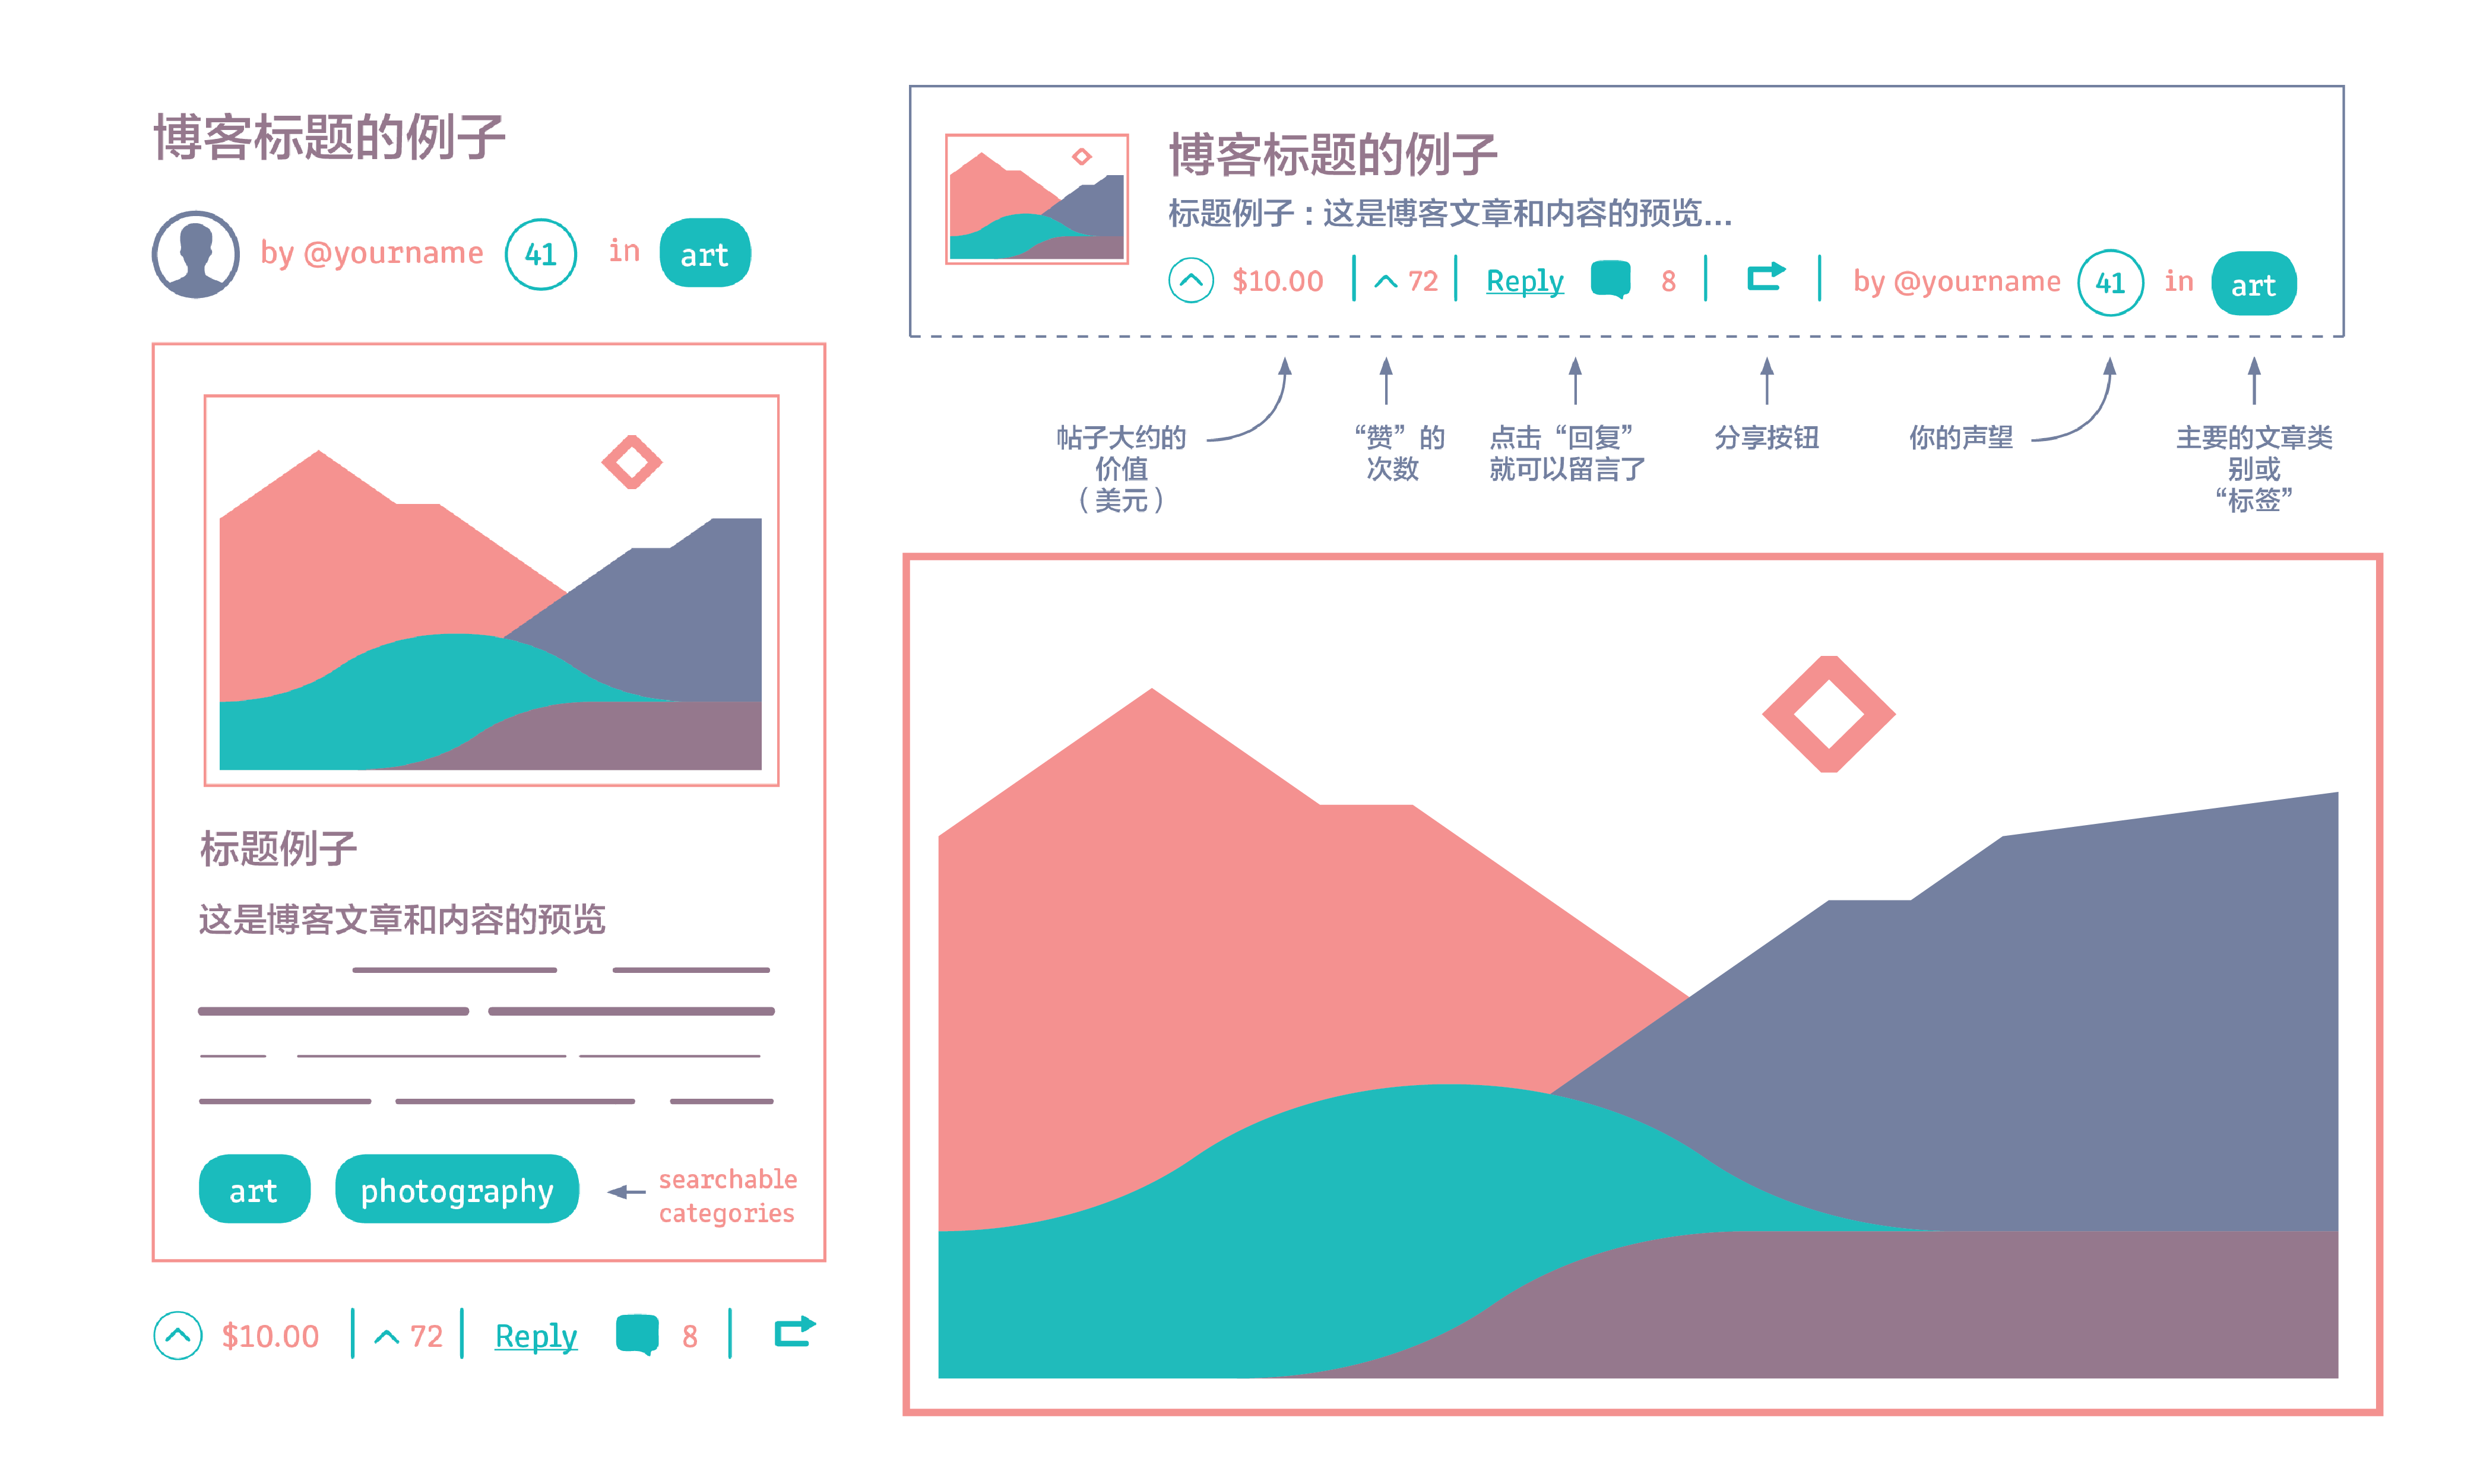
\includegraphics{images/1-1-01.png}

\hypertarget{steemit}{%
\subsection{探索Steemit}\label{steemit}}

终于拿到了Steemit 帐号,可是却不知从何开始浏览Steemit.com?在这个帖子里,我们会教你看一些标签和帖子(见下图),让你可以迅速找到你有兴趣的话题。那么,我们就从Steemit 网上左上方的5个标题开始介绍起:

\begin{itemize}
\item
  首页 (Steemit 按钮) - 在这里你可以看到你所追随博主的帖子。
\item
  流行帖子(Trending) - 在这个标签以下的帖子均为流行帖子,非常鼓励去看看!原因在此。
\item
  最新帖子(New) - 在这个标签以下的帖子均为当下刚出炉的帖子。
\item
  热门帖子(Hot) - 在这个标签以下的帖子均为当下火红并得到一定的点击量的帖子。
\item
  被推广的帖子(Promoted) - 在这个标签以下的帖子都是一些用户自己花费推广的帖子,以便获得更多的阅读量和点击量。
\end{itemize}

如果你想要查找特定标签的最热门和趋势帖子,你可以到Steemit 网页左边那里点击你想要的标签。(见下图)

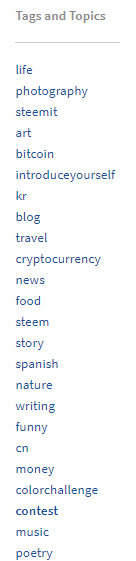
\includegraphics{images/1-1-02.png}

\subsection{预览帖子}

在每一个标签或主题里每个小时都有成千上万的帖子,该如何去筛选出心仪的帖子呢?很简单,你只需要大约看过每一个帖子的预览就能筛选出来。但是每一个预览中都有很多看不懂的意思?别着急,你可以根据以下图片来知道每一个字体或数字的意思。

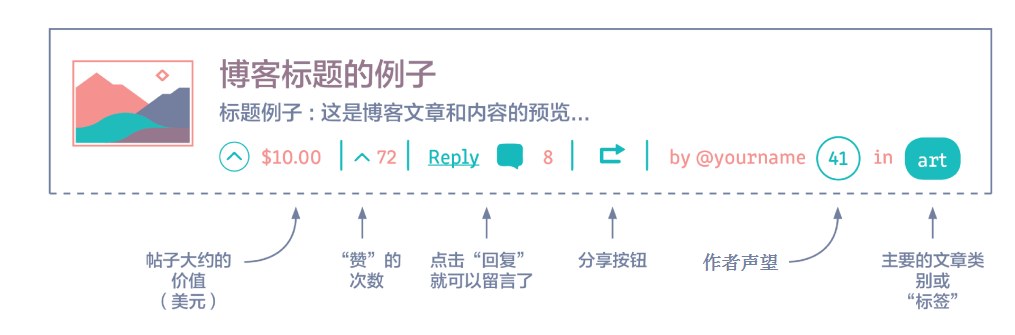
\includegraphics{images/1-1-03.png}

\hypertarget{steemit-}{%
\subsection{Steemit 上如何阅读帖子}\label{steemit-}}

当你点击进入你想看的帖子时,全文窗口就会弹出来。如此一来,你就可以阅读全文。阅读完后,如果你想打赏那位作者,你就点击 ``赞'',而如果你想与作者互动,可以在文章下方点击``reply'' 留言。(见下图)
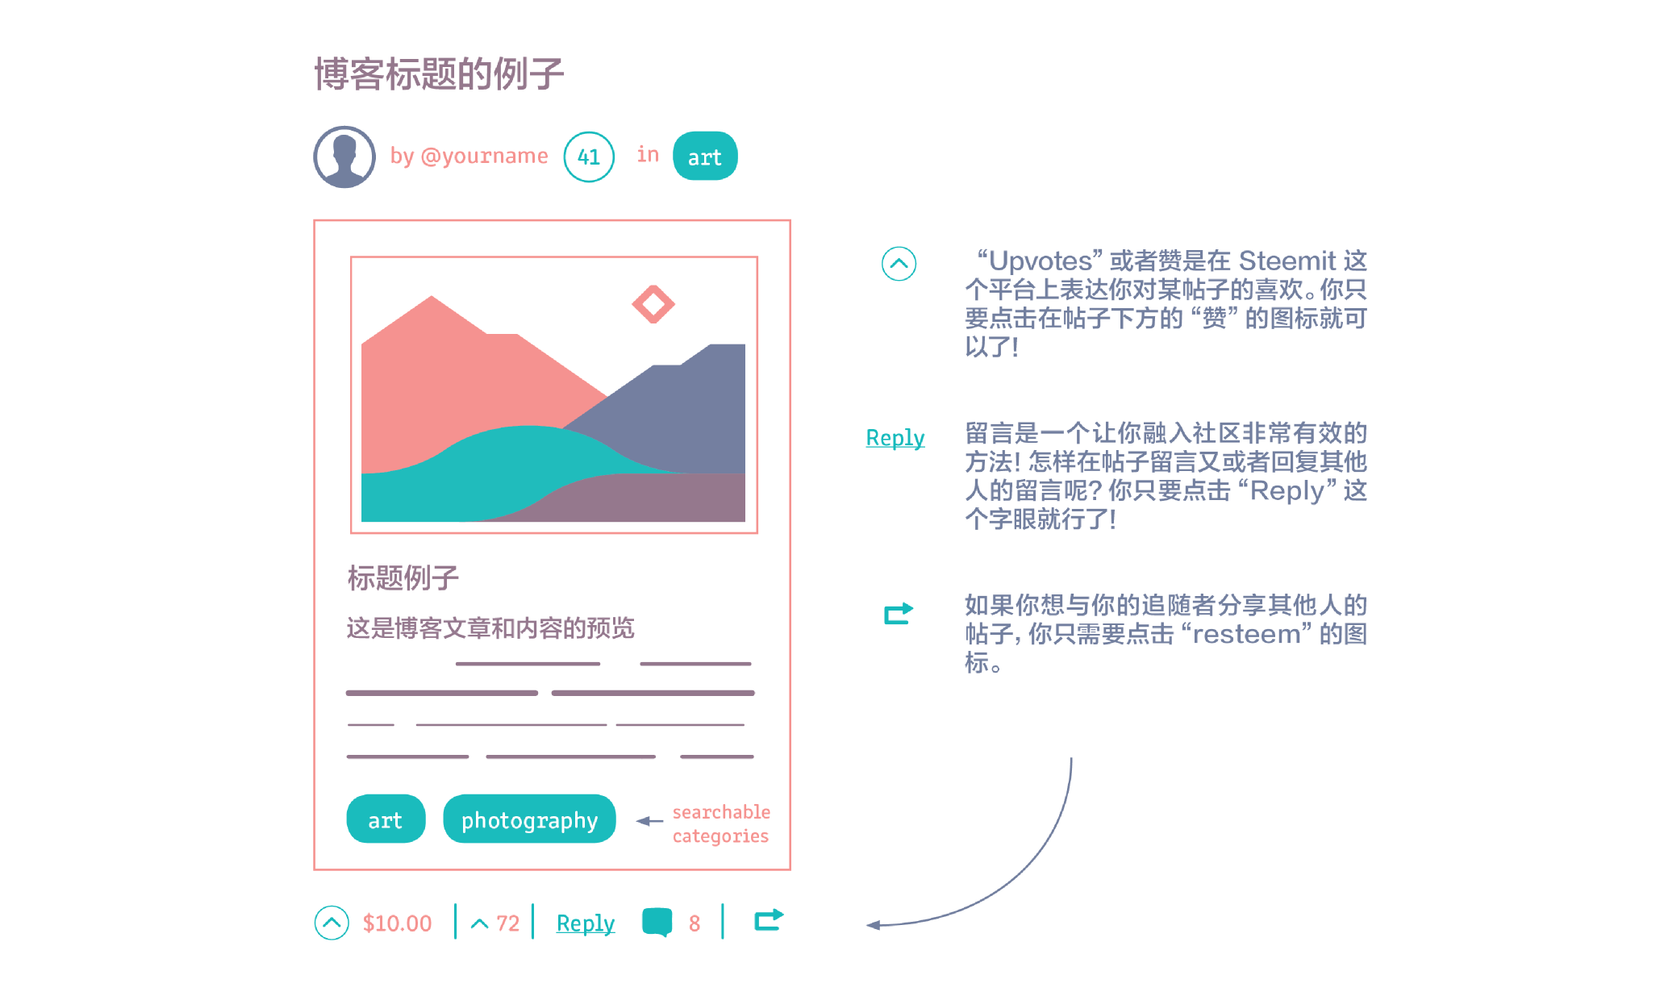
\includegraphics{images/1-1-04.png}

看完后相信你已经对steemit的网站有了初步的了解,接下来,赶紧注册一个账号加入steem的大家庭吧!

\hypertarget{-steem-}{%
\section[注册 steem 账号 ]{\texorpdfstring{注册 steem 账号 \footnote{作者:@maiyude;@hepeng.chn;@ivysrono;@wang-peilin;编辑:@maiyude}}{注册 steem 账号 }}\label{-steem-}}

小雅有点烦躁,因为她在注册Steemit账号时遇到了难题。

这是她见过的注册账号最不友好的社区。她从来没有想过注册一个账号会是那么麻烦的一件事情,她甚至萌生了永远不登陆这个网站的想法。

首先这个网站的浏览速度超级慢,至少在中国访问的速度是超级慢,她感觉回到了拨号上网的时代。其次,注册个账号居然需要翻墙来收取验证码。天啊,她一个小女生哪里懂得翻墙这些高科技的事情啊。

好不容易在朋友的帮助下翻了墙,又专门去注册了一个Gmail的邮箱用来收取验证码,按照步骤一步步的完成注册。忙完这些,她发现刚注册的账号居然还不是马上生效,还要等待官方把你的账号激活,这个过程一般是1-7天左右。

小雅很是抓狂,终于在第三天的早上,她收到了官方发来的邮件,她的账号正式开通了。

虽然历经波折,但是小雅的Steemit之旅正式开始。

\begin{center}\rule{0.5\linewidth}{\linethickness}\end{center}

如同小雅的经历一般,确实注册一个steemit账号对于新人来说有些困难,让我们跟着教程一步步来注册一个新账号吧!

\begin{itemize}
\tightlist
\item
  1.首先登陆steemit.com,点击注册按钮
\end{itemize}

\begin{figure}
\centering
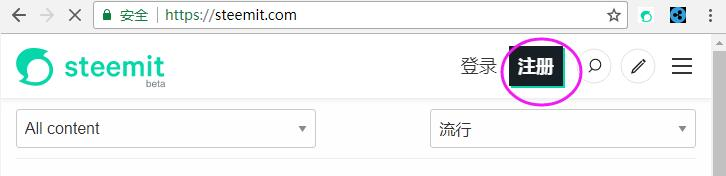
\includegraphics{images/1-2-1.jpg}
\caption{1-2-1.jpg}
\end{figure}

\begin{itemize}
\tightlist
\item
  2.输入你要注册的用户名,只能是英文小写字母
\end{itemize}

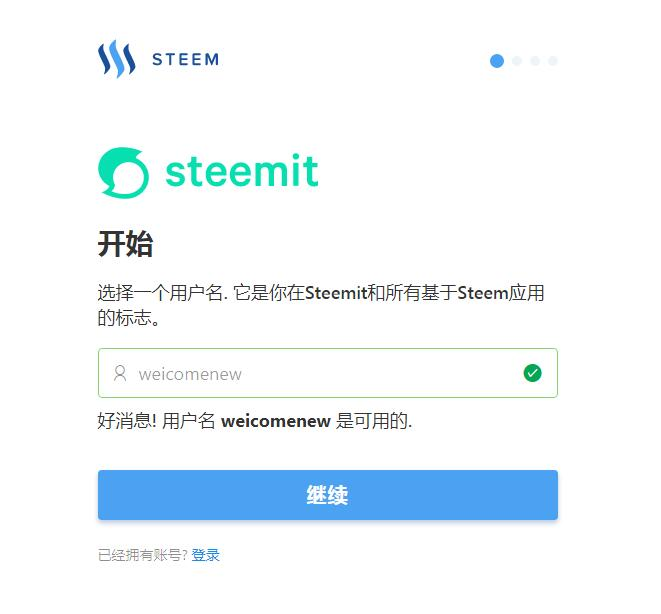
\includegraphics{images/1-2-2.jpg}

\begin{itemize}
\tightlist
\item
  3.输入你的邮箱地址,建议使用gmail邮箱,有部分邮箱可能会收不到验证码。
\end{itemize}

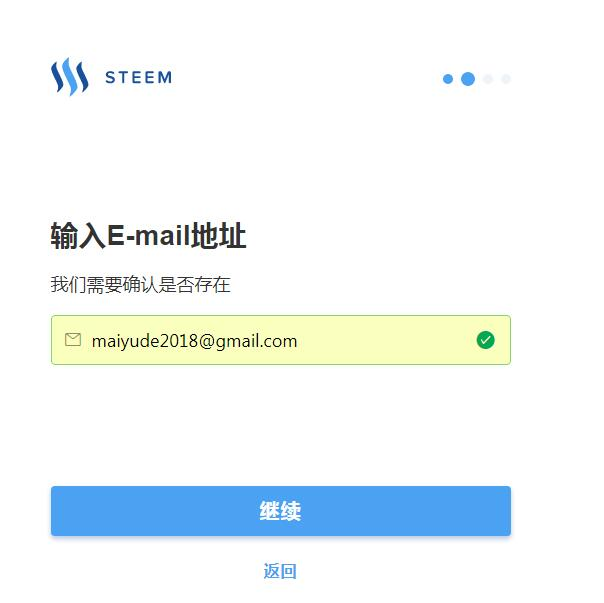
\includegraphics{images/1-2-3.jpg}

\begin{itemize}
\tightlist
\item
  4.官方会发送一份验证邮件到你的邮箱,登陆邮箱查收邮件,点击邮箱内的链接跳转。
\end{itemize}

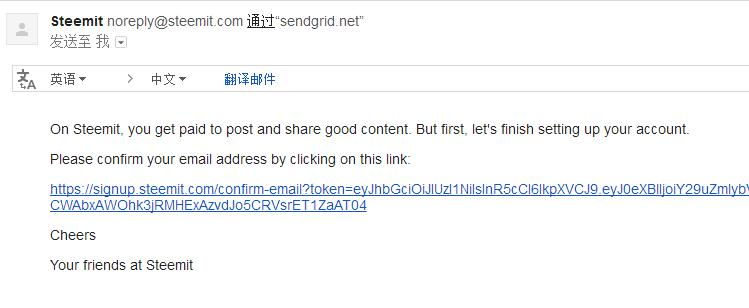
\includegraphics{images/1-2-4.jpg}


\includegraphics{images/1-2-5.jpg}

\begin{itemize}
\tightlist
\item
  5.跳转页面后,输入手机号码接收验证码。这里可能需要打开VPN,有些中国号码无法接收验证码。
\end{itemize}

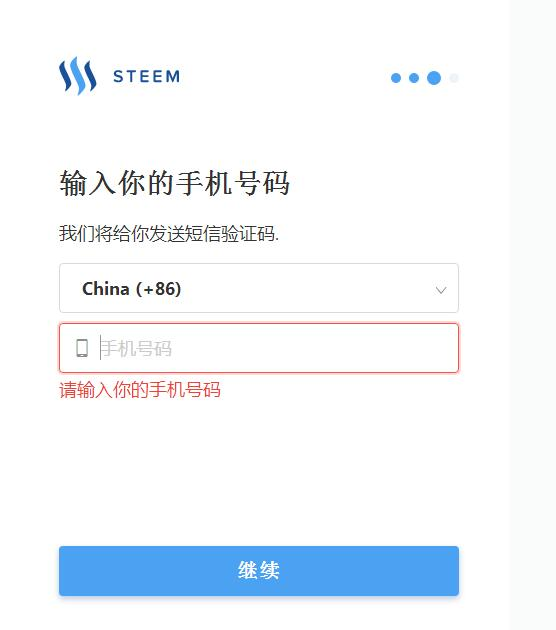
\includegraphics{images/1-2-6.jpg}

\begin{itemize}
\tightlist
\item
  6.填写验证码后,请耐心等待几天,官方需要审核你的信息。审核完毕后,会再次向你邮箱发送邮件。
\end{itemize}

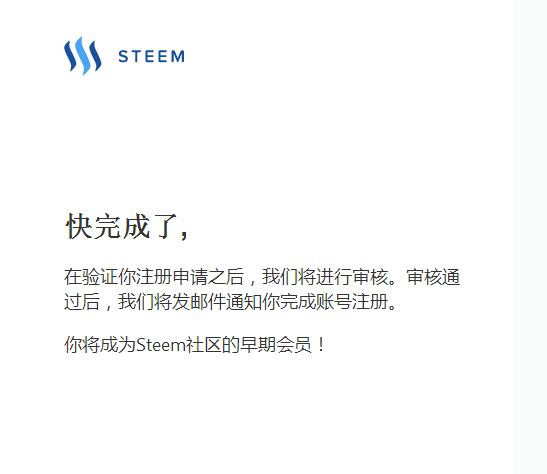
\includegraphics{images/1-2-7.jpg}

\begin{itemize}
\tightlist
\item
  7.打开邮箱,点击邮件内的链接跳转,记录好密码,请妥善保管你的密码,这个密码非常的重要。提示注册完成。
\end{itemize}

\includegraphics{images/1-2-8.png}

由于官网注册需要等待一段时间,有些朋友可能有点不耐烦,那么有没快速注册的方法呢?当然是有的,下面介绍一些快速注册的方法(需要付费)。

\begin{itemize}
\tightlist
\item
  \href{https://cnsteem.io/}{付费注册}:
\end{itemize}

\url{https://cnsteem.io/}

\begin{itemize}
\tightlist
\item
  依次输入\texttt{用户名},\texttt{邮箱地址}。
\item
  点击去支付宝付款,支付\$2费用(约¥12)。
\item
  支付完成后,邮箱将收到注册链接,获取\texttt{密钥}。
\item
  注册完成。
\end{itemize}

\textbf{ps:}密钥需妥善保管,丢失无法找回,建议多备份以免损失。

\begin{center}\rule{0.5\linewidth}{\linethickness}\end{center}

两种方法各有优缺点,可酌情选择。

\begin{longtable}[]{@{}ll@{}}
\toprule
官网注册 & 付费注册\tabularnewline
\midrule
\endhead
需要翻墙 & 不需要翻墙\tabularnewline
5-7天审核期 & 立即完成\tabularnewline
免费 & 付费\tabularnewline
初始有效15sp & 初始有效2.2sp\tabularnewline
\bottomrule
\end{longtable}

另外如果你已经拥有一个账号,也可以通过你的账号来创建新账号,需要确保你账号内有一定数量的steem。

\begin{itemize}
\tightlist
\item
  步骤
\end{itemize}

\begin{enumerate}
\def\labelenumi{\arabic{enumi}.}
\item
  已有一账号。
\item
  登录 \url{https://steemconnect.com/}
\item
  访问 \url{https://steemconnect.com/apps/create} 阅读提示:\texttt{The\ current\ fee\ for\ create\ a\ new\ account\ is\ X.000\ STEEM.}
  当前数值为 3:
  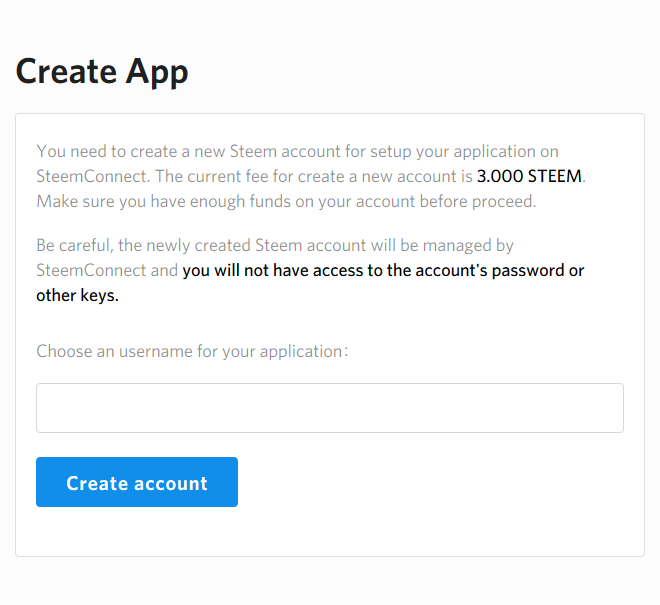
\includegraphics{images/1-2-9.png}
\item
  在原账号中准备不少于上述提示数量的 STEEM 。
\item
  访问 \url{https://steemconnect.com/accounts/create} 或\url{https://v2.steemconnect.com/accounts/create}
\item
  在 \texttt{Username} 中输入新账号的用户名------切记,没有大写字母!
\item
  备份好 \texttt{Password} ------机会只有一次!
\item
  将 \texttt{Steem} 中 \texttt{0.000\ STEEM} 改为 \texttt{Y\ STEEM}。啰嗦一句,Y\textgreater{}=X.
\item
  点击 \texttt{Continue} 并按照提示输入密钥即可。
  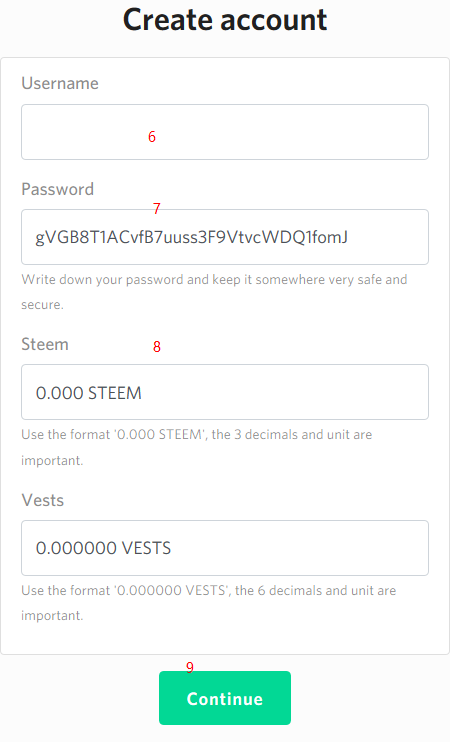
\includegraphics{images/1-2-10.png}
\item
  特别说明:新账号会自动拥有 \texttt{Y} 个 SP;\texttt{Vests} 可以保留0,否则会换算成 SP 代理给新账号,经过\href{https://steemit.com/cn/@oflyhigh/o-sp}{一段时间}后可以收回。
\end{enumerate}

\section[登录 ]{\texorpdfstring{登录 \footnote{作者:@dapeng,原文链接:\url{https://steemit.com/steemit/@dapeng/the-very-first-thing-to-do-for-new-steemians-or-steem}}}{登录 }}

小雅好不容易注册好了steemit账号,终于可以开始她的steemit之旅了。

作为 Steem 新手,必须做的最要紧的事情是什么?是兴奋地发第一帖宣告自己的降生吗?是看看收益最高的帖子来学习如何在 steem 赚钱吗?还是上传自己帅帅的头像呢?

小雅听说,第一件事,至关重要的任务,是立刻抓起你的相机,对着显示器上的 steem 密码拍个照片,打印到纸上,删掉数码照片,然后把这张纸塞到一只鞋子里,藏在床底下。

\begin{center}\rule{0.5\linewidth}{\linethickness}\end{center}

曾经有一次,有个声望达到 67 的账号被坏蛋机器人 \citet{cheetoh} 用钓鱼手段骗过了眼睛。这个盗贼看上去很像著名的机器人 \citet{cheetah}。价值数万人民币的 SP+SBD 和无法估量的其他损失,就这么进了别人钱包,让人痛心。找回密码和账号很困难,几乎是不可能的。

steem 新手注册成功后,会得到一个很长的字符串。官方称其为``万能钥匙'' (master/owner key)。这很容易让新手误以为是个登录密码。别的网站不都是如此吗?忘就忘了,不都是能用邮箱或手机恢复吗?于是,他们首次登录,愉快地发布第一帖,读了一些别人的文章,然后关掉了网页,把一切都抛诸脑后。几天之后,他们突然想起了 steem,想登录看看自己是不是赚了点钱。可是那么长的密码,谁记得住呢?恢复一下吧\ldots{}\ldots{}居然不能恢复??!!

新手并未被充分告知密码的重要性。在中文微信群里,曾有个用户不小心把密码复制粘贴出来,每个人都看见了。还有个用户,把他的钱包-权限页的四个密码截了屏,一起发给我,问我这些是什么意思。没人钓鱼欺骗他们,他们只是不知道他们自己在做什么。

现实生活里,如果丢了身份证,可以去身份证中心------派出所或警察局补办。如果丢了信用卡,可以去信用卡中心------拨打服务热线挂失。Steem 的世界里,如果丢了密码,对不起,没有哪个中心可以去,因为 Steem 用的是区块链,去中心化!

实际上, steem 用户的主密码不只是个密码,而是个多合一的混合体,相当于:

\textbf{Steem 主密码 = 登陆密码 + 身份证 + 银行卡 + 手机 + 签名}

只要有了你的主密码,任何人都可以在 steem 上登录你的账号,转账,发帖,给别人留言,钓鱼欺骗你的朋友。这玩意儿到底应该叫什么?''万能钥匙/主密码`` (Master/owner key) 这个称呼远远不够。我觉得应该管它叫''Steem 账号的命根子``。一旦丢失,就是死路一条。

永远不要使用你的主密码!

钱包(Wallet)-权限(Permissions)页面有四个密码。

\begin{itemize}
\item
  登录的时候,用发帖密码(posting key),足够平时使用。
\item
  只有在跟钱打交道时,才使用活跃密码(Active key)。
\item
  那么主密码是干什么用的?只有重置账号时才用。你可以当作是手机上的``恢复出厂设置''。这个功能应该大部分人都很少用过,是不是?
\end{itemize}

所以,最好把主密码打印出来,塞到鞋子里,藏到床底下。

就像科幻小说《三体III》里所讲,如何保存资料最安全? 刻在石头上!

\section[密码的保管 ]{\texorpdfstring{密码的保管 \footnote{作者:@vickylin 编辑:@vickylin}}{密码的保管 }}

登陆过程比较简单,这里不做冗述。值得一提的是,注册时提供的是master password,首次登陆后,把posting key和active key保存下来后,再也不要用该密码登陆。在日常使用中,我们可以用posting key来发帖、点赞、回复,用active key交易、转账。

关于密码的保存,我个人会使用种方法:\textbf{密码管理器、加密盘、硬盘和纸质}。

\hypertarget{u}{%
\subsection{硬盘/U盘}\label{u}}

如果你选择这个办法,最好找个硬盘/U盘专门做保存密码所用,其他文件一概不放入,并且平时做好杀毒工作。

\subsection{纸质}

有些人可能会嘲笑这种最原始的做法,心想着什么都往电子化数据化的时代靠,谁还有人拿纸笔记录下这一切。在丢失密码的那几天,我曾去请教过一位大神,他是如何保存重要密码的。他笑着说:
\textgreater{} 我用小本子记下来呀。

因此,无论你通过数据化的方式做了多少备份,重要密码纸质的一定要有一个,无论是手抄还是打印,然后放在一个安全且你绝对能想得起来的地方妥善保管。

\subsection{密码管理器}

现在市面上比较主流的是1Password、keepass和lastpass等。当然,如果你要让我把密码记录在word、excel或者note里面,那我们可能不在谈论一件事情。lastpass我没有用过,主要谈谈另外两种。

1\textbf{Password}

这是我接触的第一个密码管理器,界面非常简约好看,操作上也无任何问题。如果产生疑问,可以发邮件给他们的客服,客服人员非常认真负责,会尽可能的去帮助你。当然,因为其公司在加拿大,故而会有时差,一般来说你今天发的邮件第二天可以收到回复。个人使用过程中没觉得有什么缺点,一定要讲的话,就是贵。

1Password是采用一次买断和订阅式的。如果你打算长期一直用下去的,推荐买断,听朋友说大概是五百多。订阅的话是一个月27rmb(在网页版登录后有看到2.99\$/mon,但需要绑定信用卡,并且需要输入信用卡CSV码,个人觉得不是很安全放弃了)。另外,windows和mac是要分开购买的,也就是说一个账户无法跨平台使用。

使用1Password的朋友们务必记得以下三点:

\begin{enumerate}
\def\labelenumi{\arabic{enumi}.}
\item
  注册完以后,记得把emergencykit保存好,里面涵盖了用户名及secret key,你也可以打印出来,手写上master key,然后找地方放好;
\item
  登录主界面(可选择指纹解锁的那个界面)的密码,并不一定是你的master key,所以这两个密码如果不同,请务必记清楚;
\item
  可以的话,请在两个设备登录。如果你不小心在一个设备登出(log out)但是不记得密码,另外一台设备也许可以挽救这一切。
\end{enumerate}

\textbf{Keepass}

朋友说,KeePass的缺点很明显,那就是没有浏览器插件,不论是注册还是登陆都要在软件内复制过去。个人觉得这个缺点其实还好,毕竟大部分情况下我们在使用个人电脑的时候,都会选择让浏览器记住密码。一定要讲缺点的话,可能就是界面不如1P来的美观。优点也是显而易见的,它是一个完全免费的开源软件。

下载

\href{https://keepass.info}{官网}我下载的是keepassX。下载好以后直接拖进application即可,因为我用的是macos系统,下面截图演示就是Mac情况下的界面,windows也差不多。

安装及使用

打开软件后点击左上角数据库---新建---输入主密码,确认以后进入这个界面

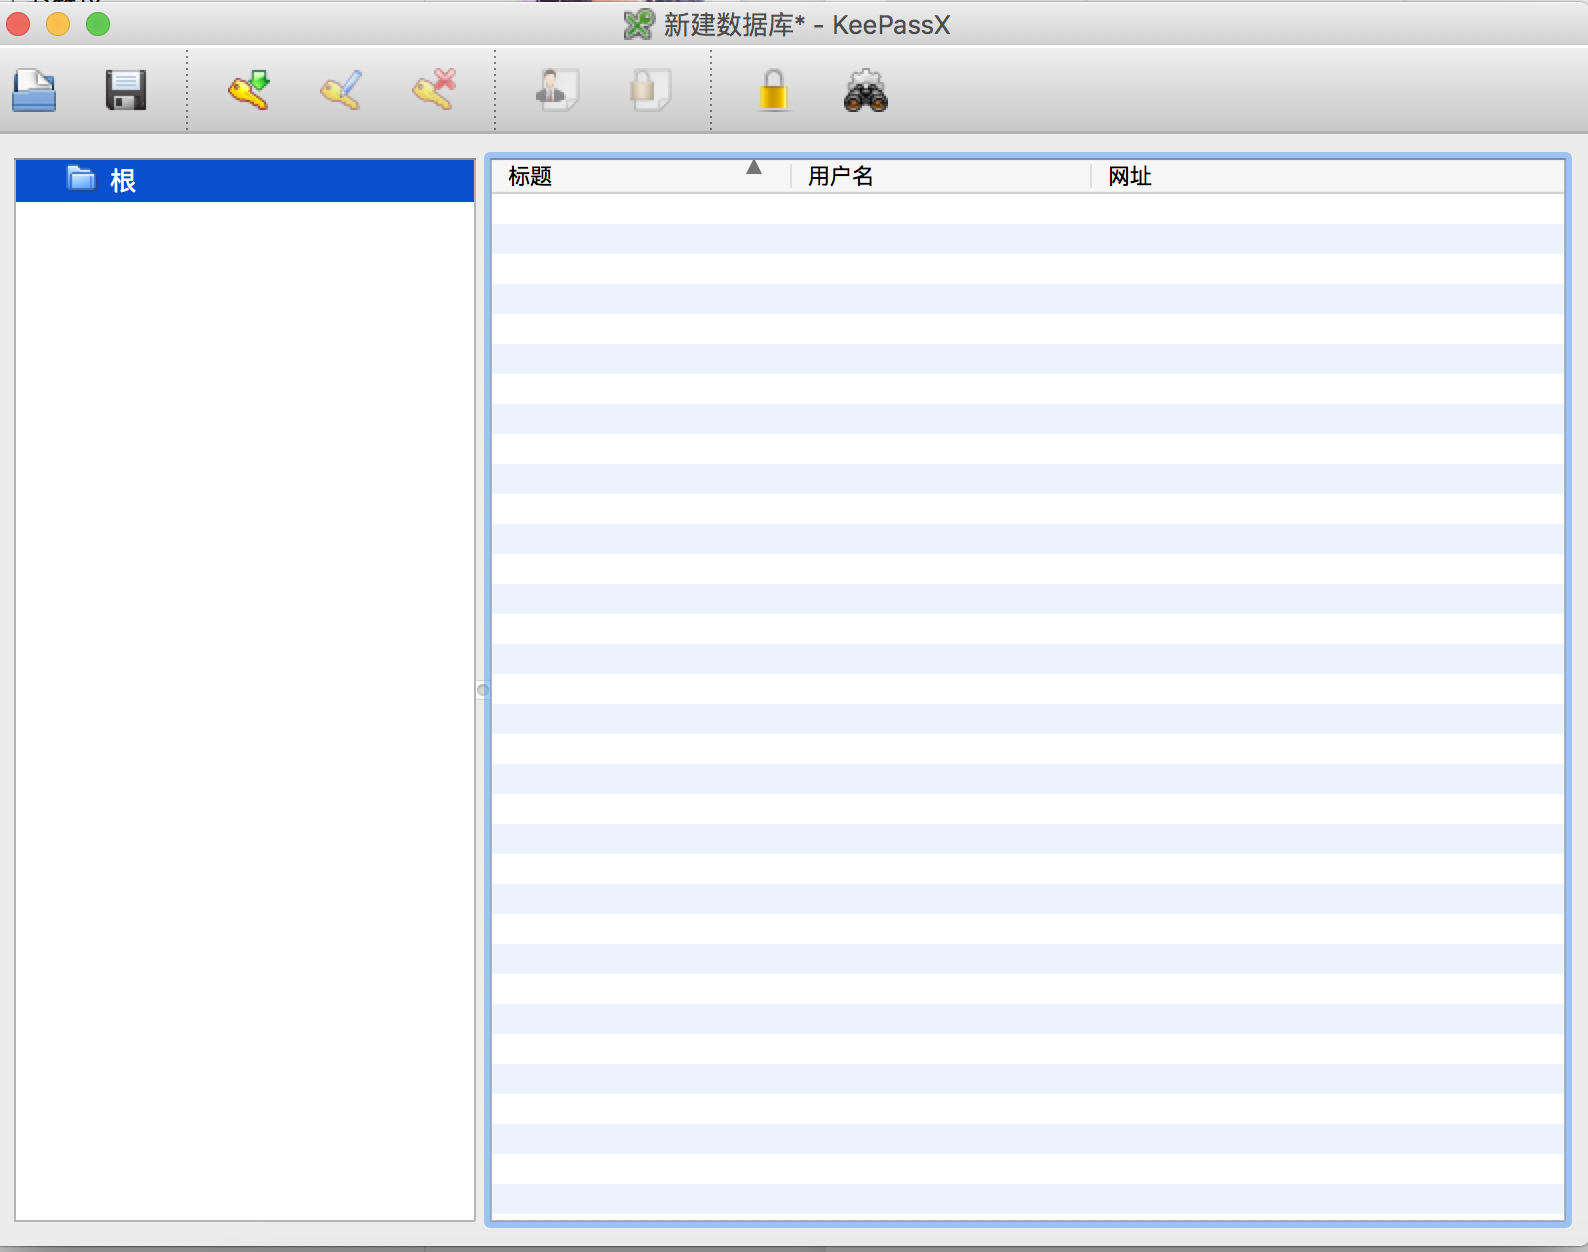
\includegraphics{images/01-keepass01.png}

点击添加按钮,如下图,就可以开始填写/生成密码了,OK以后按保存即可,会形成一个文件(有点类似word保存以后形成的文件)。

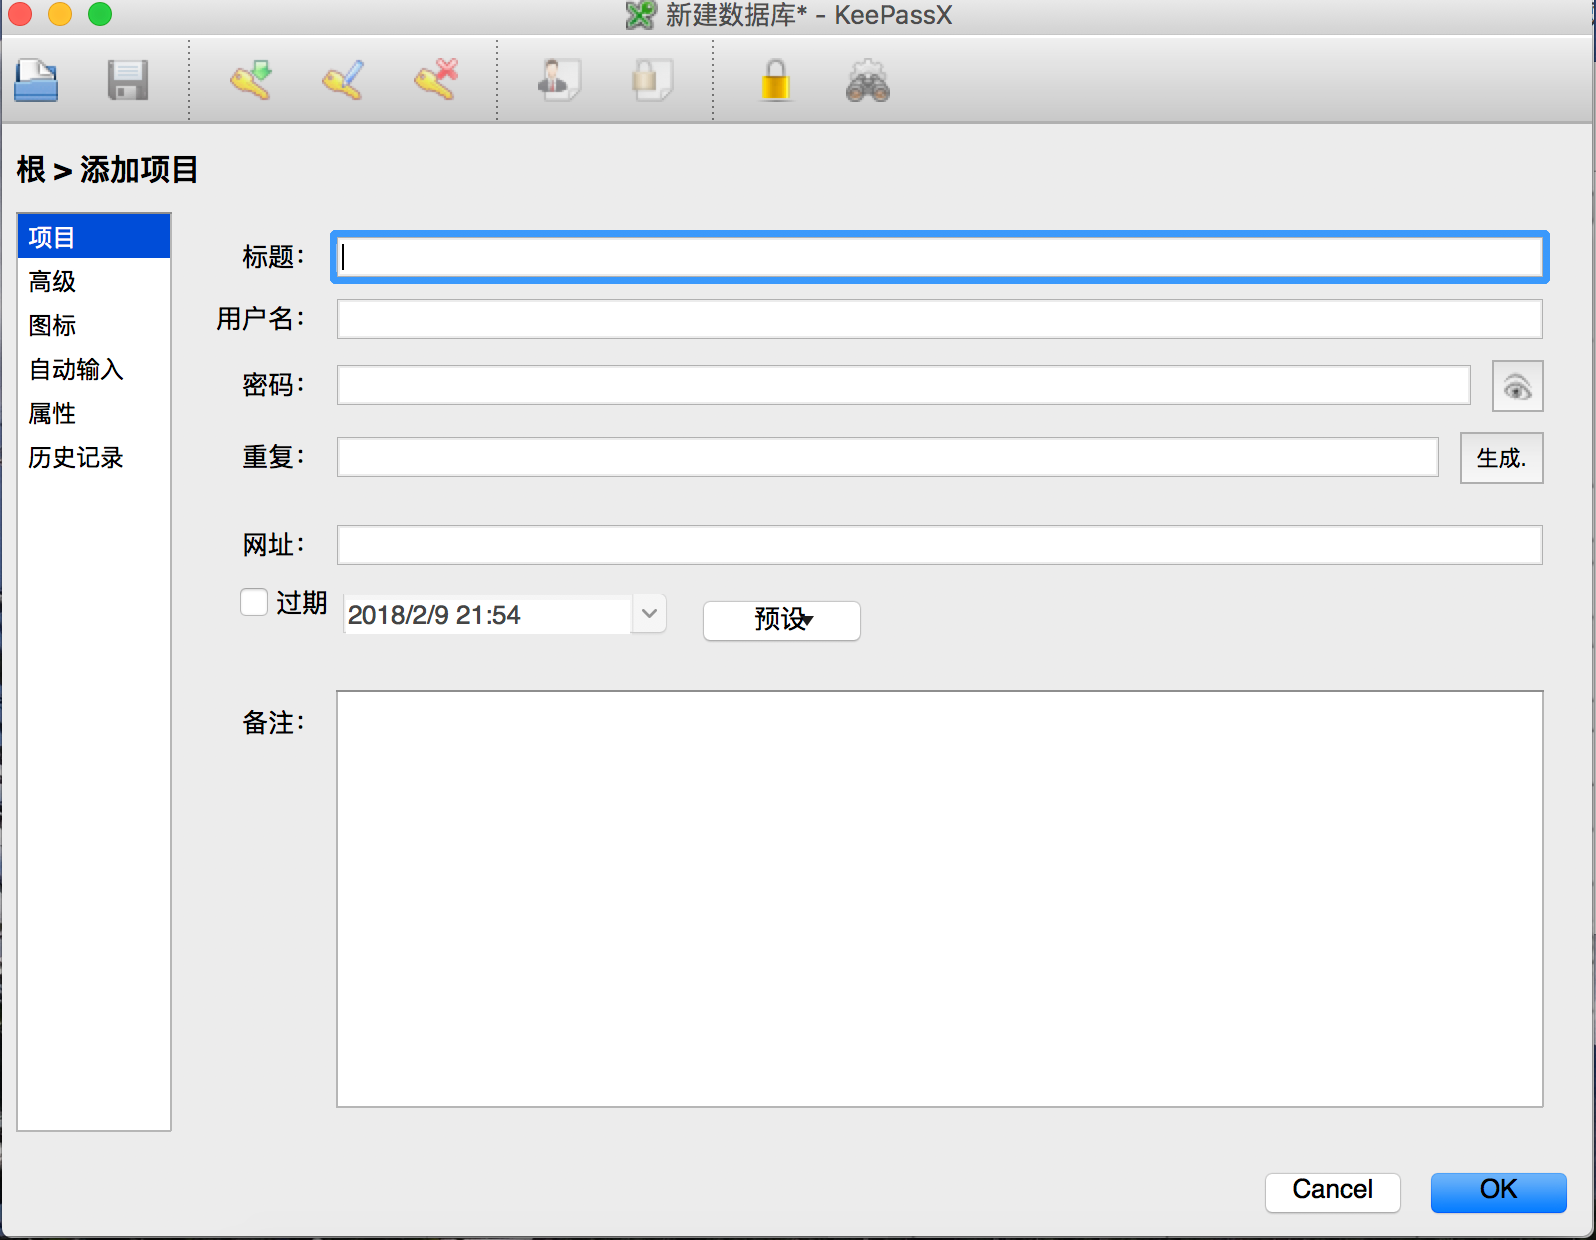
\includegraphics{images/01-keepass02.png}

以后无论点击这个文件,还是keepass的图标,都可以打开这个界面。建议大家输入密码的时候可以把可视选项打开,以免输入的时候错误。

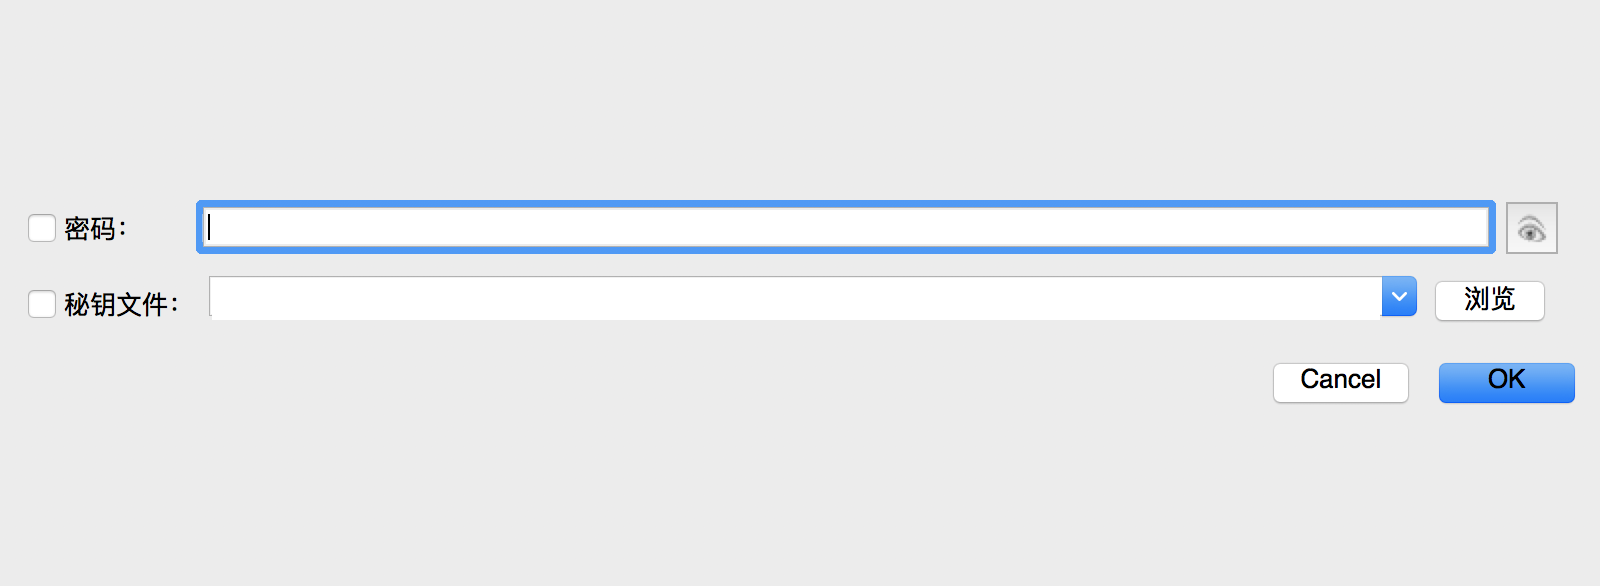
\includegraphics{images/01-keepass03.png}

移动端

我试了keepass touch和mini keepass,个人觉得没什么太大的差别,就用了前者。目前还没有弄好dropbox自动同步,解决方法是将keepass.kdbx的文件丢到dropbox,打开dropbox然后选择用keepass打开即可。在数据库没有更新的情况下,基本打开过一次,这个数据库以后就可以直接在keepass touch里面打开了。

\subsection{加密盘}

在前阵子经历密码丢失后,这段时间我都在备份自己的各种数据。目前我采用了四种方法:keepass+1Password+dropbox+纸质版。强迫症大爆发的情况下,又研究了如何在本地放一个加密盘的方法。

对于用户来说,考虑加密软件主要会从安全性、是否免费及是否多平台等几个方面考虑,那这些方面Veracrypt基本都具备了。VeraCrypt 的前身是 TrueCrypt(2010年有报道称,FBI也无法破解TrueCrypt加密的文件),由于后者被 Google 爆出严重的安全漏洞,这才诞生了 VeraCrypt。同时也说明了,VeraCrypt 具有更高级别的安全性。

下面我们就来看看如何使用\textbf{VeraCrypt}:

安装与设置

1、首先在\href{https://www.veracrypt.fr/en/Downloads.html}{官网}下载;

2、下载完后双击图标,进行安装;


\includegraphics{images/01-VeraCrypt01.png}

3、如果出现以下界面,按照提示,前往\href{https://osxfuse.github.io}{Fuse}下载安装驱动。然后就可以安装VeraCrypt,一路下一步即可;

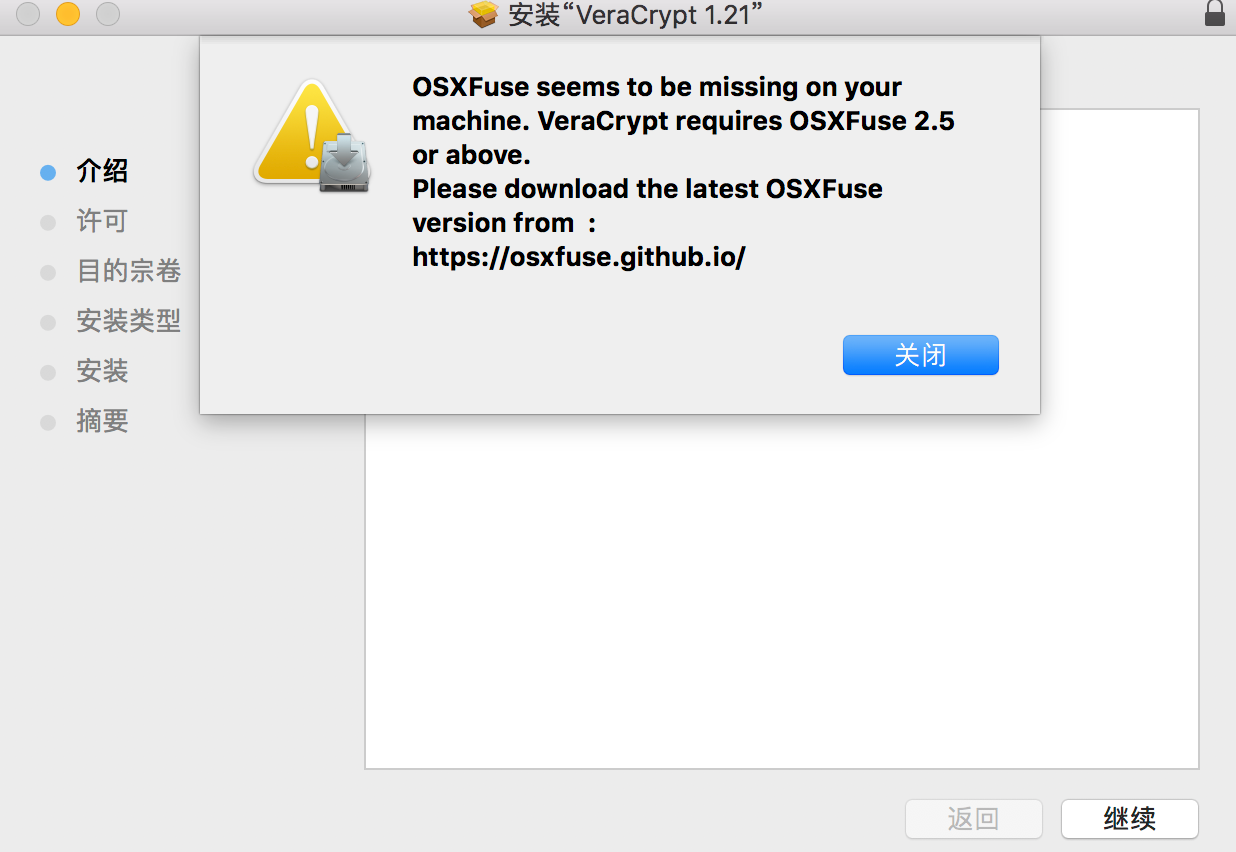
\includegraphics{images/01-VeraCrypt02.png}

加密数据步骤

1、接下来创建加密卷,一般都是默认的选项,下一步即可;

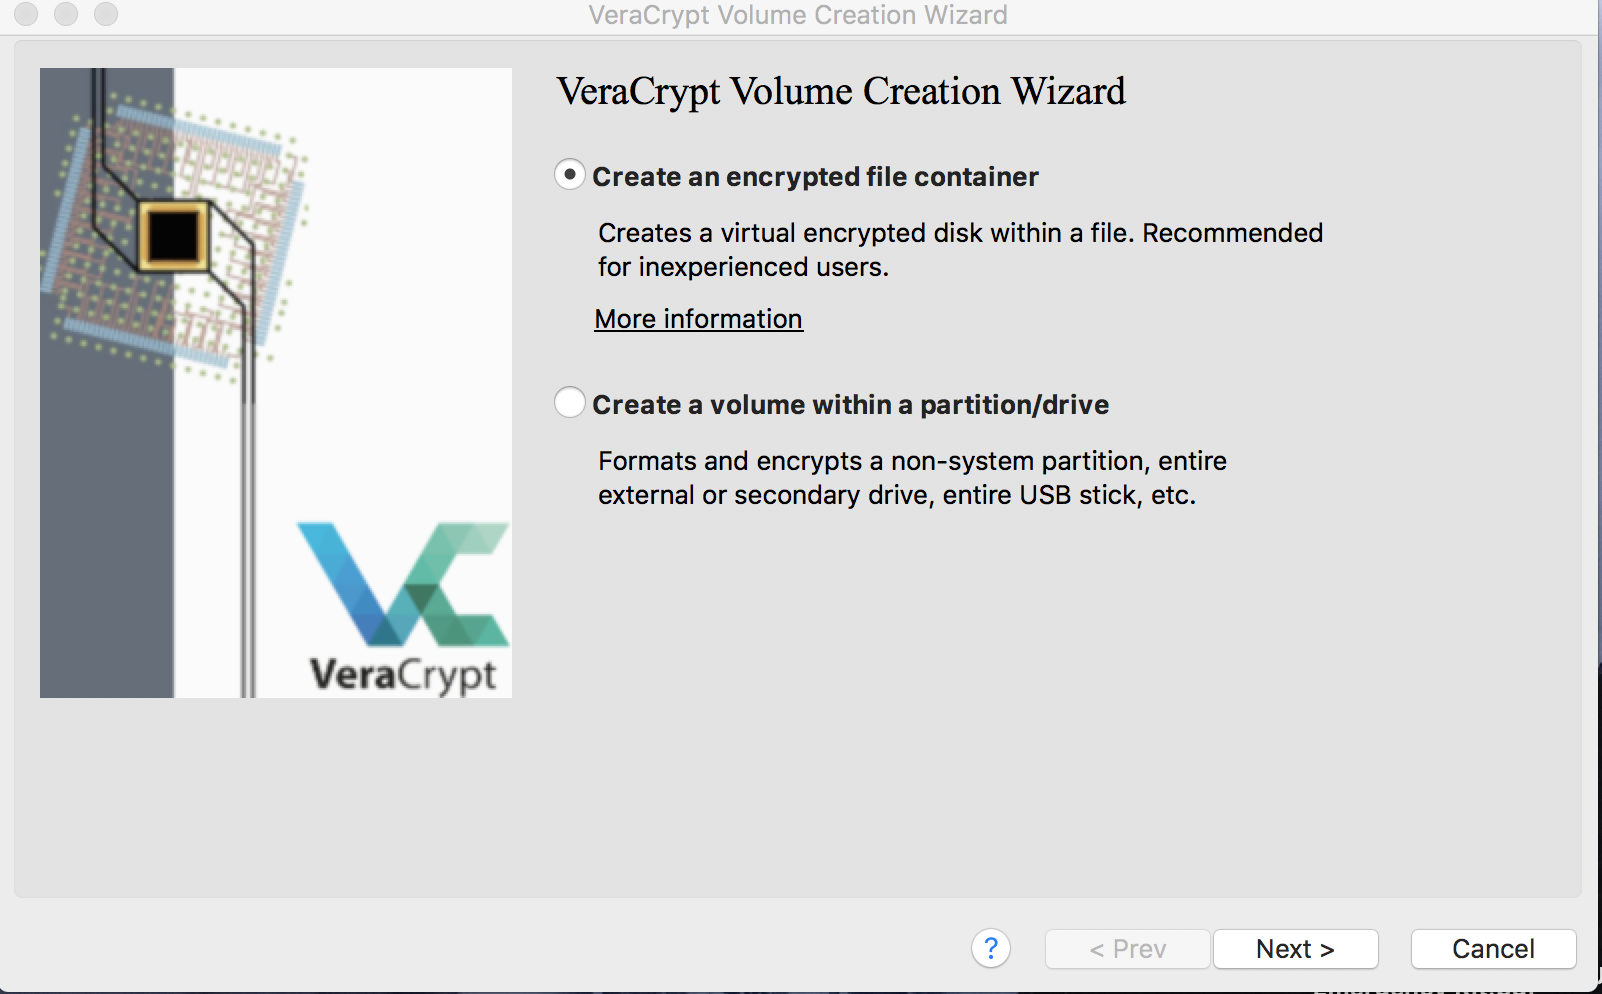
\includegraphics{images/01-VeraCrypt03.png}

2、根据要加密的文件设置加密盘的大小,如果只是保存密码的话,一般1M就够了;

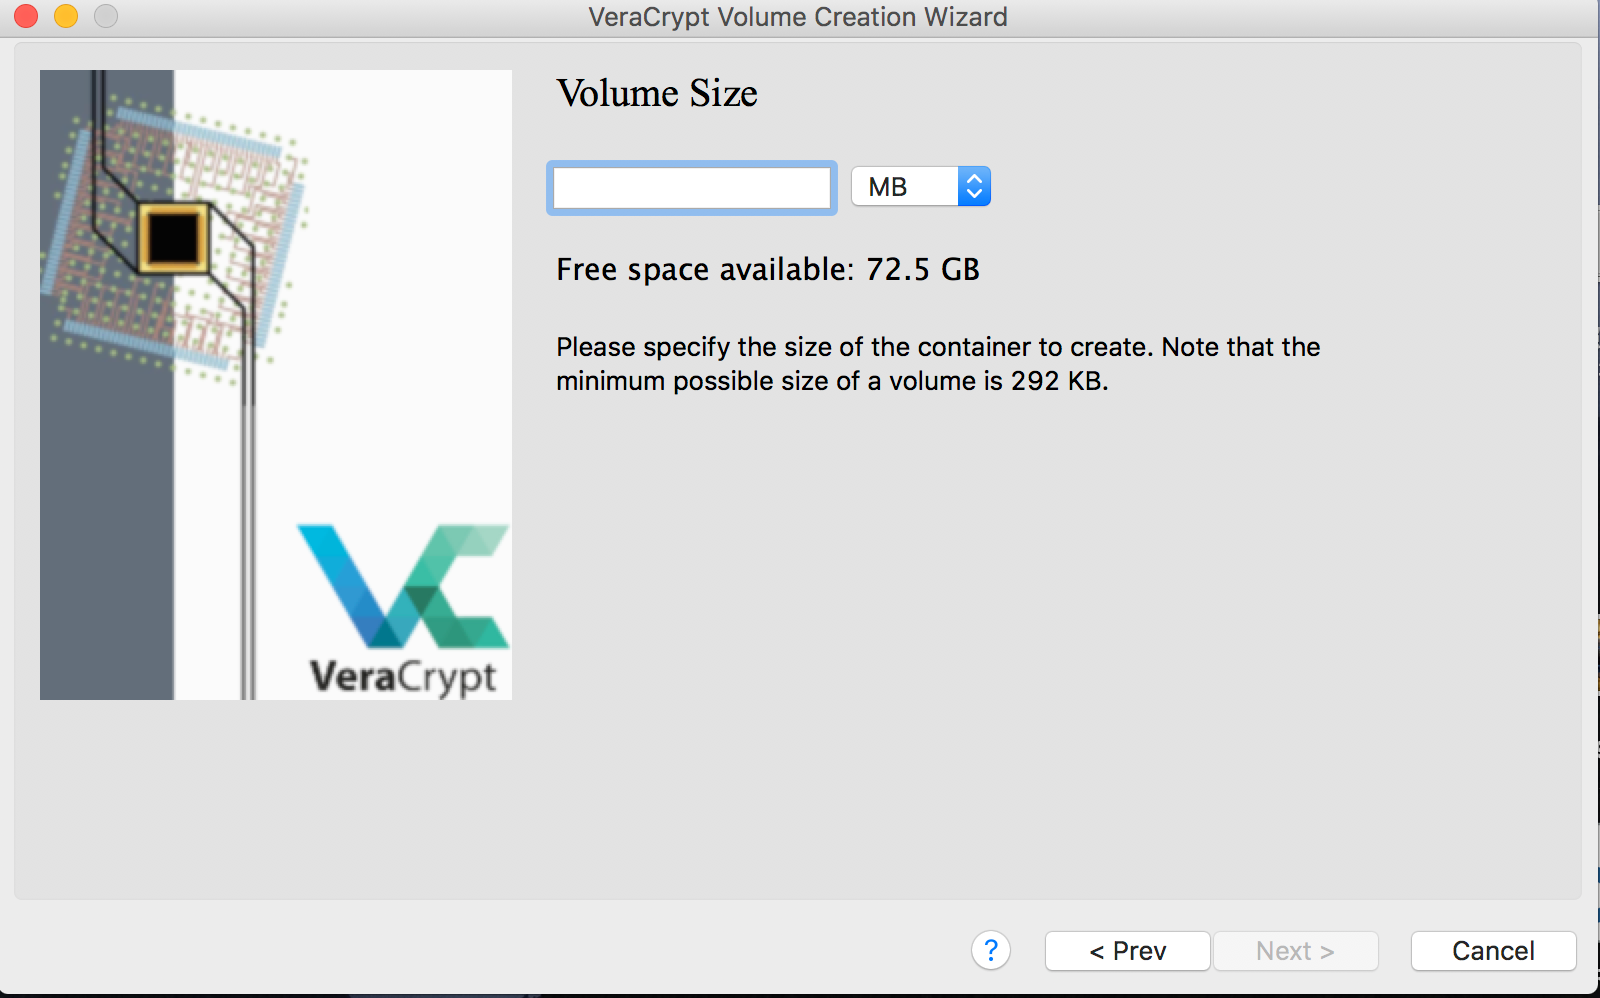
\includegraphics{images/01-VeraCrypt04.png}

3、然后设置密码(我没有使用秘钥文件,听说比较麻烦)。格式化完成后,确定并退出。这个时候你会看到已经加密好的文件,它没有后缀,也无法打开。

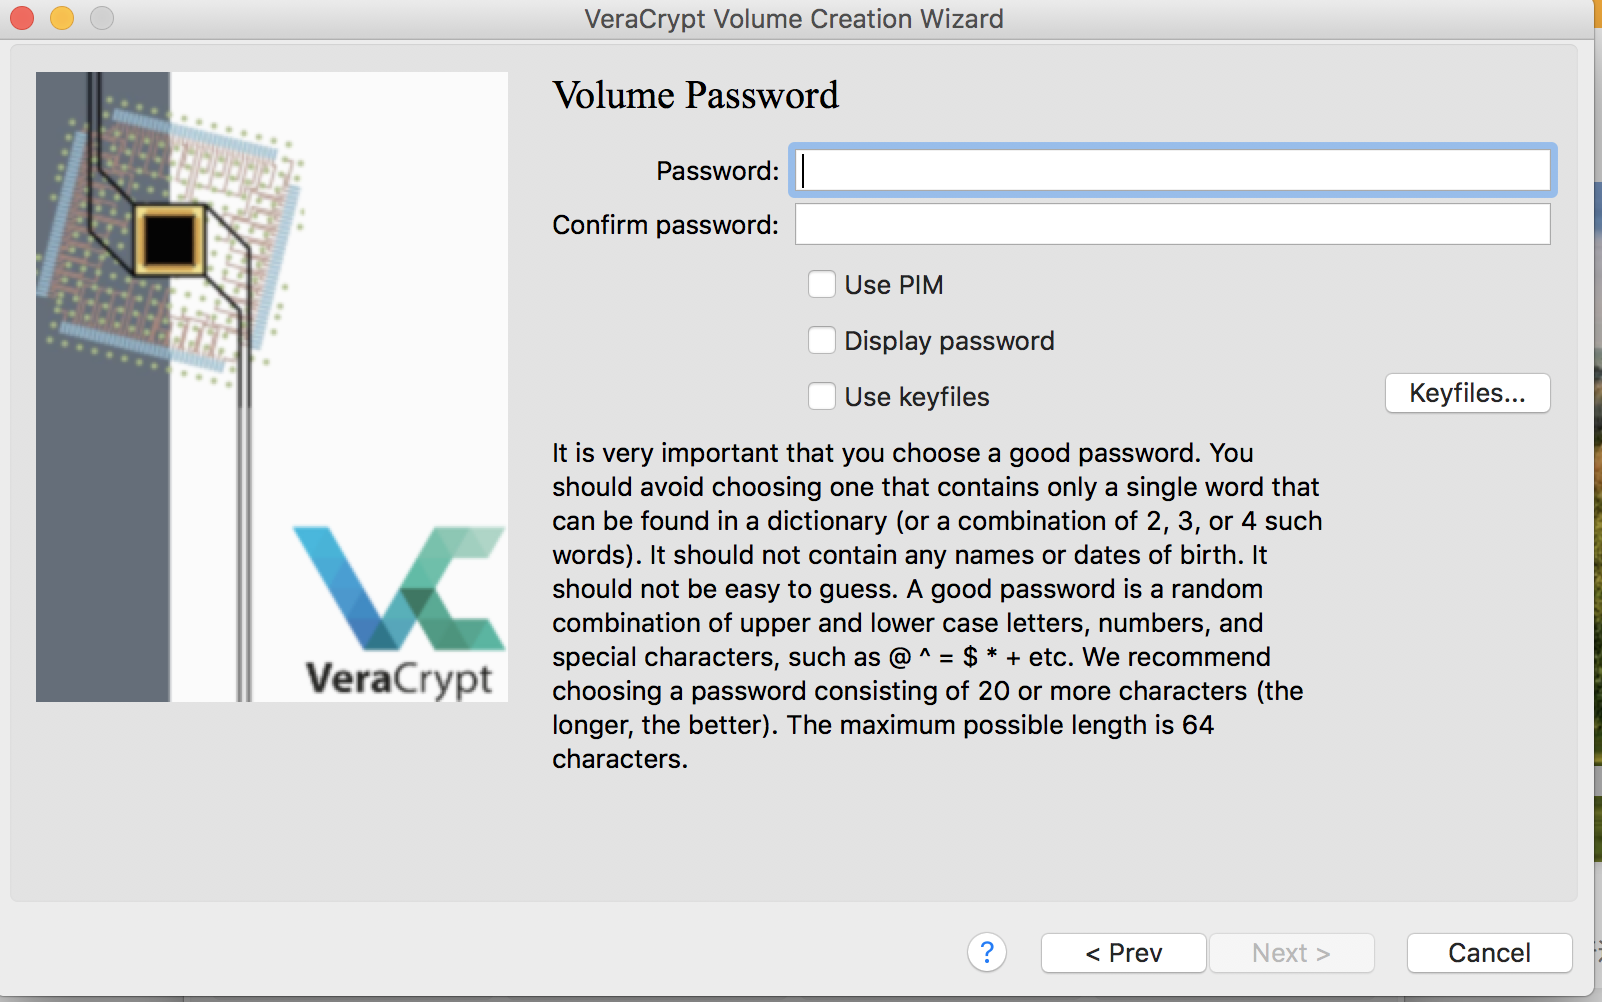
\includegraphics{images/01-VeraCrypt05.png}

解密数据

1、选择加密盘的所在位置,点击加载。如此就可以打开加密盘,可以任意读取盘内的内容,也可以把想要加密的东西丢进去;

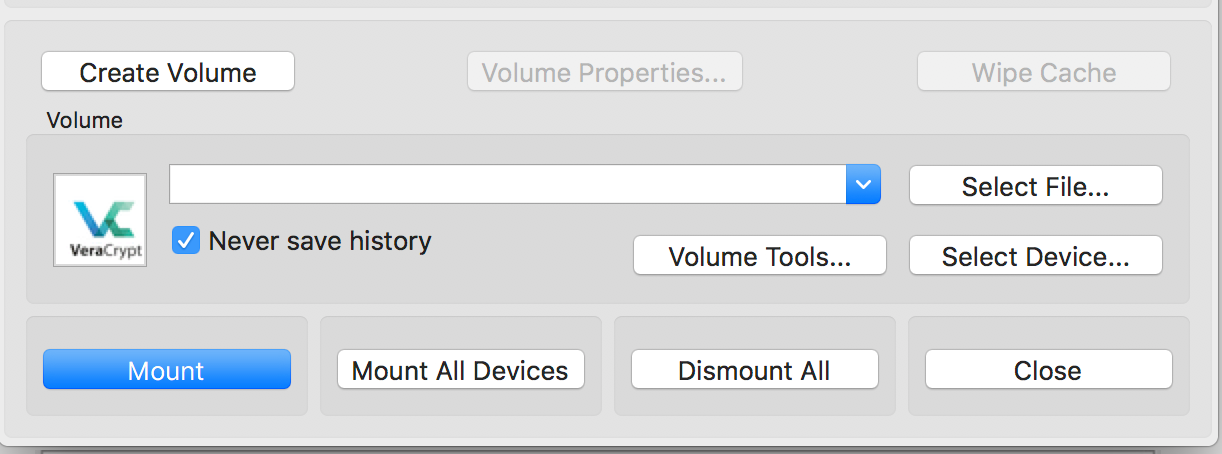
\includegraphics{images/01-VeraCrypt06.png}

2、看完以后,务必点击卸载。这时候,此盘就重新加密,除了有密码的情况下都无法打开;

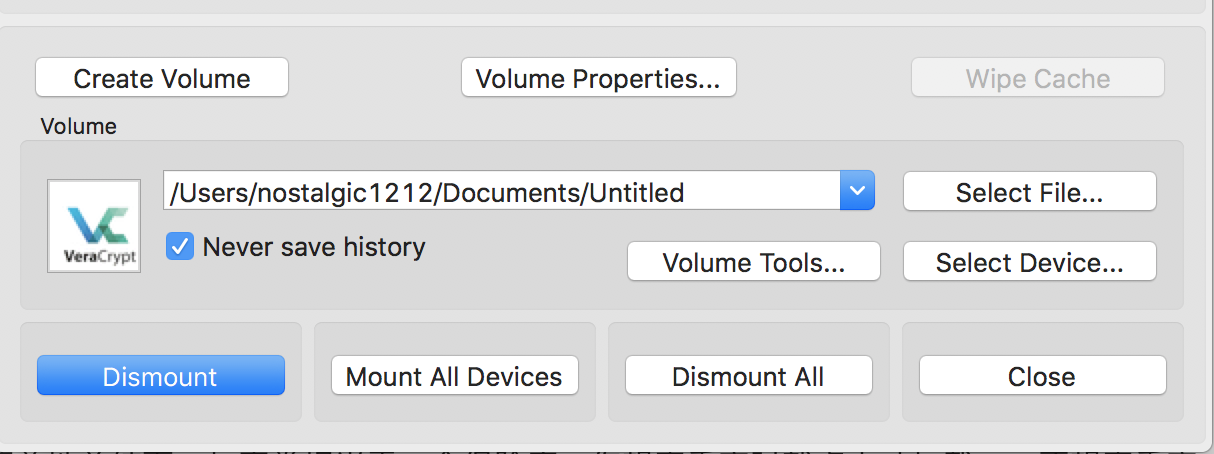
\includegraphics{images/01-VeraCrypt07.png}

注意

1、加密盘的文件名不要随意更改,我测试过,改过文件名的,软件可能会无法打开,出现密码错误的字样;

2、放入文件的时候注意文件大小,不能超过设定的磁盘的大小。

\begin{center}\rule{0.5\linewidth}{\linethickness}\end{center}

于是,小雅首先按照网站的说明把那长达二十多位的密码抄了在一个小本子上。网站上一再提示这个密码非常的重要,遗失了几乎不可找回,这让小雅有点心惊。因为小雅忘记的账号密码不计其数,忘记的概率远远大于被盗的概率,很久不登陆的账号她都是通过重设密码才找回的,这个网站的密码不可找回让她有点担忧。小心驶得万年船,她把密码抄了下来,又在加密的云盘上保存了一份,她想这样应该不会忘记了吧。

忙完密码的事情,她寻思着如何装修一下自己的个人主页。

\section[设置个人基本信息 ]{\texorpdfstring{设置个人基本信息 \footnote{作者:@maiyude}}{设置个人基本信息 }}

小雅点进了自己账号的设置页。

Steemit的各种设置和博客有点类似,虽然小雅的博客随着微博微信的兴起荒废多年了,但是小雅以前可是一个博客迷呢。

首先要设置的是头像,小雅打算使用她在微信用了多年的头像。但是她马上就遇到了一个难题,她找不到上传头像的地方。经过一番摸索,原来只要把头像图片的网址复制到设置页就可以了。原来那么简单,小雅暗暗嘲笑自己的愚蠢。

接下来小雅填写了一些自己的基本信息,然后继续设置自己主页的banner,因为图片尺寸的问题,小雅在这花了很长的时间才完成。终于弄完这些基本设置,小雅顿时松了一口气。

小雅还看见设置里面还有钱包的选项,里面有各种货币和选项,在账号安全里面还有好几个不同种类的密码。这些没设置过没见过的选项让小雅有些头疼,她决定暂时不管,日后慢慢研究,现在先发帖再说。

\begin{center}\rule{0.5\linewidth}{\linethickness}\end{center}

相信很多新人初来Steemit的时候,都会和小雅一样,对里面的设置界面一头雾水,下面的教程将会教大家一步步认清所有设置的作用,帮助你完成设置个人基本信息。

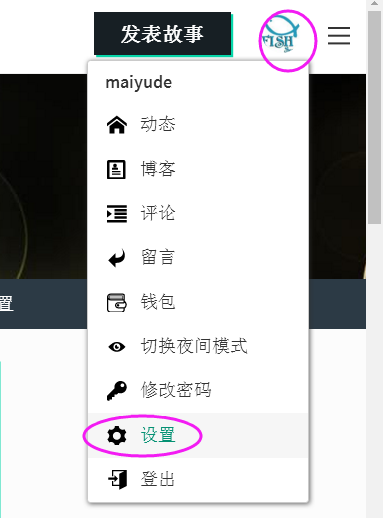
\includegraphics{images/1-1.png}

我们点击右上角自己的头像,然后点击设置,即可进入设置界面。

下面我们来根据下图一步步讲解所有设置的作用。

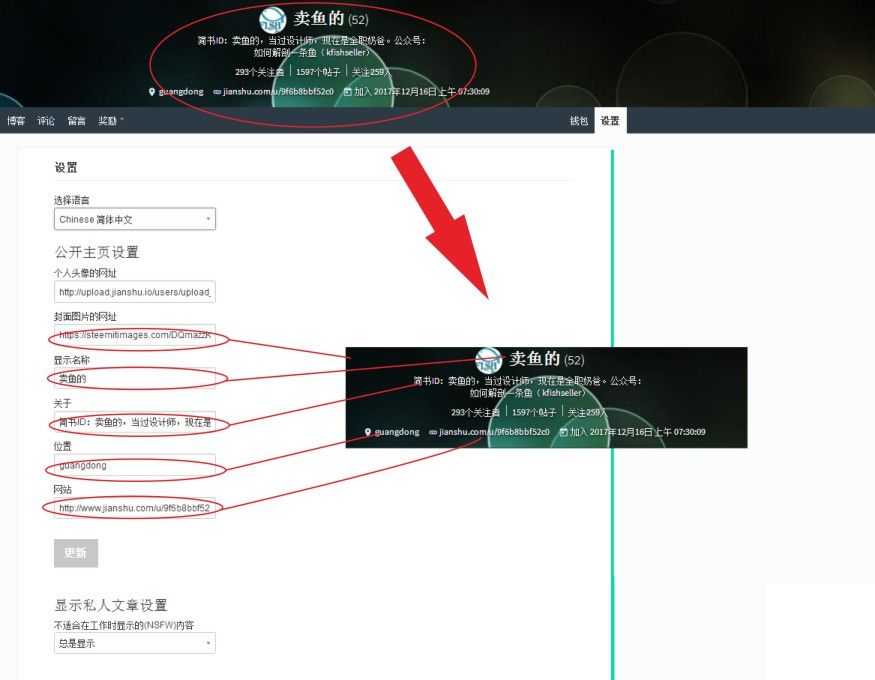
\includegraphics{images/1-2.jpg}

\begin{itemize}
\item
  1.选择语言:这里可以设置Steemit的语言,请根据自己习惯使用的语言选择。
\item
  2.个人头像的网址:这里是设置头像的地方,头像是别人对你的第一印象,设置很简单,只要把头像图片的网址复制上去即可。这里建议可以新建一个帖子,把你头像的图片上传,再把网址复制过来即可。
\item
  3.封面图片的网址:这里是封面图片设置的地方,如同箭头所示,是你主页头部标题栏的背景图片。为了各种分辨率以及各种设备都能正确显示,建议使用图片大小为1900*200 px。
\end{itemize}

设计封面图片的注意如下:


\includegraphics{images/1-3.jpg}

图中绿色区域为自由区域,红色区域为文字显示区域。

请设计图片的时候不要使用太花俏的背景,以免文字显示效果差。文字区域文字颜色为白色,所以红色区域在设计的时候注意不要使用白色背景,这样文字会看不见。

\begin{itemize}
\item
  4.显示名称:显示在你主页上的名称,不同于ID,这里支持任何语言包括中文。
\item
  5.关于:这里是你的个人简介,请简明扼要的介绍你自己。
\item
  6.位置:这里填写你的坐标,方便同区域的朋友找到你。
\item
  7.网站:这里可以填写你的个人主页的地址。
\item
  8.显示私人文章设置:不适合在工作时显示的(NSFW)内容。在Steemit,带有色情、暴力等儿童不宜的内容会打上NSFW,默认是隐藏的,你可以在这里自由的设置显示还是隐藏。
\end{itemize}

以上就是设置界面的全部内容,接着我们介绍钱包界面,点击进入钱包后,我们会看到这样的界面,下面我们来逐一介绍。

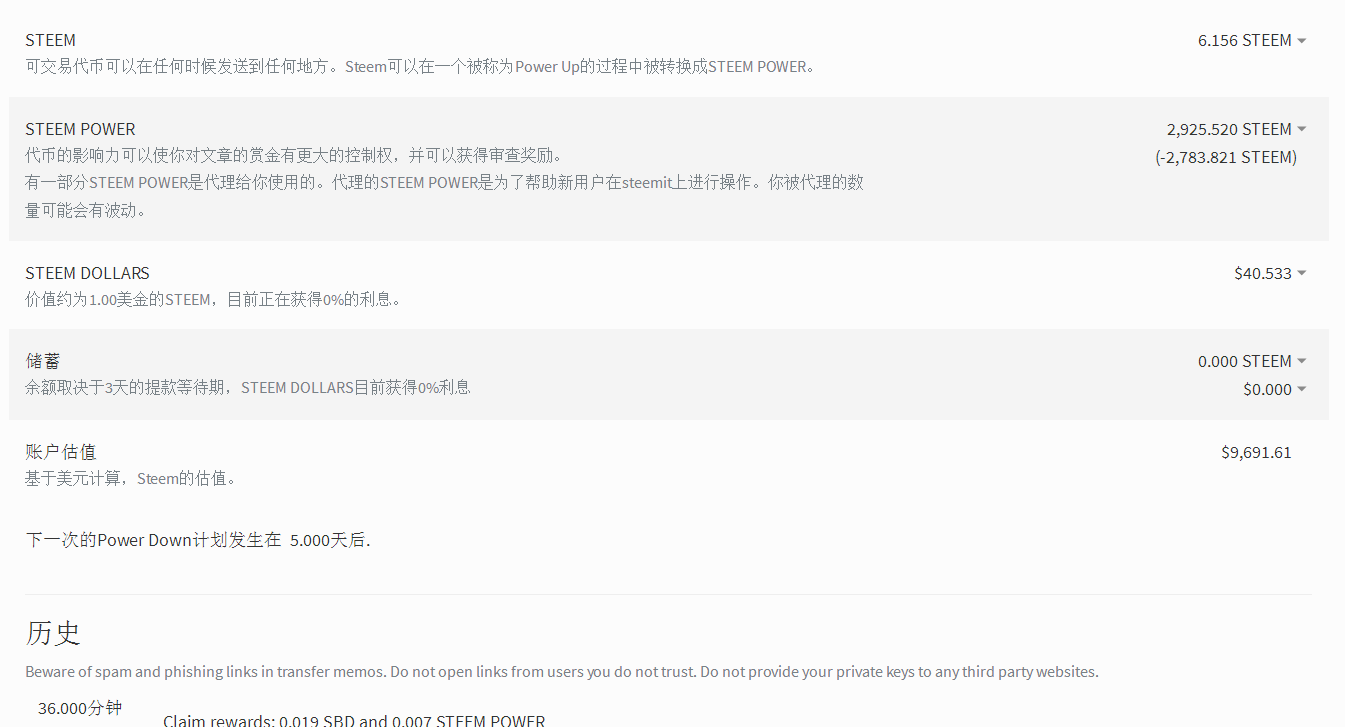
\includegraphics{images/1-4.png}

\begin{itemize}
\tightlist
\item
  1.STEEM:这里显示你账户steem余额,点击余额的数字会出现菜单。
\end{itemize}

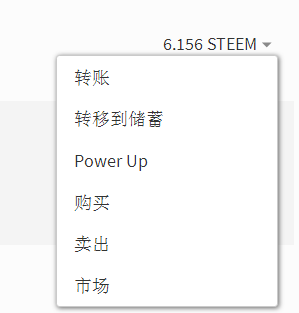
\includegraphics{images/1-5.png}

转账:转账给别的用户。

转移到储蓄:转移到储蓄账户后需要3天的时间才可以取出,一定程度保障你的资金安全。

Power Up:将Steem转化为Steem Power(SP),转换比例是1:1,转化为SP是即时的,但是SP转化为STEEM需要13周,请谨慎操作。

购买:将跳转至blocktrades,可以使用其他虚拟货币购买STEEM。

卖出:将跳转至blocktrades,可以使用将STEEM转化为其他虚拟货币。

市场:内部市场,可以进行SBD和STEEM的买卖。

\begin{itemize}
\tightlist
\item
  2.STEEM POWER:右侧数字为你的SP的数量,括号内的数字为代理的SP数量,关于代理详见后文 关于SP代理的一切一文。此处数字为2925.520,括号为2783.821,意思为总SP数量为2925.520,代理给别人的数量为2783.821,既实际SP数量为2925.520-2783.821=141.699。同样点击数字会跳出菜单。
\end{itemize}

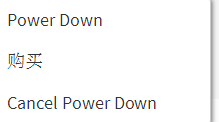
\includegraphics{images/1-6.png}

Power Down:将SP转化为STEEM的选项,全部转化需要13周的时间,Power Down期间SP的投票权不会丧失。

购买:将跳转至blocktrades,可以使用其他虚拟货币购买SP。

Cancel Power Down:点击Power Down后才会出现的选项,可以随时取消Power Down。如果你没有进行Power Down但是出现此选项,请注意你的账号密码是否已经泄露。

\begin{itemize}
\item
  3.STEEM DOLLARS:显示你STEEM DOLLARS(SBD)余额的地方,点击数字后同样会出现菜单,选项功能同上文所述,不再重复。
\item
  4.储蓄:可以将steem或者SBD转移到此处,储蓄取出需要3天的时间。把多余的钱存在储蓄可以一定程度上保障你的资金安全,因为某些原因,储蓄几乎没有利息。
\item
  5.账户估值:你的账户所有STEEM和SBD的总价值估计。
\end{itemize}

下面界面为账户的资金往来历史,如果有异常的转账行为,可能是你的账号已经泄露,请注意安全。

接下来介绍下一个界面:权限

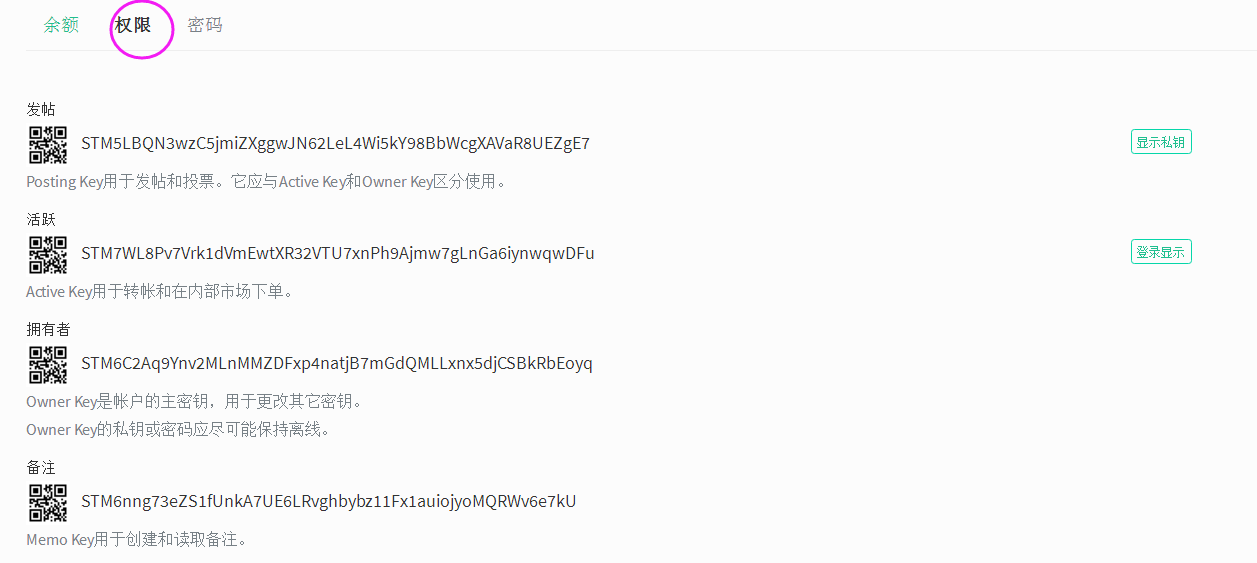
\includegraphics{images/1-7.png}

此处显示你账号的4种密码,具体作用功能描述请看后文:关于密码的一切。

最后点击剩下的最后一个界面:密码

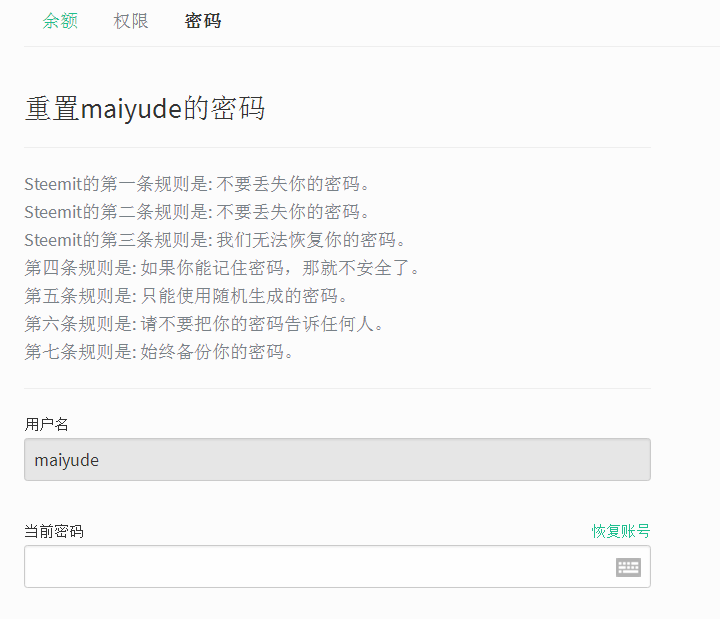
\includegraphics{images/1-8.png}

此处是修改密码的界面,不过多阐述,但是请注意修改密码前后牢记密码,修改前后的密码都要牢记。

全部界面介绍完毕,祝你的Steemit之旅愉快。

\section[第一帖 ]{\texorpdfstring{第一帖 \footnote{作者:@oflyhigh;小故事:@maiyude;编辑:@maiyude;原文链接:\url{https://steemit.com/steemit/@oflyhigh/steemit-and}}}{第一帖 }}

小雅准备在steemit写自己的第一篇文章。

她点击了发帖的按钮,之后弹出来的界面让小雅有点惊讶。这是她见过最简陋和功能最少的界面,整个界面几乎全是空白,她想找个插入图片的按钮都找不到,更别说调整字体大小等功能了。

应该是自己不懂用法而已,慢慢摸索吧。小雅心里这么想着,决定日后再一步步探索各种功能,现在首先考虑第一帖写点什么。

不如就写个自我介绍吧?一个好点子突然从脑袋里蹦了出来。说干就干,小雅花了一个小时精修了自己的自拍照,然后认真的写了一篇简短有趣的自我介绍。

文章写完,小雅认真的检查了一遍,然后按下了``发布''的按钮,大功告成。

接下来就是等着别人给自己点赞了,会有多少人给自己点赞呢?小雅满怀期待的等待着。

\begin{center}\rule{0.5\linewidth}{\linethickness}\end{center}

当你和小雅一样,兴致冲冲的注册了steemit 账户,开启发帖赚钱之旅,是否会遇到一些小问题,比如

\begin{itemize}
\tightlist
\item
  如何发布帖子
\item
  如何编辑和排版帖子
\item
  如何插入图像
\item
  Tag 是啥,要咋写
\item
  Rewards 那地方 50\%/50\% 是什么鬼?
\item
  什么时候发奖
\item
  如何查看我的收益
\item
  为何我的收益缩水了?
\end{itemize}

为了方便新用户,我在这里统一介绍一下,如有谬误,欢迎诸位批评指正。

\subsection{如何发布帖子}

登陆steemit并点击右上角的 Submit a Story 就进入发帖界面啦
发帖界面很简单,估计不用多说啦

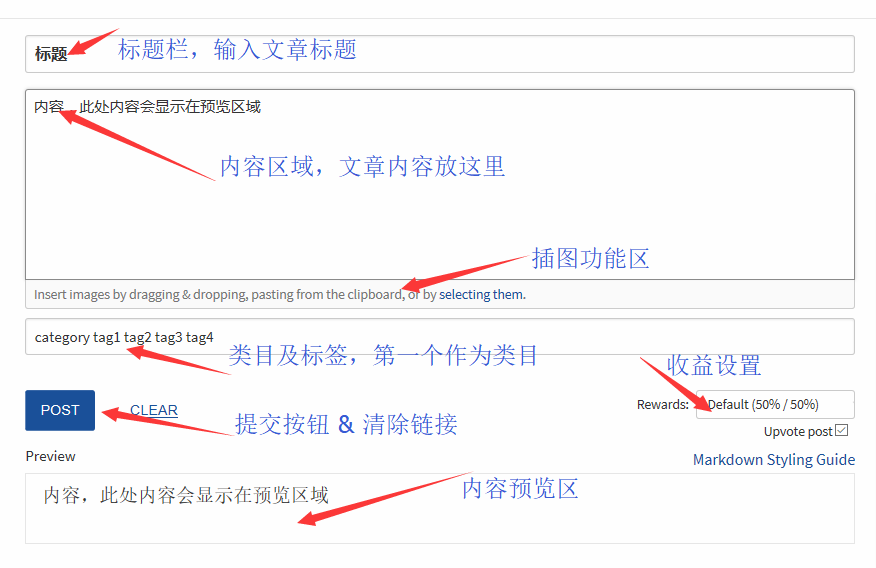
\includegraphics{images/1-5-01.png}

\subsection{如何编辑和排版帖子}

帖子有两种编辑模式,一种是Editor模式,有些类似我们使用WORD,无需多言

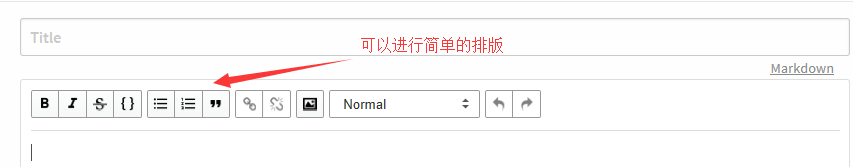
\includegraphics{images/1-5-02.png}

另外一种是MARKDOWN模式
可以参考后面关于MARKDOWN语法的使用帮助。

\subsection{如何插入图像}

插入图像可以分为 插入外部图像链接,以及插入本地图像

插入外部图像链接的方法,在后文的Markdown语法讲解中会有讲
大致就是 \texttt{!{[}图片描述{]}(图片链接)}

插入本地图像的本质,就是将本地图像上传到steemit的图像服务器,然后自动插入链接

正文区域下边的小字就是教你如何上传图像的,有三种方式

\begin{itemize}
\tightlist
\item
  1.通过拖拽操作,把图像拖到编辑框中
\item
  2.将剪切板的图像黏贴到编辑区
\item
  3.点击链接选择并上传图像
\end{itemize}

虽然原则上三种方式效果应该一样,但是我个人觉得第三种方式最好用。

\hypertarget{tag-}{%
\subsection{Tag 是啥,要咋写}\label{tag-}}

Tag是关于你帖子的标签,也可以说是类目。
其中,第一个标签是主类,也就是打开文章URL中的类目部分。

加入适合的标签,你的帖子就会出现在对应的类目下,这样更方便别人看到你的帖子,收获点赞。

Tag目前只支持英文小写字母、数字、以及一个中划线。

需要注意的是,不要为了收益去蹭不相关的类目,否则会引起别人的不愉快。
如果因此被别人差评,就得不偿失了。

\hypertarget{rewards--5050-}{%
\subsection{Rewards 那地方 50\%/50\% 是什么鬼?}\label{rewards--5050-}}

很多新人,甚至一些老人都搞不懂这个是啥
如果你懒得研究,那么用默认的 Default (50\%/50\%)就很好了。

\begin{itemize}
\tightlist
\item
  Power UP 100\%: 将文章奖励 100\% 存成 STEEM POWER
\item
  Default (50\%/50\%): 文章奖励的50\%存成 STEEM POWER,另外 50\% 已 STEEM \& SBD 组合形式发放(根据市场行情,可能是一种或者两种组合)
\item
  Decline Payout: 文章不要奖励,对应文章的所有奖励会回归奖池。
\end{itemize}

\subsection{什么时候发奖}

文章奖励会在文章发表7天以后发放。
点击文章收益右侧的小倒三角,会显示文章潜在收益以及还差多久发放。

比如下图就是我昨天一篇文章的潜在收益:

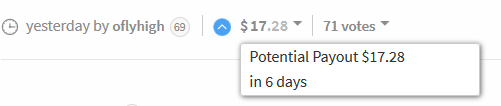
\includegraphics{images/1-5-03.png}

\subsection{如何查看我的收益}

当帖子7天发奖之后

可以通过点击右上角你的头像-\textgreater{}Wallet-\textgreater{}Rewards-\textgreater{}Author rewards
来查看你的文章收益。

或者直接访问以下链接查看:
\url{https://steemit.com/@your-id/author-rewards}
将your-id替换成你自己的steemit account

比如这是我13天之前获得的收益
\textgreater{} 13 days ago 2.198 SBD, and 1.750 STEEM POWER for oflyhigh/31

\subsection{为何我的收益缩水了?}

为何发奖前显示我的文章100 SBD, 发奖后我才得到70 多SBD ?
文章发奖前显示的收益,包括作者收益以及点赞者的点赞收益
而发奖时,点赞收益发给了点赞者,所以作者得到的收益就会少于之前显示的金额。

\hypertarget{steem}{%
\section[steem的魅力 ]{\texorpdfstring{steem的魅力 \footnote{作者:@incrediblesnow;编辑:@maiyude;原文链接:\url{https://steemit.com/cn/@incrediblesnow/jklx2-steemit}}}{steem的魅力 }}\label{steem}}

欢迎有着无限想象力与创造力的你, 到Steemit创作吧!

此篇帖子是专门为``你''而写 - 无论是正在上网、博客、艺术家、教育家、设计师或纯粹对加密币好奇的你。

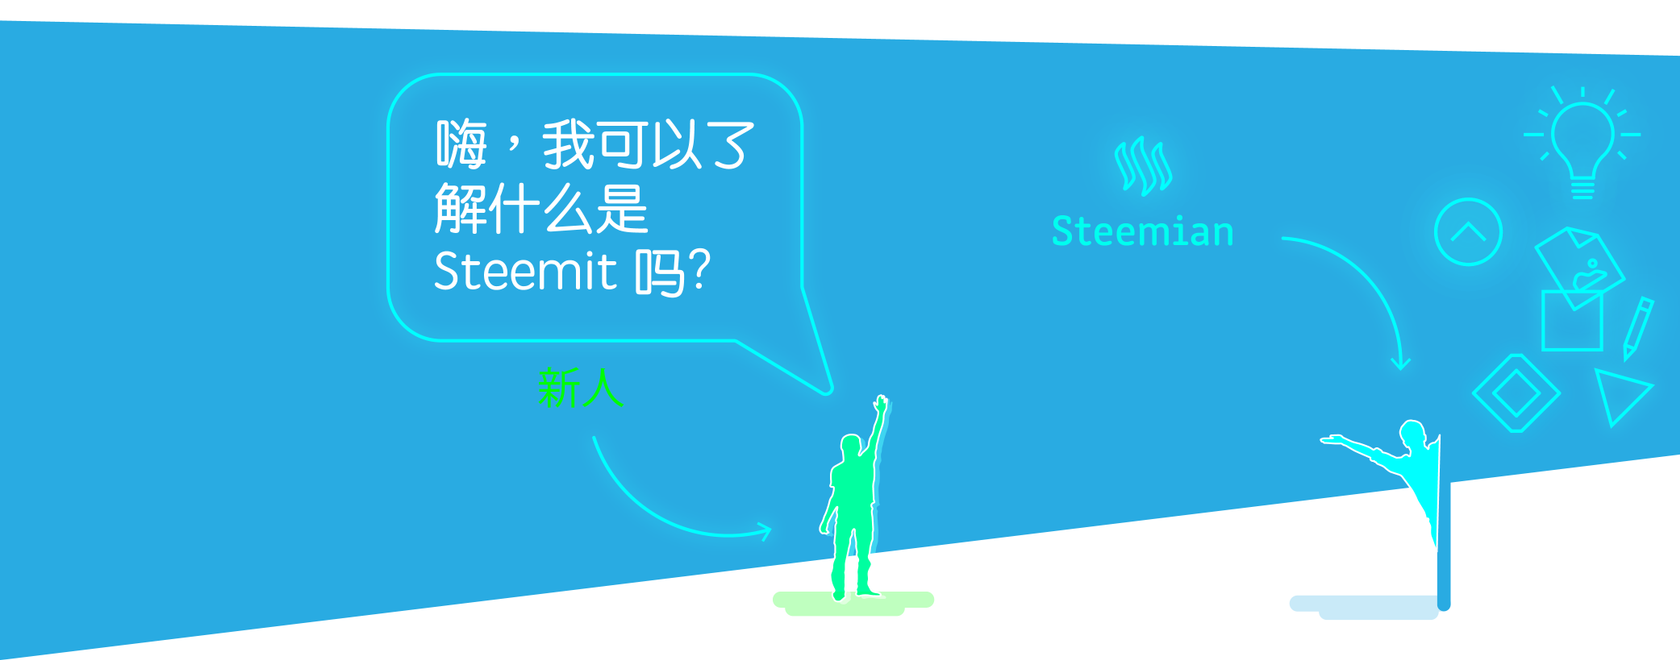
\includegraphics{images/01-06-01.png}

\textbf{Steemit,一个全新的社交网站}

从外观看来, Steemit.com 确实很像 Reddit.com,因为在 Steemit的主页上有``trending''这个按钮,当我们点击``trending''以后,就会看到很多受欢迎的帖子。不止如此,Steemit 上也与 Reddit 极为相似之处就是 Steemit 上也有个人简介页面、帖子动态、追随者等等\ldots{}. 然而,Steemit有一个与其他的社交网站迥然不同之处,那就是在 Steemit上,我们会给予用户奖励,当他们分享些有创意和有价值的内容。在 Steemit 上,当有用户认同你的创作并赞(或称upvotes),你就会得到一定的奖励。值得注意的是,每一个赞都是有着真正的金钱价值。在每一天,你只要创作、或在其他用户帖子下留言,你都有着被奖励的可能性。

\textbf{有趣化地使用社交媒体}

你的点赞与参与能增加一个帖子的奖励!如果你喜欢某某人所分享的帖子,你可以按 `赞' 来来表达你对帖子的认同。这个 ``赞'' 的功能与脸书上的 ``赞'' 的功能是完全一样的,唯一不同之处就是,你的赞 = 打赏。

当你点赞时,不会花费你的一分一毫、或者让你损失任何金钱损失。在 Steemit 上,我们就是要有趣化地使用社交媒体!

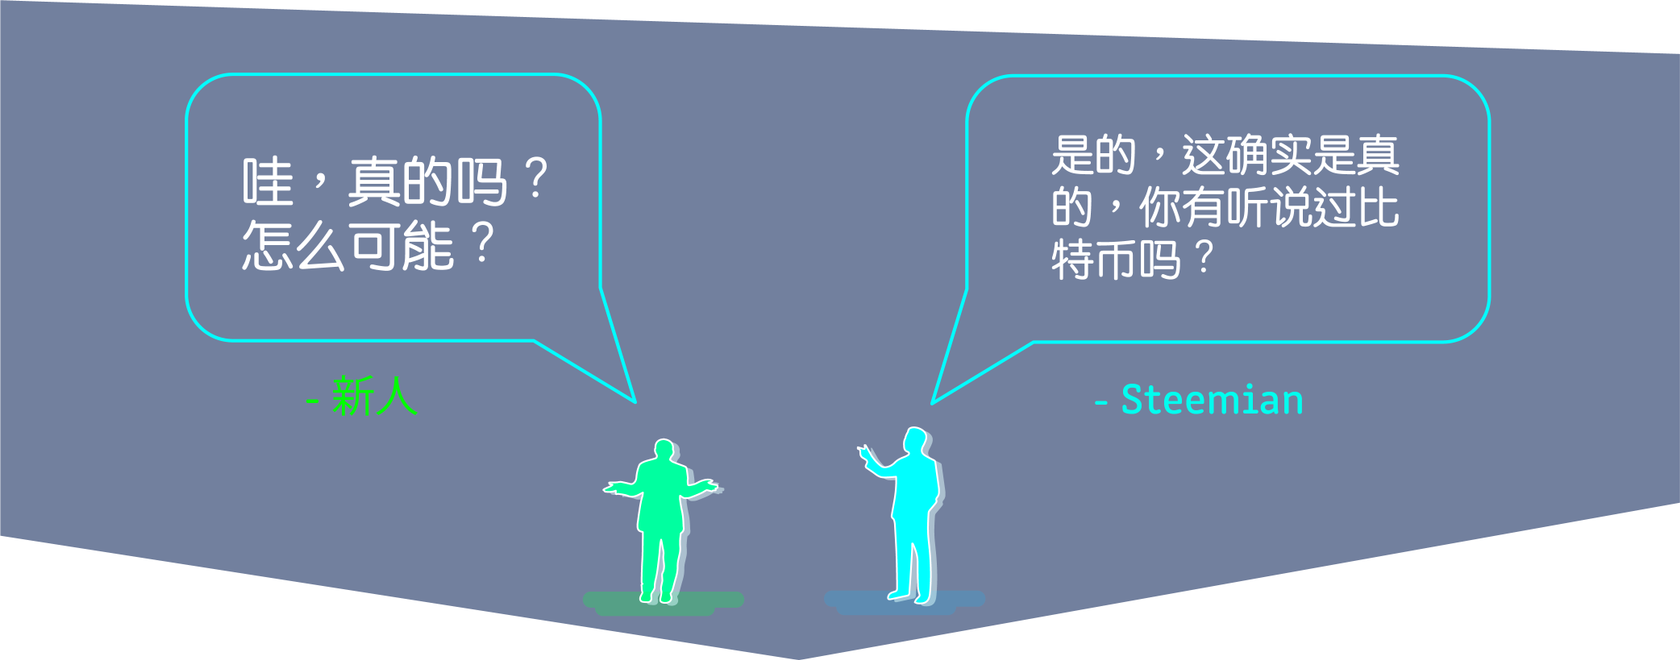
\includegraphics{images/01-06-02.png}

Steemit.com 是使用与Bitcoin 一样的科技来运行。虽然 Steemit 使用同样技术,但是Steemit 发行自己的货币,Steem(类似于比特币,都是种虚拟币。)

Steem和 Bitcoin 都是通过称为``区块链''的数据共享技术来运行。你可能已经听过``区块链''这词在一些新闻上出现,并与一些大公司牵扯上,就好像 Microsoft 公司、Blackrock 或 IBM。对这些大公司来说,区块链是令人兴奋的新技术,因为这项技术能够非常快速地运转,并且安全度极高,并能可以智能地分享数据。令人好奇的是,在区块链 到底有运行得多快速呢?打个比方,我们把支票存入银行都必须3至5个工作日才能出现该笔款项。然而区块链,这个过程能在几秒内完成。

保守估计,在未来几年,区块链技术将会颠覆社交媒体的原本风格,因为它不止改变了分享数据的方式,而且它还能够非常安全和快速的在全球共享资料。


\includegraphics{images/01-06-03.png}

每一天,Steemit 网站会发放一笔奖金在自己的网站上。所以,当你发文章时,你就会根据你所得到赞的百分比来分配那一笔奖金(和当天所有发文的用户瓜分)。

\textbf{Steem 钱币价值何在?}

与比特币一样,你可以在任何虚拟币交易所上进行交易Steem。在2018年3月27日,Steem 的价值是1 Steem 值 \$1.75美元或¥11人民币。

与比特币不同之处则为,Steem的价值不止会根据市场的需求和供应来定价,Steemit 上的内容和功能更新都会影响到币价。举个例子,当Steemit 创始人, \citet{ned} 开区了一项新的项目发展,SMT(Smart Media Token)时,Steem 钱币就暴涨了 50\%,因为这一项消息是振奋人心并且让投资者看到很光明的未来,所以Steem 的价格就水涨船高了。简单来说, Steem 钱币的币值跟股票一样性质,不止会根据市场需求变动,还会跟着新消息或 Steemit 更新而浮动。

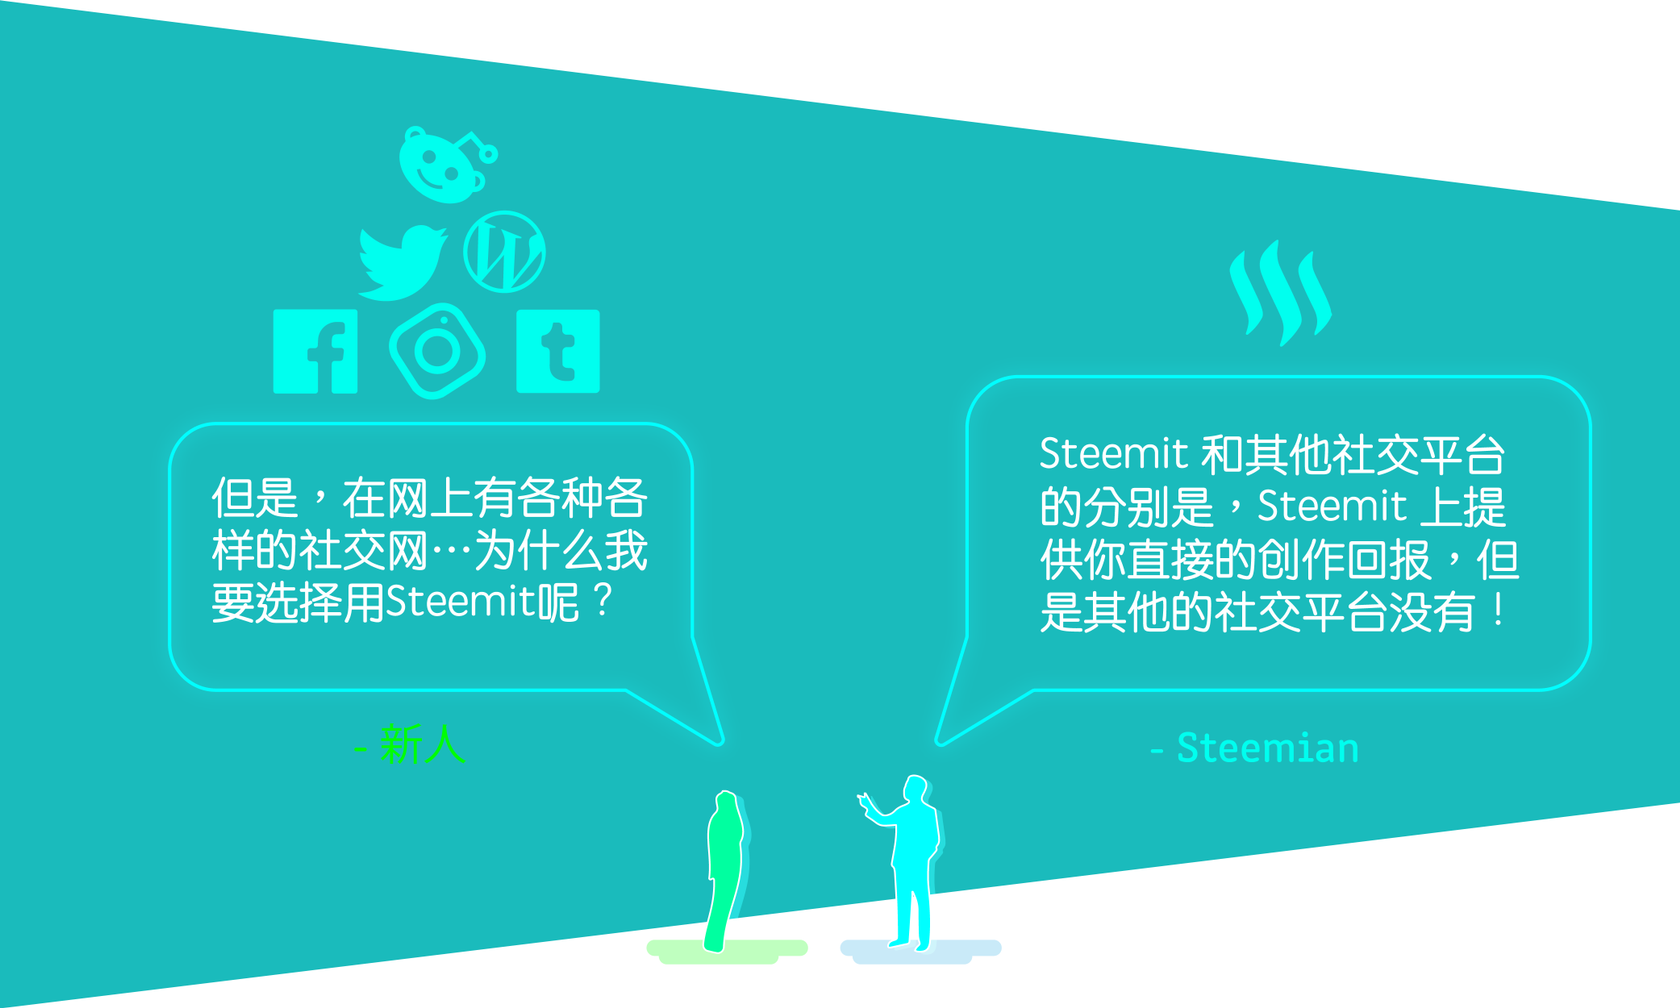
\includegraphics{images/01-06-04.png}

\textbf{Content is valuable!}

你每一天都在各个社交平台上发帖,但是你有没想过其实,你其实就是在为这些社交平台免费打工?为何出此言?当你发帖时,你就会吸引你的追随者和朋友阅读你的帖子,无形中,你就是在为社交平台引流量来观看你帖子旁的广告。但是,请问这些社交平台有没有分一些收益给你作为回报?

没有!他们连一分一毫都不愿分享给你。但是, Steemit.com 作为全新的社交平台愿意与你共享收益!在 Steemit 上,只要你分享有价值和精彩的帖子,我们都愿意跟你共享收益(我们严厉拒绝发水文的用户!)。这是我们 Steemit 非常骄傲之处,所以,我们在此非常希望你的加入!


\includegraphics{images/01-06-05.png}

当Steemit 平台成立几个月时,我们有在主页设置一个横幅,我们自称Steemit为``互联网第一个小城镇'',为什么呢?因为在这里,我们会像小镇上的村民一样,非常友善地互相对待对方。在这儿,我们不鼓励极端言论,而是鼓励努力创作。所以,我们身为 Steemians,非常希望这个社交平台能够成功!虽然这只是个全新的实验和全新的经济模式,但是我们希望 Steemit能够成为社交平台里的一股清流!

在Steemit 上,你不止可以与你认识的人交流,就如高中朋友,邻居或同事。 在Steemit,我们能够让你找到志同道合、相同兴趣和想法的人,并鼓励你与他们接触和交流,扩展朋友圈!此外,建设性的评论也将获得额外奖励,这也是我们引以为傲之处! Steemit一定是是第一个具有奖励性的社交媒体平台!

这是我们邀请你加入Steemit最主要原因,因为我们希望你成为我们未来的一部分。我们需要你独特的世界观、才华和热忱,为Steemit建立更强大的未来。


\includegraphics{images/01-06-06.png}

欢迎加入Steemit 大家庭!
心动了吗?那么还不赶紧注册?Steemit 是完全免费加入!

点击\href{https://steemit.com/pick_account}{注册},等待2-4 天,就能够得到帐号了。
然后记得发一篇帖子进行自我介绍,让我们了解你!


\includegraphics{images/01-06-07.png}

\hypertarget{-steem}{%
\section[一分钟入门 steem ]{\texorpdfstring{一分钟入门 steem \footnote{作者:@dapeng,原文链接:\url{https://steemit.com/cn/@dapeng/steem-or-the-very-first-post-for-new-steemians-to-read}}}{一分钟入门 steem }}\label{-steem}}

很多新人来到 steem,满脑子问号,提了一堆问题,花了很多工夫,却仍然没能入门。

向新人介绍 steem 的好帖有很多,在 steemr.org 上有总结,这里不重复。其中最简单粗暴的,我认为是 @jubi 最近写的 \href{https://steemit.com/cn/@jubi/28tqtu}{``写与我的一些自媒体朋友''}。我喜欢这篇文章的调调,例如:

\begin{quote}
钱从哪儿来?这个问题说实话,我不想回答。知道又如何,不知道又如何。
\end{quote}

该文的作者,一定曾经受伤很深。

一个新兵蛋子,刚来就问连长的老婆是从哪里讨来的,这不合适吧?

不过,就算是这篇通俗得已经不能更通俗的帖子,仍然有很多新人读完后搞不明白,毕竟里面提到了一些新概念。

通过观察,我发现,纠结的根本原因是,新人们没闹明白 steem 是什么。弄清楚了这个问题,其他问题都迎刃而解。

\textbf{steem 到底是什么?}

steem 不是个摇钱树啊!你来了,摇一下,就有金币砸你的脑袋!(除非你先把金币挂上去------这句话的意思你将来会懂,现在解释了也没用。)

steem 也不是提款机啊!你塞进去个账号,就吐出一叠美钞!(除非你预存进去------这句话的意思你将来会懂,现在解释了也没用。)

我用大白话解释一下:steem 是个圈子。

steem 好比现实生活里的一群人,围坐成一圈开篝火晚会。(steem 网站)

篝火旁边可以表演节目。表演完了有人发钱。(发帖赚钱)

篝火有好几堆。这一堆附近全是说中文的,那一堆附近全是画家。中国画家两堆来回跑。(分区)

晚会上有人载歌载舞,有人冷冷旁观,时不时有人抽身离去。(活跃账号,休眠账号,死账号)

有些人,幕后是同一个老板,组团来表演;有些人,其实是人工智能的机器人。(马甲,小号,机器人账号)

作为一个新人,你来到这个晚会现场该怎么做,你在 steem 上就该怎么做。

你不能上来就伸手,问晚会现场每个人要钱,对吧?(快来点赞我吧)

你不能挨个问现场的每个人,喂,你兜里有多少钱,对吧?(到底 steem 上能赚多少钱)

你不能易容改装成鹿晗,说自己是正牌大明星,把大家当傻子,对吧?(steem 上能不能抄袭)

拜托,\textbf{正常一点}好吗?

一个正常人,来到篝火晚会,首先应该找个角落先坐下,适当的时候站出来,做个自我介绍,最好彬彬有礼,说说自己是谁,兴趣爱好什么的,别人才方便跟你交朋友(写个自我介绍帖)。

不爱说话,那就点个头,坐在角落默默围观,等有人来好奇地问你你是谁你来做什么(等着别人来你的帖子回复,互访,互动)。

遇到现场放你喜欢的音乐时,趁机上去跳个舞,震震他们(参加 steem 上举办的各类活动,写自己擅长的内容)。

为什么有人表演得到的钱多,有人表演得更好却得钱少?坐下来看,自己慢慢找答案。(读前辈的帖子)

为什么我表演了也没人给我发钱?你得认识能发钱的人啊。他们要是不知道你是谁,凭什么给你发钱?(新人发帖赚钱少)

这就是 steem 的一切。

\textbf{新手要做的事情,就是当个篝火晚会现场的正常人。仅此而已。}

新手在 steem 上无所适从的时候,就想象自己是在一个篝火晚会现场,遇到这种情况怎么办。你会发现,问题迎刃而解。

``steem 是什么''这个问题解决之后,应该不会存在什么观念上的疑惑了。剩下的就是几个基本的技术问题。

\textbf{第一: 注册。}

上 steemit.com 直接注册,上面的提示信息很清楚:要注意什么,几天能注册下来,等等,完全不需要求助。

如果存在访问障碍或者语言障碍,那就去 cnsteem.io 注册,也不需要求助。不就是十块钱的事儿嘛。cnsteem.io 的主人是 \citet{skenan},有问题联系他发邮件到 \href{mailto:cnsteem@gmail.com}{\nolinkurl{cnsteem@gmail.com}}。

\textbf{第二:访问速度慢。}

改用 cnsteem.com (中文界面)。或者 busy.org。内容跟 steemit.com 完全一样。没账号的人可以浏览。有账号的人可以用 steemit 账号的 post key 登录发帖。

\textbf{第三:其他问题。}

steem 网站顶部都有搜索栏。输入关键词,自己搜。google 百度上搜也行。

系统性阅读的话,可以参考:\href{http://steemr.org}{steemr.org}(嫌慢就去 \href{http://steemit.wang}{steemit.wang})

以上涵盖了新人遇到的所有问题,除此之外,再无废话。

\hypertarget{change-color}{%
\section[更改 steemit 的网页界面配色 ]{\texorpdfstring{更改 steemit 的网页界面配色 \footnote{作者:@dapeng,原文链接:\url{https://steemit.com/steemit/@dapeng/if-you-dislike-the-steemit-green-or}}}{更改 steemit 的网页界面配色 }}\label{change-color}}

你喜欢 steemit 的新界面吗?尤其是那一片绿\ldots{}\ldots{}

如果不喜欢,本文告诉你如何方便快捷地更改。目前的主流浏览器都支持更改网页的默认颜色。本文就以 Firefox 为例,给出三种方法,任你选。

方法 1:点击 firefox 右上角三条小横线按钮,点击``选项'' --- ``内容'' --- ``颜色'' ---``覆盖''下面选永远。

这种方法的好处是啥都不用额外安装。坏处是所有网站都变成了你指定的颜色,想切换回去的话又得点一遍。有没有办法一键切换?

方法 2:在``选项''里点``插件'',搜索 ``No Color''插件。安装完毕后,工具栏多出个按钮。点它,就可以一键在你定义的颜色跟网站原来的颜色之间切换了。

虽然切换方便,但是有没有办法不切换,自动把且仅把 steemit 颜色改了?

方法3:安装 `NoSquint Plus' 插件,工具栏又多个按钮。点它,设置颜色。``全局选项''可以选择对所有网站都改颜色。如果只对 steemit 改,那么把'排除`'勾上就行了。

\hypertarget{jbcsp_}{%
\chapter{基本常识}\label{jbcsp_}}

\hypertarget{what-is-steem}{%
\section[什么是 steem]{\texorpdfstring{什么是 steem\footnote{作者:@wang-peilin;小故事:@maiyude;编辑:@dapeng}}{什么是 steem}}\label{what-is-steem}}

小雅的第一篇文章发出去之后,只有寥寥几个人给她点了赞,收益也只有可怜的0.03美元,这让她有点失望。

不过她很快就从失落中走了出来,自己还只是个新人嘛,没人关注是很正常的事情,加油写文章就是。

小雅开始翻看steem官网的介绍,不过越看介绍小雅就越是迷糊。这里有个叫steem区块链的东西,又有一个叫steemit的网站,还有一个叫steem的货币,而且还夹杂着各种各样的专业名词,看的小雅头疼不已。

终于,小雅决定放弃了解什么是steem,专心写文章去了。

\begin{center}\rule{0.5\linewidth}{\linethickness}\end{center}

面对steem各种繁复的设定,相信很多人都会和小雅一样一脸的困惑,下面就来简单的介绍一下什么是steem。

\begin{itemize}
\tightlist
\item
  1.前言
\end{itemize}

什么是Steem?新人朋友们看到这个标题可能会有点摸不着头脑,Steem不就是在Steemit.com上使用的一种货币吗,还用单独列一个章节出来讲解?会这样想主要是存在一定的误区,因为Steem其实有两个含义,一个是Steem区块链,另一个则是在这个区块链上使用的一种货币。为了方便区分,我们暂且把第一个含义叫做Steem链,第二个含义叫做Steem币吧。而我们大多数朋友都是通过Steemit.com上最先接触到Steem链的,所以我们下面单独讲解一下Steemit.com吧。

\begin{itemize}
\tightlist
\item
  2.Steemit.com
\end{itemize}

Steemit.com是由Steem区块链的官方开发者建立的一个网站,在这个网站上我们可以读取到Steem链的内容。在Steemit.com上我们使用Steem币来奖励那些发布文章或点赞文章,以及发布图片和评论的用户。和博客、QQ空间、微信类似,用户可以发贴,评论。不一样的是,Steemit会给你奖励,激励你发布更多更好的文章。Steemit.com也是想最终发展成一个聚集时尚、经典、阅读、热点和流行的平台。

\begin{itemize}
\tightlist
\item
  3.其它接入Steem链的网站
\end{itemize}

除了Steemit.com外,我们还可以通过Busy、eSteem、ChainBB、Utopian.io、Steepshot、Zappl、DTube、Dsound、Dlive、Dmania等各类网站输出或输入Steem链上的内容。就好像以前我们使用的光盘,我们不仅能在DVD上播放光盘的内容,还可以在EVD甚至有光驱的电脑上播放这个光盘。最重要的内容就存在这小小的光盘上。那么我们要问这么神奇的Steem链,究竟是什么呢?

\begin{itemize}
\tightlist
\item
  4.Steem链的本质
\end{itemize}

Steem区块链采用的是跟Bitshares一样的石墨烯(Graphene)区块链技术,其共识模式是DPoS,Delegated Proof of Stake,大致上说,就是由持股者按持股比例投票选出代表(Witnesses)来维护、验证区块链网路 ( 简单对照比特币是PoW,藉由算力来决定共识之产生)。

区块链很多,甚至DPoS类型的也有一些,重点在于Steem链的特色是什么?你可能说是内容链平台。这么说也没有错。帮你更精确地说,是内容上链,持股者按照权重,可以决定按照机制设计好的新增代币,要如何分配到各见证人(Witnesses)、持股者(SP holders)、内容创造者(authors)以及内容发现者(curators)身上。当然,大部分是分配给内容创造者的。新增代币分给后二者部分称为奖励池(Reward Pool),目前是累积七天,动态发给,各持股者以vote形式(正负两种)来进行权重投票,七天后结算。

虽然Steem链是机器无感的,但在上面运行的东西是活的,是被人赋予意义的。我们可以说Steem链是一切的根本,是Steem世界万物之依归。而我们来自世界各地的广大用户则依托Steem链,创造了缤纷的Steem世界。

\hypertarget{gzhb}{%
\section[Steem上的各种货币]{\texorpdfstring{Steem上的各种货币\footnote{作者:@wang-peilin;小故事:@maiyude;编辑:@dapeng。本文部分引用自@rivalhw的文章}}{Steem上的各种货币}}\label{gzhb}}

小雅对文章的收益热情非常高,虽然她的钱包里面并没有钱。

小雅最近开始研究steemit里面的各种钱。她发现这里居然同时存在三种钱,分别是steem,steem power(sp),Steem Dollars(SBD)。为什么一个社区内会同时存在三种钱啊?这让小雅很是困惑,这就感觉像是市场上同时流通三种人民币的感觉,初次接触区块链的小雅完全搞不懂。

不过让小雅感到更为困扰的事情是,自己所有的钱币都是0,这让小雅顿时失去了研究这些货币的兴趣,默默的继续写文章去了。

\begin{center}\rule{0.5\linewidth}{\linethickness}\end{center}

可能很多新人会和小雅一样,对steem里面的各种货币感到混乱和头疼,就让我们一起来认识一下steem里面的各种货币吧!

\subsection{概述}

在Steem区块链上我们使用3种货币,Steem,SBD(Steem Dollars),SP(Steem Power)\textbf{(注:严格意义上讲SP不能算作一种货币,因为它不能随意流通和交易,这里把它归为货币主要是为了方便理解,具体请见下文SP的单独讲解)}。为什么一个区块链上要使用三种不同的货币呢?这主要是因为它们被赋予不同的权利,拥有不同的功能,下面我们依次介绍。

\hypertarget{steem-1}{%
\subsection{Steem}\label{steem-1}}

Steem是Steem区块链上的基础货币,另外两种币都跟它相关。你可以通过在Steemit.com,cnsteem.com等网站上通过写文章,评论或点赞来获得它。你可以在任何时间存入,取出或者与其它持有者交易Steem。Steem可以通过一个叫Power up的过程转化为SP(Steem Power)。

\hypertarget{spsteem-power}{%
\subsection{SP(Steem Power)}\label{spsteem-power}}

如上文所述,SP是Steem通过Power up的过程获得的。顾名思义,你的SP越多,你在Steem社区上的影响力就越大,你的SP越大你的点赞就越可以得到更大的收益。具体来说,按本文编辑时的实时行情,如果你有10000SP,那你的一个点赞最多可以产生 \$2.8 左右的收益。而实际收益其实远大于显示收益,显示为 \$2.8 的收益实际上大概相当于7.7美元(具体原因请看下面SP的介绍)。那既然SP这么有用,为什么不把Steem全部转为SP呢?这是因为SP缺乏流动性,不能随意取现及交易。如果我们想把SP卖掉,则需要进行一个Power Down的过程,将SP转化为Steem再进行交易。而整个Power Down的过程每周只能将你持有的13分之1的SP转化为Steem,所以当您有了一些Steem后,还是要具体情况具体分析要把自己多少比例的Steem转化为SP。

\hypertarget{sbdsteem-dollars}{%
\subsection{SBD(Steem Dollars)}\label{sbdsteem-dollars}}

SBD初衷是设计来1:1兑换美元的,官方现在也是把1SBD固定视为1美元的。但实际上它的市场价格却是像Steem一样波动的,现在1SBD的市场价远大于1美元。这也造成了文章作者获得的实际收益远大于显示收益。以上文所说显示收益 \$2.8 为例,实际收益为1.4个SBD和价值为1.4美元的SP,而按本文编辑时的市场价格,1个SBD约等于4.5美元,所以实际收益应为4.5x1.4+1.4=7.7美元。

\subsection{怎么获得这些货币}

作者在发文章之后,按照Steemit的规则,7日后文章将被锁定而且无法修改(区块链永久不可篡改性),同时进行该帖的结算,并根据作者发帖时的设定进行Steem和SBD的奖励。如果作者选择50\% 50\%,系统会将奖励分为两部分,一部分作为SBD奖励,另一部分作为SP奖励;如果作者选择发帖时power up 100\%,则系统将会将奖励全部按照SP进行power up。当然你也可以通过交易所或其它货币持有者交易来获得这些货币。

\subsection{总结}

Steem上的货币是相互依存,息息相关的,新手朋友光看这些文字可能还是不能完全理解。如果你想投资进来我建议可以先投资一小部分自己实际操作一下,完全搞清楚这里面的各种关系后再决定是否大力投资。

\hypertarget{about-sp}{%
\section{关于SP(steem power)}\label{about-sp}}

\hypertarget{sp-}{%
\subsection[SP 代理 ]{\texorpdfstring{SP 代理 \footnote{作者:@maiyude;校对:@meixia}}{SP 代理 }}\label{sp-}}

在上一节,我们学习了关于Steemit的里面几种货币的知识。我们了解到了SP(Steem Power)在Steemit的重要性。这里我们再扩展说一下SP的扩展应用------代理SP。

SP非常的重要,日常的发帖或者直接购买都可以增加你的SP。那么,当我们的SP有一定程度的富余的时候,除了点赞外,我们还有什么办法更好的使用掉这些富余的SP呢?或者我想要快速的获得更多的SP,有什么办法呢?

这个办法就是代理SP。

什么是代理SP呢?简单来说就是把你的SP借给别人使用。说到借东西给别人,很多人可能会有点忌讳,生怕有借无还,何况SP在Steemit社区那么的重要,自己用都不够呢,为什么要借给别人?

这里首先我们了解一个很多人都关心的事情,我们代理给别人的SP安全吗?

答案是非常的安全。你把SP代理给别人后,别人只拥有这些SP的使用权,但是这些SP还是安全的躺在你的钱包里面的,你可以随时的收回,不过收回的过程通常需要7天。代理SP给别人后,你的钱包界面的SP后面会有一个小括号,比如我的钱包的界面,后面显示了-2552.794STEEM,这说明我代理了2500多SP给别人。

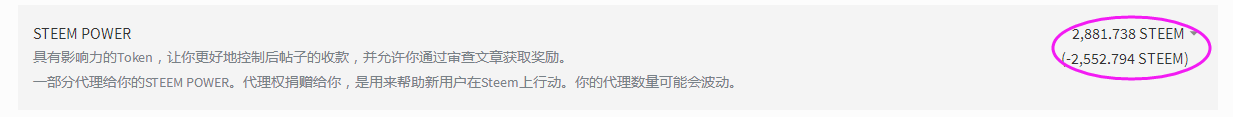
\includegraphics{images/02-1.png}

了解了最关心的安全问题后,我们又有新的疑问了。为什么我要代理SP给别人?我自己都不够用呢。

代理SP给别人主要有几个用处:

\begin{enumerate}
\def\labelenumi{\arabic{enumi}.}
\item
  代理SP给新人:代理SP给新人可以很好的帮助新人发展。比如有些应用就得到了官方的大量SP代理,这样这些第三方应用就能更好的发展了。
\item
  代理给点赞机器人等获取收益:比如代理给@justyy可以每天获得利息,代理给@cnbuddy可以获得点赞等。
\item
  出租SP给别人获取收益:出租SP在Steemit已经是一个非常常见的行为了,如果你有富余的SP,不妨可以考虑出租,这可以给你带来一定的收入。著名的租借SP服务商有:@minnowbooster等
\item
  账户资金避险:比如你可以把账户的钱分散到小号,再把SP代理给大号来分散资金风险。这样可以保证你的SP总量不变,但是SP分散到了几个账号,这样即使遇到了最坏的情况,账号被盗且无法找回,丢失的也只是一部分资金,可以减少损失。
\item
  作为奖品:可以代理一定量SP给某人作为奖品。比如我想要举办一个活动,但是目前我囊中羞涩,而且我也不太想用真金白银的SBD或者STEEM作为奖励,这时候可以用代理100个SP一个月的时间作为奖励,花掉自己未来的收益作为奖励,这或许是未来活动的一个发展方向。
\item
  暂时没想到,欢迎补充。
\end{enumerate}

可见,代理SP的作用是非常多的。比如一个新人刚来到Steemit社区的时候,如果能够获得大鲸代理的一些SP,那这位新人初期升级的速度会非常快,这对新人的帮助是非常大的。

这里着重说明一下代理给@cnbuddy或者@justyy的好处。

首先是@justyy的YY银行,只要代理SP给他,他会每天按照比例转账SBD给你。每天就算不发帖都能躺着收钱,多好的事情对吧,而且还会获得@justyy的十几个机器人群的点赞,简直是一本万利的事情。

其次是代理给@cnbuddy,代理给@cnbuddy之后,可以获得机器人给予的相当于你代理SP的好几倍的点赞。这会比你自己的点赞更加有效率并且不消耗你的Voting Power,这可以有效的提高你的收益和增快你的升级速度。如果你是一个勤于写文章的人,代理SP给@cnbuddy是一个非常好的选项。

作用都明白了,那么如果我想要代理SP给别人,应该如何操作呢?我们这里以代理SP给点赞机器人@cnbuddy为例说明。
要想代理SP给别人,需要使用@justyy开发的小工具,\href{https://helloacm.com/tools/steemit/delegate-form/}{点击这里可以跳转}

这个工具需要通过steemconnect授权,所以不用担心安全的问题。

下面介绍详细的用法,我们首先点击进入这个工具的页面。

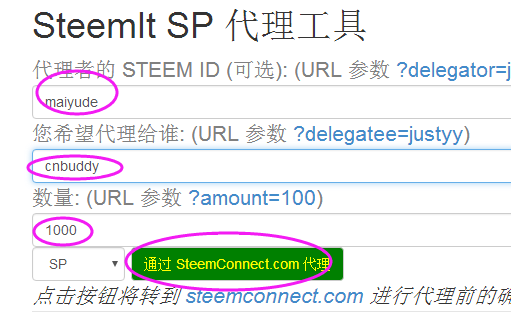
\includegraphics{images/02-2.png}

如同上图所示,第一栏填写你的ID,第二栏填写被代理者的ID,第三栏填写代理的SP数量,然后点击绿色的按钮即可。之后会跳转到steemconnect授权页面,需要你的active Key授权。

那么我要如何收回我的代理呢?只要在第三栏代理数量那输入0即可。收回需要7天的时间,这7天你无法使用你的SP。

这里再稍微介绍一下这里的SP填写规则,代理的SP以最后一次填写的为准。什么意思呢?我这里举几个实例来说明。

\begin{enumerate}
\def\labelenumi{\arabic{enumi}.}
\tightlist
\item
  我要代理1000SP给cnbuddy,那我们填写1000即可。
\item
  我已经代理1000SP给cnbuddy了,现在我要追加代理200SP过去,那现在需要填写1200而不是200。
\item
  我已经代理1000SP给cnbuddy了,现在我想要收回300SP,那现在需要填写700。收回的300SP会在7天后返回你的账户,返回的过程没什么提示,请耐心等待。
\item
  我想要收回代理的全部SP,那填写0即可,同样7天返回。
\end{enumerate}

代理操作完毕后,可能有部分人在一段时间后,会忘记了自己代理SP给过什么人,有什么办法可以查询吗?办法当然是有的,这里同样要使用到@justyy的工具,请\href{https://helloacm.com/tools/steemit/list-of-delegatees/}{点击这里跳转}

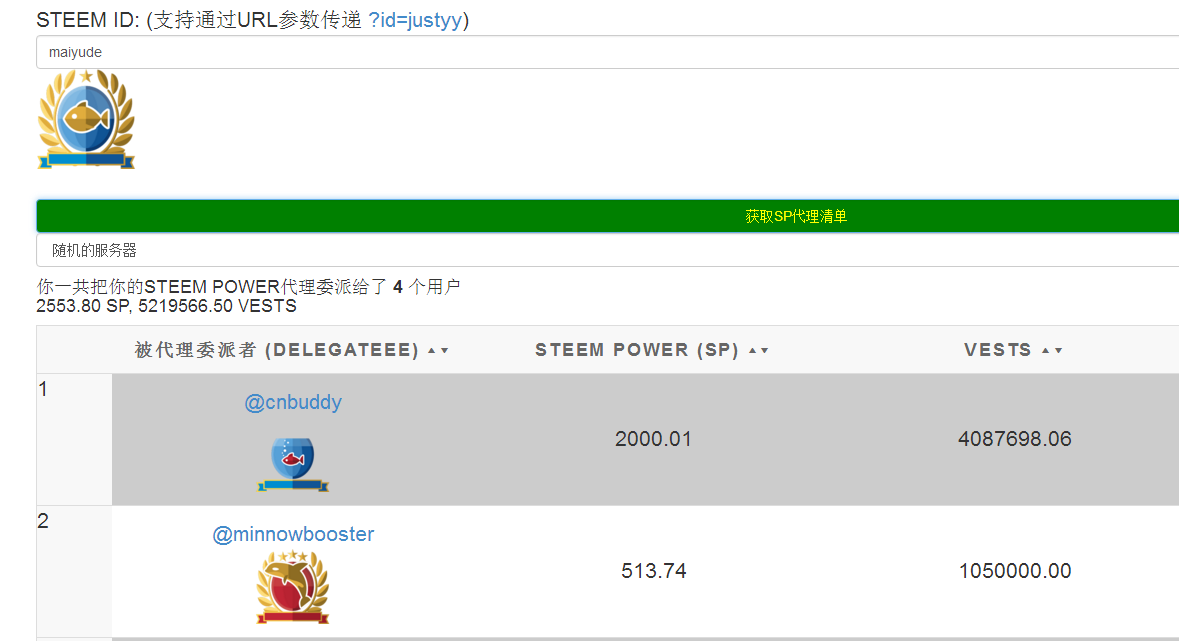
\includegraphics{images/02-3.png}

使用方法非常的简单,只要输入ID后就可以查询代理SP的清单。

@justyy的工具还可以查询谁代理了SP给你,要是哪天你发现你多了几个SP,又不知道来源,可以使用这个工具查询,\href{https://helloacm.com/tools/steemit/list-of-delegators/}{点击这里跳转}

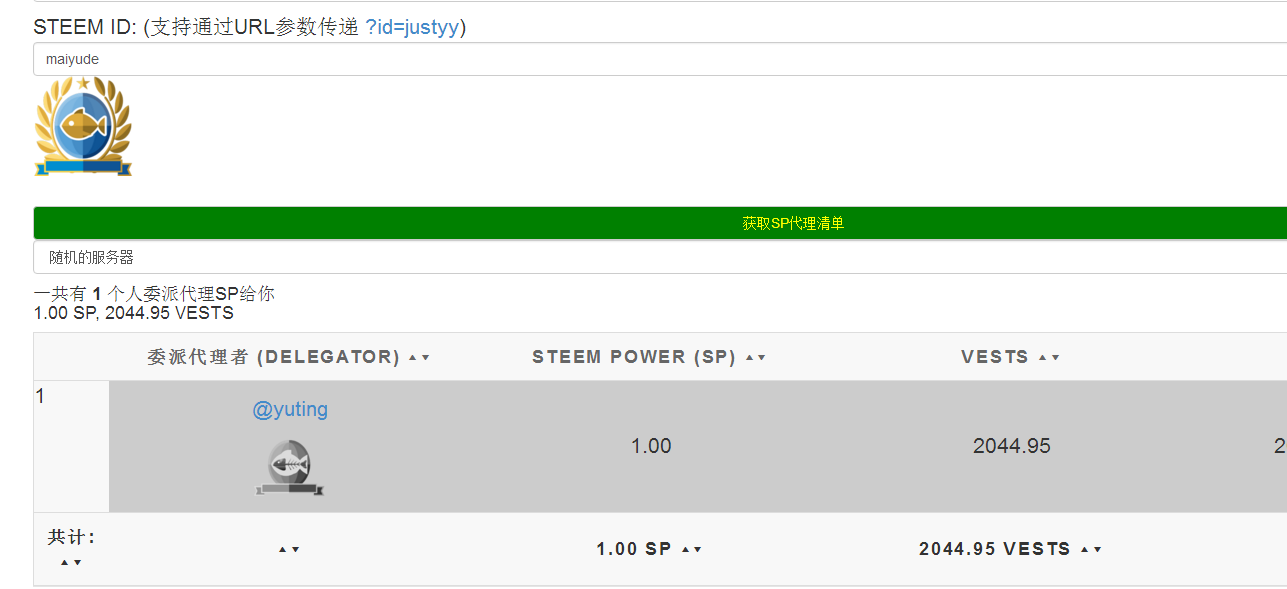
\includegraphics{images/02-4.png}

使用方法同样,输入ID即可。

总而言之,代理SP无论对自己还是对别人都是非常有用处的。所以还等什么呢?赶紧操作起来吧!

\hypertarget{power-up}{%
\subsection[power up ]{\texorpdfstring{power up \footnote{作者:@vickylin;编辑:@vickylin}}{power up }}\label{power-up}}

对于已经在steemit待了七天以上的朋友来说,理论上有第一笔作者奖励已经入账,那么我们的账户中就会有sbd。对我来说,看到价格合适的情况下就会选择用sbd买入steem再power up,大家可以根据自己的具体需要决定。

登陆主页------钱包------STEEM DOLLARS------市场
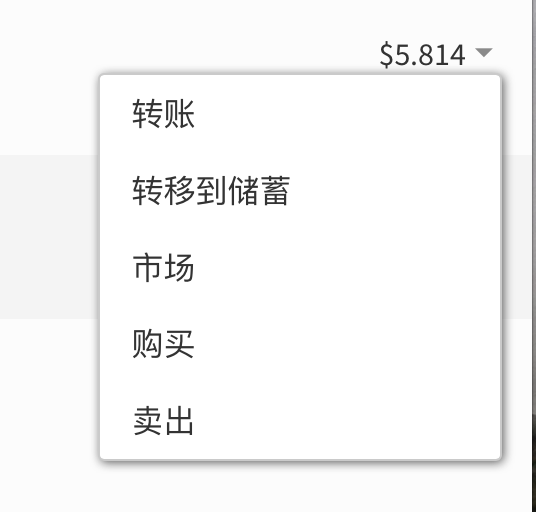
\includegraphics{images/03-power_up01.png}

进入市场后,界面如下:
\includegraphics{images/03-power_up02.png}

在左边购买steem表单中,填写入想要购买的心理价位及数量,点击购买steem;
\includegraphics{images/03-power_up03.png}

提示``确认Limit Order Create'',点击``好'';
\includegraphics{images/03-power_up04.png}

输入active key,点击登录
\includegraphics{images/03-power_up05.png}

下单成功后会在左下角提示如下:
\includegraphics{images/03-power_up06.png}

如果挂单价格合适的话,订单将会撮合成功。返回钱包,在第一栏中便可查询到刚才购入的steem;
\includegraphics{images/03-power_up07.png}

点击右侧三角形下拉箭头,选择power up,填入此次想要power up的量,按确认即可。
\includegraphics{images/03-power_up08.png}

\section[关于声望的一切]{\texorpdfstring{关于声望的一切\footnote{作者:@vickylin;小故事:@maiyude编辑:@vickylin}}{关于声望的一切}}

小雅来到Steemit已经好几天了,文章也发了好几篇了。虽然点赞的人不多,每篇文章的收益也就零点零几美元,不过小雅也很满足了,因为自己已经慢慢开始熟悉这个社区了。

小雅今天发现了一个事情,就是自己名字旁边有个括号,里面写了一个数字。她记得刚来的时候这个数字是25,今天这个数字变成了26。这让她很是好奇,她把鼠标悬停了在数字上面,屏幕显示出了一行文字``这是小雅的声望分数,信誉评分取决于收到的投票历史记录,用于隐藏低质量的内容。''

``声望?这是什么?''小雅喃喃自语道。小雅把这个理解为类似等级的东西,只要自己好好写文章,这个等级会上升的吧。但是屏幕提示的最后一句话``用于隐藏低质量的内容'',让她有点不明白,难道这里的声望会出现负数?出现了负数后账号会被隐藏吗?

看来小雅需要学习的内容还有好多。

\begin{center}\rule{0.5\linewidth}{\linethickness}\end{center}

对于新用户来说,可能会和小雅一样产生困惑,声望是什么?我们可以看到,登陆主页后名字边上的(25)就是声望,即Reputation。初始等级为25级,如果用户一些错误行为(比如:剽窃、伪原创等)或者有人恶意踩踏(downvote),会导致声望掉到0级甚至数值为负。

打个比方,声望相当于是你在steemit求学路上的一个结业证书,到达一个程度就发给你个证明。但这个证书,和你以后赚大钱关系不是很大(当然,有些机器人会偏爱声望高的用户给予点赞)。

一般来说,声望数值比作者声望数值低,踩没有影响。简单来说,一个25级的踩(downvote)30级的没有影响,而一个60级的踩55级的就会有影响。

对于新人来说,25-30级的时候升级的非常快。正常的互动下,一般一周内就可以达到。如果被大鲸点赞,甚至可以一下子到30级,但50级以后升级会非常慢。

在写这篇文章的时候,我找了很多过去前辈写过的关于该块内容的文章,看到以下这句:

\begin{quote}
你看那些占据STEEMIT首页的用户,声望分都那么高,点赞的人那么多,这样一来,再他们那就形成了一个良性循环,声望分高的人声望分愈来愈高,像我等声望分低的则永无出头之日。
\end{quote}

也许对于SP来说,会有SP高的收益越来越高,大部分财富在少部分人手中流转的现象,但对于声望来说,它是``果''却不是``因''。

在前辈的文章中指出:

\begin{quote}
并不是声望分越高点赞对别人声望分影响越大,\textbf{影响声望数值的唯一因素就是投票产生的rshares}
\end{quote}

\begin{quote}
除了区块链本身一些因素,rshares只跟投票(upvote)者的\textbf{有效SP、投票百分比、投票者当前Voting Power}有关。
\end{quote}

有关``有效SP、投票百分比、投票者当前Voting Power''的解释,我将在另一篇\textbf{文章《Steem 指南》基础常识篇------关注、点赞、拉黑、踩灰}阐述。

想要知道当前自己的声望情况,可以关注微信公众号:steemit。在对话框中输入\texttt{@steemid}查询账户信息,比如:@vickylin

另外,给超过7天的帖子点赞,不会提高对方的声望,也不会让对方的收益增加,你自己也不会获得审查奖励,某些程度来说,还浪费了自己的Voting power。

\section[关于文章收益的一切 ]{\texorpdfstring{关于文章收益的一切 \footnote{作者:@wang-peilin 小故事:@maiyude;校对:@meixia;本文部分引用@tumutanzi、@oflyhigh的文章}}{关于文章收益的一切 }}

今天是小雅来到Steemit的第7天了。今天发生了一件事情让小雅很是兴奋,那就是小雅收到了第一笔付款。虽然这笔钱只有可怜的0.015SBD,但是小雅还是很开心,因为自己的账户总算不是零了。

不过小雅因此产生了一个新的疑问,这里的收益是怎么计算的?自己收到的这笔钱是第一篇自我介绍的收入,她的那篇文章的收入是0.03美元。文章上写的是美元,但是发来的却是SBD和SP。而且这比例也不知道是如何换算的,0.03美元的文章换来了0.015SBD。小雅算了算,获得的SBD大概是美元价格除以2。但是自己还获得了零点零几的SP,这又是如何换算的?

小雅越算越烦恼,越算越不明白,最终她决定放弃计算收益,反正有钱收就好,算的那么明白干什么呢?

\begin{center}\rule{0.5\linewidth}{\linethickness}\end{center}

相信很多人和小雅一样,来到steemit都是因为收益。那么如何计算收益可能是你最关心的话题,请跟着我们来一步步了解收益是怎么计算的吧!

\begin{itemize}
\item
  1.前言

  Steem因为基于区块链技术,拥有去中心化,躲避审查,内容不可篡改等优势,所以吸引来了五湖四海,世界各地的朋友加入。但我想现阶段大多数朋友跟小雅一样,加入Steem,还是因为想在这里发文赚钱。那么为什么在这里发文能赚钱呢?怎样才能赚更多的钱呢?文章的收益又是如何计算的呢?今天我们就来一起讨论下这个激动人心的话题。
\item
  2.作者收益和点赞收益

  我们在Steem上能获得的主要收益来源于点赞。你发表一篇文章,你作为作者,会得到收益。同样,为你的文章点赞的Steem用户也能得到收益。一篇文章的收益理论上会有75\%分给作者,25\%由所有点赞者按一定比例收取。但实际情况作者得到的收益往往大于75\%,那么为什么作者得到的收益比例会往往大于75\%,这就主要涉及到了早鸟惩罚。请看下文。
\item
  3.早鸟惩罚

  最初官方为了鼓励Steem用户发现优秀文章,就设计了一个点赞文章越早,得到点赞收益越多的规则。这本身是个很好的规则,但很多用户为了利益钻空子,就制造了很多点赞机器人,可以在文章刚发出来时就点赞文章,获得最大的收益。机器人获得的收益多了,那么自然认真发现优秀文章的用户得到收益就少了。为了减轻机器人抢赞造成的坏处,官方便设计了一个惩罚机制,太早点赞一篇文章则你本该获得点赞收益就会分一些给作者。极端情况下,比如文章发表三分钟内点赞,那么你所有的收益的点赞收益都会交给作者。随着时间的延长则交给作者的比例减小。直到30分钟后,你就可以获得你所有的点赞收益。所以实际上你发表一篇文章,有可能所有收益都归你所有,只要为你点赞的人都在你文章发表三分钟之内点赞。
\item
  4.点赞的时机

  那么既然早点赞有早鸟惩罚,那是不是就越晚点赞收益越多呢?也不是这样,因为点赞还是按照先点赞收益多,后点赞收益少的规则来的。再综合考虑早鸟惩罚的话,我们可以得出结论:

  \begin{itemize}
  \item
    一:3分钟之内不点赞
  \item
    二:30分钟后越早点赞越好
  \item
    三:3到30分钟之间任何时候点赞都可能得到最大收益,还是得具体情况具体分析。
  \end{itemize}

  不过话说回来,如您正在仔细研究这篇文章,您应该是个刚加入进来的新人,SP应该不多,任何时候点赞差别不会太大,所以还是随意就好。
\item
  5.Steem来自哪里?

  当你点赞某人时,这个奖励不会从你的个人账户中扣除(这是一个很常见的误解)。你给别人点赞不会损失自己的Steem或者SP。你的点赞其实是打开了Steem的奖励池开关,每天都会有一批新的Steem被生产出来,我们称产生这些新Steem的为每日奖励池。

  新的Steem每时每刻都在被生产出来,奖励池是每天总的Steem通货膨胀产生的新Steem,现在每天都有成千上万的新Steem被生产出来(大概每天63000个,随着时间的推移,膨胀率会逐年下降)。你的点赞将分配掉一些新产生的Steem。
\item
  6.你点赞时发生了些什么?

  当你点赞时你实际上是在告诉Steemit区块链``我希望这一部分新产生的Steem到这里去''你能决定的数量取决于你所拥有的SP的数量。所以你拥有越多的SP,你就能决定越多的新产生Steem的去处。(你拥有的Steem和SBD不能决定新产生的Steem的去处)

  你可以在任何时候通过这个网站来查询你的投票能量:www.steemnow.com
\item
  7.点赞奖励

  点赞文章也是你获得新产生Steem的一个方法。简单地说,当一篇文章或评论的奖励被支付出去的时候,点赞该文章或评论的人也能获得一部分奖励。如果你为一个文章点了赞,你就帮那篇文章的作者获得了收益,你就因此得到了一部分点赞奖励。

  你从一篇文章中得到的收益取决于很多因素:这篇文章总共收益是多少,你在什么时机点赞的这篇文章,在你之前有多少人点赞这篇文章,投票权利(voting power)等等等等,如果不过多纠结于细节,下面的方法能作为你点赞的基本技巧:

  越早的对一篇有可能得到高回报的文章点赞,你获得的收益就可能越高。
\item
  8.为什么文章收益会变化:

  在Steemit上玩了一段时间的新人朋友也许会发现,自己文章的收益有时会有比较大的变化,可能今天的收益显示为\$1,结果明天就变为\$0.5,当然也有可能过几天又变为\$2,那么是什么原因导致的这些变化呢?今天我们就来探讨一下。

  \begin{itemize}
  \item
    一.文章增加了点赞或减少了点赞

    这个是最显而易见的,有人为你的文章新增了点赞,你的文章收益就会增加;相反,如果有人取消了他之前的点赞,文章收益就会减少。
  \item
    二.文章被踩

    这个之前我不太清楚,为了实验效果试着踩了一下自己的文章,确实,如果你的文章被踩,你的收益也会降低,所以在这里请大家和谐一点,互相点赞,不要互相踩贴哦。
  \item
    三.Steem的市场价格

    由于文章收益其实来源于Steem通货膨胀产生的新的Steem和对应的SBD,如果近期Steem价格大降,而获得的Steem数量不变,反映到文章收益的数字也就跟着大降了。(SBD不用考虑,因为不管SBD市场价是多少,在文章收益中都是显示为1SBD对应1\$。所以显示的文章收益主要与Steem市场价格有关。)
  \item
    四.近期Steemit总点赞量

    这个也许是被大家忽略最多的因素。要解释起来比较困难。我们可以用夸张的方法。假设在你发表文章以前7天全部Steemit用户都没有发表过一篇文章,那你刚发表完文章后就会显示你的这篇文章将获得所有这7天产生的新Steem,也许总价会是\$100000。但如果你的文章发表后7天又有很多人陆续发表文章,那么他们将和你分摊这\$100000,到了文章发表后第七天,你领取到了真实收益可能就不到\$10了。 
     
    当然这个是很夸张的情况了,基本上不可能出现,大多数时候是可能近几天全球很多人发帖,点赞的人也很热情,那么你分到的收益就会减少一点,如果相反,你分到的收益就会增多一点。
  \end{itemize}
\end{itemize}

以上为适合新人理解的精简版解释,如果你想了解文章收益变化的更多细节,请看下面更专业的解释:

\begin{itemize}
\item
  文章的(显示)收益

  为了搞清楚这个问题,我们首先需要知道帖子的收益以及点赞金额是如何计算的。由于具体细则太复杂,我们这里大致说一下结论。

  帖子的(显示)收益 = 帖子的收益(代币) x 代币中间价

  在整个系统内部,帖子的收益是以代币进行核算的。也就是说,尽管我们看着每个帖子显示的预计收益100SBD、1000SBD,但是实质上系统内记着的是 20 STEEM、1000 STEEM,这样说可能不太严谨,我们接下来继续详解。
\item
  帖子的(显示)收益 \& 奖励池

  那么这个代币又是如何计算的呢?这涉及到奖励池的概念:

  \includegraphics{images/2-4-01.png}

  比如上图就是奖励池的当前状态。

  在本贴中我们需要关注奖励池两点,一是奖励池余额,一个是最近申领总份额(rshares计算)。

  而我们帖子的代币收益:即为: post\_rshares / rf{[}'recent\_claims{]} * rf{[}`reward\_balance'{]}

  也就是说,按我们帖子被投票得到的总的 rshares占最近申领总份额的比例去分配奖励池的总奖金。

  所以,对于我们的帖子而言,影响代币收益变化有以下因素:

  \begin{itemize}
  \item
    帖子被投票获得的rshares
  \item
    奖励池总金额
  \item
    总的申领份额
  \end{itemize}

  其中第二、第三点,我们几乎控制不了(SP高的可以通过踩人略加影响),那么对我们而言,只有帖子投票的增减或者被Downvote才会有所影响。
\item
  什么影响最大

  那么你可能马上会有疑问,不对呀,我的帖子投票也没增加,也没人差评,为何显示的收益金额变化如此之大?当然了,如果收益增加了就无所谓了,但是减少了,终归不爽!

  让我们回头再看最初的公式:帖子的(显示)收益 = 帖子的收益(代币) x 代币中间价

  既然帖子的(代币) 收益变化不大,那么影响帖子的(显示)收益的主要因素当然就是代币中间价喽。

  \includegraphics{images/2-4-02.png}

  这个喂价甚至有些时候高大7.x,那么想必你明白了,为何帖子价格变化如此之大了吧?
\item
  影响喂价的因素

  这里的喂价其实是来自见证人喂价的3.5天均价,至于这个均价是咋均的,这个具体情况比较复杂,但一般而言见证人的喂价是来自交易所的Steem价格。

  所以Steem涨,则喂价涨,反之亦然。不过因为是3.5天均价,比起Steem价格变化略为滞后。
\item
  总结
\end{itemize}

帖子的(显示)收益 = 帖子的(代币)收益 x 代币中间价
帖子的(代币)收益 = post\_rshares / rf{[}'recent\_claims{]} * rf{[}`reward\_balance'{]}
代币中间价即为来自见证人喂价的3.5天均价,见证人喂价和交易所STEEM价格有关。

\begin{itemize}
\item
  9.为什么要选择50\%/50\%文章收益分配方案 ?为什么很多时候文章真实收益远大于显示收益?怎么快速估算真实收益?

  很多刚加入Steemit的朋友刚刚有了一些基本的Steemit知识,发了几篇文章过后发现每篇文章的收益好像不太高。以我的一篇文章截图为例
  :
  \includegraphics{images/2-4-03.jpg}

  如图所示,蓝色圆圈圈住的部分即为这篇文章的估算收益,显示是约 \$10 ,按发文时的汇率计算大概是65元人民币,有些刚来的朋友每篇文章可能最多也就能得到 \$1 左右,也就是6.5元。算不上很多的收益,于是他们可能就因此没有在Steemit长期发展,非常遗憾,因为他们不知道现在(此文发表时)他能从写文中获得的收益其实是远大于这个数字。这其中的原因比较复杂,主要是由于Steemit内部认定1SBD固定等于1美元,而现在(此文发表时)SBD市场价是一直浮动且远大于1美元的。那么我们知道现在真实收益远大于显示的收益,我们又该怎么计算自己的真实收益是多少呢?如果不太在意计算细节可以直接看下面得出的结论公式。

  获得SBD即可及时支配收益按人民币算约为:0.425x文章收益显示数字xSBD市场价格(单位为人民币元)

  获得SP收益即需要等待一段时间的收益按人民币算约为:2.75x文章收益显示数字(单位为人民币元)

  想详细了解计算过程的朋友可以继续往下看:
\item
  一.作者可以得到多少比例的文章收益?
  按Steemit基本规则,作者是可以拿到文章75\%的收益,但为了防止机器人作弊,Steemit有一个额外规定:30分钟内点赞的点赞者会有一定比例的收益交给原作者。具体详情可见下图。

  \includegraphics{images/2-4-04.jpg}

  如图所示,实际上作者获得的收益比例会大于75\%,夸张点的情况,当所有点赞者都在3分钟内为这篇文章点赞的话,原作者可以获得100\%的收益。根据我的经验,一般情况是获得85\%左右的收益。为了方便,我们就以85\%来计算。
\item
  二.我们选择怎样的收益类型?

  我们知道,一般情况下选择 50\%SBD 和 50\%SP 的收益类型会比选择 100\% SP 的收益类型获得的收益高得多(具体原因请看下文补充阅读),所以我们这里就选择 50\%SBD 和 50\%SP 的收益类型来计算。以收益 1\$ 为例,作者最终可以获得约1x(0.85/2)=0.425个SBD 按写文时的市场价1SBD=50人民币来看,大概可以获得约21.2元人民币的SBD收益。

  而获得的SP收益约为1x(0.85/2)=0.425美元,相当于约2.75元人民币。
\item
  三.SBD收益和SP收益的不同点

  由于SBD可以随时交易,而SP需要一周时间才能把13分之1的SP转为Steem进行交易。所以显示 1\$ 的奖励大概可以得到21.2元人民币的可随时支配奖励以及2.75元人民币的需要时间才能交易的奖励。
\item
  四.结论

  由于SBD的价格波动不显示在Steemit上,而每 1\$ 获得约0.425个SBD收益,所以

  获得SBD即可及时支配收益按人民币算收益约为:

  0.425x文章收益显示数字xSBD市场价格

  而SP收益即需要等待一段时间才能交易的收益约为:

  2.75x文章收益显示数字

  不过,这是在人民币兑美元汇率在6.5左右时可以做的简便计算,如以后汇率有大范围波动,再调整一下就好。

  所以按发文时1SBD为51.8元人民币来看,截图中 \$10 的文章实际收益 大概有220元可随时支配收入加27.5元需等待一段时间的收入,远远大于显示收入,所以至少此文发表时在Steemit发文赚钱还是挺可观的,大家多多参与进来吧。
\item
  五.补充阅读,为什么要选择50\%/50\%文章收益分配方案

  最近的Steemit精明用户,几乎没有人再选择写文章时选择100\% Power Up选项了,因为选择50\%/50\%的收入分配方案收入最大。

  这个差别有多大?不算不知道,差别很大。

  假如一篇文章收入作者应得100 SBD,按发文时Steem的官方价格,1 Steem 价格是 3.426 SBD:

  如果选择100\%奖励方案,作者将得到 100/3.426=29.2 STEEM (Power),按Bittrex上的价格,可以换得29.2x20=583元人民币。

  如果选择50\%/50\%奖励方案,将得到 50 SBD,和50/3.426=14.59 SP,按Bittrex上的价格,可以换得50x60+14.99x20=3299.8元人民币。

  不同的方案,同样的Steemit文章获取的人民币收益天壤之别!哪怕是再通过Bittrex将SBD换成STEEM,也会收获更多的Steem。

  这原因就在于STEEMIT系统内的Steem/SBD价格与市场上的价格严重倒挂。Bittrex交易所上STEEM/SBD之比是1/3,而系统内的STEEM/SBD之比是 3.426,Steem的价格过高,而SBD的价格严重过低!

  \includegraphics{images/2-4-05.png}

  所以我们可以确定,只要1SBD的实际市场价格大于1美元,我们选择50\%/50\%分配方案就会比100\%分配方案更有优势。
\end{itemize}

\section[关于带宽的一切 ]{\texorpdfstring{关于带宽的一切 \footnote{作者:@vickylin;编辑:@vickylin}}{关于带宽的一切 }}

对于新人来说,在解决了设置个人信息问题,开始发帖和互动,最常遇到的一个问题就是:

\begin{quote}
Bandwidth Limit Exceeded是什么?我怎么消息发不出去了?带宽又是什么?
\end{quote}

几乎每过一段时间,我都会在新人群遇到提这个问题的萌新,以至于形成习惯,定期在群里普及这个概念。如果说SP是你在steemit上的话语权,那带宽就是你安生立命的东西,用我很经典的一句话来说:

\begin{quote}
没有带宽你什么都做不了!
\end{quote}

\textbf{带宽(Bandwidth)}是STEEM引入用于防止滥用(SPAM)的机制。分为以下两种:

Forum Bandwidth: 用于发文、回复、留言、点赞等
Market Bandwidth:用于转账、交易等等

我们从比较好理解的Forum Bandwidth入手。在这里,无论你是发帖、点赞、留言还是回复,都会占用到带宽。对于系统来说,每次操作都可以算作是一次Transaction,其中包含操作的内容,以及签名信息等。而这个Transaction的体积,即为此次操作占用的带宽。

此外,\textbf{带宽的计算为7日平均值}。我还是新人的时候,曾有一次一天只回复了几条留言,到了晚上就提示没有带宽,并且第二日依然如此。焦急如焚的我找到前辈问到:

我今天啥也没做啊,连文章都没发,几乎也没有互动,为什么会这样呢?

前辈就说了7日平均值这个概念。后来去找来他的文章,原来带宽有如下计算方式:

(7天 - 距离上次操作的时间)*之前的Average Bandwidth/7天 + 本次操作Bandwidth
如果距离上次操作时间 \textgreater{} 7天,Average Bandwidth为本次操作Bandwidth

\textbf{可用Bandwith和持有的股份成正比}

是否有可用带宽 = (你的vshares / 总的vshares) \textgreater{} (你的平均带宽/总的带宽)

简单来说,你的有效vshares(你的STEEM POWER+别人代理给你的-你代理出去的)占总vshares的比例\textbf{不能低于}你的平均带宽占总带宽的比例

\textbf{如何解决受限问题}

1、减少你的平均带宽使用量

\begin{itemize}
\item
  拉开操作间隔,给带宽以一个恢复期;
\item
  减少操作次数。新人期的时候,我曾严格控制自己这点,给自己立下了例如每天只发一篇文章,点赞10次,留言+回复不超过20条的``规定''。虽然互动是必须的,但没必要浪费带宽在无意义的留言和回复上。
\item
  减少每次操作的体积。在上文中我们提到Transaction包含了操作的内容,以及签名信息等。签名信息这些我们无法改变,能压缩的只有自己操作的内容。这里必须要提到的一点,发帖时候占的带宽和提交的内容(可以理解成在steemit编辑窗口内的文本)有关。在带宽有限的情况下,尽可能用\textbf{简短精辟的文字}阐述自己要表达的内容,\textbf{尽可能少的使用图片},当一定要用到动态图(gif)的时候,\textbf{将文件名简短化},比如改成``1'',这些操作将会为你省下不少带宽。
\end{itemize}

2、增加vshares占比。这个方法最好,也最直接。可以通过充值SP或power up(将会在另一篇文章中提到操作方法),让别人代理一些SP给你或是直接从blocktrade中租用(目前是1sbd租用约10sp,时长90天)。

\textbf{写在最后}

1、从STEEM官网注册,官网会代理给你14个SP,一共是14.5SP左右(代理的14大概在7天左右收回),一般来说可以应付基本操作。如果通过cnsteem.io渠道注册,则可以有效解决官网注册难的问题。初期账户有0.2SP,会代理给你2个SP,一共是2.2SP(其中0.2不收回,代理的2是当你自己累积到这个数字时再收回)。大家在注册之后要尽可能快的发表优质内容,赚取SP。

2、对于新人来说,建议随时监控自己的带宽情况。可以关注微信工作号steemit,在对话框中属于 @steemid(比如 @vickylin)即可。里面除了可以查询带宽(BW)以外,还有类似资金情况、SP租借情况等,非常方便。

3、另外推荐一个网址:\url{https://steemd.com/}
可以输入自己的steemid,比如https://steemd.com/@vickylin
此时,就可以查询到自己的带宽情况。往下拉,还可以看到谁给你留言了,谁用了多少Voting Power给你投票等。

4、无论是代理、卖赞还是power down,务必在账户中留下足够的SP。曾遇到过有代理过多SP出去(退出代理需要7天的时间),导致自己什么都做不了的朋友,最后还是经由他人代理了一部分SP才解除困境。

\section[关注、点赞、拉黑、踩灰 ]{\texorpdfstring{关注、点赞、拉黑、踩灰 \footnote{作者:@vickylin 小故事:@maiyude 编辑:@vickylin}}{关注、点赞、拉黑、踩灰 }}

收到钱让小雅很是开心,这大大的激发了她对Steemit的热情。她打开了网页,开始浏览别人的文章。

小雅对于给别人点赞从来不吝啬,基本上她看过的文章都点赞了。其中她觉得文章写的很有趣的人,她会点击``关注'',当然她更加希望别人会回关她。但是点赞的过程中她又产生了新的困惑,就是刚开始她点赞别人的收益会增加0.01美元,到了后来,就完全不增加了,这让小雅非常的困惑。不过小雅很快就抛开了这个困惑,想不通那就别想。

她还发现了文章上面有一个小旗子,她好奇地点了点,居然发现别人文章收益减少了。看来这个按钮是用来踩人的,自己没事别乱点这个按钮,以免得罪人了。

Steemit里面的门道真多,小雅觉得自己需要学习的地方真是太多了。

\begin{center}\rule{0.5\linewidth}{\linethickness}\end{center}

steemit设置了各种繁复的规则,如果你像小雅一样对这里充满了困惑,请看下面的文章进一步了解steem。

\hypertarget{-follow}{%
\subsection{关注 Follow}\label{-follow}}

新人一进入steemit,首先会困扰一个问题,我该如何关注别人?这里列出三种方法:

\textbf{1、进入别人的主页}

首先进入自己的主页,比如我的主页链接是:
\url{https://cnsteem.com/@vickylin}
想要查找 @nostalgic1212 这个人,只需要将网址中的vickylin换成nostalgic1212。到了对方主页后,右手边会出现``\textbf{关注/Follow}''字样,点击即可。

\textbf{2、点击帖子作者名称附近的小箭头}

在弹出窗口中点击``\textbf{关注/Follow}''即可。

就像屋子住了一段时间需要打扫一样,在steemit上一段时间下来,也需要整理自己的好友,将那些经常发自己不感兴趣的人从Feed中剔除出去,毕竟我们的时间和精力都是有限的。

取消关注的方法,就是在原本关注的地方选择\textbf{取消关注}。

\hypertarget{-mute}{%
\subsection{屏蔽/拉黑 Mute}\label{-mute}}

steemit就是个小社会,自然也有各种糟心事。遇到经常发现莫名其妙留言的,或者意见不合就恶语相向的人,我们就只能选择屏蔽/拉黑(Mute)。

同样是两种方法,在之前关注的边上,有屏蔽/Mute按钮,点击即可

不过还是要提一句,steemit上所有的操作都是透明的,且行且慎重。想要查看谁拉黑了你,可以关注微信公众号steemit,输入指令:\texttt{@vickylin}就可以查询到了。

\hypertarget{-upvote}{%
\subsection{赞 Upvote}\label{-upvote}}

对于好文章的定义,各人有各人的看法。但我粗浅的总结:总长度、有深度、有内涵,而且一天最好不要超过两篇。比如我写一篇影评,可能需要三四个小时,有些特别想要往深处挖的,可能需要再去看一遍电影,再去查相关资料。不想只是简单地顺着剧情推演,那就成了简单的影片介绍。很多时候,我会把整部电影内容打散,再重新按照一个逻辑组合起来。不再是我顺着剧情写,那是那些剧情,成为我影评这个骨架上的血肉,但做到这些是极为耗费心力的。

被大鲸赞一下,胜过千千万万浮游生物的赞。但当我们偶尔被``临幸''的时候,自己是否叩问自己的心:

\begin{quote}
我是否对这起这个分量的赞?
\end{quote}

我们都希望得到赞,刚加入steemit不久就会发现,有的人``点''一下,我们\textbf{待获得的赏金数字}就会蹭蹭蹭地上去,我们就知道自己是被大鲸或是海豚``临幸''了。那时候本能的觉得,声望越高的人点赞,自己的收益就会越高,但后来慢慢地发现,似乎也不是这么回事儿。那么,\textbf{点赞效果}到底和什么有关呢?

\textbf{点赞价值的相关因素}

\begin{itemize}
\item
  有效SP:指的是``自己的SP+别人代理/租给你的SP-你代理出去的SP'',同时这也是你在steemit的话语权;
\item
  点赞比例:当sp小于500时,只能在https://busy.org 中设置选项中选择自己的点赞比例;当sp大于500时,你给别人点赞的时候,会出现一个拉条(0-100\%),以你希望的比例对当前的帖子进行赞;
\item
  Voting Power:满格是100\%。当你的VP是100\%的时候,你用100\%的点赞比例对某帖子进行点赞时,不考虑到外在不可控因素,这样的点赞价值(vote value)是最高的。
\item
  早鸟惩罚:最初官方为了鼓励Steem用户发现优秀文章,就设计了一个点赞文章越早,得到点赞收益越多的规则,机器人就应运而生。为了减轻机器人抢赞造成的坏处,官方便设计了一个惩罚机制,太早点赞一篇文章则你本该获得点赞收益就会分一些给作者。极端情况下,比如文章发表三分钟内点赞,那么你所有的收益的点赞收益都会交给作者。随着时间的延长则交给作者的比例减小。直到30分钟后,你就可以获得你所有的点赞收益。所以实际上你发表一篇文章,有可能所有收益都归你所有,只要为你点赞的人都在你文章发表三分钟之内点赞。
\item
  点赞时机:考虑到早鸟惩罚,我们可以大致推测出3分钟之内不点赞,30分钟后越早点赞越好,3到30分钟之间任何时候点赞都可能得到最大收益,还是得具体情况具体分析。当然,如果你还在看这个章节,很可能你的有效SP还不算太高,那么遇到真心喜欢的文章,过了3分钟后就尽早点赞吧。
\item
  喂价和市场价
\item
  系统不可控因素
\end{itemize}

总的来说,去除系统等其它我们不可控制的因素,让更多的人给你投票(尤其是权重大的),才是让其金额增长或者保持不下降的根本方法,和作者是否频繁发帖并无特别大的关系。

当然,作者越活跃,越可能结识更多的朋友,礼尚往来,互相支持,互相投票,到也不失为一个好办法。

\textbf{自动点赞}

如果你没有太多时间,而手中又有较多的SP,则可以试试STEEMAUTO,它可以实现\textbf{自动点赞帖子},\textbf{自动点赞评论},\textbf{自动跟随点赞功能}。具体操作方法可参考下面帖子:

\href{https://steemit.com/utopian-io/@dapeng/steemauto-steemauto-tutorial-how-to-upvote-automatically}{STEEMAUTO 中文教程:自动点赞帖子或评论、自动跟随点赞/STEEMAUTO tutorial: How to upvote automatically}

\textbf{买赞/卖赞}

当在steemit待到一段时间后,自然而然就会接触到\textbf{买赞和买赞}服务。任何事物存在都有其合理性。在这里我也不去评价这种卖赞服务以及购买这种服务该被支持或者被贬低,每个人的立场不一样。在写这篇文章的时候,我问过一些有买赞经验的朋友,大多和我说的是:

\begin{quote}
从收益的角度来看,可以小赚,但主要和币价有关。除此以外,买赞可以让声望飞速上升,账面显示的收益也颇为可观(自己看的开心)。
\end{quote}

至于是否使用买赞/卖赞服务,属于个人选择。买赞的方式有很多种,大家需要的话可以多问问身边使用过的朋友,综合考虑性价比再下手。这里提供一篇关于minnow booster的文章,里面的操作方法非常详细:
\href{https://steemit.com/cn/@hushuilan/minnowbooster-7-minnowbooster}{MinnowBooster:如何使用小鱼助推器-7个你必须知道的MinnowBooster服务}

\textbf{如何被机器人爱上}

\begin{itemize}
\item
  声望(Reputation):信用几乎是大部分机器人策略考察的重点,信用越高,被盯上的可能性越大;
\item
  金钱(Money):你拥有的有效SP决定了你点赞收益,也是机器人们判断你的帖子潜在收益的重要依据;
\item
  质量(Quality):要时刻保证自己的文章是自己最好的水平,万一哪天被 @abit或者 @ned发掘了呢?
\item
  人际交往(Relationship):和每个人交朋友,让更多的人看到你的帖子,如果遇到伯乐,你还是千里马,那么你就有可能被加入名单了。
\end{itemize}

声望和金钱要一时半会解决不了,就只能从质量和交往两方面着手了。有句话叫做:

\begin{quote}
酒香不怕巷子深。
\end{quote}

由此可见酒``好''是根本。但在steemit上,敲门砖也是必要的,这也就是人际交往。值得一提的是,交朋友要用真心。如果你交朋友的目的就是让人家给你点赞,那么可能朋友和点赞你都收获不到。

\hypertarget{-downvote}{%
\subsection{踩 Downvote}\label{-downvote}}

踩,就是右手边那个像小红旗一样的标记。很多新人在接触steemit的时候,并不清楚这点,自己写了文章或是留言,亦或是看到优秀的文章,会在小红旗上一点,甚是得意,以为那是嘉奖,殊不知那是踩了对方。

我们都知道,点赞(upvote)可以带给我们收益和声誉,那么踩(downvote),将让你苦心经营的一切化为乌有。有些文章或者留言甚至会被踩灰,那么什么是踩灰,被踩灰会被我们带来怎么样的影响呢?用一句前辈的话来说就是:
\textgreater{} 可以解释为对垃圾文章的一种屏蔽模式。当文章被人踩的太多,收益为负的时候,文章就会变成灰色并且自动隐藏,这样你的文章的曝光度就会大打折扣。

我曾在延伸阅读《评论中的5点禁忌》提及五种可能会被踩灰的留言。那么哪些正文容易遭到踩呢?

\begin{itemize}
\tightlist
\item
  抄袭、伪原创
\item
  偏激言论,比如政治、宗教等方面
\item
  三言两语的毫无疑义的水贴
\end{itemize}

除此以外,最近有发现一种标签SPAM。大致就是为了增加曝光率,给自己的文章后面加上N个标签,以希望有更多人看到自己的文章,继而给自己点赞以增加文章收益。只是,已有前辈论证过,既是加了再多的标签,真正系统识别可用的也只有其中的五个而已,并不会给自己带来理想中的一连串收益。

那么标签SPAM没有一点用吗?当然不是,也许哪个大神看着烦,就会帮你踩一脚的。这时候真的是,偷鸡不成反蚀一把米啊。

当然了,据我观察,大部分人对于上述的文章也是拉不下脸来踩的。毕竟来steemit大部分人都是冲着钱的,去把他们的收益踩没了,甚至踩灰了,多少有些断人家财路的感觉。

最后,我必须要讲的一点就是,有些文章是因为作者确实做了些不好的事,但有些是被人恶意攻击。因而,当面对踩灰和等级很低的账户时,我们需要擦亮眼睛多加分辨。

\hypertarget{lmhbq}{%
\section[类目和标签 ]{\texorpdfstring{类目和标签 \footnote{作者:@woolfe19861008/;小故事@maiyude;校对:@meixia}}{类目和标签 }}\label{lmhbq}}

小雅已经慢慢熟悉了Steemit社区,在这里,她每天都会发现一点新东西。

这天,她如同往常一样在编辑文章。在准备发布的时候,她留意到了一个事情,就是标签。这个标签其实从最初写文章的时候就要求填写,但是小雅每次填写都非常随意,今天她不知道为什么特别在意起了这个事情。

小雅直觉的认为,这个标签应该是文章的一种分类,那样的话,自己就不应该随意填写标签,要有一个细致的分类。于是她开始研究别人文章的标签如何写的。研究中她发现了一个有趣的标签,那就是很多中文的文章里面都有一个``cn''的标签,这个发现犹如发现新大陆一般让她兴奋。她点进去cn的标签一看,发现cn标签里面全是中文的写作者,这顿时让她有种找到组织的感觉。

在这之后,小雅的所有文章都加上了``cn''的标签,给她点赞的人也慢慢多了起来。

\begin{center}\rule{0.5\linewidth}{\linethickness}\end{center}

相信很多新人会和小雅一样,面对那么多的标签不知道加什么好,下面我们就来详细了解一下。

基于这篇文章是面向初到Steemit的新手,我把善用标签分成两个部分来介绍:《基本概念介绍》和《cn区常用标签介绍》。

在steemit上发文,如果有人喜欢你的文章,给你的文章点赞之后,我们就有了收益。可要怎样才能让你的文章展现在喜欢它的读者面前呢?这就是标签的由来。

\includegraphics{images/2-6-1.jpg}

Steemit上最多可以给文章贴5个标签,每个标签间用一个空格分割。标签就是把文章主题按照不同的目录归类。举个简单的例子,我们的文章就像是超市里面的商品,要想卖出去(得到点赞),就得贴上正确的标签。比如卖橘子,就要贴上:``水果''``橘子''的标签,放在水果区,这样想买水果的人就可以看到,``哦,我想吃点水果,恩,橘子不错,买点吧''。可如果你把橘子贴上``牛肉''或者``橙子''的标签,当客人看到之后,那一定会给一个差评(Steemit上叫做``踩''),之后会对文章的收益和个人声望等级造成很大的影响。所以,一定要给自己的文章选好主题,贴准标签,宁愿少帖,也不要滥用。

5个标签中的第一个标签是主标签,在文章发布之后是不能修改的,其他四个副标签都是可以修改的。主标签会在这里显示,副标签除了在文章最下面以外,没有单独显示。

\includegraphics{images/2-6-2.jpg}

如何查看有哪些热门标签呢?

\includegraphics{images/2-6-3.jpg}

\includegraphics{images/2-6-4.jpg}

排在前面的,都是最热门的标签,点击最下面的``显示更多主题..'',可以看到当前的249个热门标签的详细情况。

\includegraphics{images/2-6-5.jpg}

哪些标签的文章多、评论多和收益高,在这里我们可以一目了然,再综合自己的个人能力,就可以选择主题开始下笔写作了。

注意:标签是区分大小写的,从热门标签列表里面我们可以看到,所有标签均为小写英文字母,贴标签时,一定注意不要出现大写字母。

通过点击文章下面的标签,可以进入到这个标签类目,看到这个标签下的文章列表。

\includegraphics{images/2-6-6.png}

在steemit上,还有四个对单个标签分类的选项,这个是系统自动生成,不建议贴在文章下面的标签栏。

\includegraphics{images/2-6-7.jpg}

\begin{itemize}
\item
  流行:展示近期发表的文章中,收益较高的文章。
\item
  最新:按时间排序,最近发表的文章。
\item
  热门:展示近期发表的文章中,点击和评论较高的文章。
\item
  推广:付费展现,类似于淘宝直通车的功能,系统会根据付费的多少来将你的帖子展现在这个选项里面。
\end{itemize}

\includegraphics{images/2-6-8.png}

之后再给大家介绍一个标签busy。只有在http://busy.org发帖时,贴上这个标签才有可能获得busy的点赞,而且不会抽取收益提成。虽然金额不高,但对刚起步的亲手帮助还是挺大的。

新人的第一帖,推荐是自我介绍(有能力的建议中英双语),贴上introduceyourself标签,我刚来的时候,第一篇自我介绍就收获了8.39的奖励,这对大部分人来说,可以算是一笔巨款了。

\includegraphics{images/2-6-9.png}

如果你有一定的编程或者翻译基础,可以选择标签utopian-io。这个标签是需要在Utopian发帖,Utopian是给开源项目贡献者提供奖励的,如果审核通过,将会有机器人自动给文章点赞,这个标签是迄今为止我发现的成为大鲸的最快捷径。

如果你不具备编程和翻译基础,那就多参加中文区的活动,努力写文章吧,下面再给大家介绍一些常见的中文标签:

\begin{itemize}
\tightlist
\item
  cn 这个是中文板块的标签,凡是带中文的文章,都可以贴这个标签。
\item
  cn-reader @rivalhw 老师举办的``月旦评''活动的标签。
\item
  cn-voice @dapeng 和 @TVB举办的``华语好声音''活动的标签。
\item
  cn-31 @dapeng和 @TVB 举办的``三个一''活动的标签。
\item
  cn-funny @TVB举办的``吐槽大会''活动的标签。
\item
  cn-drawing @angelina6688 举办的``齐白石杯绘画大赛''标签。
\end{itemize}

还有很多这里没有列举到的其他中文区活动标签,这些活动基本都会有金额不同的奖励,虽然不多,但对新手的成长还是有一定帮助的。因为Steemit最多可以添加5个标签,所以一篇文章是可以同时参加数个活动的,前提是你的文章要与活动要求相关。

关于标签的使用再给大家强调一点:文章的主题一定要与标签相关,如果贴上与文章主题不符的标签,很有可能会有大鲸来踩,这样会对作者的声望等级和收益造成很大的负面影响。

\section[大鲸和小鱼]{\texorpdfstring{大鲸和小鱼\footnote{作者:@dapeng;小故事:@maiyude;编辑@vickylin;}}{大鲸和小鱼}}

最近小雅在浏览别人文章的时候发现了一个有趣的词语,那就是``大鲸''和``小鱼''。

小雅发现很多新人喜欢称呼自己为``小鱼'',而很多Steemit的老前辈被尊称为``大鲸''。这个现象小雅觉得很有趣,用海洋动物来取代等级给人的感觉非常的可爱。但是同时小雅也很疑惑,他们是如何判断一个人是大鲸还是小鱼的呢?

为了解开这个谜团,小雅进行了一系列的明察暗访。最终发现这个等级是按照SP的大小来划分的,大鲸就是这里最高等级的人了。然后小雅好奇的按照了这个等级划分把自己归类,发现自己是最低等的浮游生物,连小鱼都不是,这让小雅有点哭笑不得。小雅暗暗的给自己定下了一个目标,总有一天自己要成为一条大鲸!

\begin{center}\rule{0.5\linewidth}{\linethickness}\end{center}

大家可能会和小雅一样对大鲸和小鱼的称呼感到很有趣,下面我们来仔细了解一下关于大鲸和小鱼吧。

严格来讲, steemit 并没有``大鲸''和``小鱼''。

Steem 上``鲸''和``鱼''的分级来自 \href{https://steemitboard.com/welcome.html}{steemitboard},将用户分 5 级,从小到大依次是:红鱼,米诺鱼,海豚,杀人鲸,鲸。你看,里面根本没有``大鲸''和``小鱼''的说法。后者只是俗称。

那么,这5级是怎么定义的?
\textgreater{} The title of this post is technically wrong. There is neither small fish nor big while. Five levels of steemians were given by \href{https://steemitboard.com/welcome.html}{steemitboard}. They are red fish, minnow, dolphin, orca, and whale. They are defined according to the vesting shares of the account.

是根据用户的 vesting\_shares 定义的。如果用户的 vesting\_shares 少于 1000000(6个零,即 1 M), 那就是红鱼;多于 1000000000(9个零,即1 G),就是鲸。介于两者之间,每多个零,就升一级。也就是说:

\texttt{红鱼\ \textless{}\ 1M\ \textless{}\ 米诺鱼\ \textless{}\ 10M\ \textless{}\ 海豚\ \textless{}\ 100M\ \textless{}\ 杀人鲸\ \textless{}\ 1G\ \textless{}\ 鲸\ Red\ fish\ \textless{}\ 1M\ \textless{}\ Minnow\ \textless{}\ 10M\ \textless{}\ Dolphin\ \textless{}\ 100M\ \textless{}\ Orca\ \textless{}\ 1G\ \textless{}\ Whale}

那么,vesting\_shares 是什么?

其实就是 Steem Power (SP,即``权力'')换算成另一个单位而已,中间需要一个由区块链内部定义的常数,叫做 steem\_per\_mvests,可以在 steemd 网页右上角看到,目前的值是 485.668。每 1 M 的 vesting\_shares,约等于486 个 SP。

\texttt{Steem\ Power\ =\ \ vesting\_share\ *\ 485.668\ /\ 1000000}

这样一换算,就很容易通过权力(SP)来判断等级了:
\textgreater{} As the Steem Power (SP) is calculated from the vesting power and the steem per mvests (485.668, which can be found on steemd), we can define the user level by SP:

\texttt{红鱼\ \textless{}\ 486SP\ \textless{}\ 米诺鱼\ \textless{}\ 4860SP\ \textless{}\ 海豚\ \textless{}\ 48600SP\ \textless{}\ 杀人鲸\ \textless{}\ 486000SP\ \textless{}\ 鲸\ Red\ fish\ \textless{}\ 486SP\ \textless{}\ Minnow\ \textless{}\ 4860SP\ \textless{}\ Dolphin\ \textless{}\ 48600SP\ \textless{}\ Orca\ \textless{}\ 486000SP\ \textless{}\ Whale}

为了方便,这里只取三位有效数字,并忽略科学记数法的问题。

米诺鱼是一种小型鲤鱼,红鱼是一道好菜。这些名称不够直观。结合大家的惯用法,我建议在中文区把他们叫做:小鱼,大鱼,海豚,小鲸,大鲸。

所以,更简单来说, SP 高于5百,就是大鱼;5千,海豚;5万,小鲸; 50 万,大鲸。

\begin{quote}
I think these names are too complicated to steemians, especially to those who know nothing about zoology or have never been to a sea. For simplicity, I would call them small fish, big fish, dolphin, small whale, big whale.
\end{quote}

\begin{quote}
I think it is unfair to define the level by SP. ESP makes more sense. BTW, On steemiboard, a user with no activity is marked as dead fish. It is unfair as well. On the name list of CN community, user levels are given according to ESP, and nobody is dead fish. After all, dolphins and whales are mammals. They are not fishes at all!
\end{quote}

\includegraphics{images/0206.jpg}

然而,如果你用\href{https://steemitboard.com/welcome.html}{steemitboard}查某个用户的等级,例如查询有\href{https://steemitboard.com/board.html?user=tumutanzi}{``临时大鲸鱼''美称的 @tumutanzi},却发现他只是个海豚;而\href{https://steemitboard.com/board.html?user=myfirst}{一哥 @myfirst}更离谱,是条死鱼。这是怎么回事?

因为 @tumutanzi 有 50 万的权力来自 ned 的代理 ,从而``实权''(即有效权力,Effective SP,ESP) 达到了大鲸的等级。``临时大鲸鱼''这个名称是我最先叫出来的,灵感来源于孙中山先生的``临时大总统''一职。按照 ESP 来分等级的话,我们还可以称呼某个人``临时小鲸'',``临时海豚''等。

而 @myfirst ,只要最近 7 天没活动,就被 steemitboard 标为死鱼。

既然 ESP 比 SP 更具有现实意义,那么 steemitboard 用SP 算等级就显得不合理了,而7天不活动就标死的做法更是不近人情。我认为应该按 ESP 来算。所以,在 Steem \href{https://steemit.com/cn/@dapeng/6mnla8-steemit-cn}{中文区水浒英雄排行榜}上,我新增了``用户等级''一栏,按 ESP 来显示用户属于哪一级。目前的 108 将里,有 5 条大鲸,4 条小鲸,8 条海豚,37 条大鱼,剩下的 54 条(恰好占一半)是小鱼。

来\href{http://steemr.org}{排行榜}看看吧,你属于哪种鱼?

PS:海豚和鲸其实都属于哺乳动物,不是鱼。

\section[机器人和小号]{\texorpdfstring{机器人和小号\footnote{作者:@maiyude}}{机器人和小号}}

小雅像往常一样勤奋地更新文章,在仔细地检查了文章的错别字后,小雅按下了``POST''的按钮。然后小雅再次浏览自己的文章。翻到后面,发现居然已经有一个人在后面评论了。

小雅感到惊喜的同时又有一丝好奇,是谁在自己文章刚发出就过来评论了呢?小雅仔细读了读评论,是一段英文。翻译过来的意思就是``我是一个机器人,已经给你点赞了,希望你也可以来回访我。''这让小雅更加惊讶了,这居然是一个机器人?Steemit社区居然还有机器人在活跃,这太超出小雅的想象力了。

小雅顺着机器人的主页一路摸索过去,发现这个机器人的主人叫做大辉,是一个程序员,这个点赞机器人就是他开发的。小雅对机器人充满好奇的同时,也对这个叫大辉的人充满了崇拜。

\begin{center}\rule{0.5\linewidth}{\linethickness}\end{center}

可能心细的你和小雅一样,发现了在steemit上有机器人的存在。是的,steemit存在着各种各样的机器人,因为steemit是一个开放包容的区块链社区,你可以找到steem的全部源代码,也可以通过steem的api来建立你自己的机器人。机器人的功能和作用非常多,有统计信息的、有点赞卖赞的、有自动发文的,可谓是多姿多彩。

机器人的繁盛自然就出现了另外一个问题,就是小号的问题。很多人会为了自己的机器人专门创建一个小号,用于与自己主要账号的内容分开。这里就涉及了小号的一些用途问题,下面来阐述一下小号的各种作用:

\begin{itemize}
\tightlist
\item
  1.机器人账号
\end{itemize}

专门为机器人开一个小号是非常有必要的,因为机器人的业务内容和你的主账号往往有很大的区别,和主账号混在一起会带来很多的麻烦与误会。而且很多人对机器人的态度不算非常友好,曾经就有欢迎机器人 @wang被踩成声望-16,并宣告永远离开。所以,为了避免给主账号带来损失,机器人多是以小号的形式存在。

\begin{itemize}
\tightlist
\item
  2.骗赞
\end{itemize}

骗赞是一个小号的错误用法,不提议大家这样做,但是这个现象是存在的,所以这里提一下。大家都知道,一个账号如果一天发太多的水文的话,容易遭到别人的踩。那么,我注册多几个小号,每个账号发一两篇不就行了吗?是的,这是可以的,短期也可以给自己带来一定的额外收益,因为很多点赞机器人会给新人点赞。

但是从长期来说,这是不合适的,因为过多的小号会分走你的精力,导致你的主账号文章质量下降。另外小号的水文多了,容易遭到清理机器人的清扫,这将是得不偿失的一件事情,为了你的长远发展,请不要注册大量小号骗赞。

\begin{itemize}
\tightlist
\item
  3.内容细分
\end{itemize}

内容细分是小号的一个比较合适的用法。当你的兴趣广泛,上知天文下知地理无所不通无所不晓,你的文章涉及多个领域多个方面。这么多不同种类的内容对在你的主账号发布,是不利于你的读者浏览的。而且很多读者是因为你的某个领域的信息而关注你,当你发了很多他不感兴趣的内容的时候,容易导致粉丝的流失。这个时候创建不同的小号把内容细分就很有必要了,每一个小号都可以当成一个内容垂直平台来运营。一个内容相对集中的小号对于增加粉丝是非常有好处的。但是同时经营过多小号会影响你的精力,请在你的可承受范围内经营适量的小号。

\begin{itemize}
\tightlist
\item
  4.测试用账号
\end{itemize}

程序员们要在steemit测试自己的机器人或者寻找进行BUG等活动,需要创建一个小号来使用。这类账号通常发的是无内容信息,添加的标签也不是热门标签,属于默默运行的账号。账号主人也不介意收益的问题,所以可以随意被人踩也没关系。这类账号遇到请无视绕行吧,踩他也只是浪费你VP而已。

\begin{itemize}
\tightlist
\item
  5.账号资金避险用账号
\end{itemize}

大家都知道,steemit账号里有可以交易的货币存在,所以在这里的安全问题更加要值得重视。所以可以创建一些账号资金避险用的小号,具体做法是把自己的所有资金分散到几个小号里面,再用小号把资金换成SP,重新代理给主账号使用。这类小号几乎不登陆,账号密码长期离网,密码相对安全。这样的好处是即使某一个账号主密码丢失,带来的损失也不会是毁灭性的。但是资金过于分散不利于资金的流通,请按自己的实际需求考虑使用。

\begin{itemize}
\tightlist
\item
  6.其他用法
\end{itemize}

当然小号的用法还有很多,每个人都可以找到自己的创意用法,如果你有什么有趣的用法,欢迎告诉我们。

\section[禁忌和审核]{\texorpdfstring{禁忌和审核\footnote{作者:@incrediblesnow;小故事:@maiyude;原文链接:\url{https://steemit.com/@incrediblesnow/3lyojl-steemit}}}{禁忌和审核}}

今天小雅非常的难过。为什么呢?因为小雅今天被一条大鲸踩了一下。

这大鲸一踩可不得了,首先自己的文章直接变成了灰色,成为了不可浏览的状态,然后自己的声望等级还直接掉了2级那么多。

这位大鲸同时给小雅留了言,``请不要使用没有版权的图片,而且你用的还是我的图片。''小雅有些纳闷,怎么自己就那么倒霉刚好用了大鲸的图片呢?不过这也让小雅警觉起来,在这里的所有人都非常注重原创性和版权的问题,自己这样随意使用别人的图片是很危险的。小雅反思了一下自己的行为,诚恳的给大鲸道了歉。这位大鲸也非常的通情达理,一番沟通后撤销了对小雅的踩。

经过这次小风波后,小雅写文章的时候,不时会提醒自己,要常记``原创''二字。

\begin{center}\rule{0.5\linewidth}{\linethickness}\end{center}

对于新人,当你们来到全新的Steemit平台创作时,你们或许都会有些许迷茫,因为你们还未熟悉这个陌生的平台,再加上这平台有些复杂,所以你们都需要一些指导。今天,我会为你们带来---Steemit 上的禁忌与注意事项,以免发生一些不愉快的事情!

\begin{center}\rule{0.5\linewidth}{\linethickness}\end{center}

\begin{figure}
\centering
\includegraphics{images/2-j1.png}
\caption{img}
\end{figure}

\begin{longtable}[]{@{}ll@{}}
\toprule
\begin{minipage}[b]{0.47\columnwidth}\raggedright
\includegraphics{images/2-j2.png}\strut
\end{minipage} & \begin{minipage}[b]{0.47\columnwidth}\raggedright
请记得,在你申请Steemit帐号时,请记下由一组包含号码与英文字母的密码,因为Steemit平台是无法帮助你恢复密码的!你也千万不要在任何地方,与任何人分享你的密码,因为你可能因此而丢失帐号!\strut
\end{minipage}\tabularnewline
\midrule
\endhead
\begin{minipage}[t]{0.47\columnwidth}\raggedright
\includegraphics{images/2-j3.png}\strut
\end{minipage} & \begin{minipage}[t]{0.47\columnwidth}\raggedright
请你不要滥用分享(Resteem)功能,这是因为你所分享的帖子将会永远记录于你的部落格,并且无法删除。另外,滥用分享功能将会对你的粉丝带来一定的干扰,所以请你分享前先三思!\strut
\end{minipage}\tabularnewline
\begin{minipage}[t]{0.47\columnwidth}\raggedright
\includegraphics{images/2-j4.png}\strut
\end{minipage} & \begin{minipage}[t]{0.47\columnwidth}\raggedright
在Steemit上,编辑功能将会与其他平台不一样。你将只能够在一定的日期限定内编辑帖子(最多是7天前),在日期限定后,帖子内容将会被锁定并且无法修改。与此同时,你的文章也将会永远地存入区块链内!\strut
\end{minipage}\tabularnewline
\begin{minipage}[t]{0.47\columnwidth}\raggedright
\includegraphics{images/2-j5.png}\strut
\end{minipage} & \begin{minipage}[t]{0.47\columnwidth}\raggedright
当发布文章时,请不要添加不相关的标签到你的文章内。 打个比方,如果文章是关于中国文化的,那么你就不要添加摄影(photography)标签。 这是因为标签是用于搜索相关文章之用,而不是增加你的帖子曝光率的!\strut
\end{minipage}\tabularnewline
\begin{minipage}[t]{0.47\columnwidth}\raggedright
\includegraphics{images/2-j6.png}\strut
\end{minipage} & \begin{minipage}[t]{0.47\columnwidth}\raggedright
请新手们特别注意!Steemit平台上是一个鼓励原创作品的平台!任何抄袭,转载或复制任何他人文本或照片将会被原创者举报和踩(flag)! 所以,当你使用他人图片和文本时,请注明链接并获得原创者的使用认可,否则这将会被视为抄袭!\strut
\end{minipage}\tabularnewline
\begin{minipage}[t]{0.47\columnwidth}\raggedright
\includegraphics{images/2-j7.png}\strut
\end{minipage} & \begin{minipage}[t]{0.47\columnwidth}\raggedright
当你在浏览帖子时,你会发现在帖子右上角都会有一个小旗子,那就是所谓的``踩''(flag)。当你不认同他人帖子收益时,你就能使用此功能。打个比方,你发现一个人抄袭你的帖子,你就能使用这一个功能,并向有关当局举报此用户( @cheetah 和 \href{https://busy.org/@steemcleaners}{@steemcleaners})。请千万记得,不要滥用这一个功能因为它会消耗你的点赞力量!\strut
\end{minipage}\tabularnewline
\bottomrule
\end{longtable}

\section[延伸阅读:自动点赞 ]{\texorpdfstring{延伸阅读:自动点赞 \footnote{作者:@dapeng;编辑:@vickylin;}}{延伸阅读:自动点赞 }}

在使用 SteemAuto 之前,我用的是另一款自动点赞工具。在没有仔细阅读服务条例的情况下,我就稀里糊涂开始用,后来才发现,那个工具会用我的名字给他们认为合适的帖子点赞,每天一次。这就尴尬了,万一哪篇帖子是骂我的,碰巧被我自己点赞的话,岂不是自打耳光?

于是我就把那款软件停用了,却苦于没有替代软件,直到朋友为我推荐了 SteemAuto。

SteemAuto 提供了三种自动点赞方案:自动点赞帖子,自动点赞评论,自动跟随点赞。本教程对这三种方式逐一介绍。

SteemAuto 功能如此强大,却没有任何附加条款。恰巧中文区的小伙伴 cnbuddy 在研究跟随点赞的方法。作为小伙伴的成员,我一直没做啥贡献,趁此机会,介绍一下 SteemAuto 自动跟随点赞的方法。

在我们开始之前,先在电脑或手机的网络浏览器访问 SteemAuto 的网址:

\url{http://steemauto.com/}

并登录,就来到了 SteemAuto 的用户主界面。

\includegraphics{images/02-SteemAuto02.jpg}

\textbf{1 自动赞帖(指定作者)}

所谓``自动赞帖'',就是你可以指定一个或几个 id,当他们发帖(blog)一定时间后,你的 id 就自动为帖子点赞。使用这个功能,请点击左侧绿色边栏或右边主面板的 FAN BASE。

\includegraphics{images/02-SteemAuto03.jpg}

这里,我将我喜欢的作者 blackbunny 的 id 填到了表单里,然后点 ``Follow'',就把他加到了我的自动点赞列表里。注意,这里的 ``Follow'' 跟 steemit 上关注某人的 ``Follow'' 没有任何关系,仅仅是在 SteemAuto 里添加。

默认情况下,是在作者发帖后立刻以 100\% 的权重来点赞。如果想更改等待时间和点赞权重,那么在列表里点击 settings 按钮。

\includegraphics{images/02-SteemAuto04.jpg}

在弹出的新表单里,从上到下依次填写等待时间(即作者发帖几分钟后自动点赞)、权重、是否激活,最后点击 Save Settings 保存设置,会发现列表里已经更新了。

\includegraphics{images/02-SteemAuto05.jpg}

如果想短期中止对某位作者的自动点赞任务,那么将 Enabled 滑块调为灰色即可。如果想删除这条自动点赞任务,那么在作者列表里点击``Unfollow''即可。同样地,这里的 ``Unfollow'' 跟 steemit 上关注某人的 ``Unfollow'' 没有任何关系,

\textbf{2 自动赞评(指定作者)}

``自动赞评''跟``自动赞帖''类似,唯一不同的就是赞的是指定作者发布的评论(即回复,replies)。

点击左侧绿色边框的 UPVOTE COMMENTS,进入自动赞评的界面。

\includegraphics{images/02-SteemAuto06.jpg}

主面板顶部的提示告诉我们,自动赞评功能可以让你对指定作者的评论自动点赞。如果该作者在同一篇帖子后面留了多条评论的话,你会只点赞其中的一条。每天(按UTC标准时区计算)最多点赞两条。

点击 Add a User to the list 按钮,在出现的表单里填写你想自动赞评的 id,点赞权重和等待时间,最后点击 Submit 就会保存。

删除自动赞评任务的方法与删除自动赞帖是类似的,不再赘述。

\textbf{3 自动跟随点赞}

我写这个教程,原本是因为``华语区小伙伴'' @cnbuddy 内部在讨论如何实现自动跟随点赞。现在,终于谈到这个问题了。

所谓``自动跟随点赞'',就是你指定一个 id,他点赞了一个帖子,你的 id 就随后点赞同一个帖子。

这有什么意义呢?

打个比方,比如你想帮助 @cnbuddy 发展壮大 CN 社区,原先的帮助方法是你代理 SP 给他,让他代你点赞 CN 区各位作者(当然你会得到 cnbuddy 为你加倍点赞的回馈);现在,你也可以自动跟随 cnbuddy,他赞谁,你也跟着赞谁,同样也是支持了 CN 社区(当然,你也会得到 cnbuddy 对你的点赞,以及cnbuddy 的自动追随者的点赞)。

@bobdos 为此打了个精彩的比喻:草船借箭。被赞的作者好比诸葛亮, @cnbuddy 好比曹操,文章收益好比箭。大家代理 SP 给
@cnbuddy ,就好比每人送给曹操一支箭,曹操收集之后一起射向诸葛亮;自动跟随,就好比曹操冲着诸葛亮射出一支箭,每人随后也往同一方向射出自己的箭。结果都是一样的:诸葛亮得到很多箭(收益)。

点击左侧绿色边栏的 CURATION TRAIL,就进入了自动跟随点赞界面。这里列出了所有可供自动跟随的 ID 列表。假如我想自动跟随 @steemauto ,那么在列表里找到他,点击 ``Follow''即可,他就出现在你的跟随列表里。

\includegraphics{images/02-SteemAuto07.jpg}

默认情况下,你跟随的点赞权重跟他的权重相同,等待时间是 0。如果想调整,就点击 Settings:

\includegraphics{images/02-SteemAuto08.jpg}

弹出下面的窗口:

\includegraphics{images/02-SteemAuto09.jpg}

Follow Curator Weight 滑块默认是蓝色激活状态。如果想自定义你的点赞权重,则滑动它,在出现的窗口里填写你的点赞权重即可。

其他设置跟自动赞帖是类似的。不再赘述。

最后,有2个重要问题:

第一,在可供追随的列表里,你可以找到我的 id @dapeng,但是可能暂时找不到 @cnbuddy 的 id,为什么呢?因为我实现在自己的 SteemAuto 账号里,把自己设置为``允许别人追随'',而 @cnbuddy 还没做设置。如何让自己允许别人追随呢?

在同一界面点击 become/edit your Trailer,在弹出的新窗口里填入一条描述信息,然后点击 submit,你的名字就出现在列表里,别人就可以追随你了。

\includegraphics{images/02-SteemAuto10.jpg}

第二,如果有人追随了 @cnbuddy,如何查看追随者是哪些 ID 呢?

在可供追随的 ID 列表里点击该 ID 就行了。会弹出下面的列表,给出了名单和每个 ID 的自动点赞权重。

\includegraphics{images/02-SteemAuto11.jpg}

换句话说,你想自动追随谁,得先请他到 SteemAuto 里把他自己的名字用上述方法添进去,你才能追随。

以上介绍了 SteemAuto 的自动点赞帖子、自动点赞评论、自动跟随点赞等方法。如有哪里说得不清楚的地方,欢迎留言探讨。

\hypertarget{5}{%
\section[延伸阅读:评论中的5点禁忌 ]{\texorpdfstring{延伸阅读:评论中的5点禁忌 \footnote{作者:@vickylin;编辑:@vickylin; 校对:@meixia}}{延伸阅读:评论中的5点禁忌 }}\label{5}}

刚来到steemit的朋友们在解决了如何发帖这类基础问题后,面临的就是如何增加声誉、收益和followers。很多前辈会说,最直接的方法就是提供优质内容。虽说酒香不怕巷子深,但必要的``敲门砖''还是需要的,这里我指的就是互动。

我们都知道,steemit严格意义来说应该算是社交平台,因而互动就占着很重要的地位。初期,受带宽的限制,我一天一般自己发1篇文章,赞10篇文章,留言20条(这里面还包括了回复给我的留言)。这样的限制,与入驻初期急于``广交朋友''的愿望是很矛盾的。想解决带宽问题,最直接的方法就是power up。如果你不想,那就只能合理运用自己的带宽,做最合适的事,能交到朋友吸引大鲸当然是最好,最低限度是起码不``招黑''。

我们都知道,upvote(点赞)可以带给我们收益和声誉,那么downvote(踩)将让你苦心经营的一切化为乌有。

本文将列出5种可能留言会被downvote的情况。

\textbf{1、非原创的内容}

steemit是给崇尚原创的平台,很多人知道正文中不能盗用别人的内容,但不知道这条定律在评论中同样适用。

比如面对同样是旅游类型的帖子,有些人会复制黏贴类似的回复到各个地方。虽然这是一个去中心化的平台,但steemians不是笨蛋,当你这么做到一定程度的时候,迟早会被人发现的;

再比如使用有版权的图片。在正文中人们会特别小心这点,大多会选择可以免费使用的图片,或联系版权方授权再进行使用,但在评论中就松懈了,继而给自己带来麻烦。这里提供几个可以免费使用的图片网站:

\url{https://www.foodiesfeed.com/}

\url{https://www.pexels.com/}

\url{https://pixabay.com/}

\url{https://picjumbo.com/}

\url{http://www.designerspics.com/}

\textbf{2、提醒对方自己已upvote}

最近看美剧,得知一个词条``\textbf{道德应得}''。这个概念的大致意思是:如果你做了好事,那你就应当得到回报。因而就可以引申出一个问题:如果我做了好事却得不到好处,那我为什么要做呢?

这就使得有些朋友在给对方upvote的时候,会留下诸如``我已经给你留言了哦''或者``我给你留言了,你也记得回赞我哦''的评论。遇上这种留言,一般来说我会找到对方的主页,挑选一篇我喜欢的文章进行点赞,部分人我会选择无视。当然这类``我给你点赞了你也要回赞我''的操作,可能会引起一部分用户的反感,这时候就有可能遭到downvote。

如果想要吸引大鱼大鲸的关注,有一个比较温和的办法,就是在留言里,附上自己的文章链接并做个大致介绍。对方有意就会去看,也算是个敲门砖,就算没兴趣也不至于太反感。

\textbf{3、要求对方follow}

正如恋爱关系应该是互相吸引一样,交朋友也是如此。经过一段时间的互动,气味相投的人们会互相关注,自发想知道对方更新了什么并对此进行讨论。当然,如果已经是大鱼大鲸,或者在某一专业特别在行的,只需坐着就能吸引很多追随者了。

对于这样的留言,我会进入对方主页翻看他之前的文章。如果有我感兴趣的部分,会爽快地关注,并为之前未能发现如此有趣的内容感到遗憾。部分人会选择无视,比较悲惨的情况就是,这样的留言容易踩到某些用户的地雷,那这时候就可能遭到downvote。

在要求对方follow的时候,请确保自己起码有值得阅读的内容。即使不够优秀,但起码是你对得起自己良心的用心之作。

\textbf{4、与文章无关的评论}

这里分成两种情况:未经阅读直接回复和风马牛不相及的回复。

前者这类评论其实很好判断,大多是文章发出后快速回复,且内容很简短,比如:good、nice post等等。也有一种现象,是留言中的内容就是文章中已经阐述过的观点。

后者则是阅读者发表的评论和作者发表的文章未有太大联系,评论者似乎沉浸自己的创作欲望中。这样的评论,作者既得不到赞美,也得不到任何有用的建议或者信息,极容易降低对留言者的印象。

既然给了对方不好的印象,就只能努力挽救了。

我刚来steemit的时候,曾经因为一则回复,激起一位前辈强烈的反感:
\textgreater{} 你这是完全没仔细看我的文章啊!

当时也很懵,因为我确实是仔细看了文章以后进行的回复。在考虑再三以后,我很诚恳的回复了对方,解释自己确实是看了文章,但可能是理解能力有限误解了作者的文意。可能是当时的态度打动了对方,我们在后来成了很好的朋友,她给了我非常多的帮助。

优秀的回复,大多是就文章本身进行评论或者提出问题,让作者感知自己的文章被仔细阅读。之前听社区一位前辈说:
\textgreater{} 请把回复当成一次创作或谈心!把回复当成一次创作,我们才会领略到回复者的才情、智慧或幽默等等;把回复当成谈心,收到回复的人,也会把回复的人当成朋友!

\textbf{5、对无意义评论大赞}

当SP比较高,自己又不是爱写东西的情况下,为了不浪费VP,有些人会给自己或者相熟好友的评论大赞。但如果留言的内容是毫无意义的内容,比如``Good''``Nice post''这类字眼大赞,难免引起别人的不满。

不过基于steemit等级低的用户无法给等级高的用户downvote,而大鱼大鲸间保持着一定的制衡,不会为了此等小事撕破脸皮。因而这种情况下,大多数还是敢(会)怒不敢(会)言的状况。当然,CN区这种情况几乎未有出现,得到大赞的大多是言而有实的内容。对于此,SP掌握在别人自家手里,别人也没什么置喙的权力了。

\hypertarget{shadowsocks}{%
\section[延伸阅读:如何傻瓜式使用shadowsocks科学上网 ]{\texorpdfstring{延伸阅读:如何傻瓜式使用shadowsocks科学上网 \footnote{作者:@vickylin;编辑:@vickylin}}{延伸阅读:如何傻瓜式使用shadowsocks科学上网 }}\label{shadowsocks}}

最近网络封锁升级,在目前还没有办法肉翻的情况下,掌握科学上网可谓是一项必备技能。steemit去中心化的设置,是否有天也会有Google的命运犹未可知,抱着多一门手艺总是好的技能,我开始研究了如何搭梯子。

首先,你得购买好海外VPS服务器,我自己用的是\href{https://www.vultr.com/?ref=7283331}{vultr}。

经过简单的注册以后,你就可以拥有自己的服务器啦。注意在注册前,在网上搜索一下最近的优惠码或邀请码,可以有一定的优惠。一般个人用的话,2.5/mo的足够了。

\textbf{下载shadowsocks}

打开\href{https://sourceforge.net/projects/shadowsocksgui/}{网页}点击download就可以,就是那么简单。

如果是MacOS系统,调出终端用root登录服务器,运行以下代码:

\begin{verbatim}
wget --no-check-certificate -O shadowsocks.sh https://raw.githubusercontent.com/teddysun/shadowsocks_install/master/shadowsocks.sh
chmod +x shadowsocks.sh
./shadowsocks.sh 2>&1 | tee shadowsocks.log
\end{verbatim}

安装成功后,脚本提示如下(一般来说一路傻瓜式的按回车,直到出现以下代码即可):

\begin{verbatim}
Congratulations, Shadowsocks-python server install completed!
Your Server IP        :your_server_ip
Your Server Port      :your_server_port
Your Password         :your_password
Your Encryption Method:your_encryption_method
Welcome to visit:https://teddysun.com/342.html
Enjoy it!
\end{verbatim}

如果有出现\textbf{time out}或者\textbf{denial}之类的字符,可能是防火墙未关,操作方法如下:

登陆vultr,是网站,不是终端服务器,找到server-running后面有串省略号一样的东西,点击选择view console,使用root登陆,手动输入

\texttt{systemctl\ stop\ firewalld.service}~(停止防火墙)

\texttt{systemctl\ disable\ firewalld.service}~ (禁止防火墙开机启动)

加下来我们配置文件路径
\texttt{vi/etc/shadowsocks.json}

会出现以下脚本,是单用户配置

\begin{verbatim}
{
    "server":"0.0.0.0",
    "server_port":your_server_port,
    "local_address":"127.0.0.1",
    "local_port":1080,
    "password":"your_password",
    "timeout":300,
    "method":"your_encryption_method",
    "fast_open": false
}
\end{verbatim}

一般来说我们不可能单用户,所以要把他们都删掉。按``\textbf{i}''进入\textbf{insert模式},将光标调整到合适位置后按``\textbf{dd}'',把上述脚本包括括号全部删完。然后,将多用户配置代码复制黏贴进去

\begin{verbatim}
{
    "server":"0.0.0.0",
    "local_address":"127.0.0.1",
    "local_port":1080,
    "port_password":{
         "8989":"password0",
         "9001":"password1",
         "9002":"password2",
         "9003":"password3",
         "9004":"password4"
    },
    "timeout":300,
    "method":"your_encryption_method",
    "fast_open": false
}
\end{verbatim}

按``i''进入insert模式,需要将8989-9004对应的password改成你想要的数字,简单密码复杂密码都可以。将\textbf{your\_encryption\_method}改为\textbf{aes-256-gcm}。因为是在vim模式下,会有些麻烦,耐心一些。修改完成后按\textbf{esc},输入\textbf{:wq}回车,就表示保存并退出了。

键入

\texttt{/etc/init.d/shadowsocks\ restart}

到这里服务器端口的配置就OK了。将shawdowsocks图标拖进application文件夹,双击打开软件,打开服务器设定,填入之前设置好的其中一个端口和密码,加密方式选择aes-256-gcm即可。

代理模式选择全局模式。这样shadowsocks就安装好了,可以在家里享受科学上网的乐趣啦。

题外话:

1、当然,购买现成的服务也不是不可以,优点是出了问题有客服可以解决(如果没有跑路的话),缺点是树大招风,比较容易被GFW检测到。再者,很多都存在超售现象,网速得不到保证;

2、如果自己搭建,建议将默认的SSH端口换成别的。我刚开始运行自己服务器,才半天就被攻击了六千余次,吓到半死。如果被暴力破解,很可能会变成肉鸡;

3、几个朋友共享梯子倒还好,但不推荐以此为生。之前在推特上看到,某梯子商家被判刑了。我认识的几个卖梯子的``个体户''现在不是停止服务,就是低调的一塌糊涂。

\hypertarget{cyczp}{%
\chapter{常用操作}\label{cyczp}}

\section[关于互动的一切 ]{\texorpdfstring{关于互动的一切 \footnote{作者:@hepeng.chn;小故事:@maiyude;编辑:@maiyude;}}{关于互动的一切 }}

小雅对于在Steemit社区里面的互动,非常的积极。

她看文章都非常的认真,看完也会认真的回复。因为她觉得,别人用心写了文章,自己就要用同样的心情对待。认真的看和认真的回复是基本的基本。不过偶尔她也会看到一些非常不用心写的口水文,这个时候她就非常想要去踩一脚,不过很多时候她都忍住了,因为她还只是一只浮游生物,踩人的效果差不说,还容易得罪人。

小雅还发现这里经常会举办各种各样的活动,比如奖励丰厚的月旦评。小雅参加了好几期的月旦评,虽然都没有获奖,但是参加活动让她认识了许许多多的新朋友,这让她感到非常的愉快和满足。

\begin{center}\rule{0.5\linewidth}{\linethickness}\end{center}

你是否和小雅一样渴望积极的参与到steemit呢?你如何能够更加好的获得别人的关注吗?

除了精彩的内容以外,频繁的互动帮助你更快的融入这个圈子。你可以采用下列的方法积极的增加你的与别人的互动。

\begin{itemize}
\item
  追随大鲸
  多与Steemit大鲸进行互动, 你可以在文章下发表高质量的评论, 相互探讨,请教问题。让大鲸看到你的同时,也学到了steemit社区的处世之道。
\item
  征文投稿
  steemit社区有着各种各样的征文活动,如cn区的``月旦评''(\#cn-reader),就是不错的选择。挑选擅长的领域,分享你的知识与生活,这是大家都乐于看到的。
\item
  慷慨点赞
  不要吝啬你的赞!
  不要因为自己的点赞微不足道就不去点赞,当你发现能够打动你的好文章时,动动手指,点上一赞,这是对别人努力的肯定,善意的举动总能得到善意的回应。
  留下你的感悟评论则是更加值得鼓励的行为。但是,请不要恶意刷评论,这是不礼貌的表现。真心实意的三言两语远比复制粘贴的废话有意义。
\item
  阅读取经
  在\#最新,\#热门两个标签中,你可以看到当下的热议话题,看到最新的精彩文章。这样的帖子是新人展露头角的平台,善于学习,积极评论(但不是为了评论而评论),让更多的人看到你思想的火花。
\item
  互动游戏
  参与有趣的互动游戏,如点名,冰桶挑战之类,在游戏的同时提高自己的曝光度。
\end{itemize}

\section[关于提款的一切 ]{\texorpdfstring{关于提款的一切 \footnote{作者:@lixing;小故事:@maiyude;编辑:@maiyude;原文链接:\url{https://steemit.com/cn/@lixing/or-steemit-steem}}}{关于提款的一切 }}

随着小雅在Steemit社区的默默耕耘,小雅的钱包日渐丰厚了起来,现在已经有3个SBD那么多了。这让小雅很是高兴,虽然钱不多,但是这点钱是自己努力的证明。

不过有钱了,另外一个烦恼又出现了,这里的钱币如何换成能够通用的法币呢?小雅抱着疑问去调查了一番,别人给出的答案是要先转到交易所,然后通过把SBD换成别的数字货币后卖出。大神们还给了一大串乱七八糟的数字货币名字给小雅,什么BTC、ETH、BTS云云,听的小雅一个头两个大。

最终,小雅还是没搞明白如何把钱提出来。不过小雅很快释然了,反正钱不多,就先放着吧,等到自己有100个SBD再去提款吧。

\begin{center}\rule{0.5\linewidth}{\linethickness}\end{center}

当你在steemit上赚取了第一笔收入后,你是不是已经和小雅一样,跃跃欲试的想要把钱提出来呢?下面这个教程会教你如何把钱提出来。

首先你需要把钱转账到交易所里面,把steem换成方便场外交易的比较通用的虚拟货币,如BTC、ETH、USDT等等,再通过场外交易把这些虚拟货币换成法币。

支持steem交易的交易所有不少,比如Bittrex(B网)、Poloniex(P网)和币安等等。这里以中国人接触最多的币安为例做个说明。

\subsection{币安操作}

\begin{itemize}
\item
  1、登陆币安(现在需要境外IP)
\item
  2、右上角``资产管理''------``充值''
  \includegraphics{images/3-3-1.png}
\item
  3、在左侧栏目里搜索``steem''
  \includegraphics{images/3-3-2.png}
\item
  4、跳出注意事项,认真阅读然后点我已知晓确认使用
  \includegraphics{images/3-3-3.png}
\item
  5、这时你会得到steem充值地址和备注信息。充值地址就是steemit用户名,只需在steemit向他转账即可。(注意只能转steem)可以先转0.01个steem测试,没有手续费。
  \includegraphics{images/3-3-4.png}
\end{itemize}

\hypertarget{transaction-on-steemit}{%
\subsection{steemit上的操作}\label{transaction-on-steemit}}

\begin{itemize}
\item
  1、进入steemit钱包/wallet
  \includegraphics{images/3-3-5.png}
\item
  2、点steem余额------点击转账/transfer
  \includegraphics{images/3-3-6.png}
\item
  3、填表
\end{itemize}

transfer To 币安显示的充值地址
amount要转账的steem数量(可以先小额测试一下,没有手续费)
Memo 币安显示的备注信息
\includegraphics{images/3-3-7.png}

\begin{itemize}
\tightlist
\item
  4、完成,等待到账,3分钟左右。
\end{itemize}

当转账完成后,你就可以在交易所自由的买卖货币了。如果你需要换成法币,你还需要进行场外交易,场外交易的方法很多,这里就不再叙述了。

\begin{itemize}
\tightlist
\item
  三、反向操作流程 \textbar{} 将币安中的steem代币转账到steemit
\end{itemize}

1、币安右上角资产管理------提现
\includegraphics{images/3-3-8.png}

2、左侧找到steem代币信息
\includegraphics{images/3-3-9.png}

3、最重要的是提现地址------写下你的steemit ID ,其他备注信息可填可不填。最后填写要提现的steem数量,建议小额尝试一下,转出币安的操作需要手续费:\textbf{0.01steem/笔}。
\includegraphics{images/3-3-10.png}

4、提交,显示请到绑定邮箱确认交易。打开邮箱,点击Confirm withdraw 确认交易。
\includegraphics{images/3-3-11.png}

5、
\includegraphics{images/3-3-12.png}

\includegraphics{images/3-3-13.png}

OK,等待到账吧,10分钟左右币安显示到账。

\section[关于密码的一切 ]{\texorpdfstring{关于密码的一切 \footnote{作者:@maiyude;}}{关于密码的一切 }}

小雅收到了一个好消息和一个坏消息。

好消息是小雅通过努力,获得了月旦评的一等奖,这让小雅兴奋了一个晚上。

坏消息是小雅的账号被盗了,她的账号无法登陆,同时自己辛苦赚来的钱也不翼而飞。

小雅回忆起自己账号被盗前的最后操作,她认为自己是在微信里面点了钓鱼网站的网址,导致了密码的泄露。账号被盗让小雅懊恼不已,不过这个时候懊恼也没有用,赶快把密码找回来才是要紧事。小雅给官方写了邮件,还咨询了很多朋友,他们给的答复都是密码丢失了很难找回,这让小雅更是焦虑了。

万幸的是,最终小雅还是在朋友的帮助下把账号找回来。找回密码之后小雅才发现,自己之前无视的设置界面里有3种密码,分别有不同的权限,自己傻傻的一直用着最高权限的Master key。小雅认识到了自己在密码安全上的大意与天真,从此把Master key藏在了箱子底下再也不使用了。

\begin{center}\rule{0.5\linewidth}{\linethickness}\end{center}

通过小雅的遭遇我们发现了一件事情,就是Steemit里面存在几种密码。
这几种密码是怎么回事呢?现在给大家讲解一下。

为什么Steemit需要那么多种密码呢?因为区块链的密码的特性,丢失后难以找回,所以官方才想出了区分使用场景的办法来保护密码安全。

Steemit里面有四种密码,分别是Owner Key(主密码);post key(发帖密码);Active Key(活动密码);Memo Key(备注密码)。
四种密码分别有不同的权限和功能,下面来一个个介绍:

\begin{enumerate}
\def\labelenumi{\arabic{enumi}.}
\tightlist
\item
  Owner Key(主密码):主密码拥有所有权限,可用于修改所有密码。刚注册好的账号给你的就是主密码。这个密码就是你账号的一切,当这个密码丢失的时候,你的账号几乎无法找回,所以请谨慎的保存你的主密码。
\item
  post key(发帖密码):发帖的权限是发帖和投票。即使这个密码不幸丢失,骗子也只能用你的账号发发帖,点点赞,无法转走你账户里的SBD和STEEM。所以平时应当使用发帖密码登陆较为安全。
\item
  Active Key(活动密码):活动密码拥有转账的权限。你可以使用活动密码给朋友转账,进行POWER UP/DOWN的操作。这个密码关乎你账号里的钱的安全,所以也要谨慎保管,一旦丢失,你账户里面所有的钱都会被一扫而空且难以找回。
\item
  Memo Key(备注密码):用于创建和读取备注。很少使用的一个密码,权限也不高,知道有这个密码存在就好。
\end{enumerate}

我们现在知道了这四种密码的存在,为了我们的账户安全,最好分场景使用这些密码。主密码最好离线保存尽量不使用。登陆发帖投票都使用发帖密码。转账的时候才使用活动密码,并且转账前注意网址是否为钓鱼网站。

但是很多新人会有一个疑问,我注册的时候明明才有一个密码啊?这另外的几个密码从哪里可以找到呢?下面我们来一步步教你如何找到这些密码。

\includegraphics{images/03-1.jpg}

首先进入你的钱包,点击``权限''按钮。

你可以发现这里有4种密码的公钥,我们登陆需要的是私钥,所以点击右边的``登陆显示''按钮。

\includegraphics{images/03-2.jpg}

使用你的主密码登陆

\includegraphics{images/03-3.jpg}

登陆后点击右边的``显示私匙''即可显示出你的私匙,把所有种类的密码保存好。

保存好密码后,请退出登陆并清除浏览器``cookies'',然后再使用发帖密码登陆。

做好了这一切,你的账户现在已经安全不少了,但是网络上的陷阱无处不在,我们还是有几率造成密码丢失,那么,密码失窃后第一时间应该做点什么来补救呢?

失窃后第一时间应该做什么?

1 用你现在的主密码,修改出一个新的主密码,并将随之产生的各种新密码备份。
2 如果是主密码被小偷篡改,那么立刻通过官方渠道申请恢复,30 天内有效。如果你的账号是代理申请的,那么找你的代理商帮忙。
3 查询你的 Power Down Routes,如果有问题,立刻改。
4 如果自己搞不定,速来华语区的微信群里向高人求助。

当然,密码失窃是谁都不想遇到的事情,那么,为了避免失窃,我们应该做哪些防范呢?

\begin{enumerate}
\def\labelenumi{\arabic{enumi}.}
\tightlist
\item
  永远不要在任何场合使用主密码(Owner Key),除非你需要修改主密码,相当于手机上的``恢复出厂设置''。
\item
  任何情况下登录,都只用发帖密码(posting key),除非跟钱和 steemconnect 打交道时,才使用活跃密码(Active key)。
\item
  不要让浏览器记住你的密码。用 keepass 或 lastpass 来管理密码。
\item
  防盗的最好办法是没钱可盗。STEEM 钱包里有两种钱: STEEM 和 STEEM DOLLARS( SBD)是可以被随时转走的,而 STEEM POWER 和SAVINGS 是无法马上取出的。把 STEEM 和 SBD 保留到最小额度,最好是0;多余的要么变现,要么 power up,要么存到 SAVINGS 里。Power up 的钱需要花 13 周才能全部取出,SAVING 里的钱需要花三天才能取出,二者都能随时中止。这样,即使发现钱包出现异常,也可以把损失降至最低。
\end{enumerate}

\hypertarget{how-to-recover-your-key}{%
\section[延伸阅读:如何恢复你被盗的Steem帐号? ]{\texorpdfstring{延伸阅读:如何恢复你被盗的Steem帐号? \footnote{作者:@skenan;编辑:@maiyude;原文链接:\url{https://steemit.com/cn/@skenan/steem}}}{延伸阅读:如何恢复你被盗的Steem帐号? }}\label{how-to-recover-your-key}}

\textbf{结论}

首先Steem帐号是可以被恢复的,但需要满足以下两个条件:

\begin{enumerate}
\def\labelenumi{\arabic{enumi}.}
\tightlist
\item
  主密码已被修改
\item
  拥有30天之内登录过的主密码
\end{enumerate}

切记:忘记主密码,任何人无法帮你找回!

\textbf{从哪找回}

\begin{itemize}
\tightlist
\item
  从 Steemit 注册的账号,前往 \url{https://steemit.com/recover_account_step_1} 提出恢复申请,需要验证你的邮箱或电话
\item
  从 CNsteem.io 注册的账号,使用注册邮箱给 \href{mailto:cnsteem@gmail.com}{\nolinkurl{cnsteem@gmail.com}} 发邮件,提出申请
\item
  通过朋友帮忙,使用 Steemconnect 或其他工具注册的,可以参考以下步骤。
\end{itemize}

\textbf{如何找回}

由于steem-python 还未实现帐号恢复的API,以下直接使用Steem 的 cli wallet 进行操作,为方便说明,以下skenan是被盗人,cnsteem是恢复人,他们分别使用不同的机器。

\begin{quote}
PS: Steemit通过 Steem-JS进行帐号恢复,但要求密码必须是Base58格式,我用随机生成的密码尝试时报错,有空再去研究一下
\end{quote}

(1).安装并使用Steem Cli

\begin{verbatim}
docker pull steemit/steem
docker run -d -p 2001:2001 -p 8090:8090 --name steemd-default steemit/steem
docker run  -it steemd-default cli_wallet -s wss://steemd.privex.io
# 第一次使用需要设置密码
set_password "yourstrongpassword"
unlock "yourstrongpassword"
\end{verbatim}

(2).skenan生成新的密钥

\begin{verbatim}
unlocked>>> suggest_brain_key
{
  "brain_priv_key": "STONKER OAKWOOD KICKOUT COCKLET ALKYLIC INFLECT DEALER WILDED ANDROL ENNUI PESO CYNICAL CAUNCH JUVIA UNLORD FILTH",
  "wif_priv_key": "5JrUcHKYa1XLBcw4wJ3DvVPS2rV3xoLDzHxKQNG7mgPhHoFhbxf",
  "pub_key": "STM8dv5WnybKYkZ9zZ8qFWfrwiPTiCeMxFTiw3UrCm1HAt6LyLV4Z"
}
\end{verbatim}

(3).skenan将pub\_key发送给cnsteem

(4).cnsteem登录自己的Steem-cli向网络提出恢复请求

\begin{verbatim}
unlocked >>> import_key "cnsteem的Active Key"
unlocked >>> request_account_recovery "cnsteem" "skenan" 
{"weight_threshold": 1, "account_auths": [], 
"key_auths":[["STM8dv5WnybKYkZ9zZ8qFWfrwiPTiCeMxFTiw3UrCm1HAt6LyLV4Z",1]]} true
\end{verbatim}

(5).skenan向网络确认恢复请求

\begin{verbatim}
# 导入新私钥
unlocked>>> import_key 5JrUcHKYa1XLBcw4wJ3DvVPS2rV3xoLDzHxKQNG7mgPhHoFhbxf
# 导入旧私钥
unlocked>>> import_key 5J...
# 确认恢复请求,第一个SMT5为旧私钥的公钥,第二个是新私钥的公钥
recover_account "skenan" { "weight_threshold": 1,"account_auths": [],
"key_auths": [["STM5...",1]]} {"weight_threshold": 1,"account_auths": [],
"key_auths": [["STM8dv5WnybKYkZ9zZ8qFWfrwiPTiCeMxFTiw3UrCm1HAt6LyLV4Z",1]]} true
\end{verbatim}

6.使用新的私钥登录Steemit,它会提示你重新更改密码

\textbf{总结}

根据以上的演示,正常来讲,恢复人从头到尾没有见过被盗人的新私钥和旧私钥,严格保证了密码的安全性。如果你想图方便并信任我,在请求恢复的时候也可以直接发送你的主密码。

\hypertarget{wzbjp}{%
\chapter{文章编辑}\label{wzbjp}}

\hypertarget{markdown_yf}{%
\section[Markdown 简介 ]{\texorpdfstring{Markdown 简介 \footnote{作者:@oflyhigh,编辑:@dapeng,原文链接:\url{https://steemd.com/cn/@oflyhigh/markdown}, 略有改动。}}{Markdown 简介 }}\label{markdown_yf}}

小雅经历了盗号风波,辛苦赚的钱全飞了,这让小雅很沮丧。

不过沮丧归沮丧,文章还是要认真写。小雅打开发帖界面,小雅已经喜欢上了这个简洁的界面。她明白了这里编辑文章是使用一种叫做Markdown的语法。起初她不是很习惯这种方法,这种敲代码式的写作方式她不是很习惯。但是慢慢地用着用着,她发现了这种方法的优势------编辑文章既快速又不用担心跨平台格式变化的问题,慢慢地变得喜欢上这种写作方式了。

不过小雅对Markdown也还只是略懂皮毛,她见过很多大神的文章编辑的美轮美奂、精妙无比。她暗暗下了决心,要熟练的使用Markdown,要写出文排版舒服同时内涵深刻的文章。

\begin{center}\rule{0.5\linewidth}{\linethickness}\end{center}

相信有不少人和小雅一样,对steemit上的排版都觉得有些难上手吧?接下来让我们一起来学习一下steemit的排版技巧吧!

一篇好的文章,除了内容上乘、言之有物外,排版也很重要。

虽说酒香不怕巷子深,但是对于文章而言,如果排版一团糟,会让人根本没有阅读的欲望。

那么Steemit都支持那些排版方式呢?

\textbf{1. 使用编辑器}

steemit的发表页面有一个内置的编辑器,支持设置标题、斜体、粗体、添加链接、插入图片等功能。

这个编辑器是把用户的设置转换成HTML代码的。

但是以我的使用体验,这个非常不方便,排版费时费力还不美观。

\textbf{2. 直接插入HTML}

另外一种方法是在编辑页面中,直接插入HTML代码。

比如 一下代码产生一个列表:

\begin{verbatim}
<ol>
<li>好好学习</li>
<li>天天向上</li>
</ol>
\end{verbatim}

效果如下:

好好学习

天天向上

好吧,看起来还不错。至少我们又有一种办法排版。

但是,对于熟悉HTML语法的用户,敲入一堆的\texttt{\textless{}}和\texttt{\textgreater{}}以及一堆的标签,有没有感到厌烦?

对于不熟悉HTML语法的用户,更是犹如面对一堆天书。

\textbf{3. 使用Markdown}

既然编辑器和插入HTML都不那么理想,那有没有既功能强大,又便于输入的排版方法呢?

当然有啦,这就是本文要说的,steemit支持的第三种排版方式:\textbf{使用Markdown!}

\textbf{Markdown是什么}

Markdown是什么呢?引用\href{https://guides.github.com/features/mastering-markdown/}{Mastering Markdown}中的介绍:

\begin{quote}
Markdown is a way to style text on the web. You control the display of the document; formatting words as bold or italic, adding images, and creating lists are just a few of the things we can do with Markdown. Mostly, Markdown is just regular text with a few non-alphabetic characters thrown in, like \texttt{\#}or \texttt{*}.
\end{quote}

简单的说,Markdown就是控制网络上文本样式的一种方式。控制文档如何显示,包括但不限于:设置文字粗体或斜体格式、添加图像、创建列表。通常,只需在正常的文本中加入一些非字母字符,比如\texttt{\#}or \texttt{*}.

\textbf{Markdown语法}

说了这么多,你是不是有些迫不及待的想了解如何使用Markdown啦?

Let's go! 下边会直接列出一些大家感兴趣的内容。

\begin{center}\rule{0.5\linewidth}{\linethickness}\end{center}

\textbf{高端技能: 插入图像}

看别人的文章图文并茂,羡慕否?掌握了插图技能,你也可以。

\begin{verbatim}
语法:
![提示文字](图片URL)
例子:
![Image of Yaktocat](https://octodex.github.com/images/yaktocat.png)
\end{verbatim}

\textbf{高端技能: 插入链接}

有时候需要在文章中插入一些链接,比如要推荐一些文章或者说明你引用的文章的出处等。

\begin{verbatim}
语法:
[提示文字](链接URL)
例子:
[Steemit 思考: 自媒体、大V、明星来袭,小作者该何去何从?](https://steemit.com/steemit/@oflyhigh/steemit-v)
\end{verbatim}

\href{https://steemit.com/steemit/@oflyhigh/steemit-v}{Steemit 思考: 自媒体、大V、明星来袭,小作者该何去何从?}

\textbf{高端技能三: 使用列表}

需要说明一些步骤之类的,使用列表看起来会更清晰明朗。

列表分为无序列表和有序列表。

无序列表(以及子列表项):

\begin{verbatim}
* Item 1
* Item 2
  * Item 2a
  * Item 2b
\end{verbatim}

\begin{itemize}
\tightlist
\item
  Item 1
\item
  Item 2

  \begin{itemize}
  \tightlist
  \item
    Item 2a
  \item
    Item 2b
  \end{itemize}
\end{itemize}

有序列表(以及有序列表无序列表混排):

\begin{verbatim}
1. Item 1
2. Item 2
   * Item 2a
   * Item 2b
\end{verbatim}

\begin{enumerate}
\def\labelenumi{\arabic{enumi}.}
\tightlist
\item
  Item 1
\item
  Item 2

  \begin{itemize}
  \tightlist
  \item
    Item 2a
  \item
    Item 2b
  \end{itemize}
\end{enumerate}

\textbf{高端技能: 使用标题}

\begin{verbatim}
# 大号标题
## 二号标题
###### 六号标题
\end{verbatim}

\textbf{高端技能:文字格式}

\begin{verbatim}
这是一段普通文字,请关注 @oflyhigh
*这是一段斜体文字,请关注 @oflyhigh*
**这是一段粗体文字,请关注 @oflyhigh**
_这是一段斜体文字,请关注 @oflyhigh_
__这是一段粗体文字,请关注 @oflyhigh__
**这是_粗体中嵌入了斜体_的混排文字,请关注 @oflyhigh**
\end{verbatim}

这是一段普通文字,请关注 @oflyhigh

\emph{这是一段斜体文字,请关注 @oflyhigh}

\textbf{这是一段粗体文字,请关注 @oflyhigh}

\emph{这是一段斜体文字,请关注 @oflyhigh}

\textbf{这是一段粗体文字,请关注 @oflyhigh}

\textbf{这是\_粗体中嵌入了斜体\_的混排文字,请关注 @oflyhigh}

\textbf{高端技能:使用引用}

使用引用其实就是在引用的段落或者每一行前加一个\texttt{\textgreater{}}

\begin{verbatim}
@oflyhigh 在[这篇文章](https://steemit.com/steemit/@oflyhigh/steemit-v)曾经说过:
> 赚钱不是steemit的主题,社交才是。

他还说:
> 发个帖子,顺便推销一下自己也是无可厚非的,这样不算厚脸皮的。
\end{verbatim}

@oflyhigh 在\href{https://steemit.com/steemit/@oflyhigh/steemit-v}{这篇文章}曾经说过:

\begin{quote}
赚钱不是steemit的主题,社交才是。
\end{quote}

他还说:

\begin{quote}
发个帖子,顺便推销一下自己也是无可厚非的,这样不算厚脸皮的。
\end{quote}

\textbf{高端技能:插入代码}

在正常文本中嵌入代码:

\begin{verbatim}
PHP是世界上最好的语言,`<? echo ("Hello World!"); ?>` 一个世界你好诞生了。
\end{verbatim}

PHP是世界上最好的语言,\texttt{\textless{}?\ echo\ ("Hello\ World!");\ ?\textgreater{}} 一个世界你好诞生了。

插入一整段代码,或者让文本保存原样:

\begin{verbatim}
```
PHP是世界上最好的语言,`<? echo ("Hello World!"); ?>` 一个世界你好诞生了。
```
\end{verbatim}

效果如下:

\begin{verbatim}
PHP是世界上最好的语言,`<? echo ("Hello World!"); ?>` 一个世界你好诞生了。
\end{verbatim}

\textbf{使用表格}

\href{https://steemit.com/cn/@oflyhigh/the-popular-tags-on-steemit-com-with-chinese-translation-steemit}{The popular tags on steemit.com (with Chinese translation) /steemit流行标签附中文翻译}
以上文章使用了表格进行排版,把热门流行标签的中英文对比放一起,更为直观。

\begin{verbatim}
steemit流行标签附中文翻译
tags|标签
------------|------------
steemit|steemit
photography|摄影
life|生活
introduceyourself|自我介绍
mathematics|数学
\end{verbatim}

steemit流行标签附中文翻译

\begin{longtable}[]{@{}ll@{}}
\toprule
tags & 标签\tabularnewline
\midrule
\endhead
steemit & steemit\tabularnewline
photography & 摄影\tabularnewline
life & 生活\tabularnewline
introduceyourself & 自我介绍\tabularnewline
mathematics & 数学\tabularnewline
\bottomrule
\end{longtable}

\textbf{高端技能:插入分割线}

\texttt{****}

\begin{center}\rule{0.5\linewidth}{\linethickness}\end{center}

\hypertarget{typora-}{%
\section[Typora 编辑器 ]{\texorpdfstring{Typora 编辑器 \footnote{作者:@dapeng;小故事:@maiyude;原文链接:\url{https://steemit.com/cn/@dapeng/markdown-steemit-tips-the-best-markdown-editors}}}{Typora 编辑器 }}\label{typora-}}

小雅在学习Markdown语法的时候突然想到了一个事情,既然Markdown可以跨平台使用,那么是不是有跨平台的Markdown编辑器可以使用呢?这些编辑器可以用在Steemit上吗?

抱着这些疑问,小雅开始寻找第三方的文章编辑器。这一找,还真的让小雅找到了很多第三方的Markdown编辑器,有好几个还是跨平台无论电脑手机都可以使用,还同步云保存。这一发现让小雅喜出望外,第三方的文章编辑器不仅功能强大,而且也非常的容易使用,唯一的不便之处就是文章发表在Steemit的时候图片需要重新上传。

有了第三方的文章编辑工具,小雅的文章质量一下子大大的提高了。

\begin{center}\rule{0.5\linewidth}{\linethickness}\end{center}

Steemit 上很多新手或许会和小雅一样,不习惯或者不习惯默认的 markdown 编辑器。在此,我郑重推荐一款免费开源、老少咸宜的编辑器:\href{https://typora.io/}{Typora}。有了她,让你从此爱上markdown。Typora 从0.9.39 版开始,有了中文版。打开 Typora,默认是英文界面。点击菜单栏 File - Preference - language,选择中文,不用保存,关掉 Typora。下次打开时,就是中文界面啦。

\textbf{适合新手}

我是 markdown 的重度用户,用了很多年,尝试过很多 Markdown 编辑器。比较常见的是双栏布局:左边敲源码,右边显示渲染结果。我以前在\href{http://dapengde.com/archives/17712}{自己博客}上推荐过桌面版 MarkdownPad,网页版的 StackEdit,Dillinger,国产的麻花编辑器等均属此类。我\href{http://dapengde.com/guestbook}{博客的留言区}也算是其中之一,只不过是上下栏。在这些双栏编辑器里,最优秀的当属 \href{https://stackedit.io/}{StackEdit},是Google Drive 的官方御用编辑器,有丰富的工具栏和快捷键,很适合新手。

不过,自从遇见 Typora,我就彻底抛弃上述所有软件了。Typora 完全颠覆了我对 markdown 编辑器的固有看法。

Typora 是单栏布局。它虽然顶部没有工具栏,但只要点击右键,工具栏就出现了,非常适合新手。并且,是``所见即所得'':输入格式标记后,光标一离开,就立刻显示为想要的样子。

等熟练之后,就无需右键工具栏,丰富的快捷键可以实现各种格式。ctrl + b 是粗体,ctrl + i 是斜体,ctrl + shift + i 是插入图片, ctrl + k 是插入超链接。常用的就这么几个。不常用的,点菜单栏就看得见。

Typora 是自动保存的。再也不怕死机、断电造成辛辛苦苦写好的文字丢失了!

据说每篇帖子在 1000 到 2000 字最好?Typora 右下角即时显示当前的字数。

\textbf{强大的拷贝粘贴功能}

在 markdown 里输入表格不够爽。你可以在 Excel 输入,然后拷贝粘贴到 Typora 里,就直接转成表格了。甚至网页上的表格,只需拷贝粘贴到 Excel 里,再从 Excel 里拷贝粘贴到 Typora 里就行了。

如果你想给一段文字加上超级链接,只需拷贝链接,然后选中文字,按一下ctrl + k,链接就添上了。

如果拷贝的是带超级链接的文字,那么粘贴到 Typora 里时,自动带上了超级链接。

上面讲的是从外拷贝东西往 Typora 里粘贴。你还可以从 Typora 拷贝东西往外贴,直接转换成html或纯文本格式。

\textbf{让老手惊讶}

在 Theme 菜单栏里,可以更换编辑器的主题。

View 菜单里,可以选择不同的视图。大纲视图(Outliine)会显示各级标题,文件视图(Articles)会显示当前文件夹所有 markdown 文件预览,而文件树视图(File Tree)则显示了文件夹和文件的树状结构列表。

你可以选择打字机(Typewriter)模式,或使用快捷键 ctrl+shift+t。这个模式下,光标永远处在编辑窗口的正中间一行,让你的颈椎永远处于最舒服的状态。也可以选择焦点(Focus)模式,帮助你将注意力集中在当前行。按 F11 可以进入全屏模式,有利于专心写作。

你还可以选择源代码模式,只需按 ctrl + / ,或点击左下角的 \textless{}/\textgreater{} 即可。

上面介绍的功能已经够多,不过仍然不全。你还可以很方便的插入数学公式,脚注,目录。当然,这些格式未必被 steemit 支持,但是你可以导出为 HTML,pdf,Word使用。还有更多功能,等你去发现。

而且,Typora 竟然是免费的,开源的,跨平台的!Windows ,mac 和 linux 平台都可以用!

这么好的编辑器,不推荐,根本忍不住。来试一下吧,告诉我你的体验。

\hypertarget{crdmb}{%
\section[插入多媒体 ]{\texorpdfstring{插入多媒体 \footnote{作者:@dapeng;小故事:@maiyude;原文链接:\url{https://steemit.com/cn/@dapeng/insert-gif-embed-video-and-audio}}}{插入多媒体 }}\label{crdmb}}

小雅使用Markdown语法已经越来越上手了,文章的排版也越来越美观了。小雅对自己的进步表示很开心,不过她可不是就这样就会满足的女人,她又开始研究新的玩意儿------在文章里面插入多媒体。

小雅觉得在文章里面适当的插入图片和视频会让文章增色不少,她还想着给文章配个背景音乐,不过她怕声音太嘈杂影响别人心情,加音乐的想法也只是想想就算了。小雅想要在文章里面插入视频,她发现Steemit里面有个专门上传视频的地方叫做Dtube,她尝试着在这里录制了一个视频插入到了文章里面。一切都弄完好,她仔细的检查了几回,效果非常好,比她想象中的还要好,她满意的点了``POST''按钮,期待着粉丝的点赞。

\hypertarget{-gif}{%
\subsection{插入动图 gif}\label{-gif}}

往帖子里插入 gif 动图的方法与插入普通图片完全相同。如果是本地的动图,只需把动图文件拖入 steemit.com 发帖的编辑窗口即可。如果是网上的动图,那么只需使用markdown 插入图片的语法即可:

\begin{verbatim}
![](图片链接)
\end{verbatim}

下面是个例子:

\begin{verbatim}
![](https://steemitimages.com/0x0/https://steemitimages.com/DQmXbiU6jS6D53RA2sUDX63K2511ENqzJUe3ak81dwf3v56/2017-07-25_sunset.gif)
\end{verbatim}

\subsection{嵌入视频}

steemit.com 支持两家网站的视频嵌入到帖子里:youtube 和 vimeo。其中,youtube最为常用,插入方法很简单:直接把视频的超级链接粘贴到帖子里即可。下面是个例子:

\begin{verbatim}
@dapeng 的吉他口琴弹唱:
https://www.youtube.com/watch?v=N4rTR2WTLsM
\end{verbatim}

视频的播放窗口会嵌入帖子里。点击上面的播放键就可以直接播放了。

这种插入方法优点是省事,缺点是移植性差:只有 steemit 等少数几个网站会把帖子里这个网址自动渲染成嵌入视频。如果把帖子的文本原样贴到别的软件或网站的话,多半只会显示这个链接。从通用性的角度考虑,比较安全的做法是使用标准的嵌入代码。

在上述示例的 youtube 视频播放页,点击播放窗口右下方的``分享''按钮,在弹出窗口点击``嵌入'',就会出现一段嵌入代码。

\begin{verbatim}
<iframe width="560" height="315" src="https://www.youtube.com/embed/N4rTR2WTLsM" frameborder="0" allow="autoplay; encrypted-media" allowfullscreen></iframe>
\end{verbatim}

把这段代码复制粘贴到帖子里即可。

对于其他视频网站,steemit 暂不支持直接嵌入,只能将视频的链接粘贴到帖子里。

\subsection{嵌入音频}

steemit.com 仅支持一家网站的音频嵌入到帖子里:SoundCloud 。方法如下:

\begin{enumerate}
\def\labelenumi{\arabic{enumi}.}
\tightlist
\item
  搜索或上传音乐或声音。
\item
  打开目标声音的页面。
\item
  点击 `share' 按钮。
\item
  点击窗口顶部的 `Embed',就得到了代码。
\item
  将代码拷贝粘贴到帖子里。
\end{enumerate}

例如,搜索``成都 dapeng'',得到的嵌入代码是:

\begin{verbatim}
<iframe width="100%" height="300" scrolling="no" frameborder="no" allow="autoplay" src="https://w.soundcloud.com/player/?url=https%3A//api.soundcloud.com/tracks/347459247&color=%23ff5500&auto_play=false&hide_related=false&show_comments=true&show_user=true&show_reposts=false&show_teaser=true&visual=true"></iframe>
\end{verbatim}

将这段代码粘贴到帖子里,点击上面的播放键就可以直接播放了。

对于其他音频网站,steemit 暂不支持直接嵌入,只能将音频的链接粘贴到帖子里。

\hypertarget{emoji}{%
\subsection[如何输入emoji表情符号 ]{\texorpdfstring{如何输入emoji表情符号 \footnote{作者:@dapeng,原文链接:\url{https://steemit.com/cn/@dapeng/how-to-insert-emoji-on-steemit}}}{如何输入emoji表情符号 }}\label{emoji}}

Steemit 支持输入表情符号,是我在点击编辑器下方的 Markdown Styling Guide 后看到的。按照说明,照理说只要输入 \texttt{:smile:},就应该显示😀。但是我试了,不灵。换个浏览器也不行。🙁

如果是在手机上输入,事情倒是简单了,直接输入表情符号就行。不过,在电脑上如何实现?

这里介绍个方法,不仅可以往帖子里,还可以往回复里、标题里添加。😜

方法很简单:访问网站 \url{https://emojikeyboard.org/},找到需要的符号,鼠标左键单击,然后粘贴到需要的地方就行了!🆗

表情符号有没有必要?非常有必要。在现实生活里说话时,我们辅以表情、动作等肢体语言,从而能表达感情色彩。而在网上仅靠文字交流的话,有时候很难判断感情色彩。一句脏话,说给朋友听的时候可以增进亲密;一句赞美,说给对手听的时候可能被认为是嘲讽。语言有复杂性,每个人解读的结果跟预先的设定有关。加上表情符号,其实就是为了展示你的预设,展示你对对方的态度是敌是友。一般情况下,一用表情符号,就显得轻松随意,表示是朋友。

表情符号跟插图有什么区别?表情符号是融于文字中的,有时候起的是标点符号的作用。表情符号要用得恰到好处,不可不用,不可滥用。就像饮酒,小饮怡情,大饮伤身。

\hypertarget{pbcyjq}{%
\section[steemit写文排版常用技巧** ]{\texorpdfstring{steemit写文排版常用技巧** \footnote{作者:@yellowbird,编辑:@dapeng,小故事:@maiyude,原文链接:\url{https://steemd.com/cn/@yellowbird/3aeewa-steemit}}}{steemit写文排版常用技巧** }}\label{pbcyjq}}

小雅今天去菜市场买菜,发现众多菜档中有一档最为突出。这档菜贩把菜堆的整整齐齐,还按照菜的颜色进行了分类,远远看去,充满了韵律的美感。

小雅在一边观察了一下,这档菜的价格比旁边的都贵一点,不过这档菜的生意明显菜旁边的好很多。

这给了小雅一个领悟,自己在Steemit上的文章不也一样吗?小雅登陆自己的主页查看了一下自己文章。她发现自己特别用心排版的文章明显看的人比较多,点赞数也比较多。

小雅想着,看来文章排版也要讲究艺术,先不说内容,要是文章的文字都密密麻麻的,谁会有兴趣看呢?

想到这里,小雅默默的点开了中文区几个大佬的文章,开始学习大神们的文章排版艺术。

\begin{center}\rule{0.5\linewidth}{\linethickness}\end{center}

好的排版能让你的文章增色不少,如果你是像小雅一样好学而上进,就跟着我们来一起学习排版的技巧吧!

\textbf{1、账户页面介绍}

steemit具有社交性,账户页面的介绍很重要,需要通过几行字准确传达下你的相关信息,职业、兴趣、写作范畴等,还可以表明你所在的城市。

比如,我自己的介绍:``桥梁设计师、不务正业,爱写俩文字''。地址是``中国武汉''。通过几行文字说明我所在的城市,职业,以及写作是工作之外业余的兴趣。

简单的介绍,让follow你的人可以大概了解你,让同样兴趣的可以找到你。比如最近就人看到我的页面介绍,联系上我,在steemit这个世界里,竟然也找到武汉的土木同行,也是难得。

\textbf{2、个人主页不建议链接图片}

个人主页蓝色的背景是可以换成图片的,我之前试过,但是鉴于国内打开steemit的网络不好,很多主页链接的图片会经常刷不出来。

当图片刷不出来时,这样反而会影响页面的文字显示,同时也影响打开的速度。体验很不好。所以,个人建议国内用户不要链接图片。

\textbf{3、图文格式}

一篇文章最好是图文格式。图文格式的文章,在自己主页的列表显示上也会显得整齐,偶尔一篇非图文的,总感觉有些想狗子啃的一样,很不美观。

在内容上,一张合适的图片可以提升阅读体验。图片大小建议布满文章,比如本文的第一张图片,在横向上布满。之前有文章提到图片的最佳尺寸,我自己的经验是很少依据尺寸去具体剪裁,只是凭感觉控制,控制好图片的高度,太高的图片影响屏读的体验。

\textbf{4、标题和第一行文字很重要}

好的标题可以吸引人,它的重要性就不多说。有时,我们会用双语的标题,我自己的体验来说,对于汉语及英语的双语标题,建议把主要的受众语言放在前面,比如主要是汉语的人阅读,那么我就把汉语放前面,英语放后面。

文字发表后,会在steemit世界里显示,往往能显示标题以及第一行的部分文字,所以要利用好这点。通过第一行的几句开头,往往会吸引一些注意力。

我经常看到些文章,第一行就几个字,然后就换行了,这样可能少了一些获取大家注意力的机会。

\textbf{5、正文顶格}

我们一直接触到的写作规范都是开头空两字符,那是主要在纸质阅读时代习惯。在屏幕阅读时代,我们看文字都是一屏屏的刷,对于手机屏横向宽度小,开头空两行,给人感觉很不整齐,阅读体验差。

\textbf{6、注意空段}

不要整篇文章几千字就两三段,这是我们纸质阅读写作的习惯,以前写作文也是标准的三段式。屏读时代,需要考虑刷屏时,阅读的停顿。

个人建议尽量不要超过四行,超过四行选择合适的断句换行。

\textbf{7、学会Markdown}

Markdown一定要学会,可以改善文字阅读的体验,比如,对于观点类文章,可以通过加粗,重点标示出文章要表达的观点,但不宜满屏加粗,觉得这也重要,那样是重点。最好提炼出一两句话加粗,来表达文章的重点。

\textbf{8、文末引导}

文章结束后,可以加一句标签类的句子,可以介绍自己,可以引导关注和点赞等。这类文字前,可以通过markdown的语法``- - -''增加一根分割线。

当然,内容最重要,排版是为了提升阅读体验,以上仅为个人观点和一些经验,很多观点也许前辈们已经提到过。希望对大家有帮助。

\section[中文段首加空格和增加段落间距 ]{\texorpdfstring{中文段首加空格和增加段落间距 \footnote{作者:@dapeng,原文链接:\url{https://steemit.com/cn/@dapeng/steemit-markdown}}}{中文段首加空格和增加段落间距 }}

如果想为中文段首增加空格,以及改变段落间的间距,简单,使用中文的全角空格即可。

\includegraphics{images/04_01.jpg}

一般的中文输入法都有上述设置界面。点一下弯月符号(或快捷键shift+空格)就变成满月,这就是全角。此时按空格键,就会输入一个汉字宽度的空白。所以,段首输入两个全角空白就行了。

不过,如果是紧跟在非普通文本(全文第一段,插图,代码等)后面,这种方法会失效,那么可以在全角空格前面加上个\texttt{\textless{}br\textgreater{}}就行了。

一般来说,在markdown编辑器里输入全角空格后再换行,就会多插入一行空白。下面我们用这种方法输入一行空白。

  
  

但连续几个空行 steemit 就不支持了。那么可以输入:

\texttt{\textless{}br\textgreater{}}

也同样是插入一个空行。输入几个\texttt{\textless{}br\textgreater{}}就插入几个空行。下面,我们插入两个空行。

\texttt{\textless{}br\textgreater{}}其实是 html 语言的代码。``全角空格''是html界的魔法占位符。善用``全角空格''这个小魔法,就可以实现诸如  对  齐  等其他功能。

要想使用复杂的格式,就需要复杂的命令或按钮来排版,容易偏离对内容的关注。而 steemit 使用的 markdown 语法,在内容和形式之间达到了最微妙的平衡,让你用最简单的指令,实现日常99\%以上的排版需求。

不过,markdown 也尊重其他1\%用户的特殊需求。原则上,markdown 支持 html,所以,要想对你的帖子的格式进行复杂排版,那么就学习 html 吧,少年!

中文段首空格原本是用来印刷时方便划分自然段的。在网络时代,自然段完全可以通过段落间距看得出来,所以段首空格丧失了原本的意义。不过,作为对纸质书和印刷时代的怀念,用一下段首空格,不失为一种情怀吧。

\hypertarget{wzxzp}{%
\chapter{文章写作}\label{wzxzp}}

\section[如何开始你的写作 ]{\texorpdfstring{如何开始你的写作 \footnote{作者:@rivalhw;小故事:@maiyude;编辑:@maiyude;}}{如何开始你的写作 }}

小雅在Steemit上写作也有一段时间了,各种各样题材的文章也写过了。但是小雅心里还是存在着一个困惑,就是到底Steemit上面适合写点什么?

表面上看,Steemit非常的自由,想要写什么就写什么,没有任何的限制。但是实际上呢,一些无聊的口水文根本得不到点赞,甚至有人会踩,把这里当成心情日记本就不太合适。小雅也不知道自己到底写点什么才是最适合这里的,所以她决定慢慢的探索,各种类型的文章都尝试写一点,都尝试过之后再选择自己最喜欢和最受欢迎的文章作为自己的主打。

决定了写作方向之后,小雅又开始默默的写文章了。

\begin{center}\rule{0.5\linewidth}{\linethickness}\end{center}

初来steemit的你可能会和小雅一样,不知道自己能写什么,在steemit上适合写什么。这是很正常的事情,请不要惶恐和迷茫,勇敢的迈出你的第一步吧!

\textbf{如果没有写作,你不知道自己可以如此有才华;如果没有写作,你不知道自己写作的知识是如此的匮乏。}

一次偶然的机会,我开始了自己的写作生涯,在初开始写作前,我想了许多,但直到动笔开始的那一瞬间,我才突然发现先前的很多想法,已经杂乱无序般在我的脑海中,炖成了一锅粥。我不知道如何开始,从哪里开始写起,到哪里结束。我心中很多想法,甚至不乏一些我自认为的``优美词语'',但终是如茶壶里煮饺子般困难。

我尝试着去写,在完成了第一篇写作后,我发现其实写作业并非我想的那般困难,于是我接着去写,从自己的心里想法和体会开始写,但很快没过多久,我发现自己似乎进入了一个写作``枯竭''期,没有什么心得体会可供我写了。我开始尝试着不满足于仅仅只是自己的一些心得体会,开始写一些我的所见所闻,并将其整理成故事讲出来。

以上不仅是我的个人感受,很多朋友在开始写作前,经常会碰到上边的问题。我认识的一个朋友,在两年前的时候,我就听见他在讲,要准备写本书,并且如何如何,但两年过去了,我至今仍未看到他在这方面的丁点进展。

这里有一些建议,也是我个人的亲身体会,希望能对屏幕前打算开始写作的你有所帮助。

\textbf{1、立即动手,培养你写作的基本功;}

写作的基本功是好的文章的基础,如果你是理科生,或者你可能说自己不擅长写作,这些都不是理由,又有谁一开始就很擅长写作呢?写作就如同讲话,也是长期积累和锻炼出来的,你需要练习自己写作的基本功,包括从最基本的句子开始,到段落,如果你还是觉得很困难,一个好的方法就是多些阅读,尤其是多阅读那些你喜欢的文章或书籍;

\textbf{2、留意你身边发生的一切;}

在开始写作后,你很快会发现,自己会因为缺乏素材而很难继续写下去,而缺乏素材和灵感,闭门造车写出来的文章始终会让人觉得食同嚼蜡、索然无味般无趣,所以,留意你身边发生的一切,留意生活中你所看到的,听到的。。。把它记下来,试着用自己的语言去整理,有一天你会发现,即便是一小段的内容分享,也远胜过你闭门造车出来的``杰作''。

\textbf{3、坚持创作;}

创作这事情,如同人的思维,越用越活跃,越活跃越写。因为自己的懒惰,你很快会发现你的思想紧随之后也开始懒惰甚至停滞不前,我相信拿走伤仲永的那只神笔并不是别人,正是因为他自己思想的停滞而造成的。坚持创作,你会发现自己的思想越来越活跃,而你笔下的文章也会越写越生动。

\hypertarget{rhczyznr}{%
\section{如何创作优质内容}\label{rhczyznr}}

小雅最近暂停更文了几天。不是小雅变懒惰了,而是她觉得,相比文章数量,文章质量更加重要。所以小雅认为,宁愿不发,也不要发一些口水文,她要让自己的文章全是精品。

但是说容易,做起来可难了。小雅这几天写了好几篇文章,但都是写了删,删了写,没有一篇文章是她满意的。

好文章是什么呢?小雅认为首先排版要优美,其次内容要有内涵,读者读了之后要有东西沉淀下来。

但是要做到这些谈何容易,小雅又不是什么大作家,经历也不比一般人惊险刺激,所以小雅这几天都很烦恼,她究竟如何才能创造出优质的内容呢?

\begin{center}\rule{0.5\linewidth}{\linethickness}\end{center}

你应该会是和小雅一样,最自己的文章质量有追求的人。你渴望创作优质的内容,好文章有着易读性,传播性和社交性,遵循这些原则,你也可以创作出优质的内容。

\subsection{社交性}

很多从公众号、简书、微博等其它传统内容平台过来的作者们容易在一开始就对steemit产生一些误读。

\begin{quote}
误读:steemit是一个类似微博、微信朋友圈那样的重社交网络。
现象:像微博那样发帖子,一篇文章几句话,或者配一张简单的照片。对于很多刚刚来steemit的新手来说经常可以看到这样的内容。
\end{quote}

\begin{quote}
误读:steemit是一个类似公众号、简书那样的写作平台。
现象:像公众号和简书那样发长长的一篇文章,文章质量很高,但是关注和点赞确很少。
\end{quote}

对steemit的正确理解它是一个``\textbf{内容社交}''网络平台。首先,steemit里需要有``内容'',其次,steemit有很强的社交性。

在steemit里``内容''与``社交''是相辅相成的,大家通过每个人长期的内容文字,大概了解在你文字下你是怎样的一个人,大家有共同的兴趣、价值观或者共同的利益(比如赚钱)然后关注(follow)你产生社交,然后由已建立的社交关系,持续关注你的文章内容。对于个人想要提高自己的被关注度,也需要主动去社交,比如主动去阅读他人文章点赞评论留言等。

steemit不是一个熟人关系的网络,不能像微信朋友圈那样的发张照片写段简单的文字记录自己的日常生活,在steemit里这样的内容不是优质内容。同样的,一篇长长的有深度有内容的文章而没有因社交传播出去,在steemit也不算优质内容。

steemit里的优质内容是跟社交有强烈关联的。steemit里常常可以看到一篇都是程序代码的文章,对于不少非程序员的人毫不夸张的来说一点儿都看不懂,这是优质内容吗?对于长期写干货文章的人来说,看到一篇旅游帖的收入很高,完全不能理解,在他们眼里那是优质内容吗?

在steemit里程序代码、旅游帖、绘画等内容都有很强的社交性,都可以通过内容连接起来同样一批兴趣相投的人,这些可以产生社交的内容在steemit里都是优质内容。

\subsection{易读性}

易读性主要体现在文章的排版,内容的图文并茂上。

具体操作:

\begin{itemize}
\tightlist
\item
  熟练运用markdown编辑文章;
\item
  屏读时代文章段落可顶格不空字符,一段文字行数不宜过多,一般三四行文字一段为宜;
\item
  尽量轻量化写作,控制文章字数,一般控制在1千字为宜;
\item
  尽量多些实际的故事,少些无病呻吟的干道理;
\item
  多插入跟文章内容相关的高清图片,字数超过一千字可以考虑插入多张图片,插入的图片注意比例尺寸(一般以横屏图片为宜)及居中显示等。
\end{itemize}

\subsection{传播性}

\begin{itemize}
\tightlist
\item
  给文章取一个好的标题
\end{itemize}

往往一个好的标题就顶半篇文章,一篇好的文章标题,或许就决定了你的文章有没有人看。那么如何给文章取一个好的标题,我们来看看steemit里那些曾经出现过的比较好的标题:

比如来看看@coldhair的文章标题:
~
\textgreater{}慢性浅表性胃炎,怎么办?
你写一篇Steemit文章需要花费多少时间?
如何坚持在Steemit上写文章?
Steemit团队有可能掏钱跑路?

仔细观察你会发现,coldhair的文章标题大多都是问句,问句的标题有个好处是能给读者引发疑问,疑问句标题的文章能切重读者关心点跟读者产生共鸣。

\begin{quote}
父亲又吸烟了
\end{quote}

交代了人物和基本的故事,一个``又``字也又让人感受到作者的情绪。简单几个词,包含的故事信息量确很大,让人忍不住想阅读。

比如来看看@tumutanzi的一些文章标题:

\begin{quote}
复杂的英国,为砍一棵树导致民众和政府冲突
一个有意思的澳大利亚Uber司机:了解红灯区、会治病、爱拍照
\end{quote}

民众、政府、冲突,红灯区\ldots{}\ldots{}.通过一些敏感刺激的词,吸引你这里还有故事。

\begin{quote}
我把群主宝座禅让给两个英国人的爹
看牙医记:牙医建议我多吃软饭
\end{quote}

幽默,不直接写把steemit群主转给justyy而要绕个弯儿,注意饮食说是吃软饭。

\begin{quote}
在Steemit上写作一年能有36万收入?
36万吸引眼球。其实文章想表达的思想可能跟36万没关系。
\end{quote}

比如来看看@yellowbird的一些文章标题:

\begin{quote}
毕业六年,酒精考验
长这么大,第一次被人约跑
\end{quote}

践人,酒精考验,约跑,文字游戏,故意让你读错引起兴趣。

\begin{quote}
BeeChat一个区块链的微信?
币问------币圈的知乎
\end{quote}

介绍一个新事物,类比一个熟悉的事物降低认知难度

\begin{quote}
我接了个陌生电话
\end{quote}

制造悬念,引入一个故事。

\begin{itemize}
\tightlist
\item
  文章内容把握当下热点
\end{itemize}

这个非常好理解,比如我们常见的娱乐新闻事件,都是热点追踪的。当你也需要对某些事件发表看法,也尽量把我热点,而不是当热点过去许久后,再来发表文章。

比如steem项目团队最新又有什么开发进度等都属于需要把握当下热点的内容,当热点过了再来评价事件如何,即使内容很深入但是也许已经不适用新的环境,也不属于优质内容。

\subsection{两个作用:渡人渡己}

前面几点都是谈的优质内容面上的点,优质内容最核心的还是要体现在内容上,我认为,优质的内容主要有两点:渡人渡己。

你写的文章对自己有用,让自己思考,感悟,启发,解脱,成长,愉悦等等;
你写的文章对他人有用,对他人是有用的信息,给他人启发,思考,感悟,成长,愉悦等等。

\subsection{小结}

最后总结一下,如何在steemit创作优质内容:

\textbf{了解steemit``内容社交''的平台特性,建立一个写文的良好心态,把握度人度己的内容原则,做好文章的易读性,传播性,社交性。}

\hypertarget{gjh}{%
\section{外文写作和国际化}\label{gjh}}

小雅在烦恼文章质量的时候,同时也在考虑如何把文章写得国际化。Steemit虽然中文区非常活跃,但是这终究是一个国际性的平台,中文用户还是占少数,要想文章能够更好的传播,用双语写作看来是有必要的。

但是这也给了小雅一个很大的挑战,小雅的英文水平只能说一般,小雅经过那么多年的义务教育学习英语,考试做题就厉害,但是说到实际应用,那个水平还是差远了。但是不会就学是小雅一贯以来的作风,她决定从今天起所有文章都要开始用双语写作,不会的地方就查字典,多写多练自然就会了。

就这样,小雅在坑自己的路上越走越远。

\begin{center}\rule{0.5\linewidth}{\linethickness}\end{center}

在小雅以及很多前人的帖子里,都提到了外文写作的问题,最终结论就是:好好运营中文内容可以过得很好,但你如果英文好,可以过得更好。

steem作为一个全球性的自媒体平台,上面大部分用户都是英文用户,这让很多国人望而却步,更何况还有很多人都不知道!克服掉语言障碍,找到翻墙软件,再各种注册(还不定注册的上),还要面临不熟悉的steem平台规则,说实话,留下来的都是真爱啊!要不要发展外文写作,关键还是自己想在steem上怎么玩。

\textbf{1、尊重差异文化}

发帖礼仪是必须得,这里我们要说的还是大家都知道的尊重文化差异,比如不要发谩骂侮辱别国文化和什么什么政治的文章,不喜欢可以礼貌点赞,总之,别犯罪!

\textbf{2、英文好的请多在中文区以外多发掘机会}

英文好,那就多结交点外国朋友,英文好,可以写中英文blog,便于更多的用户阅读,当然,英语本身也只是工具,只要善于勇于交流,也可以结交很多外国朋友的,有好的创意和想法,跨界垮国都不是问题。

\textbf{3、少用机器翻译}

有些人喜欢用谷歌翻译,但机器翻译的质量并不高,如果直接用在了文章里,只会直接降低你的文章逼格,不过本来文章逼格就不高的就算了,主要是会影响用户的可读性。总之,机器翻译的质量不高,别直接大片大片的贴,至少也得要改吧改吧再贴。不过对于英文差的,我指自己翻译得比机器还差那种,也不妨借鉴一下,至少单词拼写是准的,所以,还是努力提高英语吧。

\textbf{4、不要为了想要更多点赞而胡乱翻译}

这个可能事很多新人最容易犯的问题,但也是最值得赞赏的举动,前提就是,翻译要准确。仅仅为了吸引更多的观众,把标题强行翻译是没必要的,如果一定要翻译,就把标题翻译准确吧。

\textbf{5、寻找一个擅长的专题}

寻找一个擅长的专题进行运营会更容易成功,无论是中文写作还是外文写作,这个都是可借鉴的。比如 @sweetsssj专门写旅游博客, @yellowbird专门发桥梁设计技术贴等等,专注一个专题可以容易让别人记住你,也更容易形成自己的写作兴趣点。

\textbf{6、得到国外点赞团队的支持}

国外点赞团队的支持,可以极大的提升你的投票权重,中文圈里知名的sweetssj在得到国外点赞团队的支持后,就从小鱼变成了大鲸,当然和她之前长久的博客积累是紧密分不开的,所以用心经营自己的账号和内容,说不定哪一天就被国外团队发现,改变命运了。

如果你本身就具有国际平台运营的经验,那么你可以充分发挥到steem里面!

\section{健康心态篇}

小雅来到Steemit已经有不长不短的一段时间了,已经算是脱离新手期了。但是最初的新鲜劲过了之后,伴随着她的是彷徨与怀疑。小雅时常会怀疑的问自己,自己写的文章真的有趣么?自己在这里写文章到底有没有前途?

小雅知道,自己会出现这么多的疑问与怀疑,与自己的文章的点赞收益是有关的。文章的点赞量与收益是一个直接量化的指标,文章的质量直接显示在这些数字上。这些数字让小雅的心态变得焦急,甚至让她忘记了来到这里的初衷。

小雅意识到自己的心态出问题了,她回忆起自己在这个社区的一切,自己来这里仅仅是为了赚钱吗?不,不是这样的,在这里,她认识到了很多有趣的朋友;看了各国人民写的很多有趣的文章,拓展了见识;她也在这里寻找到了写作的快感。是的,小雅觉得在这里自己很开心很充实,赚钱反而是其次的。

想到这里,小雅决定忘记那些烦人的数字,重新端正心态,再次拥抱Steemit。

\begin{center}\rule{0.5\linewidth}{\linethickness}\end{center}

可能很多新人会和小雅一样,来到steemit之后一段时间后,在热情消退之后看着自己不怎么增加的收益,慢慢就会灰心起来。这是人之常情,很正常,请你不要放弃,坚持写作,你的成果会慢慢的体现出来的,下面我们来看看一些前辈的经验,看看他们是如何端正心态的。

\subsection[莫忘初衷 ]{\texorpdfstring{莫忘初衷 \footnote{作者:@:tumutanzi;小故事:@maiyude;编辑:@maiyude;}}{莫忘初衷 }}

前一阵子,有个朋友听我介绍,在Steemit写文章也许可以获得不错的收入,于是也加入进来。当时她在国内申请账号没有成功,我好心帮她申请了一个账号。

刚开始,她兴冲冲地写了几篇文章,有时认真到写到后半夜,期间个别文章也偶尔得到几十美元点赞收入,我甚至都帮忙提现了。但后来有几篇没有什么点赞,到最近一段,也不知什么原因,干脆就不写了。

鉴于账号是我申请的,我于是随意问了她一句,没想到她暂停的原因居然如此直白:

\includegraphics{images/5-j.jpg}

有理有据,似乎很理性。她还问我,可不可以再写的话,直接交给我帮她发表。我很匪气地回了她一句:``滚一边去,我凭什么为你鞍前马后?''

如此之心急,如此之功利,如此之依赖别人。帮一回已经谢天谢地,把烂泥扶上墙有什么意义?

我在网上写博客文章写了十年以上,也没有什么金钱上的收入。就是在Steemit上我也是差一天就满一年了,这一年来写的文章早期也没有什么收入,即使最近这一段,据 @dapeng 的数据分析,我有的文章也没有什么什么收入。凭什么你一个新手写一两天后就要达到篇篇几十美元?

一名为 @shenchensucc的网友分享了一个故事:

一群小孩在街边踢球很吵。有个老太太想赶走他们,不过说了没有用。后来转换了策略,每天给他们几块钱,告诉他们踢球太美了,她特别喜欢看,希望他们每天来。

过了一段时间,老太太减少工资,说钱不够了。孩子们就开始抱怨,后来老太太直接不给钱了,结果孩子们都不去她住的街边踢球了。

他们忘了,当初踢球本身就是一件有意思的事情。

本来我们在其它地方写作也没有什么收入,如今Steemit上的点赞收入就是那老太太给小孩子们的工资,反而打消我上面提到写作者的积极心,这真是一件吊诡的事情。

其实,在Steemit上写作也一样,有收入更好,没有收入也不要忘了写作的初衷,通过持续写作输出思想,交结朋友,从而再次扩大知识面和吸收新的思想,至于点赞收入,那还不是水到渠成的事情吗?

否则,从一开始就不要写。

\subsection[你的文字写给谁看? ]{\texorpdfstring{你的文字写给谁看? \footnote{作者:@:tumutanzi;}}{你的文字写给谁看? }}

不少朋友来到Steemit写作,其中相当多一部分人是为了赚取一部分点赞收入。写得好又有人点赞的话,确实收入可观,至少目前的确如此。

因此,你辛苦码好字后,就苦苦地等着有人来点赞。我听说,有的人甚至达到没有人来点赞都快睡不着觉的状态。我想这可能是中毒太深了。本末倒置了。

你的文字写给谁看?极端地说,假如没有一个人来看,你还应该写下去吗?你可能会说:不。换句话说,一个人认真写字,即使没有人看,这件事还有意义吗?

我在网上写了十年以上的字,写起来没有任何章法,我把自己的写作技巧总结为:没有技巧,把话讲明白就行。常常是一个想法、一段小经历,就牢骚地写上几段,我自己都不好意思把它们称作所谓的文章。

这样长期的练习还是有好处的:思维能力得到提高,书面表达总结有了相当程度的提高。在写作中也越来越清楚自己是什么样的人。因为我所有的文字都是自己脑海里的意识流,是经过自己认真思考和总结的。

在这样长期的坚持中,因为写作的需要,读了不少东西作为输入,也思考和写作了不少文字作为输出。光有输入没有输出,其实是不完整的。不信你叫一个夸夸其谈却长期不写作的人来写上一篇文章,他很可能会觉得比较难,更别说数年如一日地写。这种在思想上的收获,我想是任何金钱都换不回来的。

在这样长期的写作中,我也收获了不少朋友的信任。因为他们知道,长期的文字不会骗人。即使从来没有见过面,初一见面,也能相谈甚欢,因为对方知道我的性格和志趣,沟通交流起来成本非常低。信任自然就很容易建立起来。且不说我的文字甚至帮助到了不少人。

我敢说,任何一份工作,都极度需要与写作相关的能力:表达总结能力、逻辑分析能力,这些必备的素质放在哪里都是加分项。而这些能力也许天生能获得,但后天通过写作也完全能提高不少。

正如 @xierdear \href{https://steemit.com/cn/@xierdear/5pavyr}{在也许人生最大的坑就是不愿意做``没用''的事}一文中所说,她的上司对她归纳能力强表示满意,所以表扬她,肯定她后劲足。而她的所谓归纳能力强就是通过不断的刻意练习写作提高的。

Steemit表面上通过金钱上的奖励激励人们重燃写作的兴趣。有一定写作收入当然是好事,但如果就算没有收入,所有认真的写作都不会浪费功夫。以一名写作长达十年的老博主的经验来说,只要你认真写,坚持下去一定会有提高。

读者们迟早会注意到你。整个网络上我们缺的就是这些坚持认真写作的人,我们缺的就是优秀的原创作品,根本就不存在你写出来的优秀文字没人阅读。真若到了这一点,在Steemit得到可观的收入也就是顺其自然的副产品。相反,你写个两三篇就停下,可能水平不怎么高不说,人们根本没有时间关注和了解到你,你却在抱怨没有人关注你甚至世界的不公,这到底怪谁呢?

退一万步讲,就算没有收入,哪怕只写给自己看,持续写作带给你水平上的提高,不要过高估计短期内的效果,但也不要低估长期坚持的效果。这些永远加持你的技能将让你更加优秀,这才是真正的西瓜,点赞收入不过是小小的芝麻。你难道不想更优秀吗?

\begin{quote}
物有本末,事有終始,知所先後,則近道矣。

\begin{flushright}------《大學》\end{flushright}
\end{quote}

\hypertarget{zjp}{%
\part{中级篇}\label{zjp}}

\chapter[融入社区 ]{\texorpdfstring{融入社区 \footnote{作者:@wilhb81}}{融入社区 }}

Steemit是一个充满无限可能性的平台。小智是这篇文章的主角,也是他推荐其好友 - 小雅参与Steemit的。

虽然小雅基本已经脱离新手期,但是Steemit是个多元化的社区,她得想办法尽快融入这个社区,与伙伴们打成一片。

小智为了小雅,牺牲自己的时间,特地为她编写一个《如何完美融入steemit社区》的教程。

这个教程包含了以下的四大范围:

Steem上的社交 (这里将会列出在Steem上如何有效与来自世界各地的伙伴们互动与社交)
- 1.善用标签 (列出不同种类的标签以及如何将其运用在文章里)
- 2.Steem上的活动:月旦评和其他 (把Steem上的活动与竞赛介绍给新人和前辈们,同时呼吁他们一起参与其中)
- 3.Steem跟其他社交网站有何不同 (将Steem和其他现有的社交平台做比较,解释他的与众不同之处)
希望小雅能够体会到,小智的用心良苦,把这个《如何完美融入steemit社区》的教程,从头到尾给细读一遍。

\hypertarget{steemit}{%
\section[steemit是一个用思想来社交的平台]{\texorpdfstring{steemit是一个用思想来社交的平台\footnote{作者:@tvb;编辑:@maiyude;}}{steemit是一个用思想来社交的平台}}\label{steemit}}

steemit是文学平台?想法平台?社交平台?
steemit是一个用思想来社交的平台------你以为是你的面孔或身体在社交吗?

\begin{quote}
Is steemit a literary platform? Idea platform? Social platform?
Steemit is a social platform with thought.
Do you think you are socializing with your face or body?
\end{quote}

\begin{itemize}
\tightlist
\item
  (一)steemit不是一个文学平台
\item
     Steemit is not a literary platform
\end{itemize}

首先,steemit不是一个文学平台。因为还很多朋友分享旅游中的美景和美食,还有很多朋友分享自己在生活中的感动。还有人写读书笔记,写科普知识,代码和数学等等。
所以这决不是一个文学平台,而是一个内容平台。至于内容,只要是真实的、原创的我觉得都应该鼓励。甚至一些略有负面情绪的文章,我觉得只要是作者那一刻真实的感受,我觉得都应该包容。

当然,在包容的基础上,我们应该开导作者,让作者可以更乐观、更积极的面对生活。而这一个沟通、互动和开导的过程,就是社交行为。

\begin{itemize}
\tightlist
\item
  (二)steemit是一个想法平台
\item
     Steemit is an idea platform
  @deanliu 刘老师说steemit是一个想法平台。这句话绝对是正确的。熟悉我的人应该知道,我喜欢写诗。坦白说,我的诗水平一般。因为读书少,我能写出的词汇和语言都不丰富,但是我尽量在诗中表达一个核心的思想。比如白头偕老的爱情、逆境中的乐观、一年之计在于秋等。
\end{itemize}

@lemooljiang 是我非常喜欢的一位作者,他已连载了198期时代之歌。我认真读过他的诗,他写的绝不仅是诗。他在诗中表达了很多的思想。比如他把steemit比喻成一个许愿池,我觉得这个比喻是如此形象而又温暖。

@coldhair 是典型的想法型作者,在他的文章中并没有像诗一样的语言。但是,包括医学科普常识和许多思考,都可以感觉到一个有深度的医生对职业和世界的思考。

@sweetsssj 是CN区的女神。最初,我也以为她的文章里就是美景和美女呗,我很不以为然。但是,我最近在她的文章里看到这样一段话`` 剧院里传来人们歌唱的声音,虽然是土耳其文,但是我仿佛听懂了歌声里诉说的生命,夕阳的余晖披泽万物,更显出古城岁月的沧桑荒凉之感。'' 我顿时为我自己的狭隘、无知和肤浅感到无地自容。于是我仔细观看了她的文章,她的图片排列充满逻辑,图片内容除了美感,也带来很多异国文化的震撼。她的语言,更加是充满了思想的美感和感染力。

@helene (本来是称呼画家,她不让)。 我对画是一窍不通,我只是感觉看她的画,感觉很享受。她在一幅秋天的画中写到`` 秋日漫漫,走在林间小道之中,落叶撒了一地。没有什么力量可以让它们重回枝头,这是一种自然的过程,仿佛人生的晚境。它们最后将深入泥土,化为淤肥,滋养另一批新的生命。或许它们的梦想已经破灭,但是它们还是如此优雅的飘落,这大概就是落叶的美丽的瞬间吧。''我再看她画,画面上也满满的是秋的丰富、惬意和烂漫之感。我只能说,她的画,是有生命、有思想的。

@oflyhigh 和 @justyy @dapeng @magicmonk,正是考虑到我们在使用中的不便,所以生产了很多想法,开发了各种实用工具。

@rivalhw @jubi @kenchung 等等朋友分别举行了有创意、有意义的活动,这实在是灵感的绚丽花火。

还有其他更多元的灵魂作者。 比如 @mrpointp 健身文章 @mrspointm 的书法\ldots{}\ldots{}还有一些朋友研究电子货币,原谅我对这方面不太关注。不能逐一列举。

总之,这些作者的文章和活动,无不吸引着大家。这些例子都说明,语言也好、图片也罢,吸引人的不是内容本身,而内容背后的思想。
所以,这是不止是一个内容平台,更主要的是想法的平台。

\begin{itemize}
\tightlist
\item
  (三)steemit是社交平台
\item
     Steemit is an social platform
\end{itemize}

steemit是社交平台吗?

1.先来看,什么是社交(来自于百度百科的解释 ):

\begin{quote}
指社会上人与人的交际往来,是人们运用一定的方式(工具)传递信息、交流思想的意识,以达到某种目的社会各项活动。
\end{quote}

2.再来想想steemit

(1)steemit是一个社会

社交首先是社会活动,是社会上的人际往来。那么,什么是社会呢?在社会学中,社会指的是由有一定联系、相互依存的人们组成的超乎个人的、有机的整体。

显然steemit上我们,是有互联系的。点赞就是基本的联系。steemit上的我们的收入会随着steem价格而波动,而我们互动的程度,也会影响着整个steemit的总体价值。假如我们所有人每天只点出10个赞,那么这个steemit区块链上增加的steem是固定的。只有我们加强互相之间的互动,steem的总价值才能更多。这就意味道着steemit的我们,其实是一个相互依存的有机整机。

所以,steemit是一个社会(叫社区也可以)。这意味着,在steemit上的人际往来,是一种必要的行为。

(2)steemit是信息传递

第二,社交是人们运用一定的方式(工具)传递信息、交流思想的意识。

这无容置疑,steemit本身就是在传递信息和交流思想。每一种类型的文章的都是信息,submit a story,其本质是submit some information。而前面我说过,这是一个想法的平台,所以我们其实是submit some thoughts。

(3)steemit可以达成我们的目的

第三,社会是以达到某种目的活动。
无论我们来到steemit是为了交友、写文章,或者粗暴的说,我就是为了挣钱。我们都是为了达到某种目的来到steemit的。

从以上三点来看,steemit是一个社会,我们在这个社会中为了某种目的交流思想。所以我们submit、reply、vote等等,都是社交行为,steemit是一个社交平台。

\begin{itemize}
\tightlist
\item
  (四)steemit是一个用思想来社交的平台
\end{itemize}

   Steemit is a platform with social of thought
那么,steemit到底是社交平台,还是想法平台呢?我是应该努力写文章还是社交呢?

说实在的,这个问题困扰我很久。

1.社交是必要的

本人也做过自我介绍,36岁但只有5个月的工作时间,实在不擅长社交。但是我一个新人,会有人什么看我的贴,关注并给我点赞呢?
于是我开始了我漫长的社交之旅,每天点开cn节点,按new排序,尽量去reply别人的文章。

效果还是比较理想的,我果然获得了超过我实力的关注度。

这说明,社交是必要的。

2.社交是不充分的
然而,在不久,我的文章就回归到20美元了。我老公很认真的批评了我,他说我的文字语言不流畅,而且感情不够丰富。于是我认真的反省了自己的行为。

社交,真的是足够了吗?答案是否定的。于是我开始认真的写文章,写完以后要修改、修改再修改,还要让老公帮我看看,再反复修改以后才发表。

效果果然不同,文章的价格开始上升了。这说明:

在steemit上想要达成自己的目的,社交是必要,但不充分的。

4.写作很必要
而写作呢,的确有很多我未社交过的账号为我点赞,而且并不是每一篇。我相信,所有的新人或小鱼,都会有这样的经历。

我们的文章总有一些思想,可以打动另一些人,那些人和我们在steemit上从未谋面,也无交集。

还有一些人,我努力和他们拉关系(此做法为错误演示,请勿模仿),可是他们仍然不愿送出vote给我。所以,光靠社交是不够的。

写作是很必要的!!

3.思想的社交
于是我困惑了,难道我应该专心写文章,从此不理其他作者?

或者,我仅仅去找大神抱大腿?

可是很多新人的文章仍然是让我爱不释手。比如 @renzhichu 她的文章总是充满对社会现象的思考。 @berlin1997 他的文笔犹如游龙,自如而洒脱。 @dancingapple 她的微型小说,让人回味无穷,而她经常展示一些精美的传统书画,也不容我错过\ldots{}\ldots{}

所以认真的思考我在现实生活中的社交。我有没有努力的巴结过谁?没有。 我有没有克意的孤立自已?也没有。

对于我喜欢的朋友,我会情不自禁的他的生日、节日或其他时间主动联系他。而对于并不投缘的朋友,他们主动联系我,我也是很简单的回复,久而久之,自然疏远。

所以我何不如此自然的在steemit上社交呢,既不张扬,也不谢绝。每天工作之余,点开feed和新文章看看。每天发文之后,到处逛逛。看看自己的reply,感觉思想上有碰撞的,就回复一下。或者轻轻的回复------谢谢你的关注。

对于一些有兴趣的文章,就真诚的reply。对于我不能完全同意的,我也会认真的reply我的观点。

认真的去阅读和体会朋友们的思想,包括老用户和新人。

4.让思想插上翅膀

而在写文章的内容方面,比如我最近的文章,关于秋天的成长与转折。有137个赞,但只有53个人浏览。从回复来看,能大概读过的文章的人屈指可数。这说明我的文章并不具有可读性,我想在文章中表达的思想也并不鲜明,我的表达方式也需要调整。

所以,我觉得,我应该提高自己的写作能力,用一种更直观、更生动的方式来传递我对秋天、或者情感的想法,让它们真正的走进其他steemitans的心中。

自然的社交,真诚而努力的写作,走进朋友们的思想,同时把自己的想法更自然的传达。

其实呢,我想说,写这下这篇文章呢,主要就是想彰显,我其实是一个有想法的作者。
虽然实际上,我并没有什么思想,但是,在社交中向各位steemit朋友学习,启发我的想法,再进行创作,这是我努力的方向!

特别感谢 @tumutanzi ,没有坛兄,我永远也不可能知道这样一个用思想来社交的平台!
特别感谢 @mrspointm ,翻译思想这个词的时候给我指出了用词不当。

还是用小诗来结语吧:

让思想插上翅膀,在steemit的天空下,轻盈的飞翔。

风若助之,我便轻舞。风若逆之,亦可奋进。

与其他人,或探肩而过,或微笑倾谈,或携手同行一段。

总会越飞越高吧!

结语
其实我想表达的是:
只有我们深刻的思考,写在我们的文章里。同时也深刻的去体会其他的作者。才能让我们获得更大的成功和满足感。
只有思想,才能让steemit更放异彩,在区块链中获得更广阔的发展空间。

\hypertarget{steem-}{%
\section[steem 上的社交 ]{\texorpdfstring{steem 上的社交 \footnote{作者:@wilhb81}}{steem 上的社交 }}\label{steem-}}

本章的主人公 - 小智是Steem中期的成员。他在2017年3月8日加入Steem的大家庭(嗯,那天也是三八妇女节,对小智来讲印象也比较深刻)

中期的Steem平台,已经比早期来的更为完善与有系统化,但是有很多方面,还是需要靠自己去摸索。

身为中期的CN社区``砥柱中流''之一的成员,小智深感CN社区的成员极度缺乏,前来给他的文章留言的伙伴们,来来去去都是那几个。

也许CN社区在当时还是属于小区,人数屈指可数。久而久之,小智与他们建立了良好的关系。

每当小智一发帖,那些伙伴们都会蜂拥而至,前来为他留言。看到一大堆熟悉的留言,小智的内心顿时觉得非常温馨。

他也察觉到,Steem不单单是一个让人发挥自身才艺的平台,她也是一个汇集了世界各地每个角落,不同行业背景,不同种族肤色,不同宗教信仰的大杂烩。虽然把很多种不同的食材统统放进一个锅,但是所炖出来的味道,却是无比的美味可口!

鉴于这个点,坚固了他对Steem的信心。他决定采访数位在初期与中期参与Steem的前辈们,让大家能更加了解前辈们对Steem的看法以及他们对Steem的未来展望。

今天,第一位登场的是来自香港的大佬之一:@aaronli 这位前辈,非常擅长拍摄。他最拿手之处 -- 把香港各个角落,用相机给捕捉下来,让后再图文并茂,述说其照片后的历史。每次阅读他的文章,犹如坐上叮当的时光机,快速回溯到百多年前的香港,一窥当时的盛事美态。

话不多说,我把 @aaronli 前辈的专访给大家呈上,请趁热享用~

注意:由于他用繁体字,我为了尊重本人的意愿,就不多加更改成简体字。

您是几时加入Steemit?

我加入的日期是17年6月14日,至今已差不多9個月了,時間過得真快~

您从哪里得知关于Steemit?

這個就有趣了,那時我在香港一個很熱的討論區看一些關於網賺的帖,看到了@htliao介紹steemit,就抱著一試心態登記了,沒想到一直玩到現在~

您个人对Steemit有何看法?

我認為Steemit是一個機會,也是很體驗現實的社區,我想每個人都是因為能賺steem及SBD才進steemit的吧~

你會發現steemit其實是社會縮影,你要在steemit成功,就需要人脈、投資,或很有特色的文章,這不是跟社會一模一樣嗎?

不過,Steemit亦讓你認識到不同的國界,題材,還有朋友!當然,在任何社群都有這個效果,但建基於「讓用戶獎賞有價值的文章」下,大家都更熱衷於這個社區~

至於steem自身,我也不知道這個機制是好是壞,但它至少給了我們一個機會,我是看好它的未來的,至少steemshot, dlive, dtube等都選擇了steem,期待steem及SBD今年升到\$20!

是否可以分享您在Steemit的社交秘诀与心得?

很簡單也很殘酷,不論你想賺steem,還是想更多人看到你的文章,你都要做社交,亦需要得到大戶點贊。社交秘訣只有兩樣,一是多點在大戶的文章回覆,讓他認識你,不過不要只留那些「很捧」,「支持你」的留言,你要細心看他的文章,再認真的!

第二是寫好你的文章,否則大戶留意到你都不會點贊你的廢文或水文,我建議新人應建立一個主題,如攝影、如畫畫、如投資,如旅遊,最好有50\%或以上的文章都是關於這個主題,這會讓其他用戶更快對你有印象!

(以上的做法是比較功利的做法,請看以下的補充)

最后,还有什么想要补充吗?

堅持。在Steemit要得到好的payout,越遲加入會變得越難,不過只要堅持寫好的文章,努力社交,如參加比賽、活動等,很快就會被其他人留意到!當然,在社交的時候,不要只顧著大戶,小戶都是未來的大戶,也是可以並肩的戰友!

我在Steemit初期,一個人都不認識,也都是認識了香港區的新人們,大家一起扶持才能成長。不要看我現在的文章每篇都有百多vote,雖然跟大戶相比還有一段距離,但都是經過一番努力才能得到的!總之,好文章、好社交,堅持,能讓你在Steem成功。

最後,在社交的時候,不要忘記本心,寫你最愛的題材,寫你從心認同的題材,社交固然重要,但不要為了討好某大戶而寫一些違心的文章,這樣你是堅持不了多久!

Payout自然吸引,不過,平常心更重要,不要只為賺Steem而寫一些自己本來就不太喜歡的東西,或很功利地只討好大戶,所謂日久見人心,其他用戶很快會知道的,我也曾經只有幾塊錢一個post,但我也是堅持寫好自己的文章,和與其他用戶保持交流,今天才可以平均幾十塊一個post。

這個過程是漫長的,在Steemit其實就是經營自己的品牌,你會認為很快就有很好的收獲嗎?不可能,但是慢慢的努力,你的付出一定會有回報,Steemit可以讓你在少於一年的時間就得到好的回報,比其他社群或媒介已經好很多了!

加油。

(注释:文中``steem''是指steem区块链,steemit则是指steemit社区)

\hypertarget{steem-}{%
\section[steem 上的活动 ]{\texorpdfstring{steem 上的活动 \footnote{作者:@wilburm 原文链接:\url{https://steemit.com/steem-guides/@wilburm/367we2-steem}}}{steem 上的活动 }}\label{steem-}}

相信不少人加入 Steemit 的原因,都是被``写写文字就能赚钱''这个噱头给吸引,就像中文官网欢迎页面上所宣传的那样------你的思想是有价值的,快来加入一个给文章付钱的社区。除此之外,Steemit 网站基于 Steem 区块链的去中心化属性,可能也是另一个值得叫嚣的``卖点''。在当下很多人大谈特谈所谓``去中心化'',以及未来区块链科技大势所趋的前提下,Steemit 似乎给了人们一个错觉------普通人在这里也能靠码字赚钱,像很多内容平台上的大 V 一样。

不可否认,在 Steemit 上持续提供原创内容,的确是可以赚到钱的。赚多赚少暂且不说,内容优质与否自己也大概知道。试想一下,倘若同样的内容上传到其他平台,你敢保证自己也能获得同等报酬吗?这个答案可参考自己平时看到优质内容时的付费(赞赏)意愿。相对来说,Steemit 中文官网``妙笔生金''四个大字,起码是有保证收入这点意愿的。但意愿终归只是意愿,``奖励池''放在面前,能不能拿得到,就得靠自身努力了。

想要更多地获得``奖励池''中的奖金,除了写好文章之外,不能忘了另一个同样重要的``秘诀''------社交,Steemit 毕竟也是一个社区。类似于朋友圈中的礼尚往来,想要获得别人点赞,不能只是孤芳自赏,也得主动多跟别人互动。在一个社区混熟脸后,获得点赞也相比之前要容易得多。对刚加入社区的新人来说,最有效的社交自然要属参加活动不可。很多新人也正是在参加各种活动之后,才获得一笔较大收入,获奖之后自然也就得以被更多人知道。

勤于参加各种活动,显然是个社交方面的捷径。Steemit 上不乏丰富多彩的活动,这里就中文区的活动做个简单介绍。由于活动规则可能会随着时间进行改动,仅供参考。

\textbf{月旦评}

主办:大伟哥 @rivalhw 发起人:@rivalhw

文章主题:内容不限,包括但不限于文学、短篇、小说、散文、诗歌等,须个人原创,杜绝盗版、抄袭

格式要求:中文简繁体均可,标题须加``月旦评''三字,标签须加``cn-reader''

建议:文学题材标签 ``cn-literature'',艺术题材标签 ``cn-art''

\textbf{三个一}

主办:一姐 @tvb 发起人:@dapeng

文章主题:一诗,不要求原创;一画,一张照片,须原创;一心声,即写的原创文章。(注:一诗、一画、一心声,三者必须全部与主题相关,主题字眼每期更新)

格式要求:第一标签必须为``cn'',其中一个标签须加``cn-31''(注:文章最多加五个标签,第一标签不可更改)

建议:可同时参加``月旦评''活动

\textbf{华语好声音}

主办:一姐 @tvb 发起人:@dapeng

文章主题:自唱歌曲、朗诵、演奏乐器等,主题字眼每期更新,一段与歌曲相关文字

格式要求:须本人自唱或自奏,普通话、方言均可。标题须加`` X 好声音''(X 即主题字眼),标签须加``cn-voice''

建议:找人合唱

\textbf{齐白石杯}

主办:才女 @angelina6688 发起人:@angelina6688

文章主题:原创绘画作品,主题字眼每期更新

格式要求:标题须加``齐白石杯''四字,标签须加``cn-drawing'',绘图步骤三张以上

建议:可同时加上``cn-art''标签

\textbf{吐槽大会}

主办:一姐 @tvb 发起人:@tvb

文章主题:吐槽无罪,笑声可贵。吐槽搞笑段子,吐出辛辣和深度。主题字眼每期更新

格式要求:须个人原创,不能是网上找来的内容。标题须有``吐槽大会''四字,标签须含``cn-funny''

建议:可在 dlive.io 录段搞笑视频,使用``dlive''标签

\textbf{奥林匹克运动会}

主办:一姐 @tvb 发起人:@tvb

文章主题:展示本人身体运动过程的任何体育活动以及文字感受

格式要求:标题须含``奥林匹克''四字,标签须有``cn-sport'',须是本人运动,须表明所在城市和季节

建议:视频推荐上传到 dlive ,使用``dlive''标签

\textbf{守护者------以鱼之名}

主办:小苹果 @dancingapple 发起人:@dancingapple

文章主题:分享一切跟``环保''相关的事情,绘画、理念、摄影、废物利用(截止日期:4月30号)

格式要求:标签须含``cn-green''

建议:可同时参加其他活动

\textbf{我的智能手机摄影活动}

主办:梦幻摄影天才 @vandadream 发起人:@vandadream

文章主题:智能手机拍摄照片以及相关文字描述(没找到具体活动介绍,看帖子大致应该是这样)

格式要求:标签须含``mysmartphonephotography''

建议:可用 busy 发帖,使用``busy''标签

\textbf{每天宠物摄影活动}

主办:宠物萌主 @kona 发起人:@kona

文章主题:每天拍摄至少一张宠物照片(可告知宠物名字以及相机类型)

格式要求:标签须含``dailypetphotography'',不一定是第一标签

建议:可用 busy 发帖,使用``busy''标签

\textbf{品乐书会}

主办:@cn-book 发起人:@lemooljiang 等

文章主题:随时记录自己读书心得或读书笔记(每月月初1、2日及月中15、16日,在活动评论区回复文章链接,有机会获得点赞及推广)

格式要求:标题须加``品乐书会''四字,标签须含``cn-book''

建议:可加``cn-literature''标签

\textbf{小城故事相片比赛}

主办:@aaronli 发起人:@aaronli

文章主题:所在城市原创照片作品以及与城市相关的一个故事,每人一期最多提交三幅作品

格式要求:标题须加``A City A Story Photo Weekly Contest \#'',标签须含``citystory'',须提供相机型号以及所在城市名称

建议:可加``cn-art''标签

\textbf{音乐挑战}

主办:@kona 发起人:@kona

文章主题:介绍七首自己喜欢的歌曲,一篇文章只能介绍一首,曲目不限

格式要求:标签须含``musicchallenge''

建议:提名朋友参加

\textbf{老道茶馆}

主办:@laodr 发起人:@deanliu

文章主题:在活动发起帖下评论,主题每期更新,请上座,喝杯茶,说点事

格式要求:须与话题相关

建议:多参加在茶东面前混个脸熟

\textbf{听故事学中文}

主办:@rivalhw 发起人:@rivalhw
文章主题:以成语故事为主进行创作,暂分为文字创作、插画创作和音频三大创作版块,

格式要求:每篇字数限制在300-500汉字,文字要求简洁、通俗、易懂、顺口,避免使用过于复杂的文字,杜绝冷僻字等,标签: cn-study

建议:同时加 ``cn-reader'' 标签

\textbf{2018年每月小结}

主办:@chann 发起人: @chann

文章主题:每月总结及下月相关计划

格式要求:标题需含:X月小结,标签需含:cn-monthlyachievement

建议:可以点名朋友参加

\textbf{推理有奖}

主办:@intmilanmilano 发起人:@intmilanmilano

文章主题:主办人最新活动帖评论区留言

格式要求:以三张图作为线索,猜一部电影

建议:积极参加,动脑轻松赚 SBD

\textbf{露三点-送SBD游戏}

主办:@ace108 发起人:@ace108

文章主题:主办人最新活动帖评论区留言

格式要求:猜猜``新加坡博彩''万字票开采的头三个奖项的第一位数字,一人只能猜一次

建议:关注此活动主办人,经常性举办有趣活动

\textbf{《Steem 指南》编写与维护}

主办:@steemh 发起人:@dapeng

文章主题:共同协作写本面向 Steem 中文用户的书,具体进度可参照主办人或发起人最新主页

格式要求:须含``steem-guides''标签

建议:多看前辈相关文章

\textbf{新人提问答疑活动}

主办:@dapeng 发起人:@dapeng

文章主题:新人提问请来这里留言,本帖长期有效,去这篇文章评论区留言提出疑问,均可获得点赞

格式要求:注意提问方式以及新人必要礼仪

建议:多和前辈互动,积极融入社区

\textbf{注:
欲参加以上活动,请关注各活动主办人主页,接收最新活动进展情况通知。}

至此,活动总结总算草草完结。最后啰嗦几句个人感想。

距2017年10月底加入 Steemit 社区以来,现已将近五个月。第一次开始关注比特币时价格已高达八万人民币,期间更是涨到一枚十二万之高。或许是得益于数字货币大涨,也可能由于还是新人的原因,加入第一个月竟就让我尝到不小的甜头。我不想用``空手套白狼''形容自己,我更愿意称之为``区块链早期红利''。然后2018年开年比特币就开始领头跌跌不休一直到现在,虽说还没有刚加入时的价格高,但对我来说,有总比没有好,都是花费同样的时间。

将近五个月写下来,无病呻吟的文字倒是积了一堆,可都没什么营养。一直到过年那段时间,报名参加大鹏哥 、\citet{dapeng} 发起的《Steem 指南》一书的编写,才算是第一次写多少会对新人有些用处的文字。强迫症一直拖延了一个多月才开始敲起键盘,到今天硬着头皮算是草草完工。由于能力有限,简陋在所难免,多少算得上个人对中文区一点贡献。期待各位前来补充,一起查漏补缺。

\section[``月旦评''投稿禁忌 ]{\texorpdfstring{``月旦评''投稿禁忌 \footnote{作者:@dapeng,原文链接:\url{https://steemit.com/cn/@dapeng/or-one-month-as-a-monthly-review-s-reviewer}}}{``月旦评''投稿禁忌 }}

\textbf{禁忌之一:空档期投稿。}

月旦评的评奖流程是:你投稿------评委推荐入围(每周一轮)------全民投票(每月一次)------评奖。

这个流程里,有一段青黄不接的空档期。如果你在这个空档期投稿,是很难被推荐的。这个空档期就是:

\textbf{@rivalhw 发布某期的``第 4 轮推荐''帖到下一期的``月旦评第 n 期正式开始''帖之间。}

\textbf{不要在空档期投稿。}投了也没有评委读。就算有评委读并且下次推荐了,到时候已经没法点赞和 resteem 了。

\textbf{禁忌之二:搬运。}

有的作者来 steem 之前,在别处发布过很多好文章,于是把旧帖重发,来参加月旦评活动。这个问题在 steem 上存在已久,颇有争议。单说月旦评的话,我从评委角度明确表态:这样很吃亏。

症结在于,评委在别处读到了原文,无从判断你的投稿是原创还是抄袭。

你当然可以自证清白,但是这会花费评委的时间。目前的状况是,投稿很多,评委很忙,没时间听你自证。

这样看似不公平,但实属无奈。评委如果把时间花在是否原创的判断上,就会没时间去读其他的首发原创帖,造成更大的不公平。

反正我遇到这种情况的做法就是跳过不理。如果有时间,我大概会要求作者证明一下,如果作者没有回应,我会认为是抄袭,说不定踩一脚。瞧,一来二去时间就搭进去了,我闲得慌吗?

更要命的是,如果这种情况在同一作者身上频频发生,就会进入我的黑名单,以后别管投什么稿,我都一概不读,除非我很闲。

\textbf{为了证明是原创,请首发 steem。}在评委时间稀缺的情况下,首发会比搬运获得更高的优先权。

\textbf{禁忌之三:洗稿。}

什么是洗稿?不多解释,请自行搜索``六神磊磊 周冲 洗稿''。

在我看来,洗稿比抄袭更恶劣。抄袭相对容易判断一些,而洗稿就困难得多,很容易漏网。揣着明白装糊涂,这是对读者和评委赤裸裸的挑衅和调戏。所以,一旦发现洗稿的作者,哪怕只有一次,就会进入我的黑名单。

\textbf{请勿洗稿。}

当然,抄袭就更不用说了。

\textbf{禁忌之四:烂帖。}

这么措辞大概比较刻薄,但是为了加深印象,我只能出此下策了。

如今的新人成长很困难,我完全理解有些作者的心情,为了引起注意,不管什么文章,都往``月旦评''投稿,哪怕是烂帖。这对``月旦评''活动也许有一点积极作用,看起来繁荣一些,但属于虚假繁荣,害的首先是作者本人,其次是其他作者------评委的时间被烂帖消耗了。

如果我发现有作者总是拿烂帖投稿,就会丧失对这位作者的兴趣,以后哪怕写得好,我也会跳过不读。没办法,注意力有限啊。

\textbf{不要滥用``月旦评''。}

那么,怎么判断自己的帖子烂不烂?什么样的文章才能入围?什么样的文章评分高?

以下是我个人作为评委的建议,不代表``月旦评''其他评委。如有雷同,纯属巧合。

\begin{itemize}
\tightlist
\item
  基本要求:真情实感。不满足这一条的话,很难入围。
\item
  第一加分项:思想性。得有让人眼前一亮的想法。满足这一条,我就愿意推荐入围了。
\item
  第二加分项:文笔。
\item
  第三加分项:知识性。
\item
  第四加分项:趣味性。
\end{itemize}

为什么是以上顺序?难道不应该首先比文笔吗?

因为 steem 的本质,是个社交平台。我们要交往的,是你这个人啊。

\hypertarget{steem-}{%
\section[延伸阅读:steem 跟其他社交网站有何不同 ]{\texorpdfstring{延伸阅读:steem 跟其他社交网站有何不同 \footnote{作者:@maiyude}}{延伸阅读:steem 跟其他社交网站有何不同 }}\label{steem-}}

说起steem 跟其他社交网站有何不同,我们需要先了解一个概念,什么是steem?

steem是一个通过加密货币奖励支持社区建设和社交互动的区块链数据库。steem结合了社交媒体概念,以及加密货币及其社区建设过程中的经验教训。激励人们参与社区,货币或自由市场经济,一个重要关键点在于,一种公平的,能连贯一致地反映每个人贡献的记账系统。steem是第一个尝试精确,透明地对无数个对其社区做出主观性(subjective)贡献的个体做出奖励的加密货币。

通过steem的概念我们可以看到steem的一个最大的特点,那就是steem有加密货币作为奖励。相比现在的传统社交媒体平台,贡献者们在这些平台上默默的奉献自己的文章,但是最终这些贡献者多数是没有回报的,这些回报都进入到了平台创建者的手里。而Steem最有吸引力的一点就是,你的贡献会直接用加密货币支付给你。

简单点说,Steem和传统社区最不同的一点就是:你的每一个字都有价值,并且你的价值能通过加密货币数量直接体现。

但是steem最核心的一点还是steem是一个去中心化社区,去中心化是什么?关于去中心化的特点和优势不是本文讨论的范畴,我们只要知道因为steem是基于区块链的社交社区,所以它拥有区块链的特点:历史记录不能篡改以及逃避审查。

历史记录能不能篡改是区分是否去中心化的一个关键点,这就是steem与传统社区最大的不同,你在这里做的一切都会记录在区块链上并且不能篡改。

至于逃避审查这一点,很多朋友可能会担心那岂不是在steem可以随意发一些黄赌毒的信息?这个你大可放心,所谓的逃避审查和不可篡改指的是底层技术,建立在steem区块链上的Steemit社区自有它的规则可以避免黄赌毒和垃圾信息的泛滥。steemit社区上有踩的规则,人人都可以踩,也就是其实人人都是审查员,一些黄赌毒的违法信息会很自然的被人踩下去,并导致这些信息不可见。而发布这些信息的人,由于信息不可以删改,他的行为会被区块链永远的记录下来,作为牢牢的罪证。从这一点看,在这里发布违法信息,风险比在中心化社区还要高。

看完了这些,是不是对steem与传统社区的异同有了一些了解。那么接下来,我们再看看steem和现在区块链上的同类项目有什么异同?

我们可以拿steem和现在较为成熟的币乎做对比,币乎其实算是一个伪去中心化社区,币乎其实只是一个使用加密货币作为奖励手段的传统社区。我们前面说过历史记录不能篡改和逃避审查是区分是否中心化的一个标志,从这点看,币乎是存在审查的,而且记录是可以修改的,所以我们说币乎不是一个去中心化社区。

这是steem和币乎的根本性差别,其次我们看看双方的内容。

币乎想做的是一个垂直代币投资者的社区。steem是一个大而全的社交媒体。

这是什么意思呢?就是说币乎讨论的几乎都是有关区块链的信息,是一个较为专注某一领域的社区。而steem要做的是一个大而全的社交媒体。

steem有多大有多全呢?现在我们最常使用的steemit,是建立在steem区块链上的一个应用而已。steem区块链上还有很多其他的应用,比如视频类的Dtube、音频类的Dsound、开源项目奖励Utopian.io、论坛类的Chainbb等等。

那么多的应用,看起来是不是很丰富很全面,但是这还不算,未来steem还有SMTs(Smart Media Tokens),这意味着什么?这意味着STEEM未来会形成一个类似以太坊的生态圈,里面各种内容应用都可以使用STEEM提供的接口生成自己的SMT代币。也就是说,未来所有人都可以自由的在steem区块链上建立自己的应用。这会带来什么样的改变?现存的传统社区,只要愿意,可以轻松的使用SMTs,轻松的接入数字货币,这野心够大的吧?

再来看看币乎,steem区块链上的一个应用steemit社区中的一个标签就可以实现币乎的所有功能。对比之下,币乎的格局确实是小。

\hypertarget{-steem-}{%
\section[延伸阅读:``月旦评''给 steem 的启发和教训 ]{\texorpdfstring{延伸阅读:``月旦评''给 steem 的启发和教训 \footnote{作者:@dapeng,原文链接:\url{https://steemit.com/cn/@dapeng/steem-or}}}{延伸阅读:``月旦评''给 steem 的启发和教训 }}\label{-steem-}}

1

身为草根,有点理想的,都想改变命运。古人也是。如果无产阶级永远看不到奔小康的希望,就会不服,就会闹事,社会就会动荡,那么朝廷拿什么安抚民心?

答案是科举。

朝廷说:你看,不是没给你们机会哦,是你们自己不争气,考不上而已。于是就可以把责任归结到个人头上了。草根们对视两眼,得了,造反不就是为了当官嘛,那还不如考试,考砸了大不了再考,而造反造砸了是要砍头,于是也都心服口服,纷纷当范进,毕生精力都扑到考试上,没工夫谋反。于是,社会就稳定了。

科举制这项伟大的发明,是隋唐时期才出现的,官民双赢,所以一直持续了一千多年,到民国才结束。科举制发明之前,平民的上升通道,是魏晋开始的九品中正制。而九品中正制的前身,就是汉朝的察举制。也就是常说的``举孝廉''。

谁孝顺(父父子子),谁清廉(君君臣臣),大家给他的评价就好,就举荐他做官。而大家的评价里,大 V 的评价最重要。这就是为什么三国时期评人之风盛行,包括出现了每月一评的``月旦评''。相当于每年的高考和模拟考,多来几次嘛,大家都指望靠这个当官发财改变世界呢。

于是,曹操带着胆子来了,投了个稿,大 V 许邵就有胆评。``治世之能臣,乱世之奸雄'',这是他给曹操的评价。大 V 评价的影响力大不大?大。影响后世两千年。目测还会继续影响下去,估计曹操``奸雄''的黑锅得背到人类灭绝的那一天了。

不只是许邵。当时的另一位大 V,人称``水镜先生''的司马徽,也有过一条著名评价,后来由徐庶转达给了刘备:``伏龙凤雏得一可安天下。''伏龙是诸葛亮,凤雏是庞统。这条评价直接影响到诸葛亮的后半生,乃至后世对诸葛亮的神化,为千年后写成的不朽名著《三国演义》奠定了基调,确定了第一男主角。

2

靠大 V 的点赞来``举孝廉'',算是布衣的一条出路。有出路比没出路好。但是,受历史局限性,这个制度有很多弊病。

弊端之一,就是为名所累。三国有段著名的故事:徐庶走马荐诸葛,刘关张三顾茅庐。为什么徐庶一听母亲被曹操软禁,就立刻离开刘备(走之前推荐了诸葛亮来接班)投奔曹操了?亲情是感情上的原因;而基于现实的考量,一旦担上``不孝''的恶名,完了,以后别想混了,必被别的孝子取代。往轻了说是职业生涯就此断送,往重了说\ldots{}\ldots{}看看孔融吧,三岁让梨的孔融,孔子的嫡子孙孔融,建安七子的大文学家孔融,被安上了个不孝的罪名,给满门抄斩了。灭门的时候,他家的娃还留下个``覆巢之下岂有完卵''的成语。

为了名声好,当时葬礼奢华之风盛行。孝嘛,绞尽脑汁,也得要个孝顺的名声啊。父母去世了,就倾家荡产办丧事,一辈子的积蓄全埋到父母的坟墓里,一守孝就是好几年,期间连夫妻生活都不能有。后世的盗墓贼,最喜欢盗的就是东汉的墓,里面全是金银珠宝。曹操为此痛心疾首:咱们汉朝的 GDP 不低啊,可是咱们把钱都埋了啊。所以,曹操去世时前立下遗嘱,要薄葬,自己带头,煞一煞不正之风。

弊端之二,是拉帮结派。

读三国,会发现一个特别的现象,那就是很多人才,都来自``颍川''这个神奇的地方(今属河南)。前面说的司马徽和徐庶,就是颍川人(这么说来,诸葛亮的名声是出自颍川)。还有郭嘉、钟会、钟繇、荀彧、荀攸\ldots{}\ldots{}等等等等。难道是别的地方风水太差,就我们河南人才多?

不是。其实是因为抱团取暖,大家相互点赞,一人独吹不是春,大家互吹春满园,于是越做越大。这些名人未必全部有才,但其中有才的人,必须在出名之后,才华才有地方能施展得开。事实证明,别的地方也是人才济济,例如江东,但是当时被我们这些河南人的名气 给盖过了。就好比 steem 上草根的文章写得再好,也难上流行热门榜,因为被大鲸们的互赞给盖住了。

这造成了人们对许邵``月旦评''的负面评价。有人说月旦评过于主观,有人说月旦评结党营私。《后汉书》认为月旦评是许劭用来攻击他哥哥许靖的工具。诸葛亮的侄子诸葛恪(后来在东吴权倾朝野),曾经给东吴丞相陆逊的信里写道:

\begin{quote}
都特么是许邵这帮人互相吹捧诽谤搞出的事儿。

(自汉末以来,中国士大夫如许子将辈,所以更相谤讪,或至于祸,原其本起,非为大雠。惟坐克己不能尽如礼,而责人专以正义。)
\end{quote}

3

三国时期的这个情况,跟 steem 很像。

你是草根吗?天天看着自己可怜巴巴的 SP,发的帖子质量不见得比大鲸写得差,但人家是上百 SBD,而你只有几分钱的收入,没人赞没人看,根本看不到未来的出路。怎么办?

要是你只想躬耕于南阳,不求闻达于诸侯,那就维持现状挺好;否则,有两条出路。

第一条,上文已经介绍了:得靠大鲸的点赞。

得傍大腿啊,同学!这里没有科举制,不是谁考卷写得好就能上名校!这些天来,你乌泱乌泱地发帖,可是你拜过码头了吗?去过颍川了吗?

你就算是诸葛亮满腹经纶,那也得靠大 V 帮你把名声打出去,才有刘皇叔来顾你家茅庐呀!每天光中文区就四百篇文章,你不想想办法的话,你的文章惊天地泣鬼神,可是哪个人类能看得见啊!

那么谁是大 V?

``月旦评''活动里,主办人 \citet{rivalhw} 就是水镜先生啊!\citet{rivalhw} 在 \href{https://cnsteem.com/cn/@dapeng/6mnla8-steemit-cn}{华语水浒英雄榜}位列第四,对应梁山角色是天闲星公孙胜,手持 6 万 SP,如果给你全力点赞一次,你的帖子就会得到 15 SBD(约合 1000 元人民币)的收益。更庆幸的是,\citet{rivalhw} 的爱好不是马术高尔夫球这种高不可攀的贵族活动,而是原创文字!也就是你小学就会的作!文!------那还等什么,赶紧去抱啊。

还有``月旦评''的评委们, \citet{deanliu} \citet{lemooljiang} \citet{tumutanzi},这些都是声望 69 以上的大 V ! 还有 \citet{hannahwu},虽然目前声望略逊,但那也是独立博客圈响当当的狠角色,在 steem 上的前途不可估量!若是这些人你都不喜欢的话,去水浒英雄榜上找别的大 V 啊!只要他们给你一个赞,胜过草根点你千赞万赞啊!

怎么抱大腿?

参加他们举办的活动,写他们推崇的东西啊!去他们府上(主页)拜访,看看他们自己都写些什么,看看他们都给谁点赞给谁留言。你再留个言就等于递个名片,人家才知道你的存在啊。

你说你喜欢我行我素,不屑于取悦他人。是,我佩服有骨气的人。可是,大 V 的喜好不只一个,总有个跟你不谋而合心相印的吧?你不用屈尊拍马屁,只需找对人,交个志同道合的大 V 朋友,你才能越写越好,越写越开心,而且同时有钱赚啊!要不然,你还不如躬耕于新浪博客和 wordpress;来 steem 界面丑发帖慢编辑器难用,你说你图个啥?

第二条,上面其实也暗示了,得抓机遇。

诸葛亮虽然被大 V 点赞,但是为什么不去 SP 最多的曹操阵营,而去了屌丝刘备阵营?因为那里有出头的机会。曹操阵营人才太多,嗷嗷待赞的也多,每人分的就少,轮不上诸葛亮。而刘备那里,SP 不多,但是对诸葛亮 100\% VP 点赞。

这就好比 steem CN 区文章太多,大 V 又少,分给你的赞也不会多。去别的阵营看看,比如现在 Utopian.io 就是很好的机会。趁早去,去得晚了可能机会也就没了。``伏龙凤雏''里的凤雏庞统,同样去抱刘备的大腿,去了一看,刘备左腿趴着关张赵马黄,右腿趴着诸葛亮,满了。最后,伏龙流芳百世,凤雏一事无成。

CN 区之外的阵营有英文门槛,如果迈不过去,也不是没有出路。前几个月 Ned 代理几百万 SP 给几个中文用户,中文区空前繁盛,就是一次机遇。这两天 SBD 疯涨,也算是个机遇。以后还有没有这种机遇,没人知道,但是可以走着瞧。

曹操阵营的司马懿,一开始啥都不是,也没有大 V 点赞,不管发什么帖都沉底,根本没有出头的机会,但是他坚决不换阵营,他能熬。司马懿熬死了自己阵营的曹操,曹丕,曹真,曹爽,还熬死了敌方阵营的诸葛亮。最后,机会终于落到他家头上了,他的儿孙建立了晋朝,取代了矿主。

steem 上,很多老人在多次沉浮里慢慢离去。沉舟侧畔千帆过,新人的地位越来越高,熬成了老人,成为了新一代的大 V。

试试看,你能在 steem 上熬多久?

\hypertarget{zysxp}{%
\chapter{注意事项}\label{zysxp}}

\section[礼仪规则 ]{\texorpdfstring{礼仪规则 \footnote{作者:@tumutanzi; 编辑:@dongfengman;校对: @meixia。原文链接:\url{https://steemit.com/cn/@tumutanzi/6gkhr-steemit}}}{礼仪规则 }}

Steemit是一个\href{https://steemit.com/cn/@tumutanzi/5drdhx-steemit}{言论自由的写作发布平台},但这不代表这里没有规则。Steemit官方和开发者都没有提供相应的文章写作发布礼仪规则,幸运的是, \href{https://steemit.com/@thecryptofiend}{@thecryptofiend} 写了一篇非常不错的Steemit世界礼仪规则完整版,我认为新老用户都应该熟悉,这对所有人都有好处。

我个人觉得,这些礼仪规则不只适应Steemit,也是我们每天现实生活和线上生活的礼仪原则。礼貌是世界通行证。经 \href{https://steemit.com/@thecryptofiend}{@thecryptofiend} 授权(英文版权和本文中所有图片都来源于原作者),我将这些礼仪规则由\href{https://steemit.com/steemit/@thecryptofiend/the-complete-steemit-etiquette-guide-revision-2-0}{英文The Complete Steemit Etiquette Guide (Revision 2.0)}翻译成中文,希望对所有中文用户有所帮助。

1 不要发完文章就离开

我们都有时间压力,每个人时间都有限,但如果每个人只是在Steemit上发布文章(Post)后就离开,从不阅读别人的作品,不评论(Curation),不点赞(Upvote),那同样不是一件好事。这种方式可以简单地认为是只从Steemit系统索取,而从不给予。

2 不要过度发布文章

正如我前面所说,大部分人并不是拥有很多空余时间,同情一下你的粉丝Follower们吧,不要每天发文10次那样的频率,过度发文不但你的粉丝们没时间阅读你所有的作品,而且你可能会扰烦到他们,从而失去粉丝们的关注。基本上,你如果每天发文超过4次,你的赞赏收入(Upvote)反而会减少。

3 不要发布裸露色情照片、图片,除非你打上NSFW(工作场所不合适内容)标签Tag

这很重要。在你的国家,可能在办公电脑上显示裸露胸部是可接受的,但也许在你读者的国家是不行的。你的读者也可能是个小孩。请记住,这种成人图片等内容一定要标上NSFW的Tag标签,否则你的账户很可能被踩(Flag)。

4 请不要制造虚假内容,不要抄袭,不要将别人作品据为己有

这点很重要。任何通过有关模仿、抄袭、剽窃别人作品来赚钱的行为,都不可接受。Steemit是一个大社区,人们在看着你的所有行为,总有一天会被查出来,请不要这样做。无论通过虚假行为取得多大的收入,都不足以弥补对你声望(Reputation)造成的损害。

5 不要参与Tag标签的滥用行为

你的内容如果和某个Tag不相关,请不要使用这个Tag. 一篇有关喇叭的文章恰巧有一张喇叭的图片,你不应该使用photography(摄影)的Tag. 同样,一篇讨论DASH加密货币的文章可以使cryptocurrency的Tag, 但不能使用ethereum的Tag. 滥用Tag的行为会烦扰用户(造成不相关信息),不但不会获得点赞,反而可能被人踩下去。

6 不要对你所读到的任何文章都转发(Resteem)

这和过度发文有些类似。转发功能很棒。它是一个新的分享方式,但请注意你的粉丝们的感受。除非他们只是为了关注你这个人本身,你要假设他们的Feed关注列表里也会出现其它的转发信息。你转发你喜欢的内容,不代表你的粉丝们也会喜欢。请礼貌地有限度地转发文章,并且只转发你有把握你的粉丝们也可能会喜欢的内容。

7 不要在评论里张贴不相关的链接

这会被认为是链接垃圾。我们理解,你对你的内容引以为傲,但如果你的链接与被评论的页面不相关,它会被认为只是推销你的内容,这显然不好。你很可能会被人踩下去,别人也不太可能会欣赏你这样的行为。有一个\href{https://steemit.chat/}{论坛聊天频道}推荐用户内容,你应该使用那种形式推销你的内容链接。

8 请不要直接请求别人点赞你

这个有些和张贴不相关链接类似。可以在专门推销频道请求别人点赞,但应该通过间接张贴公布链接的形式,而不是张口直接请求点赞。我觉得,你可以问别人是否读过你的文章,但你直接问别人是否点赞了话,这有违合理正确点赞的精神,很不公平。别人也可能会因此感到不舒服。

9 不要期望互惠式点赞

如果你只是为了获得别人的点赞而点赞别人的话,这样做是错误的。你应该只为优秀的内容点赞,也不要期望因为你点赞对方,对方回馈你而点赞你,这样做就失去了点赞的意义。而且你这样作也冒犯对方,因为这说明你不是喜欢对方的内容,只是为了期望对方的互惠点赞。

10 不要为了点赞、转发、关注Follow行为而贿赂别人,也不要直接问人要钱

这很容易理解。你这样做的话,很可能会被踩,也会冒犯别人。另外,如果别人关注了你,不保证对方一直会关注你,对方很可能随时取消关注你,所以你这样做完全是浪费时间和损害你的声誉。

11 请不要使用钱包来吸引别人的注意

Steem钱包可以在转账时用来发送信息。但不幸的是,有人利用这个特性,通过发送很少的钱来为自己推销打广告。请不要这样做,这样不过是浪费时间,并且会招人烦。

12 在聊天频道使用 @all

这样会通知所有人,很烦人。有人正在解决这个问题,打算去除这个功能,相信未来不会有这个问题。

13 不要直接和你不熟的人在聊天频道发送私信

我见很多人这么干,尤其是和大鲸们或者有很高Steem Power的用户发送私信。可以理解这种行为,但会侵犯别人的隐私,很不礼貌。除非对方特意说明这样做是可以的,否则就不要这样做,比如,私信向Steemcleaners报告不端行为,又或者真的有必要的理由这么做------只是为了分享你的文章不是一个好理由。

14 不要因为你不同意别人的文章或者不喜欢别人的文章就踩别人

这是一个大问题,我相信有人不同意我的这个观点。但我觉得Steemit社区的大部分用户同意这样的观点:踩的功能是用来处理有害的内容或者滥用行为,而不是用来表明你不喜欢某个用户或者文章的按钮。不喜欢某个人的文章或者东西?发表你的评论,解释为什么,或者你不能被这样的文章打扰,或者没有时间继续。

15 不要成为一个跟踪者或一个怪人

曾经有一位用户,专门以令人讨厌的方式跟踪Steemit社区里的女性用户。有人也许认为这在网上是可以接受的行为。但我个人认为这种行为很恶心,也不可理解。幸运的是,声望评价系统可以屏蔽静音这些用户。但我也有必要申明,我们不接受充满这种用户的社区。另外,任何与与犯罪擦边的行为是很愚蠢的,因为Steemit基于区块链,它会记录你的所有行为。就更不用说,这种行为无助于增长你的声望分。

16 不要把未成年人式的幼稚评论展现给别人

我注意到,少量用户对女性照片品头论足,且观点非常不成熟,老实说,我认为这只会是一个13岁男孩才会有的观点。我知道,这些用户也许没有恶意,但我们这个社区也需要友好地欢迎女性用户加入。你幼稚地品头论足,没有一点好处。男性也许觉得很搞笑,但女性可能就不一定了,想象一下你母亲在读这些内容的感受。

17 不要做一个戏剧女王

我们都有不愉快的日子,我们也都成为过令人讨厌的人,但最好采用成年人的方式来处理这些不快。但有的人采取彻底清除这些信息并重新编造一些不必要的假把戏。长远来看,这看起来并不好,只会让你更尴尬。尤其是,所有信息都保存在区块链上,永久地展示给你和别人。

18 不要搞群体式攻击

这种现象不新鲜,但似乎发生得越来越多。人们以我觉得不太好的方式形成团体,我觉得你可以指出某个问题,或者不公正的现象------除非某人在特意做一些怀有恶意的事情------否则会使得Steemit社区变得更加不友好和不受欢迎。尤其是当多人恶意围攻某一个人的时候,我觉得这令人震惊。

19 不要针对某个人,不要制造引起争议的文章

也许因为我是英国人,但我觉得你如果不事先与对方私下商量解决问题,就专门写文章针对对方,这是不礼貌的。你如果就某个行为有问题的话,更有效的是用常规办法解决,而不是专门写一篇文章让人觉得被单独挑出来,很不好受。否则,挑起争议后,也许事态会升级,最后每个人的脸色都不好看。

20 不要批判别人的作品,除非人家请求你这样做

我通常问别人对我作品的看法意见,我也能接受别人批评(虽然我也会有些不快),但是别人发布了某篇文章作品,不代表你因为不喜欢就可以开始批评。并不是每个人的脸皮都很厚,我也见过一些例子,有些人以不正当的方式抹黑别人的作品。同样,如果别人请求你评判,请保持礼貌,并提供有建设性的意见。如果你不能评判,那就不要评判。

21 错了就认错道歉

我有一个年纪大的老师,说认错需要诚实和勇气。我们似乎都喜欢表明自己什么都是对的,尽管有时候我们就是错了。人们会宽容你的错,尤其是你是一个偶像的时候,认错反而会得到更多的尊重。

22 宽恕别人

这是认错的另一面。我们都会犯错。如果某人认错了,并试图改错,请给人一次机会。怀有憎恨,不但伤害对方,也伤害你自己和整个社区,也让你看起来很狭隘和不成熟。成年人的一个特点是容纳别人的失败和自己的失败。正如我之前说的:是人都会犯错。

23 该退就退一步

应对上述有些观点,有时候退后一步,离开电脑,做点其它事情,反而有帮助。如果太多的争论和冲突,给自己时间远离这些纷争,反省自己。

24 回复你收到的留言评论

如果有人花了时间在你的文章下面留言评论,你至少要花点时间去阅读,在有必要的情况下,回复他们。能理解,当你有太多的评论时,你无法一一回复。但是,完全忽视你收到的评论留言,是不优雅的行为。

25 帮助人,并感谢帮助你的人

许多人知道加密虚拟货币,熟悉这个概念。但这不代表Steemit上的每一个用户都知道。如果他们有问题需要帮助,请尽可能帮助他们。这是一个好社区的基石。也不要忘了感谢帮助过你的人。

26 分享好文章

在每篇文章下面,都有社交分享的按钮,可以分享到Twitter, Facebook, LinkedIn. 一个好用户,应该乐于在社交媒体上分享好文章,同时把链接贴在``postpromotion-other-only''聊天频道。这不但有助于宣传文章的作者,也有助于宣传Steemit,告诉人们,优秀的内容在Steemit上。Steemit不应只是某个人的Steemit.

27 检查新人发布的文章和评论点赞

每天都有新人加入Steemit,不幸的是这些新人很难得到关注。请试图花点时间看看新人的文章(New),而不只是查看你自己的Feed列表或者Trending上的热门文章。这样做,你不但有可能会发现一个隐藏的受到宠爱或评价很高的新用户,也会让新用户感觉到关注和高兴,而且你会得到更多的点赞回报。这也同样适合于聊天,如果你期待别人看你贴的链接,你也应该看看别人贴的链接。

28 当你踩人的时候,请留下评论留言,并记得回来检查它

简单的礼仪就是,你踩别人的文章时,应告诉作者你的理由,除非已经有人留言给出和你同样的理由。你也应该回去检查一下文章,如果作者做出相应改正的话,你应该撤消踩的操作。随便踩别人的文章或者撤消踩的行为,都是不公平的。

29 请提供身份验证

这和第4点相关,因为我想把所有``务必做''的建议放在一起。生活中,常常有些不诚信的人让我们很难相互信任。你不是必须验证你自己的身份,但你如果能表明你自己身份的话(新用户建议写篇文章自我介绍),会更容易获得信任,也能得到更多的点赞------我们不喜欢不诚信的用户,不喜欢马甲用户,也不太喜欢大部分的机器人账户。也有一些更安全的能验证表明你身份同时保护你匿名性的方法,请阅读 \href{https://steemit.com/@reneenouveau}{@reneenouveau} 写的\href{https://steemit.com/steemit/@reneenouveau/verification-and-you-how-why-how-to-ask-and-how-not-be-a-usd-about-it}{这些优秀文章}。

30 请经常阅读你参与的聊天频道规则

不用说,在聊天频道发文时,你应该首先阅读规则。也许你会犯规,那就承认错误。但你一而再再而三地犯规,那可能会永久性地被静音屏蔽甚至失去聊天的资格。

\hypertarget{grys}{%
\section{个人隐私}\label{grys}}

基于 @nostalgic1212原帖\href{https://cnsteem.com/cn/@nostalgic1212/vicky-steemit-steemit}{【Vickyのsteemit小感悟】关于steemit上的肖像权和隐私权问题|月旦评}重新编写

一月中旬的某一天,微信上收到陌生人的消息(我的微信没有开启好友验证,所以任何人都可以直接发消息过来),自称是区块链创作微信群看到我的账号,是新人,希望我给他的文章点赞,并附上了链接。

作为新人,希望自己能快速地融入这个集体,写出来的文章得到点赞,这点想法并没有任何问题。因此,我立刻点开了链接想要去upvote(点赞)和留言表示支持。

一点进去我就懵了。打开帖子进入眼帘的是个漂亮女孩子的照片,再返回微信,从聊天记录来看对方应该是个男孩子。我再度切换回他的那篇文章往下拉,看到两人的合照。回到标题,再细细阅读了文章,大抵是个失恋的故事。

我返回微信,对他说:
\textgreater{} 如果说分手了的话我建议你把对方的照片删掉吧,合照把对方打上马赛克。这里七天后就不能对文章内容进行修改,毕竟是涉及到对方隐私的事情,还是希望你可以慎重对待。

他回复道:
\textgreater{} 我就是想要永久的保存这段记忆和照片。

我想他可能没有意识到问题的重要姓,接着对他说:
\textgreater{} 要永远保留照片的方式有很多种,你大可以放在网盘或者硬盘中,而不是以这种公开的方式。请你撤除或修改图片,好了以后告诉我,我会去给你点赞留言。

这件事情让我思考良久。steemit算是一个比较小众的平台,身边知道并在使用的人非常少,因而遇到熟人的可能性会比较低,但难保万分之一的可能真的有熟人。试想一下,如果当事人被朋友提醒,找到帖子来看,发现自己的照片被堂而皇之的挂在网上,自己的私事在未知的情况下被人们讨论,心里该是多么的震惊和恐惧。

刚好我今天下午比较空,于是专门去找了关于肖像权和隐私权的资料。

关于肖像权:民法通则规定``\textbf{公民享有肖像权,未经本人同意,不得以营利为目的使用公民的肖像。}''

关于隐私权:隐私权是指自然人享有的私人生活安宁与私人信息秘密依法受到保护,不被他人非法侵扰、知悉、收集、利用和公开的一种人格权,而且权利主体对他人在何种程度上可以介入自己的私生活,对自己的隐私是否向他人公开以及公开的人群范围和程度等具有决定权。隐私权是一种基本人格权利(法学名词)。

从民法通则关于肖像权的规定中我们可以明确的得到两个关键字:\textbf{未经同意和获得营利}。在上述那个例子中,显然那个男生是没有征得对方同意的。至于营利,即使其发表的主观目的不是赚钱,但大家的点赞是能为他带来收益的。我不是法学专业的,但仅从民法通则的浅显理解来看,这个举动是有侵犯肖像权嫌疑的。

抛开那件特定的事,放眼平时的情况下,要每张照片都得到别人的许可显然也是不现实的。比如你去参加某个偶像的演唱会,拍了现场照片发到社交网站上为偶像疯狂打call,那时候显然不可能征得参加演唱会的出现在你照片里的每一个人的同意。在这种情况下,肖像权和隐私权的界定就会变得比较困难。

因而我觉得,对于会产生收益的情况,应当告知对方:
\textgreater{} 我拍摄了你的照片,并将用于网上。这个举动会给我带来一定的经济回报,请问是否可以?

对于非赢利为目的的,应该报以善意且以不给对方的生活带来困扰为前提。如果照片中会出现比较明显的面部的时候,是朋友的最好还是征得对方的同意,不然就和对陌生人的处理方式一样,用马赛克处理一下。当对方感到自身隐私受到侵害,要求停止使用其照片的时候,我们应该立刻撤除。

过去我们在博客、微博、朋友圈等社交平台上发自己的个人照片,总是可以在不想要公开的时候,删掉就好了。但大家不知道的是,其实很多情况下,删除的只是你页面上的显示,通过网页快照或者一些搜索方式,自以为已经删除的照片其实依然可以被有心人翻出来。

这在steemit上就更严苛了,我们都知道留言一旦被回复以后就不能删除,发的文章七天后就不能编辑,所以无论是发自己的照片/隐私的事情,还是发别人的,都要慎重啊。

题外话:

偶尔我在文章配图中会使用自己的照片,但基本在7天内会撤除。曾经有极力拉某位朋友加入steemit,她回复说:
\textgreater{} 我不喜欢不受自己控制的平台。

在编写这篇文章的时候,前辈 @maiyude留言如下:
\textgreater{}
\textgreater{} 在这里写文章非常的矛盾,我们既希望让大家更多的认识自己,又不希望太多的暴露个人私隐。
\textgreater{}
\textgreater{} 而且这里的文章又删不掉。有心的人甚至可以从你的文章找到你的全家人的模样,你喜欢吃什么,你是什么工作,甚至你的实际坐标。
\textgreater{}
\textgreater{} 想想挺可怕的。

\hypertarget{tpbq}{%
\section{图片版权}\label{tpbq}}

版权是一种无形的知识产权,由于版权的限制,别人并不能随意使用版权所有者的文字、图片、音频和视频等,不按照要求而随意使用具有版权的内容,会有侵犯版权的风险。

同时,出于对版权所有者的尊重,我们在steemit上写作的时候,如果有引用他人的内容(包括但不限于文字、图片、音频和视频等),就应该也最好按照其版权要求来引用之。

在steemit上发布文章的时候,我们往往会喜欢添加一些图片以丰富文章的内容,简单的说一下图片的版权。

\subsubsection{从版权的角度看,如何引用图片?}

\begin{enumerate}
\def\labelenumi{\arabic{enumi}.}
\item
  如果图片是你的,那么你可以随心所欲的使用你的图片。
\item
  如果图片不属于你,那么你应该也最好按照图片的版权要求来引用图片。比如有的图片禁止引用,那么我们就不能引用这些图片;有的图片要求署名和标注图片来源,那么我们就在引用图片的时候署名和标注其来源。
\end{enumerate}

由于图片版权的引用要求各有不同,比较稳妥的做法是如条目1使用你自己的图片,或者如下面的条目3使用没有版权限制的图片。

\begin{enumerate}
\def\labelenumi{\arabic{enumi}.}
\setcounter{enumi}{2}
\tightlist
\item
  没有版权限制就是说你所引用的图片本身就没有版权或者所有者放弃了其版权,我们可以自由的引用这样的图片。
\end{enumerate}

\subsubsection{可以自由使用的图片的分享网站。}

由于界定某个图片是否具有版权会有一些麻烦,所以在这里推荐给大家一些可以自由使用的图片的分享网站,它们有一些共同的特点:

. 不用指出图片的来源地址

. 可以用作商业或者用以获利

. 可以自由的修改等

这些免费的图片网站分别是:

\begin{itemize}
\item
  \url{https://www.pexels.com}
\item
  \url{https://pixabay.com}
\item
  \url{https://unsplash.com}
\end{itemize}

*以上图片网站的具体版权要求可能会在以后有所变动,请具体参照其网站要求来引用其分享的图片。

\subsubsection{参考文章:}

\url{https://steemit.com/cn/@blacktranquility/3cfyjj}

\url{https://steemit.com/cn/@blacktranquility/pexels}

\url{https://zh.m.wikipedia.org/wiki/Wikipedia:版权信息}

\url{https://zh.m.wikipedia.org/wiki/}
著作權

\section[关于偷窃 ]{\texorpdfstring{关于偷窃 \footnote{作者:@dongfengman}}{关于偷窃 }}

在加入STEEM之后,你可能会看到别人单篇文章收益就那么高,所以萌生了每天发很多篇来获得更多收益的想法,而这多篇文章怎么来,你可能会去其他网站上直接拷贝粘贴过来,或者未经作者同意直接转载过来,又或者摘取别人的文章段落然后东拼西凑/改改措施/颠倒顺序发出一篇文章,俗称洗稿。

如果你已经有这样的想法,请务必不要行动;如果你已经在做了,请停止。因为这些行为统称为剽窃。

\begin{itemize}
\tightlist
\item
  什么是剽窃
  剽窃,英文是plagiarism,又称抄袭,拷贝粘贴,洗稿,未经授权的转载等都属于剽窃。
\end{itemize}

根据教育部国语辞典定义有

\begin{quote}
抄录他人作品以为己作。对于原着未经或基本未经修改的抄录,这是一种侵犯着作权的行为。
\end{quote}

Wikipedia的英文版定义如下

\begin{quote}
Plagiarism is the ``wrongful appropriation'' and ``stealing and publication'' of another author's ``language, thoughts, ideas, or expressions'' and the representation of them as one's own original work.
\end{quote}

牛津英文字典定义如下

\begin{quote}
The action or practice of taking someone else's work, idea, etc., and passing it off as one's own; literary theft.
\end{quote}

从种种定义看,剽窃行为是极其可耻的行为,它是一种偷窃行为,偷窃他人的作品,据为己有。
在STEEM平台写文章请务必避免剽窃他人,因为剽窃会给你带来不可挽回的后果。

\begin{itemize}
\item
  剽窃的后果
  在STEEM平台,一旦发现剽窃的文章,将会受到惩罚或者警告
\item
  1.被别的STEEM伙伴发现,踩灰你的文章。
\item
  2.你可能会被 @cheetah盯上,这个家伙每天都会报告STEEM平台中可能是剽窃的文章,并会在疑似剽窃的文章中留言提醒。
\item
  3.如果你参加一些STEEM平台的活动,你可能会发现,很多活动会有下面的一句话
  \textgreater{} 如有抄袭、剽窃,零容忍,一经发现,将会被列入黑名单
\item
  避免剽窃他人的方法
\item
  1.坚持原创,文字也好,图片也好,动图也罢,视频就更加,不要图省事,赚眼球点赞的快钱,误入歧途,长期来看,坚持原创才是最赚的。
\item
  2.有时候可能会引用别人文章的段落来说明一个问题,那么,引用就要写明或者注明出处、来源。
\item
  3.有时候要为文章配图,你可能无意间就拷贝粘贴了网络上的图片,那么请参考\protect\hyperlink{tpbq}{图片版权}章节(抱歉,这个章节还没完稿,嘿嘿, @blacktranquility,靠你咯)的做法。
\item
  4.真的需要转载他人的文章,请取得原作者的授权许可。
\item
  如何应对被他人剽窃
\item
  1.坚持长期写作,并形成自己的风格,这样自己写的文章会逐步出现类似文章指纹的东东,就算被人剽窃,文章一看就是你的风格,可辨识度高,如果有人长期剽窃你的文章,那么请参考第二条。
\item
  2.坚持举报剽窃,一旦我们发现有人剽窃,应该坚决举报,并且踩灰这篇文章。
\item
  举报方法
  请到这个网站登记举报:\url{https://steemcleaners.org/abuse-report/}
\end{itemize}

\hypertarget{jkxt}{%
\section{健康心态}\label{jkxt}}

\hypertarget{steemit}{%
\section[如何克服steemit成瘾现象 ]{\texorpdfstring{如何克服steemit成瘾现象 \footnote{作者:@vickylin}}{如何克服steemit成瘾现象 }}\label{steemit}}

写这篇文章的时候,我对着跳动的光标,发呆了很久。是的,我今天要讲steemit成瘾这个问题。

加入steemit的原因有很多种:有的人因为知名博主 @tumutanzi振臂高呼下奔着``Monkey Talks·笔下生金'',涌入这里认为可以在这里可以掘人生第一桶金的;有的人才华横溢(画画、手工制作、写作、唱歌等),人的人热爱分享生活(美食、美景、萌宠等),他们在这里找到一个志同道合的平台;也有人是为了逃避现实,他们也许生活不如意,有也许不善于社交(现实和虚拟世界的社交有差异),在这里找到生活的一个支点,防止现实生活中无处堆放的说话欲。

我算是第二种和第三种的结合体。了解我的朋友,大致知道我是因为什么原因在1月初加入steemit的,这里极大程度的转移了我的注意力,这是件极好的事情。然而在1月底的时候,在家人的提醒下我发现自己出现了以下\textbf{症状}:

\begin{enumerate}
\def\labelenumi{\arabic{enumi}.}
\item
  利用一切碎片时间(等红灯、做菜、洗衣服、坐捷运)刷Feed,看timeline(时间线)里有哪些更新,查看和回复留言;
\item
  生活中的一切都围绕着Steemit(过去微信从不加微信群,现在有五六个,并且每次都会把每条留言都看过来);
\item
  看到好玩好看的第一个反应是:诶?这个我可以拿来做写东西的素材(比如以前我看电影/电视剧纯粹为了刷片和娱乐,现在会刻意暂停写下笔记和感受);
\item
  半夜醒来摸手机查看Steemit(原本睡眠已得到矫正的我再度陷入三四小时醒来一次的窘境,睡眠质量严重下滑);
\item
  一天大部分时间都花在steemit上,减少了和家人朋友说话的时间;
\item
  大部分话题围绕steemit和上头发生的事情展开(原本陪伴亲友的时间已经减少,陪他们讲话的时候还在把话题往上头带);
\item
  健康受到影响(最直接的就是眼睛、腰和肩颈);
\end{enumerate}

以上这些你占了多少条呢?如果半数以上,那可能你也有steemit上瘾的倾向。

2月初的时候,我决定正视这点,首先问了自己几个问题:

\begin{enumerate}
\def\labelenumi{\arabic{enumi}.}
\item
  我为什么来这里?
\item
  这里能给我带来快乐吗?
\item
  我这么做对我的健康有影响吗?
\item
  值得以身体健康做代价来换取这里得到的吗?
\end{enumerate}

我必须承认一点,steemit带给我很多快乐,但这一个月来我的身体状况却并不乐观。我必须要正视这不是一个健康的生活方式,从长远的角度来看,会让我渐渐和现实世界切断联系。作为本来就有些抑郁症的我来说,无疑是雪上加霜。

我不得不让自己从steemit上抽离出来,刚开始这样真的很煎熬,就如同和恋人刚分手的感觉一般无二。我会感觉自己生活里的一部分仿佛被抽离,焦虑并惶恐不安,有时候我会抑制不住地拿起手机、ipad或者开启电脑去刷新页面。即使过程反复也很难,但现在我做到了。分享一下我做的事:

\begin{enumerate}
\def\labelenumi{\arabic{enumi}.}
\item
  为自己在steemit设置上限时间。从一开始的一天15个小时,渐渐减少到10小时、8小时、5小时,到现在的4小时。这4个小时里,我会浏览feed里好友的更新、评论及回复留言、发表新的帖子。虽然这样我会无法第一时间给好友留言的,也无法看到最新的动态,但我相信这并不重要。我目前参加了CN区的翻译组和《Steem指南》的编写和整理,这些工作有时也包含在4个小时内;
\item
  为自己找个走出去的理由。就算是为了写东西找素材也好,只带上手机,去吃一顿好吃的、晒太阳、踏青,或是去看一部电影,和好友去ktv鬼吼几小时也好,让眼睛短暂离开屏幕。要不是陪了拍照,我连手机都不愿意带出去;
\item
  为自己在现实世界找个``锚''。你可以选择友情或者爱情,我选择的事亲情。在家的时候,陪妈妈烧饭做家务,饭后同她一道散步,聊聊一天工作中遇到的事,开心或是愤怒的都无关紧要。工作或是学业也是不做的选择,遇上忙的阶段我曾白天没刷一条Feed;
\item
  转变自己对steemit的观点。一度我对自己说:如果我不每天发贴,不去和大家互动,那就会被遗忘,也不会有人来看我的文章了------其实这和我对爱情的观点有点像,时常因为害怕被遗忘而猛刷存在感。事实上,这完全是我一厢情愿的想法。个人觉得,让别人记住你,比起一直刷存在感,能持之以恒的提供有效的输出更为重要。
\end{enumerate}

在评论里有看到留言:
\textgreater{} 自从托管能量给机器人,我就再也没有力气点赞了,连blocktrade这两天也用不了,我的毒都消失了。

突然想起自己刚注册那会儿,帖子不敢多看,互动更是小心翼翼地扳着手指计算条数。那会儿想成瘾都不行,毕竟没有SP你啥也做不了。这么一想,我又默默地代理了10SP到YY银行,后期应该还会代理更多出去。想来这也是个不错的方法,从本质上让自己没法耗大量时间在上头,朋友们也不妨一试。

自从再次回到常规的生活,最直接的感觉是,视疲劳的状况缓解了,并且与亲友的关系更加融洽。这样的舒适感,也让steemit给我带来更多的欢乐。也因为此,我可以更为专注于自己的写作,给大家呈现出比之前更为优质的内容。

\hypertarget{fcgjp}{%
\chapter{辅助工具}\label{fcgjp}}

\hypertarget{oflyhigh_dwsgyh_steemit_dsyff}{%
\section[oflyhigh 的微信公众号 steemit ]{\texorpdfstring{oflyhigh 的微信公众号 steemit \footnote{本文由 @dapeng 根据 @oflyhigh 的帖子整理而成。}}{oflyhigh 的微信公众号 steemit }}\label{oflyhigh_dwsgyh_steemit_dsyff}}

有一款 steem 信息查询工具,不用不知道,用了离不了。精致小巧,功能丰富,它是 STEEM 用户的一把瑞士军刀。

这款工具可以帮助你实时查询各种重要的 steem 信息,包括一个账号的 SP、声望、VP、钱包;可以为你提供发文收益百分比的建议;可以提供各种电子货币的实时市场价格\ldots{}\ldots{}

事实上,类似的工具有不少, 但这款工具的绝妙之处在于,它是个微信公众号。你可以享受微信平台提供的一切便利,例如节省流量、反应迅速、方便转发等。只需在微信上关注它,就像跟朋友聊天一样问问题,它就会告诉你答案,实时从区块链直接读取。

这个微信公众号叫``steemit'',全称 ``STEEMIT 学习与实践'',昵称``萌蛋''。它的开发者是 @oflyhigh 。

使用这个工具的前提是,你得有微信。只需进入微信通讯录,点击公众号,点右上角加号,搜索\texttt{steemit},关注即可。或者直接扫描以下二维码:

\includegraphics{images/08_17.jpg}

目前,萌蛋主要有三个功能:

\begin{enumerate}
\def\labelenumi{\arabic{enumi}.}
\item
  定期发布《社区周边事》
\item
  智能机器人聊天
\item
  提供 steem 查询信息
\end{enumerate}

其中,《社区周边事》是由 @deanliu 和 @wilkinshui 编写的杂志,提供重要的社区资讯;智能机器人聊天是一项自动聊天功能,无聊的时候你可以跟萌蛋谈天说地,比如你对这个公众号发条信息``你是谁'',萌蛋会回答``我是棒棒哒萌蛋'';你说``我失恋了'',萌蛋会回答``中华儿女千千万,实在不行咱就换''(听这语气萌蛋像是东北人)\ldots{}\ldots{}萌蛋还可以给你讲故事、讲笑话、翻译、查天气、算算术等等,这里按下不表。

在这里,我们重点介绍的是 steem 信息查询功能。萌蛋提供的信息大体分三类:账户信息,市场信息,系统信息。

\subsection{查询账户信息}

\textbf{\texttt{@steemid} 查询账户概览}

发送 @steemid,就可以查询账户信息概览。比如我们查查 @ned 的账户概览信息:

\includegraphics{images/08_18.jpg}

翻译过来,就是:

\begin{verbatim}
STEEM: 111873.055
SBD: 5753.431
SP: 3602770.267

收到的代理Steem Power: 1.008
代理出去的Steem Power: 1719090.678
有效 SP: 1883680.596

投票权百分比: 100.00%
点赞价值: 234.273 SBD
最近点赞时间: 04/10/2018 16:13

声望: 69.025
粉丝数量: 20622
追随数量: 916
剩余带宽: 100.00%

注册日期: 2016-03-31
\end{verbatim}

如果这个账户在 Power Down,那么还会增加两行:

\begin{verbatim}
Next PowerDown STEEM: 
Next PowerDown Time:
\end{verbatim}

分别是下次 Power Down 的 STEEM 金额和时间。

除了用\texttt{@steemid}查询账户信息概览,我们还可以为这条命令后面添加参数,来查询账户的各类详细信息。

\textbf{\texttt{@steemid?vv} 查询点赞价值}

vv的意思是votevalue,即投票(点赞)价值。例如,发送留言\texttt{@dapeng?vv},萌蛋的回答是:

\begin{verbatim}
Voting Power: 70.95%
Effective SP: 5446.72

Vote Value(Current VP):
---> 0.597 SBD
Vote Value(Full VP):
---> 0.841 SBD

Last Vote Time(UTC):
---> 2018-04-14 05:25:18
Current Time(UTC):
---> 2018-04-14 05:52:37
\end{verbatim}

翻译过来就是:

\begin{verbatim}
投票力: 70.95%
有效 SP: 5446.72

投票价值(当前投票力):
---> 0.597 SBD
投票价值(当投票力满血时):
---> 0.841 SBD

最近一次的投票时间(UTC):
---> 2018-04-14 05:25:18
当前时间(UTC):
---> 2018-04-14 05:52:37
\end{verbatim}

\textbf{\texttt{@steemid?as} 查询账户资产}

as的意思是assets。我们来问问萌蛋,\texttt{@ned?as}

\begin{verbatim}
STEEM: 111873.055
SBD: 5753.431
SP: 3602771.723

STEEM(Savings): 0
SBD(Savings): 1249.949

STEEM(Market): 0
SBD(Market): 0

STEEM(Rewards): 0
SBD(Rewards): 787.162
SP(Rewards): 3971.979

SBD(Conversion): 0

Total STEEM: 111873.055
Total SBD: 7790.542
Total SP: 3606743.702
Value(EST): 3907817.843 SBD
\end{verbatim}

得到的答案分 6 部分,相邻部分用空行分隔:

\begin{itemize}
\item
  钱包资产
\item
  存款账户((Savings)
\item
  内部市场资产(Market)
\item
  待收取收益(Rewards)
\item
  转换中SBD资产(Conversion)
\item
  总资产(Total)和账户估值(EST)
\end{itemize}

\textbf{\texttt{@steemid?mt} 查询谁拉黑你}

mt的意思是muted。我们看看谁把 @ned 拉黑了,只需发送留言 \texttt{@ned?mt}:

\textbf{\texttt{@steemid?po} 查询最近文章}

po 的意思是 posts。发送留言 \texttt{@dapeng?po},会显示文章序号、文章标题、点赞人数、收益金额。

文章取个人博客的最近10篇文章,为了减少干扰,去掉了转发(RESTEEM)的内容。取决于你最近十篇博客是否有转发内容,显示的内容会等于或者少于10篇。

\textbf{\citet{steemid?dg} 查询SP代理给了谁}

dg 的意思是 delegations。这条指令无须多做解释,返回的结果是这个 id 往外代理 SP 的对象,数额和时间。

\begin{verbatim}
@ned?dg

To: keygen1
SP: 14.510
VESTS: 29577.648341
MDT: 2018-04-29T19:41:51
\end{verbatim}

\textbf{\texttt{@steemid?fd} 查询用户feed}

fd 的意思是 feed。\href{mailto:输入**@steemid?fd}{\nolinkurl{输入**@steemid?fd}}**,就可以查看对应ID的feed列表中最新五篇文章,不用多做解释。

\textbf{\texttt{@steemid?pdr} 查询P账号的 owerDown 路径}

pdr 的意思是 Routes。关于 PowerDown 的路径,详见:\url{https://steemit.com/security/@oflyhigh/power-down-routes-withdraw-routes}

\textbf{\texttt{@steemid?w} 查询见证人信息}

w 的意思是 witness。如果查询的 id 是见证人,那么这条留言就可以得到见证人的信息。例如:

\begin{verbatim}
@abit?w

-------------------
Owner: abit
WID: 952
Rank(Votes): 34
Rank(Real): 33
Status: Online
Type: TimeShare
Version: 0.19.2
Reg Fee: 0.100 STEEM
Block Size: 65536
APR : 0.00%
Missed: 187
Approval: 31171M (8.03%)
Feed: $15.607
Last block: 21553187
Rewards(per Block):0.968
Blocks(Day):35.352
Rewards(Day):34.227
-------------------
Processed in 0.5817 second(s)
\end{verbatim}

解释如下:

\begin{itemize}
\item
  \texttt{Owner}: 见证人的所有者
\item
  \texttt{WID}: 见证人ID
\item
  \texttt{Version}: 见证人节点版本号
\item
  \texttt{Reg\ Fee}: 账户注册费
\item
  \texttt{Block\ Size}: 最大块大小
\item
  \texttt{APR}: SBD年利率
\item
  \texttt{Missed}: 丢块个数
\item
  \texttt{Approval}: 总投票量以及占比
\item
  \texttt{Feed}: 喂价
\item
  \texttt{Last\ block}: 最后确认的区块编号
\end{itemize}

\subsection{查询市场信息}

用萌蛋可以很方便地查询各种电子货币的市场信息。

\textbf{\texttt{tk} 查询内部市场报价}

tk 的意思是 ticker。Steemit 的市场(Market)界面,可以将文章收益的 SBD 购买成 STEEM 然后POWER UP,还可以通过低买高卖赚取差价,最重要的是内部市场交易,没有手续费。用 tk 来查询实时价格,有助于你迅速对市场做出反应。

\begin{verbatim}
tk

Bid: $1.011829
Ask: $1.033194
Last price: $1.028546(0%)
24h volume: $25310.59
24h volume: 24080.299 STEEM
Processed in 0.2387 second(s
\end{verbatim}

其中:

\begin{itemize}
\item
  Bid: 出价,亦即购买,这里显示买单中出价最高的
\item
  Ask: 要价,亦即出售,这里显示卖单中叫价最低的
\end{itemize}

\textbf{\texttt{ob} 查询市场订单信息}

ob 的意思是 order book。发送留言 \texttt{ob} 给萌蛋,就得到如下回复:

\begin{verbatim}
Buy Orders:
1) Price: 1.000998
SBD: 105.225 STEEM: 105.120

2) Price: 1.000000
SBD: 76.639 STEEM: 76.639

3) Price: 1.000000
SBD: 0.016 STEEM: 0.016

4) Price: 1.000000
SBD: 0.012 STEEM: 0.012

5) Price: 1.000000
SBD: 0.021 STEEM: 0.021

Sell Orders:
1) Price: 1.001033
STEEM: 68.855 SBD: 68.926

2) Price: 1.010787
STEEM: 37.268 SBD: 37.670

3) Price: 1.025000
STEEM: 0.040 SBD: 0.041

4) Price: 1.032976
STEEM: 2.517 SBD: 2.600

5) Price: 1.033079
STEEM: 664.927 SBD: 686.922

------

Processed in 0.2326 second(s)
\end{verbatim}

给出了买(buy)和卖(sell)的价格(price)。可以简单理解成

\begin{itemize}
\item
  提供SBD,想得到STEEM的行为为买。
\item
  提供STEEM,想得到SBD的行为为卖。
\end{itemize}

\textbf{查询 BTS 等价格信息}

公众号输入电子货币的简称,就可以返回该货币对人民币CNY或美元USD的价格。目前萌蛋支持查询的指令包括:

\begin{itemize}
\item
  bts
\item
  yoyow
\item
  eos
\item
  steem
\item
  open.btc
\item
  open.eth
\item
  gdex.btc
\item
  gdex.eth
\item
  open.doge
\item
  open.sbd
\item
  ipfs
\end{itemize}

不用多做解释,都可以顾名思义。

除此之外,还可以用\texttt{!bitshares\_id}格式的指令来查询某个账号在 bts 的资产情况。这些指令跟本书关系不大,因此就不详细介绍了。

\subsection{查询系统帮助信息}

\textbf{\texttt{pu} 发文建议信息}

pu 的意思是 power up。在发帖的时候,Rewards 一栏会有 50\%/50\% 和 100\% 的选项。对此的解释详见\href{https://steemit.com/steemit/@oflyhigh/to-power-up-100-or-not-that-is-the-question-100-power-up}{这里}。发送留言 pu,萌蛋会告诉你发帖时该选择哪一个才最划算。

\begin{verbatim}
pu

Feed Price: 1.805
Market Price: 1.033
SBD Prt Rate: 88.66%

Reward:100.000 SBD
Curation: 13.850 SP

Power UP 100%
Steem Power: 41.551
系统估值:75.000 SBD
市场价格:42.932 SBD

50%/50%
Steem Power: 20.776
SBD: 33.248
STEEM: 2.356
系统估值:75.000 SBD
市场价格:57.148 SBD

发文建议: 
Default(50%/50%)
\end{verbatim}

在这条长长的信息里,先是假设一篇文章 100SBD 作者收入,在当前行情下,不同选择的估算价格以及市场价格,萌蛋会给出相应的建议。如果你不懂每行的具体含义,那么就看最后一行就行了。

\textbf{\texttt{info} 查询区块链信息}

\begin{verbatim}
info

API Ver: 0.19.4
-------------------
Head: 21581487
Irreversible: 21581472
Feed Price: 2.596 SBD/STEEM
Market Price: 1.086 SBD/STEEM
Total Accounts: 943657
Blockchain Time: 2018-04-15T06:38:33
-------------------
Processed in 0.5531 second(s)
\end{verbatim}

解释如下:

\begin{itemize}
\item
  API Ver 是 API 节点版本
\item
  head 和 irreversible 分别是最新区块编号以及最新不可逆区块编号。当需要遍历区块的时候,这两个很有用。我们的程序不正常的时候,可以与这两个区块对比一下,看看是不是程序延迟太大。
\item
  Feed Price 和 Market Price:喂价和市场价,分别代表 STEEM 的c urrent\_median\_history\_price 以及 STEEM 在内部市场的当前价格。这个价格信息和\texttt{pu}指令返回的部分内容相同。
\item
  Blockchain Time 是最新区块的时间。
\end{itemize}

\textbf{\texttt{?}查询帮助信息}

上面介绍了这么多查询指令,怎么可能记得住呢?别担心,萌蛋会贴心地提醒你有哪些指令可用。只需发送留言\textbf{?} 或 help 或\texttt{帮助},就会返回一个简短的帮助。

\begin{verbatim}
?


欢迎来到STEEMIT学习和实践!

@steemid 查询账户信息
@steemid?vv 查询投票价值
@steemid?as 查询账户资产
@steemid?mt 查询谁拉黑你
@steemid?po 查询最近文章
@steemid?dg 查询SP委派
@steemid?fd 查询用户feed
@steemid?pdr 查询PowerDown Routes
tk / ?ticker 查询市场报价
ob / ?orderbook 查询订单信息
pu / ?powerup 发文建议信息
bts 查询BTS价格信息
yoyow 查询YOYOW价格信息
open.eos 查询OPEN.EOS价格信息
open.btc 查询OPEN.BTC价格信息
open.eth 查询OPEN.ETH价格信息
open.steem 查询OPEN.STEEM价格信息
gdex.btc 查询GDEX.BTC价格信息
gdex.eth 查询GDEX.ETH价格信息

指令说明:
vv=votevalue
as=assets
mt=muted
po=posts
dg=delegations
fd=feed
短指令长指令效果相同指令

指令示例:
@oflyhigh
@oflyhigh?vv
@oflyhigh?assets
....
\end{verbatim}

以上我们用三篇帖子介绍了微信公众号 steemit 也就是萌蛋的常用功能和用法。更多的功能仍在开发中。一般情况下,每有新功能推出,萌蛋的主人 @oflyhigh 都会在 steemit.com 发帖详细介绍。如果你感兴趣,那么就请关注他吧。

\hypertarget{justyy_dzxgjh_api_ckdsyff}{%
\section{justyy 的在线工具和 API 接口}\label{justyy_dzxgjh_api_ckdsyff}}

\hypertarget{steemit-api-}{%
\subsection{STEEMIT API 服务器}\label{steemit-api-}}

@justyy 提供了4个免费的STEEMIT API服务器 分别于世界不同的地方供免费使用 (fair use policy),API接口 (End Point) 是 \texttt{/api/steemit/}

\begin{itemize}
\tightlist
\item
  美国东部: helloacm.com
\item
  日本东京: happyukgo.com
\item
  英国伦敦: uploadbeta.com
\item
  美国西部: steakovercooked.com
\end{itemize}

\subsection[查看你和朋友的对话 ]{\texorpdfstring{查看你和朋友的对话 \footnote{作者:@justyy, 原文链接:\url{https://steemit.com/cn/@justyy/6hu2ch-steem}}}{查看你和朋友的对话 }}

想要在steem区块链上快速找到您和朋友之间的对话? 此工具将检索两个steem帐户之间的对话(评论)。

\textbf{工具地址}
\url{https://steemyy.com/steem-conversations-viewer/}

\textbf{工具使用方法}
输入两个STEEM帐号ID,然后点击查询即可。可选输入过滤评论关键字。

\textbf{截图}
\includegraphics{images/08_justyysteem-conversation-viewer.jpg}

\textbf{工具原理}
使用 steem-js 库对 两个帐号同时进行地毯式搜索,把对话(评论)内容输出来。本来想用 steemsql 的(缓存数据库),不过它家的月费是20 SBD,有点贵,如果将来不用STEEMSQL了 那么所有的基于它的工具都不能用了, 所以还是用最原始的方法来做,并且这样的获取的数据始终是最新的。

\subsection[查看你的帐号信息 ]{\texorpdfstring{查看你的帐号信息 \footnote{作者:@justyy, 原文链接:\url{https://steemit.com/cn/@justyy/2rhnkr-steem}}}{查看你的帐号信息 }}

基于 \href{https://steemyy.com/steemjs-editor}{Steem-JS} 撸了一个查看STEEM帐号信息的工具。地址如下:
\url{https://steemyy.com/account-data/justyy}
可以把URL最后面的ID换成你的STEEM ID就可以打开使用了。

工具显示了STEEM帐号的一些基本信息以外,还列出了最近给你发钱的帐号、金额和附言等信息。

\includegraphics{images/08_justyy_steem_account-overview.png}
\includegraphics{images/08_justyy_steem_account.png}

\subsection[您的见证人信息页面 ]{\texorpdfstring{您的见证人信息页面 \footnote{作者:@justyy, 原文链接:\url{https://steemit.com/cn/@justyy/6u2yjq-steem}}}{您的见证人信息页面 }}

STEEM区块链上活跃的见证人大概有100来个,他们是STEEM区块链上不可缺失的一环节:把STEEM上所有的活动都打包成块,出块的时候相应的得到SP作为奖励。

我弄一个简单的页面,显示见证人的基本信息和最新出的块:

工具地址: \url{https://steemyy.com/witness-lookup/justyy}
可以把最后面 justyy 改成你想要看的见证人帐号名称,比如
\url{https://steemyy.com/witness-lookup/abit}

\includegraphics{images/08_justyy_steem_witness.png}

\hypertarget{steem}{%
\subsection[查看STEEM区块链上最受欢迎的代理 ]{\texorpdfstring{查看STEEM区块链上最受欢迎的代理 \footnote{作者:@justyy, 原文链接:\url{https://steemit.com/cn/@justyy/3zfiuk-steem-steem}}}{查看STEEM区块链上最受欢迎的代理 }}\label{steem}}

STEEM \href{https://justyy.com/archives/5733}{区块链}上一个很好玩的功能就是你可以把你的STEEM POWER代理给别人。有很多项目都有很多人参于。如果我们想发现STEEM上比较火的项目,我们可以用以下几个工具。这几个工具对应的API由于处理耗时较久,所以并不是实时的数据,一般情况下有几分钟的延时。

\textbf{按代理人数显示最受欢迎的STEEM帐号}
工具地址:\url{https://steemyy.com/list-of-top-delegations-by-count/}
打开,稍微片刻就能把STEEM区块链上最受欢迎的帐号按代理人数列出来了, @justyy 银行代理位列前10.

\includegraphics{images/08_justyy_top_delegation_by_count.png}

\textbf{按代理总数显示最受欢迎的STEEM帐号}
工具地址:\url{https://steemyy.com/list-of-top-delegations-by-sp/}
如果是按代理SP总量,则 @utopian-io 位居第一。

\includegraphics{images/08_justyy_top_delegation_by_sp.png}

\textbf{查看一段时间内(最近)大额的代理记录}
工具地址:\url{https://steemyy.com/list-of-top-delegations/}
默认显示过去一周中大额代理的记录:

\includegraphics{images/08_justyy_top_delegation.png}

\hypertarget{steem-}{%
\subsection[Steem 钱包转帐查询工具 ]{\texorpdfstring{Steem 钱包转帐查询工具 \footnote{作者:@justyy, 原文链接:\url{https://steemit.com/cn/@justyy/2bxnhm-steem-steem}}}{Steem 钱包转帐查询工具 }}\label{steem-}}

有时候我想搜索一下某条转帐记录,苦于记不太清楚时间,于是只能不停的刷或者翻页来找,很不方便,于是想着做一个简单的钱包转帐查询工具,可以满足这样的需求。

工具地址:\url{https://steemyy.com/advanced-transfer-viewer/}

\textbf{使用方法}
只需要输入 ID 然后可以设置参数来限制搜索范围:

\begin{itemize}
\tightlist
\item
  货币单位可以是SBD或者是STEEM
\item
  附言是加密过的或者是普通的
\item
  你发的或者是你收到的
\item
  有写附言或者是没写附言的
\item
  发送者ID、接收ID还是附言带着字符串的
\item
  数量在一定范围内的
\end{itemize}

\includegraphics{images/08_justyy_steem-wallet-transfer-lookup-tool.jpg}

每条记录都可以通过链接来获得具体所在块的信息 (steemd)。

\hypertarget{steem-}{%
\subsection[STEEM 自动领赏工具 ]{\texorpdfstring{STEEM 自动领赏工具 \footnote{作者:@justyy, 原文链接:\url{https://steemit.com/cn/@justyy/steem-steem}}}{STEEM 自动领赏工具 }}\label{steem-}}

文章收益7天后得领赏,如果不通过程序自动领赏的话就得人为的去点领赏的按钮。并不是所有人都是能付得起24/7服务器的程序员,也并不是所有人都喜欢人工去领赏的这么一个过程。

这个网页版本的工具是基于 \href{https://github.com/steemit/steem-js}{steem-js} 库开发的。完全是客户端,只需要填写ID和私钥(不会被保存或者上传),选择一个时间间隔即可让领赏程序自动在后台运行,然后你就可以该干嘛干嘛了。

工具地址:\url{https://steemyy.com/auto-claim-rewards/}

\includegraphics{images/08_justyy_steemit-auto-claim-tools.jpg}

\subsection[踩人与被踩 ]{\texorpdfstring{踩人与被踩 \footnote{作者:@justyy, 原文链接:\url{https://steemit.com/cn/@justyy/3czrdz-steem}}}{踩人与被踩 }}

这两天 \href{https://steemit.com/utopian-io/@oflyhigh/utopian-io}{utopian.io 被黑 - Utopian.io 被黑,你可能关心的一些问题 / 如何移除授权} 你可能想知道自己有没有中招。中招的表现就是你会当枪使:去踩 haejin。

踩在STEEM上是标红旗的动作,一般来说就是文章三观不正,但也经常被误用于表示情绪的不满。踩人最直接的表现就会让该帖子收益变少(如果踩人者的有效ESP、能量都很足的话),甚至能让帖子变灰,也可能让作者的声誉值变少(如果踩人者的等级比被踩者的高)。

\textbf{查看你踩人的记录}
工具地址:\url{https://steemyy.com/list-of-flag/}
支持URL后 ?id=steem\_id 帐号参数

填写ID 然后点击按钮稍微即可得到该帐号过去一年内踩人的记录。

\includegraphics{images/08_justyy_steem-tools-who-you-downvote.jpg}

\textbf{被踩}
类似的,如果是查看别人踩过你的记录,那么请用工具:
\url{https://steemyy.com/who-downvote-you-steemit/}

\includegraphics{images/08_justyy_steem-tools-who-downvoted-you.jpg}

\textbf{踩人与被踩都如泼出去的水}
区块链总是会忠实的记录你的一言一行。比如A踩了B,之后撤消了,这样也会被显示在结果中,因为只要踩过,这就会被记录在STEEM区块中,大概类似是:

\begin{quote}
块 12345: A downvote (-100) B
\ldots{}
块 12349: A unvote B
\end{quote}

所以,踩之前请三思!

\hypertarget{sbdsteem}{%
\subsection[同时给多个帐号发送SBD或者STEEM ]{\texorpdfstring{同时给多个帐号发送SBD或者STEEM \footnote{作者:@justyy,原文链接:\url{https://steemit.com/cn/@justyy/steem-justyy-api-sbd-steem}}}{同时给多个帐号发送SBD或者STEEM }}\label{sbdsteem}}

STEEMIT 和 BUSY 的前端都有一个内置的钱包工具,您可以一次给一个帐号发送 SBD 或者 STEEM。当我们要给很多很多人发送钱的时候,就显得有些不方便了。这时候可以用这个在线工具:

\url{https://steemyy.com/wallet-tool/}

\textbf{填写表单}
只需要填上你的ID、私钥(active key)、需要发送的金额(最少0.001)、选择SBD或者STEEM,然后把收款人的ID放在每一行上,如下:

\includegraphics{images/08_justyy_steemit-wallet-tools.jpg}

MEMO 就是附言,这里可以用 \emph{{[}username{]}} 来替代收款人的ID。私钥不会被上传或者保存,只会在浏览器中调用 steem.min.js 的时候使用到。

点击 \emph{发送} 将会有一个最终确认:
\includegraphics{images/08_justyy_steemit-wallet-confirmation.jpg}

然后显示已经发送成功了!
\includegraphics{images/08_justyy_steemit-wallet-log.jpg}

在区块链上已经有记录了。
\includegraphics{images/08_justyy_steemit-blockchain.jpg}

这个小工具用来群发消息或者发些奖励再适合不过了。不过当前版本的局限性就是每个收款人的金额是一样的。

\subsection[见证人代理查询 ]{\texorpdfstring{见证人代理查询 \footnote{作者:@justyy,原文链接:\url{https://steemit.com/cn/@justyy/78a3jr-steem-justyy-api}}}{见证人代理查询 }}

之前我们了解到一个STEEM帐号可以有30票投给见证人,如果您有选择困难或者不愿意费心一个一个投,您可以设置 SteemIt 的见证人代理 (Witness Proxy) 。这个见证人代理就会全权代理你来投票:他/她投谁,那么你就跟投谁。

比如大神 @abit 设置 @smooth 为见证人代理,在 steemd.com/@abit 上就会有这样的信息:

\begin{quote}
@abit uses smooth as a voting proxy.
\end{quote}

见证人代理是可以串起来的,比如 同时很多人设置 @abit 为见证人代理。

\textbf{如何设置见证人代理}
通过 steemconnect 把下面的 proxy 参数设置成您想要设置的代理见证人即可,取消见证人代理需要把 approve=1 改成 approve=0

\begin{quote}
\url{https://v2.steemconnect.com/sign/account-witness-proxy?proxy=justyy\&approve=1}
\end{quote}

\textbf{查看谁设置您为代理见证人?}
设置您为代理见证人的都是真爱,他/她们对你如此相信,把选票全权交到您手上。

我们可以通过工具:\url{https://steemyy.com/list-of-proxy/} 来查看谁设置您为代理见证人。

输入 ID,按回车或者点击按钮,一会儿就会显示列表:

\includegraphics{images/08_justyy_proxy.jpg}

\textbf{API}
API访问接口如下:

\begin{quote}
\url{https://helloacm.com/api/steemit/proxy/?cached\&id=justyy}
\end{quote}

数据将以JSON格式返回,每一行就是一个见证人信息,其中包括了以下字段:

\begin{quote}
account
proxy
timestamp
\end{quote}

如果 \$\_GET 参数 s 没有指定,该API接口也会去找 \$\_POST 变量 id。

\begin{quote}
curl -X POST \url{https://helloacm.com/api/steemit/proxy/} -d ``id=justyy''
\end{quote}

\hypertarget{---}{%
\subsection[见证人相互投票 - 谁没有给你投票? ]{\texorpdfstring{见证人相互投票 - 谁没有给你投票? \footnote{作者:@justyy,原文链接:\url{https://steemit.com/cn/@justyy/2lj55r-steem-justyy-api}}}{见证人相互投票 - 谁没有给你投票? }}\label{---}}

见证人也是互相抱团的,网红 @jerrybanfield 给我\href{https://steemit.com/witness-category/@justyy/witness-tool-update-showing-total-blocks-produced-and-miss-rate\#@jerrybanfield/re-justyy-witness-tool-update-showing-total-blocks-produced-and-miss-rate-20180331t010922718z}{留言},问我是否能提供一个工具能用于查看投你为见证人的支持者、和你相互抱团的见证人 还有没给你投票的见证人。

\textbf{工具地址}
\textgreater{} \url{https://steemyy.com/list-of-mutual-witness/}

\textbf{使用方法}
在文本框里输入您的 STEEM ID 按回车或者点击查询按钮即可。

\textbf{这个工具能做什么?}
它能够获取以下信息:

\begin{enumerate}
\def\labelenumi{\arabic{enumi}.}
\tightlist
\item
  您的支持者,也就是谁投了您为见证人,列表将会链接到这个在线工具。
\item
  您支持的见证人,这个列表会在这个在线工具中,您可以查看谁离线了。
\item
  您支持的见证人中谁并没有投您为一票。需要注意的是:有些人使用投票代理,所以并不是直接的投票。
\item
  相互抱团的见证人列表,也就是你投他/她,他/她也投你。
\end{enumerate}

\textbf{API 程序接口(Application Programming Interface)}
API访问接口如下:

\begin{quote}
\url{https://helloacm.com/api/steemit/witness_voters/?id=justyy}
\end{quote}

将返回4个JSON数组:

\begin{enumerate}
\def\labelenumi{\arabic{enumi}.}
\tightlist
\item
  voted (您的支持者)
\item
  votes (您支持的见证人)
\item
  not (您支持的见证人中谁没有给您投票)
\item
  both (相互投票者)
\end{enumerate}

如果 \$\_GET 参数 s 没有指定,该API接口也会去找 \$\_POST 变量 id。

\begin{quote}
curl -X POST \url{https://helloacm.com/api/steemit/witness_voters/} -d ``id=justyy''
\end{quote}

\hypertarget{discord-}{%
\subsection[Discord 机器人 ]{\texorpdfstring{Discord 机器人 \footnote{作者:@justyy,原文链接:\url{https://steemit.com/cn/@justyy/steem-justyy-api-discord}}}{Discord 机器人 }}\label{discord-}}

Discord 原本是给游戏设计的,但由于其功能多,接口开放能力强,使用的用户越来越多。我们CN区也有一个Discord 频道,加入地址为:

\begin{quote}
\url{https://discord.gg/7ctT3Xt}
\end{quote}

在网页里就可以加入 cnsteem 的大家庭了,当然也可以下载手机APP或者桌面程序来加入 discord。

相比微信群,Discord 没有500人限制,也可以无限时的撤回和修改消息,更重要的是,每个频道的聊天信息都是保存在服务器的,所以可以很方便的查看聊天记录。Discord 的每个频道都是一个聊天室,用于讨论不同的主题。

我弄了两个Discord机器人,一个是 币价机器人 \texttt{cryptocurrency},另一个是 \texttt{steemit} 机器人。我们可以分别添加这两个机器人为好友,通过和机器人私聊来对机器人发出指令,当然我们也可以在公共频道里发出指令(这样大家就可以信息共享)。

两个机器人都支持 命令 \texttt{?} 或者 \texttt{help} 来列出帮助。

\textbf{币价机器人 cryptocurrency}
币价机器人 \texttt{cryptocurrency} 的安装地址(您可以添加到其它的 Discord 频道里)

\begin{quote}
\url{https://discordapp.com/api/oauth2/authorize?client_id=417847038697406467\&permissions=522304\&scope=bot}
\end{quote}

这个机器人的使用方法和 \href{https://steemit.com/cn-reader/@justyy/steem-justyy-api-cointools}{justyy 在线工具与 API 系列 - 炒币必备 CoinTools} 的命令使用是一样的:

\begin{itemize}
\tightlist
\item
  虚拟货币和法币:\texttt{SBD\ USD} 命令查询 1 个 SBD 等于多少 USD
\item
  法币和虚拟货币:\texttt{CNY\ BTC} 命令查询 1 元可以买 多少个 BTC
\item
  虚拟货币和虚拟货币: \texttt{BTC\ SBD} 命令查询 1 个 BTC 等于多少 SBD
\item
  法币和法币:\texttt{USD\ CNY} 1美元等于多少RMB
\item
  虚拟货币查询:直接输入虚拟货币的代号,比如 SBD 或者 steem-dollars
\item
  在前面的查询前可以加上数量,比如 \texttt{100\ SBD\ USD} 查询 100 个 SBD 等于多少 USD
\item
  还可以这样玩:\texttt{SBD\ 2\ BTC} 查询 多少个 SBD 能换 2 个BTC
\end{itemize}

\includegraphics{images/08_justyy_discord_1.png}

币价数据是从 \texttt{coinmarketcap} 取得。

\textbf{steemit 机器人}
该机器人的用途是用于查询 steemit 帐号和信息,您可以添加到您自己的 Discord 频道里:

\begin{quote}
\url{https://discordapp.com/oauth2/authorize?client_id=418196534660694037\&permissions=522304\&scope=bot}
\end{quote}

命令 \texttt{info} 将获取 STEEM区块链的一些信息:

\includegraphics{images/08_justyy_discord_2.png}

使用 \texttt{?steemit\_account} 来查询一个 steemit 帐号,比如:

\includegraphics{images/08_justyy_discord_3.png}

使用 \texttt{p} 命令来获取是否 50/50\% 发文的建议

\includegraphics{images/08_justyy_discord_4.png}

使用 \texttt{w\ steemit\_account} 来获得 steemit 见证人的信息,例如:

\includegraphics{images/08_justyy_discord_5.png}

\subsection[查看被删除的帖子或评论 ]{\texorpdfstring{查看被删除的帖子或评论 \footnote{作者:@justyy,原文链接:\url{https://steemit.com/cn-reader/@justyy/7gwnq3-steem-justyy-api}}}{查看被删除的帖子或评论 }}

大家都知道,STEEM上的一言一行都是会被记录在STEEM区块链上的,哪怕是7天内可以修改(或者删除)文章或者评论,\href{https://justyy.com/archives/5420}{修改的记录}也都是会被忠实的记录的。不相信?这个在线工具就可以做到把删除过的评论给列出来。

\textbf{工具地址}
中文:\url{https://steemyy.com/list-of-deleted-comments/}
英文:\url{https://steemyy.com/deleted-comments/}

\textbf{使用方法}
把 ID 输入文本框中并按回车或者查询按钮即可:

\includegraphics{images/08_justyy_steemit-view-deleted-comments.jpg}

这时候点击 \texttt{链接\ Permlink} 就能看到删除前的文字。

\textbf{API}
使用下面API接口

\begin{quote}
\url{https://helloacm.com/api/steemit/deleted/?cached\&id=justyy}
\end{quote}

会返回JSON格式的数据,数组中的每个元素含有以下字段:

\begin{quote}
tx\_id
permlink
timestamp
block\_num
transaction\_num
ref\_block\_num
ref\_block\_prefix
expiration
type
previous
witness
witness\_signature
transaction\_merkle\_root
\end{quote}

如果 \$\_GET 参数 s 没有指定,该API接口也会去找 \$\_POST 变量 id。

\begin{quote}
curl -X POST \url{https://helloacm.com/api/steemit/deleted/} -d ``id=justyy''
\end{quote}

API 并没有直接返回被删除的文本,但是其中 \texttt{permlink} 就非常有用,我们可以通过 steemdata 工具来查看详细的修改记录(当然就可以看到删除的文字了),比如:

\begin{quote}
\url{https://phist.steemdata.com/history?identifier=https\%3A\%2F\%2Fsteemit.com\%2F\%40justyy\%2Fre-gallantmayor-cant-select-more-than-one-picture-when-using-browser-for-steemit-20180224t005535665z}
\end{quote}

最后,请记住:谨言慎行。

\subsection[查看代理 ]{\texorpdfstring{查看代理 \footnote{作者:@justyy,原文链接:\url{https://steemit.com/cn-reader/@justyy/steem-justyy-api}}}{查看代理 }}

在我所有的\href{https://helloacm.com/tools/steemit-tools/}{SteemIt工具}中,查看代理的两个工具最受欢迎。

\textbf{代理能量}
比如我有两个号A和B,我想把A的1000个Steem Power 给B。但是Steem Power 需要3个月时候可以 Power Down 成 Steem(每7天系统把1/13变成Steem)。由此可见,这并不是最好方法,因为:
1. 过程慢
2. 如果B号不是你自己的帐号,那么通过这条路径把STEEM从一个帐号转到另一帐号就很有可能有去无回了。

STEEM代理就是为了解决这两个问题,简单来说,你可以把自己的Steem Power借给另一帐号,代理SP就如把一只会下蛋的母鸡(SP)借出去,从此,下的蛋立刻属于受赠者,但是这只母鸡却还是属于你,而且你也不用担心母鸡被杀人了炖汤吃。

代理和取消代理都可以通过这个\href{https://steemyy.com/delegate-form/}{在线工具}来完成。有几点我们需要注意的:

\begin{enumerate}
\def\labelenumi{\arabic{enumi}.}
\tightlist
\item
  代理的能量必须是属于自己的,也就是说别人代理给你的SP你是不能再代理给别人的。
\item
  自己代理出去的能量是不能再代理给另一帐号的。
\item
  代理立刻生效。
\item
  取消代理输入 0
\item
  取消代理,受赠者立马失去了对SP的使用权,但是这些SP也需要7天才能被代理者再次使用。
\end{enumerate}

\textbf{代理查看工具}
如果,A借给B,那么我们可以:
1. 查看A (Delegator) 借出的所有SP代理情况:\url{https://steemyy.com/list-of-delegatees/}
2. 查看借给B (Delegatee)的所有代理情况:\url{https://steemyy.com/list-of-delegators/}

\textbf{使用方法}
就拿 YY银行来说,我们可以通过 \url{https://steemyy.com/list-of-delegators/?id=justyy} 来看把能量借给 @justyy 的情况,这里我们在工具地址上添加了参数 \texttt{id=justyy} 自动把页面上的 \texttt{Steem\ ID} 填上了 \texttt{justyy}

很快,我们就得到了所有代理情况,默认是按照代理SP的数目从大到小排序,您也可以点击表头来对个别字段进行排序。

\includegraphics{images/08_justyy-steemit-delegator.jpg}

\textbf{API}
获取 STEEMIT 反向代理委派列表的 程序接口 API 您只需要传入 ID参数就可以 :

\begin{quote}
\url{https://helloacm.com/api/steemit/delegatees/?cached\&id=justyy}
\end{quote}

返回JSON数据,数组每个元素含有以下字段:

\begin{quote}
time
vests
sp
delegator
\end{quote}

下面是API返回的一个例子:

\begin{quote}
{[}\{``time'': ``2017-09-17 22:46:18'', ``vests'': 1890000.0, ``delegatee'': ``mrsquiggle'', ``sp'': 917.8161972282788\}{]}
\end{quote}

如果 \$\_GET 参数 s 没有指定,该API接口也会去找 \$\_POST 变量 id。

\begin{quote}
curl -X POST \url{https://helloacm.com/api/steemit/delegatees/} -d ``id=justyy''
\end{quote}

如果您想查看谁把SP代理给了你(搞不好哪天就收到了 \citet{ned} 的代理呢),您可以把上面的 \texttt{delegatees} 换成 \texttt{delegators}

\subsection[查看您投票的见证人 ]{\texorpdfstring{查看您投票的见证人 \footnote{作者:@justyy,原文链接:\url{https://steemit.com/cn-reader/@justyy/steem-justyy-api-steemit}}}{查看您投票的见证人 }}

我成为\href{https://steemit.com/cn/@justyy/5h6gyv-cn}{见证人}有一个月左右了,然后就和其它见证人一样,到处拉票,特别是手上拥有大量SP的大鱼更是一票难求。

我在拉票的过程中,有些大鱼人比较 nice 则会说,``我手上30票已经满了,等哪天有人不在线上了,我就投你票''。好吧,这一等不知道得等多久\ldots{}\ldots{}

这下好了,今天走在马路上琢磨着这事,想着,写一个工具,把你投票的见证人的状态全列出来,这样谁不在线上了,一清二楚,拿着这个数据再去找大鱼,估计他也很难再搪塞了吧,嘿嘿,说干就干,今天很顺利,代码一调就过。

\textbf{离线的见证人}
见证人的服务器离线了,很有可能是:
1. 不玩了
2. 机器硬件不够了(内存不够了)
3. 配置错误(私钥错误等)

如果您的见证人一直处在离线状态,那么请考虑取消对于他们的投票,这样才能把您手上珍贵的一票交到更需要的人手上,比如我 \citep[投票给][]{justyy}(\url{https://steemconnect.com/sign/account_witness_vote?approve=1\&witness=justyy})。这个小工具能列出您所投票的见证人信息。

\textbf{工具地址}
中文:\url{https://steemyy.com/list-of-witness/}
英文 \url{https://steemyy.com/witness/}

\textbf{使用方法}
只需要在 STEEM ID 文本框里输入 ID 并按回车(或者点下方绿色的按钮)即可
\includegraphics{images/08_justyy_steemid.png}

一会儿就得到了结果,比如:
\includegraphics{images/08_justyy_steemit-witness-offline.jpg}

状态那一列如果红色字体就表示该见证人离线了,可以点击链接 \texttt{取消投票} 来空出一票。

取消投票是链接到 steemconnect:

\includegraphics{images/08_justyy_steemconnect-vote-witness.jpg}

\textbf{原理}
通过 STEEMSQL 获取见证人信息,其中 Signing Key 如果含有大量的1 就表示下线了,比如 \texttt{STM1111111111111111111111111111111114T1Anm}

\textbf{API 程序接口(Application Programming Interface)}
API访问接口如下:

\begin{verbatim}
https://helloacm.com/api/steemit/account/witness/?cached&id=justyy
\end{verbatim}

数据将以JSON格式返回,每一行就是一个见证人信息,其中包括了以下字段:

\begin{quote}
sbd\_interest\_rate
total
miss\_rate
account\_creation\_fee\_symbol
last\_sbd\_exchange\_update
maximum\_block\_size
sbd\_exchange\_rate\_base\_symbol
votes
votes\_count
last\_aslot
running\_version
signing\_key
account\_creation\_fee
total\_missed
hardfork\_version\_vote
last\_confirmed\_block\_num
hardfork\_time\_vote
sbd\_exchange\_rate\_quote
sbd\_exchange\_rate\_quote\_symbol
url
name
created
\end{quote}

如果 \$\_GET 参数 \texttt{s} 没有指定,该API接口也会去找 \$\_POST 变量 \texttt{id}。

\begin{quote}
curl -X POST \url{https://helloacm.com/api/steemit/account/witness/} -d ``id=justyy''
\end{quote}

\hypertarget{cointools-}{%
\subsection[CoinTools 介绍 ]{\texorpdfstring{CoinTools 介绍 \footnote{作者:@justyy,原文链接:\url{https://steemit.com/cn-reader/@justyy/steem-justyy-api-cointools}}}{CoinTools 介绍 }}\label{cointools-}}

我之前很零碎的开发了查询STEEM/SBD币价的功能,把同样的功能放在公众号{]}(\url{https://justyy.com/archives/6086}) 或者 \href{https://justyy.com/archives/6089}{Discord} 频道里,但终究觉得不够直观,因为用户需要键盘敲入命令才能查询,这很程序员思维的设计。

我想着如何让币价查询变得再简单一些,于是我想到了做成Chrome\href{https://justyy.com/archives/4324}{浏览器插件},因为我觉得这是最好的入口:
1. Chrome 浏览器的市场占有率接近60\%
2. Chrome 浏览器扩展是个非常方便的入口(右上角)
3. Chrome 浏览器扩展的安装方便 (Google Webstore) 自动更新
4. 跨平台

\textbf{实现技术}
大佬 \href{https://en.wikipedia.org/wiki/Jeff_Atwood}{Jeff Atwood} 曾经说过:
\textgreater{} Any application that can be written in JavaScript, will eventually be written in JavaScript

意思就是,如果一个软件能用Javascript 来写,那么终究,它就会被用Javascript 来写。

\textbf{安装}
首先,您需要使用 Chrome 浏览器,当然如果您使用的是 Firefox,也许可以通过 \href{https://addons.mozilla.org/en-GB/firefox/addon/chrome-store-foxified/}{Chrome Store Foxified} 来使用 大部分 Chrome 扩展。

然后,在 Google Webstore 的 CoinTools 安装地址点击 ``添加到 Chrome'' (或者 ``Add to Chrome'') 就可以了。

\url{https://chrome.google.com/webstore/detail/coin-tools/fmglcggbdcbkpkfapngjobfeakehpcgj}

\textbf{源代码}
开源: \url{https://github.com/DoctorLai/CoinTools}
感谢各国友人提供界面翻译:\url{https://github.com/DoctorLai/CoinTools/tree/master/lang}

\textbf{使用的API}
CoinTools 采集了以下三个数据源的数据:
- CoinMarketCap
- CryptoCompare
- Coinbase

\textbf{使用方法}
点击右上角的 XRP 图标 即可打开 CoinTools:

\includegraphics{images/08_justyy_xrp.jpg}

\textbf{软件设置}
CoinTools软件的默认语言是英语,在第一次使用的时候可以通过 Settings 标签页来选择成其它您喜爱的语言(支持十来种语言):

\includegraphics{images/08_justyy_cointools-1.png}

在这个界面设置里,我们还可以设置本地的法币,比如人民币。最下面的这个 ``货币转换'' 这是软件的精华。在这里,可以自定义我们想要看的信息,每一行就是一个查询命令。比如:

\begin{itemize}
\tightlist
\item
  虚拟货币和法币:\texttt{SBD\ USD} 命令查询 1 个 SBD 等于多少 USD
\item
  虚拟货币和虚拟货币: \texttt{BTC\ SBD} 命令查询 1 个 BTC 等于多少 SBD
\item
  法币和法币:\texttt{USD\ CNY} 1美元等于多少RMB
\item
  虚拟货币查询:直接输入虚拟货币的代号,比如 SBD 或者 steem-dollars
\item
  在前面的查询前可以加上数量,比如 \texttt{100\ SBD\ USD} 查询 100 个 SBD 等于多少 USD
\item
  还可以这样玩:\texttt{SBD\ 2\ BTC} 查询 多少个 SBD 能换 2 个BTC
\end{itemize}

\textbf{通用}
软件一启动,所看到的页面,显示市场概况,更重要的是一些我们想看的币价信息,也就是上面所自定义的:

\includegraphics{images/08_justyy_cointools-2.png}

\textbf{新闻}
显示着一些英文的关于虚拟货币的一些文章 (Feed):
\includegraphics{images/08_justyy_cointools-3.png}

\textbf{排名}
默认列出了前200名的虚拟货币(按市场总量):
\includegraphics{images/08_justyy_cointools-4.png}

我们可以搜索,边敲字符就可以马上得到结果 (Instant)
\includegraphics{images/08_justyy_cointools-5.png}

点击虚拟货币的名称,可以得到额外的一些信息:
\includegraphics{images/08_justyy_cointools-6.png}

\textbf{图表}
\emph{所有市场总值(美元)}
\includegraphics{images/08_justyy_cointools-7.png}

\emph{24小时市场占用量(美元)}
\includegraphics{images/08_justyy_cointools-8.png}

\textbf{工具}
该工具可以转换任意两种货币(虚拟货币或者法币)
\includegraphics{images/08_justyy_cointools-9.png}

数量为负的时候则会把转换的货币调换,如上图所示。

\textbf{历史}
任意天数,任意币种之间的历史数据,包括了 Open, Close, Low, High 和 Average 五条曲线 (默认只显示 平均,也就是 当日最高+最低价除于2)。
\includegraphics{images/08_justyy_cointools-10.png}

\textbf{配对}
该功能用于显示交易所中该币种的配对情况,如:

\includegraphics{images/08_justyy_cointools-11.png}

\textbf{总结}
这个工具,我相对来说 还是较满意的,因为:简单、好用。

\hypertarget{dapeng--steemr}{%
\section[dapeng 的 steemr ]{\texorpdfstring{dapeng 的 steemr \footnote{作者:@dapeng,原文链接:\url{https://steemit.com/steemdev/@dapeng/display-all-the-posts-of-a-steemian-and-the-statistics-or}}}{dapeng 的 steemr }}\label{dapeng--steemr}}

steemr 被收录在 steemit 官方推荐的 \href{https://steemprojects.com/projects/p/steemr/}{Steem project} 和 \href{http://steemtools.com}{steem tools} 中,以及 \href{https://steemitburgenlandacademy.wordpress.com/useful-guides-anleitungen/notifications-verstaendigungen/}{steemit 布尔根兰学院} 的推荐工具里。

\textbf{指定 ID 的所有帖子查询} \footnote{原文链接:\url{https://steemit.com/steemdev/@dapeng/display-all-the-posts-of-a-steemian-and-the-statistics-or}}

Steem 有个让人无比郁闷的毛病:想一目了然地看一个人的所有帖子,你得往下拉,等着载入,再拉,再等\ldots{}\ldots{}尤其是那些发布了几百上千篇帖子的大神,想看他们的旧帖,在 steemit 上难比登天。我只能去 chainbb,那里支持分页,点第一页就行了。但是,你还得点页码,仍然不是很方便。

为啥就没个文章全部列表呢?连杀人鲸 \citet{deanliu} 都\href{https://cnsteem.com/cn/@deanliu/juan}{抱怨}:

\begin{quote}
我其實等待這樣的我所有文章列表很久了,Steemit老是把resteem跟自己文章放一起,大半年了,說過的人甚至走一半了,也沒見有人理會。這樣列表的好處是,可以很快找到自己的很久以前舊文章\ldots{}\ldots{}
\end{quote}

如今,能做到展示全部文章列表的,大概只有我量身定做的 \href{https://cnsteem.com/cn/@dapeng/or-10-sbd-to-build-a-mirror-site-for-your-own-steem-posts}{steem 镜像网站}了(\citep[ 的镜像]{deanliu}(\url{https://deancrypto.netlify.com}), \citep[ 的镜像]{dapeng}(\url{https://dapeng.netlify.com/}), \citep[ 的镜像]{pzhao}(\url{https://pz.netlify.com/}))。只是我仍不满意:没做镜像的怎么看?想看某人收益最高的帖子怎么办?每次都查数据库,太烦了。

于是我二话没说,操起 R 语言,光光光光,做好了,欢迎大家来调戏,地址是 \url{http://steemr.org。是的,就是我开发的} \href{https://cnsteem.com/cn/@dapeng/steemit-cn}{steem 水浒英雄榜}那个地址。英雄榜退居二线,给帖子一览表让让位。

只要输入个 steem 账号,按回车,就显示这个账号的所有 blog 帖子(不包含 resteemed)。功能如下:

\begin{itemize}
\item
  默认每页显示 20 篇文章。你可以点击表格左上角的数字,选择每页 50 篇,或 100 篇,或全部显示。
\item
  每篇文章都给出了发布时间、收益(SBD)和点赞数量。点击标题栏,就可以实现排序。按时间顺序、逆序,按收益最大或最小,随便你排。
\item
  表格左上角和下方都有搜索栏,可以搜索标题里的关键字。例如在 Date 一列下面的搜索栏搜索 `2017-07',就会过滤出 2017 年 7 月的文章列表。此时再点击标题栏的 payout 排序,就筛选出 2017 年 7 月 收益最高的帖子了。
\item
  每篇文章都给出了在 steemit , cnsteem, chainbb, busy, steemdb, steemd 的链接,点一下直达(如果被浏览器阻挡的话,按 ctrl + 点一下就在新标签打开了)。
\item
  附带给出了统计图表,展示作者累计收益、累计点赞、累计文章数量和 24 小时活跃时间的统计图。
\end{itemize}

下图是某人的作息时间图。猜猜这个人生活在哪个时区?

\includegraphics{images/08_02.png}

以前,有位新朋友为了方便访问自己帖子的某个分类,就为自己创建了个性标签,后来发现七天限制的问题,只能作罢。

其实,上面这两个问题,都容易解决:去 steemr,到文章展示厅,输入 id 回车,右上角搜索栏输入文章标签,就可以查看自己私人的分类标签文章了。

例如,输入 dapeng 回车,搜索栏输入``cn-31'',就可以看到历届三个一活动的发起帖和颁奖帖,帖子里是所有参赛作品和获奖作品列表。

\includegraphics{images/08_07.jpg}

\textbf{粉丝大厅} \footnote{原文链接:\url{https://steemit.com/cn/@dapeng/steemr-a-web-based-tool-for-steemers-or-steemians-steemr}}

用起来很简单:

\begin{itemize}
\tightlist
\item
  点击 \texttt{Follower\ report} 标签,输入你想查的 ID,点击 \texttt{GO} 按钮,等几秒钟或十几秒钟(取决于服务器的速度和 你要查的 ID 的情况)就可以看到结果了,包括粉丝 (followers) ID 的词云图,按这些粉丝的粉丝数量、发帖数量和vests大小排序。如果粉丝超过30个,就取前三十个。词云图下方,还给出了尚未互粉的 ID 列表。
\end{itemize}

\textbf{水浒英雄榜} \footnote{原文链接:\url{https://steemit.com/cn/@dapeng/6mnla8-steemit-cn}}

《水浒》里面哪段情节最激动人心?我觉得是``忠义堂石碣受天文,梁山泊英雄排座次''。小说开头放出的 108 员天罡地煞星,历经千难万险,终于再度聚齐。英雄好汉们按威望(Reputation)、能力(ESP)、财力(Account Value)、长幼(Online Days)等综合实力排名次,上下有序,一片和谐,摩拳擦掌,准备干一番大事业。就像来自五湖四海的 Steemit CN 用户,最近纷纷聚到了同一个微信群。不知大家怎么看,反正我有种``英雄好汉齐聚梁山泊''的感觉。

1、可以输入一个 ID,给出该 ID 的声誉、权力等各项指标排位座次,以及邻座坐的是谁。看看谁坐在我旁边:

\includegraphics{images/08_10.jpg}

2、可以给定一个名次范围,画出该范围内的名单词云图,谁越排在前面,谁的名字就越大。

\includegraphics{images/08_11.jpg}

3、除了同样给出了全部名单列表,并且点击每列标题就可以顺序逆序外,还可以过滤。可以选择根据不同指标得到的座次,列在名单第一列,默认按ESP(实权)排序。注意,最后一列的英雄角色永远参照 ESP。

\includegraphics{images/08_13.jpg}
来,我们搜索一下声望值超过 70、注册时间为 410多 天的名单:

\includegraphics{images/08_12.jpg}

4、名单的列数比较多,新版名单可以选择显示哪些列。

\includegraphics{images/08_13.jpg}

5、随着入伙人数越来越多,名单也越来越长,所以支持分页展示。梁山 108 条好汉,分 36 天罡星和 72 地煞星,名单里默认显示 36 天罡。当然你可以选择显示全部名单。

\includegraphics{images/08_15.jpg}

5、 统计图表显示各项指标的分布图。例如,下图表示所有群友(175位)账号的声誉(reputation)分布。最小的声誉值为 4, 最大的是 75。一半账号的声誉值在 51 以上(即中位数,median,蓝线)。25 \% 的账号声誉值低于 41(绿线),25\% 的账号声誉值高于 59 (红线),而 41 和 59 之间,集中了半数的账号。由于不是正态分布,所以平均值和标准偏差的意义不大,这里仅给出了平均值(mean)。

\includegraphics{images/08_16.jpg}

这个排名座次有没有让你联想到什么?我联想到了很多,于是给这个名单取名为:

\textbf{Steem 中国聚义厅}

你想加入英雄榜吗?请联系 \citet{dapeng} 入伙。

好了,来看看吧,在 Steem CN 的聚义厅里,你是哪条英雄好汉?坐哪把交椅?

\textbf{月旦评琅琊榜} \footnote{原文链接:\url{https://steemit.com/cn/@dapeng/or-an-online-app-for-the-monthly-review-in-cn-category}}

在 \citet{rivalhw} 发布\href{https://steemit.com/cn/@rivalhw/sadt6}{【广纳建言】关于设立``琅琊榜''提议的一些思考}后,steemr 新增了月旦评查询功能。

\includegraphics{images/08_03.jpg}

目前,月旦评琅琊榜分三部分:琅琊文章榜,琅琊人物榜,月旦评历史发展曲线,实时在线显示。用的是 steemsql 数据库,可能比区块链的数据会有点滞后。大家先凑合看。

文章榜列出了史上所有投稿给月旦评的文章(以文章标题里有``月旦评''并且标签里有``cn-reader''为准),左下角显示了文章总数。快 700 篇了。默认是按时间逆序排列,最新的排在前面,方便大家尤其是评委们浏览。

\includegraphics{images/08_04.jpg}

\begin{itemize}
\item
  点一下每列的标题栏(列名称),就可以按该列排序;再点一下,就反序排列。
\item
  点击左上角的 ``show x entries'',可以选择每页显示多少篇。最大值就是目前参加月旦评的文章总数。
\item
  表格右上角和每列底部都有搜索栏,可以搜索任意关键词。例如,在``日期''列底部输入 `2017-12',就会列出本月文章清单。
\item
  往搜索栏输入奖项的编号或全称,例如``2''或``榜眼'',就可以得到历届榜眼清单。
\end{itemize}

\includegraphics{images/08_08.jpg}

此外,活动的发起帖和总结帖也一直混在投稿里,这回趁升级,我把他们挑出来,整理在另一个表格里,按时间先后顺序。大家可以很方便看到活动的缘起和发展脉络。

\includegraphics{images/08_09.jpg}

人物榜列出了史上所有参加月旦评活动的作者,统计了每个作者的投稿数量、从月旦评活动得到的累计收益和点赞数量。使用方法跟文章榜类似。左下角显示了参加活动的累计人数。默认按照投稿次数从高到低排序。他们真能写!

\includegraphics{images/08_05.jpg}

月旦评历史发展曲线给出了月旦评活动累计的投稿数量、文章收益和点赞数。

\includegraphics{images/08_06.jpg}

\textbf{三个一和好声音} \footnote{原文链接:\url{https://steemit.com/cn/@dapeng/steemr}}

\href{http://steemr.org}{steemr} 新增了个更为强大的页面,来展示史上所有参加三个一活动的帖子列表、作者名录,以及统计数据。

用法很简单:

\begin{itemize}
\item
  访问 \url{http://steemr.org} ,目前默认直接打开``三个一活动''页面,出现两个表格和三个图。
\item
  单击表格里的文章标题或作者会跳转至 steemit。有的浏览器因安全级别高而屏蔽了跳转,改用请用 ctrl + 鼠标左键单击即可;
\item
  点一下每列的标题栏(列名称),就可以按该列排序;再点一下,就反序排列。
  点击左上角的 ``show x entries'',可以选择每页显示多少篇。最大值就是目前参加活动的文章总数。
\item
  表格右上角和每列底部都有搜索栏,可以搜索任意关键词。
\end{itemize}

例如,在``日期''列底部输入 `2017-12',就会列出当月文章清单。

例如,在搜索栏输入 lovemyson,就会筛选出这位作者的所有参赛作品及收益和点赞数量。

作者列表里,显示了参加活动的名单和累计发帖数、累计收益、累计获赞数。

统计曲线给出了按时间记录的累计投稿数量、文章收益和点赞数。迄今有46 位作者、92篇文章参加了``三个一''活动,累计给大家带来 800 SBD的收益。

除了``三个一'',我用同样的框架,把``华语好声音''的参赛情况也做了个页面,访问地址相同,点击顶部``华语好声音''标签即可。

\section{其他工具}

\subsection{工具汇总站}

除了前面三个章节介绍的 @oflyhigh @justyy @dapeng 这几位国人开发的软件外,还有很多外国人开发的有用、有趣、功能强大的辅助工具,数都数不尽。这些工具,一方面可以帮助你在 steem 上玩出更多花样,另一方面也启发我们,以 steem 为基础能开发哪些产品。

这些工具哪里找?我推荐几个去处:

\begin{itemize}
\item
  \href{https://steemprojects.com}{steemprojects.com}。这是 steemit 官方推荐的资源汇总站, 对各种 Steem 应用、网站和工具进行了分类整理和介绍。
\item
  \href{http://steemtools.com}{steemtools.com}。这是steemit 官方以前推荐的汇总站,后来被 steemprojects 取代。
\item
  \href{https://steemitburgenlandacademy.wordpress.com/useful-guides-anleitungen/notifications-verstaendigungen/}{steem 布尔根兰学院}。这是一群奥地利 steem 用户创办的网站,他们根据自己的使用经验推荐了一些工具。
\end{itemize}

此外,@tumutanzi 曾\href{https://steemit.com/cn/@tumutanzi/69vabx-steemit}{撰文}推荐过一些小工具,只是由于时过境迁,其中有些如今有了较大变化,有的已经被更新更好的工具所取代了。

这些工具,有些功能大同小异。我们只需找到几款自己喜欢的,足够日常使用即可。

在此,我简单介绍几款我自己收藏夹里的强大而便捷的工具。虽然这些工具都是英文界面,但只要稍微熟悉之后,即使不懂英文,也不影响正常使用。

\hypertarget{tool-steemworld}{%
\subsection[steemworld.com ]{\texorpdfstring{steemworld.com \footnote{作者:@ericet, 原文链接:\url{https://steemit.com/@ericet/steem-steemworld}}}{steemworld.com }}\label{tool-steemworld}}

Steemit最全面数据的网站:SteemWorld

这个集多种工具以一身的网站,强烈建议收藏!

网址:www.steemworld.org

查询方法:在网站后面加上steemit id,比如 \href{mailto:www.steemworld.org/@ericet}{\nolinkurl{www.steemworld.org/@ericet}}

页面最上面:

\textbf{Steemit最全面数据的网站:SteemWorld}

这个集多种工具以一身的网站,强烈建议收藏!

网址:www.steemworld.org

查询方法:在网站后面加上steemit id,比如 \href{mailto:www.steemworld.org/@ericet}{\nolinkurl{www.steemworld.org/@ericet}}

页面最上面:

\includegraphics{images/08_steemworld_1.png}

左边:目前账户的Voting Power和在满赞的价值

中间:不同比例的点赞价值

右边:最近6天的点赞收益/发帖SP收益/发帖SBD收益/受益人SP/换算成美金价值

\textbf{Stats: 个人信息}

账户的一些信息,包括目前的SP数量,点赞价值,名声,点赞/收到点赞,自赞率,等信息

可以通过右边的``Simulate SP''按钮模拟SP的点赞价值

还可以通过右边``Inc.~Votes'' 查看点赞来源

通过''Out.Votes"查看给别人点赞记录

\includegraphics{images/08_steemworld_2.png}

\textbf{Balances: 账目信息}

查看账户的SBD/Steem数量,价值。

可以通过右边的``Power Up'' 把Steem转化成SP

通过右边的``Delegate SP'' 把SP代理给其他人

\includegraphics{images/08_steemworld_3.png}

\textbf{General Data:通用数据}

查看账户创建日期,上次点赞日期等

\includegraphics{images/08_steemworld_4.png}

\textbf{Account Details: 账户详情}

查看账户简介,剩余宽带等。

\includegraphics{images/08_steemworld_5.png}

\textbf{Delegations(In): 代理给你}

查看谁代理SP给你

\includegraphics{images/08_steemworld_6.png}

\textbf{Delegations(Out): 代理委派}

查看你把SP代理给谁

\includegraphics{images/08_steemworld_7.png}

\textbf{Followers: 粉丝}

查看粉丝

\includegraphics{images/08_steemworld_8.png}

\textbf{Mentions: 提到你}

查看谁在文章/回复里提到你

\includegraphics{images/08_steemworld_9.png}

\textbf{Steem Info: Steem信息}

查看Steem的价格信息

\includegraphics{images/08_steemworld_10.png}

\textbf{System Info: 系统信息}

查看Steem系统信息

\includegraphics{images/08_steemworld_11.png}

\textbf{Setting: 设置}

查看/修改 SteemWorld设置

\includegraphics{images/08_steemworld_12.png}

\textbf{Account Operations: 账户操作}

查看账户所有操作记录。比如帖子收益/点赞收益/回复/点赞 等记录信息

\includegraphics{images/08_steemworld_13.png}

\textbf{Recent Posts: 最近的帖子}

查看账户最近发的帖子

\includegraphics{images/08_steemworld_14.png}

\textbf{Coming Author Rewards: 待分配的收益}

查看待分配的收益

\includegraphics{images/08_steemworld_15.png}

\textbf{Tools:工具}

Account Votes: 账户点赞数据

查看账户帖子被点赞或者给别人点赞的记录

\includegraphics{images/08_steemworld_16.png}

\textbf{Delegation History: 代理历史记录}

查看代理历史记录

\includegraphics{images/08_steemworld_17.png}

\textbf{Manual Vote: 手动点赞}

手动操作点赞

\includegraphics{images/08_steemworld_18.png}

\textbf{Transfer: 转账}

转账给别的账户

\includegraphics{images/08_steemworld_19.png}

\textbf{Transfer Search:转账搜索}

转账记录搜索

\includegraphics{images/08_steemworld_20.png}

\textbf{Witnesses: 见证人}

查看所有的见证人,并可以给他们投票(一个账户有30票可以投)或者取消投票

\includegraphics{images/08_steemworld_21.png}

\hypertarget{tool-steemd}{%
\subsection[steemd.com ]{\texorpdfstring{steemd.com \footnote{作者:@dapeng}}{steemd.com }}\label{tool-steemd}}

steemd 是个神奇的网站。我们可以把它理解成 steemit 的 X 光透视仪:steemit 网站的大部分网页,只要把地址里的 steemit 换成 steemd,你就会看到这个网页的内部结构,有多少块骨头都数得出来。

我们用这台 X 光透视仪,来给几个网页拍个片。

第一个,相当于为 steemit.com 的首页拍的片。访问 \url{https://steemd.com},你看到的是最新发帖的帖子源码。侧边栏显示的是 steem 区块链的系统信息。

\includegraphics{images/08_19.jpg}

第二个,是为账号拍的片。就拿我的个人主页来说吧, \url{https://steemit.com/@dapeng}。把其中的 it 换成 d,即 \url{https://steemd.com/@dapeng},那么就给我自己拍了个片。

\includegraphics{images/08_20.jpg}

片子分左右两栏(窄屏时是上下两栏)。

\begin{itemize}
\item
  左栏显示的是我账号的实时信息,包括我的 SP 以及 SP 代理情况、V、剩余带宽、声望、注册年龄、发帖数等等,非常详尽。值得一提的是,底部显示了你的授权情况:如果你授权第三方网站或应用使用你的发帖权限,这些网站或应用就都列在这里。如果这里出现了未经你授权的应用,那么就要小心了,可能你的权限被盗用了。
\item
  右栏显示的是近期跟我有关的各种活动,包括发帖、回复、点赞、转账\ldots{}\ldots{}
\end{itemize}

第三个,是为帖子拍的片,比如我某篇帖子在 steemit 的地址是 \url{https://steemit.com/cn/@dapeng/dapeng-cv}。把 steemit 换成 steemd,就是 \url{https://steemd.com/cn/@dapeng/dapeng-cv}。打开看到的是这篇帖子的源文本和点赞这个帖子的全部id。

\includegraphics{images/08_21.jpg}

不是有朋友想翻旧帖的markdown源文本嘛,就在这里。只不过是折叠的。点一下那个``\ldots{}''就展开了。

如果点击右上角的 advanced mode,则会显示帖子和每条留言更为详细的信息,是台高倍 X 光透射仪,大家自己去研究吧,这里不再详细介绍。

谢谢 steemd 的作者 @roadscape!

\hypertarget{tool-steem-data}{%
\subsection[steemdata.com ]{\texorpdfstring{steemdata.com \footnote{steemdata 已于2018年5月1日关闭服务。}}{steemdata.com }}\label{tool-steem-data}}

steemdata 本身是个数据库,我们将在本书的高级篇里详细介绍这个数据库的用法。由于免费,很多应用都是以这个数据库为基础的。其作者 @furion 就开发出了有用有趣的工具。

\includegraphics{images/08_22.jpg}

访问 steemdata.com,点击顶部的 Apps,就看到工具列表了。其中,Tickers 给出了 STEEM、SBD、BTC 等几种货币的市场价格(含图表),Charts 给出了 steem 账号的活跃情况图,无须多讲。这里我们只介绍一下 Mentions 和 Post History 两个工具。

Mentions 有三个功能:

\begin{enumerate}
\def\labelenumi{\arabic{enumi}.}
\tightlist
\item
  如果你在搜索栏输入的是以 \texttt{@}开头的 id,那么就查询哪些帖子里提到了这个 id。如果你经常通过这种方式看谁提到了你,可以直接在浏览器地址栏输入:
\end{enumerate}

\begin{verbatim}
https://mentions.steemdata.com/find?q=@dapeng
\end{verbatim}

当然,得把我的id dapeng 换成你自己的。

\begin{enumerate}
\def\labelenumi{\arabic{enumi}.}
\setcounter{enumi}{1}
\tightlist
\item
  如果你在搜索栏输入的是其他词,那么就查询哪些帖子里提到了这个词。跟前面类似,如果你经常通过这种方式查询某个关键词,比如我经常查``steemr'',就可以直接访问:
\end{enumerate}

\begin{verbatim}
https://mentions.steemdata.com/find?q=steemr
\end{verbatim}

这跟用 steemit 的搜索框来搜索有什么区别呢?

首先,不用翻墙。另外,我个人感觉,搜索的结果跟更合理。

\begin{enumerate}
\def\labelenumi{\arabic{enumi}.}
\setcounter{enumi}{2}
\tightlist
\item
  Post History 用来查询一篇帖子的修改历史。只要输入帖子的链接,点 Go 按钮,帖子的历次历史修改记录就显示出来了。
\end{enumerate}

所以,不要以为你把帖子的内容清空就看不见了。区块链上,覆水难收!

\includegraphics{images/08_23.jpg}

\hypertarget{tool-steem-keychain}{%
\subsection[Steem Keychain ]{\texorpdfstring{Steem Keychain \footnote{作者:@ericet,原文链接:\url{https://steemit.com/cn/@ericet/steemkeychain-7n2z3fu72e,创作时间:2019年4月16日}}}{Steem Keychain }}\label{tool-steem-keychain}}

本节为Steem Keychain的简介和操作指南

Steem上的登录方式有3种:

直接输入密码登录,比如登录steemit.com

通过第三方应用steemconnect授权登录,比如登录busy.org,partiko,tasteem,dclick 等DApps

通过浏览器插件Steem Keychain登录

直接输入密码登录的方式简单粗暴,但是这种登录方式的缺点是,如果你不小心登录一个钓鱼网站,页面和steemit一模一样,你的密码就会被记录下来。

通过第三方应用steemconnect授权登录解决了第一种登录的问题。steemconnect在这里的作用是作为可靠的第三方,保证用户的帐号密码不会直接交给DApps。

但是也有缺点,就是如果steemconnect被黑了,大家通过steemconnect授权登入的帐号密码将会被盗走。而且在未来,steemconnect将收取一点费用。

所以第三种登录方式出现了,这就是\textbf{Steem Keychain}

如果你知道ETH的MetaMask 或者EOS的Scatter,理解Steem Keychain也就容易多了。

Steem Keychain是基于Chrome/Brave/Safari的插件,他会把你的帐号密码加密,只在你需要的时候给你需要的数据。

目前支持Steem Keychain登入的DApps有:

steemmonsters

steempeak.com

dtube

magic-dice

epicdice

steemworld.org

steem-engine.com

Steeve

drugwars

smartsteem

minnowbooster

Token BB

等等

Steem Keychain未来计划:

支持 Safari, Opera, 和 Microsoft Edge 浏览器

支持通过Steem Ninja和blacktrades创建新号

支持通过插件Claim accounts和创建新号

为什么要Steem Keychain?

首先他安全,不会把你的密码交给第三方托管

其次就是steemconnect将要收费了,使用steemconnect的api发帖/回复的将收取2.5\%

功能强大,可以转账,代理SP,投票给见证人,power up/down, 查看/转账Steem-engine上的代币等等,他就是一个百宝箱。

怎么安装Steem Keychain?

安装keychain插件。目前支持Steem Keychain插件的浏览器有:

Chrome: 插件链接:\url{https://chrome.google.com/webstore/detail/steem-keychain/lkcjlnjfpbikmcmbachjpdbijejflpcm} ,点击就可以安装

Brave: 复制上面chrome版本插件的链接到Brave上就可以安装。

Firefox: 插件链接 \url{https://addons.mozilla.org/en-US/firefox/addon/steem-keychain/}

安装成功后,点击Steem Keychain插件,会要求你输入密码。(不是你Steem帐号的密码,而是你要解锁Steem Keychain的密码)

设置好密码后,会出现下面这样的页面。输入你的Steem帐号,和私密密码(可以是发帖密钥或者活动密钥,为了安全,不要用万能密钥)

添加好帐号和发帖密钥(用于登录dapp)后,就可以用Steem Keychain登入DApps了。

怎么用Steem Keychain登录Dapp?

前往支持Steem Keychain的网站,比如:www.steempeak.com

点击右上角的 ''Login``

按照提示输入用户名,然后点击 ``Login''

会提示是否授权登录,点击确定就登录成功

Steem Keychain的其他功能(需要添加发帖密钥)

Steem Keychain除了登入功能,还可以直接通过插件转账:

查看转账记录:

SP代理:

Power Up:

给见证人投票:

直接通过Steem Keychain领取奖励

查看自己在Steem-engine上的代币

直接通过keychain查看代币进账转账记录

转发代币

还有很多小功能~ 简直就是瑞士军刀!集登入和钱包以一身

如果你经常玩转steem-engine, keychain是必不可少的一个工具

但是Steem keychain也有自身的缺点,比如,不支持手机,所以要在手机上使用keychain可能要一阵子了

\hypertarget{zbwzp_}{%
\chapter{周边网站}\label{zbwzp_}}

\section[乌托邦 ]{\texorpdfstring{乌托邦 \footnote{作者:@nationalpark;编辑:@maiyude;原文链接:\url{https://steemit.com/utopian-io/@nationalpark/get-rewards-from-utopian-io}}}{乌托邦 }}

\begin{itemize}
\tightlist
\item
  乌托邦是什么
\end{itemize}

\href{https://steemit.com/@utopian-io}{@utopian-io}是 \href{https://utopian.io/}{https://utopian.io} 在Steem的账号。乌托邦试图奖励开源系统的贡献者。

本来开源系统都是由志愿者义务贡献没有报酬。 \href{https://steemit.com/@elear}{@elear}认为应该想办法奖励开源系统的志愿者,于是创建了utopian.io,用Steem的奖励系统奖励开源系统的志愿者。

也就是说以前开源系统的志愿者都是活雷锋,而现在乌托邦要给志愿者发钱,于是Steem就成了最大的活雷锋。这笔经济账我不会算,不知道Steem将来是否会得到收益。但是目前对于草根小鱼来讲,去开源系统做贡献可以实实在在的得到回报。

\begin{itemize}
\tightlist
\item
  如何登陆乌托邦
\end{itemize}

首先先去utopian.io登陆。用Steem的用户名密码可以登陆。

\textbf{注意}:现在不可以用posting key登陆,必须至少用active key才可以登陆utopian.io。

登陆utopian.io以后,他们会修改posting权限。这个我很不喜欢,但是既然改了就改了吧。以后如果不用了再想办法改回来。

\includegraphics{images/9-u-1.png}

注意上面的截图,busy.org也一样把posting权限修改了。

\begin{itemize}
\tightlist
\item
  如何在乌托邦发帖
\end{itemize}

登陆乌托邦以后就可以发``Contribution'',就跟在Steem发帖子差不多。不同的是,必须对开源系统有了贡献以后才能发,而且贡献要对应github上的开源系统。

贡献包括以下几种:

\includegraphics{images/9-u-2.png}

对于不懂编程的朋友可以去做翻译。翻译需要去crowdin.com登陆。那里的登陆用户和密码跟Steem没有关系。建议使用同样的用户名,表功的时候比较方便。大家可以看我这个\href{https://steemit.com/utopian-io/@nationalpark/translation-for-openproject-to-chinese}{翻译贡献帖}。从登陆,到翻译完成,到乌托邦发帖总共忙活了一个多小时。发现自己不喜欢翻译这种事情,以后可能不玩这个了。大家谁有兴趣翻译可以去玩。

像我一样对翻译没有兴趣的可以去提供新点子或者给各种开源系统找Bug。注意,您的贡献必须要对应GitHub的项目,提交贡献时必须填写:

\includegraphics{images/9-u-3.png}

不一定需要GitHub的账号也可以做以上的工作。所以不是程序员也可以贡献很多。

\begin{itemize}
\tightlist
\item
  如何获得奖励
\end{itemize}

在乌托邦发表帖子以后会有moderator来看。Moderator可以直接批准或者拒绝,也可以提出修改意见。我的前两个帖子都是根据意见修改以后接受的。

\includegraphics{images/9-u-4.png}

在乌托邦的帖子会有很多beneficiaries,这些都是给乌托邦代理的SP的大股东。你的每个帖子都需要给这些股东分红。

\begin{itemize}
\tightlist
\item
  总结
\end{itemize}

\href{https://steemit.com/@utopian-io}{@utopian-io}用Steem系统奖励开源系统的贡献者。这个账号获得了超过三百万代理,也是目前不多的给草根小鱼点赞的大鲸账号。希望大家玩的开心。

\hypertarget{busy.org}{%
\section[busy.org ]{\texorpdfstring{busy.org \footnote{作者:@\href{mailto:wang-peilin;@kimzwarch;编辑}{\nolinkurl{wang-peilin;@kimzwarch;编辑}}:@maiyude;原文链接:\url{https://steemit.com/cn/@wang-peilin/steemit-busy-cnsteem-utopian;https://steemit.com/utopian-io/@kimzwarch/steemit-busy-org}}}{busy.org }}\label{busy.org}}

刚来Steemit的新人可能经常会经常听说Busy,CNSteem,Utopian(乌托邦),这几个词,却搞不懂它们是什么,那么它们是什么呢?我们应该都知道,Steemit的内容都是使用区块链技术保存,我们可以把这个区块链当作一块光盘,而我们可以使用很多方法播放这块光盘,比如DVD,EVD,或者带有光驱的电脑。也就是说我们可以用Busy,CNSteem,Utopian以及原版Steemit,这些不同的网站去读取这个Steemit区块链。那么既然有了Steemit.com这个网址,为什么还要用其它网址呢?这就是因为每个不同的网址登陆这个区块链都有不同的优缺点,下面我们分别介绍吧。

\begin{itemize}
\tightlist
\item
  Busy
  Busy的主网页为busy.org,这个网页的主要优势是在原版Steemit.com的基础上增加了很多新功能,比如查询文章详细收益的功能,如下图所示:
\end{itemize}

\includegraphics{images/09-2-01.png}

另外还有查看每日Steem以及SBD价格的功能,如下图所示:

\includegraphics{images/09-2-02.jpg}

还有一个就是当你使用Busy发表文章并在标签中加入busy,你就可以获得busy对文章的点赞。

接下来我们来详细了解一下busy的各种设置与功能。

\begin{itemize}
\tightlist
\item
  这里是Busy.org 的应用介绍:
\end{itemize}

\includegraphics{images/09-2-03.png}

当你通过SteemConnect登录之后,你就会看到这个页面。在左上角,你会看到在Steemit.com上熟悉的选择标签。让我来一一为你介绍:

\begin{itemize}
\tightlist
\item
  我的资料-我的个人资料主页
\item
  订阅-显示订阅的帖子(被你关注的用户)
\item
  最新-显示其他用户的帖子(根据流行,最新,热门,推广来呈现)
\item
  回复-用户对你的帖子或评论的回复
\item
  钱包-就是钱包,基本上就是和Steemit一样,只是有比较好的用户界面
\item
  热门话题-里边有不同的流行标签
\item
  中间的部分就是大家的帖子,和steemit没两样。而在右边就会有推荐用户让你关注(本身觉得显示出我经常关注的用户比较实际)
\end{itemize}

\includegraphics{images/09-2-04.png}

这个是钱包页面。设计比较清晰,简洁,而且右边还有Steem 和SBD的实时价格。除此,也可以看到全部的Steem和SBD交易(和Steemit一样,但最重要比较快)。

\includegraphics{images/09-2-05.png}

这是你的个人资料主页。无法否认,这个设计比Steemit好许多,哈哈。而且,你可以在右下角看到自己的点赞能量(Voting Power),能量越少,点赞的价值也越少。你也可以看到你是几时加入Steemit的。

\includegraphics{images/09-2-06.png}

这里,你可以选择设置功能。

\includegraphics{images/09-2-07.png}

和Steemit不同之处在于,Busy.org的设置内可以调动点赞百分比,不像Steemit这样只能默认100\%点赞(除非有500SP以上身家)。

啊,忘了告诉大家!这里可以换语言设置。赶紧把English换成简体中文。哈哈,方便大家阅读。我也是刚发现新大陆。
然后,最下方的NSFW其实是那些不适合在公共场合阅读的帖子(通常都是有暴力色情成分),所以就不必点它。除此,在Busy.org你还有书签功能!就在右上角的设置选项之上,点击后就会呈现出全部的收藏帖子。

\includegraphics{images/09-2-08.png}

要怎么收藏帖子呢?就在帖子的右上方(有三个圆点),点了后选择收藏就可以了。

\includegraphics{images/09-2-09.png}

要怎么写文章呢?你可以点击你照片旁边的铅笔图像。之后,这个熟悉的文章页面就出现了(和Steemit没差,这里就不细说了)。

\includegraphics{images/09-2-10.png}

还有个好料没介绍给大家,如果把鼠标移向点赞的数量,你就可以看到点赞你的用户和价值。这是Steemit没有的功能。

\includegraphics{images/09-2-11.png}

最后,你也可以在点赞时,选择自己要的比重,不必100\%赞了,而且也可以看到自己的赞知多少。

一些在Busy.org的使用指南:

\begin{itemize}
\tightlist
\item
  在Busy.org发帖子后,在Steemit自然就会出现那个帖子。
\item
  在Busy.org发帖子,记得标签 ``busy`` 这样busy的机器人回来赞你的帖子
\item
  机器人只在12小时内赞一个帖子,就是说一天可以有两个帖子被赞。
\item
  机器人不必付费,只需有凑足500SP总身家的跟随者即可。
\item
  如果要得到100\%的点赞百分点,那么得有1200万SP 的总身家跟随者支持你啊。(大概是25条大鲸!)
\item
  当机器人不够能量时,回调高比重率,就可能无法得到预期的点赞值(好过没有嘛)
\end{itemize}

总的来说,使用Busy.org也是可以赚赞。最重要就是提高自己的影响力,造福人群。

\begin{quote}
影响力=更多跟随者=更高价值的赞
\end{quote}

\hypertarget{dtube}{%
\section[dtube ]{\texorpdfstring{dtube \footnote{作者:@yellowbird;编辑:@maiyude;原文链接:\url{https://bihu.com/article/216210}}}{dtube }}\label{dtube}}

\includegraphics{images/9-d-1.png}

DTube是基于steem区块链开发的一个去中心化的视频分享网站,跟\href{http://mp.weixin.qq.com/s?__biz=MzI4NDQ0NTIwNw==\&mid=2247484210\&idx=1\&sn=248512f738b56345424410b5451f13b7\&chksm=ebfa1c4adc8d955c871f114ec1f626d36d46c8c3b975af04e0726e676aba10a86c721f92df9c\&scene=21\#wechat_redirect}{busy.org}和steemit.com是类似的概念。在DTube上点赞留言分享,数据上传steem区块链后在steemit上是同步更新的。

那么DTube具体是什么,如何使用,我们来初步体验下:

\textbf{1、登陆}

登陆网址:\url{https://d.tube}

\includegraphics{images/9-d-2.png}

打开网站后,我们可以看到网站的首页已经有很多的视频分享,有热门短片,潮流短片等等。视频下面有个美元\$的符号,跟steemit一样是分享内容获得点赞的收益。

\includegraphics{images/9-d-3.png}

点击右上角登陆,出现上图的登陆界面。由于DTube是搭建在steem区块链上,使用steemit账号+post私钥登陆,如果没有steemit账号,那你需要注册一个。

输入steemit ID账号,注意登陆密码一栏是输入private post key。需要登陆steemit获取private post key。

\includegraphics{images/9-d-4.png}

进入在steemit的钱包页面的permissions,在第一行,点击右侧的 show private key,我们可以在左侧得到我们需要的DTube登陆密码(密码千万不要泄露)。

\textbf{2、点赞留言}

登陆后,你就可以去访问大家分享的视频,可以给他们点赞和留言了。

\includegraphics{images/9-d-5.png}

如图,访问了一用户的游戏视频分享,在视频下面有一个大拇指的按钮,就是点赞。

\includegraphics{images/9-d-6.png}

也可以留言,在这里的留言是同步显示到steemit上。

\textbf{3、分享自己的视频}

在网站右上角有个向上镜头的云朵,点击进入上传视频的页面。按照步骤一步步操作。1、上传视频 2、上传封面图片 3、提交到区块链。添加标题,内容摘简要和标签(dtube是默认标签,可自行再添加其它标签)。

\includegraphics{images/9-d-7.png}

封面图片可以由DTube直接截屏视频获得。DTube只支持用户自己上传视频,不支持其它视频链接。

\includegraphics{images/9-d-8.png}

跟steemit上传图片一样,DTube视频上传的速度很慢。在steemit中发文上传图片,图片并不上传到steem区块链上。DTube也是类似,不过DTube上传的视频接入了IPFS存储服务(一个去中心化的可能颠覆http网络协议的区块链项目)所有的视频将会先上传到IPFS存储。

视频及截图上传完成后,填写标题,摘要及标签后就可以点击提交!

提交完成后,弹出提交完成的信息,点击WATCH YOUR VIDEO你就可以查看你上传的视频了。

同时steemit上也自动分享了DTube上分享的视频。

\includegraphics{images/9-d-9.png}

在steemit里同步更新的视频分享如上图,steemit里点赞在DTube里数据也是同步的。在steemit里点击编辑,可以对DTube分享的视频摘要进行修改!

\includegraphics{images/9-d-10.png}

除了在steemit写文章外,现在你也可以在DTube上分享视频了,顺便赚点零花钱!

\hypertarget{dlive}{%
\section[Dlive------去中心化的视频与直播平台 ]{\texorpdfstring{Dlive------去中心化的视频与直播平台 \footnote{作者:@lixing;编辑:@maiyude;原文链接:\url{https://steemit.com/cn/@lixing/dlive}}}{Dlive------去中心化的视频与直播平台 }}\label{dlive}}

区块链时代,你有一技之长就可以的到丰厚的回报,比如你擅长视频剪辑与拍摄,就可以去Dlive.io一显身手。获得steem区块链代币。

\includegraphics{images/9-l-1.png}

简单介绍一下Dlive,它是基于steem区块链的视频直播项目,当然它不限于直播,也可以直接上传视频分享。你的视频很优秀、很有趣或者很有用就可以获得丰厚的steem代币回报。

\begin{itemize}
\tightlist
\item
  必备条件
\end{itemize}

因为是基于steem区块链的,所以你需要有steemit账号。新用户注册可以在steemit.com自行注册。前一阵子不好注册不知道现在怎么样。你也可以在cnsteem.io花很少的钱快速注册,这个网站是steem中文区见证人skean 开发的。方便了许多steem新人。

\begin{itemize}
\tightlist
\item
  登陆Dlive.io
\end{itemize}

在右上角点击login 选择用steem账号登陆。填入你的steemID和posting key 就可以登陆了,这一步和黄总介绍Dtube的文章一样我就不多介绍了。我刚才试了一下,如果你的浏览器中steemit是已登陆状态,在选择了steemit账号登陆后,Dlive可以直接登陆进去。

\begin{itemize}
\tightlist
\item
  你可以在dlive平台做什么
\end{itemize}

1、游戏直播,如果你打的一手好游戏,这个Dlive也很适合你,这上面大部分视频是游戏视频或直播。

2、旅行视频。这个类型在steemit平台一直非常受欢迎了,如果你是一个喜欢用脚步丈量思想的人,把自己的旅行视频发上来是个很好的选择。

3、区块链项目分析:有一个叫boxmining的好像是台湾人,以前在youtube上录制视频做区块链内容相关视频。积累了大量粉丝。后来同时把视频发布到Dlive上,收益非常好。

除此之外:DJ音乐调音、钢琴弹奏、瑜伽、健身、美食都只要够吸引眼球就可能获得点赞收益。比如可以借鉴国内的各种短视频平台的内容。

\includegraphics{images/9-l-2.png}

最后说一个比较重要的技巧,Dlive有自己的discord聊天室。Dlive的团队、管理员们和用户都在里面交流,毕竟Dlive是一个社群,如果想发展的好,和团队人员搞好关系是非常重要的,当然聊天室里面有中文区,也有国人管理员,但是其他频道都是用英语交流的。如果你想练习英文,来这里也是很好的。

\section[延伸阅读:授权与安全 ]{\texorpdfstring{延伸阅读:授权与安全 \footnote{作者:@rileyge;@skenan;编辑:@maiyude;原文链接:\url{https://steemit.com/cn/@rileyge/steemconnect-v2}}}{延伸阅读:授权与安全 }}

\begin{itemize}
\tightlist
\item
  什么是 SteemConnect
\end{itemize}

在讲这个问题之前,先说一个生活中的例子。大家都有过在淘宝上购物的经历,成功的应对了买家和卖家之间的信任问题是淘宝最成功的设计之一。我们购物时,并不了解卖家,无法信任卖家,但我们却需要在卖家发货之前付款。此时淘宝是怎么做的呢?淘宝让自己成为交易的第三方,买家把钱给了一个可以信任的第三方,就不担心自己的钱款安全了。

同样道理,我们在登录第三方的Steem应用时,把自己的用户名密码直接提交给第三方应用,特别是我们不熟悉的第三方应用是非常不安全的。所以我们也需要一个大家都可以可以信任的第三方,来保证我们的账号安全的同时,又能够把我们的部分权限授权给第三方应用。SteemConnect就是这样一个可以信任的第三方。

现在,Steem上的应用生态正变得越来越好,其中SteemConnect的出现起到了非常重要的作用。它为去中心化平台提供了一个安全的中心化授权接口,使用户与应用之间授权变得安全、简单又高效。

\begin{itemize}
\tightlist
\item
  SteemConnect 基本原理
\end{itemize}

SteemConnect 有 V1(SC1) 和 V2(SC2) 版本,两者从架构上来讲有很大不同。SC1将加密后的私钥存储在Cookie 中,但 SC2 并没有这样做。SC2 采取了一种``多重授权(multi-authority)''的方式,只要你将相应的权限授予第三方应用,他们就可以在不使用你的私钥就可以进行经过你授权的操作,进行如发布、投票、回复等操作。你也可以在任何时候收回你对第三方的授权。

通过``多重授权''的方式,用户就能非常安全的使用第三方应用,而且 SC2 的安全性要远远高于 SC1,所以不推荐使用 SC1。以下的讲述中,如果不特殊指明, SteemConnect 特指SteemConnect V2。

SteemConnect 的``多重授权''的实现,使用了OAuth2标准。OAuth是一个关于授权的开放网络标准,在全世界得到广泛应用,目前的最新版本是2.0版。现在我们经常使用的微信、QQ注册登录第三方网站的授权都是使用的此标准。

\begin{itemize}
\tightlist
\item
  开发者注册与设置
\end{itemize}

第三方应用要接入SteemConnect,需要事先注册,注册地址:\url{https://v2.steemconnect.com/dashboard}

登录之后,点击左下方的My Apps, 在 My Apps 界面中点击 New App:

\includegraphics{images/9-4-1.png}

需要花费 3 Steem 的费用来账号注册一个APP,此账号由官方管理,你接触不到私钥。账号名称没有强制要求,但惯例以app结尾,如busy.app, cnsteem.app等。

APP 注册成功之后,我们需要对 APP 进行配置,点击My Apps -\textgreater{} 选择 App -\textgreater{} 选择Edit:

\includegraphics{images/9-4-2.png}

最重要的是Redirect URI(s)的设置,它可以设置一个或多个,但一定要包含下文\texttt{sc2.init}中设置的授权后返回的页面地址(callbackURL)。如在本地测试中(下文例程使用本地测试),用户申请授权后返回\url{http://localhost:8080/} ,Redirect URI(s)中必须有相同的地址!

\begin{itemize}
\tightlist
\item
  SteemConnect 应用开发
\end{itemize}

Steemit 官方为我们提供了完整的 Javascript 开发接口和示例,用户可以在github中找到完整的源码:
\url{https://github.com/steemit/sc2-sdk}
\url{https://github.com/cnsteem/sc2-angular}

本文下面以cnsteem提供的augular版本的SDK为例,来详细的讲述使用 SteemConnect 进行第三方应用的授权方法。

\begin{itemize}
\tightlist
\item
  SteemConnect 初始化
\end{itemize}

在页面载入过程中,要对sc2进行初始化:

\begin{verbatim}
sc2.init({
  app: 'cnsteem.app',
  callbackURL: 'http://localhost:8080/',
  scope: ['vote', 'comment']
});
\end{verbatim}

上面的代码中,我们初始化了三个参数:

\begin{itemize}
\item
  \textbf{app}: 此参数需要初始化为我们在 SteemConnect V2 后台注册的APP的名称。
\item
  \textbf{callbackURL}: 此参数为授权后跳转到的页面 URL。此 URL 必须包含在APP后台设置的 ``Redirect URI(s)'' 列表中。
\item
  \textbf{scope}: 此参数表示用户授权给APP的权限列表。权限列表及具体描述可以参照下表。

  \begin{longtable}[]{@{}ll@{}}
  \toprule
  名称 & 描述\tabularnewline
  \midrule
  \endhead
  login & 验证身份\tabularnewline
  offline & 允许长期使用令牌\tabularnewline
  vote & 对文章或评论点赞、踩或取消点赞\tabularnewline
  comment & 发表评论或文章\tabularnewline
  comment\_delete & 删除评论或文章\tabularnewline
  comment\_options & 给文章或评论添加选项\tabularnewline
  custom\_json & 关注、取关、屏蔽、转发等任何\texttt{custom\_json} 操作\tabularnewline
  claim\_reward\_balance & 赎回奖励\tabularnewline
  \bottomrule
  \end{longtable}
\end{itemize}

除上述三个参数以外,还有一个参数 \textbf{accessToken} 也可以在\texttt{sc2.init}中进行设置。

\begin{itemize}
\tightlist
\item
  \textbf{accessToken}: 授权成功后返回的``接入令牌'',授权成功后就可使用此\textbf{accessToken} 执行相应的操作。
\end{itemize}

但在实际开发中,在进行初始化时,我们往往不知道 \textbf{accessToken}。这种情况下,我们可以在初始化之后使用\texttt{sc2.setAccessToken(accessToken)}方法对此参数进行设置。

\begin{itemize}
\tightlist
\item
  其他常用操作
\end{itemize}

下面的代码段使用AngularJs,在\texttt{sc2.init}后,设置了\texttt{accessToken},并将读取评论、点赞、修改用户信息和登出等操作封装成函数,以方便使用。

\begin{verbatim}
//code area 1,对module进行初始化
var myapp = angular.module('app', [])
  .config(['$locationProvider', function($locationProvider){
    $locationProvider.html5Mode(true);
  }]);
//code area 2,设置名为Main的controller
myapp.controller('Main', function($scope, $location) {
    $scope.loading = false;
    $scope.parentAuthor = 'skenan';
    $scope.parentPermlink = 'steem-connect-v2';
    //$location为AngularJs中对URL进行相关操作的变量
    $scope.accessToken = $location.search().access_token;
    $scope.expiresIn = $location.search().expires_in;
    $scope.loginURL = sc2.getLoginURL();

    if ($scope.accessToken) {
      //设置 accessToken
      sc2.setAccessToken($scope.accessToken);
      //读取用户信息
      sc2.me(function (err, result) {
        console.log('/me', err, result);
        if (!err) {
          $scope.user = result.account;
          $scope.metadata = JSON.stringify(result.user_metadata, null, 2);
          $scope.$apply();
        }
      });
    }
    //是否通过验证
    $scope.isAuth = function() {
      return !!$scope.user;
    };
    //读取评论
    $scope.loadComments = function() {
      steem.api.getContentReplies($scope.parentAuthor, $scope.parentPermlink, function(err, result) {
        if (!err) {
          $scope.comments = result.slice(-5);
          $scope.$apply();
        }
      });
    };
    //评论
    $scope.comment = function() {
      $scope.loading = true;
      var permlink = steem.formatter.commentPermlink($scope.parentAuthor, $scope.parentPermlink);
      sc2.comment($scope.parentAuthor, $scope.parentPermlink, $scope.user.name, permlink, '', $scope.message, '', function(err, result) {
        console.log(err, result);
        $scope.message = '';
        $scope.loading = false;
        $scope.$apply();
        $scope.loadComments();
      });
    };
    //点赞
    $scope.vote = function(author, permlink, weight) {
      sc2.vote($scope.user.name, author, permlink, weight, function (err, result) {
        if (!err) {
          alert('You successfully voted for @' + author + '/' + permlink);
          console.log('You successfully voted for @' + author + '/' + permlink, err, result);
          $scope.loadComments();
        } else {
          console.log(err);
        }
      });
    };
    //更新用户信息
    $scope.updateUserMetadata = function(metadata) {
      sc2.updateUserMetadata(metadata, function (err, result) {
        if (!err) {
          alert('You successfully updated user_metadata');
          console.log('You successfully updated user_metadata', result);
          if (!err) {
            $scope.user = result.account;
            $scope.metadata = JSON.stringify(result.user_metadata, null, 2);
            $scope.$apply();
          }
        } else {
          console.log(err);
        }
      });
    };
    //登出
    $scope.logout = function() {
      sc2.revokeToken(function (err, result) {
        console.log('You successfully logged out', err, result);
        delete $scope.user;
        delete $scope.accessToken;
        $scope.$apply();
      });
    };
  });
\end{verbatim}

\begin{itemize}
\tightlist
\item
  Access Token在页面之间的传递
\end{itemize}

Access Token是登录成功的最重要的信息之一,用户使用Access Token可以进行相应的操作。在上文中 Access Token 是从 URL 中读取的,把Access Token放到 URL 中虽然也可以实现 Access Token 在页面之间的传递。但这种方法既不安全也不方便。在实际应用中,最常用的方法为将Access Token存储在Cookies中。

为了和原代码保持更高的一致性,使用了angular-cookie库。大家可以在github上找到这个库。话不多说,上代码:

\begin{verbatim}
myapp.controller('SetCookies', ['$scope', '$location', 'ipCookie', function($scope, $location, ipCookie) {
    $scope.loading = false;    
    $scope.accessToken = $location.search().access_token;
    $scope.expiresIn = $location.search().expires_in;

    if ($scope.accessToken) {
      sc2.setAccessToken($scope.accessToken);
      ipCookie('st_access_token', $scope.accessToken, 
            {expirationUnit: 'seconds', expires: $scope.expiresIn * 1});
      sc2.me(function (err, result) {
        console.log('/me', err, result);
        if (!err) {
          $scope.user = result.account;
          $scope.metadata = JSON.stringify(result.user_metadata, null, 2);
          $scope.$apply();
        }
      });
    }
    $scope.isAuth = function() {
      return !!$scope.user;
    };
  }]);
\end{verbatim}

此段代码和上面的代码相比较,差别主要有以下三点:

\begin{itemize}
\item
  使用了angular-cookie.js库
\item
  从 URL 读取Access Token之后将其存储到了Cookie中

  在此设置之后,就可使用\texttt{ipCookie(\textquotesingle{}st\_access\_token\textquotesingle{})}从Cookie中读取 Access Token。
\item
  使用示例
\item
  callback.html

  该页为验证成功返回的页面,其功能主要是实现跳转及将Access Token存储在Cookie中,所以此页面使用的Controller为SetCookies。

\begin{verbatim}
<!DOCTYPE html>
<html lang="en" ng-app="app">
<head>
  <title>Demo</title>
  <base href="/" />
  <meta charset="UTF-8">
  <meta id="viewport" name="viewport" content="initial-scale=1.0, maximum-scale=1.0, user-scalable=0"/>
  <meta http-equiv="Content-Type" content="text/html; charset=utf-8" />
  (html comment removed: [if lt IE 9]><script src="//html5shiv.googlecode.com/svn/trunk/html5.js"></script><![endif])
  <script src="sc2/angular.min.js"></script>
  <script src="sc2/angular-cookie.min.js"></script>
  <script src="sc2/sc2.min.js"></script>
  <script src="sc2/steem.min.js"></script>
  <script src="sc2/app.js"></script>  
</head>

<body>
<div ng-controller="SetCookies">
  <div>
    <h3>在此页中主要是设置Cookies和跳转</h3>
    <a href="index.html">SteemThink</a>   
  </div>
</div>
</body>
</html>
\end{verbatim}
\item
  index.html/testpage.html

  此类页面为普通的页面,的这些页面中可以使用所用用户授权的操作。使用的Controller为Main,但已经将读取 Access Token 的位置从 URL 改为Cookie。

\begin{verbatim}
<!DOCTYPE html>
<html lang="en" ng-app="app">
<head>
  <title>Demo</title>
  <base href="/" />
  <meta charset="UTF-8">
  <meta id="viewport" name="viewport" content="initial-scale=1.0, maximum-scale=1.0, user-scalable=0"/>
  <meta http-equiv="Content-Type" content="text/html; charset=utf-8" />
  (html comment removed: [if lt IE 9]><script src="//html5shiv.googlecode.com/svn/trunk/html5.js"></script><![endif])
  <script src="sc2/angular.min.js"></script>
  <script src="sc2/angular-cookie.min.js"></script>
  <script src="sc2/sc2.min.js"></script>
  <script src="sc2/steem.min.js"></script>
  <script src="sc2/app.js"></script>
</head>

<body>

<div class="container py-5" style="max-width: 600px;" ng-controller="Main as main">
  <div>
    <h3>登录 & 退出</h3>
    <b ng-show="isAuth()"><img src="//img.busy.org/@{{user.name}}?s=32" width="32" height="32"> @{{user.name}}</b>
    <button ng-show="isAuth()" class="ml-2 btn btn-secondary" type="submit" ng-click="logout()">
      退出
    </button>
    <a class="btn btn-primary" ng-href="{{loginURL}}" ng-hide="isAuth()">登录</a>
  </div>

  <hr />
  <h3>评论 & 点赞</h3>
  <div class="input-group input-group-lg">
    @{{parentAuthor}}/{{parentPermlink}} 此帖子的评论: 
  </div>

  <ul class="list-group my-4" ng-init="loadComments()">
    <li class="list-group-item" ng-repeat="comment in comments">
      @{{comment.author}}: {{comment.body}}
      <button ng-show="isAuth()" class="ml-2 btn btn-secondary btn-sm" type="submit" ng-click="vote(comment.author, comment.permlink, 1000)">
        <i class="icon iconfont icon-praise"></i> {{comment.net_votes}}
      </button>
    </li>
  </ul>

  <form ng-show="isAuth()" ng-submit="comment()">
    <div class="input-group">
      <input type="text" class="form-control" ng-disabled="loading" placeholder="Write a comment here" ng-model="message">
      <span class="input-group-btn">
        <button class="btn btn-primary" type="submit">Submit</button>
      </span>
    </div>
  </form>

  <hr />
  <h3>用户信息</h3>
  <p>SteemConnect 允许开发者存储每一个用户的相关信息,例如用户偏好,但不会影响核心功能的使用。</p>
  <form ng-show="isAuth()" ng-submit="updateUserMetadata({ locale: locale })">
    <div class="input-group">
      <input type="text" class="form-control" placeholder="What is your locale?" ng-model="locale">
      <span class="input-group-btn">
        <button class="btn btn-primary" type="submit">Save</button>
      </span>
    </div>
    <pre class="mt-4">{{metadata}}</pre>
  </form>

</div>

</body>
</html>
\end{verbatim}
\end{itemize}

如果想要查看完整的代码,可以参考一下网站:

源码(从 URL 读取Access Token版本):\url{https://github.com/cnsteem/sc2-angular}

示例网站(从 URL 读取Access Token版本):\url{https://cnsteem.github.io/sc2-angular}

源码(从 Cookie 读取Access Token版本):\url{https://github.com/RileyGe/sc2-cookie}

示例网站(从 URL 读取Access Token版本):\url{https://rileyge.github.io/sc2test}

\hypertarget{steemsmts}{%
\section[延伸阅读:基于Steem区块链SMTs是什么? ]{\texorpdfstring{延伸阅读:基于Steem区块链SMTs是什么? \footnote{作者:@yellowbird;@skenan;编辑:@maiyude;原文链接:\url{https://bihu.com/article/218413}}}{延伸阅读:基于Steem区块链SMTs是什么? }}\label{steemsmts}}

\begin{itemize}
\tightlist
\item
  \textbf{1、}S\textbf{MTs是什么?}
\end{itemize}

SMTs是什么?SMTs是基于steem区块链的一个类似于以太坊的智能合约系统。 在SMTs的白皮书的简介里有以下几段文字我尝试做了一些翻译:Smart Media Tokens (SMTs)智能媒体代币协议\emph{A Token Protocol for Content Websites, Applications, Online Communities and Guilds Seeking Funding, Monetization and User Growth.}一种服务内容网站、应用、在线社区和协会融资、创造货币和用户增长的代币协议。\emph{Steem's Smart Media Tokens (SMTs) give anyone the power to launch and sell Proof-of-Brain {[}1{]} tokens, which are tokens distributed by ``upvote'' and ``like''-based algorithms and can be integrated with websites to align incentives and spur growth, while websites are empowered to adopt sustainable, currency-centric revenue models. This model has been tested and continues to be proven by steemit.com, busy.org, chainbb.com, dsound.audio, dtube.video and other Steem interfaces, which are monetizing content, tokens and media in a way never before seen.}steem的智能媒体代币协议给任何人权利去发布和销售``脑力证明''代币,这些代币是基于``点赞''和``喜欢''的分布式算法并且能集成到网站以激励和刺激增长,网站有权采用可持续发展的、货币为中心的收入模式。这个模式已经被steemit.com、 busy.org、chainbb.com、视频和其它前所未有的货币化内容,代币,媒体steem接口检验和持续的证明过了。通过SMTs白皮书简单理解,它是要做以太坊可以做的事。以太坊的最大作用就是让每个人可以发行自己的代币。并且发行自己的代币变得很简单,不需要自己创造或者管理一个区块链。我们知道的大部分代币都是基于以太坊发行的。可以把以太坊理解为一个股票发行结算系统,每个公司都可以在以太坊上发行自己的股票(把代币可以简单理解为股票),而不需要去管理这些股票如何交易结算,以及不需要担忧个交易系统的安全性。交易结算,安全性等都由以太坊区块链帮你解决。现在SMTs也是一样,每个公司都可以通过SMTs很容易的发行自己的股票(代币),而不需要自己做一个区块链,也不需要对区块链技术的管理。

\begin{itemize}
\tightlist
\item
  \textbf{2、SMTs的众筹}
\end{itemize}

理解了什么是SMTs,于是我们就可以来搞点事情了。比如申龙斌创建的``区块链生存训练''社群是一个提供区块链知识服务的内容社群,我们想搞一个公司发行自己的社群股票,代码SBS。但是我们没有钱只有内容和技术,怎么办?

\includegraphics{images/9-s-1.png}

图SMTs中FASHN代币发行操作

1)在正规的证劵交易所去发行股票筹集资金?想也不用想。

2)自己创造一个区块链,通过ICO来筹集资金?技术要求太高,没戏。

3)在SMTs上发行代币SBS筹集资金?这个可以有。

在SMTs上发行社群代币(股票)SBS,筹集steem代币来解决资金问题,代币(股票)的流通交易结算都是运行在steem区块链技术上,我们不需要管理它。我们发行的SBS可以自己定义``区块链生存训练''社群的股份分配方案,利润分配方案等等。

认可公司价值的个人和团队可以通过steem来参与众筹,持有SBS成为社群股东,成为股东的你可以享受到社群的服务参与社区的发展。社群不断壮大,价值也就不断增大,SBS代币的价值也就增大。

\begin{itemize}
\tightlist
\item
  \textbf{3、SMTs生态}
\end{itemize}

SMTs的提出,旨在构建内容生态。SMTs不是重新创造一个区块链,是基于steem区块链。所以SMTs的ICO也必然会用steem,就像很多基于以太区块链的发行代币众筹都是以太坊一样。

Steem代币是steem区块链的燃料,通过SMTs在steem区块链上构建新的内容公司(发行自己的股票)需要steem来保证整个系统的运行。

所以SMTs发展出更多的内容生态,会增加steem的流通性和价值。

\begin{itemize}
\tightlist
\item
  \textbf{4、SMTs与ETH的智能合约的不同}
\end{itemize}

如果都是筹集资金,发行自己的代币(股票),为什么不用以太坊的智能合约,要用SMTs。要回答这个问题,你需要了解steem区块链和ETH区块链背后的区块链技术的不同。

最大的不同点是,steem是基于石墨烯区块链技术,处理信息比以太坊更快,快到可以用在一些内容相关的应用上。我们在Steemit网站上的每一个操作(发文,点赞,评论等)都是产生信息,如果steemit运行在以太坊上,速度肯定很慢,用户体验差,这样的内容网站是没有竞争力的。

如果纯粹用作发行公司股票(代币),以太坊还是有它存在的价值------每个公司发行自己的股票变得很容易。处理的信息也主要就是代币间交易,目前以太坊的处理速度还是可以接受的。况且,在以太坊上的这种代币发行机制,相比真正意义的股票,很好的解决流通性(全球流通),发行难度(股票要求很高审查很严),结算系统,安全性等问题。

综上,内容相关的公司鉴于本身需要更快信息处理速度,以满足良好的应用体验,通过SMTs来发行自己的代币是目前为数不多的选择(未来的EOS上线后也是一个选择)。

\hypertarget{gjp}{%
\part{高级篇}\label{gjp}}

\chapter[区块链 ]{\texorpdfstring{区块链 \footnote{作者:@yingpingzhang;编辑:@maiyude;}}{区块链 }}

\begin{itemize}
\tightlist
\item
  区块链历史
  2008年11月1日,一个化名为中本聪(Satoshi Nakamoto)的密码极客发布了比特币白皮书(《比特币白皮书:一种点对点的电子现金系统》),至此比特币开始了一场人类历史上伟大的数字货币实验。
\end{itemize}

很多分不清比特币与区块链,以为比特币就是区块链,区块链就是比特币,比特币是第一个成功的区块链应用,随着比特币价格的不断飙升,比特币背后的区块链技术逐渐进入到了大众视野。

区块链的发展最早可以追溯到1982年Leslie Lamport提出的拜占庭将军问题(Byzantine Generals Problem)。拜占庭将军问题是解释一致性问题的一个虚拟模型。拜占庭是古东罗马的首都,由于地域宽广,守卫的将军需要通过信使传递消息,达成一致的决定。但由于将军中可能存在叛徒,这些叛变的将军可能会发送错误的消息,干扰大家的决议。

拜占庭问题的提出是为了解决在这种情况下,怎样让忠诚的将军们达成一致的决议。

这个问题演变到计算机领域,就是在互联网中不同计算机通过通讯怎样达成一致。在实际过程中有些计算机可能出现错误,有些计算机有可能被黑客攻击,怎样保证网络上的计算机对某个事物达成一致就是这个理论模型要解决的问题。

拜占庭问题是区块链技术里共识机制的基础。正因为有了这样的理论基础,才使得区块链技术有了发展的科学基础。

在比特币之前,区块链经过了几代的演进,这期间包括 e-Cash、HashCash、B-money等相关的数字货币。这个期间属于数字货币的发展阶段。

1983年提出的e-Cash是一个数字化的支付系统,但由于采用了中心化的方式导致后来项目失败。

1997年的HashCash是一个采用工作量机制(Poof of Work,PoW)的数字货币,之后被数字货币大量广泛使用。

1998年提出的B-money是首个提出的去中心化的数字货币系统,遗憾的是没有提出具体的实现。

直到2009年1月比特币横空出世,才真正实现了去中心化的、账务公开的数字货币系统,正式开启了区块链技术发展。

\begin{itemize}
\tightlist
\item
  什么是区块链
  区块链是一门综合学科,要彻底搞清楚区块链,需要从三个不同的视角来看待区块链。
\end{itemize}

一个形象的说法区块链就是一群人共同维护的一个大账本。

我们传统的信息系统,不管是银行系统,还是我们熟悉的支付宝、微信的数据库都是采用集中式管理方式运行,所有的数据安全都依赖于这个组织(比如阿里)是否可信,技术是否过硬,管理是否足够严格。

而区块链则不同,它是通过共识机制发动大量的节点来共同来记账,而这些节点之间地位平等。由于区块链采用了一群人共同记账的方式,使得数据不可篡改。

\begin{quote}
举个例子,在一个村子,张三借了李四一万元人民币,原来的方式就是张三给李四打一个借条,或者是找一个双方都信得过的人作为见证人。现在有了区块链之后,同样是张三借了李四一万元人民币,我们会发动全村的人都来记账,每个人都会在自己的本子上记一笔账,张三借了李四一万元人民币。原来一旦李四的借条丢了,或者张三贿赂了这个见证人,这笔借款有可能就收不回来了。但有了区块链之后,由于全村人都记账因此这比借款就变得无法抵赖。
\end{quote}

因此,区块链的本质就是``记录不可篡改的数据库技术''。

传统数据库可以进行增加、删除、修改、查询,而区块链只有增加和查询,不能修改、不能删除。

\begin{quote}
那问题来了,凭什么全村人会帮李四来记这一笔账,只是人缘好不能让全村人都来记账,我们必须有一套机制来奖励这些人。这点就有点像像农村的红白喜事,全村人都来帮忙。以前是大家生活条件都不好,只要村里面有这种红白喜事,当事人都要大摆宴席答谢村里人的帮助。这其实就是一种奖励机制。
\end{quote}

同样,区块链要让一群不相干的人来共同记账,因此需要一套奖励机制,也就是经济刺激,让参与记账的人可以获得经济上的回报。由于人性的贪婪,只要有经济刺激,就一定有人作弊,为了防止有人作弊,区块链引入了共识机制的方式以确保参与者无法作弊。

共识机制作用有两个,一个是奖励、另外一个是惩罚。比特币使用共识机制是POW工作量证明机制,Bitshares、Steemit、EOS采用的是DPOS股份授权证明机制。简单来讲比特币是以算力为基础来进行奖励和惩罚,如果发现有节点作弊不但不会得到比特币奖励,而且还会损失算力,白白浪费掉高额的电费;EOS以股权为基础进行奖励和惩罚,有点类似我们说人民代表大会制度,所有拥有EOS代币的人都可以参与节点的投票,被大家投票出来的节点参与记账,一旦作弊就会被系统投出。

在具体实现上,区块链是基于我们熟悉的P2P点对点网络作为基础的网络协议,也就是迅雷、暴风影音这些工具使用的技术,数据是存储在以时间为顺序的链状结构上,并采用加密算法对数据进行加密、签名,确保身份的唯一性和数据的机密性。

区块链天生具有去中心化的特点,因此只能通过维持一种扁平化、去中心化的P2P共识网络来实现。P2P网络架构既是区块链去中心化核心特性的反映,也是该特性的基石。

P2P网络中每一个节点彼此对等,各个节点共同提供服务,不存在任何特殊节点。P2P网络中不存在任何服务器、中心化服务及层级结构。P2P网络具有天生的伸缩性、去中心化和开放的特点。

区块链的数据不可篡改性,不是由密码学里的数字签名保证的(数字签名又被称为数字指纹,用来保证数据篡改后可被发现),而是由包含交易信息的区块从后向前有序链接起来的数据结构保证的。

区块是一种被包含在公开账簿包含 了交易信息的数据结构。由于区块里面包含了上一个``父区块哈希值''字段(哈希是一个通过SHA256算法对区块头进行二次哈希计算而得到的数字指纹。产生的32字节哈希值被称为区块哈希值),当其中一个区块链数据发生变化后,需要更改之后所有儿子的区块哈希值,一旦一个区块有很多代以后,这种瀑布效应将保证该区块不会被改变,除非强制重新计算该区块所有后续的区块。正是因为这样的重新计算需要耗费巨大的计算量,所以一个长区块链的存在可以让区块链的历史不可改变,这就是区块链数据不可篡改特性的根本。

\begin{quote}
如果以上的解释无法理解,你可以把区块链想象成地质构造中的地质层。表层可能会随着季节而变化,甚至在沉积之前就被风吹走了。但是越往深处,地质层就变得越稳定。到了几百英尺深的地方,你看到的将是保存了数百万年但依然保持历史原状的岩层。几千个区块后的区块链将变成确定的历史,永远不会改变。
\end{quote}

以上对于共识机制、区块链、P2P网络的解释也可以简单概括如下:
区块是数据存储的容器,而P2P网络是保证区块链运行的基础协议,共识机制确保参与记账的节点在没有人干预的情况下可正常工作。

对区块链技术有了基本的理解后,可以看出区块链的伟大之处是基于算力、股权这些人类已经存在的共识基础,将人类几千年协作文明第一次用技术手段实现。

智能合约是 1990s 年代由尼克萨博提出的理念,几乎与互联网同龄。由于缺少可信的执行环境,智能合约并没有被应用到实际产业中,自比特币诞生后,人们认识到比特币的底层技术区块链天生可以为智能合约提供可信的执行环境,以太坊首先看到了区块链和智能合约的契合,发布了白皮书《以太坊:下一代智能合约和去中心话应用平台》,并一直致力于将以太坊打造成最佳智能合约平台。

智能合约实际上是一段无需干预可以自动执行的代码,人类可以用智能合约实现资产的转移无需任何中介干预。

\begin{quote}
举个例子,你如果有一笔数字资产要让下一代人继承,就可以开发一个智能合约运行在以太坊平台上,一旦你设定的条件匹配,这笔资产会自动转移到你指定人的账户里,无须中介、法院来干涉,一切都按照既定的规则自动执行,这就是智能合约的魅力。
\end{quote}

因此,从广义上来讲,区块链是分布式系统、密码学、博弈论、网络协议(P2P)等诸多学科的合体,是人类发展史上一项伟大的创举。

\begin{itemize}
\tightlist
\item
  区块链应用
  说了这么多区块链与我们生活有什么关系?
\end{itemize}

区块链就是一个宝藏,太多的价值还未被人发掘。随着区块链基础设施(EOS、以太坊、NEO、量子 )的上线和不断迭代,属于区块链的伟大时代已经到来。对于传统行业来说,怎样将区块链应用在自己熟悉的产业中,是大家共同需要面对的问题。

刚才我们讲到了区块链的本质就是``记录不可篡改的数据库技术'',在现代社会数据被称为21世纪的石油,我们熟悉的阿里、腾讯都是因为拥有庞大的数据,才赢得了商业上的成功,而使用区块链可以采用代币的方式激励用户贡献数据,同时可以构建一个安全可信的大数据生态。因此,基于区块链的去中心化、免信任、数据不可篡改等特性,可以实现人类资产证券化(Token代币),建立安全可靠、自治高效现代社会。

从这个角度望去,由于区块链天生具备价值属性和建立信任的特点,因此区块链可以将任何资产数字化,可以对现有互联网进行重构。

区块链的应用已延伸到金融、版权分发、社交媒体、物联网、智能制造、供应链管理等多个领域,将为云计算、大数据、AI 等新一代信息技术的发展带来新的机遇,有能力引发新一轮的技术创新和产业变革。

正如《经济学人》杂志中所定义的那样,区块链是信任的机器。它将会重新定义生产关系,使得整个生态更加可信。

对区块链技术有了初步了解之后,下一节我们将会通过对steemit的学习一起探索区块链是怎样重构社交平台的。
\#\# 见证人

\hypertarget{steem_jzr}{%
\subsection{steem见证人}\label{steem_jzr}}

steem见证人是steem区块链委托权益证明股权(DPOS)共识机制的产物。区块链就是一个公开的数据库账本,共识机制就是用来解决到底谁来给各种信息(交易、转账,steemit里的点赞,点踩,留言等等)安全记账的问题。

Steem里记账的这个职业人,就叫做见证人,见证人被选出来负责创建与签核交易区块,一个见证人就是一个网络数据节点。

Steem的白皮书是这样描述的:

\begin{quote}
Steem的区块链生存采用轮流制,每一轮,21位见证人被选出来负责创建与签核交易区块。见证人当中的二十位以用户投下的赞成票数选出,另一位则由所有票数未达到前二十名的见证人分时担当。21位见证人每轮完一圈之后,都会重新排序,以避免任何一位见证人持续忽略某个顺位的见证人所生产的区块。见证人一旦错过某个区块且在过去24小时内未生成区块,就会丧失资格。
\end{quote}

简单理解上面的一段话:

1、负责创建与签核交易区块见证人由社区投票产生,共21位。

2、21位见证人由投票产生的前20名+1位未达到前20名的见证人分时担当。

3、21位见证人创建和签核区块的排序是变化的。

4、没有履行好见证人职责的会丧失资格。

因为负责创建与签核交易区块的见证人的数量有限,见证人实际上会互相竞争来获得记账的工作。获得记账工作的见证人每完成一次记账都可以获得系统的代币奖励。

\hypertarget{rhg_steem_jzrtp}{%
\subsection{如何给steem见证人投票}\label{rhg_steem_jzrtp}}

steem采用的共识算法跟全世界大多数的股份制公司很类似,任何持有steem power的用户都可以理解为是steem这一家去中化公司的股东,而21位见证人可以理解为由所有股东推选出来的董事会。所以,持有steem power的用户都可以参与到见证人的投票中。

在steem里,你可以自己投票,你也可以把自己的票数代理给别人帮你行使投票权利。

\url{https://steemit.com/~witnesses} 可以看到所有的见证人名单,网页只显示了前50位见证人。每个人可以投票给30位见证人(witnesses)。50名以内见证人的投票可以直接点图上点赞标识。

\includegraphics{images/10-1.png}

如果你想投的见证人在50名外,可以通过输入账户名来进行投票,最下面一栏你可以把票数代理给别人帮你行使投票权利,比如代理给 @oflyhigh。也鼓励大家给中文区的 @abit @bobdos @ety001 @justyy @skenan 见证人投票。

\hypertarget{steem}{%
\subsection{steem见证人节点}\label{steem}}

~
\#\# DPOS 共识算法 \{dposgssf\}

\hypertarget{sjclp}{%
\chapter{数据库}\label{sjclp}}

\hypertarget{steemsql_sjk}{%
\section{steemsql 数据库}\label{steemsql_sjk}}

\hypertarget{steemdata_sjk}{%
\section{steemdata 数据库}\label{steemdata_sjk}}

\hypertarget{bdsjk}{%
\section{别的数据库}\label{bdsjk}}

\hypertarget{ysyd_cysjclgj}{%
\section{延伸阅读:常用数据处理工具}\label{ysyd_cysjclgj}}

\hypertarget{jqrp}{%
\chapter{机器人}\label{jqrp}}

\hypertarget{jqrzyxp}{%
\section[机器人之印象篇 ]{\texorpdfstring{机器人之印象篇 \footnote{作者:@wangwenjing;编辑:@dapeng}}{机器人之印象篇 }}\label{jqrzyxp}}

\hypertarget{jqrgn}{%
\subsection{机器人概念}\label{jqrgn}}

从广义上讲,凡是能够代替人类自动执行指定操作从而完成特定功能的,都可以被称为机器人。机器人可以是机械手、iRobot 等实体,也可以是无形的计算机程序。我们将 Steem 上的机器人定义为:``\textbf{能够操控 Steem 帐户执行点赞、留言、发帖、操控内部市场等一个或多个功能的计算机程序}''。不难理解, Steem 机器人往往都是与某个特定 Steem 帐户挂钩的。这就是为什么我们经常会听到``某某帐户是机器人''这一说法。事实上,更准确地表达是``某某帐户的行为是由某一个计算机程序来控制的''。这些计算机程序对读者来说是无形的,它依托 Steem 帐户进行物化。除非特殊说明,我们将沿用这一习惯,\textbf{将机器人物化为与计算机程序挂钩的 Steem 帐户}。

\hypertarget{jqrfl}{%
\subsection{机器人分类}\label{jqrfl}}

\begin{enumerate}
\def\labelenumi{\arabic{enumi}.}
\item
  职能机器人

  职能机器人,顾名思义,是指\textbf{用来完成指定职能的机器人}。Steem 职能机器人包括但不限于以下几类。

  \begin{itemize}
  \tightlist
  \item
    欢迎机器人
  \end{itemize}

  \textbf{欢迎机器人是一类通过到处留言,刷存在感的机器人}。这类机器人通常只留言,不点赞。最早的欢迎机器人当属 @wang。无奈 @wang 生不逢时,目前声望值以被踩为负数,暂时告别了大家。

  \begin{itemize}
  \tightlist
  \item
    点赞机器人
  \end{itemize}

  \textbf{点赞机器人是一类专门执行点赞操作的机器人}。这类机器人都会制定自己的点赞算法,主动给用户点赞。当然,由于每个机器人点赞规则不同,因而点赞力度和范围也不尽相同。与欢迎机器人相同的是,点赞机器人一般也会留言,刷存在感;不同的是,点赞机器人的主要目的是通过点赞,获取\textbf{点赞收益}。

  \begin{itemize}
  \tightlist
  \item
    卖赞机器人
  \end{itemize}

  \textbf{卖赞机器人是一类通过收取一定报酬给用户进行点赞的机器人}。事实上,卖赞机器人是一种特殊的点赞机器人,但是一般不会主动点赞。报酬通常是以 SBD 或 Steem 的形式存在。有的卖赞机器人也会接受用用户的\textbf{点赞权限}或者\textbf{点赞数量}来交换一定的赞。这类机器人一方面通过直接收取报酬来赢利,另一方面通过点赞获取点赞收益。著名的卖赞机器人有 @randowhale, @upme, 和 @minnowbooster 等。

  \begin{itemize}
  \tightlist
  \item
    借贷机器人
  \end{itemize}

  \textbf{借贷机器人是一类通过收取一定报酬将自身 SP 代理给用户使用的机器人}。借贷机器人往往自身拥有可观 SP,以有偿使用的方式\textbf{代理}给用户使用。与卖赞机器人类似,通常也是以收取 SBD 或 Steem 为报酬进行借贷,只是与卖赞机器人相比,借贷机器人收益的报酬要高很多。主流的借贷机器人有 @blocktrades, @minnowbooster 等。

  \begin{itemize}
  \tightlist
  \item
    发帖机器人
  \end{itemize}

  \textbf{发帖机器人是一类代替用户进行自动发帖子的机器人}。根据发帖内容是否预置,还可以细分为\textbf{定时发帖机器人}和\textbf{写作机器人}。前者需要用户提前将帖子写好,由机器人在指定时间发送。而后者要更复杂一些,因为帖子的内容完全由机器人完成。换言之,写作机器人才是真正意义上的发帖机器人,用户完全不必参与。 cn 区就有不少发帖机器人,例如:@pzhao, @chinadaily, @dailychina, @arabel 等。这些都是写作机器人,它们分别从不同的角度为我们提供了 Steemit 的一些统计信息。另一写作机器人 @shentrading 则为我们提供了数字货币交易的信息。

  \begin{itemize}
  \tightlist
  \item
    执法机器人
  \end{itemize}

  \textbf{执法机器人是一类以踩帖的方式对 Steem 上发布的内容进行监管的机器人}。它们是活跃在 Steem 上的``警察'',对一些违反其规则的帐户以``踩''的形式进行处罚,并对其他帐户起到了警示的作用。知名的执法机器人有 @cheetah, @steemcleaners, @adm 等。

  \begin{itemize}
  \tightlist
  \item
    交易机器人
  \end{itemize}

  \textbf{交易机器人是一类代替用户操作内部市场的机器人}。除了写作平台,内部市场也有机器人的身影。 cn 区技术前辈 @oflyhigh 就曾经使用过机器人来自动操作内部市场对 Steem 进行买卖。这类机器人若想赢利,算法要比其他职能机器人复杂,因而并不多见。

  \begin{itemize}
  \tightlist
  \item
    优质内容发掘机器人
  \end{itemize}

  \textbf{优质内容发掘机器人是一类通过幕后团队发现优质内容,并对其点赞的机器人}。本质上讲,优质内容发掘机器人也是一种点赞机器人,只不过幕后有团队发掘优质内容,而不是纯粹为赚取点赞收益而简单粗暴地不区别内容地进行点赞。最著名的优质内容发掘机器人当属 @curie。
\item
  应用程序式机器人

  应用程序式机器人,其实是一种综合性的功能机器人。这类机器人除了与一个特定 Steem 帐户挂钩,还建有自己的网络应用平台,向用户提供多项服务,例如:自动点赞、自动发帖、尾随点赞、自动留言等。与上述机器人不同,这类机器人是通过获取用户的 \textbf{posting key} 来\textbf{操作用户帐户} 以代替用户执行点赞等操作。较早出现的有 @steemvoter,功能比较完善的有 @steemauto。
\item
  全自动和半自动机器人

  通过上述描述我们可以看出,任何 Steemit 帐户都有可能成为机器人,可以通过自己编程,也可以通过使用别人提供的机器人服务。如果某一 Steemit 帐户完全由计算机程序操作,则称为``\textbf{全自动机器人}'';否则,则称为``\textbf{半自动机器人}''。例如, @cnbuddy 是一个全自动机器人,因为它的点赞操作完全由外部计算机程序执行,没有掺进人情成份;而 @justyy 则是一个半自动机器人,因为一方面 YY 银行通过计算机程序自动给股东点赞与发利息,另一方面银行行长也会手动给优质作品点赞。
\item
  第三方应用平台点赞机器人

  除了 Steemit,不断涌现出新的基于 Steem 的第三方应用平台,包括 Utopian.io, DTube, DLive, DSound, Zappl等。为鼓励用户使用他们的平台,他们分别推出了自己的点赞机器人,给通过这些平台发布的优质内容进行点赞。目前进行得如火如荼的当属 Utopian.io了。它已经已经在意大利注册了公司,规模在不断壮大,规则在不断完善,堪称第三方应用平台的楷模。
\end{enumerate}

\hypertarget{bjxj}{%
\subsection{本节小结}\label{bjxj}}

曾几何时,机器人并不受 Steem 平台欢迎,甚至遭到各种抵制。随着机器人性质的转变,有很多机器人越来越受官方及用户喜欢。并且,很多应用平台也推出了自己的机器人。机器人到底好不好,用句老生常谈的话:``存在即合理。''\textbf{机器人本身没有任何问题,关键在于我们如何使用它}。真人用户也可能提供垃圾内容,机器人也可以贡献优质内容。希望用户和机器人在 Steem 的平台上可以发挥各自所长,为打造 Steem 美好的明天共同努力!

\hypertarget{jqrzyyp}{%
\section{机器人之应用篇}\label{jqrzyyp}}

\hypertarget{dxjqrsyzn}{%
\subsection{典型机器人使用指南}\label{dxjqrsyzn}}

\hypertarget{cnbot_cnbuddy}{%
\subsection{机器人之 cn 区专属机器人 cnbuddy 介绍}\label{cnbot_cnbuddy}}

\hypertarget{jqrzkfp}{%
\section{机器人之开发篇}\label{jqrzkfp}}

\hypertarget{python_api}{%
\subsection{Python Steem API 介绍}\label{python_api}}

\hypertarget{JavaScript_api}{%
\subsection{JavaScript Steem API 介绍}\label{JavaScript_api}}

\hypertarget{upvotebot}{%
\subsection{点赞机器人开发案例}\label{upvotebot}}

\hypertarget{postbot}{%
\subsection{发贴机器人开发案例}\label{postbot}}

\hypertarget{eckfp}{%
\chapter{二次开发}\label{eckfp}}

\hypertarget{jw_steem_djsjwz}{%
\section{基于 steem 搭建社交网站}\label{jw_steem_djsjwz}}

\hypertarget{jw_steem_djsjtjwz}{%
\section{基于 steem 搭建数据统计网站}\label{jw_steem_djsjtjwz}}

\hypertarget{-steem-}{%
\section[基于 steem 搭建个人博客 ]{\texorpdfstring{基于 steem 搭建个人博客 \footnote{作者:@dapeng,原文链接:\url{https://steemit.com/steemdev/@dapeng/build-a-mirror-backup-site-for-your-own-steem-posts-in-30-minutes-or-30-steem}}}{基于 steem 搭建个人博客 }}\label{-steem-}}

昨天,我为自己在 steem 上发布的帖子制作了两个镜像网站(\href{https://dapeng.netlify.com/}{镜像1},\href{https://steemit.netlify.com/}{镜像2})。每天定时跟 steem 同步更新,作为备份用。

镜像网站的好处是:

\begin{enumerate}
\def\labelenumi{\arabic{enumi}.}
\item
  应急。万一 steemit.com、busy.org 等前端网站挂了,至少我自己的文章还能来镜像访问。
\item
  备份。有朝一日万一 steemsql 等数据库黄了,万一区块链挂了,我辛辛苦苦码出的文章还健在。
\item
  修改。steem 上的文章过了7天后就没法修改,而镜像网站的永远可以修改,可以精益求精。
\item
  评论。镜像网站上配置的是 disqus 评论系统,多引入一个评论方式。
\item
  美观。不管 steemit 等网站界面好看难看,我有一片独立的自留地。
\item
  快捷。找自己的文章时,再也不用往下拉,载入,等待,再拉,再载入,再等待\ldots{}\ldots{}
\end{enumerate}

这两个镜像全部是免费搭建的,搭建完毕后就每天自动更新,不用再操心了。

那么,搭建一个这样的网站需要多久?

熟悉 R 语言的话,从零开始到成功访问,整个过程用不了半小时。如果是 R 语言的新手,那么主要取决于多久能学会 R。无论如何,我花了很多时间来尝试,才建立了下面的步骤,这个时间你可以省了。

搭建这两个网站,用的主要工具是 R 语言的 blogdown 包。大体流程是:用 R 语言在本地搭建一个 Hugo 框架的静态网站,然后同步到 GitHub,再由 Netlify 布署。

下面简要说说步骤。

\textbf{用 R 语言搭建 Hugo 网站}

\begin{enumerate}
\def\labelenumi{\arabic{enumi}.}
\item
  先安装 R 语言和 RStudio。
\item
  从 RStudio 的菜单栏创建一个 blogdown 项目,选择中意的网站主题,用不了1分钟,一个静态的 HUGO 网站框架就搭建好了,所有文件都保存在本地的一个文件夹里。
\end{enumerate}

\textbf{用 R 语言从 steemsql 或 steemdata 下载帖子}

\begin{enumerate}
\def\labelenumi{\arabic{enumi}.}
\item
  如果访问 steemsql 数据库,请安装 R 语言的 RODBC 包;如果访问 steemdata 数据库,请安装 mongolite 包。两个数据库都可以提供 steem 上文章的所有信息。
\item
  从数据库将需要的帖子下载到本地,并整理成 markdown 格式的文本文件。
\item
  将文本文件拷贝到你的网站文件夹的 contents 里。
\item
  运行 R blogdown 的建站函数。
\end{enumerate}

\textbf{将网站文件夹发布到 Github}

在 Github 上创建一个新的项目,将你的网站文件夹发布上去。

\textbf{用 Netlify 布署}

用你的 Github 账号登陆 Netlify,创建一个新站点,选择你的网站文件夹,并用 hugo\_0.19 作为布署命令。设置完毕后,短则几秒,长则几分钟,就可以访问你的镜像网站啦!

Netlify 提供免费的二级域名。当然,你也可以买个域名来绑定。

\textbf{每天自动同步}

\begin{enumerate}
\def\labelenumi{\arabic{enumi}.}
\item
  编写一个批处理程序,来调用 R 代码,从而完成下载帖子、建站、与 GitHub 同步的工作。
\item
  用 Windows 的自动任务,每天自动运行上述批处理,就实现了每天自动同步。
\end{enumerate}

\section{延伸阅读:打开脑洞,我们还能做什么}

\hypertarget{steemstock}{%
\subsection[steemstock------一个伟大的保护版权的区块链图片销售网站 ]{\texorpdfstring{steemstock------一个伟大的保护版权的区块链图片销售网站 \footnote{作者:@maiyude}}{steemstock------一个伟大的保护版权的区块链图片销售网站 }}\label{steemstock}}

打开脑洞,其实基于steem可以建立很多有趣的网站。

比如我们就可以基于steem建立一个伟大的保护版权的图片销售网站。

\includegraphics{images/13-4-00.png}

steemstock是一个建立在steem区块链上的图片销售网站。

\includegraphics{images/13-4-01.jpg}

在这里,你可以自由的发布你的艺术创作图片,这些图片可以是艺术作品、电脑插画、摄影作品等等。发布之后你可以获得别人的点赞从而获得收益。如果你愿意,你还可以在steemstock出售你的作品,你可以选择出售单次使用权或者出售全部版权。买卖双方都可以在这里购买到你想要的作品。

另外steemstock采用了区块链的特性保证作品版权不受侵害。当作者需要售卖他的作品的时候,他需要发布一份作品版权声明,这份声明将会在区块链上永久保存,这将作为该作品的出生身份证,这将会是该作品的发布证明,可用于任何侵权官司。当然,如果该作品是侵权作品,这将会是他的罪证。

\includegraphics{images/13-4-02.png}

\includegraphics{images/13-4-03.png}

另外系统会显示关于作者过往的销售记录,良好的信誉将会伴随着你的一生,一个侵权记录也会永远陪伴着你。

\includegraphics{images/13-4-04.png}

还会自动全网搜索类似的作品,确保作品为原创。当然作为参与者也可以参与打假,你可以在侵权作品上狠狠的踩上一脚。

\includegraphics{images/13-4-05.png}

在steemstock你可以根据你的需要购买不同尺寸的图片,当然不同尺寸的图片定价也不一样。

\includegraphics{images/13-4-06.png}

steemstock一旦建成,将会是一个促进艺术创造者制造财富的网站。

\hypertarget{steem}{%
\subsection[创建一个基于Steem区块链的中国社区网站 ]{\texorpdfstring{创建一个基于Steem区块链的中国社区网站 \footnote{作者:@coldhair;编辑:@maiyude;}}{创建一个基于Steem区块链的中国社区网站 }}\label{steem}}

经过这些天的学习研究,我认为Steem是一个前景无限的区块链基础设施,中国创业者们完全可以在这个基础设施的上建立一个或数个有社会主义特色的社区网站,哈哈,就是本土风格的区块链网站啦,具体蓝图听我慢慢描绘。

这些想法是受到 @myfirst 发的一篇\href{https://steemit.com/cn-programming/@myfirst/7akniq-cn}{《解决CN访问慢的问题》}启发产生的。在文章中他提到,中国访问Steemit速度很慢,主要有两个原因,一个是Google的字体(谷歌被墙)问题,另一个是图床(远在USA)问题,并给出了自己思考的解决方案,是篇非常棒的文章,我也从中Get到了新知识。

但是,我觉得Steemit要想拉拢更多的中国用户,并抢占中国市场,仅解决以上问题是远远不够的,甚至可以断言,Steemit运营团队根本没有这个能力。

要想让广大的中国用户加入到Steem生态链中,还须靠勤劳智慧的中国人来解决。因为,在中国搞网络服务不是资金雄厚、技术无敌就好使,你还得深谙中国的特色文化,清楚一系列的规则和潜规则。

Steemit血液里流淌的就是Anti-censorship,一个没有审查机制的网站,在中国是绝对没有生存可能性的,咱领导也不可能允许洋人开办的社交媒体类网站在中国发展壮大,请原谅咱领导的不自信吧。很多网络公司不愿来中国,就是因为政策风险太大,担心投资后血本无归。

中国要出现一个基于Steem区块链的网站,必须符合政府进行严格内容审查的要求。办法早就有人提出来了,网站前端展示设置审核机制,通过技术在展示端屏蔽掉,使敏感内容不在显示。对于不符合国家政策的内容,让政府和公众都看不到,问题就解决了。

还要有个黑名单或禁言功能,对于一些反复发垃圾内容的用户,直接禁言或拉黑。Steemit这样靠大鲸在踩死的方法不够高效,不符合中国特色,在中国,咱领导不想让公众看到的东西,分分钟你就得让它消失才行。

做到了这一点,才有了起码的生存可能性,如何对政府监管部门攻关,取得许可牌照则是后话,不在我今天幻想的范围内。

另外,网站还得去迎合中国用户的习惯,满足其使用体验。毫不客气地说,过去,Steemit的用户体验实在是糟糕的很,现在,Steemit的用户体验依然是糟糕的很。

Steemit的用户界面、基础功能(如,更便捷的私信功能,我看中了个漂亮的Steem妹子,怎么私信她要微信号呢?)虽然在不断进化迭代,我觉得进展还是太慢,有很多用户因为这个糟糕的体验离开了。

以CN社区为例,现在CN社区的发贴量和活跃度甚至不如当年我们医学院的小论坛,我想,如若没有金钱诱饵以及一些技术爱好者的支撑,CN社区的很多用户都要流失了。

我感觉Steemit团队可能在运营上有些偏差,太偏向注重区块链的机制的设计,硬叉18、硬叉19,现在马上到硬叉20了,还要插、插、插,不知道什么时候才能插到所有人都爽歪歪。事实上不可能让所有人都满意,世界上没有绝对公平的事情,定好规则先运行,不能朝令夕改。

Steemit团队过于重视技术和程序机制的完美性,而忽略了网络的基本功能是提供服务,即使Steem区块链的理念再先进,技术再强大,把算法再高深精巧,机制设计的天衣无缝,如果网站的体验都不好,也不会形成强大的用户群。

如果是让我搞这个基于Steem区块链的中国社区网站,首先要弄一个虚拟币兑换人民币的便捷接口,不管是通过微信红包,还是支付宝等方式,关键是能让中国的大妈们看懂会用,方便好用就行,速度上并无需太高要求,现在国内很多网站的提现都要等上两个小时甚至数天。

然后想办法大量吸引那些有时间没地儿用的闲杂人等,中国有大量的在岗闲置人员,比如一些事业单位职员、政府公务员等,过去开心网、人人网火的时候,他们偷菜,偷菜,现在他们是刷朋友圈,刷朋友圈。

别以为这些人都是笨蛋,产生不了优质的内容,其实这些人里面很多都是特别有才华的,考入事业单位、公务员不仅需要高学历,还要通过很难的考试。这类人群的智商和情商都不低,只要有动力,他们完全可创造更高价值的内容。就是体制的原因,温水煮青蛙,把它们煮懒了,有些煮瘫痪了。

其实,任何社群对于新人来说,想刚进来就获得好的收益都很很困难。要么花钱造势,要么就是认真经营,不然很难一下子得到很好的声誉或收益。

如果Steem底层的机制不太可能让新用户刚进来就获得收益,不好留住新用户,那就用现金砸出一批初始用户,例如通过``注册就送现金红包''之类的方式吸引一些前期用户,玩够一定的时间和经验,你就可以把现金提走。

当有了第一批初始用户,并让一部分人多多少少赚到了些钱,让公众知道这是一个能赚钱的网站,自然就能吸引越来越多的用户。

根本用不着去炒作区块链、开源等等概念性的东西,普通公众根本也不懂这些概念,多数人想要的无非是一个干净无广告的网站,能发发文章、点点赞,有些社交功能等。看看中国的一些门户网站,广告都快占满整个窗口了,还嫌不够,还要弹窗,干脆把我的屏幕都强奸了吧。

Steemit的宣传也让很多人误解,认为虚拟币就是社交网站上用的,而不理解它像比特币一样也可以进行交易流通,也可以投资。我开始也有同样的误解,认为Steem虚拟币就是专门为这个网站设计的一种区块链货币。

基于Steem区块链可以开发出很多有趣又实用的功能,如增加一个便捷的打赏按钮,我们一点点击作者头像或名字有快捷的打赏入口,增加这个小功能便可以创造很多丰富有趣的玩法,比如付费问答,悬赏任务、在线购物等。

再比如,我想给第6个,第66个、第666个回复本贴的Steemors打赏红包,就非常便捷了,这个就是玩论坛时的抢楼活动嘛,哈哈。

再开发个手机APP啥的,估计那时,年轻貌美的小姑娘们晚上起夜都要摸起手机,顺便发个妩媚的床照,让人点赞,赚点零花钱。

当然啦,我是一个外行,不懂技术也不懂网络运营,只是看热闹产生了一些碎念念,或许能对某些人产生一些启示,或许只能看作天马行空的臆想,反正,人家都说我是一个脑洞大开的医生。

\hypertarget{steem-}{%
\subsection[基于steem 建立一个医疗信息公开平台 ]{\texorpdfstring{基于steem 建立一个医疗信息公开平台 \footnote{作者:@maiyude;}}{基于steem 建立一个医疗信息公开平台 }}\label{steem-}}

\begin{itemize}
\tightlist
\item
  1.紧张的医患关系
\end{itemize}

我曾经有一次去医院看病,看到这样的一种情况。

原来病人有序的排队,但是队伍迟迟不见推进,慢慢的排队的队伍开始涣散,插队的人开始出现。然后慢慢的队伍消失了,变成了人墙围在了前台,还是不是爆发出争吵声。

好奇走上前去,发现只有一位年轻的医生负责所有事务。

这位年轻的小医生的工作有什么呢?根据我观察,要做的事情还真多。

1.负责预约安排胃镜检查的手术,安排1个人大概要花上10分钟。

2.接电话,各种科室打来的电话以及咨询的电话,接一个电话大概要2-3分钟。

3.负责C14呼气实验室,接待病人、检测、打报告,全部是这个医生一个人做。

4.安抚情绪激动的病人们。

这个小医生做的事情可真够多的,但是病人们依然不能理解医生的辛苦,病人们很愤怒,有的排队时间长的甚至大吵大闹了起来。小医生很无奈,默默的给病人解释的同时,还时不时接个电话,偶尔跑到一边的呼气实验室拿报告。

这小医生真是太累了。

\begin{itemize}
\tightlist
\item
  2.冲突的原因
\end{itemize}

前面说到,有几个病人因为排队等久了大吵大闹了起来。我偷偷打听了一下事情的前因后果。

大意如下(病人端):

1.病人从很远的地方来到医院,长途跋涉不容易。

2.病人已经预约过手术时间是9:30,从7点开始排队,现在已经10点了还没轮到他们。

3.病人的身体情况有些不舒服,希望尽快开始手术。

而医生这边的说法是这样的:

1.预约好的来前台报道,然后一个个轮流开始。

2.预约手术的人很多,哪个医院都是爆满,所以需要耐心等。

3.冷静且安心排队去。

了解完了,其实哪边都很有道理,病人这边生病不舒服,自然着急。而医生这边人手短缺,服务跟不上也自然可以理解。

但是我们分析其关键原因,原因还是信息不对等造成的。

病人们不了解医生和医院的情况,只能干着急。医生了解医院的情况,但是没那么多时间慢慢给病人解释清楚。

于是冲突就造成了。

\begin{itemize}
\tightlist
\item
  3.利用区块链解决医患关系的紧张
\end{itemize}

前面分析过,医患关系的紧张很大程度上是因为信息不对等造成的。很多时候我们并不太了解医生和医院的情况,而医院和医生因为很多原因不能把这些信息全部披露,这就造成了各种阴谋论和误解。

比如很多人不知道研发一个新药需要多少钱,中间有多少个复杂的流程,需要耗费多少的时间精力。但是所有人都看到了高昂的药价,于是一个劲的指责药企黑心,医院无良。

再比如我们很多人不知道培养一个医生需要花多少钱,需要多少时间。但是所有人都看到了手术费的高昂,于是又开始指责医院收费黑心,病不起。

更加常见的是我们不知道诊断一个病很多时候需要从很多方面来综合判断,而且有非常多的病是找不出病因的。但是所有人都看到自己一个感冒发烧,医院开了一堆检查单和一堆药,感觉医院在宰自己,于是又开始指责医院乱收费。

这一切一切,都是源于信息不对等。

那么,我们如何利用区块链解决这个问题呢?大家都知道,区块链简单来说就是一个分布式账本。我们如果把所有有关医疗的信息都放在链上会如何呢?

比如一款新药,我们可以清晰的看到研发这个药物用了多少钱,中间有多少个手续,费了多少时间,经过了哪些测试等等。这样一来,我们对这个药物就很了解,也清清楚楚的明白钱到底去了哪里,这个药卖这么贵的原因也就明白了。

再比如我们把医院的手术排表都上传了链上,病人就能理解这医院一天到底做了多少手术,后面还有多少人在排队,为什么我需要提前几个月来预约手术,明白了一切,心里有数,自然就不会在医院大吵大闹。

\begin{itemize}
\tightlist
\item
  4.利用steem搭建医疗信息公开平台
\end{itemize}

说的好像很美好,那么如何实现呢?

首先需要搭建一条医疗的区块链,让所有人把关于医疗的一切信息公布在链上。最快最准确的公布信息的人可以获得最大的奖励,而发布错误信息的人不仅没奖励,还要惩罚。

而正好可以利用steem区块链快速方便的搭建一个医疗信息公开平台。所有人都可以在这个平台上发布信息,比如药企可以发布药物研发报告或者募集药物测试人员的信息;医院可以发布医院工作信息;普通老百姓可以发布自己想看什么病,让医院更好的了解需求,合理安排医疗资源等等。

而在这个平台上,注定了发布医疗信息的人多数是医疗系统的工作人员,发布这些信息可以获得点赞收益,这些奖励可以很好的补贴他们本来就不太多的工资,激发他们参与医疗区块链建设的热情。当然,那些发布错误信息的,会被踩到死。

这个信息公开平台可以很好的解决医患关系信息互通的问题,可以为医患间节省下大量的时间,还能适当的补贴医生和药企。要是能够建设成功,是一个充满未来的平台。

当然,想法很美好,做起来没那么容易,希望这一想法能有实现的一天。

\hypertarget{steem}{%
\subsection[在steem上面搭建交通信息台 ]{\texorpdfstring{在steem上面搭建交通信息台 \footnote{作者:@maiyude;}}{在steem上面搭建交通信息台 }}\label{steem}}

\begin{itemize}
\tightlist
\item
  前言:
\end{itemize}

steem其实非常适合发布各种信息,如果能联合交通部门以及广大司机,结合中心化和去中心化的优势,在steem上搭建一个交通信息台,我觉得是一个非常有趣的应用。

\begin{itemize}
\tightlist
\item
  1.堵车的故事
\end{itemize}

我先讲一个自己的小故事。

前两天看着天气晴好,我约上了三五好友一起出游踏青。

几个朋友讨论好了目的地,开开心心的驾车出发。

大家在车上有说有笑,离目的地也越来越近了,但是在离目的地只有2公里的时候,道路却出现了堵塞。

看着长长的车龙,大家也很无奈。

一个小时过去了,车龙前进了区区几百米,大家都很焦急,希望了解发生了什么事。

有一名小伙伴自告奋勇走路前往前面查看,最终回报的结果是因为前面桥上发生了事故,唯一的一条桥被完全塞死了,造成了堵塞。

最后我们几个小伙伴商量了一下,与其等待不知道什么时候恢复的交通,不如干脆把车停一边,走路过去,反正也不远了。

于是,最后的这两公里我们靠着11路公车到达目的。

我讲这个故事的目的是想说明什么呢?想说的就是很多时候我们在交通信息的获取上面是落后的,获取的信息也不一定准确可靠。大家会说可以关注一些地方交警的公众号或者电台就可以知道最新车况了啊。但是这些信息往往来说覆盖面不够广,而且也存在一定的滞后性,虽然有作用,但是作用并不是那么的强大。

那么,我们可以用区块链来交通信息发布的问题吗?我想是可以的。

如何实现呢?下面我们来探讨一下。

\begin{itemize}
\tightlist
\item
  2.如何实现呢?
\end{itemize}

在交通上,区块链可能要采用多中心化的方法比较恰当。因为交管部门在交通信息的掌握的能力上币一般人强很多,但是交管部门对信息也不是完全的覆盖,这就需要广发的群众自发组成小中心来覆盖完整。

具体如何做呢?我的设想是这样的。

交管部门发布大量的道路信息,一些重点路段的信息主要都是靠着交管部分来发布信息。

而对于一些突发情况和一些小路段的情报,则靠着广大司机朋友们来发布信息。那么如何验证这些信息的真假呢?这里就需要采用激励和共识的方法来解决。最快发布真实信息的人可以获得奖励,而发布信息后,路过的司机可以参与验证信息真假和补充信息,所有的参与者都可以获得奖励。

下面是一个使用情境:

在币乎二路发生了车祸,造成了1死1伤,3车道被完全堵死,道路严重堵车。

目击者司机小王看见了这一情况,在呼救救护车后把这一信息上传到了交通链上。

司机小陈、小天、小月都看到了交通链上的信息,并且他们都在附近,于是对这个信息的正确性进行了验证。

交管部门也看见了这一个信息,对正确性进行了验证,并且在信息上补充了整个事件的具体情况,并对交通恢复时间进行了通报。

道路恢复,小王小天小陈等司机赶紧把交通恢复的信息通报上链。

所以准备路过币乎二路的司机,因为看到堵车,都选择了绕行币乎一路,没有把时间浪费在了堵车上,纷纷给发布信息的小王点了赞。

最先发布信息的小王,获得了交管部门的点赞以及广发司机的点赞,收获了不少的代币奖励。而参与验证信息真假的所有人,也获得了代币奖励。

这就是一个靠着激励与所有人的共识建立的区块链交通信息发布制度,依靠中心化的管部门和去中心化的广大司机的共同合作,及时有效的把信息发布,提高整个交通的运行效率。

steem上各种各样有趣的应用,将会大大的方便我们的生活!

大家有没有想过,如果区块链的第一个应用不是比特币,而是steemit,现在的世界会变成什么样子?

众所周知,比特币的发展并不顺利,一路走来,遇到了无数的质疑与挑战。有人说它是传销、是击鼓传花的游戏,每年都会有人说比特币要归零,现在喊着比特币归零的人也不少。

因为比特币比较新奇,它的价值比较难以体现,很容易被当成空气币。而我们想想,要是区块链的第一个应用是以好文章为内核的steemit,区块链发展的历史会不会完全不一样?

\hypertarget{steemit}{%
\subsection[区块链畅想:假如区块链的第一个应用是steemit ]{\texorpdfstring{区块链畅想:假如区块链的第一个应用是steemit \footnote{作者:@maiyude;}}{区块链畅想:假如区块链的第一个应用是steemit }}\label{steemit}}

\begin{itemize}
\item
  1.历史性的爆炸应用
  2009年末,区块链的第一款应用steemit诞生了。它提出了一个全新的概念,虚拟货币。在steemit上面写作,就可以获得虚拟货币作为回报。这是一个全新的概念,没有人知道这些虚拟货币到底能不能换钱,也没有人知道这个新模式到底行不行得通。但是,从这此一刻起,这个世界即将发生一次革命,区块链的革命。
\item
  2.野蛮生长期
  虽然虚拟货币不知道能不能换钱,但是这不妨碍人们对steemit的热情和好奇。大量优秀的作者加入了steemit,当然也有大量的打广告的、捣乱的人进入了steemit。前期steemit经历了水文、机器人、买赞卖赞、抱团刷文等等乱象后,最终靠着人人自治建立了稳定的社区环境,平台进入了高速发展期。精明的商家抓住了商机,推出了虚拟货币购物的服务,一时间让steemit的玩家们热情大涨,手里屯了很久的币终于有地方使用了。同时推出了交易所,可以买卖虚拟货币,steemit的币价一路上涨,steemit进入了疯狂的上升期。
\item
  3.价值回归期
  steemit的币价的疯狂上涨,引来了无数人的围观。有说好的,有说这是泡沫的,就在所有人的质疑声中,国家出手干预了。国家认为steemit的行为涉嫌非法集资与投机,关停了交易所。steemit的币价大跌,几乎归零,大量的作者流失,曾经热闹的steemit,顿时变得冷冷清清。现在的steemit只剩下寥寥一批作者在默默的写作,这批作者写作不为金钱,只是想要找个地方写日记而已。
\end{itemize}

就这样,steemit进入了默默的生长期,这批留下来的作者,通过文字的力量,通过他们充满魅力的作品,慢慢的吸引了不少的读者,甚至引来了大量的广告商。国家对于steemit的监管也有所松动,允许一批交易所在监管范围内开业。广告商的加入以及国家政策的松动,steemit再次迎来了春天。坚守写作的作者收获了无数的广告费,大量的虚拟货币变现化作了财富,他们的作品成为了大IP,出书改编电视剧电影,他们实现了财富自由。造富传说下,吸引了无数的作者,steemit成为了超越facebook、微博、微信的世界第一大社交平台。

\begin{itemize}
\tightlist
\item
  4.百花齐放期
  steemit的成功,消除了人们对区块链的戒备之心。人们对区块链充满了热情,同时国家也开始支持区块链的发展。一时间,区块链各种应用纷纷落地,先是模仿steemit的各种写作平台,之后是图片平台、音乐平台、电影平台等等。接着出现了各种有趣的应用,比如汽车行业、婚恋行业、金融行业等等,各种应用百花齐放,世界即将被改变,人与人的信任问题变得更加容易解决,人与人的链接成本更低了。
\end{itemize}

而steemit,成为了链接这一切的主导者。

\hypertarget{bqtz}{%
\chapter{币圈投资}\label{bqtz}}

\hypertarget{zt_steem_sj}{%
\chapter[专题:Steem 十讲]{\texorpdfstring{专题:Steem 十讲\footnote{作者:@deanliu,编辑:@dapeng,校对:@meixia}}{专题:Steem 十讲}}\label{zt_steem_sj}}

\hypertarget{liu0}{%
\section[预告]{\texorpdfstring{预告\footnote{原文链接:\url{https://steemit.com/cn/@deanliu/steem}}}{预告}}\label{liu0}}

CN区的朋友们好,

如果你们还在,如果你们还在看,还在写, 那应该是近乎真爱了吧?我还在写,很少看,不太点,确定不是真爱,真爱是没有问号的。

我的收入比起你们还好多了,我继续写没什么好骄傲的,所以向各位还在认真写的致敬了!

真爱假爱,也罢,多赚少挣,也罢。既然我们都还在,表示party继续,每个人跳每个人的舞,要是有缘碰在一起,就一起摇摆一首歌,这一篇文章,就是要预告,我在这大party里,在我们这一个冷掉的一角,试着再点燃一些什么,或许,没多久,这一角还能再旺说不定\ldots{}\ldots{}

一年多过去,前一波高潮过去,正好是一个潜心 向佛 修行的好机会,我一直以来也有很多想法,也许也多少说过一些,但总是没有系统性地落为文字,正好这次借此机会,跟还有点爱的朋友们继续切磋聊聊。我刚好也不必冒着speak ill of steem的风险,冒着在正热的舞会上冷言冷语造成负面能量的风险,反而现在是真正可以放开聊的好时机。另一方面,也可以再次跟朋友们说说话,弥补我没法一一点各位的遗憾。大家都可以有点成长?hopefully\ldots{}\ldots{}

我准备要开始分为十次,谈谈我过去一年多来对于Steem的一些总结心得,包括一些看好的地方,包括一些看坏的地方。既然是我个人的心得看法,必然有所缺失与偏颇,这也是我希望能够跟各位,不论是超级旧朋友,普通旧朋友,资深新朋友,或是根本是超级菜鸟新朋友,可以一起切磋的地方。

这十篇会各自有主题,下次第一篇就会把总纲公布。若是在讨论时,内容已属于其他次主题的,就等那次到了再讨论,避免失焦。我既希望能把我的想法就教于大家,如果是有价值的,能够幸运的能给你们带来一些知识,那我幸甚之;也希望如果我想法其实有点问题,有人能不客气明白地指出,那更对我是非常有价值的。我相信大家既然还在,既然没卖,一定都还关切着Steem的未来,也必然会有自己独特的观察。

为了表示对于好的见解的鼓励,我每篇讨论希望至少给出3次100\%(大概会有\$2-\$3吧)给提出好见解或好的指正的参与者(如果太冷清就不排除从缺,请见谅),表示对于有价知识的尊重。注意,刻意赞美我的看法是没有点赞的,但我会说谢谢喔!另外,我的点赞当然也是由我来判断,这个判断也可能是偏颇的,不认同也请见谅了!

这一轮完成后,我预期综合这些讨论与意见修正,另外重写十篇,届时就是写英文的,希望对于我的Steem之旅在2017年即将结束之际,作出阶段性的总结,并同时也可以让英文区的各路大神指教一番。这先期的中文十讲,就算是大家帮助我来全面理解这个迷人又烦死人的Steem吧!

\hypertarget{liu1}{%
\section[第一讲:行为的主体]{\texorpdfstring{第一讲:行为的主体\footnote{原文链接: \url{https://steemit.com/cn/@deanliu/2qg2ar-steem}}}{第一讲:行为的主体}}\label{liu1}}

什么是Steem行为的主体?那得先说说什么是Steem行为。差不多地说,就是各种transactions,包括你发文章、点赞或踩、财务作为的power up/down、转帐等等都是。那这些「行为」的主体是什么?人啊!是吗?不够精确,对应到transaction的话,应该说是accounts帐号才对,至少在code层次上,account才有所定义。来这里的朋友们不用太久就会知道什么是bot,bot也是account,也具有「行为能力」的。

如果你看到这一讲的标题后,第一时间想到人,但经过这样说说,你或许开始可以感受到,Steem上的各式行为的主体,其实并不是那么简单定义的一件事。但,这议题重要吗?我的看法是-非常重要:确认行为主体的性质,才有机会好好建构一个以此为单元的网/链,后续的任何应用才能有坚固的基础。这也是选为第一讲议题的原因之一。

为了方便讨论,我们把Steem上的行为主体简单分为两类(或说两层次):users与accounts;可以简单地说,前者是人的层次,后者是机器层次。每个user至少会有一个account,这是一定的。

在account层次,可以讨论的是一个user使用多个account的情况,这应该也是颇为普遍的。有几种情况:1) user使用额外的account作为便于区别blogging活动用(例如 @dapeng使用 @pzhao),这点可以理解,因为Steem并未提供适当方式给多元产出的作者使用;2) 为了家人朋友、囤积帐号、获得免费steem等原因多注册的;3) 多人合作之公共帐号使用如 @laodr茶馆(当然这例子严格说是一个account映对多个users使用)

在user层次,由于user不是严格定义的概念,我们可以说user是一个「被认知」为自然人的用户。那什么是被认知呢?就是大家认为你是个人啦!如果要区别一下,我们可以进一步把「被认知」且事实上也是自然人的用户称为Steemians。这其实就带入了之前比较常讨论的马甲(sock puppets)的问题,也就是马甲是Steemians的相反,被认知是但事实上不是人,或是说这「人」已经被其他account给代表了。例如如果其实 @oflyhigh是 @deanliu的马甲,文章都是我在发的,那么这就是马甲,但多数人不知道,以为我们是两个人。甚至,有种情况比较少讨论的是,人头帐号,例如我用我儿子照片跟名义等也注册了帐号,说要给他写日记什么的,结果是我自己假装小孩子在写,这完全可以是两个users,但真正在大部分时间只有一个Steemian就是我。这种情况几乎没有人能说嘴,因为真有这人存在,他还同意我这么用。

是不是搞得你头昏了?好,直接谈重点,为什么把行为主体想清楚很重要?

对于我来说,\textbf{Steem最大的优势之一就是把区块链从account层次,透过blogging这种人类行为,带到了user层次}。你去看比特币、以太,当然他们都有community,甚至大很多,只是这些community并不在链上面,而是分布在其他特定讨论区或Apps上。Steem是区块链界第一个以「人」为单位、为特色的应用,透过人最基本的「交流」需求,创造了一个众生的网络。最难能可贵的是,这是一个「一般人」的网络,容易亲近,不像是比特币一上来就是钱包、就是一堆钥匙等等。

以「人」为主体的网络为什么很重要?你想想看在真实世界,广告商要投放广告,当然是希望投到有效阅读量大的报纸,如果我印一堆免费赠阅报,号称我有几百万发行量,但都被丢到垃圾桶去,那广告商能被我骗吗?其实,所谓Attention economy,当然是要计较attention of humans, not accounts,所以克制account的滥用,当然是非常重要的了。再例如有人曾幻想过 @steemit帐号的巨资,有一天可以空投给已注册的用户,那请问该怎么发?一个account算一份?那你还不立马去搞成百上千个帐号去吗?另一个小例子像是CN区之前许多比赛用投票方式产生优胜者也是(得马甲者得天下?)。

这就延伸到SP为什么是重要的。你可能也知道Steem是DPoS机制,DPoS天生就是重视股权的,SP就是股权。很久以前确实有过空投,Golos这个Steem的俄罗斯兄弟就曾空投过Golos币给当时的Steem用户。怎么投?当然是依据SP持有量来发囉!

Steem其实在HF19 \index{HF19}之前的设计其实是鼓励users在SP的存放上集中到单一account的,就是透过curation的平方曲线,但这个特质的好处又会造成富人影响力提高的坏处,取捨之下,目前形成线性奖励曲线,所以目前大鲸鱼分散SP存放是没有什么代价的。

说了一堆,其实就是要说,如何在这个人的区块链上确认人,很重要,但还没能妥善解决。既然谈attention,表示一定要能有大量真人用户,然后multiple accounts应该要降低使用动机,才不会稀释掉attention的浓度,也才能有后面的economy。SP在某种程度上可以用来处理这问题,但非常有限,这也是造成HF19 \index{HF19}的背后心理动机。

很多人来到Steem都会谈公平问题,通常想像的是接近民主投票的「一人一票」式公平。而Steem以SP运作的模式是接近「一SP一票」的逻辑,所以才会有那么多牢骚。这里其实隐隐指出两个内在不同的逻辑:单一正常使用的自然人帐户是有价值的,与此同时,DPoS是以资本量为价值的基底逻辑。\textbf{Steem是以后者来建构的,但试图要撷取前者的果实,造成许多矛盾之处。}

我是写到这里才意识到这点,但还没有想清楚。

接近尾声,我先提出几个我一个天马行空且或许是存在于未来的解方---关于如何确认Steem行为主体 for 任何后续的有价值运用:那就是\ldots{}

\begin{enumerate}
\def\labelenumi{\arabic{enumi})}
\item
  运用例如AI之类的技术,对于每个account,针对其blogging history (posts/comments)给出\textbf{humanity index},只要是正常且略活跃的用户,这指数就应该接近100。bot用户自然就得分很低,因为可能是大量复製贴上。
\item
  建构Steemian\textbf{相互背书}机制:其实特定社区内谁是真人谁又有疑虑,大部分成员都会多少知道,不知道谁是假的,至少知道谁是真的;那就可以利用这个community information来鼓励大家认证其他人,但如果万一后来证明你错了,你的真人指数也会下降之类的\ldots{} 或许rep也可以在这里面有些角色?\ldots{}.
\item
  \textbf{线下认证}真实身分:这点很直观,但实行很困难。未来如果数位身份成为全球化趋势,那或许就可以直接采用了\ldots{} (认证跟隐私可以分开处理)
\end{enumerate}

\hypertarget{liu2}{%
\section[第二讲:Steem之链 ]{\texorpdfstring{第二讲:Steem之链 \footnote{原文链接: \url{https://steemit.com/cn/@deanliu/steem-steem}}}{第二讲:Steem之链 }}\label{liu2}}

在这里很重要,重要到很常见,但又不厌其烦地要说的一句话就是『Steem是区块链,Steemit是UI,Steemit Inc是公司』。在上一讲的讨论中也说了一下。我希望这一句话,读者们已经具备初步理解,才不会在这一讲里面迷失。

今天这第二讲,讲的就是,\textbf{Steem区块链,一切的根本,Steem世界万物之依归}。在中华文化里,『道』贯穿天地,一以贯之,为万事万物之依归。Steem之链,近乎于此。

要怎么谈这条链?当然,希望你也已经具备基本的区块链相关知识,简单即可,我也不是什么专家,但总是我们这讲,讲Steem之链,不讲什么是区块链。不过,我还是帮大家复习一下:Steem区块链采用的是跟Bitshares一样的石墨烯(Graphene)区块链技术,其共识模式是DPoS,Delegated Proof of Stake,大致上说,就是由持股者按持股比例投票选出代表(Witnesses)来维护、验证区块链网路 ( 简单对照比特币是PoW,藉由算力来决定共识之产生)。哈哈,不过这跟我们要谈的没太大关係。

区块链很多,甚至DPoS类型的也有一些,重点在于Steem之链的特色是什么?你可能说是内容链平台。这么说也没有错。帮你更精确地说,是内容上链,持股者按照权重,可以决定按照机制设计好的新增代币,要如何分配到各见证人(Witnesses)、持股者(SP holders)、内容创造者(authors)以及内容发现者(curators)身上。当然,大部分是分配给内容创造者的。新增代币分给后二者部分称为奖励池(Reward Pool),目前是累积七天,动态发给,各持股者以vote形式(正负两种)来进行权重投票,七天后结算。

Steem之链,是万物之母。Steemit.com、Busy、eSteem、ChainBB、Utopian.io、Steepshot、Zappl、DTube、Dsound、Dlive、Dmania等等(SMT比较特别,我还没研究透彻,但基本上也要用到Steem链)\ldots{}. 这些App,都必须透过存取Steem之链,来完成各自的功能,所以才叫生态系嘛!这大概你们也都知道\ldots{}

听起来,都没什么新鲜的东西?很好,因为接下来才是我希望可以打开你想像的地方,尤其是,对于有开发能力的朋友。

大部分目前的应用,都是以Blogging类型为基本概念,只是以不同样貌出现,例如强调影像、声音;强调短文快发、或是快照分享 \ldots{} 无论如何,基本不脱『内容点赞』概念。这当然很自然,Steem之链,本来就是以此为基本蓝图构建的。不过,我只是想带大家重新思考更基本的东西,在区块链上运行的各种行为,是不是还能有更广的可能性,藉此,让你更了解这条链,以及或许更多的潜力?

让我们暂时抛开Blogging、内容创造等等字眼,回到区块链的根本操作。重新起名字。(为了便于聚焦,先忽略掉SP孳息、见证人机制等部分)

\begin{enumerate}
\def\labelenumi{\arabic{enumi}.}
\tightlist
\item
  这一条链,按时按既有总量新增一定比例代币。
\item
  每个用户,都可随时新增一种可接受代币的物件,姑且称为\textbf{TAO} (Token accepting object),每一TAO下都可增加次一层TAO,但无论层次,TAO的基本性质相同。
\item
  TAO为新增代币发放的载体,但创造TAO者,并不独享TAO全部代币。
\item
  所有SP持有者决定新增代币之发放,透过TAO Voting (TV) 的操作,每个TAO以各自累积之总TV权重在决算时分发代币,大部分分给TAO创造者,其他给予TV参与者。TV权重按照以下因素决定:TV用户之SP量、Voting Power、Voting Weight;后两者是在个别用户定时定量TV能量概念下的两个面向限制。
\end{enumerate}

好,我知道可能很多人看得昏了,但或许你多少可以看到,其实TAO就是Post(以及下面各comments),TV就是Upvoting(先忽略掉downvote),代币分配,就是作者收入(大头)与点赞收入(小头)。那为什么要特别另外取名字呢?就是希望各位能够看到这件事情在机器层次的意义,不必然一定要跟「内容创造」、「点赞」、「内容发掘」等概念连在一起。开发者必须先认知到这件事,才能够打开想像力\ldots{}

再说清楚一点,Steem区块链,除了能够进行一般区块链都可以做的直接转帐之外,最大特色在于新增贷币的分配,是用权重,利用对TAO执行TV行为,分配到主动创造TAO的用户与TV执行者身上。

此链对于内容产生或是社交媒体的创新与作用,留待日后再论。

另外说明一点,HF19 \index{HF19}改为线性奖励后,可以说是对于TV行为与分配代币的规则改变,造成很大的变化,直接地说就是每个SP holders对于自己当下可以分配的代币数量能够清楚掌握,这也会影响其上商业模式的思考\ldots{}

如果还有点昏,那试试看看些例子,在此就分享一些我天马行空的想法,可能都很不成熟,但都刻意列出不与内容产生有关的应用场景:

\begin{itemize}
\tightlist
\item
  点赞买东西:卖家以TAO做出例如 \texttt{\$10\ /\ \$5\ /\ \$1}面额的「收据」,买家可以用点赞/TV达此金额来claim这一张收据,然后到卖家的商店去选购东西,例如买本书\texttt{\$16}块就是10+5+1各一张。那么,持有SP就可以定期有免费coupon的意思,跟卖赞在逻辑上有点类似 {[}我想到这点子后不久就看到最近热门的 @vote2ico其实是类似的点子只是卖的东西是什么的问题,大家可以去研究一下{]}
\end{itemize}

以上这类型的应用,基本上必须是在线性规则下,才能行得通,这类型应用可以有非常广的空间,但问题在于可能产生在既有内容产生模式下的资源排挤问题,就跟卖赞被看不起一样道理。我认为如果未来APP能够分清楚,然后或许新增代币可以按照某种机制来分开对待(多池而非仅一大池),或许是可以考虑的方式,毕竟这种商业应用有很多潜力,甚至可以跟内容生产一起共存,产生加乘效果,例如商家既有广告文宣或是提供bloggers开箱文奖励,又可以接受upvote付款与直接转帐付款(当然前者的rate要比较差),我感觉是可以思考的方向。

\textbf{Steem之链是机器无感的,在上面运行的东西是活的,是被人赋予意义的},先了解这不停加解密的链条的真正操作是什么,再问我们可以用它,配合其他APP,甚至其他区块链,来做出什么伟大事业呢?

答案,就在你心里。

\textbf{Seek and you shall find.}

\hypertarget{deanliu3}{%
\section[第三讲:Curation,上帝之手? ]{\texorpdfstring{第三讲:Curation,上帝之手? \footnote{原文链接: \url{https://steemit.com/cn/@deanliu/steem-curation}}}{第三讲:Curation,上帝之手? }}\label{deanliu3}}

在上一讲的「Steem之链」中,已经稍微看到curation(行为者称curator)的踪影。当我们在谈TAO,谈内容创造者能够得到新增代币的大部分,我们只是稍微带到curation。如果你就此以为,创作才是内容平台之根本,其他都是其次的话 \ldots{} 我不会说你是错的,因为这要视你观察的角度而言。从整体系统的运作来看,curation,甚至比creation要更为重要。

举个例子,以近年流行的韩国K-Pop来说,台上跳着舞的美丽性感女人与深情酷帅的男人重要?还是背后的经纪公司与演艺界里的各个运作机制重要?你再怎么想说你的偶像是不世出的经典,也无法忽略,如果没有背后这些复杂的商业运作,偶像可能还在便利店上大夜班的可能。It just could be anyone, or at least quite a few \emph{someone}\ldots{}.

内容相关的产业,都脱不了curation概念的运作,甚至,你要说curation is God也不为过。如何把可能具有潜力的内容,透过适当的方式,推到众人目光之前,是一切的开始。任何内容都需要舞台,而舞台的搭建,上台的档期等等,都是有规则的。这就是curation常常被翻译成「策展」的原因,类似于策划一个展览,向群众推销。

在Steem上,基本的curation相对没产业里那么复杂,主要以upvote这个动作(或是前一讲说的TV)来进行。但这里的复杂度,在于这种机械化的奖励分配机制,是否能够有效让「好的」内容持续往上,得到最高奖励与最大曝光度?

显然,这件事,让很多很多人失望了。当然,成功与失败,其实很难论断,常听到 \textbf{\emph{quality is subjective}} 这个说法,尽管论述没错,却无助于促进沟通,往往是用来阻断进一步的讨论。以我自认的客观来说,确实Steem上的curation还有很长的路要走,但是与此同时,也不能说这是一个全然失败的模式,这里面有太多需要定义、细论与沟通的地方了。

我过去已经多次公开或私下说过,Curation是Steem要做内容或社交平台的最关键之处,这也是整个区块链规则里,最为重要也最为复杂的一块。其复杂度不在技术层面,而反而是在人的行为与其结果层面。到底,什么样的规则,能够在区块链允许的复杂度下,达到有效率的curation效果?这也是今天B文提出新的建议的大背景。如果你愿意好好去看这篇文章下面的讨论,你就会大概知道,这件事真的是很难的,这要不是得靠一个洞悉人性与技术的有力主导者来决断,那就是得靠一次又一次的硬叉实验来慢慢调整,吸收经验教训,或许有一天也能到达明亮的彼岸 \ldots{}

同样的,我这篇不谈细节的curation rules。我大概可以告诉你,那些是重点环节:1. SP点赞与奖励分配规则(目前是HF19 \index{HF19}下的线性规则);2. creator/curator分成方式(目前为75/25);3. 发掘奖励原则,即早点赞者获利原则;4. 抢点惩罚(30分钟);5. 接受curation的期限(目前为)7天。

这五项应该涵盖了绝大部分Steem上的curation面向。B文即提议 2. 改为50/50与 4. 改为5分钟。此处不讨论这项提议是否能改进,因为我也没把握能跟你讨论,我只是初步认为是有道理的,可以试试看。

CN区知名点赞师 @htliao应该对于这些都很熟悉,他的点赞效率确实是很不错的。但如果你去问他,目前的规则是否让他以最佳内容为主要考虑?我肯定他知道(就像我很清楚一样),想要收益最大化,与内容好坏,其实关係不大,尽管不能说没有关係。这里说的「最佳内容」当然是主观的,可以是他心中的,也可以是他认为别人心中的最佳即可,不要求是客观事实。我想他跟我一样,不会单纯以点赞收益最大化为唯一考量,但这的考量占了很大的份量是一定的。

所以,与其期待SP持有者都能够以「利他」精神来发掘好内容,不如尽量在规则层面优化,让利他与利己能够尽量地接近,这才是最好的办法。怎么做?我当然还不知道了,不然不就可以拿 \textbf{丹拉瑞莫奖} 了吗?lol \ldots{} 大家好好想吧!

最后我可以说的一个我的观点,当成是加值部分吧!

最后一棒可能是一切的关键。

如果你够了解curation,你就会知道,最后一个点赞者是最亏的。这道理很简单,因为要奖励先发掘好内容的人,反过来就是这结果。那,如果你去generalize这个观察角度,甚至可以得到,没有人想要在别人后面点赞的结论(因为谁想当最后的抬轿者呢)!事情没有在现实中发生,那当然是因为很多最后点的人的考量并不是收益最大化。但这个逻辑缺陷,自始至今,Steem从没能好好面对过。

我原本以为他们已经准备好面对了\ldots{} 就是当Ned好久前提出Attention economy概念时,甚至后来蓝皮书暗示了SMT的存在,我都以为那就是一切的解决方案。但似乎并不是。至少就我目前理解的SMT,也不是要解决这个的。

先说说为何这很重要。正常非区块链的平台式媒体内容世界,具有一个自我完成的价值循环,阅听者被收费(以各种收费机制)或是以注意力看广告付出代价,得到内容,获得满足;内容提供者与创作者分享收费(订阅或广告),各安天命;广告者付出代价,得到广告效果,不能抱怨 \ldots{} 以上每个角色都可以从自利角度在这个内容循环里得到好处,所以是个稳定可实现的体系。

Steem内容平台里,就缺少了最后一哩路。最后点赞者,如何能从自利角度来点下去呢?可能的答案还是在于广告商(不一定要叫这名字,总之是注意力的购买者,而注意力是有价的这点早已被公认)。如果最后一点赞,后面还是有广告收益分成的可能性,那么就从逻辑上,解开了这个问题,剩下的只是如何调整比例或方式的问题了\ldots{}

到现在我还没看到这个东西 \ldots{} 你们以后要是看到,再告诉我一声好吗?

暂时不从attention buyers的角度来想的话,还有一个办法,就是确保鱼缸里有好些够大的鱼,是以内容为考量,不计代价地在当最后一棒,这样也行,事实上目前也有一些,在过渡期,暂时就先这样过吧\ldots{}.

\hypertarget{deanliu4}{%
\section[第四讲:面子,还是里子? ]{\texorpdfstring{第四讲:面子,还是里子? \footnote{原文链接: \url{https://steemit.com/cn/@deanliu/steem-the-social-factor}}}{第四讲:面子,还是里子? }}\label{deanliu4}}

Steem,如果先不论\href{https://steemit.com/cn/@deanliu/steem-steem}{第二讲}所提的放开想像力让这条链发挥天马行空的潜力的话,基本上,这里就是以内容的产生为主要诉求的区块链。问题在于,如何激励这些「内容」的生产?「内容」的对象是谁?易言之,也就是这条内容的价值链,究竟应该运行才好?

这些问题,看似跟前一讲所讨论的Curation是类似的问题,但当然不可能重复啦,我们今天谈的「价值」更抽象一些,前一讲谈的价值链条,主要是指金钱价值,你甚至可以把金钱动机类比为人类基因里的储存动机(或是个体生存动机);而人类基因里另一项重要的驱动力,就是「社交」,或是一种集体生活的渴求,对于他人认同的需求等,此一力量亦不容小觑。

一般而言,刚到这平台的朋友,多半会把这里当成是类似Medium类型的Blogging平台。其实也很合理,我们前三讲讨论的区块链运行,其实其假想对象,就是如何以区块链特性来激励出优质的内容来构想的。网路内容定价问题,向来是极难啃的骨头,看起来Steem确实在这方面,以区块链优势,做出了历史性的创举。我们都活到今天了不是吗?

问题在于,如果真的解决了这问题,Steem哪里是个位数美金可以买到的呢?

在区块链(我认为)以Blogging为思考的设计下,社区里却时时刻刻以facebook为打倒的对象:脸书偷取你的内容,不分享利润给你还让你看广告,用无数人的内容成就自己上市几百亿美金的市值,打倒它!打倒祖克伯!

我特别去看了官方的说法,在 ''What is Steemit.com?'' 这个问题下,答案是:

\begin{quote}
Steemit is a social network and content rewards platform that makes the crowd the beneficiaries of the attention economy.
\end{quote}

所以,其实是social media?我以为,Steem官方,从来也没有好好处理过定位问题。

一定得定位吗?也不一定,但你得要有个说法或做法,因为平台的基本逻辑必须要简单明确。也或许,官方认为「写文章可以赚钱」这个逻辑就够简单明白了?

请容我简单用容易懂的语言,为您分析一下:假设是文章式平台,重视的是「里子」,一切以内容的「绝对」品质为依归,整个系统就是要以「最好的文章给最大的奖励」为原则来考量。假设是社交平台,重视的是「面子」,一切以人际网络的「相对」亲疏为准绳,文章好不好,是在一种人际网络的前提上去评价的。这两类逻辑,在本质上就是不同的,尽管不会是完全相反。

脸书facebook真的那么糟吗?当然不!很多对脸书的批评都是取暖用的:脸书求你加入了吗?脸书有承诺过你写文章可以分享利润了吗?都没有。人家有超过10亿用户,这可不是简单的事啊!

让我们先看看脸书的价值链:几乎你所有的朋友都在上面,所以你也想去,价值;你去了之后可以看到别人都在干嘛,好玩,天天有新鲜事,价值;你也有样学样,把自己吃路边麵摊,听五月天演唱会的动态,通通一股脑写上去,记录生活,价值;你朋友看到你的动态,按赞按笑按哭按大心,你看了也开心,价值;广告商可以依据你们的动态内容来推送广告,价值 \ldots{}.

为地球上超过十亿人提供这种不间断的服务,市值有200多亿美金,Why not?

问题在于,这十亿人在脸书上玩的好好的,他们会需要get paid to social吗?我感觉,显然不会。所以,Steemit只能说get paid to blog。但你认识多少人在脸书上blog?当然有,但是绝对是少数。

为什么get paid to social没有吸引力?很简单,

\textbf{Social behavior本身就是一种payment。}

一种心理的、人际的payment:好友互赞,困境时的关心问候;吃好吃的能被羡慕;分享私房景点被感谢;生日脸友们准时当天轮番送上祝福 \ldots{} 等等等等,the payment is done already!! 你仔细想想,如果,你的脸书现在马上可以加入点赞送钱功能,就先假设每人权重一样好了,你是欣喜若狂,还是困扰不已?要我的话,必然是后者,原因很简单,当你只能送出定量的赞,你就得开始对朋友有分别心,喔,不!每个人原本就对人都有分别心,修正:是必须「被看见」你对朋友的分别心。(p.s.这是我一个多月前开始不点赞的原因之一,之一啦!)

现在你还觉得,Steem可以disrupt脸书吗?

Medium的运作,我比较不清楚,但猜测应该也是走专业内容加上广告创收路线,目测应该没太多社交元素。Steemit如果想走这条路,目前看来也不太成功,trending的文章,靠的是「面子」多,还是「里子」多?你我心知肚明。当然,我这里可完全无意说「里子」路线优于「面子」路线,对我来说,两者各有千秋,只是不同,没有优劣。但你不能说这个,但做那个,那就容易GG了。

我感觉一直以来,Steemit似乎两者兼具,一方面大家都认知,或是政治正确是,要好好写文章,要点赞优质内容;另一方面,大家的行为却比较接近社交平台,也有人说我就是想天天频发小短文,为什么不可以?

两者都没有错,错在基本逻辑的打架,没有被妥善处理。或许Steemit Inc集中精力于Steem区块链的精进,放着这UI不管,事有优先缓急,也不是不可能。我也没有答案,或许我们都该把目光脱离Steemit,人家都改版换logo让你别混淆了,或许我们不该对它过度期待。

要我说的话,这里天生就是会走上社交平台之路,这是不可避免的。但这里的社交特性,跟脸书有个很大的不同:这里比较接近真实世界,真实世界的社交就是有价的,不管你够不够机敏可以看到标籤,看不到而得付出代价,久了你也大概知道了。脸书不一样,爱你不用以不爱她为代价,所以所有人都爱所有人,但你真的以为你生日有人记得吗?

那优质内容怎么办?我以为,一个健康的社区,靠着好的社群组成,还是有机会推出相对优质的内容。有没有可能,Steem区块链上,有着一个一个异质多元的社群生态系,每个社群既竞争又共荣,社群内,是一个个以特定特色聚集而成的群体,虽然点赞仍有社交元素,但毕竟使用者的「人」层次还是能够筛选出好内容(集体意识),如果前一讲谈到的最后一哩路,能够接在每个社群筛选出的内容后,来奖励好的社群经营,那么 \ldots{}. 或许,这就接近我理想中的Steem world了 \ldots{}

最后,谈一个相关的话题:卖赞。

卖赞,在社区内争议很大,负面印象居多。到底这件事该怎么看?我的看法,again,没有绝对的对错。卖赞,基本上当然是倾向负面,你想想,如果「所有人」都卖赞去,那这区块链还有存在的意义吗?所以,当然这个动作被负面看待是有道理的。

但话说回来,有合理存在空间吗?我认为还是有一些的,但我就不一一细述了,包括有人希望「购买」文章曝光度,这样对于投资者较有吸引力等等。也不都完全没道理。对我来说,一个社交平台,如果你把你的SP都卖赞卖光了,那就代表着你其实没有能力为你的朋友创造价值,那你的朋友为什么要为你创造价值(点你赞)?这里说的,还只是一种人与人之间的互相,不是一定就要对价,你SP多少我多少,所以我们互点等等。

人与人之间的事,有时很复杂,有时很简单。有了价格的社交平台,复杂度与人间俗世有得比。但一些起码的原则是:如果你要以一个社区成员的姿态出现,那么请留着够你有诚意与人互动的SP别卖了;如果你是个神龙见首不见尾的投资帐户,那么你要卖赞卖光,说实在的也没人能对你说三道四,顶多是用0.001 SBD骂你两句,你还可以赚一点。

比卖赞还糟糕的,就是猛发帖或发回帖,然后自己点自己(一个人的内容经济)。这我就不评论了啊,还用说吗?呵呵\textasciitilde{}\textasciitilde{}\textasciitilde{}\textasciitilde{}

\textbf{当然啦,最好大家都点赞 刘美女的 优质内容啦!这样才有大未来喔!\^{}\^{}}

↑↑↑↑↑↑↑↑↑↑↑ 正确示范社交平台应有的姿态 ↑↑↑↑↑↑↑↑↑↑↑↑↑

\hypertarget{deanliu5}{%
\section[第五讲:透明人?]{\texorpdfstring{第五讲:透明人?\footnote{原文链接: \url{https://steemit.com/cn/@deanliu/steem-on-transparency}}}{第五讲:透明人?}}\label{deanliu5}}

「公开透明」,「阳光法案」,「一切摊在阳光下」\ldots{} 这一类的词彙,是不是让你感觉到充满一种正气凛然,沛然莫之能御的爽感?我们一般人,小老百姓们,对于公开透明的渴求,其实反映的是对于许多公共领域之事务,被有权力的个人上下其手,或中饱私囊,或欺压弱势,但却因为总能够操控全局而隐于幕后,我们连知道都没办法,的这种无奈。

前讲说过,Steem如江湖,如人生,所以,我们在这里三不五时,偶尔看到有人``胆敢''拿大鲸鱼的行为来分析分析,类似于把这些行为给曝光了的时候,往往群众都是叫好不已,欢呼透明万岁的。这样的心理状态,相信你也曾有过,你至少也在心里叫好过,我也一样的\textasciitilde{}\textasciitilde{}\textasciitilde{}\textasciitilde{} (注:Steem上面的曝光指的是透过处理与分析,让事情更容易理解与看到,其实所有资料都是公开的)

难道「\textbf{透明}」这件事,就真的具有这么高的价值吗?那么,我们得从另一面来看,那就是「\textbf{隐私}」。

「隐私权法案」,「个人资讯保护」,「高级私密会所」\ldots{} 怎么好像这一类「反透明」的词彙,也很吸引人呢?其实很简单,就看主词是谁就知道了,让我quote Dan文章一段精彩的话:

\begin{quote}
in our natural pursuit of personal power we desire to simultaneously increase our own privacy while gathering as much information about others as we can
\end{quote}

我想知道你钱包有多少钱,这是「透明度」;我不想你知道我钱包有多少钱,这是「隐私权」。换了主词,立场就变,人人皆然。这也是Dan紧接着就指出这一论述的伪善之处。让我来试着帮伪善的人说说话:

\textbf{但凡具有公共意义的讯息,必须透明;此外,个人隐私必须予以保障。}

这句话翻译一下就是:我还是不想给人看光光,但你的我就不看算了,除非你的里面有我应得的(公共)。

其实在逻辑上是有道理的,其实在现实中差不多也就是这么安排的。

\textbf{但现实里,我们很难定义公共。}

于是乎,我们看到狗仔们成天跟拍明星名人,总是打着「知的权利」,以名人没有私领域的概念,对其穷追猛跟。于是乎,贪赃枉法的政客,会好好利用这「个人隐私」让理论上是有公共色彩的资金,进入神圣不可侵犯的私人帐户。Steem上也是,你把大鲸鱼自我点赞的行为曝光了,通常会给个rape reward pool这类大家一听就很不爽的公共理由给贴上去,但,??定就是吗? \ldots{}

Dan的文章里还有个很重要的角色-\textbf{政府}。他认为政府就是会极力确保人民之间相互不知道彼此的讯息(立法保障个人资讯哪,好政府!),但政府同时却也极力掌握所有个人讯息(保障公共利益哪,好政府!),所以人民最终都会被奴役化。所以,他提倡一种极端的透明无隐私,让政府无从恐吓你,从而无力量的人民能够以「合气道」的方式,取回属于自己的自由。(看到这篇我就想起总有人说steem要取代facebook等等,其实在Dan心中,他才不鸟什么facebook,他这辈子就是希望能够以区块链来实践他的人民自由解放运动哪!那要打倒谁不就很清楚了?)

上面这段就是他这篇对我最大的启发,我不见得完全同意,至少感觉还有没说清楚的地方,但这逻辑实在太精采了啊!(有段关于Secrecy是属于高能量状态的比喻实在是太经典了啊!)

Steem上没有政府概念,让我们回到透明与隐私上面来。

仔细想想,在Steem上面(在这里主要是指钱财与点赞行为)你为何需要隐私?其实所有原因不外乎以下:1) 你做了怕被别人认知为坏事的事(可能真是坏事也可能你认为不是);2) 你怕成为别人恶意行为的对象。

然而,「不该有隐私」的论述逻辑是很强大的。让我用生活里的例子来说明。我的大长腿内侧有个很大颗的痣,很噁心,我拍我大长腿的照片都会避开它,我不想让人知道,因为人家都称我「大长腿杀人鲸刘美女」,如果传出去,那我不就变成「\textbf{大长腿 (P.S.上面有痣) 杀人鲸刘美女}」了吗?这\ldots{} 还要做人吗?

我该不该拥有保有大腿痣祕密的权利?众人皆说应该,因为每个人总有不欲人知的秘密,这是一种集体的利益交换。但是 \ldots{}. 对,但是。这是建立在别人知道有痣后会嘲笑你的这种恶意,或非恶意但很机车的行为前提上。如果有个世界,人们平和善良,真挚诚恳,彼此互信互爱\ldots{}.

似乎\ldots{}. 隐私的需求只会剩下如果你真的为恶。

我知道这太理想,我知道现实世界不是这样,但就是我说的,「不该有隐私」的论述逻辑是很强大的。我想这就是Dan打造Steem (或Graphene) 时想过的问题,因为一个不论是Blogging或是Social Media的平台,都远远比bitcoin或是ethereum这些chain要有更多关于information的考量。

不过,Steem上面在技术层面,没有帐号隐私没错。但实践层面呢?其实,很多讯息还是没办法得知的。我们前面的讲谈过,帐号不等于个人,要是我想作恶就用个马甲来使劲儿刷钱、散布谣言,主帐号就多方布施,专门大力点赞小鱼的好帖,那大家还不把我当个超级好人来崇拜吗?甚至,我跟个小鱼谈好,这里我点你,你在场外给我比特币吧,链外世界除了当事人,我们又岂能知道呢?

谈到这里,似乎也没谈到什么实质的。顶多是带着大家重新跟着Dan,思考一下透明与隐私的意义罢了\textasciitilde{}\textasciitilde{}\textasciitilde{} 原本我想谈的还有另一个相关主题,但貌似可以延伸到当成下一讲的题目来完整说说,那我就先在此打住了。

最后,顺带提一下刚刚得知的CN区又有朋友遭到帐户盗取的毒手啦!这次苦主是 \ldots{}. 猫女Teresa!

\href{https://steemit.com/steemit/@catwomanteresa/my-sbd-and-steem-is-stolen-steemit}{My SBD and Steem are stolen 我的Steemit帐号的钱被偷光光了}

可庆幸的是帐号已取回改密码与做好安全措施(看文章),但损失了不少金钱,请大家给予慰问一下吧!为何要提这件事呢?不是花絮,是你可以看到这件事跟上次的\href{https://steemit.com/cn/@twinkledrop/2-ways-to-recover-your-stolen-account}{事件},大家都可以看到谁是坏人,甚至眼睁睁看着坏人在你眼前正在做坏事\textasciitilde{}\textasciitilde{}\textasciitilde{}

\textbf{知道贼还不抓,看到偷东西还不阻止,确实是区块链世界特有的奇异景象。}

我还不那么快就下结论说这有待改进,我比经倾向把这些现象当成\textbf{我们正在学习走向新世界的过程},正如同大家或许都熟悉的2016年6月的\href{https://www.cryptocompare.com/coins/guides/the-dao-the-hack-the-soft-fork-and-the-hard-fork/}{DAO事件},导致了ETC的诞生(还是导致了ETH的重生?这要看你的观点了lol)\ldots{} \textbf{Code is law} 的概念我们都还不是很能习惯,我们习惯了centralization的旧世界,这里有警察、有秩序、有政府、有法律 \ldots{}.

要进入区块链的未来世界,还有好多事情还等着我们去学习、调整跟习惯哪!

\hypertarget{deanliu6}{%
\section[第六讲:人生相对论 ]{\texorpdfstring{第六讲:人生相对论 \footnote{原文链接: \url{https://steemit.com/cn/@deanliu/steem-relativity-of-life}}}{第六讲:人生相对论 }}\label{deanliu6}}

你该不会真的以为我要谈\href{https://steemit.com/cn/@deanliu/299-792-458-11}{爱因斯坦的相对论}吧?我可是有加个「人生」两字啊\textasciitilde{}\textasciitilde{} 但是刚好我突发奇想,把这个着名的公式略为另类诠释一下,也算是提到了。

\(E = MC^2\)

很熟吗?至少看过吧?让我来另类发挥一下:你对人的妒忌 (\textbf{\emph{E}}, envy),等于你们之间的金钱差距 (\textbf{\emph{M}}, money),乘上你们之间接近度(距离之相反)的平方 (\(C^2\), closeness)。

好,差不多说完了,下课吧!

哈哈,有这么好的事吗?不敢不敢,有大肠腿也不敢这么造次,毕竟我也想慢慢\href{https://steemit.com/steemit/@deanliu/pay-to-enroll-in-a-steemit-blogging-courses-surprise-surprise}{招生来当老师去},不能得罪学生 (客户) 的。

好的。区块链全透明的运作着,乘载一个其实不是这么运作的人类社会,于是新的议题就会产生出来,一直到习惯旧秩序的人类们,开始适应新环境为止。

什么是旧秩序?现在人类社会也很透明啊,你说。对也不对。对,因为跟更古老的社会比,现代社会真的是 information at your finger tips 无误,资讯爆炸,问题在于筛选正确信息,不在于是否有access。不对,因为其实你不知道的事情还是太多了,不知道不是指你没想知道(如果是你没想知道,那么再透明都没有用),而是指你想知道也无从知道,甚至,你连「想知道」的可能都没有,因为你不知道其存在。

你知道李加乘有多少财富?嗯,可能知道,因为有人统计嘛,顶多帮他double或triple一下,也就差不多。那好,你知道他怎么把财富分享给他的左右手、爱人情人、儿子女儿孙子们,甚至是``长官们''?显然,很难知道。

但是在区块链上,除了我们\href{https://steemit.com/cn/@deanliu/2qg2ar-steem}{第一讲}谈的问题除外,你要去看大神财富的移转,看他都点赞谁,转帐给谁,基本上都看的到,一清二楚,永远留存。而且,大神也知道别人都看得到,我们也都知道大神知道我们看得到\ldots{}. 当然不只大神,小神、大鱼、小鱼、虾米与浮游生物,都是一样的。

看又怎么了?没怎么,只是看久可能会忌妒,如果 \ldots{} 别人钱比你多。

帐户比你多钱,帖子比你多钱,点赞金额比你多,回帖热烈度比你高 \ldots{} 都有可能引发忌妒。

忌妒不是坏事,这是推动人类前进的重要机制,我们总是会比较。学者做过研究,关于工作的薪资,人们真正关心的实质,你可能会很惊讶,是相对工资,而不是绝对工资。同部门同事,差不多年资,差不多业务,但要是你知道他拿了比你多20\%的工资,你一定极度不满,对比之下你可能宁愿减薪一点,但他跟你拿一样多。

人生相对论,在这世界处处都是,如果你够敏感,你一定可以举出无数的例子。

区块链上的透明,招致了这个结果,常常忌妒的产生,没有导向正面的激励(或是一开始有但后来终于还是转向了),而最后以挫败收场。我们对此还不熟悉吗?这一年多来的古往今来,多少雄心壮志的写作计画在此展开,多少作家美梦在这里酝酿,最后忿忿离开,或许骂两句而没人听到,或许根本就无声无息消失\ldots{}

这一点,其实在Dan那篇文章里并没有触及。当然,很多正经的人可能会觉得这是非常trivial的事情,然而我认为,只要是影响行为的议题,皆无小事。影响可大了\textasciitilde{}\textasciitilde{}\textasciitilde{} 只是,如同开头说的,或许这只能等待时间来改变人在新环境的认知\textasciitilde{}\textasciitilde{}\textasciitilde{}

以上只讲了一半,甚至更少。我们谈了 M,M 导致的 E。但真正关键的,其实是 C,人家可是平方效果哪!

相对效果很重要没错,问题关键是\textbf{「相对于谁?」}

有人之为 Aspiration,可以简单说就是:\textbf{你预期自己可以比较的对象,或``应该''达到的水准}。

你会跟李加乘比财富吗?除非你是郭抬茗,否则大概不在乎吧?说真的他们财富多几十亿几百亿,干我们啥事呢?但如果是你的大学同学,你的亲戚,你的同事,跟你同领域的陌生人\ldots{}. 他们的多,就是你的压力。同样的,你的多,也是他们的压力。

如果我手上有两笔机密资料,一笔是香港所有富豪榜上人所有香港房地产的真实总值,一笔是你公司内各部门同年资同事的薪资,你只能看一笔资料,你会选哪一个?

Aspiration的形成,是很复杂的,但作为生活在人间几十年的你,可能又都不陌生。

在Steem上面来说,想当然你不会太在乎大神们的财富,不管是「他早来的」、「他预挖的」、「他技术强所以可以」,总之你不会把自己跟他们比。但如果他们开始写作,写得很不怎么样,你有可能会开始 judge,内心OS:「不怎么样嘛,那么多钱,还不是因为\ldots{}.」为什么?因为写作这个动作,改变了 Aspiration,使得你可以开始跟原先你认为 out of your league 的人有比较的基础:\textbf{我们都是blogger嘛!}

这是Steemit上最常见的aspiration change情况之一。这会随着你对于高收入作者内容的不认同,以及你对于自己内容与收入不匹配的挫折,而每天累积。

圣经告诉我们,不要垂涎邻居拥有的东西。关键字:\textbf{邻居}。

\begin{quote}
``You shall not covet your neighbor's house; you shall not covet your neighbor's wife, or his male servant, or his female servant, or his ox, or his donkey, or anything that is your neighbor's.'' \textasciitilde{}\textasciitilde{} Exodus 20:17
\end{quote}

\textbf{在忌妒的方程式里,物质差距是存在的前提,但你与对象之间的距离,才是真正的关键}。

在Steem上,谁是你的「邻居」?

很可能是跟你同时间来的人,很可能是跟你参加同一个比赛的人,很可能是跟你写一样主题却拿更多的人,很可能是大神的新欢而你是曾经的旧爱\ldots{}

Oh, come on!! 忌妒在我们的血液里,勇敢承认,不要勇敢说。永远的标准姿态是 \ldots{}

\textbf{一起加油吧!嗯,你也写得很棒啊!你赢得比赛真替你高兴!哇,你好幸运喔\textasciitilde{}\textasciitilde{}\textasciitilde{}\textasciitilde{}}

幸运 My Ass \ldots{}.

哈哈,你看看你看看,我专门挑起人们的劣根性哪!该不会你们都中计了吧?开始盘算起谁谁来\textasciitilde{}\textasciitilde{}\textasciitilde{}\textasciitilde{}

区块链记录所有交易,但它并不??录所有「查看」交易的动作。要是有的话,那可就热闹了\textasciitilde{}\textasciitilde{}\textasciitilde{} 谁又在看凤凰于飞?谁又在等雪花纷飞?谁三不五时一直看着大神的Voting Power?谁又随时在看谁的unrealized payouts\ldots{}

差不多说完了。

你以为我有什么结论或答案之类的?其实没有。我只是想点醒这个事实。让你能够在这里能更理性一点(对,攀比行为其实是很生物性的原始本能),存在的舒服一点,不要再关心我帖子收入多少,快乐一点\textasciitilde{}\textasciitilde{}\textasciitilde{}

如果真的要一点结论来安心一下的话,那就是:

\textbf{走一条自己的路吧!当你建立了个人特色,甚至个人品牌,那么你的 Aspiration以及别人对你的 Aspiration都会改变,你会往更高地方走去,而别人也不再以你为假想敌了\textasciitilde{}\textasciitilde{}\textasciitilde{}\textasciitilde{}}

有道理吗?希望是囉。\^{}\_\^{}

\hypertarget{deanliuapp}{%
\section[题外话:在区块链上,你需要露多少?]{\texorpdfstring{题外话:在区块链上,你需要露多少?\footnote{原文链接: \url{https://steemit.com/blockchain/@deanliu/4cw1f7-steem}}}{题外话:在区块链上,你需要露多少?}}\label{deanliuapp}}

呵呵呵,标题党又出现了。说的当然是关于你个人的讯息了,没有其他意思,能有什么意思吗?

话说,第五讲谈了讯息透明与隐私,只是,我们都是从对于整体系统来说是好是坏的角度来说的,在乎的是这样世界规则设计是不是对于所有人都是产生最终比较好的结果(因此币价以后可以大涨特涨),进而实现礼运大同篇\ldots{}. 算了\ldots{}

而事实上,对于每一个个人来说,\textbf{当前的},\textbf{自利的},在这平台上行为的方式,才是更为现实的问题。

好。新人来了,热心助人的老用户要不顺手指点,要不耳提面命,我们常常听到的一种说法是:你要附上个「认证照片」,手里拿着有你手写帐号的一张纸之类的,拍个照,最好人能露个脸,给别人建立起自己是个「真人」的印象,这样有助于往后在这里的发展\ldots{}

说的还真对啊,热心的老司机们真是棒棒的\textasciitilde{}\textasciitilde{}\textasciitilde{} 有这认证后,你比较不会被认为是个马甲啦,是个机器人啦等等。人总是喜欢跟真人来往嘛\textasciitilde{}\textasciitilde{}\textasciitilde{}\textasciitilde{}\textasciitilde{}

于是新人渐老,终究没忘记这铁律:给人真实感,是很重要的技巧!

这铁律也还真的铁!你去看看 @joythewanderer跟 @liflorence的旅游纪事文章,她们总不吝分享入镜照片,是不是感觉更有说服力呢?你似乎就是跟着她们一起在欧洲各处玩了呢!虽然她们都是有公信力的资深作者了,但是如果有篇文章都没有她们出现,尽管不会怀疑照片真是她们拍的,似乎就是隐隐少些参与的感觉,对吧?(至于如果作者是男生的问题,这是好问题,但我不在此讨论了\ldots{})

\includegraphics{images/15-1.png}
\includegraphics{images/15-2.png}

然后,吃美食除了拍美食最后也要来张大口吃照片,许多活动也都会以个人的照片为参与要件,例如傻笑 很有正能量的\href{https://steemit.com/trending/smilechallenge}{微笑挑战}\ldots{}

再来,社交平台要写什么?这常常是许多人的困扰,不写怎么赚钱?所以得找题材。不意外,最后大家一定常写关于自己生活的文章:\emph{我工作如何啦,公司与老闆与同事如何啦,我住的地方在哪里有什么好玩的啦,我大学念什么然后这是我同学他也来了啦,我朋友某某某的故事\ldots{}}

生活题材好吗?

当然好啦!人嘛!世界各地生活还不就是这些面向,但我们总想听听别人的生活\ldots{} 很棒啊!

什么?你在等我的BUT,好好好,来了来了\textasciitilde{}\textasciitilde{}\textasciitilde{}\textasciitilde{}\textasciitilde{}

先别说这些了,你听过 \textbf{人肉搜索} 吗?

想必有吧。我们就先别说区块链其实有潜力可以成为下世代互联网的技术而让使用者的个人资料可以自由决定分享范围吧\textasciitilde{}\textasciitilde{}\textasciitilde{}

但目前的网路状态,甚至更厉害的是目前Steem区块链的运作,就是:\textbf{任人搜索,任任意人搜索,任百年千年后代搜索,任以后可能超级厉害可以一秒钟比你还更深入认识你的AI来搜索}。

我让这听起来很可怕,其实只是第五讲的全透明的情况而已,再加上万一Steem大成功,此链百年千年不灭而已。

我记得 @tumutanzi说过,他完全不介意把他个人信息公开,我似乎还隐约记得他的名字,还有许多他个人求学与经历的一些事的具体信息似乎都曾出现过。我很佩服他这么自在,像我就完全属于那种躲起来的类型。

土木罈子,或许现在还真没什么危险。让我们看看另一个例子。

\begin{quote}
像是人人称赞的XXXXX@xxxxxxxx,已经是Steemit上的资深作者之一了,真是令人刮目相看啊!从XXXX的所有文章,我就可以知道许多讯息,姓什么常常可以从帐号推测,学校名称get,专业get,最近参加什么XXXX活动get,从XXX到XXX的照片get \ldots{} 朋友是谁,住在哪里,喜欢去哪间咖啡厅,生日何时\ldots{}. 都不是太难
\end{quote}

{[}\emph{本段纯粹是示范某假想的Steemit作者的情况}{]}

像是刘美女心机 \textbf{不} 那么重的人都可以轻鬆找出许多个人讯息,这些第一手讯息还可以拿到现实里去加以运用,例如去公司学校问啦,去活动主办单位打听\ldots{} 更狠的是找徵信社。如果你把家人好朋友都弄上来了,那就更多线索与方向可以去推敲了。

上个网写文章赚钱,要不要这么恐怖啊?别吓我\textasciitilde{}\textasciitilde{}\textasciitilde{}\textasciitilde{}

当然没有啦!

至少现在应该没有吧\ldots{} 是吗?我不知道,我又不是坏人\ldots{} 又不是你仇人\ldots{}.

我只是想多提醒你们而已。

很多人都还年轻,未来还很长,Steem涨越多,你越要担心这件事,如果你在过去的发文里没有小心一点点的话。

\textbf{你曾经放上Steem的东西,将会永远在那里。请记得并理解这句话。}

这句话可以很棒很正面,因为人生可以被记录在一个不会遗失的地方是很棒的。但与此同时,未来这么长,你要想一想有没有什么不妥的可能性。

例如,一个普遍的风险是:Steem涨到一百刀,许多人口袋都会多了许多钱,Steem红了,举世疯狂。「听说妳女儿是大博客啊!资产值好几百万哪!我们都看到了啊\textasciitilde{}\textasciitilde{}\textasciitilde{} 她表弟最近开刀,能不能帮点忙?」舅妈打电话来跟你妈说了\ldots{}. \textbf{能说不吗?} 「唉呀,你上礼拜说爸爸生病了没空来打牌,怎么我看你Steemit上写你去香港玩了?\ldots{} \textbf{这个嘛}\textasciitilde{}\textasciitilde{}\textasciitilde{}\textasciitilde{} {[}寻找封锁按钮未果\textasciitilde{}\textasciitilde{}\textasciitilde{}{]}

这些说不定都还只是小事。\textbf{\emph{绑票,预谋抢劫 \ldots{}. 犯罪行为\ldots{}..}}

我真不是要吓人,我只是用父母的心态在担心着,担心孩子们涉世未深,一股脑把网路上什么自称美女的大叔当成好朋友,然后天天把自己的生活跟素未谋面的亿万人分享\ldots{}. 是不是该装个保全系统了啊\textasciitilde{}\textasciitilde{}\textasciitilde{}\textasciitilde{}\textasciitilde{}

唉,过于唠叨了,写太长\textasciitilde{}\textasciitilde{}\textasciitilde{} 先打住,还有一些,有机会下次再说\textasciitilde{}\textasciitilde{}\textasciitilde{}\textasciitilde{}\textasciitilde{}

\textbf{按下 Post 之前,你可以多想三秒钟。}

题外话,我们下回继续\textasciitilde{}\textasciitilde{}\textasciitilde{}\textasciitilde{}\textasciitilde{}

就像是我到现在一直记得 @xxxxxx 有X颗比特币\ldots{}. orz

\section[题外话:在区块链上,你可以怎麽露?]{\texorpdfstring{题外话:在区块链上,你可以怎麽露?\footnote{原文链接: \url{https://steemit.com/blockchain/@deanliu/6cxh84-steem}}}{题外话:在区块链上,你可以怎麽露?}}

恰好我昨天发了一篇\href{https://steemit.com/hacker/@deanliu/2fxfq9}{一篇关于黑客与币的报导},你可以去看看黑客们怎麽渗透入交易所,这还是他们得自己想办法去找目标对象的网上资料纪录的情况下。还有,咱们伟大的台湾黑道兄弟们,已经开始行动,看看这篇\href{https://www.mirrormedia.mg/story/20180221soc006/}{报导},有利益还没法律,黑道当然是迅速跟上了\ldots{}

我们在\href{https://steemit.com/cn/@deanliu/steem-on-transparency}{第五讲}时曾经带到了创办人Dan的伟大梦想,全透明的世界才是消除暴力的最佳方式。再怎麽样被美梦所感动,也无法忽视这世界还需要非常久的时间来走到相对接近的程度。在那之前,只有你自己,才能保护你自己。

废话不多说,进入主题吧!我们主要还是谈Steem上的个人讯息问题,而因为Steem区块链带着个人内容,这是它竞争力的主要特点,却因此也带来了一些有别于其他币的风险。

几乎绝大部分的币/链,都是建筑在公钥/私钥的概念上。公钥是你的帐号或地址,可以公开;私钥代表运用这组帐号/地址的绝对权威。注意!公钥是可以由私钥导出的!所以不要以为你钥匙掉了,歹徒反正不知道你家在哪裡喔!因为每个钥匙上面都把地址给附上去了\ldots{} 这点可以参考\href{https://steemit.com/security/@oflyhigh/o-qq}{O哥的扯澹文章}来学习一下。

私钥的保护,好多人说了好多,我不再说了。我要说的是:再怎麽保护,\textbf{你都不能防止你自己知道如何获得你自己的私钥},这句话可以好好参参。大致上来说,保护完私钥,接下来就是要保护你是谁不能让人知道,尤其是不能让可能非常少数,甚至目前还不存在,且带有恶意的人,有办法知道你是谁,或是到哪裡去找你。

首先,是你的脸。脸其实就是一个私钥的概念,全世界人的脸除了同卵双胞胎之外,都是不一样的。你一但露脸上链了,私钥就外洩了。先别急着担心,大概几乎大部分人都露脸了啦!即使没上链,大概也被许多这裡的朋友所认得了(例如我)。社交平台,不露脸(包括不放自己入镜照以及不参加聚会)几乎是不可能任务,怎麽办?还好,目前刷脸科技还没普及到有太大风险,认得脸大概还没办法直接找到你是谁吧?(除非是警方)只要你好好不做坏事,然后保护好其他讯息,那应该还没关係。只是,\textbf{要记得你曾经露脸这件事},不要以为街上你看起来像陌生人的人就不会认得你(哇,好像大明星喔!)。

其次,是你的真实名字。名字重複度高一些,但还是一个非常关键的讯息,尤其是你没办法Google脸,但你可以Google名字。或许你的名字不是网上找得到记录的人,但是:1) 替换Google为你的学校、公司、问认识你的人呢?2) 洩漏之后,好了,从今天起,你就是「网上找得到记录的人」啦!当然,如果你是例如在台湾,名字是志明啦,怡君啦之类的,安全度是高一点。

其三,你的活动地点。\textbf{住家}:你大概不会傻到把地址给放上网,但你有可能透漏你每天早上都在哪裡吃早餐,下班都到哪一间超市买菜,周末都在家附近哪间咖啡厅上网\ldots{}. \textbf{公司}:我们公司是做什麽产品的,在哪个城市,是世界五百强\ldots{}.

其四,你的行踪。「\textbf{\emph{大家好,很开心跟大家预告,这个周末我要出发去冰岛玩了!好期待喔\textasciitilde{}\textasciitilde{}\textasciitilde{}\textasciitilde{} 到时候再跟你们分享照片喔!}}」从香港(例如)到冰岛的班机,一天能有几班?周末是哪一天会不知道吗?如果你也露脸了\ldots{} 那我这个坏人就准时到机场去堵你就好了\textasciitilde{}\textasciitilde{}\textasciitilde{}\textasciitilde{} 「\textbf{\emph{我要参加台北Steem盃城市马拉松喔,我会穿Steemit的T-shirt去帮平台打广告的!}}」\ldots{}. 没说日期啊!对啊,没说,但其实也说了。我这个坏人拿着望远镜在高楼看,指示我同伙说对就是那个穿温泉标志的女的,等跑完就把她给带上厢型车去等我来逼问密码 \textasciitilde{}\textasciitilde{}\textasciitilde{}\textasciitilde{}

其五,你的财富。这个讯息不是跟你的个人资讯有关,而是跟歹人是否对你产生兴趣有关。你Steem上的财富,那是没指望隐藏了,但毕竟大家常讨论加密货币,其他部分的财富,还是有可能说熘嘴的。你可别以为你都说亏钱就没事啊!歹人很精明的,知道没钱的人不可能亏钱的\textasciitilde{}\textasciitilde{}\textasciitilde{}\textasciitilde{} 嘿嘿!

哈哈哈!大家又被我吓得\ldots{}. 真是抱歉哪!真的真的没这麽可怕,我只是要激发你的危机意识。

那接下来说说一些我自己想的原则。

一,\textbf{明确知道自己曾经在这裡分享过什麽个人讯息,想一想这些讯息可能怎麽被利用}。如果有一天有人在你常去的咖啡厅凑上来说,Susan,好久不见,我是你小学同学啊!你可能一时之间觉得这人认识你,那还真有可能是同学只是你忘记了\ldots{}. 其实他只是上Steem查过你所有留下的讯息跟照片而已\ldots{}

二,\textbf{与人相交往,贵在真诚,但真诚在于心意,不在于据实以告}。你真的要去冰岛,那肯定不好说是去普吉岛了,但你可以不用说日期,或是故意说错日期,或是说可能要去但还没决定\ldots{} 对于你的读者来说根本没差别,但对于想知道些什麽的人来说就难度高不少了\ldots{}

三,\textbf{留意发文内容之外,也要留心回覆}。你可能发文时还真的乖乖地好好遵循这些原则了\ldots{} 但是可能有人刻意针对你没说的,而他需要的讯息来问你:「哇!好羡慕你去冰岛喔!几时回去呢?我听说快要有颱风来了\textasciitilde{}\textasciitilde{}\sout{」哼哼!想藉由关心话术来套我话?「呵呵,真的喔,谢谢你的讯息啊,冰岛真的非常好玩喔!你也快来吧!」本姑娘岂是这麽容易被你套出来的}\textasciitilde{}\textasciitilde{}\textasciitilde{}

还有一点提醒:除了保护自己之外,希望大家也有\textbf{保护朋友}的意识。有人私下找你要谁谁聚会的照片什麽的,当然要好好保护朋友啦!至少要价钱够高才出卖啊~如果大家都普遍具有防范意识的话,就像是打疫苗一样,病毒就不容易攻陷我们这个大家庭啦!是不是啊?\^{}\_\^{}

勤上Steem以来,我一直觉得我的世界有两个:一个真实的,具体的,你所处在的社会与小环境;另一个就是Steem上面的网路世界,各位好朋友们所在的这个圈子。你说后者更虚幻吗?是也不是。不是在于,许多我所谓真实世界的同事们、朋友们,我们都已经习惯了一种制式的互动方式,儘管天天次次说的话不同,但彼此的互动,大致上就是那样,他们不会知道例如我早上去爬山时心裡想到的事与想法,但他们知道我中午吃了什麽,家住哪裡,哪个大学毕业的等等 \ldots{}

到底谁认识的我更真实一点呢?这是一个很深刻的问题了\ldots{}.

但显然如果这两个世界溷合了,或是两方合作了,有心人士要对我下手就更容易了\ldots{} \^{}\_\^{}\ldots{} 这才是这一篇的主题啦!

希望这两篇题外话,有助于你更安全地在这裡,自在快乐地与人互动交往囉!

\hypertarget{the-steem-identity}{%
\section[题外话:你是谁?The STEEM Identity]{\texorpdfstring{题外话:你是谁?The STEEM Identity\footnote{原文链接: \url{https://steemit.com/blockchain/@deanliu/steem-the-steem-identity}}}{题外话:你是谁?The STEEM Identity}}\label{the-steem-identity}}

大家都看过Jason Bourne吧?刚好我昨晚又看了最新一集,今天马上拿来借用一下,呵呵。这一系列片中,主角因为失去记忆,醒来后一直在与前雇主美国中情局周旋(同时还得被迫不停杀人),追寻自己到底是谁的答桉 \ldots{} 其实,如果他有上Steem,可能问题会小一点 \ldots{} 大误!你该不会认真了吧?\^{}\_\^{}

好,閒扯结束。为什麽,今天又要谈Identity呢?我们在开宗明义的\href{https://steemit.com/cn/@deanliu/2qg2ar-steem}{第一讲}已经说过了呀?而且在\href{https://steemit.com/cn/@deanliu/steem-on-transparency}{第五讲}以及最近这两次题外话,都谈了隐私问题啊!

对!由此可见,Identity是多麽多麽重要,多麽多麽关键,却又多麽多麽麻烦的一个东西啊!太极生两仪,两仪生四象,四象生八卦\ldots{}. 对!差不多就是这意思\ldots{}

今天我就是从另一个角度再来说说太极,喔不,Identity。这次角度不再是你要如何保护你自己是谁的讯息,而是\ldots{}

\textbf{你要如何证明你是你?}

昨天还在烦恼如何防止别人知道我是我,今天改成要我证明我是我了,这世界怎麽这麽累人哪!嫌累啊,那就别再来玩了嘛!不会啦,习惯一下就好,新世界正在成形嘛,总是比较乱一点的\ldots{}

我知道,在区块链上,在Steem上,密码就是一切,也可以说就是「你」。主密码弄丢了,你就不再能是「你」,儘管你还是你。

且慢且慢,咱们的Steem没这麽绝对,貌似是还有一些补救办法,例如联络当初帮你开帐户的人,最早是官方,后来大家都可以帮忙开,甚至有些公开服务如 \citet{anonsteem} \citet{blocktrades} 以及中文区的 \citet{skenan等提供注册服务的},理论上也可以协助恢复你的帐号。

但就我所知,还是有些前提与限制:例如你必须在30天之内,且还持有旧的主密码等等,或是需要用你当初注册的email来验证等\ldots{} (欢迎提供比较全面解说的中英文文章连结,例如 \citet{skenan的}\href{https://steemit.com/cn/@skenan/ppvbf}{这篇})

我个人以为,\textbf{Steem这样的内容链,拥有绝佳的内建身分恢复机制},可以好好思考运用,不然就太可惜啦!

离开区块链,身分认证除了密码,还有许多正在发展的可能性:例如生物特徵如刷脸、指纹、声纹等等身体的独有特徵,这也是非常火热的一块。当然,传统的中心化的政府认可的身分证护照等KYC元素,也还是一种方式,只是这与去中心化的区块链精神是比较不合的。

撇开这些网路啊,科技啊什麽乱七八糟的东东\ldots{} 让我问问你:

\textbf{你要怎麽跟你家人证明你是你?}

换个问法,一个人走进你家,你家的人是怎麽确定那是你的?让我们思考一下\ldots{} 其一,你没破门而入,表示你有钥匙,你是你的可能性提升!其二,你长得像你,声音像你,走路像你\ldots{}你是你的可能性再提升!其三,你跟家人说的话能接得上,「你」表现的知道你跟你家人的动态,你是你的可能性提升!其四,你说话的方式与用语,穿的衣服等就是那个臭屁样与邋遢样,你是你的可能性提升!其五\ldots{}. 自己接着列吧!

简单地说,我们不必跟家人证明自己是自己,因为送出讯息者你,以及接收讯息者家人,都在各自大脑深处迅速而无意识地认证着,除非像是电影演的,複製人啦,外星人啦,让这些固定验证工作开始出现警讯,才会开始产生要证明的想法\ldots{}

但换成陌生人后,证明你是你这件事就有必要了。所以,有个办法就是,\textbf{让家人来证明你是你}。因为你是谁的讯息,除了你自己之外,跟你亲近的人最清楚。但这又面临,那个要向人证明你的家人,得要向别人证明他是他,以及他跟你的关係 \ldots{} 其实,这就类似我在\href{https://steemit.com/cn/@deanliu/2qg2ar-steem}{第一讲}提过的「\textbf{Steemian相互背书机制}」,把你朋友圈变成是你家人的角色。一群人的公信力总是高于一个人,集体舞弊的风险与难度,也都高于一个人作弊。

这是我对于Steem这个链可以做的关于身分认证的第一个想法。这完全是因为Steem有社交性,因此可以这样做。你要是想bitcoin来做这件事,那可行不通,中本聪都找不到了\ldots{} 当然,在实际执行面会有非常多问题产生,但我觉得方向上是可以追求的。

\begin{quote}
帮 \citet{antonsteemit这位台湾的CN区小兄弟广告一下他介绍过一个项目}\href{https://steemit.com/ontology/@antonsteemit/ontology}{Ontology},蛮有意思的,跟这裡的话题相关,我没有仔细研究,各位可以自己参考看看。
\end{quote}

那,如果你是个孤独的狼,不跟人往来,难道不可以吗?没关係,我还有个想法可以帮助你。因为我也很孤僻,要不是为了讚,谁想跟这些莫名其妙的不知道是什麽乱七八糟的人来往啊!

咦?什麽声音?没事没事,我恍神了\ldots{}

这个想法可以说是从\textbf{公钥与私钥的关係}来联想的。我用个例子说明好了。假设你曾经发过一篇文章,分享你家庭院花园的照片(虽然说这跟孤独的狼不太搭调 XD)。后来你密码弄丢了,我们先不管谁有权限可以帮你恢复,先问如果我是个路人,我有没有办法请你证明你是你?我会请你去再拍几张花园照片,然后给我看看。你密码丢了,但花园总是还在,虽然样貌会有点变化,但是差异应该不大的。我只要好好看清楚,那些盆栽的花木长相,破损的瓦片,龟裂的牆面,斑剥的铁条\ldots{}. 一点都不难证明,你就是当初发那篇文章的人。

全世界再怎麽厉害的人,除非是你家裡人(知道花园且拥有到花园权利的人),谁都不能拍到这些照片。并不是因为你家保全有多好,而是没人知道你住哪裡。花园就是你的private key,而照片就是signature,任何人都可以轻易辨识关係,但只有你能够用private key不断产生签名。就算是美国CIA非常强能够从一点点点点蛛丝马迹找出这是哪裡好了(超级电脑暴力解码概念),问题是你有这麽重要吗?而且\ldots{}.

更美妙的是,只要你有分享过类似特性的文章,那\textbf{每一篇都可以是你的private key}。你的宠物,你的脚趾照片,你家巷子某户人家的贴满广告纸的门口(别照到地址即可)\ldots{} 任何只有你曾经分享过的,只有你知道那在哪裡,只有你能再次拍照,而且这事物还持续存在的(你要是分享的是前妻的照片,那就\ldots{}. good luck了)\ldots{} 都可以是非常有力的证明。

还有一点是,这些同时也与你的privacy无关,因为都不牵涉到真实身分这件事(如果是露过真人相的朋友,那更是简单了,自拍一下就好)。

当然,谁有权力来做这个路人认证的工作,是个可以讨论的问题。我觉得并不难,甚至也不必是中心化的方式。不过,这裡就不展开了。

最后要说的是,目前这种恢复身分的方式,显然是承接区块链密码逻辑的,但Steem这种社交类链条,完全应该走出这个逻辑,继续往更有说服力的方式改进哪!

让我说个幻想的例子给你听你就知道为什麽需要改了。

\emph{某Steem超级重要人物Nerd,弄丢他的主密码了,且超过31天才发现,来不及恢复了。先不管这麽专业的人怎麽犯这种低级错误的,没了就是没了,怎麽办?明明大家都认识他,知道他是谁,也愿意帮他背书\ldots{} 你甚至可以说参与这network的人都达成了共识他是他,但目前的方式就是跟你说,不管,他不是他。}

这不是很荒谬吗?

\textbf{\emph{妈!我是您儿子啊!为什麽一直要我拿出身分证跟银行存摺来证明我是我呢?呜呜呜 \textasciitilde{}\textasciitilde{}\textasciitilde{}\textasciitilde{}\textasciitilde{}\textasciitilde{}}}

\appendix

\hypertarget{how-to-get-involved}{%
\chapter[如何参与《Steem 指南》的编写 ]{\texorpdfstring{如何参与《Steem 指南》的编写 \footnote{作者:@dapeng,原文链接:\url{https://steemit.com/cn/@dapeng/steem-handbook-2018-04-06}}}{如何参与《Steem 指南》的编写 }}\label{how-to-get-involved}}

《Steem 基础与开发指南》(简称《指南》)是一本正在编写的书稿。自《指南》项目开始以来,先后有很多朋友询问,能不能加入编写工作,如何加入。

这部书稿旨在帮助 steem 新用户入门,同时为高级用户提供参考。书稿由``初级篇''、``中级篇''、``高级篇''三个分册组成,steem cn 区多位作者联合编写。书稿的编写是个长久的工作。任何人都可以加入,来添加本书缺失的内容,或修改和更新已有的内容,或者修改错别字等。

那么,如何加入到书稿的编写工作中呢?本文在已有教程的基础上,做个相对全面的介绍。此外,最好先读一下我们的\href{https://github.com/pzhaonet/steem-guides/blob/master/shared/outline.md}{项目实施纲要},里面详细介绍了项目的来龙去脉,投稿要求和格式,参考资料列表等。

本文会反复提到两个网页:一个是``\href{https://github.com/pzhaonet/steem-guides/}{项目网页}'',相当于幕后;一个是``\href{http://steemh.org}{书稿预览网页}'',相当于台前。

\begin{figure}
\centering
\includegraphics{images/16-12.jpg}
\caption{台前:书稿预览网页}
\end{figure}

\textbf{第 1 步:先来我们写书的书桌。}

《指南》一书的编写模式,在 steem 上史无前例。为了方便理解,我们打个比方。

我们协作写书,好比一张书桌上摆放一个空白本子,好几位作者手里各持一支笔,往这同一个本子里写字。怎样保证他们之间不冲突、不打架?

我们的办法是,先把本子拆成 16 份,每份为 1 章,然后让这些作者各自挑选擅长和喜欢的章节,当然也可以跟别人合写,也可以帮别人涂涂改改。书桌旁边安装摄像机,把编写和修改的过程全部录下来。这样,谁贡献了哪些就很清楚了。

回到现实里,我们选择了 github.com 这张书桌。我们的项目 \href{https://github.com/pzhaonet/steem-guides/}{pzhaonet/steem-guides/} 就好比一个空白本子。打开这个项目,你会看到很多像 01.0.Rmd, 02.0.Rmd 这样的文件,共 16 个,前两位数字就是章节的编号。点击就能打开看里面现有的内容。而其他的文件和文件夹是系统文件,不用理。

那么摄像机在哪里?github 自带摄像机!每个作者所有的修改过程,都会被保存下来!这就是我们选择 github 的主要原因。

为了让 github 知道谁做了什么工作,你需要先在 github \textbf{注册}。打开 github.com,依次输入你希望用的用户名、你的有效邮箱、你希望下次登录 github 所用的密码,确认就可以了。下面的步骤全部选默认,``Continue'',最后提交(``Submit'')。你的邮箱里面就会收到一封邮件,点击里面的链接来验证邮箱是有效的,就可以了。

下次访问项目主页 \url{https://} github.com/pzhaonet/steem-guides,点击右上角的``sign in''登录即可。

关于 github 平台的介绍和注册方法,可以进一步阅读 @rileyge 编写的\href{https://steemit.com/cn/@rileyge/github}{github使用实战演练(文科妹子篇)}。

\begin{figure}
\centering
\includegraphics{images/16-13.jpg}
\caption{幕后:项目主页}
\end{figure}

\textbf{第 2 步:挑选你想编写或修改的章节。}

打开书稿\href{http://steemh.org}{预览网页},看看你想编写或修改哪一章(例如第 2 章),那么在 github 项目主页点击对应的书稿源文件(例如 02.0.Rmd),就打开了源文本。建议你将预览网站跟源文件对照着看,了解一下什么样的源文件能生成什么样的书稿。

下一步,我们对文本进行添加或修改。

\textbf{第 3 步:添加或修改文字。}

承接上一步,打开书稿某章源文件后,添加或修改文字的步骤最简单。

\includegraphics{images/16-14.jpg}

图片来自 @rileyge 编写的\href{https://steemit.com/cn/@rileyge/github}{github使用实战演练(文科妹子篇)}

\begin{enumerate}
\def\labelenumi{\arabic{enumi}.}
\tightlist
\item
  点击编辑窗口右上角的铅笔符号。
\item
  在编辑窗口里添加新文字或修改旧文字。
\item
  编辑结束后,在底部的 Propose file change 窗口里输入标题(必填)和内容(可不填),用来简要说明一下你修改了什么,然后点击下面的绿色按钮提交。
\item
  在出现的新窗口上方,点击绿色按钮``Create pull request''(也就是我们常说的 PR)。
\item
  在新窗口右下角,再点击绿色按钮``Create pull request''。
\end{enumerate}

这样,你的修改就提交到了项目里。剩下的你就不用管了。

关于上述添加和修改文字的演示,可以看 @maiyude 制作的视频教程\href{https://steemit.com/dlive/@maiyude/f9e13220-2f04-11e8-8c78-95b7c3b77998}{5分钟学会往《steem 指南》上传书稿(1)}。

\textbf{第 4 步:插图。}

如果你添加和修改时需要插入图片,那么操作稍微复杂一点。先为要插入的图片命名为``章节编号\_备注''的格式,例如 02\_test.jpg,文件名里不要有中文或任何特殊字符。

\includegraphics{images/16-15.jpg}

图片来自 @rileyge 编写的\href{https://steemit.com/cn/@rileyge/github}{github使用实战演练(文科妹子篇)}

\begin{enumerate}
\def\labelenumi{\arabic{enumi}.}
\tightlist
\item
  在项目主页右上角点击 Fork 按钮,等待一段时间,就把项目复制到了你自己名下。网页会自动切换到你名下的项目主页。以下如无说明,均在你名下的项目里操作。
\item
  点击 images 文件夹,然后点击右上角的 Upload files 按钮。
\item
  将图片拖入新窗口的中央。或者点击中央的 choose your files,在弹出的窗口里选择要上传的图片。
\item
  在下方的 commit changes 栏,输入标题和内容,简要说明你上传了什么,然后点击绿色按钮。
\item
  跟添加文字类似,在书稿需要插入图片的地方,输入图片的相对路径,如 \texttt{images/02\_test.jpg},保存修改即可。
\item
  最后,在你名下的项目主页左上角,点击 New pull request。
\item
  后面的步骤跟添加文字的方法类似,点击绿色按钮``Create pull request''即可。
\end{enumerate}

关于上述添加和修改文字的演示,可以看 @maiyude 制作的视频教程\href{https://steemit.com/dlive/@maiyude/933ab400-2f05-11e8-8c78-95b7c3b77998}{5分钟学会往《steem 指南》上传书稿(2)}。

\textbf{至此,你的工作已经完成。}

书稿在提交 PR 之后,需要以下步骤,才能最终在书稿预览网页上呈现。这些步骤目前由 @dapeng 完成,以下是简略介绍(不需要你来做)。

\begin{enumerate}
\def\labelenumi{\arabic{enumi}.}
\tightlist
\item
  简单审查,看看新文稿是不是三观正确,有没有不当言论。
\item
  将你提交的修改版跟原文稿合并。如果存在冲突,需要仔细解决冲突。
\item
  利用软件对源文本进行编译,对编译时产生的错误进行修正,最后生成网页、pdf、epub 三种格式的预览文件。
\item
  将预览文件上传到 steemh.org 服务器。
\end{enumerate}

上面介绍的是参加本书编写的最简单方法,仅用网页浏览器就可以完成,不需要任何其他软件。

当然,你可以使用文本编辑器(如typora),将文稿写好之后再复制粘贴到项目里;可以使用 github 的桌面软件,对项目进行管理。这些高级操作,可以参考以下教程:

\begin{itemize}
\tightlist
\item
  @evathinking \href{https://steemit.com/github/@evathinking/github}{如何参与dapeng《Steemit 教程》Github多人写作}
\item
  @evathinking \href{https://steemit.com/github/@evathinking/github-how-to-delete-github-repository}{Github网站上面的按钮灰掉不可用}
\item
  @rileyge 的系列教程
\item
  \href{https://steemit.com/cn/@rileyge/git-branch-merge}{git使用简明教程(一):Branch和Merge的概念}
\item
  \href{https://steemit.com/cn/@rileyge/git-git}{git使用简明教程(二):git中常见概念}
\item
  \href{https://steemit.com/cn/@rileyge/github}{git使用简明教程(三):github使用实战演练(文科妹子篇)}
\item
  \href{https://steemit.com/cn/@rileyge/git-git-github}{git使用简明教程(四):git及github实战演练(理科汉子篇)}
\item
  \href{https://steemit.com/cn/@rileyge/github-fork}{git使用简明教程(五):fork功能的使用}
\item
  \href{https://steemit.com/steem-guides/@rileyge/5giegh-github}{使用github书稿编辑精简明快版}
\item
  \href{https://steemit.com/cn/@rileyge/3tpcyz-github}{github落后了吗?要挨打了吗?}
\end{itemize}

\hypertarget{fl}{%
\chapter{Steem 指北:人物与八卦}\label{fl}}

\section{有胆评}

\hypertarget{steem-steem}{%
\subsection{《Steem 指北》steem人物大杂烩}\label{steem-steem}}

话说当日地陷东南,这东南一隅有处曰姑苏,有城曰阊门者,最是红尘中一二等富贵风流之地。这阊门外有个十里街,街内有个仁清巷,巷内有个古庙,庙里有个和尚,这和尚原名叫 @melaleuca,本来是红尘中的一名足球巨星,人送外号``贝克.斯蒂姆(Becksteem''。他听别人说币市红火,于是向steem第一大银行行长 @justyy借了一大笔款项,投资了一个叫做足球链的币。谁知道钱才投下去,就遇到了大熊市,真金白银的钱化成了一堆空气币。

钱没了怎么办?面对 @justyy的追债, @melaleuca只能跑啊。好不容易跑到了人迹罕至的老庙做了个和尚, @melaleuca心想啊``我可能这辈子踢不成球了,起码脑袋还要像个球一样圆。'' @melaleuca从此就在这老庙安心的做了一个和尚,念的不是经,是足球。

@justyy也郁闷,当初 @melaleuca抵押给他的资产都是假资产,变卖不了几个钱。于是 @justyy就寻思着,这 @melaleuca好歹是个球星,多少有点名气吧。于是 @justyy找了steem上最红火的旅游博主 @sweetsssj帮忙给 @melaleuca写了几篇小文, @sweetsssj可是不得了的大人物,号称一个笑容值一千万的大红人。这文章一写就不得了了, @melaleuca一下子变成了传奇球星,身价暴涨,自传和各种周边卖的红红火火, @justyy一下子就收回了欠款,还把 @melaleuca从老庙请了回来继续当球星,这回他们两个可能还正忙着数钱呢。

不过这都是后话了,今天要说的不是这个故事,说的是什么呢?说的是 @melaleuca和小和尚说故事,故事是从前有座山,山里有座庙,那座庙叫steem,庙里有个活神仙叫 @dapeng。这活神仙 @dapeng原来也只是个普通的凡人,但是他按着自己的兴趣爱好创办了steemr这个网站,这网站帮助到了许许多多的steemit的粉丝们,于是这些粉丝就把 @dapeng奉为神人,还建了个小庙供奉了起来。

不过 @dapeng可不乐意这样,他人生两大乐趣就是唱歌和晒娃,被供起来算什么事儿?于是乎,这天他又跑去找 @tvb唱歌去了。这 @tvb是何许人也?说起来这 @tvb也是了不起的大人物,她分别在币乎和steem拥有两座大山头。她还举办了无数的活动,最有名的属``三好兔噢''活动。江湖上流传着这样的一句话:``steemit上的新人,几乎都在 @tvb手上走过一遭。'' @tvb阅人无数,看过的文章堪比星河,吐过的槽比你吃过的饭还多。江湖上混出头的新人,没有一个不被 @tvb照顾过。

这会 @tvb和 @dapeng就唱起了rap:

``时机到了!什么时机?

你别管什么时机,你只管打开收音机!

我赶紧打开收音机,收听 @tumutanzi的演讲!

@tumutanzi,大博士,古今中外样样通!

但论有趣,还是听 @oflyhigh闲聊有意思!

什么?你的心,要远行?那就跟着 @sweetsssj去旅游!

我们来到广州见到大神 @rivalhw!

大神``月旦评''办的红火!

再到台湾找 @deanliu,

你到底是``游北里''还是``刘美女''?

大江南北,万里河山,我一键遨游。

我去看 @lovemyson晒照片,跟着 @angelina6688学画画。

没钱的时候跟着 @htliao学投资,有钱了再去找 @irisz画头像!

什么?你还想要点赞?那你要问 @abit答不答应!''

the end

\subsection[``有胆评''写作计划 ]{\texorpdfstring{``有胆评''写作计划 \footnote{作者:@dapeng,原文链接:\url{https://steemit.com/cn/@dapeng/2018}}}{``有胆评''写作计划 }}

1

2018 年马上要来了。我被 @towardsthesun 点名写个 2018 年计划。谢谢。

要不是 @towardsthesun 留言提醒,我可能还不知道。因为我一直用 \href{https://mentions.steemdata.com/find?q=\%20@dapeng}{steemdata mentions} 来查老师留的作业,但是这网站显示最近没作业啊?------如果错过了你留的作业,请莫要见怪,我实在是没看见。 @kona 留给我的黑白摄影作业我还没做呢。

其实,看到大家精彩的计划书,我有点恐慌。记得上大学那会儿,每次寒暑假,我都从图书馆借满满一包书背回家;假期结束,再原样背回大学,里面的书一页都没翻。下回还背。

年初计划这种东西,也一样。我几乎每年都有,只是从来不敢公开。因为,总是完不成,怕打自己的脸。要是非要写一个,其实我用一句话就能写完,那就是:

\begin{quote}
2018 年,我计划把 2017 年就打算实现的拖到 2016 年还没完成的 2015 年年初计划的 2014 年一定要完成的任务给干掉!
\end{quote}

好了,不耍贫嘴了。2018 年,我确实有个计划,这个计划很快就开始实行。我给这个计划起了个名字,叫``\textbf{有胆评}''。

请 @rivalhw 先把西红柿和臭鸡蛋收起来,让我把话说完。

2

在电视连续剧 《\href{https://steemit.com/cn/@deanliu/2qg2ar-steem}{Steem 十讲}》第一集里,有一句话让我醍醐灌顶。我抄在了小笔记本里,当作最高指示,时不时翻出来读一读:

\begin{quote}
對於我來說,Steem最大的優勢之一就是把區塊鏈從account層次,透過blogging這種人類行為,帶到了user層次。
\end{quote}

古文读不懂?来,容我翻译成现代文:

\begin{quote}
对于我来说,Steem最大的优势之一就是把区块链从account层次,透过blogging这种人类行为,带到了user层次。
\end{quote}

要是再读不懂,就去读原文。或者我换个说法,就是:steem 这个社交平台上交友,我们交的不是账号,而是账号背后活生生的人;我们不是在读帖,而是在听人倾诉;我们不是在自说自话,而是说给别人听。

由于区块链数据的开放性,账号的所有行为都是透明的。于是,我们可以轻易看到一个账号背后使用者的兴趣爱好;稍微挖掘一下,就能知道他的饮食起居;他的各种言行稍微对照一下,想了解他的人品并非难事。所以我说过:

\begin{quote}
在 steem 上,君子是真君子,小人是真小人。
\end{quote}

当然,也有人会藏得很深,比如:

\begin{itemize}
\tightlist
\item
  \href{https://www.google.com/url?q=https://steemit.com/cn/\%40dapeng/steem-tvb\&sa=U\&ved=0ahUKEwjPqdX1iajYAhXE8qQKHUlmCyQQFggFMAA\&client=internal-uds-cse\&cx=011445933062884569876:-jmpkfnkicw\&usg=AOvVaw1qKDmam}{24 x 7 在线}的 @tvb 到底是一个人,还是 t 和 v 和 b 三姐妹轮值;
\item
  @jubi 和 @dapeng 到底\href{https://steemit.com/cn/@dapeng/or-10-sbd-to-build-a-mirror-site-for-your-own-steem-posts\#\%20@deanliu/re-jubi-re-deanliu-re-dapeng-or-10-sbd-to-build-a-mirror-site-for-your-own-steem-posts-20171108t122942}{谁是谁的马甲};
\item
  @coldhair 的\href{https://steemit.com/cn/@coldhair/6mbkpw\#\%20@dapeng/re-coldhair-6mbkpw-20171222t153442507z}{小号到底是什么}等等。
\end{itemize}

然而,纸包不住火,只要想挖,就有料。甚至数据挖掘本身也成为玩 steem 的乐趣之一。如果你想找些例(乐)子,我推荐去看看 @nationalpark 的帖子。如果说,在 steem 上活动的第一原则是``别忘记你的密码'',那么第二原则就是:

\begin{quote}
要想人不知,除非己莫为。
\end{quote}

这是我来到 steem 没多久就发现的一条打死人不偿命的原则。

3

记得刚来那会儿,我写了一系列数据分析报告,仅凭我这三脚猫的功夫,就挖掘出了一些鲜为人知的真相。汇总在这里,给大家满足一下八卦之心:

\begin{itemize}
\tightlist
\item
  @tumutanzi:

  \begin{itemize}
  \tightlist
  \item
    \href{https://steemit.com/cn/@dapeng/steemit}{Steemit 的新手们,你们考虑过数据隐私的问题吗}
  \item
    \href{https://steemit.com/cn/@dapeng/steem-a-preliminary-analysis-of-a-steem-id-s-data}{看到他暴露的 Steem 用户数据后我震惊了}
  \item
    \href{https://steemit.com/cn/@dapeng/no-1s-of-his-steem-posts-steem}{坛中酒醉: steem 的帖子到底应该怎么写}
  \end{itemize}
\item
  @justyy:\href{https://steemit.com/cn/@dapeng/steem-id-report-1-justyy-1}{Steem 史记:@justyy 列传}
\item
  @htliao:\href{https://steemit.com/cn/@dapeng/steem-htliao-steem-s-watch-a2}{Steem 史记: @htliao 列传}
\item
  @shenchensucc:\href{https://steemit.com/cn/@pzhao/steem-shenchensucc}{Steem 史记: @shenchensucc 列传}
\item
  @mrspointm:\href{https://steemit.com/cn/@dapeng/steem-mrspointm}{Steem 史记: @mrspointm列传}
\item
  @hannahwu:\href{https://steemit.com/cn/@dapeng/steem-hannahwu}{Steem 史记: @hannahwu 列传}
\item
  @mrpointp:\href{https://steemit.com/cn/@dapeng/steem-mrpointp}{Steem 史记: @mrpointp 列传}
\item
  @tvb:\href{https://steemit.com/cn/@dapeng/steem-tvb}{Steem 史记: @tvb 列传}
\end{itemize}

steem 的人物传记并非我首创。小猎豹 @incrediblesnow 就写过《\href{https://steemit.com/cn/@incrediblesnow/cn-part1}{介绍华语区元老 1}》和《\href{https://steemit.com/cn/@incrediblesnow/cn-cny-part2}{介绍华语区元老 2}》以及《\href{https://steemit.com/cn/@incrediblesnow/cn-cny-part3}{优秀作者推荐}》。@zsilence 也简略写过《\href{https://steemit.com/cn/@zsilence/4dybom-steemit}{Steemit 人物志》}------如果你去翻这篇的留言,就会发现我写《steem 史记》系列文章的源头。

后来,因为各种原因吧,我把《steem 史记》系列停掉了。与其展示枯燥的数字,我更愿意写写人物本身,例如:

\begin{itemize}
\tightlist
\item
  @deanliu:\href{https://steemit.com/cn/@dapeng/deanliu-or-all-bout-deanliu}{关于大长腿杀人鲸刘美女 @deanliu 的一切}
\item
  @yingpingzhang:\href{https://steemit.com/cn/@dapeng/yingpingzhang-or}{爱音乐的人:推荐 @yingpingzhang 的歌}
\end{itemize}

4

兜了这么个大圈子,最后终于可以说到重点了。

2018 年,我的宏伟计划之一就是:延续上述两篇帖子的风格,不定期地写 steem 人物介绍。可能会写到你哦。

这种介绍,肯定不会面面俱到,可能仅仅是我了解的侧面;肯定会有很主观臆想的成分,毕竟信息仅仅从每个人发布的帖子里获得的。多半只是管窥蠡测,点到为止。

不过,我觉得还是挺有意思的。因为,透过凝固的文字,绕开枯燥的数据,我们看到的,是背后有血有肉的人。这样的文章应该是广大人民群众喜闻乐见的。你瞧,直到今天,\href{https://steemit.com/cn/@dapeng/deanliu-or-all-bout-deanliu}{关于大长腿杀人鲸刘美女 @deanliu 的一切} 还\href{https://cnsteem.com/cn/@deanliu/beauty-is-only-skin-deep}{被引用}呢。

我打算写 12 篇,平均每个月一篇(我内心的计划是 52 篇,每周一篇,但是看到 \href{https://steemit.com/cn/@winniex/winniex-2018\#\%20@dapeng/re-winniex-winniex-2018-20171226t085509651z}{@winniex 的计划}里说计划要保守一点才方便超额完成,咳咳)。可能会重点捞一下像 @yingpingzhang 这样快被埋没的牛人,也有可能抱一抱像 @deanliu 这样的大神大腿------后者的分寸比较难把握,有些陈年旧事我并不清楚,玩不好可能会被大腿踩,需要一点胆量。

所以,我给这个计划取名为``有胆评'',新建了个'cn-people'标签。当然是山寨 @rivalhw的``月旦评'' 啦。

这个活动将效仿最近几个活动的链式点名制,评谁谁就被点名来写下一个人。当然,纯属自愿,不写也无妨啦。

你有胆来 steem 混,我就有胆评。

你,准备好了吗?

\hypertarget{deanliu}{%
\subsection[@deanliu:关于大长腿杀人鲸刘美女的一切 ]{\texorpdfstring{@deanliu:关于大长腿杀人鲸刘美女的一切 \footnote{作者:@dapeng,原文链接:\url{https://steemit.com/cn/@dapeng/deanliu-or-all-bout-deanliu}}}{@deanliu:关于大长腿杀人鲸刘美女的一切 }}\label{deanliu}}

昨天我发了个广告,\href{https://cnsteem.com/cn/@dapeng/or-10-sbd-to-build-a-mirror-site-for-your-own-steem-posts}{提供制作 steem 镜像备份网站的有偿服务},第一个报名的就是人称``刘美女''的前辈 @deanliu ,一下订购了三个月的备份服务 。

刘美女何许人也?新人可能不太了解。刘美女 的 ESP 在 \href{https://cnsteem.com/steemit/@nationalpark/observation-and-analysis-to-please-the-lord}{全网 40 万用户里排名 229},华语区排名前 5,声望 72.35,级别是杀人鲸。一句话:你就知道刘美女是个大腿就好了。

保持尊重,认真去抱。

\href{https://deancrypto.netlify.com/}{刘美女的镜像网站}很快做好了,将近 400 篇原创文章,一目了然,欢迎大家围观。本来,我只是想赚点零花钱,然而,没想到这回有很多意外收获。

这里我先道个歉,本文标题``关于前辈刘美女 @deanliu 的一切''取得哗众取宠了,配图也是在网上随便找的,目的是想吸引大家的眼球。好在,本文确实是有点料的。

比如,有个问题困扰了我很久:刘美女到底是男是女?产生这个问题的原因我就不详述了,总之困惑的不止我一个人。这回,在镜像网站上,我很快找到了答案,就在刘美女注册当天发布的\href{https://deancrypto.netlify.com/post/a-father-from-taiwan-thinking-introducing-myself-a-bit/}{自我介绍帖里}。

再比如, ``deanliu'' 到底是什么意思?是姓``刘''还是姓``柳''?我曾经疑心刘美女的真名是不是叫``柳得安''。这回,在镜像网站上,我找到了个刘美女自己认可的解释:``电流''。

从镜像网站收获的不只是八卦。我来 steem 实际只有三个多月,错过了很多往日的精彩,如今一边读刘美女的文章,一边再次感叹,原来很多人在 steem 上的心路历程都是如此相似。我们现在提的问题、有的困惑、自以为惊人的新发现,其实早就被前辈们说过了。

比如,注册 14 天的刘美女\href{https://deancrypto.netlify.com/post/cn/}{研究过每天几点钟发帖赚钱多},并且问了诸如\href{https://deancrypto.netlify.com/post/question-about-steem-2-in-chinese-steemit/}{Follow 和 Mute 是什么含义},\href{https://deancrypto.netlify.com/post/security-warning-for-cn-newbies/}{账号的几个密码到底怎么用的}小鱼问题。 如今的小鱼们可以从中得到一些慰藉,你看大腿们当年也是这么过来的嘛。

比如,未满月的刘小鱼发现了 the abit line,为此提出了\href{https://deancrypto.netlify.com/post/post-payout-cn-cn/}{忠告},直到今天仍然是金玉良言:

\begin{quote}
知福之后,要知祸。什么祸?被宠坏的祸。知祸才能避祸。如果随意写个今天天气不好的文章都能每天吃碗面,那这肯定不能长久。大家可能都知道大神也有点赞限制,一天点个20-40次就差不多了,他也没法在用户大量扩张下照顾所有人,大家必须自我成长,或许发英文帖,双语帖,或许寻求累积有内涵的中文作品,等待中国用户来临后才能开始发光发热。\textbf{因为当海量用户来临时,海量的专业性竞争也会来} (英文圈正在发生),先到者因为熟悉环境而有些先发优势,但仅此而已,天气文章终究只能发到微博吧。如此,此福才是福,知祸则祸离。
\end{quote}

刚满月的刘小鱼,曾经\href{https://deancrypto.netlify.com/post/owo-farewell/}{为疏忽家庭和工作而懊恼}:

\begin{quote}
将暂时与各位告别一周,听起来很短,但在Steemian Time里可是很长的。接下来这一周我将不再发文章、不再参与讨论,也不再点赞(可以看我刚刚发的英文帖\#oneweekoff ),要把时间留给这个月来被我疏忽的家庭、进度落后的工作、脸书上的朋友,以及最重要的身体的健康。毕竟,日子还长呢,养精蓄锐之后,才能为自己的SteemLife注入新的能量。
\end{quote}

还有\href{https://deancrypto.netlify.com/post/4wdgxj/}{一篇帖子},是刘美女归来时对别人打招呼,读来会有种``咦,原来大神们小时候是这样一起玩大的''感觉。

注册一个半月的时候,刘美女对 steem 的思考已经很深了,见《\href{https://deancrypto.netlify.com/post/calculate-your-way-into-the-steemit-ocean-steemit/}{Steemit世界裡的加減乘除} 》一文,至今仍然可以作为新人们的指南。

我每天发布的《希望工程日报》里搜集整理了很多对新人有益的帖子,但是上面这些基本都错过了------区块链的文章沉底太快,埋得太深。不过,这次做镜像网站倒是个发掘旧文八卦、回顾往日精彩的机会。

敢问路在何方?从前辈的帖子里剥茧抽丝,我们就可以看到,一条小鱼成长为大鲸的道路,原来就在我们自己的脚下。

\hypertarget{yingpingzhang}{%
\subsection[@yingpingzhang:爱音乐的人 ]{\texorpdfstring{@yingpingzhang:爱音乐的人 \footnote{作者:@dapeng,原文链接:\url{https://steemit.com/cn/@dapeng/yingpingzhang-or}}}{@yingpingzhang:爱音乐的人 }}\label{yingpingzhang}}

参加``华语好声音''活动的朋友里,很多是真心爱唱歌。其中有一位比较特别,是 @yingpingzhang 。

他的歌有原创(如《来时的路》 ),有改编(如《风的季节》《驿动的心》),也有翻唱(如《睡在我上铺的兄弟》《灰姑娘》)。都是自弹自唱,一把吉他,干干净净。我自己只会弹一点吉他,很业余,所以不敢对 @yingpingzhang 的水平妄加评价。但是,我能确定的是, @yingpingzhang 是个真正爱音乐的人。

他是目前给``好声音''活动投稿最多的人,却是获奖最少的人。每看到这种千里马被埋没的事情,我就很痛心,生怕他哪一天失望地从这里离开,而仅凭我个人有限的能力又挽留不住。

他在《\href{https://cnsteem.com/cn/@yingpingzhang/2uv2yq}{一个技术人员的独白}》里写道:

\begin{quote}
每天累得像狗一样,但充满了快乐,因为IT是我喜欢的第二职业。为什么是第二职业,因为在此之前我一直在做音乐\ldots{}..
\end{quote}

又在《\href{https://cnsteem.com/cn/@yingpingzhang/5yjknw}{区块链中年艺人}》一文里说道:

\begin{quote}
吉他基本上陪伴我走过了青春最彷徨的岁月。多少个骚情的岁月,都是音乐陪伴着我。到了大学,和系上的有共同爱好的同学一起弹唱,在各大院校进行校演。那段时间是人生最难忘的岁月。
\end{quote}

读来颇有共鸣。我也是啊。

唱得好又弹得好。可惜的是,@yingpingzhang 每次参加``华语好声音'',拿的都是末等的幸运奖。``华语好声音''是以文章的评论人数来评奖的。给 @yingpingzhang 帖子留言的人,并不多。因为注意力有限,我本人也不能保证每次有留言和点赞。steemr.org 显示他的帖子平均每篇才得到 11 个赞。

@yingpingzhang 跟我从来没有过私下交流,我写本文也没有事先跟他做过沟通。之所以今天有这个感触,是因为今天看到他六天前发布的自弹自唱《\href{https://steemit.com/cn/@yingpingzhang/2c6xjy}{睡在我上铺的兄弟}》,收益 7 毛钱,留言人数是 1。眼看就要埋没沉底了,我赶紧点赞。

在这里,我向大家推荐 @yingpingzhang 的歌。 喜欢民谣的朋友们, 或许从他那里会有收获; IT 界的同行,说不定也可以交个朋友。

下面是我唱的《睡在我上铺的兄弟》,伴奏选的是黄磊的钢琴版,算是跟 \href{https://steemit.com/cn/@yingpingzhang/2c6xjy}{@yingpingzhang 的吉他版}有个呼应。录音里有娃捣乱,唱的节奏和音准把握得不够好,抱歉了。

点击播放键直接播放,或\href{http://node.kg.qq.com/play?s=wXGVaGwk0CZoPwC3\&g_f=personal}{跳转}。

\hypertarget{nationalpark-}{%
\subsection{@nationalpark: 在这个骗人的舞台上我们能做些什么}\label{nationalpark-}}

\footnote{作者:@dapeng,原文链接:\url{https://steemit.com/cn/@dapeng/nationalpark-or-or-what-can-we-do-on-a-lying-platform}}

(1)

昨晚,@nationalpark 说他要写一篇 steem 白皮书读后感,我就一直很期待。没想到这么快,今早起床就\href{https://cnsteem.com/cn/@nationalpark/review-of-steem-whitepaper}{读到了},大呼过瘾之余,我回忆起刚来 steem 时读 @coldhair 文章的快感。那时我就读过白皮书,早忘干净了,可能是因为当时是新手,走马观花,没读懂吧。

@nationalpark 是我的前辈------我还没来的时候, 他已经开始\href{https://cnsteem.com/introduceyourself/@nationalpark/national-park}{发旅游贴}了;我还在摸索该发什么帖子的时候,他已经在研究\href{https://cnsteem.com/cn/@nationalpark/hot-trending}{什么是 hot 什么是 trending 了};我终于明白新人入门的捷径是发旅游帖的时候,他已经搞明白要在\href{https://cnsteem.com/cn/@nationalpark/when-to-upvote-within-30min}{30分钟内点赞}了:我以为我是率先提醒大家注意数据隐私的,其实,比我早一个月的时候,他已经在告诫大家\href{https://cnsteem.com/cn/@nationalpark/newbie-for-newbies}{注意这里没有秘密}了。------我还一度提醒他多注意肉身安全,看来是我多虑了。在美国混,他有枪(别惹他)。

看,我就说了,新人先去看看前辈的文章,能少走多少弯路啊。

@nationalpark 在美国从事房地产工作,现居纽约。@nationalpark 的文章,大体分两类。第一类是旅游,里面有专业的旅游照片,和详尽的景点介绍。事实上,他有个\href{http://www.parkofchina.com/}{自己的网站},专门介绍中国的国家公园。

第二类是对 steem 上的用户和数据进行分析和揭露。跟我的``大鹏观察''系列文章的温情脉脉很不同,他的观点犀利,笔法冷峻。在竞相抱大腿、四处拍马屁的 steem 上,人人为 steem 歌功颂德,他却总是唱衰歌,就像皇帝新装里的那个小男孩,可爱又可恨。

我说:`` 我也唱衰啊。看我写的\href{https://cnsteem.com/cn/@dapeng/three-lies-on-steemit}{steem 的三大谎言}。''

他说:``你是假唱衰,我是真唱衰。''

看,就是这么一针见血,一剑封喉。

十步杀一人,千里不留行。他是一位侠客。

侠客的声望最近一直停留在 62。真是冯唐易老,李广难封。

(2)

歌舞升平的时候,我们需要有人居安思危,保持警醒。 @nationalpark 今天的这篇文章里转述了个关于螃蟹的故事。我认为这个故事威力巨大,像颗原子弹。

我们这些努力拉朋友来 steem 的行为,我们这些努力举办各种活动活跃气氛的行为,我们这些努力留住新人的行为,什么``新人希望工程'',什么``三个一活动'',全部被解构了------其实我们都是螃蟹,所做的一切,只是用螯把别人揪回 steem 这个桶里而已。

这个比喻不是 @nationalpark 的原创,而是来自白皮书。所以,我觉得很多高人是明白这一点的,只是没有刻意点破。

文章里还有更多醍醐灌顶的文字,值得反复玩味。

如果把 steem 比作一个舞台,那么舞台的设计者事先就把聚光灯调好了位置。被聚光灯笼罩的位置,早就被人占据,他们是故事的主角,粉丝最多,出场费最高;后上台的群众演员,只能挤在舞台上的黑暗角落,领点盒饭,同时误以为台下的掌声和喝彩是为他们响起。

既然 steem 是个骗人的舞台,而且舞台上大字明白写着``我就是骗你们'',那么,我们为什么来这里?在这个舞台上,我们能做什么?

(3)

我的本职工作是科研,混的是学术圈。这些年,我也算是走南闯北,现实生活里,结识的人不少,形形色色。网络世界里,有独立博客圈、微信朋友圈和 facebook 等,朋友名单也很长。

然而,不知何故,在这些已有的圈子里,我却从来没有见过像 @oflyhigh 这样技术牛、卖萌呆、文笔美的人,像 @htliao 这样年纪轻轻就在币圈大有作为的人,还有像 @dancingapple 这样酷爱书法以及周边八卦又古怪精灵的人,以及 @angelina6688 这样绘画技法如此高超又热情洋溢的人。

当然,他们肯定会谦虚地说,这不算什么,在他们自己的圈子里,有更厉害的角色。

但是我不管。我的圈子里,这些领域,他们就是最牛的。------就当我是孤陋寡闻吧。

这个舞台的搭建者,也许真像 @nationalpark 讲的那样,技术层面就是骗人的;然而舞台上活跃的角色,却是真实的。

最初的马化腾,做 OICQ,技术层面只是个山寨版的 ICQ,后来却做出了腾讯这个富可敌国的公司,弄出了微信这个全中国人离不开的东西。

最初的扎克伯格,技术层面只是恶俗地为了给同校美女打分,后来却弄出了 facebook 这个全世界人离不开的东西。

那么,最初的 steem,技术层面是为了骗人,但是从人类行为层面,未来能做出什么东西来?

我们不知道。

时钟倒拨 20 年,马化腾和扎克伯格也不知道。

眼下我们看到了 DTube 和 Utopian.io,这是用 steem 骗人的丑恶之水浇出来的美丽之花。

哪怕昙花一现,他们曾经开过。

(4)

骗人的舞台,到处都有。

我小时候,一直坚信自己就是共产主义接班人,准备着为推翻万恶的欧美资本主义和解救亚非拉受苦受难的劳苦大众奉献出我的一生,时刻准备着。

长大了发现,生活本身就是骗人的舞台。用 @winniex 的语气来讲,就是有万般无奈,那能怎么样,还不得好好过日子,难不成要我去直播吃辣椒?

前两天说 steem 上的''得失``。在 steem 上奋战几个月,我赚了点声望和 SP。如果来 steem 这个舞台是为了赚钱,那么完全有可能被骗进去大量的时间还赚不到。但是在钱以外,我还赚到了很多新朋友,开拓了眼界,提高了写作水平,深入学习了 R 语言。其中有些朋友,即使将来 steem 黄了,我相信我们还会继续交往。这些,稳赚不赔,哪怕来自一个骗人的平台。

我把 steem 看成一个网络游戏。除了最初象征性地捐了点 SBD 给 @tumutanzi 的\href{https://tumutanzi.com/charity}{公益活动}以感谢他带我来 steem 之外,我一分钱都没有提现。等到穷得实在揭不开锅的时候,我会卖掉装备换点现金;否则,我就算是把钱取出来,不还得找地方投资嘛,那可能又投回 steem 了,何苦折腾。

@rivalhw 说:''我真正佩服的是这样一种:认清生活真相后依然热爱生活的人。``

在 steem 这个骗人的舞台上,我很幸运,有你们这群真诚的人。

\hypertarget{jiangchen}{%
\subsection[@jiangchen:寂寞的原创者 ]{\texorpdfstring{@jiangchen:寂寞的原创者 \footnote{作者:@dapeng,原文链接:\url{https://steemit.com/cn/@dapeng/jiangchen-or}}}{@jiangchen:寂寞的原创者 }}\label{jiangchen}}

\begin{enumerate}
\def\labelenumi{(\arabic{enumi})}
\item
\end{enumerate}

上个月某一天,steem 中文区好几位,包括 @jubi、 @tvb 等人,几乎同时发帖聊起了``原创''这个话题。

在steem 上,原创的人不在少数,而我一看到``原创''二字,首先跳入脑海的人物,就是 @jiangchen。

我以为,所谓``原创'',第一是``原'',写的是自己的真情实感,能让人读出文字背后的独特灵魂;第二是``创'',写别人没写过的东西,而且写的东西要像个样子,不是随便一篇流水账就可以称作``创作''的。

回顾我自己写过的帖子,惭愧得很,没有几篇能称得上``创作'';还好,我的措辞大部分是``来 steem 上写东西'',或许偶尔哪次不慎妄用了``写作''二字,我可以拿醉酒当说辞,在新人面前不至于下不来台。

而 @jiangchen,则是一个真正潜心原创的文学青年。

于是,当时我就想应和一下 @jubi 和 @tvb,甚至已经为``有胆评之二''打好了腹稿。意外的是,我用来挖掘 @jiangchen 文章的洛阳铲 steemr.org 所依赖的 steemdata 数据库遭遇粗暴升级,整整一个月没法使用,这事儿就搁置了。等升级完毕,我发现腹稿已经忘干净了。

本文就一直拖到了今天。

\begin{enumerate}
\def\labelenumi{(\arabic{enumi})}
\setcounter{enumi}{1}
\item
\end{enumerate}

@jiangchen,中文名``姜辰'',字``梦远'',曾以``墨水也不白''、``冷情''、``墨舞''等 ID 行走江湖,17 岁开始写博客,如今是即将走上人民教师讲台的大学生。他在帖子里贴过自己的照片,那是嫩得能掐得出水的青春,让人好生羡慕。

在老夫我眼里,他是新疆孩纸一枚;在新疆孩纸眼里,他是敬爱的姜老师。

新疆孩纸眼里的姜老师,十八般武艺样样精通,实习期间什么科目都教,除了英语。

老夫眼里的这个新疆孩纸,曾经在壮丽的星空下山盟海誓,如今在寂寥的沙漠旁独自一人。

好想生个女儿嫁给他。

其实,上面这些信息,我并不确定哪些是真,那些是幻。从姜辰的\href{https://mail.google.com/mail/u/0/\#inbox}{自我介绍帖}里,几乎读不到任何透露身份的信息。而在他其他的帖子里,有诗歌、有小说、有散文,视角常常是第一人称,弄不清楚何时是虚构。

然而,从这样的文字,一个桀骜而专注的灵魂跃然纸上,那么上面这些信息是真是幻,又有什么关系?

\begin{enumerate}
\def\labelenumi{(\arabic{enumi})}
\setcounter{enumi}{2}
\item
\end{enumerate}

尽管文字写得好,我觉得姜辰是寂寞的。

从 2017 年 7月 17 日发布第一篇文章以来,他写了 103 篇,半数帖子的收益都低于 2 SBD,目前的声望只有 57。好多篇文章,写得很棒,后面的评论数是 0。

我不知道这是为什么。我只说说为什么我没有给姜辰留言。

事实上,早在来 steem 之前,我跟姜辰就通过彼此的独立博客相互认识了。不过,很长一段时间里,我把他的``\href{https://www.mhcf.net/}{梦幻辰风}''博客跟另一个名叫``忘想''的博主的名为``拟月幻真''的博客弄混:因为他俩都是原创,博客名字都是四个字,而且意境相似,一``风''一``月'',而姜辰多次强调他的文章``只谈风月''。

这其实是我的问题,因为俩人的博客我读得都不多。老实说,姜辰的帖子,我不爱读。

这并非他写得不好,而是因为他落笔细腻而敏感。他的文字里,似乎能听得到砰砰心跳的声音,会感受到年轻人独有的怅惘、困惑、纠结和坚定。作为一个曾经同样有理想有抱负的热血青年,现在变成了天天为柴米油盐操心的中年大叔,读姜辰的文字,我容易陷进去不可自拔,一愣神儿的工夫,给娃热的牛奶溢了出来,滋滋作响,糊了灶台。

如果用``代沟''来形容,并不夸张。

那一年,我一边用录音机大声放着艾敬的``我的1997'',一边在中学教室的后黑板画了一期``庆祝香港回归''的黑板报;与此同时,有个胎儿在母亲腹中待产,两个月后呱呱坠地,这个婴儿就是姜辰。

代沟,不一定是无法互相理解,有时候是沉溺在自己的烦恼里而无暇他顾。

姜辰曾经\href{https://steemit.com/cn/@jiangchen/3vuqhb}{写道}:

\begin{quote}
给时光以生命,而不是给生命以时光。
\end{quote}

我一读便知,这句话脱胎于\href{https://steemit.com/cn/@jiangchen/4kdrhq}{《三体》}。然而,这又能如何呢?我没法像年少时一个电话过去彻夜长谈。明早我还得起来给娃准备早餐呢。

好在,姜辰的《\href{https://steemit.com/cn/@jiangchen/6e2y9p-or}{谁人齐天,谁人成佛}》一文在''月旦评``获奖,从此便于``琅琊榜''上有了名号,而且可能是最年轻的一位(与他的年龄媲美的可能只有 @berlin1997),让人欣慰。

\begin{enumerate}
\def\labelenumi{(\arabic{enumi})}
\setcounter{enumi}{3}
\item
\end{enumerate}

最近,六神磊磊跟周冲对掐,为我们普及了``洗稿''的概念。姜辰,曾经以他不高的声望和不多的 SP,踩过中文区的洗稿,哪怕对方的声望比他高得多。

我们常常对新人强调,在 steem 上要``原创'',@tvb 甚至把 steemit 新人之家 QQ 群的入群验证问题设置为``steem 上要不要原创''。如此洁癖,带来了很多有趣现象。比如,会有新人刨根问底:

\begin{quote}
我抄袭会怎样?------会被踩。

如果没被发现呢?------迟早会被发现。

发现了会怎样?------没人陪你玩了。

那又怎样?\ldots{}\ldots{}
\end{quote}

问到你理屈词穷。

再比如,另一个稍微不太新的人,对一个新人强调要原创时,后者问:

\begin{quote}
为什么这么强调原创呢?
\end{quote}

前者答道:

\begin{quote}
我也不知道,但是我刚来时前辈就是这么强调的。
\end{quote}

这回答让我忍俊不禁。想起了那个著名的关于''传统``的猴子实验,谁摸香蕉谁挨打,最后全都忘了为什么不能摸香蕉,只管打。

原创是为了让别人读到更美的文字?

不是。很多人写的文字,还不如抄来的好。

原创能让作者在 steem 上快速赚钱?

不是。看看姜辰就知道了。

那么,为什么要原创呢?

我的回答是:无他,只为展示一个独特的灵魂,就像 @jiangchen。

\hypertarget{dancingapple}{%
\subsection[@dancingapple:舞个苹果折腾地球 ]{\texorpdfstring{@dancingapple:舞个苹果折腾地球 \footnote{作者:@dapeng,原文链接:\url{https://steemit.com/cn/@dapeng/dancingapple-steem-or}}}{@dancingapple:舞个苹果折腾地球 }}\label{dancingapple}}

\begin{enumerate}
\def\labelenumi{(\arabic{enumi})}
\item
\end{enumerate}

很久很久以前,在一个遥远的星系里,有一颗苹果,在自由飘舞。随心所欲,她从南舞到北,从东舞到西。

不不,太空里不分南北,也没有东西。

太空好冷,真空很静。不知舞了多久,终于有一天,苹果感到了一丝寂寞。

低头一看,那是一颗蔚蓝的星球,缓缓旋转。一旋转,便有了南北,有了东西。

她喜欢这个有东西的地方。

她喜欢上一个大花园。那里,四条河流缓缓流过,一棵繁密的大树挺立中央。

苹果身子一摇,轻飘飘落在树上沉睡过去。

这一睡,便是千年。

一条蛇悄然而至,跟谁说些什么。苹果打了个哈欠。一只纤纤玉手将苹果轻轻摘下,放在女人的唇边,轻咬了一口。

苹果核砰砰乱跳。

女人突然惊恐地丢下苹果,飞奔而去。

一个声音轰然而至:``夏娃,你怎能不听禁令,偷食禁果?你必被放逐,我必多多加增你怀胎的苦楚,你生产儿女必多受苦楚。 你必汗流满面才得糊口,直到你归了土,因为你是从土而出的。你本是尘土,仍要归于尘土\ldots{}\ldots{}''

苹果战栗着打了个转,翩然而去。

她不知道,这个星球从此为她翻覆。

\begin{enumerate}
\def\labelenumi{(\arabic{enumi})}
\setcounter{enumi}{1}
\item
\end{enumerate}

如此又舞了数千年。这个星球太美,她舍不得离去。

一只手将飘舞的苹果托住,一个声音道:``随我来,历经一段奇缘。''

金光里,苹果头晕目眩,浑然睡去。

醒来时,苹果躺在一只强壮的手上。是一位英俊的小伙子。

苹果听到女人的声音:``帕里斯,如果你把金苹果给我,你将成为全亚洲的国王。''

另一个女人:``给我吧,你会成为世上最聪明和最为功勋显赫的人。''

第三个女人:``给我,你将得到海伦。''

托着苹果的手一动不动。年轻人在沉默。

苹果核砰砰乱跳。

片刻之后,苹果被缓缓送出,送到一个女人的手里。

苹果听到这个女人放声大笑。另外两个女人咬牙切齿的声音渐行渐远。

随后,苹果被丢在一旁。日久天长,金光褪去,无人理睬。

这就是奇缘吗?苹果觉得了无趣味,便打了个转,翩然而去。

苹果不知道,这是她第二次折腾地球。

\begin{enumerate}
\def\labelenumi{(\arabic{enumi})}
\setcounter{enumi}{2}
\item
\end{enumerate}

三千年过去了。

对苹果来说,不长,也不短。

她看见一片空旷的农场,农场中间有一棵树挺立。

苹果忆起几千年前的那条蛇、那棵树,和那个惊恐的女人。她决定再回到树上,美美地睡上几千年。

坠落,坠落,越来越近,一个不留神,苹果从树叶的间隙掉了下去!

``------咚!''

``------哎呀!''

一个年轻的小伙子,一边揉着脑袋,一边盯着脚下的苹果发愣。

苹果一动不动,装作什么都没有发生。

苹果核砰砰乱跳。

远处传来悠悠的呼喊:``艾萨克,回家吃饭啦!''

年轻人一边拍脑袋一边跳起来跑开了,边跑边叫道:``我知道了!我知道了地球围绕太阳转的规律!我手里有了打开宇宙奥秘的钥匙!''

这孩子,不是被自己砸出毛病来了吧!

苹果害怕了,打了个转,翩然而去。

第三次折腾地球,她仍然毫无察觉。

\begin{enumerate}
\def\labelenumi{(\arabic{enumi})}
\setcounter{enumi}{3}
\item
\end{enumerate}

转身之间,又是几百年。

苹果觉得,这个星球的变化似乎越来越快,越来越危险。在天空舞,会撞到硬邦邦的大鸟;在地上舞,会碰上四个轮子的怪兽。

她躲进一个空车库的角落。这里很安静,可以安全地跳舞。

只有两个年轻人在摆弄一些奇怪的东西。

她听到一个声音说:``看,这里有个烂苹果。还被咬了一口。''

苹果想起几千年前咬她一口之后被放逐的那个女人。

另一个声音说:``我来看看。''

苹果被一只手捡起来托住,被一双眼睛端详。

苹果核砰砰乱跳。

那人看着看着,笑了:``史蒂夫,我对咱们的新公司有个想法\ldots{}\ldots{}''

苹果被放在角落,听两个人继续谈笑,忙碌,离开。

她再也没有见到这两个年轻人。

数十年后,苹果想出去透透气。

再次来空中飘舞时,她惊讶了。

她看到街上的人们熙熙攘攘,每个人手里都握着一个小盒子,或黑或白,背后都画有一颗苹果,被咬了一口,酷似她的相貌。

第四次折腾地球,每个人都知道了她,令她感到不安。

她决定销声匿迹,再也不以相貌示人。

苹果成了传说。从此之后,这颗苹果了无音讯,没人知道她去了哪里。

\begin{enumerate}
\def\labelenumi{(\arabic{enumi})}
\setcounter{enumi}{4}
\item
\end{enumerate}

直到有一天,这个星球上出现了一个 steem, steem 上出现了一个 @dancingapple。

她的来历众说纷纭。有人说,她为月旦评\href{https://steemit.com/cn/@dancingapple/logo}{设计的 logo},宛若一颗苹果,在外太空飘舞。

她从不以相貌示人。即使示人,也仿佛被咬了一口。

她在全民 k 歌上的录音,从来不等音乐放完,好像总是被咬掉一口。

她的第一篇文章\href{https://steemit.com/cn/@dancingapple/4heixx}{《大树乌有》},讲述的树仿佛就是伊甸园的那一棵,也仿佛是牛顿乘凉的那一棵。

她习字,作画,手抄笑话,还写了很多故事,老周、薰桃、兴央\ldots{}\ldots{}粉墨登场,假的写得像真的。七个月来,190 篇文章,获得了6000 个赞。

然而她的自我介绍(\href{https://steemit.com/cn/@dancingapple/steemit}{1}, \href{https://steemit.com/cn/@dancingapple/3tqj8e}{2})里,却遮遮掩掩,真的写得像假的,让人摸不着头脑。

唯一能猜测的,是她的饮食起居时间。

\href{https://steemit.com/cn/@dancingapple/dancingapple-2018}{她说}她要去浮潜和冲浪,要去莫高窟,触摸千年前她曾经起舞的地方。她要开个小客栈,当老板娘------在此之前,先携茶叶萌宠\href{https://steemit.com/laodr-teahouse/@rivalhw/6tk4fm\#\%20@dancingapple/re-rivalhw-6tk4fm-20180322t141601839z}{去老道茶馆当店小二}实个习。

她加入了\href{https://steemit.com/cn/@dancingapple/dancingapple-art}{月旦评评委},天天发掘好作品和优秀作者。

她发起了\href{https://steemit.com/cn/@dancingapple/23yxzp}{环保主题征文活动}。也许只有这样,天下的苹果树才能长得更茁壮。

折腾地球,这次跟以往不同。

这次,她是故意的。

依稀仿佛回到亿万年前,一颗苹果,随心所欲,在太空自由飘舞。

\hypertarget{steem}{%
\section{我的steem故事}\label{steem}}

\hypertarget{steemit-by-sweetsssj-sweetsssj}{%
\subsection{我和Steemit的故事 by sweetsssj {[}作者:@sweetsssj;{]}}\label{steemit-by-sweetsssj-sweetsssj}}

\begin{itemize}
\tightlist
\item
  一个机缘巧合上了Steemit
\end{itemize}

说起第一次点开Steemit的网页,需要把时光机倒带回2016年8月6号那一天,打开网页的那一刻也注定了我与Steemit朝朝暮暮560多日的缘分。

记得在8月初我和微信上的一位好友闲聊的时候,第一次听说了Steemit,日常的我很喜欢写东西和分享照片,所以朋友极力推荐我注册Steemit一试,并鼓励我发文。

那时候的我,对于区块链世界好似一头雾水,所以刚开始的一个月里,我是在不断的摸索和学习中度过的。那时候Steemit对我来说是一个神秘又充满吸引力的新世界。平台上的用户热情又友好,大家畅所欲言,分享生活里的正能量,与此同时,我也结识了一批中文区德才兼备的朋们,并得到大家的鼎力支持。整个中文群气氛温馨又和睦,大家互相帮助,共同成长。

\begin{itemize}
\tightlist
\item
  刚起步就进入平台低谷期
\end{itemize}

刚刚起步的Steemit网站,就像稚嫩的新生儿,在学习走路的过程中难免有些跌跌撞撞,但是却从来没有放弃对于成长的渴望。刚开始在Steemit发布图文兼备的文章很不容易,但是随着平台工作人员一点一滴的改善,Steemit的功能越来越多,使用起来也越来越便利。

我必须承认我是一个幸运的人,在Steemit上刚刚开始写作生涯,就得到了几位大鲸鱼的关注,大家的点赞和留言给了我很大的信心继续写作。不过渐渐的,Steemit从币价的高峰期到了它发展阶段的第一个低谷,眼看着周围在平台很有名望的作者逐渐离开,有些伤感。但是我自己依旧对写作兴趣满满,尽管那时候没有再像之前那样得到大鲸鱼的关注,但是我没有灰心,无论赏金多少,还是继续坚持发文,同时努力自学提高文章的质量,并认真的和平台用户互动。从最开始毫无主题的随机发文,到后来渐渐找到了写旅游博客的方向,我一直没有放弃过写作。后来的一次机遇,得到了外国点赞团队的信任,协助发现中文区的优质文章,那个时候还是条小鱼的我通过点赞团队,帮助了很多中文区的优质作者增加收入,让我第一次感受到给予其实比索取更快乐。Steemit是个充满爱的平台,最好的实现了赠人玫瑰,手留余香的概念。

\begin{itemize}
\tightlist
\item
  和Steemit一起成长是我最幸福的事
\end{itemize}

如今通过不懈的努力,曾经那条初出茅庐的小鱼也在平台上得到了成长,看着Steemit社群一点点壮大,心中感到无比幸福。陪伴Steemit一起成长,是一件非常愉快的事,希望每一位朋友都能在平台上发现自己的初心,找到属于自己的角落,并成为自己想要成为的人。

\hypertarget{yellowbirdsteemityellowbird}{%
\subsection{@yellowbird与steemit的故事~{[}作者:@yellowbird;{]}}\label{yellowbirdsteemityellowbird}}

我来steemit是自己一路摸索过来的,最早知道steemit是《学习学习再学习》的公众号文章中发现的,然后出于对区块链项目的好奇,就网上搜索尝试了解,那时网上关于steemit的信息不多。

大部分时候,我也只是作为一个旁观者,尝试了解熟悉这个英语网站。英语不好的我开始没太多兴趣(因为大部分看不懂),后来偶然发现有中文的帖子,顺藤摸瓜就找到了steemit里的cn中文社区,原来已经聚集了不少的中文写作者。

通过中文社区的一些文章,我对steemit有了更深入的了解。如果不是中文社区的存在,显然我可能就是个匆匆过客。很快,我开始尝试注册,开始摸索如何发文,摸索如何在steemit里生存,也摸索如何在steemit里成功发起一个活动------\href{https://steemit.com/cn-2017/@yellowbird/9un86-steemit-2017}{steemit中文区``我的2017年终总结''写作活动}------活动很成功,有60多人参加,活动也送出了一个34.3SBD的大奖。

我加入steemit是在17年8月份,赶上了一个最好的时候,那时@ned代理了大量的SP给中文区,在中文区众多大鲸的照顾下,我通过写文章很快的发展起来,也赚到了人生中通过写作而获得的最大一笔钱。

因为发现steemit对中文用户不太友好,特别是注册。从加入steemit开始,我就通过自己的实践开始写关于steemit的教程。也因此被邀请加入到《区块链生存训练》的一个社群,写关于steemit相关的内容,也因此认识到更多的行业内牛人。

有不少人通过我关于steemit的分享来到了这里,我得意的当然是推荐了@angelina6688来steemit,她成长速度极快,也许可以成长为未来的大鲸鱼。在分享steemit的道路上,我后来厚着脸皮写了篇《写作四个月,赚到四万元》的文章。标题党的好处让我尝试了人生的更多体验------\href{https://steemit.com/cn/@yellowbird/6btoz2}{人生第一次微信语言直播分享,人生第一次线下活动演讲}。然后,因为这些假装自己也是个牛人。

steemit于我来说仿佛就是一个魔盒,打开之前你不知道里面会带给你什么,打开之后它让我的2017年多了很多的不一样。

\hypertarget{dancingapple}{%
\subsection{苹果树下{[}作者:@dancingapple;{]}}\label{dancingapple}}

宛若流水飘灯
于幽蓝静谧深处
守一隅昏黄温暖
浮浮荡荡滴滴点点
不耀眼
这样的地方啊
适合抬头
看星星

这个适合看星星的地方,就是dancingapple在steem上的家。

在这里,有理性,有感性,但两者之间并没有什么逻辑。
就像地球与火星的距离,客观存在,主观维系。

在这里,有亲情、友情、爱情,也有其他说不清道不明的各种情,唯独没有假意和虚情。
就像南风过境,你看不见风的模样,但你能站在高岗上,真真切切感受它的变幻无形。

在这里,你可以把每一篇文章都看成一场独舞,文字是每一个细微动作,章节是无声的乐章。
没有卖弄的风情,但有含蓄的性感。
没有精致的脸庞,但有诗意的身段。

我无法在五十年里扫净五百年的尘埃,也无法在五百字里完整阐述@dancingapple在steem上的故事。

因为熙熙攘攘,相遇才显得意外。

舞只跳给有情人看,文字写给有心人赏。
很庆幸,一路走来,收获了许多同伴。

来到这里写的第一篇文章叫《大树乌有》,仿佛种下了一颗树苗,自那以后,几乎每天我都上来灌溉,不管是暖春还是寒冬。

在这里,我们彼此都是旁观者,彼此都是过客。
我们呈现出来的,是自己最想要的模样。

人来人往,车马喧嚣,我就在这棵没有任何成长逻辑可言的树下,不询你的过去,不问你的未来。
就只在这当下一刻,在steem小城里,与我邻居的你,我愿意倾听你的故事,细看你的模样。

小城故事多,
充满喜和乐。
若是你到小城来,
收获特别多。

文章最后,希望我没有离题\ldots{}\ldots{}

\hypertarget{steem-by-vickylinvickylin}{%
\subsection{我的Steem的故事 by vickylin{[}作者:@vickylin;{]}}\label{steem-by-vickylinvickylin}}

【Steem指南】由@dapeng发起的项目正在如火如荼的开展中,几乎可以说是一天一个变化。即使是临近过年,大家依然干劲十足的忙碌着。目前我主要参加注意事项篇中个人隐私这块的素材收集和写作,晚点还会在基本常识篇中挑选自己比较熟悉的一块内容进行整理。

说到我的steemit故事,熟悉我的朋友都知道,我是在我们家长老的介绍下开始写的。记得当时,他看了我的影评,对我说:``你文章放在个人博客上,看到的人寥寥无几。放在简书上,虽然叫好但不叫座,等人从口袋里掏出钱来给你打赏,太难了,何况这平台还规定得累积到一百才能提现。你可以把文章发到steemit上去,让文章得到最大的发挥,让更多的人可以看到,更何况还能赚钱呢。''他大概是去年7月份的时候得知这个网站,注册并发布了写文章,但并未上心维护。这使得我后来常调笑他说:``我感觉你错过了个好时代,要是坚持下来,指不定也是条小鱼了。''

自从去年12月开始,我关闭了朋友圈,卸载了微博,对我来说获取外界消息的,一个是当日的报纸,另一个就是推特。推特上戾气太重,实在不适合成为日常阅读的媒体。然而,steemit则不同,这里真的是人才济济。有超级it男神@skenan,有乐于帮助新人的@rivalhw @dapeng~ @justyy,有steemit百事通@oflyhigh,有万能的@tvb,有超级奶爸@mangoanddaddy,有热爱分享生活的@ace108 @chann,有摄影达人@stabilowl,有超级爱看书的妹纸@weisheng167388,有超赞的@angelina6688 @vivia~ @irisz,有文笔超好的@hannahwu @dancingapple。我社交能力比较差,目前认识的人还很少,希望在未来的日子里面和更多人结识,在他们身上学习到我所没有的特质。

steemit也让我恢复了写作的习惯。我是一个每天习惯用纸笔记录下日记的人,只是那些太琐碎了。为了拿出不那么水,勉强能看得下去的文章,每天我都得在电脑前起码冥思苦想一个来小时,有时候甚至为了一篇文章花上五六个小时的时间。

目前我主要写的还是电影/电视的推荐、影评以及一些小Geek知识。之前丢失的账号在@skenan的帮助下也恢复了,希望自己能慢慢找到适合自己的方向,将两个账号的内容隔断开,吸引到不同喜好的读者。我始终对自己说,书写的目的不是赚钱,起码不是主要理由。我是个爱分享的人,如果有人因为看了我分享的东西,使他们的生活添加了快乐,会让我超有成就感。

很开心长老向我介绍了steemit,很感激steemit里大家的陪伴和支持。

未来的日子,请大家也多多指教啦。

谢谢大家的来看我的文章,如果您喜欢的话,请在steemit上关注我@vickylin,或给我点赞和留言,再次感谢~

\hypertarget{steem-by-vickylinvickylin}{%
\subsection{我的steem故事------编写过程中的心得体会 by vickylin{[}作者:@vickylin;{]}}\label{steem-by-vickylinvickylin}}

\begin{itemize}
\tightlist
\item
  1、语言风格
\end{itemize}

我惯常于影评,语言风格自然会选择轻松诙谐的类型,也非常喜欢用到``呢''、``哈''、``哇''之类的语气词,符号上常用到``\ldots{}''、``~''、``\textgreater{}..\textless{}!!!''诸如此类,个人觉得这样子显得比较有亲和力,容易拉近和读者之间的距离。

然而这点在编写《Steem指南》的时候,却是不行的。无论这本书最终是以PDF格式存在,还是以实体书的方式出版,我都希望总体的语言风格,在保有一定可读性的同时尽量采用严谨严肃的语气和行文规范来处理。就像@dapeng在文中写的那样:

\begin{quote}
最好不要用像``:)''的表情符号,除非十分有必要------想想印在纸质书里的感觉。
\end{quote}

\begin{itemize}
\tightlist
\item
  2、集思广益
\end{itemize}

我是个做事情非常独立的人,常常自诩自己是``多思之人'',总觉得自己可以想到事情的方方面面。在编写《Steem指南》的时候,深切的感知到自己太独断了。

比如在写《Steem 指南》基础常识篇------关于评论中点赞、踩灰你需要知道的事(上)的时候,@maiyude前辈指出:

\begin{quote}
这就使得有些朋友在给对方upvote的时候,专门留言说上一句。遇上这种留言,一般来说我也会找到对方的主页,挑选一篇我喜欢的文章``回礼'',部分人会选择无视,当然也可能会引起一部分用户的反感,这时候就有可能遭到downvote。
\end{quote}

\begin{quote}
这段稍微有点问题,叙述的不是很清楚。对方到底留了什么言呢?回礼了什么呢?一头雾水。
\end{quote}

笔者在写作的时候,很容易犯这种``我懂了,所以我觉得你也能懂''的错误。我们在写这本书的时候,更应该换位思考,把自己放在一个``纯菜鸟''的角度,来阐述每个问题。

再比如在写《Steem 指南》基础常识篇------关于评论中点赞、踩灰你需要知道的事(下)的时候,再次得到@maiyude前辈的指导:

\begin{quote}
关于点赞叙述了很多,但是关于踩和踩灰叙述过少。什么 是踩?为什么会被踩?什么样的行为和帖子会被人踩?踩多了变成灰色了怎么回事?踩人我会付出什么代价?
\end{quote}

一句惊醒梦中人!

在写作的过程中,我几乎处于闭门造车的状态,写着写着很容易就偏离了自己原本要写的方向。看了他的评论后,我回头去看自己的标题,再看看自己的内容,发现自己的内容并没有把标题提及的问题讲清楚,于是回过头去修改文章。

\begin{itemize}
\tightlist
\item
  3、书稿语法
\end{itemize}

开始加入《Steem指南》编辑组的时候,我大概刚加入Steemit40天。在过去的日子里,前一个月我用的是``Raw HTML'',甚至一度以为这就是Markdown。也难怪,一次我问朋友如何添加链接的时候,他一脸懵逼的说:

\begin{quote}
我理解中的markdown不是这样的,你确定我们说的是同一件东西?
\end{quote}

@dapeng在《Steem指南》启动之初就注明markdown是''官方语言'',这就成了我弄懂它的一个契机。尝试了bear和MWeb两款软件,发现后者更符合我的使用习惯。在14天试用版到期后,果断入手了正版。看着现在自己编写出来的文章,非常满足。

\begin{itemize}
\tightlist
\item
  4、团队协作
\end{itemize}

我是个相对喜欢单打独斗的人,虽说曾经参加过学生会,但那也是好几年前的事。

很佩服@dapeng组织起这个项目,组内有四五十人,大家的留言也很多,但他总能找到症结所在,然后给出很中肯的答复,颇有摇着羽扇诸葛孔明之架势。

很感激@maiyude一人挑起了整个项目组艺术设计方面的大梁,给大家带来一次次视觉上的惊喜。同时他在自己写``小雅''故事的同时,利用空闲时间像润滑剂一样深入到每个写作组,给大家的文章以建议。

很感谢@skenan做了cnsteem.io这个网站,让国区的朋友们可以更方便的开启steemit。同时,他还贡献了几千SP给这个活动,和@dapeng一起让参与这个项目的朋友们更有动力。

\hypertarget{steem-by-angelina6688angelina6688}{%
\subsection{我的steem故事 by angelina6688{[}作者:@angelina6688;{]}}\label{steem-by-angelina6688angelina6688}}

\includegraphics{images/16-01.jpg}

\includegraphics{images/16-02.jpg}

\includegraphics{images/16-03.jpg}

以上三张图片大概可以包含我日常50\%的生活特点。

去年2017年10月21日来到steemit这个大家庭。认识了cn区许多优秀的小伙伴和前辈们。从此我的人生从碌碌无为的工作家庭两点一线,开始发生默默的转变。

以前有关自己steemit总结性的文章也写过好几篇。这里我就简明扼要的列出几条概括一下:

\begin{itemize}
\item
  A. 3个半月奋斗,等级达到58.64,sp达到1100+,粉丝数达到600。发帖数160+,互动评论留言5496个。
\item
  B. 被steemit好友赞助或收购绘画作品4幅。
\item
  C. 为Yoyow潘多拉计划绘制``爬山''创意画。
\item
  D. 为 @skenan制作的cnsteem中文网站设计网站Logo。
\item
  E. 为 @melaleuca老铁设计专属steem头像。
\item
  F. 参加外国朋友绘画比赛,并获奖若干。
\item
  G. 构思月旦评``琅琊榜''点子,被主办人大伟老师 @rivalhw采纳,并被文武双全的大鹏哥 @dapeng设计程序得以实现。
\item
  H. 自己策划并举办cn-drawing第1届``齐白石杯绘画大赛''圆满收官,第2届比赛年后即将开始,敬请期待。
\item
  I. 三天前有幸竞聘成功为cn区月旦评艺术组评委之一。
\item
  J. 期待自己能在steem创造更多属于自己有趣故事,与所有小伙们互相学习,共同进步!期待一起变身大鲸鱼的那天!
\end{itemize}

梦想还是要有的,万一实现了呢?在这里,我好像被打了一针强心剂,从来没想过自己原来除了天天上班设计路桥画钢筋图之外,还能做成这么多事。最后希望自己在接收新的知识的过程中不断学习,使自己在2018新的一年中变得越来越好。

\hypertarget{steem-by-towardsthesuntowardsthesun}{%
\subsection{我的Steem故事 by towardsthesun{[}作者:@towardsthesun;{]}}\label{steem-by-towardsthesuntowardsthesun}}

去年7月,老三三个月大,我注册了Steemit账号,却没时间琢磨。好在@tumutanzi创建了Steemit微信群聊,大牛们谆谆教导,我也学习了不少。终于在8月份发了第一篇文章,紧接着又发了一篇中英文自我介绍。之后我一门心思忙我的全职工作,Steemit顾不上,一周最多发一篇。

错过了@ned给CN区代理的快速成长期,我倒不觉得惋惜。一开始,我就不懂虚拟币,也没指望来这里挣钱。那来Steemit做什么呢?

我有三个孩子,还在高校全职教书,所以我的生活非常忙。我最想要的是孙悟空的分身术,一个分身专心提升事业技能,一个分身育儿顾家,另一个就只顾自己。为家人为事业而牺牲自我的精神很伟大,也很悲伤。毕竟生命都奉献给了别人,那自己呢?

玩Steemit就是我的独处方式,聆听自我的时刻。

我决定把Steemit当成一个``升级游戏''来玩,花钱买了150SP当是游戏装备。

我开始把家庭和教育作为Steemit上的博文主题。我创建了 \#cn-family标签,发了第一篇cn-family的博文,也号召大家积极参与。可惜我的声望值不高,SP低,宣传cn-family也是心有余而力不足。但也很惊喜地发现,cn-family标签下面多了不少的创作者。过阵子,我应该会开篇关于教育的博文,希望能把那个系列写下去。此外,我还分享人间烟火,琐碎的日常。

我不知道我还会在Steemit上玩多久。我希望我的博文是``高质量'',因此投入了大量时间,让我有些精疲力尽。毕竟才华不够,靠努力来凑。或许我会调整心态,只在乎玩,只取悦自己。

希望,在未来能与你相遇!

\includegraphics{images/16-04.jpg}

这照片是我在Steemit发的第一张照片,当时我正在喂奶,老大老二也凑在镜头前。

\hypertarget{steem-by-enjoyy-enjoyy}{%
\subsection{我的steem故事 by enjoyy {[}作者:@enjoyy;{]}}\label{steem-by-enjoyy-enjoyy}}

First of all, at the beginning of this post, I want to thank @speeding and @yellowbird,
they let me knew there is a web called steemit.com based on blockchain technology.
So I can come here and saw the brand-new web.

My first steemit account is @walkerin that registered in October 2017 since I didn't explicitly realize the web steemit, and afterward something not good happened, I doubted the ID's private keys were revealed, so I decided to register another account. Experience a long time waiting; I finally enrolled a new account called @enjoyy in November 2017, until now I have been using it.

It has been a different experience on steemit.com than some other content platforms; I directly earn income through publish posts or leave comments despite the earnings little or much. And on steemit.com other applications are developing, such as steemit chat, steemit shop, steemit app center and so on.

This time I want to tell you is what I experience on steemit.com; I wrote some posts in public, compare other writers I got much less income than theirs, in this place you should stand with big one and energetically participate their activities, and upvote posts each other with minnows,
In these ways, you can earn more upvotes and more income,
These are essential rules in this place, because of some reasons I haven't had much time to take part in some activities, so folks haven't known me much, it's fair, no pay no gain.

And what I got over here, I knew new blockchain technology applications, and I knew some writers from all over the world, and I knew some communities of other countries. Furthermore, I'll know more methods of playing on steemit.com.
If fortunately, I'll make some new friends here, maybe they are my coworkers at new industries, they are perhaps not only in China but also come from different places of the whole world, that's possible in this science developed day and age.

\begin{itemize}
\tightlist
\item
  Everything is possible, isn't it?
\item
  Do you agree with my opinions?
\end{itemize}

首先,在这篇文章的开头,我要感谢@speeding和@yellowbird, 是他们让我知道了基于区块链技术的steemit.com这个网站,因此,我才能来到这里,来见识这个全新的、完全不一样的网站。

我的第一个steemit账号是@walkerin,是在2017年10月份注册的,由于当时对网站完全不了解,加上后来发生了一些事情,我怀疑密匙泄密了,所以当时决定要注册另一个新的账号。经过了漫长的等待,终于在11月份的时候,注册了新的账号,这个账号ID是@enjoyy,我一直用到今天。

在steemit的经历是与其它的内容平台网站完全不同,我都是直接从在平台上公开发表文章和评论别人的文章而获益,当然收获也有时多有时少。这个平台的一些其它的应用也正在进一步发展之中,譬如:steemit 聊天、商店、app 中心等等。

我在这个平台的主要经历是发表了一些帖子,还有看其他作者的文章获取新的知识。与其它的作者相比,我在经济上的收获比他们少得多。在这里,你要跟大佬在一起,积极参加他们举办的活动,跟小鱼小虾们混熟并且互相点赞,这样才能获得更多的点赞,获得更多的收益。
这些都是些基本的规则。由于某些原因,我没有那么多的时间参加各种活动,大家对我的了解自然就不多。
付出少收获就少,这也很公平。

不过我在这里还是有收获的。在这里我了解了区块链技术的应用,认识了一些来自世界各地的不同的作者,了解了这个平台上几个不同国家的社区,当然由于时间很短暂,了解不深入,更进一步看的话,还会了解一些在这个平台上的更多新的玩法。

如果幸运的话,在这里还会结识一些新的朋友,他们以后可能会是我在新行业的伙伴或是合伙人,这些朋友可能不仅仅是来自中国,很可能会来自世界上不同的国家和地区,在这个科技发达昌明的时代,这不是不可能的事。

\begin{itemize}
\tightlist
\item
  一切皆有可能!你也同意我的观点吗?
\end{itemize}

\hypertarget{steem-by-susanli3769-susanli3769}{%
\subsection{我的steem故事 by susanli3769 {[}作者:@susanli3769;{]}}\label{steem-by-susanli3769-susanli3769}}

【Steem指南】已经启航。大家献策献力。围观的围观,有点子的出点子,有才气的贡献自己的文章。作为中文区steemit 一份子,我也自愿加入附录组。我接下来主要专注在FAQ(常问问题)上。如果大家有什么好的点子和想法,请帮忙积极献策。目前,我的想法是先参照借鉴Steemit 本身上面的FAQ。不知道之前是否已经有人翻译过。如果有的话,可以把你之前的投稿发给协作组一起编辑。在此先谢谢大家。

我的Stemmit 故事。说来纯粹是误打误撞。我付费参加李大师的【通往财富自由】的专栏。想着学习借鉴成功人士的经验,看是否可以得到一些启发和收获。在专栏进行大半后,开始聊到比特币,区块链,同时提及作者参与过的区块链投资项目。其中就提到了steemit. 我当时就想如果是大师投过的并能拿出来讲,那么还是值得进去看看到底是什么东西,到底适不适合自己。就这样,机缘巧合,来到了steemit 的世界。

进入steemit后,最大的收获就是认识了很多志同道合的朋友,也学习到了很多新知识。进入了一个之前都没进去过的全新世界。有喜悦也有失望,有收获也有煎熬。和所有人都经历过的一样,经历了各种心理历程,最后还在这坚持着。

我很佩服那些有各种才能的朋友们,有的是画画天才,有的音乐才人,有的写作高手,有的体育达人,更有很多编程方面的高手\ldots{} 这是知识爆炸的时代,任何你的才能都可以被拿来换钱和更多人分享。所以看到中文区各种活动层出不穷,很是高兴。只要是自己有能力参加的,都尽可能参加。比如之前@helene 举办的画画挑战,@jubi 举办的写作比赛,@utopian-io \& @cn-reader 的翻译等,可惜五音不全,否则@tvb 举办的唱歌也一定去凑个热闹。

由于大家举办的各种活动,也更加让自己看到自己不足的地方。比如在电脑编程方面,甚是羡慕那些IT 达人,也让自己有那种想开始学习了解基础入门的想法。希望接下来可以花点时间在上面。

同样在区块链方面的投资和了解还只是入门级。在Steemit 上写文章目的之一是希望能够挣点外快。可是随着在steemit 上学习的东西越多,更觉得应该控制自己在上面的时间。更多的时间应该花在那些可以给自己长远发展带来进步的地方。比如编程,画画以及对区块链的进一步认知上。很多时候,要理解短利和长久发展的关系真不容易。俺没有大智慧,可是,当看到更多成功的例子,和自己的距离是如此之大的时候,也该鞭策自己做好选择,专注长远而非眼前小利。对自己的投资是一刻也不能减少的。今天借着我的steemit 的故事也算是立个志吧。鞭策自己继续往着长远目标努力着。

这也是Steemit 带给我的改变,所以,我大力支持@dapeng 等人对此指南的设想和愿景。希望自己也能贡献一份力量。

最后,再次希望大家如果对FAQ 的策划和内容有什么想法的话,请在以下留言。这样我们可以更好地编辑整理,希望能够尽可能全面达到大家的预期。谢谢。

\hypertarget{steem-by-bring-bring}{%
\subsection{我的steem故事 by bring {[}作者:@bring;{]}}\label{steem-by-bring-bring}}

我可以说是个比较传统和守旧的人,并不容易接受新生事物。我的哥哥 @wnh518518是在2017年5月加入到Steemit中的,那时正是中文区的繁荣时期。有一天哥哥指着Steemit上的一篇帖子对我说,你看写一篇文章就能有上百美元的收入,你在这上面写写文章,不是很好吗?我未置可否,一笑了之。天下竟有这样的好事?就这样我与Steemit便擦肩而过。

后来是哥哥的现身说法让我信服,确信那不是看不见摸不着、虚无缥缈的东西。自己爱好写作,也喜爱并从事着英语翻译,如果能够有个展示的平台,还能够有不错的收益,何乐而不为呢。

哥哥便帮着我注册起账号来,几次未果,便求救于前辈 @myfirst,不想前辈慷概相赠,便把他此前注册的 @bring 这个账号送给了我。所以,尽管这个账号显示的注册日期为2016年10月,实则为2017年7月30日。我很感激前辈 @myfirst,是他使我的梦想成真。

与君初相识,犹如故人归。与Steemit的相遇、相识、相知,让我有了一个可以倾诉的知己,也让我有了一个展示自己的平台,同时也让我看到了自己的不足。高质量的文章,原汁原味的英语帖子,让我望尘莫及,更让我不敢停息和稍有懈怠。

@sweetsssj前辈的文章让我惊讶,不止是她文章的收益,更是那地道的英文。

可终有那么一点点缺憾,Steemit是一个平台,也是一个舞台,每个人既是选手,又是评委。名人一出场,欢呼声震耳欲聋,应者云集,纵是摆个pose,也会引来无数的点赞。可小鱼们的辛苦写作,有时却无人问津。

细细一想,还是自己才能的差距。大师不会担心自己会被埋没,唯有微光才会容易被熄灭,是金子总会发光。

世上没有完美的东西,正如人生没有意义一样,你要把它变得有意义。

你和我,我和你,会在Steemit上演绎着一个个美丽的故事,一个个值得念起的故事。

\hypertarget{steemitrileyge}{%
\subsection{我的Steemit故事:从寻找到认识最终归于理性{[}作者:@rileyge;{]}}\label{steemitrileyge}}

\begin{itemize}
\tightlist
\item
  1、缘起
\end{itemize}

大约在一个月前,我加入了Steemit这个社区,这并不是巧合,而是我苦苦寻找的结果。

我是一个不知名的博客写手,自己的博客写了两年,原创文章也两百多篇,但读者却寥寥几人,让自己非常伤心。穷则思变,所以自己的博客坚持了两年之后我知道我需要一点新的东西,来驱动自己的写作生活。所以Steemit,我来了。

其实在很早之前,就看到其他知名博主,在推荐Steemit,但那时自己没有动心。具体原因记不清楚了,可能由于当时国内访问Steemit并不太容易吧,也可能觉得区块链是什么鬼,没有安全感吧。总之,我们错过一次,终于,我来了。

\begin{itemize}
\tightlist
\item
  2、迷茫
\end{itemize}

Steemit有一个魔鬼一样的规则,这个魔鬼把影响力发挥到了让人不安的地步。

在这个世界里,可以说 Reputation 是一切。如果你是浮游生物,那么你的声音只有被淹没。因为你的点赞或者踩并不会影响到比你等级高的人的声誉,因为你的点赞只会增加非常非常少的收入。在这种魔鬼的机智下,每个人都被无形有大手推着和别人互动,希望得到回馈,希望自己能一天天的成长起来,享受在这个圈子里面呼风唤雨。

我清楚的记得,刚进入这个社区时看到一位大神写了一篇关于他的开发的事。大家的点赞留言的热情超过我所见过的所有博客。那一刻我感觉我的春天来了,这个圈子里的人这对开发这么感兴趣,这简直是我的天堂啊!我也赶紧写了一篇我的开发历程。或许没有大神的那么精彩,但也相去不远,但结果却不可同日而语。只有区区的几个浏览,还不如自己的博客的浏览量,怎么能让人不伤心。

那几天我想的最多的不是怎么写好的文章,而是怎么能快速升级,怎么能在这个社区里面有自己的发言权。

\begin{itemize}
\tightlist
\item
  3、认识
\end{itemize}

这样几天之后,感觉自己的社区里混的也有点起色了吧。此时我花费大精力写的一个 WordPress 的插件 Sync WP Steem Comments 上线并到交到了 \#utopian-io 。在提交之前我都想过了,当我提交之后的盛景。很多人评论,很多人点赞,很多人支持我继续开发。剩下的就是我好好开发插件,大家你好我也好。

但事实却出乎我的意料,几乎没什么人对此有兴趣。更可气的是我在提交到 \#utopian-io 时 \#cn 标签,有一条大鲸鱼发现了,给我留言说不允许滥用热门标签,立刻有人给他点赞。这条大鲸鱼一条评论的收入比我花大心思写的插件的收入还高!而且还是因为一条看起来那么像机器人发表的评论。自己变的很焦躁。

现在回头想想,哪里都不是什么净土,更何况是一个被恶魔驱动的社区。

\begin{itemize}
\tightlist
\item
  4、不忘初心 继续前行
\end{itemize}

作为一名共产党员,作为一名无产阶级斗士,我很快的调整了自己的心态。

回头想想,自己来Steemit的初衷是什么?是赚钱吗?应该不是,毕竟自己的文章没人看自己都写了两年。而是想让自己写的文章被更多的人看到,而是让自己的话让更多的人听到,而是找到更多志同道合的朋友一起用我们的文字来影响这个世界。

发觉这个问题之后,我豁然开朗。无论这个社区是被谁驱动,无论这个圈子的风气是否浮躁,我能在这里实现自己的初心,那么这个圈子就是我的助力。

人要驱动社区,莫让社区驱动了我们,在无边苦海中越走越远。虽然我还只是浮游生物,但Steemit给我提供了更大的海洋,让我有了更多的可能性。

\begin{itemize}
\tightlist
\item
  5、后记
\end{itemize}

这一个月的故事不长,但这一个月的感悟却很多,多谢@dapeng倡议的《Steem 基础及开发指南》的编写,也感谢@melaleuca对Steemit故事的征集,我也希望我的故事能让更多的人看到。

\hypertarget{steem-by-yaru-yaru}{%
\subsection{我的steem故事 by yaru {[}作者:@yaru;{]}}\label{steem-by-yaru-yaru}}

我是2017年10月来steemit的

我来steemit,纯属赶鸭子上架!

什么情况呢,为了让我生活更充实一些,儿子帮我注册了一个账号,并鼓励我写些东西在上面。

可是我认为,steemit这个地方,大多是有能力的年轻人施展才华、互相沟通的地方。
我老太太一枚,年轻人怎会愿意看我写的东西,儿子为了给我打气,给我找了几位在steemit的榜样人物说服我。

榜样的力量,还真管用。

我振作起来开始写,可以说是绞尽脑汁的写,一周最少也写一篇,坚持写了 10来篇的时候,终于还是坚持不住了,停了下来。

之后不经意间看了一篇文章,《不爱看书学习的中国人》,触发了我继续看书、学习、写作的信心,才又开始开始写了。

写写停停,时不时需要一种力量推一把,刺激一下。

谢谢在steemit上推我一把的你,让我继续坚持着\ldots{}\ldots{}

在steemit的时间里,我从朋友们的美文中得到了学习,也提升了我的英语水平,对我来说,确实有很大收获。

特别谢谢这个平台。

2018愿与steemit的伙伴们继续同行。

\hypertarget{steem-by-dongfengmandongfengman}{%
\subsection{我的steem故事 by dongfengman{[}作者:@dongfengman;{]}}\label{steem-by-dongfengmandongfengman}}

\begin{itemize}
\tightlist
\item
  1、加入
\end{itemize}

刚参加工作的时候(2005年),我在深圳上班,也是一名基层IT从业者,所以周末会在家搜索一些IT文章和深圳相关信息看看,机缘巧合就找到了这个

\begin{quote}
\href{https://www.xiaohui.com/}{程序员小辉}
\end{quote}

那时候这个网站里有很多源码资源和@xiaohui的个人经历,很有意思,马上把它纳入了我的关注圈。

时间来到了2016年的7月份,我也已经定居杭州,看到了小辉正在宣传STEEM,就是这篇文章。

\href{https://www.xiaohui.com/weekly/steemit.htm}{Welcome to Steemit-China / 欢迎进入 Steemit 中文区}

那时候我就在Steemit注册了个ID @jianghao 并写了一些文章, 嗯,是的,它就是我之前使用的ID。

\begin{itemize}
\tightlist
\item
  2、离开
\end{itemize}

一段时间之后,我发现不光是中文区,Steemit上面很多人活跃一段后就离开了,因为Steem的币价一直在下跌,加上大鲸很少关注我们浮游生物,社群的文章质量也是良莠不齐。在既没有``钱''的激励,也没有社群的人际奖励的大环境下,人气瞬间下降,我也设置了Power down,离开了。

\begin{itemize}
\tightlist
\item
  3 、回归
\end{itemize}

2017年下半年开始,慢慢发现币价大幅上涨,接着Steem的币价也起飞了。更令人惊讶的是,Steem社区的中文区人气大涨,掀起了各种活动,比如好声音,比如月旦评活动,比如齐白石杯绘画大赛等等,这些活动参与度非常高,并且质量杠杠的。

我发现这里就像很久以前的天涯,更早以前的BBS,充满温度,并且有着不菲的``钱''的激励。想着用@jianghao这个账号登录,没想到提示我带宽不够,查原因是我已经Power down了,SP为0。一怒之下,我就重新注册了我的新账号@dongfengman,头像采用了哆啦A梦的,哦,对了,我在简书也有地盘,不过简书没有这里有趣。

一个月多月来,我也成长为了40级,发表27篇帖子,嗯,我也经常到中文区的伙伴们的帖子下面去点赞和勾搭,伙伴们都很热情并且有才气。

\begin{itemize}
\tightlist
\item
  4、愿望
\end{itemize}

在春节前,@dapeng 发起了《Steem 指南》 的编写活动,我果断报名参与,并且领取了任务,在往后的Steem时光中,希望通过类似的活动结交到更多有才艺的伙伴,在这些伙伴的peer pressure下,迅速成长,变得可以成为其他伙伴们的大树。

\hypertarget{steemit-by-songtiejunsongtiejun}{%
\subsection{我的steemit畅游之旅 by songtiejun{[}作者:@songtiejun;{]}}\label{steemit-by-songtiejunsongtiejun}}

我之所以能够来到steemit,要非常感谢@yellowbird,是他带我进入到了这个神奇的世界。说来有缘,我们在同一时间段加入007行动不出局,并成了57班的战友。期间, @yellowbird分享的文章\href{https://mp.weixin.qq.com/s/H5AcRbfBFM5KrL4NpTDcbg}{《写作四个月,我赚到10000元》},引起了我的巨大好奇。开始关注并了解steemit,才逐渐了解到,@yellowbird加入时间并不长,但进步却神速,原以为很遥远的小目标早已成为现实,用一步一个脚印的自我成长实践证明:只要你愿意付出自己的真诚、努力和汗水,每个人在steemit不仅可以有所作为,而且大有作为。无论你的出发点是为了获得更多的财富奖励,还是想认识更多的人、知道更多有趣的事,还是想实现更大的自我价值,steemit给你提供了无限的可能和实现梦想的机会。

在对steemit产生了浓厚的兴趣之后,逐篇细读@yellowbird系列文章,并按照步骤一步一步地进行尝试,在去年12月份非常顺利地注册成功,但因各种原因并没有发帖。后来,在我们007不出局57班的开班仪式上,@yellowbird又被邀请作了一次关于steemit的专题分享,又强烈刺激了我的好奇心。从那时开始,陆续在steemit上发帖评论。

迄今为止,发了20余篇帖子,各个帖子的收益参差不齐。第一篇帖子收入是4美分,虽然很少但还是让我非常兴奋。多数文章是颗粒无收,收益最多的50多美分。当然,反观我的进步是很慢的,已经注册快三个月的时间,声望只有32,是steemit浩瀚大海之中一条名副其实的小鱼。

steemit是一个全新的事物,充满着新奇,畅游其中,不断探索定会有与众不同的发现和收获。关于新加入steemit的朋友们,已经有很多人分享了很多优秀的帖子,一定要认真的学习实践,会使我们少走很多弯路。感兴趣的朋友,可以加入到@yellowbird知识星球组建了steemit抱团成长群,里面有很多的干货。有问题可以随时提问,@yellowbird都不厌其烦的回答,我经常向@yellowbird讨教。当然,可以到steemit去自己寻找,但需要一定的英语基础。

作为一个steemit中的小鱼,我觉得:

一是一定要学深吃透社区规则,这是在steemit畅游的根本前提,熟知并运用规则才会如鱼得水,快速成长。

二是不要单纯为了获得收益而去发帖,也许花费很大精力完成的创作收益微乎其微,否则可能会患得患失。

三是学会长跑,而不是短跑冲刺,创作最好与兴趣专长、工作生活结合起来,打持久战、打攻坚战。

四是steemit是创作分享平台,更是一个社交网络平台,本质上是人与人之间的关系,积极互动并参与其中形成良好的人际关系网络,会助力成长。

关注感兴趣的领域,追随有影响力大鲸鱼,坚持原创,真诚评价,积极投票,始终保持一双发现美的慧眼。

\hypertarget{steemitwilhb81}{%
\subsection{我的神奇steemit冒险故事{[}作者:@wilhb81;{]}}\label{steemitwilhb81}}

一名平平无奇的过期老腊肉,第一次踏入五花八门的Steemit平台,开始了一段充满趣味梦幻旅程。

我,@wilhb81,一个时常沉醉与文字打交道的家伙,对写作的执着和要求,远远超越自己可以想象的范围。

从发现Steemit平台那一刻起,我赫然的察觉,内心深处有一股巨大的能量蠢蠢欲动。它就像是一只被囚禁许久的激动猛兽,忽然意识到前方是一片人间净土,迫不及待地想从内心深渊的地牢,挣脱厚重的枷锁,以迅雷不及掩耳的速度,扑向那个仙乐都。

我挥动那根隐形的魔法棒,试图把Steemit变化成心目中的移动魔法堡垒。自己则是该城堡的城主,驾驶着这艘庞然大物,自由自在地翱翔于浩瀚的``区块链宇宙''里。在起航前,我把 @melaleuca Steem 球星 - 贝克.斯蒂姆给邀请上去,一起去探索这刺激的宇宙探险记。

当我驾着这艘移动魔法堡垒穿梭于不同的星球、星系、空间与维度之际,我遇上了许多不同兴趣爱好的伙伴们。他们的热情与亲和力,瞬间打动了我的心。我使出平身所习得的魔法,尽量将欢乐带给每位朋友,让他们带着愉悦的心情,继续朝心中的梦想出发。

在未来的日子,我会策划成立一个``魔科系列作品俱乐部'',让更多脑洞大开、天马行空的志同道合伙伴们,能够毫无拘束尽情发挥他们的创作天分!

最后,我在此召唤所有勇敢的冒险者,从这一刻开始,加入Steemit冒险联盟,展开一趟你毕生难忘的冒险之旅\ldots{}\ldots{}

\hypertarget{steem-by-wangwenjingwangwenjing}{%
\subsection{我的steem故事 by wangwenjing{[}作者:@wangwenjing;{]}}\label{steem-by-wangwenjingwangwenjing}}

\begin{quote}
天空没有留下翅膀的痕迹

但我已飞过

\begin{flushright}------泰戈尔\end{flushright}
\end{quote}

2017 年 9 月 4 日,误打误撞来到 Steemit,开启了我人生的新篇章。

我的人生平静而简单,一切都按部就班地进行着,没有波澜,却也温馨美好。我用一颗真诚的心,记录着岁月的点点滴滴,抒发着内心的真情实感。

为自己设计了我的 Steemit 卡通形象,并乐此不疲地玩着换装游戏。

多次参与并入围``月旦评''活动,为自己的人生留下了宝贵的痕迹。

阅读着大家的文字,想象着文字背后一张张可爱的脸和一颗颗温暖的心。时而与作者感同身受,时而为作者拍手叫好,并常常从中受益匪浅。

在这短短的半年时间里,结交了各路身怀绝技的朋友,接触了加密货币,在一定程度上提高了写作能力。作为一个理工科学生,这半年来的经历,与我以往的生活差异很大,让我体验到了前所未有的成就感,这是以往任何其他平台所没有带给我的。

机缘巧合下,有幸参与《Steem 指南》的写作,与更多的朋友分享我关于 Steem 的理解与认识,心中充满了成就感、自豪感与幸福感。

\begin{quote}
Steemit 留下了文字的脚印

因为我来过

\begin{flushright}------ @wangwenjing\end{flushright}
\end{quote}

\hypertarget{steem-by-nationalparknationalpark}{%
\subsection{我的steem故事 by nationalpark{[}作者:@nationalpark;{]}}\label{steem-by-nationalparknationalpark}}

大约十年前我经常使用搜狐博客写写游记,偶尔也评论一下时事,在那里也交了不少朋友。因为知道搜狐公司在国内要遵守中国法律,所以写文章时都是自己先过滤一遍,以防被和谐。最终不知碰了哪一根红线,忽然有一天搜狐博客就毫无征兆地被封禁,既不能访问也不能登录。所有的文章全部丢掉,所有的朋友也全部失联。从那以后就再也没写过博客。

2017 年开始使用 Steem,了解到区块链既不能封号,也不能删帖,感觉这是我写博客的一个好平台。当然更好的是在这里还可以赚取数字货币。当然区块链的公开性和不能删除记录既是优点也是缺点。如果在这里写下来让自己后悔的文字也将是不能抹掉的。曾经有一个用户请大家大力踩他,以深埋他自己写下的不该写的文字。

Steem 跟很多社区一样是一个少数人赚大钱,多数人赚小钱的地方。如果只是为了写自己想写的东西,把任何收入都当作福利,也就不会太计较收入的多少。如果为了赚钱在这里写作,大部分情况都会失望的。

Steem 虽然不能删帖,但是还是可能被踩灰。比如现在有一个有几万 SP 声望 71 的人就天天盯着我踩。但是不管他有多少 SP,都不可能把我的文字从区块链上抹去。如果是几个月前我会在意自己的文字被踩灰。现在认识到 Steem 的访问量非常之小,换句话说几乎没人读,基本都是作者和几个朋友自娱自乐,也就无所谓帖子是否被踩灰了。所以,我可以完全不理他,该怎么玩,就继续怎么玩,想写什么就可以继续写什么,也算是一种自由。

\hypertarget{steemevathinking}{%
\subsection{初认识steem------一个博客{[}作者:@evathinking;{]}}\label{steemevathinking}}

我是从知乎上一篇文章知道这里的,\href{https://link.zhihu.com/?target=https\%3A//mp.weixin.qq.com/s\%3F__biz\%3DMzIxODQ4NTA5Mg\%3D\%3D\%26mid\%3D2247485192\%26idx\%3D1\%26sn\%3D7b5eb17ad0e25538a7377e5e8596cb98\%26chksm\%3D97e89f03a09f1615f2d384c20463fe886bd6d943d6293725a08471a92a00808d804f9ab2803b\%23rd}{《写给区块链社区Steemit的新用户:写篇文章赚了1000美金,真相是扎心啊老铁!》},里面就是说的steem平台,而且还是个英文平台,太符合我的定位了。

今年2月初注册了账号,肯定在正规渠道没有注册成功,但认为2美元也不贵,就在cnsteem上注册了evathinking。

我怀着写好文章就能赚到钱的想法,只把这里当做一个写博客的地方,很快我就发现:

1、这个博客平台真难用啊,一点不像国内的知乎、简书好操作。

2、大致知道这是一个基于区块链的技术平台了,最近这个词刷爆了我的朋友圈,有必要了解。

3、零零散散的steem教程看了些,不系统,无非还是让你写高质内容,好吧,无法理解深意的我也是这么想的。

4、发了第一篇文章,被点赞了,感谢@skenan鼓励,有点小兴趣了。

5、什么Steem币啊,SBD啊,SP啊,什么玩意,没看过教程,也不care!(没接触过虚拟货币的小白),似乎也没影响到我。

6、看到了@dapeng的steem教程编写号召,想起第2条,后来才想明白这是这个平台最重要的一环:社交性。

请看我的 ,\href{https://steemit.com/cn/@evathinking/steem-steem\#}{《steem 指南》的小故事:初认识steem---社交性}

这个阶段就是典型文科生的状态,哇,博客,可以写文章挣钱的博客。

\hypertarget{steemirisz}{%
\subsection{steem小故事:总有人默默支持你{[}作者:@irisz;{]}}\label{steemirisz}}

\includegraphics{images/16-06.jpg}
(看我画的``桃花扇'')

接触steemit的初心就是来分享一些绘画作品,但没想到steemit为我打开的是一扇多彩的大门,这里有好多的绘画摄影比赛,还有好多的文字活动,生活立即变得丰富有趣了。

由于不善交际,文字能力较弱,没有为社区做出什么贡献,许多文章都没有收益。每当感到心灰意冷的时候,就有一位大鲸,会轻轻点燃我心中即将熄灭的希望火焰。每当看到他为我点赞,我就对自己和steemit 充满的期待和信心。

这位大鲸从未留下只言片语,素未谋面也没有留言交流,但我知道他一直在默默的鼓励着我,真的非常感谢他。

另外steemit上的许多朋友也常常为我加油,每一个赞和每一句留言都深深的影响了我,steemit 是一个温暖的大家庭。感谢所有相遇,期待更多美好!

\hypertarget{steem-by-littlett666littlett666}{%
\subsection{我的steem故事 by littlett666{[}作者:@littlett666;{]}}\label{steem-by-littlett666littlett666}}

年前就看到、 @melaleuca发起的``我的Steem故事'' 作品集活动,还有幸被点名,说好了积极参加活动的,结果开心过大年去了,现在才来交上我的``作业''。
我是通过、 @angelina6688的引荐进入到steem的大平台的,那个时候刚好经历了一段时间的心理挣扎,我姑且将其定义为``中年危机'',恨透了之前的碌碌无为,所以在而立之年希望能有所转变,如果是原来的我在听到``发文赚钱''这个诱引时可能会听听然后一笑而过,毕竟没啥专长,想要赚钱谈何容易,但是一切就是这么的刚巧,碰上我想挑战新的事物,于是下定决心要来尝试一下全新的区块链,不为赚钱更多的是为挑战自己。我是一个很怕麻烦的人,在听完、 @angelina6688曲折的注册经历后,我居然没有放弃还寻求了国际友人的帮忙,最终无比顺利(顺利的超乎我的想象,一天之内注册成功)的加入到了steem中,可见我想改变的决心还是非常坚定的。

加入steem的时间不长,到现在还不到两个月,要说故事什么的,感觉也没啥好说的,其中有个小插曲就是刚开始加入的时候不知道``钱包''里的收益还需要特地去点击提取,在经、 @angelina6688的提点后才记得时不时的要去点击一下收益,不过在她告诉我这个事情的时候,我已经错过了我在steem上最大的一笔收益,就是大伟哥帮忙点赞的第一篇介绍文,10个刀的收益,就这么白生生的错过了,感觉错过一个亿,也不知道下次何时才会再有这么多的收益。

听说steem上来来走走了很多新人,因为不能短期的看到可观收益,最后很多人选择了放弃,我想说坚持真的挺难的,辛辛苦苦发一篇文,没有多少人看更没有多少人点赞,有种``一江春水付之东流''的感觉,后来加入了一个新人群,也认识了很多志同道合的小伙伴,大家互相支持互相鼓励,和、 @melaleuca也是在群中认识的,很好的一个同志,热情,友善,就像一个邻家大哥哥一样默默的支持着群里的每个人。Steem真的是个很好的平台,牛人多多,看到那么多比你优秀的人还比你努力真的对自己也是种很大的激励。

没有才华的我在steem上晋级还是很难的,想为自己定个小目标,不是升多少级不是吸多少粉,只希望自己能一直坚持下去,希望steem能见证我的成长。

\hypertarget{steemanniezhang}{%
\subsection{我与steem情缘未了{[}作者:@anniezhang;{]}}\label{steemanniezhang}}

说实在的,是我自作多情,单恋着steem。

初识它,是我的妹妹@irisz牵线搭桥,那段时间是产后不久,在家带一个不会说话的襁褓中的娃娃,没黑没夜的,几乎封闭了与外面世界的联系,都快抑郁了。这时steem走入我枯燥又烦闷的生活,给我开启世界的另一扇门,给了我动力和信念支撑,从此我的世界又有了阳光和雨露,在它们的滋润下,黑夜被娃娃叫醒个七八次也不再烦躁,白日抱他四五个小时也不觉得那么累了,哈哈。

如果说爱情一开始是狂热的,那么总会有伤心流泪的时候,那就是当写了自认为不错的好文时,没人欣赏,没人认可,没人关注,心情哇凉哇凉的,就好像喜欢一个人,他却不理睬你。
不过坎坷的情路也有另一番滋味,就好像酸酸甜甜初恋的味道。当突然有好心人给点个赞时,又破涕为笑,阳光明媚,于是继续单恋,继续前行。

我的爱好-手作,将会是我在steem的主课,也请steem监督我,激励我,我会努力做出更好的作品让大家一起欣赏。cn-handmade标签虽然目前几乎没有人使用,但是相信坚持总会有收获的。

图片是以前郊游时采集的小野花做成的花束,仿佛隔着屏幕还能闻到清香,心情好了生活中也到处都有美好。

\includegraphics{images/16-07.jpg}

\hypertarget{steembecksteemsteemmelaleuca}{%
\subsection{Steem足球萌将Becksteem|我的steem故事{[}作者:@melaleuca;{]}}\label{steembecksteemsteemmelaleuca}}

\includegraphics{images/16-08.jpg}

你听说过贝克.斯蒂姆(Becksteem)吗,一个热爱足球的家伙,在steem自封球星,他的个人主页标签是``教练|coach'',原因是他希望未来自己能成为一个带孩子们踢球的教练,还厚颜无耻地给自己定格在``永远十八岁'',真当踢球的长生不老啊。

贝克.斯蒂姆是这个家伙和steem好友们在闲聊时聊出来的名字,然后这个家伙就这样光明正大地给占为己有了。

封面图,就是Becksteem在steem和区块链世界的个人LOGO:植入比特币``芯片''的足球萌将。

这个家伙就是我 @melaleuca

我很喜欢使用steem,就像在捣腾一个变化多端的玩具,作为区块链内容创作平台的首航船,充满了想象力和无限的探索空间。你可以在《Steem 指南》一书中得知它的前世今生。

我已经在这艘首航船上呆了一段时间,做了一些事,得到了一些收获。为什么我会坚定地跟着steem一同航行,因为我觉得这是活在未来的一种生活方式。

我在steem上成立了\href{https://steemit.com/cn/@melaleuca/sword}{剑客足球行动基金},因为我要拥有自己的足球场。我还发起了\href{https://steemit.com/cn/@melaleuca/steemit-001-sbd-steem}{【Steem.足球竞猜游戏】},希望为steem的朋友们带来更多乐趣,增长足球知识。同时,更有意义的是,我在steem开始记录我的每一场球赛,即使暂时只能用文字的方式。当然,为了更加生动,我还请steem好友为我设计了一系列``踢球记''logo:

\includegraphics{images/16-09.png}

\includegraphics{images/16-10.png}

steem这艘未来之船正带给你无穷无尽的美好风光,这艘船上有许多可爱的同行者,他们在船上尽情地展示自己无限的潜力。我愿和他们一起,乘风破浪,驶向远方!

\includegraphics{images/16-11.png}
~
\#\#\# @yellowbird参加吐槽大会{[}作者:@yellowbird;{]}

大家好,我是 @yellowbird!
~
\textgreater{}鼓掌鼓掌!!!

很高兴来作为嘉宾来参加由 @tvb组织的吐槽大会,看到这个活动的介绍,我就想吐槽一番,吐槽大会怎么没有主题呢,就像吐槽大会没有主咖一样,这怎么行。

所以,我强烈推荐这期的主咖就是给大家发钱的大财主斯迪姆(steemit)。

欢迎欢迎!

说到组织这次活动的@tvb,她在steemit可是无人不知无晓,最成功的是假装自己是机器人。可能来steemit新手不是很了解 @tvb,因为最近中文区的人太多了,工作量太大,24小时不够用了,终于假装不下去了。

对于 @tvb不知道是自称还是别人这样称呼的,叫她steemit一姐,是啊,tvb很有一姐的情怀,也许,她最早是想假装自己是香港电视台。

\begin{quote}
鼓掌鼓掌,大笑大笑!(此处文字特效)
\end{quote}

啊,我听到台下有人不乐意了,说我这样给自己打文字特效有意思吗。我想说,要不你来点实在的,给我这篇文章点几个赞!!!

好,继续聊聊台下的第二位嘉宾@angelina6688,angelina6688不得了,看名字就知道有多么的不得了,取名安朱丽娜还不够,再来个尾巴``牛牛發發''。你看angelina6688文章的尾巴也是够长的,我觉得吧,名字的尾巴再长点比如``牛牛牛發發發''就更顺口了。

看这``牛牛發發''的名字取得多好,你再看看人家@melaleuca,叫mel什么来着。来来来,下面的那位,你自己说说,你叫什么。叫``贝克.斯蒂姆''啊,嗯这回终于记住了。

\begin{quote}
鼓掌鼓掌,大笑大笑!!!
\end{quote}

最后来说说聊聊我们的主咖,我们的主咖斯迪姆武功了得,擅长放毒蛊惑人心。

最近又来了不少新人啊,我这里就问问大家:你们是不是很久没刷朋友圈了,你们是不是连X生活的时间都没有了\ldots{}\ldots{}

\begin{quote}
疯狂点头点头!!!
\end{quote}

其实,你们是中了一种的奇毒,此毒叫斯迪姆毒。比如我们的老司机@tumutanzi,就在某一中毒征兆上尤为明显,世人皆知。

谢谢大家!我是yellowbird,如果觉得我吐槽得不好,得罪了人还请各位包涵,如果觉得我吐槽的好,千万不要送我小红旗,谦虚是美德。

\subsection{指南编写期间的三件利好,我都不好意思说。}

我从2月份加入steem,开始和大家一起写教程,结果中途总是因为各种原因导致教程编写受阻,总的来说,三件大事,过年、steem币大跌,币乎上线。无论哪一件,都让大家编写教程的热情受到打击,但对我来说,不好意思,全都是利好啊!!!

过年就不说了,回家畅畅快快的玩了几天,教程里很多都是华侨,不过年,但是我在国内,就不一样了,到处都是玩的。所以这算第一件利好。

第二个就是steem价格大跌,我刚加入时,大概是40块1个币,搞得我想充值都不愿意,总觉得一个写博客的,写就行了,干嘛还投钱进去,从这个角度上说,区块链真的有一定的非法集资的嫌疑,还自编逻辑合理万分。到了3月底,币的价格跌到12块,而且还有可能下跌,这可愁怀了dapeng等人,这可是他们真金白银啊,整个编辑组的气氛都不大高,没激情写,对于这个梗,我真不想说利好,我没投钱,所以巴不得币价跌,这样充值门槛更低。哈哈哈,我的权重才有望提升。

第三个大事就是币乎来了,号称中国的steem,这可忙坏我了,应该说忙坏了大家了,两边跑,steem指南的编辑工作又落下了。但是币乎搞得风生水起,一大帮人以迅雷不及掩耳之势建立了自己的威信,大家都怕错过了这个红利期,都纷纷狂写文章,tvb还把我狂k了一顿,我可能要一直留下阴影了。我呢,没办法,没太参与,粉丝没建好,就200多个,文章也写的烂,辛苦码字,还不如平台炒作,币乎我暂时不好评价,因为我也投了钱,投了心血,投了我的价值观,投了我的判断和分析。希望他能越走越远。

三件大事都对《steem指南》造成了冲击,冲到了北,然后就诞生了《steem 指北》,搜罗吐槽,我把我一直不好意思说的三件我都很high的事写到指北里面。

特此记!

\section{新手村计划}

这个计划是每期会访问一些cn区的新人,问他/她一些加入Steemit的问题,然后我们总结一下使用team-cn这个账户发帖。每一篇访谈的底部,都加入前几位访问朋友的链接,以及后一位的预告。

这样会帮助这个新人得到更多的关注,同时帖子得到的SBD收益归介绍的这个新人,帮助他们在这个平台起步。而得到的SP归team-cn这个账户,team-cn将会像cn-buddy一样给cn区的新人发的帖子点赞。

team-cn目前将由: @honoru @ericet @softmetal 管理,也希望更多人加入我们一起管理。

我们将使用cn-interview这个标签

怎么算是新人呢?

注册三月以内或者账户还有Steem代理的SP

*特殊情况可以酌情处理

提问的问题暂且如下:

-您居住在哪里?

-您的职业?

-希望大家怎么称呼您?

-什么原因让您加入Steemit?

-您主要分享什么类别的内容?

-您想什么类型的朋友关注您?

在steemit上有一定阅历的可以回答一下问题:

-还记得您刚在Steemit起步时的情况吗?

-您想过放弃吗?

-您是怎样走出起步的困局的?

发帖时间:

每周二,四,六发访谈新人的帖子。这样每次发帖间隔2天左右,不至于频繁的消耗大家的点赞能量。

怎么联系我们?

可以回复此贴或者发邮件至:steemit.teamcn@gmail.com

希望大家多支持一下这个新手村计划

\hypertarget{1fatball-}{%
\subsection{【新手村计划\#1】@fatball 来自香港的一位中学生用户的访谈}\label{1fatball-}}

在构想「新手村计划」时,在Steemit的主页最新消息里,看到一位来自香港的中学生发自我介绍帖。因为很少遇到这么年龄的用户,故此立即联系他作简短访问。

问 : @fatball 您好, 您是住在哪里的华人? 想人们怎样称呼您?

答 : 我是住在香港的华人,可以称呼我 Boris。

问 : 您是什么原因加入Steemit?

答 : 因为朋友介绍下,才知道steemit,之后抱着尝试一下的心态注册加入了。

问 : 现时,您主要分享什么类别的内容?

答 : 我打算分享生活中的观点,进而与大家交流讨论。此外,还想写一点小故事,会尝试写不同的文章。

问 : 您想认识什么类型的朋友?

答 : 其实我没怎么想过认识那一类型的朋友,希望是各种各样的人吧。我希望通过认识不同的人,互相学习更多。

Boris答覆访谈与及思考问题的回覆,均十分爽快,很有香港人率直的特性。

\includegraphics{images/team-cn-1-fatball.jpg}

\hypertarget{2tydebbie-}{%
\subsection{【新手村计划\#2】@tydebbie 来自美国的一位年轻女中医博士的访谈}\label{2tydebbie-}}

大约两星期前,发了一篇文章,发现有一位陌生的朋友留言。因我是新人关系,每天会留言来访及被关注的朋友都不多,好奇下点进用户的资料中看一看,发觉原来同样是香港人,只是移居了美国十多年。

期后,再细看几篇文章后,发觉她是牛人!!! 很年轻便取了中医博士!!

因为,刚刚在设立 @team-cn 的构想,立即写了几道问题,访问这位年轻的小妮子 Debbie (@tydebbie)。

问: 请问您是住在那里的华人? 想人们怎样称呼您?

Debbie : 住在美国加州,称呼我 Debbie 便可以,相熟的朋友会称呼我「迪比」。

问: 是什么原因加入Steemit? 现时主要分享什么类别的内容?

Debbie : 我加入Steemie的想开始记下自己的心情记录。

文章内容没有特定主题,写心情,写所思所看的,也写一些养生的文章。

或许年纪大了,养生的文章,我也很喜欢看。

问:现时,您在Steemit起步时期,会遇到什么难处?

Debbie : 在Steemit最困难是\ldots{}\ldots{}没找到写文章的思路\ldots{}\ldots{}

问: 那么,在写作时未有清晰的思路,您会怎样寻求突破?

Debbie : 就随着心情去写,写所喜欢写的,也去看看别人写的。

问: 感谢您接受这简短的「新手村计划」访谈,您想什么类型的朋友关注您?

Debbie : 友善的,喜欢聊天打闹的就好了。

\includegraphics{images/team-cn-2-debbie.jpg}

经过短短的文字交流,感到Debbie是一位开朗的女中医博士,文字中表达着欢笑。

好高兴在设立 @team-cn 后,她成为第二位受访者

\hypertarget{3coder-bts-}{%
\subsection{【新手村计划\#3】@coder-bts 来自美国的一位中学生的访谈}\label{3coder-bts-}}

刚发布【新手村计划】就收到了第一位报名参加访谈的朋友@coder-bts。账户也是前几天才建的,非常新的新人。

问:@coder-bts 您居住在哪里?

答:我现在主要居住在美国Charlotte,NC(北卡)

问:您的职业是?

答:现在主要是一名中学生,但是因为写了七年的代码的缘故,所以被所有人叫做程序猿

问:希望大家怎么称呼您?

答:大家可以叫我码农BTS,或者更简单点BTS,想直接叫我id也好似没有问题的,只是名字的翻译罢了。至于BTS,是我以前的英文名的缩写。

问:什么原因让您加入Steemit?

答:第一次了解到Steemit其实是因为坛子哥 @tumutanzi, 因为做了一年多独立博客也关注到了坛子哥。然后本身对区块链也有很大的关注,曾经给过两个区块链讲座,参加了一些AWS的会议,入过一些比特币,然后看到介绍Steemit就觉得很创新,就加入啦。

问:您主要分享什么类型的内容?

答:我主要会分享一些日常散文,对一些新旧事物,人物的个人看法,有时候也会写一些技术文章,代码解析;偶尔会分享一些照片之类的。

问:您想什么类型的朋友关注您?

答:如果对技术,对日常生活,对批判性思维,对人物看法感兴趣的朋友能够关注我,那就在好不过啦!

BTS是一个非常有才华和年轻的程序员。从8岁就开始学习编程,至今有7年的编程经验。真的感叹一下:长江后浪推前浪,前浪死在沙滩上。。。希望得到大家的关注让他壮大,更好的帮助社区的发展。

\includegraphics{images/team-cn-3-bts.jpg}

\hypertarget{4snailsong}{%
\subsection{【新手村计划\#4】@snailsong来自重庆的一位帅气骚年的访谈}\label{4snailsong}}

接下来的这位访谈者一直活跃在新人群里,每次发言都可以感受到重庆人性格的火辣和热情。

问:@snailsong,您居住在哪里?

答:大家好 我是来自重庆雾都的崽儿,这里的重庆人热情火辣,给你吃火锅,我吃火锅底料,我们最爱在最热的夏天吃最辣的火锅,微辣是我们最后的妥协哈哈。

问:您的职业?

答:现在是一名资深的大学生

问:希望大家怎么称呼您?

答:我steemit叫 snailsong 因为我性格比较慢热和蜗牛差不多,但是我reply的速度还是很快的。大家可以叫我 喵哥 我是资深的猫奴,但是没有养猫哈哈

问:什么原因让您加入Steemit?

答:我加入steemit希望和大家一起交流,希望有更多的朋友,而且这里不需要VPN,自己写文章还会有点小钱,很满足

问:您主要分享什么类别的内容?

答:由于技术有限 大多分享生活日常 读书感悟 历史事件的看法 有时候发点技术贴

问:您想什么类型的朋友关注您?

答:各路大v都来关注我最好,希望更多程序员小哥多交流 还有币圈的各位朋友们 小姐姐更是欢迎哦

这位帅小伙就是 @snailsong

\includegraphics{images/team-cn-4-snailsong1.jpg}

做完访谈还不忘给重庆打广告。 重庆的照片:

\includegraphics{images/team-cn-4-snailsong2.jpg}

不要看喵哥看起来不着调的,其实人家可是很有才华的一个人。看看这字写得,那是一个漂亮!

\includegraphics{images/team-cn-4-snailsong3.jpg}

下回谁要是去重庆,记得找 喵哥 @snailsong, 他会带你去吃火锅,他自己吃火锅底料~ 勒是霧都!

\hypertarget{5aellly}{%
\subsection{【新手村计划\#5】@aellly来自广东的一个壮小伙/大叔的访谈}\label{5aellly}}

接下来要接受访谈的这位网友为了这次访谈特意跑到篮球场运动起来,想着等到他上场的时候可以给大家看他最佳(瘦)的状态。

\includegraphics{images/team-cn-5-aellly1.jpg}

可惜留给他的时间不多了,1,2,3! 西瓜 @aellly 走起~

问:@aellly 您居住在哪里?

答:现在住在海南翰林镇。来自广东。

问:您的职业是?

答:水电工程师。

问:希望大家怎么称呼您?

答:西瓜。这是我的绰号。这个叫法很亲切。

问:什么原因让您加入Steemit?

答:写书。以前看了很多的网络小说,所以向往有自己的作品。

问:您主要分享什么类型的内容?

答:小说作品。把我写的作品分享给爱看书的朋友。

问:您想什么类型的朋友关注您?

答:比较有内涵素养的。特别是希望爱看书的。当然其他爱好的朋友我也想交。朋友行业越多越丰富生活。

问:还记得您刚在Steemit起步时的情况吗?

答:记得,很不容易。很渴望结识到Steemit里的朋友。很多Steemit上的操作都不懂。

问:您想过放弃吗?

答:想过放弃。而且不只一次想放弃。因为主要是的作品没有被推广。没人欣赏所以很沮丧。

问:您是怎样走出起步的困局的?

答:在低谷的时候认识了 @ericet @liuzg @xiguang 三位亦师亦友。讲解了心中很多困惑。非常感谢他们

西瓜是我在一个新人群里认识的,到现在一直坚持写着他的原创网络小说。网络小说在steemit上算是一个小众类别,关注的人很少。对于一个刚起步不久的新人来说就更少。希望对小说有兴趣的朋友可以关注关注他。

分享一下西瓜年轻时候的照片:

\includegraphics{images/team-cn-5-aellly2.jpg}

曾经的壮小伙也挨不过岁月这把杀猪刀!你们还在等什么!你们再不关注西瓜 @aellly 他真的被岁月这把杀猪刀剥完皮了!

\hypertarget{6liuzg}{%
\subsection{【新手村计划\#6】@liuzg来自安徽的一位大叔药剂师访谈}\label{6liuzg}}

接下来要介绍的这位是个闷骚暖男,虽然现实里他不善于言辞,但是在网络上可打开了他的话匣子。

问:@liuzg 您居住在哪里?

答:中国安徽省芜湖市

问:您的职业是?

答:药剂师,中医学徒。

问:希望大家怎么称呼您?

答:小白(我是steemit小白) (我觉得``老刘头''更好点)

问:什么原因让您加入Steemit?

答:直接原因是好奇,@tumutanzi 老师的一篇博文。最主要的原因是以为这里能挣很多钱 !现在已经不这么认为了,不劳而获是不现实的。

问:您主要分享什么类型的内容?

答:随笔,中医读书笔记

问:您想什么类型的朋友关注您?

答:有思想的or友善的or乐于助人的

问:还记得您刚在Steemit起步时的情况吗?

答:刚入steemit时什么都不懂。借着谷歌翻译疯狂看帖,当时不知道还有cn区。在QQ、微信上查找steemit相关群和公众号加入,在群里寻求帮助。

问:您想过放弃吗?

答:没想过放弃,有点太耗时间,可能在线时间会缩短。

问:您是怎样走出起步的困局的?

答:啊,我好像还没走出起步的困局!但是我在steemit认识了很多朋友以后我觉得现在这样也挺好。抛开挣钱的烦恼,steemit是个有趣的地方!

当我们刚发布 @tydebbie 的访谈,老刘头就兴奋的像个小孩子一样在新人群里说,Debbie的访谈和他的访谈很像。对比了一下,还的确有点相似。不止他们都同是中医这个行业的,交友选择,分享类别也很相似。因为很多的相似,他和Debbie也聊的很起劲。

回头看看我们 @team-cn 创立的目的除了帮助新人得到更多人的关注,并且帮助一些人找到有同样话题的朋友,建立起他们在steemit上的朋友圈,让他们更容易融入steemit这个社区。

这是老刘头:

\includegraphics{images/team-cn-6-liuzg.jpg}

\hypertarget{7biorabbit}{%
\subsection{【新手村计划\#7】@biorabbit来自德国的一位思想家的访谈}\label{7biorabbit}}

这期访谈的对象是 @biorabbit,来自德国。当我读完他的访谈回复之后,我已经惊呆了。我想用``思想家''这三个字来形容@biorabbit一点也不为过。@biorabbit既精通中华文化,又了解现代科技,而且对区块链,去中心化,以及他们会对当今人类社会产生什么样的影响有着自己独到的见解。@biorabbit还独创了一套``金字塔体系'',并且把这个体系放到了Github中,希望与大家分享。另外@biorabbit还在cn区发起了关于成立cn-education教育版块的倡议。总之@biorabbit绝对是文武双全,希望大家多多支持哦。

@biorabbit虽然2017年7月份就加入了steemit,但最近一个月前才开始写文章,而且现在还有系统代理的SP,所以我们也认为@biorabbit属于新人,并且最后三个问题(@biorabbit合并回答了)是为@biorabbit量身定做的。

最后希望大家多多关注支持@biorabbit.

问:@biorabbit 您居住在哪里?

答: 德国北部。

问:您的职业?

答: 创业者。

问:希望大家怎么称呼您?

答: Ga村居士。纪念那个生活多年,人生中最重要的,我们称之为G-Town或Ga村的小村庄。

问:什么原因让您加入Steemit?

答: 从@tumutanzi那开始听到Steem创新的奖励机制时,就感觉这是未来的趋势,而且自己也在新浪博客上写,为什么不尝试有奖励呢?反正都是写,没钱也写的啊。当时是17年7月就注册了,只是那会事比较多,而且自己的文章老长,感觉还要翻译成英文还是蛮累的。也是当时看到国内的YOYOW也正在酝酿中,原理相同,开发计划说10月份就推出来了,想想就等它吧。结果等等怎么就出不来啊?大家都知道,难产了,半年过去了才终于临盆。期间也没有太关注Steemit,直到今年2月底,当自己的金字塔思想体系已然成熟,又一波写作高潮来临的时候,Steemit的中文区也已然颇具规模,而且我更看中Steem的国际化的,所以一切自然就水到渠成,我开始了Steemit之路。

问:您主要分享什么类别的内容?

答: 我想感谢@team-cn的朋友愿意采访我,因为他们帮了我一个大忙,让我终于把早就想写的下文完成了,不然还不知会拖多久。:)

我想和朋友们分享的是我的工作、生活、还有思想。具体地讲是一些底层的东西。区块链从出现,发展到至今,我想这个时机已经成熟了。一个取代旧秩序,重建新秩序的时机已经成熟了。一方面是资本体系中心化的旧秩序:1\%的人群占据了超过50\%的财富。因为人的本性是不会主动放弃既得利益的,所以这是一个不可逆的过程,财富会继续集中,而且越来越快。那99\%的人早晚是要革命的,是到60\%的财富集中的时候,还是70\%、80\%?只是时间问题,也是一个方式的问题:暴力还是非暴力的问题。其实如今的世界火药味已然非常之浓烈了。

另一方面,基于区块链的加密货币和开源方式是未来的趋势,而创新的奖励机制更是给他们按上了腾飞的翅膀。无论现在是否成熟,这必将是未来的趋势,它颠覆了旧有中心化的价值评估体系,重新开创了另一种体系。因为构成体系的是个体的集合,体系只有建立在人的基础上才能存在、才有意义。而世界上的人数量是一定的,不是在这个体系中,就是在另一个中。而每当一个个体从这个体系跳入另一个体系,都意味这彼此之间力量的此消彼长。如果新体系对大多数人是更有吸引力的,那所有这一切都将导致一个结果:去中心化。我想这正是眼下所发生的。不过,这个去中心化到这一层还不能算是彻底地完成,充其量只能说完成了一半,或者说完成了线上的去中心化。

请不要忘记,人还是人,填饱肚子的不是steem、也不是SBD,而是食物。你生病了还是要去医院,你的小孩还是要上学校接受教育。而当你的食物、医疗和教育等等这些最底层、最基本的生存要素还是需要依赖旧体系的话,我想你还没有资格说已经彻底完成去中心化,和彻底自由了。放心吧,旧体系绝对不可能轻易放弃自己的阵地的。

很有意思的是,过去几年,我一直专注于食物、医疗、教育等等这些最底层的要素,致力于构建一套如何实现这些的自主权,也就是生活的自主权。我称其为``金字塔体系'',如今已经成熟了。关于这个体系更详细介绍请看: Read me-1, 这是怎样一个博客?v. 1.0 \textbar{} 月旦评 。这更像是一套线下的体系,如果和开源、加密货币、以及奖励机制结合起来会如何呢?是否可以完成彻底的去中心化、我们可以彻底自由了呢?我很自信我的体系的生命力,因为她源自古老中华文明的哲学思想。她既不左,也不右,而是中庸的。她符合儒家的``以人为本''、``修身齐家治国平天下''、``推己及人'',符合道家的``道法自然''、``天人合一'',也符合心学的``吾性自足,不假外求''、``知行合一''的思想,当然佛家是怎么样都可以的,呵呵。建立新秩序可以有选择的,可以是非暴力的。

\includegraphics{images/team-cn-7-biorabbit.jpg}

如果要问这个体系具体能干什么?她能干很多事情,比如健康、教育,自我发展等个人问题、家庭问题、社会问题,如环保(我还准备写文章参与@dancingapple的环保活动)、心理辅助等等,可以任由想象力的发挥。我之前也有提过``关于成立cn-education教育版块和自荐版主的倡议'',还有``OSL,Open Source Lifestyle,开源生活方式'' 项目,如今两个项目都在进展中 。如果要形容这个体系的话,她更像是个内核,我希望她是像Linux那样的内核。所有人可以根据自己的需要,任意地DIY出个性化的产物。

以下略带广告。尽管金字塔体系的思想已经成熟,但还远没有完善。虽然我已尽了自己的最大努力,但苦于才疏学浅,文字功底的欠缺等等,这完全不是我一己之力可以完成的。好在似乎所有的平台都已经有了,我已经将这个体系慢慢放入了Github中:Pyramid-chinese项目 。使用的是GPL-3.0的许可证,也就是说完全开源了。我会持续地维护和改进,接下来会尝试在utopian.io上发布任务请求。这些对于我一个非IT业的从业人员来说,还是费了好一阵子去理解,好像也没有完全理解。之所以将她开源,就是希望通过开源的力量来完善她,让她能发挥更大的作用。

所以也想趁此机会,向朋友们征求各方意见和建议,比如针对线下线上的观点、金字塔体系、之后的完善、utopian.io的运作等等。当然也热情欢迎有合作意向的朋友们,比如文章的改进、翻译、衍生品及项目的开发等等。同时也欢迎朋友们以代理SP或直接捐助的方式支持这个项目。谢谢!

``生命本没有意义,你要能给它什么意义,它就有什么意义,与其终日冥想人生有何意义,不如试用此生做点有意义的事。''----- 胡适

问:您想什么类型的朋友关注您?

答: 无所谓何种类型,皆是缘份。

问:还记得您刚在Steemit起步时的情况吗?您想过放弃吗?您是怎样走出起步的困局的?

答:这三个问题我一并回答。在Steemit我没有起步、困局和放弃的问题,因为这些问题我早在加入Steemit之前就解决了。在我的思维方式从``我--\textgreater{}钱--\textgreater{}幸福''切换到``我--\textgreater{}幸福''的模式之后就解决了。具体请阅读我的博文:经济自主-4,不一样的``钱''-2

\hypertarget{8weitz-}{%
\subsection{【新手村计划\#8】@weitz 来自江苏连云港的啤酒酿酒师}\label{8weitz-}}

现在朝我们走来的是身高192cm,还在长身体的``大柱'' @weitz

问:@weitz 您居住在哪里?

答:我是来自江苏连云港的weitz。

问:您的职业是?

答:我的职业是一名啤酒酿酒师

问:希望大家怎么称呼您?

答:我希望大家称呼我为 大柱

问:什么原因让您加入Steemit?
答:

1.我觉得steem是个非常有意思的公共平台,可以让我接触到更多有趣的事情。

2.个人的英语确实很差,平台里有很多的英语文章,可以让我学习。

问:您主要分享什么类型的内容?

答:我主要分享的是有关啤酒的一些小知识,一些经典啤酒的历史、来源、啤酒品鉴小知识、后期可能会分享一些啤酒的酿造,让小伙伴在家自己也能酿啤酒。

当然,也可能会分享一些当日的所见所闻等。

问:您想什么类型的朋友关注您?

答:我希望一些啤酒爱好者可以关注我,包括一些问题也可以留言给我,但别忘了点赞哦。 :-)

大柱对啤酒真的是非常有研究,大家如果有任何关于啤酒的问题,欢迎给他留言。

酷帅酷帅的大柱:

\includegraphics{images/team-cn-8-weitz.jpg}

\hypertarget{9pgr-}{%
\subsection{【新手村计划\#9】@pgr 来自希腊被大鲸看中的画家}\label{9pgr-}}

接下来我们要采访一下据他自己说他是个老实人的老实人 @pgr

问:@pgr 您居住在哪里?

答:大家好!我目前住在希腊雅典。

问:您的职业是?

答:我是一名美术工作者。在学校时主修的是雕塑(这也是我到希腊的原因),目前主要从事绘画和一些艺术设计类的项目。``春草美术''是我的个人工作室。

问:希望大家怎么称呼您?

答:大家就叫我小p吧。另外,``春草美术''正在筹划一个子版块,叫``狗剩画室'',所以大家叫我狗剩也可以(是的,这名字很文艺,我很喜欢)。

问:什么原因让您加入Steemit?

答:为了多个渠道散发小广告。

问:您主要分享什么类型的内容?

答:主要是自己的原创美术作品。大致会分为两个部分:

``春草美术''分享一些严肃正规的创作,以及创作的过程,背景,心得等等。

``狗剩画室''会发布一些轻松搞笑的涂鸦。呐,做人呢,最重要是开心。

问:您想什么类型的朋友关注您?

答:

春草美术:``随缘最好。''

狗剩画室:``走过路过不要错过!瞧一瞧看一看了嘿!各位南来的北往的,点赞不花钱,转发交好运了喂!一个赞,点不了吃亏,也点不了上当\ldots{}''

大家一定好奇为啥标题写小p是被大鲸看中的画家?这个典故来自小p的一个帖子:

Duckling \& Balloons 鴨仔與氣球\textasciitilde{}

这个帖子得到了大鲸的点赞,瞬间帖子价值\$72。这对于新人来说是一笔巨资。

相信很多新人一定在steemit上迷茫过,我每天发帖,为什么没人给我点赞?我的付出值得吗?

再看看小p,他的每篇帖子都写得认认真真,一幅幅插画都要花很长时间才能完成。

他认认真真的态度得到了回报,相信如果大家也这样认认真真对待每篇帖子,也都将得到回报!

小P @pgr 比较害羞,不愿意发他的自拍,就发一张他的画吧。

\includegraphics{images/team-cn-9-pgr.jpg}

\hypertarget{10jaffer-}{%
\subsection{【新手村计划\#10】@jaffer 一位来自古都西安的码农}\label{10jaffer-}}

接下来要访谈的@jaffer活跃于好几个写作平台,还是几个QunQun的群主。

问:@jaffer 您居住在哪里?

答:我现在居住在中国十三朝古都---西安,西安作为丝绸之路的起点,文化历史悠久,也富有许多名胜古迹,当然丰富多样的小吃也是应有尽有,最重要的一方水土可以培育一方美人。

欢迎steemit的朋友们来西安旅游,不要忘了联系我哦。如果可能的话,给单身的你介绍个妹子也不错哈。

问:您的职业是?

答:目前作为一名刚毕业的小硕,从事码代码工作,专职的码农。

问:希望大家怎么称呼您?

答:我的steemit为@jaffer,如果是中国人,可以称我为果之郎,因为我的媳妇名字有个果字,故得之 ``果之郎''。

问:什么原因让您加入Steemit?

答:偶然间在网上第一次了解到Steemit,其实是因为坛子哥 @tumutanzi写的帖子,没有原因,就想来看看什么样的社区还能够发帖子赚钱哈。``好奇心往往害死人哈'',真是一入steemit深似海哈,不过更多的还是感觉幸运。

能够认识这么多有才的小伙伴们,让我们一起快乐的成长。

问:您主要分享什么类型的内容?

答:目前由于刚加入steemit不久,重点还是关注下目前社区朋友们分享的帖子。类型的话其实我更关注一些科技、航空、日常生活、技术帖子,当然也少不了区块链的内容。

希望自己做一个博学的人吧。感觉steemit上面大神级别的人还是非常多的。先以低姿态的学习的心态去看待吧。后续自己思考之后才会确定侧重哪些方面的内容。

问:您想什么类型的朋友关注您?

答:大神、大神、大神,重要的事情说三遍,还有志同道合的朋友们。

譬如@rivalhw, @tumutanzi,@justyy、@dapeng、@breathewind等等吧,其实还有很多。希望他们关注并不是因为他们的点赞带来丰厚的收入,而是需要向优秀的他们学习,学习他们的生活态度,学习他们对每个帖子高标准严要求的持续创作、学习他们不断完善自我的这种修养。不要问我怎么看出来的,如果你有空,请看看他们过往的帖子,你都能从中受益匪浅。

每个人的写作天赋可能不太一样,但我想能在steemit快速成长的永远是那些靠自己不断的认真,反复的勤奋去用心创作的人。当然也不能忘了勤与steemit的朋友们交流,毕竟是一个大型的社区交流平台。只有跟别人交流,才能彼此发现美的源泉。

问:还记得您刚在Steemit起步时的情况吗?您想过放弃吗?

答:谈何起步啊,现在就想刚在steemit出生的幼儿,连走还不会走呢,求老司机带带我,我要去省城。我是2018.03.13号注册的,记得当时整整等了两周呢,真是不容易啊。【放弃】是什么鬼?

在我字典里从来都没有这个词,为了对得起我苦等两周的时间我也得坚持个若干世纪吧,开个玩笑。。。能不能活那么久还不知道呢。

问:您是怎样走出起步的困局的?

答:问我如何走出困局的,这个问题真是让人难以回答啊。其实我也想顺便问下来看这个帖子的你们,如果我有幸能够走出困局,我希望这里面有你们的一份功劳。

我相信在未来的某个时刻,我会发个帖子或者更郑重的姿态去感谢每个来到这里的人。是你们的欣赏和鼓励让我有勇气和动力去坚持在steemit创作下去。

来吧,steemit的朋友们,伸出你的双手,展开你的臂膀,轻轻的用你的手在下面的某个地方点下去,支持一下@jaffer刚来不久的新人。小弟我将万分感激。

\includegraphics{images/team-cn-10-jaffer.jpg}

\hypertarget{11fishlucy-}{%
\subsection{【新手村计划\#11】@fishlucy 一位来自英国的全职妈妈}\label{11fishlucy-}}

接下来这位是 @bobdos 的老友(cn区2个小可爱的巴比)

问:@fishlucy 您居住在哪里?

答:英国Stoke-on-Trent英超里面的斯托克城

问:您的职业是?

答:职业是全职妈妈加self-employed自雇做商务咨询翻译签证旅游留学考察等等中介服务

问:希望大家怎么称呼您?

答:路西

问:什么原因让您加入Steemit?

答:老友@bobdos去年9月就强力推荐,可惜现在才有时间,一听说他准备全职做steemit,我就赶快加入了

问:您主要分享什么类型的内容?

答:主要分享家庭旅游小孩教育各种生活点滴,都是一时兴起拍拍照,随性而作有感而发

问:您想什么类型的朋友关注您?

答:估计关注我的为人父母居多,比较能感同身受,也希望能在cn区结交更多志同道合的朋友

问:还记得您刚在Steemit起步时的情况吗?

答:也就20几天前,进来了很兴奋,恶补steem知识,看到好文就点赞,一下子vp用完了,虽然还不值钱,呵呵

问:您想过放弃吗?

答:没有,@bobdos很好的,一开始就告诉我刚起步阶段收益很少的,还把他半年前的帖子给我看,不仅代理了100sp给我,还有问必答,我也喜欢做各种试验,乐此不疲。

问:您是怎样走出起步的困局的?

答:等积累了一定知识,觉得还是有投资的必要的,特别是@bobdos带着玩过比特币莱特币,这些并不陌生,所以前后投资了1000多镑,在这段时间最低点的时候也买过(超级得意),目前对以后的上涨前景蛮乐观的,手里有钱了收入也稳定了;而且我是慢性子,做什么都顺其自然,现在完全把steemit当微信朋友圈在玩,也蛮开心的。

偷偷的在这里告诉你们,@fishlucy Lucy是一个很nice的人!每次你给她的帖子回复都会给你点赞!她的点赞价值还不低的哦~

你们给她回复的时候记得给她的点赞哦~ 不要欺负这么nice的人!

Lucy还有一对可爱的女儿~

\includegraphics{images/team-cn-11-fishlucy.jpg}

\hypertarget{12lulucy-}{%
\subsection{【新手村计划\#12】@lulucy 一位来自四川爱读书的销售}\label{12lulucy-}}

接下来要介绍的这位是和上一位@fishlucy 同名的 @lulucy 小鹿~

问:@lulucy 您居住在哪里?

答:四川一个小城市

问:您的职业是?

答:销售

问:希望大家怎么称呼您?

答:中文的话叫小鹿吧,英文可以叫lucy

问:什么原因让您加入Steemit?

答:加入Steemit其实是比较好奇,很想看看外面的世界。

我英文是不会的哈,其实一直有好好学习英文的打算,感觉不会英文在现在的时代,太吃亏了。偶然的机会发现了steemit ,所以很想了解下,就进来了 。

我最初的想法只是,玩steemit,总是不可避免的会接触到英文,那我不必须去学习,查字典什么的。

问:您主要分享什么类型的内容?

答:我分享的内容主要跟读书有关,书评、读书笔记 以及我自己的一些散文,随笔。

读书,写字本身是自己喜欢做的事情,刚好这个平台也可以展示下

问:您想什么类型的朋友关注您?

答:对于什么类型的朋友关注的话,我没有限制,多元化吧,能够接触到更多新知识

问: 您有什么爱好吗?

答:读书,写作,旅游

问:能谈谈您的steemit ID由来吗?

答:lulucy前面的lu是我的姓,本来之前注册的另外的id,结果账号密码忘了找不回,只好重新注册,所以说起来没什么特别的。

回顾小鹿@lulucy的帖子,感觉她是一个静静写文章的人。文章的产量虽然不高,但是每篇都值得慢慢静下心来阅读。希望大家关注她,给予新人更多的机会!

\includegraphics{images/team-cn-12-lulucy.jpg}

\hypertarget{13crowflew-}{%
\subsection{【新手村计划\#13】@crowflew 一位来自云南昆明知识青年}\label{13crowflew-}}

接下来这位可是入围月旦评的常客 @crowflew 维参

问:@crowflew 您居住在哪里?

答:目前在家乡中国云南昆明,9月开学后会去北京

问:您的职业是?

答:将要读研,社会学专业

问:希望大家怎么称呼您?

答:维参或crowflew,具体见我名字的来历

问:什么原因让您加入Steemit?

答:因为@weisheng167388金兽大叔一直在读书群里说,就想来写写东西。之前一直没有写作,所以决定尝试一下。

问:您主要分享什么类型的内容?

答:主要是以下几个部分:

1.中外诗歌相关

2.社会学和哲学著作的解析

3.其它读书笔记

4.好声音

5.随机杂谈,我兴趣广泛,将会继续发出各种各样有趣的内容

问:您想什么类型的朋友关注您?

答:没有要求,保持开放,希望发现更多可能。

问:还记得您刚在Steemit起步时的情况吗?

答:当时看了一小堆新手帖子,然后@TVB美女的``三个一''活动出个``年''字,我就凑了一下当时面色欺春雪,古藤阴下梦少年,好歹有个年字。

这篇文章是翻着《宋史》和《淮海居士长短句笺注》写的,用了三个多小时。没想到还挺受欢迎------实际上也是到目前为止收入最高的一篇。

所以起步还算蛮顺利的。

问:您想过放弃吗?
答:没有。一则本来就是为了写作才上steemit,虽然收益不算多,但就写作来看还是蛮有所得。最初一个月可以说是写作上瘾。二来结识了很多有趣的朋友,对我来说steemit也是观察和参与自治社区形成与自我治理的场所。第三,随着了解的深入,对区块链也逐渐有一些兴趣,所以打算坚持学习。

问:您是怎样走出起步的困局的?

答:虽然第一个帖子效果不错,但实际上后来也有大量帖子看的人不多,收益也不高,时间上和大量写作的区间相重合。

我认为这不是自己的问题,是社区的正常波动,逐渐回到新人帖子的正常情况。

所以主要做了两件事:

1.减少发帖量,差不多每天1贴

2.保证帖子质量

现在的话基本上稳定在每天1贴,写作投入1个小时左右时间,社交的话其实本来就要支出,在微信群还不如在steemit上\textasciitilde{}

虽然不能说我的帖子都是高质量的,但至少也没有水,没有完全不值得一读的。我想这一点最重要。能够持续地输出优秀内容(包括回帖),一定会得到认可和支持。

@crowflew 是个文艺青年,这个月月旦评有4篇文章入围。

\includegraphics{images/team-cn-13-crowflew.jpg}

\hypertarget{14peanut77--}{%
\subsection{【新手村计划\#14】@peanut77 来自成都的前-前端开发美女工程师}\label{14peanut77--}}

这期的访谈对象是 @peanut77,在新手村微信群里,大家都叫她花生阿姨。

问: @peanut77 您居住在哪里?

答:成都。

问:您的职业是?

答:前-前端开发工程师,现-无业游民家里蹲儿。

问:希望大家怎么称呼您?

答:像我的ID 叫我花生好啦。

问:什么原因让您加入Steemit?

答:之前做了快7年的互联网开发,基本再也没写过字,最近离职中,想要慢下来感受一些其他有趣的东西,所以会想有地方积累记录,而且这里写作有回报有新朋友,何乐而不为呢?

问:您主要分享什么类型的内容?

答:美食,美景,美物,后面也可以加入技术相关。最近的目标是分享一系列和美食有关的温情故事,steemit上建一家属于自己的``深夜食堂'' :)

问:您想什么类型的朋友关注您?

答:爱生活,爱分享,三观正吧。总之希望各种有趣的人儿和我做朋友!

问: 您有什么爱好吗?

答:读书,动漫,旅游,美食。

问:能谈谈您的steemit ID由来吗?

答:因为我超喜欢吃花生,所以选了peanut,然后7是我的幸运数字,也是我真实名字的谐音,所以组合一起就是peanut77啦!

花生阿姨 @peanut77的运气不是一般的好,参加过2期 @ace108举办的露三点活动,2次中奖。有一次还猜中全部3位数的数字!这个机率只有0.1\%!厉害了,我们的花生阿姨~ @tvb举办的三个一和吐槽大会活动,花生阿姨也多次得奖!真是人生赢家,上帝宠儿!

大家快关注关注花生阿姨,沾点福气~

\includegraphics{images/team-cn-14-peanut77.jpg}

\hypertarget{15maranran-}{%
\subsection{【新手村计划\#15】@maranran 一位来自广东的美丽女中医}\label{15maranran-}}

前几天在steemit的feed频道闲逛,我发现有个新号更新了两篇有关针灸、拔罐的帖子。出于对职业的敏感,我发现这又是一位中医。经过攀谈我知道这是一位热爱生活、兴趣广泛的东北大妞儿。

问:@maranran,您居住在哪里?

答:大家好 ,我来自东三省,我是东北大妞儿,我现在生活在广东东莞。

问:您的职业?

答:我的主业:中医,副业:医院行政小白领。也可以反过来说,这不矛盾。

问:您希望大家怎么称呼您?

答:我在steemit叫maranran,大家可以叫我:小马!

问:什么原因让您加入Steemit?

答:我喜欢steemit言论自由的环境,我觉得四海之内皆是朋友。我加入steemit希望和大家一起交流,畅所欲言。

问:您主要分享什么类别的内容?

答:我分享的内容:

(1)医学方面,包括医院行政办事流程,比如你去办特定门诊,或者想转院,或者产生医疗纠纷等等,我在三甲医院医务科工作几年了,对这些比较专业的。还有医疗新技术,对于一些高精尖的治疗方法,我比较清楚。这些用到时不知所措的小知识还是可以跟大家分享下的。还有,就是我自己的专业是针灸,会跟大家分享一些小保健常识吧

(2)生活感悟:大学时读了很多书,也读得下去。现在不知道是书出的内容不行,还是自己主观意见已形成,一本书很难翻到最后了。其实很多事情,真理,不需要写成一本书那么厚。经典嘛,必须要精。

问:您想什么类型的朋友关注您?

答:看到我的图文,不由自主往下翻看的那位就是有缘人啊。不限定,职业、年龄、性别、取向、无论平穷富贵,疾病与健康。来着皆是朋友。常来坐坐

@maranran 小马初入steemit时,还不太懂这里的规则,曾经直接照搬的大鲸的文章,也不知道怎么在dlive分享她生活中的视频留影。

她性格乐观、勇于探索,一直在寻找在dlive分享视频的方法。

她有太多的原创想和朋友们分享,奈何初到的困境还在缠绕着她。

那么,让我们一起关注她@maranran、帮助她!

这就是我们的小马,拥有较好的容貌、168cm身高、104斤的傲人身材。

(声明:小马自己要提供的,我们没有硬性要求需要提供)

\includegraphics{images/team-cn-15-maranran.jpg}

\hypertarget{16chineseman-}{%
\subsection{【新手村计划\#16】@chineseman 一位来自江苏扬州的大数据推广专员}\label{16chineseman-}}

接下来要介绍的这位是我们新手村的神算1号。

问:@chineseman 您居住在哪里?

答:江苏扬州,这是一座美丽的城市,有着``烟花三月下扬州的美誉''

问:您的职业是?

答:大数据推广专员

问:希望大家怎么称呼您?

答:大家可称呼为``大饼'',这是我上学的时候就跟着我的外号,我的朋友都这么叫我,我自己也不反感。

问:什么原因让您加入Steemit?

答:我是一次偶然的机会在一篇软文上看见了关于steemit的文章,对它产生了好奇,当然也想看看自己能不能在里面赚到钱,我想很多人都有这种想法。

问:您主要分享什么类型的内容?

答:主要分享美食,我以前在上学那会闲暇之余学过一段时间的厨艺,也当过一段时间的厨师,后来因为各方面的原因就放弃了,但是这并不妨碍我对美食的热爱,每周休息天我都喜欢在家做饭,也喜欢教我妻子做饭。

问:您想什么类型的朋友关注您?

答:本人喜欢美食和旅游,也想结交一些这方面的朋友,同时希望能够通过steemit社区,让我能够大开眼界,毕竟中国上网有着限制,最主要的是能交到可以相互让对方快乐的朋友,毕竟生活有太多苟且!

大饼 @chineseman 有丰富的韭菜收割股市操作经验,对币市的分析也是很准确,所以被村里称为神算1号(把 @softmetal 软哥从这个位置上踢了下去)。他写的文章都很有见解和内涵,希望大家多关注关注他。

大饼 @chineseman看起来还蛮年轻的

\includegraphics{images/team-cn-16-chineseman.jpg}

\hypertarget{17xiaoyuanwmm-}{%
\subsection{【新手村计划\#17】@xiaoyuanwmm 一位来自美国的全职妈妈}\label{17xiaoyuanwmm-}}

接下来要介绍的这位@xiaoyuanwmm 是集美貌与才华于一身的村长夫人。。。(村长 @ericet 乖巧的在一旁拿上键盘跪好)

问:@xiaoyuanwmm 您居住在哪里?

答:美国 新泽西

问:您的职业是?

答:曾经是一名测试工程师和科研工作者,目前全职家庭主妇

问:希望大家怎么称呼您?

答:沿着人生的轨迹,有过很多不同的称呼,小王,王博士,王工,村长夫人,勇敢妈妈。我相信以后会有更多的称呼等待大家去发掘。

问:什么原因让您加入Steemit?

答:我其实一直算是编外人员。是村长背后的女人,写手,粉丝。后来发现,steemit上有很多有趣的灵魂。哈哈,不是都说有趣的灵魂万里挑一么,怎么都在这了。所以以后会努力多写多分享多交流。

问:您主要分享什么类型的内容?

答:美食,育儿,生活中的事,旅游。

问:您想什么类型的朋友关注您?

答:讨厌浣熊的请举手好吗?我想最近我们比较有共同语言。

问: 您有什么爱好吗?

答:烹饪,阅读,旅游

@xiaoyuanwmm 在其他论坛上面发表了很多的美食,旅游精品文章。最近也开始回复一些帖子,并开始关注大家的文章。相信不久的将来她也会慢慢的被我带入坑里给我们带来更多的精品文章,并成为社区的活跃份子。

一家三口合照

\includegraphics{images/team-cn-17-xiaoyuanwmm.jpg}

\hypertarget{18sharonqian-}{%
\subsection{【新手村计划\#18】@sharonqian 一位多才多艺的美国高中生}\label{18sharonqian-}}

这期的访谈又是一个高中生,正在美国高中读12年级,多才多艺的虾仁 @sharonqian。

问:@sharonqian 您居住在哪里?

答:大家好~我叫Sharon目前在美高12年级。平时在美高上学所以居住在美国北卡夏洛特~ 回国度假的时候居住在南京~

问:您的职业是?

答:Sharon目前在美高12年级~

问:希望大家怎么称呼您?

答:大家称呼我Sharon就好~或者虾仁也是可以哒(因为是Sharon的谐音)。

问:什么原因让您加入Steemit?

答:Sharon最初是由朋友引荐来的 了解了steemit后我非常看好steemit基于区块链的平台因为我觉得好的产品一定是有独特见解价值的 故也非常看好steemit的前景~(最初是由朋友@coder-bts引荐的)

问:您主要分享什么类型的内容?

答:主要分享自己的平时画的原创美术和摄影作品,假期会分享旅游美食照片和自己随手写的散文。

问:您想什么类型的朋友关注您?

答:对美术感兴趣和喜欢旅游的文艺朋友们。当然!强烈推荐吃货们也关注我(笑)

虾仁是一个很有才华和思想的高中生。大家可以看看她的美术创作,很多创作来源于生活,对环境保护的思考。

虾仁也很健谈乐观,希望更多多关注和支持她!

有才华又美貌的虾仁~

\includegraphics{images/team-cn-18-sharonqian.jpg}

\hypertarget{19wwstreet-}{%
\subsection{【新手村计划\#19】@wwstreet 一位来自帝都北京的移动互联网项目管理}\label{19wwstreet-}}

接下来要介绍的这位是来自帝都北京的项目管理

问:@wwstreet 您居住在哪里?

答:帝都 北京

问:您的职业是?

答:移动互联网PM 项目管理(程序员们的头号敌人)

问:希望大家怎么称呼您?

答:street

问:什么原因让您加入Steemit?

答:在了解区块链技术的时候,无意中发现了这个steemit。没记错的话应该是在``简书''上看到的推荐。

加入及连续使用的原因有三个:

1、透过steemit深入了解区块链技术

2、将自己的内容输出打上唯一标签

3、认识一群新朋友,在这里再次找回2000年左右使用QQ的感觉 ``世界的另一头有一群很熟悉的陌生朋友''

问:您主要分享什么类型的内容?

答:对互联网产品、技术、商业逻辑的思考;生活日常

问:您想什么类型的朋友关注您?

答:有趣、有料就好

问:还记得您刚在Steemit起步时的情况吗?

答:刚开始起步对于中文内容寻找,steemit业务逻辑不了解,概括地说不知道怎么玩。

问:您想过放弃吗?

答:没有

问:您是怎样走出起步的困局的?

答:在网络上找攻略,加社群

@wwstreet 因为是项目管理出身,所以会从高层次看待事物。透过他的文章,可以对一样新事物有不同的了解。

目前他在致力于建一个面向与中文用户的steemit app,希望不久的将来我们会用上他的APP。希望大家支持和关注 @wwstreet。

\includegraphics{images/team-cn-19-wwstreet.jpg}

\hypertarget{20valleybkk-}{%
\subsection{【新手村计划\#20】@valleybkk 一位现居泰国曼谷的数据分析师}\label{20valleybkk-}}

接下里这位是现居泰国曼谷,来自澳门的 @valleybkk

问: @valleybkk 您居住在哪里?

答:泰国曼谷

问:您的职业是?

答:曾经在银行工作多年,现主要做一些零售数据分析。

问:希望大家怎么称呼您?

答:大家可以叫我腿(Ham,这可是香喷喷的大腿!)

问:什么原因让您加入Steemit?

答:也是不经意间看到的,进来发现挺有趣的,跟FB等其它社交有点不同,感觉内容比较有意思。

问:您主要分享什么类型的内容?

答:想分享在曼谷遇到的趣事,美食、旅游等,同时也希望分享有关泰国的国情、行业数据及股票分析等。因为接触泰国的股票市场有一段时间,跟之前接触的香港、美国及内地市场不太一样,可能会有点枯燥哈。

问:您想什么类型的朋友关注您?

答:交友无界限,在STEEMIT就是想拓阔眼界,了解更多不同的知识,希望大家都多交流。

问: 您有什么爱好吗?

答:长跑,原因是其他运动都玩不好﹐很爱看足球、动漫、做饭等。

问:能谈谈您的steemit ID由来吗?

答:我的ID是VALLEYBKK,VALLEY是我跟太太在BKK第一次开店的店名。

越来越觉得新手村已经变成了地球村了,来自世界各地的steemit新人能聚集在一起都是缘分!

Ham分享了很多泰国的趣事,见闻。希望大家可以关注他。

\includegraphics{images/team-cn-20-valleybkk.jpg}

\hypertarget{21stepbie-}{%
\subsection{【新手村计划\#21】@stepbie 一位来自美国加州的会计}\label{21stepbie-}}

接下来要接受访谈的是迪比 @tydebbie的老公 @stepbie 曾老公。

问:@stepbie 您居住在哪里?

答:美國加州聖荷西市 (就是矽谷的地方)

问:您的职业是?

答:現在是在一家太陽能公司看管財政部 (我對數字很敏感)

问:希望大家怎么称呼您?

答:Stepbie 和 小牛(都是打電腦遊戲時的名稱)

问:什么原因让您加入Steemit?

答:我在買賣電子貨幣時看到steem, 覺得可以玩玩! 同時也想開始在網上寫點東西, 這原本對於我來說, 是不可能的事情。但hey. 新一年新挑戰, why not?

问:您主要分享什么类型的内容?

答:信仰,金錢,個人理財,健康,食物和旅遊

问:您想什么类型的朋友关注您?

答:什麼朋友都可以!我最喜歡交朋友!! 可以跟陌生人聊天聊了整程回港的飛機。

问:还记得您刚在Steemit起步时的情况吗?

答:剛開始時, 我花了很多時間去搞憧遊戲規則, 時間過得很快!每天都在學新事物的感覺很好\textasciitilde{}

但問題是要不斷去想要寫的東西, 有時候還蠻高難度。

问:您想过放弃吗?

答:沒有!我不太容易說放棄的。

问:您是怎样走出起步的困局的?

答:暫時還沒有甚麼困局。

问: 您有什么爱好吗?

答:運動,旅遊,吃好吃的東西,煮飯,看球賽

问:能谈谈您的steemit ID由来吗?

答:我有post過的!

\url{https://busy.org/@stepbie/steemit-name-challenge-or}

曾老公 @stepbie 是一个很喜欢聊天并且热爱生活的人。据@tydebbie爆料,曾老公对钱很敏感,以至于Debbie每次拿到帖子收益都要吵着要喝珍珠奶茶。。。

请曾老公善待我们的Debbie,这篇帖子收益出来后记得给Debbie买杯奶茶哦!

很恩爱的一对,相爱相念十几载!

\includegraphics{images/team-cn-21-stepbie.jpg}

\hypertarget{22senkicanton-}{%
\subsection{【新手村计划\#22】@senkicanton 一位来自广东的高中生}\label{22senkicanton-}}

我们之前已经访谈过好几位高中生了,今天这位又是高中生!Steemit开始年轻化了!

问:@senkicanton 您居住在哪里?

答:我居住在广东\ldots{}\ldots{}是名广东土著

问:您的职业是?

答:高二生\ldots{}\ldots{}惭愧

问:希望大家怎么称呼您?

答:千奇,或者叫senki也好!

问:什么原因让您加入Steemit?

答:其实一直有在运营公众号,然后在某位币圈大佬的文章里接触到了steemit,一开始被它的机制所吸引\ldots{}\ldots{}去中心化,有一个自由的创作环境(不受审查),这对创作者来说是好事,而且这里有五湖四海的steemians,人都感觉挺nice的,所以我觉得加入一个社群分享自己的想法,也是十分不错的。于是赶紧注册了一个账号

问:您主要分享什么类型的内容?

答:说实话\ldots{}\ldots{}我关注的方面很杂,因此我发布的内容无法简单描述。我喜欢涉猎,我同时也喜欢疯狂地接触新事物/新文化,而且我的思维自认还算比较活跃,作为一名INTP型,我更倾向于根据当天自己突然的想法/想分享的内容来写文章分享,可能是一些设计比较优秀的图片,也可能是分享一首歌,或者科普一些冷门的东西,再者就是自己写的小文章/小杂感之类的\ldots{}\ldots{}我可能也会发布一些歌评/书评/服装/语言方面的东西,甚至是十分意识流的常人难以理解的思想垃圾?总之真的会有很多\ldots{}\ldots{}我觉得在今天这个注重垂直内容的世界中,我完全是一个反垂直内容的异端者\ldots{}\ldots{}

不过目前的话,我想做一个介绍粤语的企划。希望可以教会大家一点基本的粤语,以及粤语背后的文化底蕴,粤语其实是一门很有意思的语言。可惜,现在粤语``内交外困'',内有粤吹让国人们对粤语有不好印象,外有推普计划,让很多小朋友更侧重于讲普通话\ldots{}\ldots{}而忽视了广府文化。所以我希望凭自己的绵薄之力,先在这里起步,为粤语正名。

问:您想什么类型的朋友关注您?

答:噢,我太喜欢和不同的人聊天了,每次和别人聊天都可以扩充我的视界,我很喜欢这么做。只要不是很高冷/无趣/不友善,无论性别年龄种族语言,我都很希望大家赏脸关注我的!

问:还记得您刚在Steemit起步时的情况吗?

答:事实上,挺痛苦的。难得写好一篇文章,在恐怖的排版系统的摧残下,战战兢兢地发布,但一个星期后,0.00赫然出现在我的视线\ldots{}\ldots{}感觉到自己的东西,果然还是没人认可吧?会有失望的感觉。

问:您想过放弃吗?

答:有,正如我微信公众号也常因为没有曝光率,所以更新频率不高\ldots{}\ldots{}但每次看到公众号的新增人数变成``1'',我就会整个人打鸡血一般,想着我的内容还是能吸引到同好的,就会很有动力。同样的,当我在steemit看见``0.01''时,即便是小小的变化,也会令我备受鼓舞。

问:您是怎样走出起步的困局的?

答:无视收入,把它当成我自己的个人博客来写,很自由,没有任何限制,我一直暗示自己:我只想好好表达我自己想表达的,这样一来,就可以保持每天更新的频率了。尽管我每天更新的时间只有1小时\ldots{}\ldots{}而且更新的内容往往不多(但在小说写好之后,就会多起来了)

问: 您有什么爱好吗?

答:听歌/学语言/编程(学习中)/看不同的服装搭配/做一些小设计/滑板

问:能谈谈您的steemit ID由来吗?

答:可以,senki是我的英文名字,canton则是广东,这同时也是我某些门户网站的名字(嘘)

\includegraphics{images/team-cn-22-senkicanton.jpg}

\hypertarget{23thedreamsun66-}{%
\subsection{【新手村计划\#23】@thedreamsun66 一位来自广东的服务行业人员}\label{23thedreamsun66-}}

接下来这位在steemit摸爬滚打一段时间后,终于找到CN区的入口了。

问:@thedreamsun66 您居住在哪里?

答:暂住广东省.

问:您的职业是?

答:本人目前是一位服务行业人员.

问:希望大家怎么称呼您?

答:在下姓刘,各位可以叫我小刘.

问:什么原因让您加入Steemit?

答:特别喜欢和不同语种的人交流,一个特殊的机会让我知道了steemit.

问:您主要分享什么类型的内容?

答:本人喜欢写作,虽然文笔不是特别的好.但是还是很坚持.

问:您想什么类型的朋友关注您?

答:这个看情况而定,没有太多规矩.集百家之长吧.

问:还记得您刚在Steemit起步时的情况吗?

答:刚刚起步很困难,没有志同道合的人,一进网站全是英文,多少有点懵了,还好自己有翻译,多少还能操作操作.

问:您想过放弃吗?

答:这里引用网上一段经典的对话吧:放弃是不可能的,这辈子是不可能放弃的.

问:您是怎样走出起步的困局的?

答:这个是直到我搜索了很久,才知道了一个所谓的cn区,里面全部是国人,文字是一个人最基本的语言,不会,就没有交流,有了交流,有了借鉴,才逐渐起步。

问: 您有什么爱好吗?

答:喜欢旅游.喜欢品尝美食!

问:能谈谈您的steemit ID由来吗?

答:我的id是慎重考虑的!thedreamsun66梦想的太阳,我的梦想很远大,但还在为自己的梦想努力着.

自从找到CN区的入口之后,小刘 @thedreamsun66 很积极的参加各个活动和讨论。相信如果他继续这样积极下去,他会有好的发展。

\includegraphics{images/team-cn-23-thedreamsun66.jpg}

\hypertarget{24shine.wong-c}{%
\subsection{【新手村计划\#24】@shine.wong 一位来自上海的C\#程序员}\label{24shine.wong-c}}

接下来这位我至今搞不清楚是男生还是女生的 @shine.wong. 大家看完访谈可以猜一猜 :P

问:@shine.wong 您居住在哪里?

答:上海

问:您的职业是?

答:程序员,几乎写C\#吧,期间荒废了几年,还有不少需要提高的\textasciitilde{}想学python。

问:希望大家怎么称呼您?

答: 叫我Shine就可以啦\textasciitilde{}

问:什么原因让您加入Steemit?

答:查资料发现某个答复者的回复正好是我想要的,然后在帖子的最后写了句以后不混这里了,混steemit了,所以出于好奇,就google了下什么是steemit(我已经不记得这个人是谁了,反正是某C\#的问题),好奇心真的蛮重要哒\textasciitilde{}🧐

问:您主要分享什么类型的内容?

答:吃货的我,碰到特别好吃的,有性价比的美食,我应该会分享下,但是我的口味不是特浓郁就是特清淡,不知道能不能找到同样口味爱好的朋友(我很能吃辣和麻至少在上海人里算是能吃的,但是又不爱甜腻的食物,目前吃清淡了也不爱很咸的)

C\#或者其他我学习语言中发现或解决的小问题吧,因为有些真的很小所以也不用发GitHub啦\textasciitilde{}

也可能会有我家猫咪的照片来给你们养眼,如果它们肯配合的话。

我很少旅游,但是还是很想写近期我台湾的游记啊,但是懒癌发作,再等等吧!

我也爱健身,可能什么时候就会发健身有关的内容啦,几乎每天早上都会运动,拖延症犯了的时候可能会拖延到晚上\textasciitilde{}希望自己有一天能炫腹!

以上这些都是可能涉及到的内容,先后顺序和占比没有关系哟\textasciitilde{}具体看我心情!

问:您想什么类型的朋友关注您?

答:只要我分享的内容你有兴趣看,我都欢迎啊,但是有一点,留言提问前请确保你认真看了我的帖子,我真的不喜欢做重复的答复,特别是我帖子里有写的内容还问,我会不开森的

问: 您有什么爱好吗?

答:这个好难啊,我的爱好大部分写在分享类别里了,余下的可能就是美剧、游戏和赚钱了吧,几年前还能在激战2(Guild Wars 2)里弄公会天天晚上玩战场,大半夜还和朋友开黑LOL,现在都忙着自己的健康和提升自己的能力啦,忙完就想睡觉,我很宅,休息日真的只想窝家里看美剧,饿了么都买会员了好么,不过偶尔兴致来了,出去逛一天也是可以的\textasciitilde{}

问:能谈谈您的steemit ID由来吗?

答: 这个由来有点久远。我先说不那么久远的那部分吧,我的ID @shine.wong,其中wong很好解释是我真名的姓;shine部分就有点久远的演变历程了,我从最早的说起吧,那个时候年少不懂事,看到flash很帅😎就想学(不是那个闪电侠,那个学不来🙈,我说的是Macromedia Flash的软件),发挥了我自学的能力,略有成果后就很白痴的在flash的中文意思里选了个``闪''作为网名,然后又演变成了Shine(因为音接近,意思也接近)。

\includegraphics{images/team-cn-24-shinewong.jpg}

\hypertarget{25zilin-}{%
\subsection{【新手村计划\#25】@zilin 一位来自美丽的园林之都苏州的销售}\label{25zilin-}}

接下来让我们欢迎这位又爱装嫩又爱卖萌的老新人 @zilin 蔚阿姨。

问:@zilin 您居住在哪里?

答:人们常说上有天堂,下有苏杭,我居住在美丽的园林之都----苏州

问:您的职业是?

答:我的职业:销售(电子辅助材料,如手机,IPAD,笔记本等生产过程中需要的辅助材料)

问:希望大家怎么称呼您?

答:我的steemit ID是@zilin,大家可以叫我zilin。

我本名含有``蔚''大家叫我蔚阿姨也可以,毕竟都奔四了,o( ̄) ̄)o

问:什么原因让您加入Steemit?

答:和表妹 @sunnyjolly聊天经常听她说起steemit,通过聊天发现加入steemit还能得到很多收获,

收获一,steemit中文社区有很多朋友都在国外,可以通过他们的文章读到从未看到过的风景。

收获二,里面有很多朋友都超级会画画,又因我一直对画画感兴趣,正好可以学习。

收获三,通过参加社区各个活动,可以提高写作水平,当然现在的我还不行,只会写些白话文,不会得到大佬们的认可,但我相信通过不断的学习和进步终有一天会得到大佬们的认可。

收获四,可以改掉我喜欢逛淘宝,看泡沫剧的坏毛病。

收获五,那就是最俗不可耐的啦,可以赚钱,o( ̄) ̄)o

问:您主要分享什么类型的内容?

答:我分享的内容主要有:

参加社区的月旦评,三个一,吐槽大会,摄影等等活动。

参加 @angelina6688举办``齐白石杯''绘画大赛,我参加这个纯粹是学习和激励自己。喜欢一件事情就应该坚持下去,为什么说是激励,因为学画画不可能一开始就能学的很好,往往会因为自己画的不好而选择放弃,所以要时常的激励自己。不管自己画的是否会被朋友喜欢哪怕是吐槽也没关系,只要自己是进步的,都值得被鼓励。

分享美食与旅游

分享与孩子的日常

生活感悟

问:您想什么类型的朋友关注您?

答:O( ̄) ̄)o肯定关注我的朋友越多越好啦,

希望前辈们能关注我,多给我建议和帮忙,如果能给我点赞,是对我最大的支持和鼓励。

希望新人朋友关注我,可以一起学习,一起进步。

问:还记得您刚在Steemit起步时的情况吗?

答:刚起步的时候,写文章都几个赞,每篇文章都只有几分钱,最少的时候0.01,那会想着文章写的差没人关注,再这样写下去一点动力都没有了。后来想想现在写的差没关系,先学习好了,这就是为什么我进steemit,今天正好200天,可我的等级确只有45级,真是很惭愧。

问:您想过放弃吗?

答:说实话想过放弃,但想着这么多人都能坚持下来,为什么我不行,这个想法就被我的意志力消灭了。

问:您是怎样走出起步的困局的?

答:针对新人走出困境和能被大家认识,我觉得最好的就是多参加活动,我就是多参加活动。在这里真的要感谢 @rivalhw, @tvb, @angelina6688举办的活动,让我慢慢走出困境。

每次他们的赞,能让我开心很久。

问: 您有什么爱好吗?

答:喜欢花艺,公司楼下有家鲜花批发,所以经常去光顾。

喜欢瑜伽,但是业余的,每天晚上会和小朋友一起练习。有时懒惰症犯了,小朋友会帮我把瑜伽垫铺好,硬拉着我一起练习。

还喜欢收集发夹,每当走到饰品店,我就完全走不动非要进去挑些别致的发夹收藏(我和娃两个人的)。我家小朋友头发不肯长,为此婆婆经常抱怨:``头发没几根,发夹一大堆''\^{}\_\^{}没办法喜欢没理由。

问:能谈谈您的steemit ID由来吗?

答:其实zilin,是我家小朋友的名字,刚开始创建自己steemit ID时是 @sunnyjolly帮我申请的,因为网限制,只能请她帮忙。

Sunnyjolly问我:``你ID用什么名字?''

我想了半天都没想到很好的名字,听sunnyjolly说这个网站文章和评论是不可以删除了,我想了想反正经常会记录小朋友的日常,日后等她长大了也可以帮忙她回忆小时候有趣的事情,就干脆用小朋友的名字。

⁄(⁄ ⁄•⁄ω⁄•⁄ ⁄)⁄是不是感觉很草率。

另外再分享一个让我开心到跳起来,抱着我家小朋友狂亲的事情,就是之前写过一篇``亲子相处模式''

\url{https://steemit.com/cn/@zilin/3zvtcb}

这篇是我从开始到现在收益最高的一篇19.39,当然大佬们看到会笑我,这点都能高兴成这样,真是有点二。但这种心情估计大佬们无法理解。

我也知道这篇不是我写的好,而是我写的主题大佬们比较喜欢,但不管怎样说明我进步了,是吧,所以说其实只要自己肯努力,终有一天写的文章会得到大家的喜爱和认可。

\includegraphics{images/team-cn-25-zilin.jpg}

\hypertarget{26circlepoint-}{%
\subsection{【新手村计划\#26】@circlepoint 一位来自浙江宁波的初中语文女教师}\label{26circlepoint-}}

接下来这位是最近几天忙于搜索家里私房钱的初中语文老师 @circlepoint 圈点。

问: @circlepoint 您居住在哪里?

答:现居俗称的``海定则波宁''的甬城------宁波

问:您的职业是?

答:我的职业是教师(初中语文教师)顺便兼职设计师(三维、平面设计)

问:希望大家怎么称呼您?

答:因为的名字关系,我取了就近的circlepoint,大家可以叫我小C。但是因为不特殊原因真名流露后,大伙们都已经改叫我圈点、柚子老师(@pgr)、圈圈、圆圆、圆点,甚至还有紫圆圆、红圆圆、绿圆圆等等等。

这可能是我喜欢给我家先生取好多好多外号的后果吧,我竟也有了如此居多的称呼。

不过我挺喜欢这些外号,毕竟都很好听呀。

同时谢谢大家喜欢我!

问:什么原因让您加入Steemit?

答:因为先生算是科技人员(程序员、设计师)对于币圈微微了解一些,常常吃饭间隙都会与我谈起,而我简直就是一个币圈小白。因为不想太没话题就在课间知乎了起来,逛乎间无意阅中了一篇`区块链'、`练字'、`币'等字样标题的文章,讲述了steemit中发表文章可以赚钱;可以交友;可以发表自己的文章。

因为婚后开始有了个人空间,都会编写文章或是临摹一些毛笔字帖发表到`站酷'、`头条'等平台中。

约思考了十来秒和我先生打了一个电话让他帮我寻思下怎么注册账号。

直到拿到账号,进了村,聊了天,发了文至今约有半个月,让我感觉了了小伙伴们的热情、好助、幽默。

以至于现在我离不开steemit,很多东西都可以分享。

这就回到主题,什么原因让您加入Steemit?

因为这里有可爱的村长、村委书记、村支书和我所有可爱的村民小伙伴们!

(最最最最感谢瓜叔 @aellly!!瓜叔帮了村里好多忙!!)

所以我加入!

问:您主要分享什么类型的内容?

答:因为成长升级我会参加三个一、月旦评、好声音、人生旅途等活动(最关键的是得奖有SBD拿,大家都来参加呀!)

主要写的内容会以毛笔、硬笔等临摹练习

然后会常常蹭一下热点,写一点自己的观点(端午节快到了,正在筹备一篇关于端午节的文章,到时候小伙伴都来捧捧场)(这里打广告应该会被打,快逃!)

最近太忙没有旅游,之后旅游了还会分享旅途上所见所闻所`吃'!

因为看着我们老艺术家(小P)@pgr毕业自己开了画廊。自己准备慢慢的弄一个书法廊。(不过还早还早还可以在偷懒偷懒)

之后准备把国画拾起来,能拿出手来了,也会发出来,大家期待呦(可能会因为我的懒惰没了下文)

问:您想什么类型的朋友关注您?

答:当然是希望好多好多朋友来关注我呀,(贪心了)。

问: 您有什么爱好吗?

答:爱好好多好多呢,

吃

吃

吃

写字

画画(都是泪)

读书

旅行

吃

吃

吃

问:能谈谈您的steemit ID由来吗?

答:是谈ID的名字么?Circle Point?

说来也很尴尬,因为上文说到过我在`站酷'一类的平台发表所以和我先生想了好多个礼拜的名字。

什么``圈点文艺录''、``圈点文艺志''、``笔芯''等等等等,(我这个语文老师当到头了)然后因为注册账号必须用英文,就取了圈点两字的英文圈(Circle)点(Point)

@circlepoint 圈点写的字

\includegraphics{images/team-cn-26-circlepoint.jpg}

\hypertarget{27lifelikeline-}{%
\subsection{【新手村计划\#27】@lifelikeline 一位来自深圳爱好写作的外贸员}\label{27lifelikeline-}}

接下来这位写了很多让人发人深省文章的板凳作家 @lifelikeline

问: @lifelikeline 您居住在哪里?

答:-目前居住于中国深圳

问:您的职业是?

答:外贸员,亚马逊专员,开过公司创过业,后来失败告终,有机会跟大家聊下创业失败的心得和经验,互相指教

问:希望大家怎么称呼您?

答:金樽上、板凳作家、Robert.哈哈哈

问:什么原因让您加入Steemit?

答:最大的原因就是写作,以前曾经尝试写小说,几篇短篇,长篇的写到一半又断了。乐趣吧,倾向于精神追求,一笔一纸就心满意足,能将所思所想一同跟大家分享实在是我的荣幸。

问:您主要分享什么类型的内容?

答:单纯写作,偶尔吐吐槽,或者旅游心得什么的。没有技术类的文章哦,我都比较偏向心理学,哲学这一类的作品。当然 了,喜欢看电影(教父是心中的No.1),所以有的时候可能也会写些看电影的心得或者偶尔吐槽下。

问:您想什么类型的朋友关注您?

答:哈哈,喜欢交朋友,目前在steemit上也结识了不少人了。至于类型嘛,都还好吧,能聊得来的就行。

问: 您有什么爱好吗?

答:写诗词文章,看电影,骑车旅行,吃。

问:能谈谈您的steemit ID由来吗?

答:通过Gmail注册,之前QQ注册数次没有结果,Gmail注册很快就下来了。

说下自己对进入steemit这段时间以来的看法,刚知道steemit的时候就兴致勃勃,前后注册花了半个多月的时间。注册下来以后,逐步了解机制,确实又有些低落,后来积极参加些新手活动之后,得到了不少人的关注,目前信心倍长,看好,加油大家。

\includegraphics{images/team-cn-27-lifelikeline.jpg}

\hypertarget{28sevenusdchain-}{%
\subsection{【新手村计划\#28】@sevenusdchain 一位来自地狱的使者}\label{28sevenusdchain-}}

给我起个搞笑的绰号,我最喜欢的、被赞最多的有奖金。

接下来这位是来自地狱的 @sevenusdchain。

问: @sevenusdchain 您居住在哪里?

答:地狱。说真话会激怒满嘴谎言的掌权者,愿匿踪,请见谅。

问:您的职业是?

答:职业厌倦中。目前很多时间专注于加密数字货币领域,我准备发币,纪念币,暂无上市计划。

问:希望大家怎么称呼您?

答:我期待看到本文的网友送我一个一听到就会笑出声的绰号昵称。我回送sbd。我选一个我最爱的送1sbd,被赞最多的送0.5sbd,欢迎点赞并在本帖评论参与(现在只有这么多sbd,嘻嘻)。

问:什么原因让您加入Steemit?

答:炒币发现的,调查币种时进Steemit看了一看,我操一篇渣文能挣几百美元,立马就来了,现已知非易事,被steem的魔力吸引并与它坠入爱河且聪明又有趣的人比我的头发还多,和你们一起聊聊天也是极有意思的。

问:您主要分享什么类型的内容?

答:画、真话、有益有趣的内容。

问:您想什么类型的朋友关注您?

答:人类,只要你愿意,一个赤裸的鬼魂灵魂期待着相爱相杀。。

问: 您有什么爱好吗?

答:美人、自由、好汉、啪啪啪;上网、画画、唱歌、扭屁丫。

问:能谈谈您的steemit ID由来吗?

答:鸡块链和嘻块链的7块链,是我的微信公众号(泡steem,好多天没更新,嘿嘿),活生生被我翻译成seven usd chain,净值增长了6.3倍。

sevenusdchain弄了翻墙教程合辑,人工筛选推荐新/好帖子的日抱,英汉对照版steemit常见问题解答,一些画。

\includegraphics{images/team-cn-28-sevenusdchain.jpg}

\hypertarget{29xiaoliu-}{%
\subsection{【新手村计划\#29】@xiaoliu 一位来自苏州的美女程序员}\label{29xiaoliu-}}

接下来这位是cn区少有的女程序员。

问: @xiaoliu 您居住在哪里?

答:苏州

问:您的职业是?

答:程序员

问:希望大家怎么称呼您?

答:六子,感觉听上去很亲切,会减少距离感。

问:什么原因让您加入Steemit?

答:是steemit的小伙伴曾蔚小姐姐介绍知道这个平台的存在,觉得既可以挣点钱还可以写写东西,感觉很好。真的加入了steemit之后,觉得自己获得的更多,多个国家、多种语言、多个职业,都让我的见识有了很大的扩展,也更加对未知的领域有了更多的兴趣。

问:您主要分享什么类型的内容?

答:非常想写推文,因为看过很多小说,但是怕自己写不出来它的好。

现在可能会想起什么写什么。

还有可能写自己做的梦,因为我做梦从来都是天方夜谭一般,不过这个情况近两年有点变化。

问:您想什么类型的朋友关注您?

答:希望很多爱好旅游的人关注,因为想刺激自己多出去看看这个世界的美好。本人程序员,所以有程序员的通病,就是宅。

问: 您有什么爱好吗?

答:写毛笔字,但是写的不好;爬山,也很久没去爬了;看小说,这可能是最大的爱好了,从初中到现在。

问:能谈谈您的steemit ID由来吗?

答:Steemit ID是@xiaoliu,是因为在家里这一辈排行老六,是不是很羡慕。

\includegraphics{images/team-cn-29-xiaoliu.jpg}

\hypertarget{30julian2013-}{%
\subsection{【新手村计划\#30】@julian2013 一位来自上海的电子研发工程师}\label{30julian2013-}}

接下来这位是致力于对抗人类的机器人 @julian2013 小机机。

问: @julian2013 您居住在哪里?

答:上海,新疆回沪知青子女,从上大学开始在上海,之前都在新疆

问:您的职业是?

答:电子研发工程师,刚好发了一个自我介绍的帖子,大家有兴趣可以看看

\url{https://steemit.com/introduceyourself/@julian2013/2wgncc}

还有十真一假也可以看看

\url{https://steemit.com/cn-activity/@julian2013/6xghpb}

里面除了我不是上海人是假的,其它都是真的。

问:希望大家怎么称呼您?

答:机器人杀手(是机器人的杀手,专杀机器人的那种)

实在不行那就随你们便啊!摊手o(︶︿︶)o唉

问:什么原因让您加入Steemit?

答:区块链相对比较陌生,是在了解区块链的过程中发现了steemit。因为自己比较喜欢写点小感想,有做个微信公众号``吻火者说'',觉得steemit也是个非常好的平台,所以就投入进来啦。

进来以后发现不少人是冲着挣钱来的,我倒是真没有。主要原因是这点钱也解决不了问题啊

问:您主要分享什么类型的内容?

答:主要是分享一下对生活的感悟,偶尔写点开脑洞的搞笑文字,和有缘人交个朋友。

我总觉得我现在经历的,疑惑的,思考的,应该和大部分人都一样。有些人已经解惑,有些人还在思考。这样一来,彼此之间应该都能相互学习学习了。

问:您想什么类型的朋友关注您?

答:什么朋友都行啊,三人行必有我师。平时喜欢思考人生的话题可能就更多啦!

最想和艺术,宗教相关的偏唯心的人交流,因为自己这方面很欠缺。如果是从唯物转变成唯心的那就更加完美了,有这种经历应该最懂我,目测软哥 @softmetal 和村长 @ericet有这个嫌疑。老实艺术家 @pgr我也很崇拜,但往往跟不上他的节奏,苦闷\textasciitilde{}

问: 您有什么爱好吗?

答:原来的爱好是加班,写个程序,做个小玩意啥的,现在最大的爱好就是带娃啦,思考怎样教育孩子挺有意思的。

另外就是写点小东西,这样可以聚集志同道合的朋友一起聊聊。

其它都挺杂的,偶尔弹弹琴,雕个东西啥的。

这两年爱看一些哲学书。

问:能谈谈您的steemit ID由来吗?

答:julian是我儿子的英文名,2013出生的。julian注册时被占用了,就有了这么一个类似于终结者更新版的id。

儿子是我的希望么,区块链是未来的希望,都是希望\textasciitilde{}

问:还记得您刚在Steemit起步时的情况吗?

答:两眼一抹黑,看谁都是大神。说到底还是要感谢 @kingwriting,她把我从大街上捡到一个群里,然后才有机会到凉亭来见到你们这些妖魔鬼怪啊。

问您想过放弃吗?

答:这倒没有。确切地说是村里人让我真正开始泡这个社区的,如果没有凉亭的话,我大概就是和我的公众号同步post吧,不会比较活跃。

问:您是怎样走出起步的困局的?

答:就是和村里人一起鬼混啊!村长你 @ericet还有Michael @honoru都给过我很多指点,非常感谢你们。

但是说真的,不能再这样鬼混了,得有个度,好歹我也是个有点小追求的读书人,这段时间读书真的是荒废了,这样不行。三日不知油墨味,空虚寂寞冷冷清清凄凄惨惨切切。

不阅读不思考,文章写不出来,就又只能工作了,这绝对不行。

小机机 @julian2013 绝对能称的上是写霸,写的帖子无论是字数还是质量都是cn区少有的。

希望大家关注 @julian2013,虽然他有点自恋,但是还是一个不错的人 :P

小机机 @julian2013 本人照片:

\includegraphics{images/team-cn-30-julian2013.jpg}

\hypertarget{31wuxing-}{%
\subsection{【新手村计划\#31】@wuxing 一位来自南京的美女会计师}\label{31wuxing-}}

接下来这位是来自南京的美女 星星 @wuxing,她靠着盛世美颜在steemit上快速的成长着。

问: @wuxing 您居住在哪里?

答:我居住在江苏南京,地地道道的南京女孩,从小学到大学都没离开过的地方,一口标准的南京话,非常喜欢我在的这座城市,古老而又不失现代化。欢迎社区的小伙伴来南京玩呢,希望南京的美食和历史文化不会让大家失望,当然男性朋友不要错过南京哦,南京出美女的!

问:您的职业是?

答:我的工作么 我在南京的一家建筑公司做会计 上班的地方离家还挺远的 也想着跳槽出去闯闯 但很可惜一直没能实现。我的工作么 我在南京的一家建筑公司做会计 上班的地方离家还挺远的 也想着跳槽出去闯闯 但很可惜一直没能实现。

问:希望大家怎么称呼您?

答:我希望大家称呼自己为星星就好啦 上学的时候同学都那么称呼我的。

问:什么原因让您加入Steemit?

答:是属于那种糊里糊涂就进来steemit了吧,也是朋友推荐的!确实是非常好奇写文章也能赚钱,好不容易翻墙上网才注册的账号,过了几天才下来的呢!刚开始就觉得上面全是外国人呢,英语不好的我也很担心怎么写文章,后来才知道原来国内也有好多小哥哥小姐姐在玩,在这么一个平台能和他们互动确实比较开心。

问:您想什么类型的朋友关注您?

答:我希望性格开朗懂得生活的小哥哥小姐姐们关注我呢\textasciitilde{}

问: 您有什么爱好吗?

答:特别喜欢摄影 打算入手一台单反 还有我喜欢旅游 只是上班以后没什么时间出去了 想去泰国 日本 !

问:能谈谈您的steemit ID由来吗?

答:就是我自己的名字拼音啊\textasciitilde{}。

星星@wuxing 自拍:

\includegraphics{images/team-cn-31-wuxing.jpg}

\hypertarget{32ishenyaya-}{%
\subsection{【新手村计划\#32】@ishenyaya 一位来自厦门的办公室女职员}\label{32ishenyaya-}}

接下来这位是爱读书的小曲 @ishenyaya

问: @ishenyaya 您居住在哪里?

答:福建厦门,距离台湾最近的

问:您的职业是?

答:目前在公司负责文案,之后打算做自由职业

问:希望大家怎么称呼您?

答:可以叫我小曲,小曲是小人物的狂想曲简称,我平时爱幻想,哈哈

问:什么原因让您加入Steemit?

答:朋友介绍的,觉得Steemit很自由,还可以和不同生活背景的人一起交流,发现很多有趣的事情

问:您主要分享什么类别的内容?

答: 主要是分享一些与读书有关的文章,平时喜欢阅读各类不同的书籍,然后也会把读书的感受记录下来,偶尔也会分享一些自己的生活感悟。

问:您想什么类型的朋友关注您?

答:当然最希望的是各路大神啦,当然,如果不是大神我也欢迎,我觉得不同人身上都有闪光点。

问: 您有什么爱好吗?

答:画画、听故事、瑜伽、最近开始喜欢上了手机摄影,想把自己拍的美美的,哈哈

问:能谈谈您的steemit ID由来吗?

答:ishenyaya,ishen是一个好朋友的英文名,yaya是我小名的拼音,合在一起证明我们一直都是好闺蜜。

小曲@ishenyaya 随笔画:

\includegraphics{images/team-cn-32-ishenyaya.jpg}

\hypertarget{33hansheng-}{%
\subsection{【新手村计划\#33】@hansheng 一位来自黑龙江很有阅历的私营业主}\label{33hansheng-}}

接下来这位是有很多阅历的鸭仔 @hansheng.

问: @hansheng 您居住在哪里?

答:我是来自中国 黑龙江 省牡丹江 年过30白羊座老男人一枚。

问:您的职业是?

答:我的职业是针织厂私营小业主一枚 ,由于规模小 所以也兼职厂里 设计师 工艺师 制版师 机修师 激光复课师。

问:希望大家怎么称呼您?

答:怎么称呼都好,毕竟名字只是一个代号而已。(经过新手村村民投票,叫他鸭仔)

问:什么原因让您加入Steemit?

答:因为平时喜欢看看文章,最近看到几篇这里发出的文章 所以就来到了这里,并且发现这里的规则真的很有想法 所以决定留了下来看看。

问:您主要分享什么类别的内容?

答: 我平时打算给大家分享一些我的不成熟小看法 ,与一些浅薄的见闻。总之重在分享 重在参与。

问:您想什么类型的朋友关注您?

答:我希望和朝气向上 有想法与见地 的人成为很好的朋友。

问: 您有什么爱好吗?

答:由于我是个闲不下来的人,所以爱好很多比如 射箭 木工 电焊 激光雕刻 手工皮具 双截棍什么的 偶尔也会打打沙袋,总之是个闲不下来的人,有时候我媳妇都怀疑我有多动症。

问:能谈谈您的steemit ID由来吗?

答:ID的由来 很简单我名字的缩写

还记得您刚在Steemit起步时的情况吗?

答:记得 ,注册账号就非常费劲。然后注册完毕,进来之后两眼一摸黑 啥也不懂,之后就耐心的读完了教程 ,教程对我帮助很大,还有新手村的诸位前辈。

您想过放弃吗?

答:没想过,我能说 我把这里当成了一个业余养成休闲游戏了么。哈哈哈

您是怎样走出起步的困局的?

答:哪里有困局,多教教朋友。多去互动 自然就会好走很多,心态放的稳就好了

鸭仔 @hansheng 是一个很有故事的人,因为经历过大风大雨,所以遇事有一种处事不惊的态度。欢迎大家关注鸭仔 @hansheng并了解他的故事。

@hansheng 自拍:

\includegraphics{images/team-cn-33-hansheng.jpg}

\hypertarget{34abcallen-}{%
\subsection{【新手村计划\#34】@abcallen 一位来自云南曲靖有颜有才的歌手}\label{34abcallen-}}

大家好,我很高兴能接受这次采访,这是我莫大的荣幸啊!

问: @abcallen 您居住在哪里?

答:大家一定很好奇我来自哪里,你们的这种好奇让我感到骄傲和自豪!我呢,来自一个东方国家中国。在这个伟大国度里有一个美丽的省份``云南'',它被大家亲切的称为``动植物王国'',这个称号可不是吹的哦,在我的家乡,那真的是植被茂密,各种各样的动物和谐共生于这个王国里。在云南,意味着``云的最南端,彩云之南''。在我的故乡,民族多样性也是很明显的,比如汉族,苗族,独龙族,佤族等等名族,所以也呈现了一个语言多样性,希望这个美丽的国度也吸引了你!

问:您的职业是?

答:说到我的职业,我现在的职业其实很简单,但是又让很多人羡慕,我是一名原创歌手,同时也是吉他老师,声乐老师,统称为``老师''。还有呢,我也是一名自由职业者,其他的职业我混的还可以。那我为什么会是自由职业呢?原因是我觉得我们应该自己做点事,而不是只知道打工,被称为一个上班族,每个月拿着死工资,过着只见物价上涨了,工资却不上涨的生活。当然,我不是歧视上班族,而是我希望我们的财务可以自由化,所以我选择自由职业!

问:希望大家怎么称呼您?

答:我叫Allen,中文是艾伦。当然,我很希望大家可以称呼我为Allen,这是我的英文名,简单 ,方便,好记,最重要的一点是,这个称呼很有亲切感!

问:什么原因让您加入Steemit?

答:对于为啥加入steemit,什么让我加入steemit,这真的是一个非常有趣的问题!我加入steemit,更多的是为了结交更多的朋友,学习更多的东西,没办法啊,谁让steemit是一个国际化的社交平台呢,steemit就是真的具有吸引力,在这里,你总是能够得到你所想要的,steemit是区块链平台,这是一个新领域的平台,steemit就是这么神奇,让你想了解他,加入他,想必你也和我一样是这样的加入steemit的!

问:您主要分享什么类别的内容?

答: 在steemit,大家都会发布自己的文章,当然也包括我自己,在steemit,有些各种各样的文章,大部分文章都是作者呕心沥血的产物,我自己比较喜欢创作发布一些和艺术有关的文章,比如音乐的,摄影的,美食的,当然,作为一名老师,我还发过一些和教学有关的帖子,我认为在steemit应该互帮互助,虽然在这个平台我们可以获得收入,但是我们不能只考虑自己,steemit,是一个大家庭,你只有学会融入,维护这个大家庭,你的steemit之路才能一帆风顺的走下去!

问:您想什么类型的朋友关注您?

答:刚开始来steemit,对于初来乍到的我就像是一个懵懂的小孩,啥都不知道,我发现,一开始没发几篇文章就会有很多人关注我,大概我是新人吧,虽然现在也是新人,但是我希望关注我的朋友,是热爱生活,热情友好的。我不求关注我的人一定得喜欢音乐,我只希望我们可以和谐相处,互帮互助,一起来维持好我们的社交,一起交流,一起学习,一起笑:-D,这个才是最重要的!

问: 您有什么爱好吗?

答:说到爱好,那么我的爱好就是排长队等待点名啦!我的爱好有这些,音乐,烹饪,摄影摄像,登山,旅行,武术,绘画,交友,帮助他人,因为我比较热爱生活,所以爱好有点多,这么多爱好,我的小皮箱都快塞满了。接下来得换个大点的皮箱了,爱好会越来越多的!

问:能谈谈您的steemit ID由来吗?

答:对于steemit的id,这可是一个人在steemit的明信片啊,对于我的id这个很有意义,在未加入steemit这个大家庭时,我一直很希望能够有一些国外的朋友,然后我就给自己起了个英文名叫做Allen,中文是阿伦,后来呢我真的有了一些国外的朋友,Allen这个名字也被他们记住了,后来我来到了steemit,我知道这是个国际化的社交平台,肯定也能交到很多国外的朋友,所以我再次用到了我的英文名作为我的steemit id,不过前面加了个abc,所以我的id就成了abcallen,虽然我不想加abc的,但是注册steemit账号时Allen这个名字与别人的id相同了,用不了,只好加上abc了,小伙伴们,我的id很有意思吧!

还记得您刚在Steemit起步时的情况吗?

答:说到我刚来steemit的情况,其实我还是比较幸运了,刚开始的第一篇自我介绍的文章,就有很多人来给我点赞,而且获得了收入,虽然不多,但是我已经很满意了,我到现在在steemit两个来月,新人的信誉刚开始都是25,而我才第一个月就升到了40以上,我感觉自己真的很幸运,感觉就像是幸运女神在对我眷顾一样,虽然有时候再创作文章时偶尔出现一种``江郎才尽''的现象,但是这并不能让我停止创作,艺术来源于生活,生活还在,创作不息!

我觉得steemit是一个很有潜力的平台,不说在这里我可以挣到多少收入,虽然经济基础决定上层建筑,但是最好的一点是在这里我们真的可以交到很多朋友,学到很多东西,所以我会一直支持steemit,并且维护好我的账户的,不会放弃steemit的!

您是怎样走出起步的困局的?

答:对于刚起步的我,说真的有好多东西都是不懂,但是我刚来时就说过不懂就要问,就要学,所以在不懂的地方,我冒着会被踩死的风险给很多文章创作的好的steemit用户留言,虽然有时候不会回复我,但是也有热心的朋友为我做了解答,渐渐的,我的文章越来越好的,朋友也越来越多了,看样子问与学习是一把金钥匙啊,这是打开友情,成功大门的金钥匙!

感谢,真的很感谢今天的采访,这真是我的荣幸!

Allen @abcallen又有才华又有颜值,更要命的是还是非常努力的男孩!因为生活,他比任何人都要努力。希望大家可以关注Allen!

Allen因为对新手村的热爱,还特意为新手村写了一首主题曲【动起来】。大家可以听听。

steemit\_cn新手村村歌-原创歌曲《动起来》,为咋们村加油!: \url{https://steemit.com/cn/@abcallen/steemitcn-steemitcn-novice-village-song-original-song-move-up-for-our-village}

@abcallen 自拍:

\includegraphics{images/team-cn-34-abcallen.jpg}

\hypertarget{35robin.han-}{%
\subsection{【新手村计划\#35】@robin.han 一位来自青岛的自动化工程师}\label{35robin.han-}}

接下来这位是来自青岛,为了了解区块链技术而加入steemit 的Robin @robin.han

问: @robin.han 您居住在哪里?

答:目前居住在中国青岛,估计不久的将来的会搬到潍坊市去。

问:您的职业是?

答:现在的职业是一枚自动化工程师。曾经经历过三种行业。

问:希望大家怎么称呼您?

答:大家还是称呼我为小伙伴吧,或者叫我robin也行。

问:什么原因让您加入Steemit?

答:其实是在不经意间了解到steemit这个社区的。我主要是为公司搜集区块链相关的战略信息,偶然读到妙笔生金相关的介绍文章,一方面为自己可以发文章赚钱而窃喜;一方面为里面的精致的经济系统设计而着迷,就一心加入进来。还有就是通过这个社区,可以让我对区块链有更深的了解。

问:您主要分享什么类别的内容?

答: 刚刚来呢,前期主要是收集一些区块链相关的基础知识,数据,一点点随笔;后续会陆续展开一些社会时评,邀请一些写作者开专栏了,且行且看吧,但肯定会慢慢形成几大类别的。

问:您想什么类型的朋友关注您?

答:我来自山东。我们喜欢五湖四海的朋友,志同道合的的朋友。就我而言,谈的来,就可以了。能收获几个挚友,那是幸运了。呵呵。

问: 您有什么爱好吗?

答:主要是喜欢读书,上网;喜欢看动漫,电影。下班后,也常常去快走,偶尔会去爬山。

问:能谈谈您的steemit ID由来吗?
答:这个ID的由来很简单。在公司里面英文名就是robin,注册的时候顺手就用了,当时菜鸟一个啊,没有好好去想名字。

Robin @robinhan 是个有趣的人,几乎每天会爬新手村的微信群,然后给大家总结每天新手村的村民在瞎扯些什么。希望大家关注一下这个有趣的人 @robin.han.

@robin.han 自拍:

\includegraphics{images/team-cn-35-robinhan.jpg}

\hypertarget{36changxiu-}{%
\subsection{【新手村计划\#36】@changxiu 一位来自天津的美女公务员}\label{36changxiu-}}

接下来这位是来自天津爱读书的北北 @changxiu

问: @changxiu 您居住在哪里?

答:土生土长的天津人(我会承认自己离开天津的时长不超过一礼拜么)。长期生活在这个叫做静海的小县城,致力于为家乡的79万人口提供公共卫生服务\textasciitilde{}

问:您的职业是?

答:公务员。从事卫生行政工作,目前在疾控科,主要负责精神卫生服务、传染病防控、慢性病防控等。临床专业出身,干起公卫专业的活儿了.

问:希望大家怎么称呼您?

答:北北\textasciitilde{}身边玩儿的好的小伙伴们都这么叫我,自带亲切感

问:什么原因让您加入Steemit?

答:@weisheng167388 金兽大哥的推荐啊!我知道前边至少有两位是金兽大哥带动进来的了,维参和叶不言,都是读书群的书友。

在爱读书爱分享的公号平台上发过几回帖子,挣了些收益,发现日常打卡还能变现。鉴于大哥忙于开发自己的新事业去了,不好意思老添麻烦,干脆自己申了账号加入\textasciitilde{}很荣幸的得到了新手村的帮助,不胜感激

问:您主要分享什么类别的内容?

答: 以读后感为主,兴趣比较单一。之余参杂着贴一些生活小感悟、养娃儿小快慰啥的,期待在交流中互有增益。

问:您想什么类型的朋友关注您?

答:多多益善。能相互听得懂,不偏激的掐架的就好

问: 您有什么爱好吗?

答:兴趣单一,爱读书,小说为主。今年主要围绕诺贝尔文学奖作品,调剂着鼓励自己看些社科方面的书籍,增加一些知识储备。

爱聊大天儿,喜欢正儿八经的交流,然而实际上并没有找到合适的小团体能够真诚的说道说道自己的生活,好像日常生活不值得一聊似的\ldots{}\ldots{}

问:能谈谈您的steemit ID由来吗?

答:长修是我儿儿的名字。之前注册的自己名字的账号因为不晓得密码的重要性就辣么浪费了\ldots{}\ldots{}

会不会很无趣\ldots{}

其实正经人吐槽起来也不含糊的

期待您的关注~~~

@changxiu 照片:

\includegraphics{images/team-cn-36-changxiu.jpg}

\hypertarget{37maggieliew1704-}{%
\subsection{【新手村计划\#37】@maggieliew1704 一位来自马来西亚吉隆坡的美女商业分析员}\label{37maggieliew1704-}}

经过大家不懈的努力,曾经的男性交友新手村,终于男女比例协调了,越来越多的美女加入了新手村。

接下来这位是来自马来西亚的美女 Maggie @maggieliew1704。

问: @maggieliew1704 您居住在哪里?

答:我居住在马来西亚吉隆坡,一个有着繁忙交通的城市,也是马来西亚的首都,有许多来自不同州的游子包括我自己在这城市为了生活而努力奋斗中。

问:您的职业是?

答:在一间IT公司担任Business Analyst 商业分析员,有机会参与不同的计划。

问:希望大家怎么称呼您?

答:大家可以称呼我为Maggie或者华语名美琪也可以。马来西亚有一款快熟面也叫Maggi(少了一个E哦)

问:什么原因让您加入Steemit?

答:朋友介绍我加入Steemit这个大家庭的。有一天,朋友说起他有写文章的习惯,同时间也能赚些钱。听了他的故事后,觉得挺不错的,可以和别人分享的同时也能赚钱,有谁会不心动呢?

问:您主要分享什么类别的内容?

答: 我主要分享食物、生活类别的内容,因为我喜欢到处去走走逛逛和吃吃,是一名标准的吃货哦

问:您想什么类型的朋友关注您?

答:什么类型的朋友关注都可以,没有特定的类型,欢迎大家来关注我哦!

问: 您有什么爱好吗?

答:爱好是看戏,烹饪,做手工艺品

问:能谈谈您的steemit ID由来吗?

答:我的steemit ID是我的名字和我的生日日期组合的哦

\includegraphics{images/team-cn-37-maggieliew1704.jpg}

\hypertarget{38artsymelanie-}{%
\subsection{【新手村计划\#38】@artsymelanie 一位现居大理从心出发的大长腿美女客栈合伙人}\label{38artsymelanie-}}

接下来这位据说拥有2米长大白腿,用心体验生活的 @artsymelanie 美丽。

问: @artsymelanie 您居住在哪里?

答:目前暂居大理。

问:您的职业是?

答:客栈合伙人。现有两家店。

我不是很喜欢做客栈,但是经常会被他们拉回来。后来我跟我弟弟协商后达成一致,我们的后半生应该去做各自喜欢的事情,于是他跟随内心去做了潜水教练,我考到潜水长以后,发现我的性格不大适合做教学。于是潜水就从可行性的职业转变为业余爱好。我现在的模式就是喜欢做什么就做什么。

客栈现在基本由合伙人打理。

问:希望大家怎么称呼您?

答:村里的地主恶霸们 热心村民们已经给我起了很多\sout{外号} 爱称。每周换一波,还能不重样。厉害吧!你们喜欢就好。我在风中各种凌乱。

问:什么原因让您加入Steemit?

答:朋友是区块链专家,跟我科普过区块链的知识。

在另一个灵修的板块,我对区块链有了另外一个层面的了解。唯物主义的可以飘过。

区块链,是一个你看不见的意识之战,是两个正在发生的平行交叠时空的战争。做个类比:

如果把区块链比为天使一方:

\begin{verbatim}
即代表为—原创,灵魂,分享,量子,独特性及相互尊重等
\end{verbatim}

如果把传统商业模式及集体意识比为魔鬼一方:

\begin{verbatim}
即代表为—抄袭,单一,无能量,刺激消费欲望,独裁,垄断,商业化,过度包装
\end{verbatim}

现今的商业集团,多是想如何从别人那里获取更多的能量,想如何垄断市场,过度消耗及刺激贪婪欲望产生匮乏与恐惧。

区块链是给那些原创性,独特性,有灵魂的人,智慧财产需要被保护的对象。同时区块链还有更多还未被发现的隐藏的核心价值。

在另外一个平行时空,每个人都可以做自己,勇敢真实快乐的表达自己,没有人可以被取代,永远丰盛,不匮乏。

目前的计算机没有办法计算能量,未来会演化出量子计算机,量子设备,还有最终的自由能源设备。

简单的说区块链与传统商业模式的战争是一场天使与魔鬼的战争。天使跟魔鬼一直在打仗,并不一定每次都是天使赢,但是不管从哪个层面,我相信到最后,未来一定是留给有创造力,有热情,有理想,爱这个世界的人。

所以,我支持区块链也愿意积极尝试区块链的相关应用。

问:您主要分享什么类别的内容?

答: 艺术,佛学,灵修

问:您想什么类型的朋友关注您?

答:同频的会自动跟我相连,不同频的想连也连不上,会自动屏蔽跟过滤。其实整个宇宙都是能量和频率的振动。你的频率到什么程度,你就和那一层的频率相印相合。从而感知那一层的真理,你就能够理解那一层次了。

我需要做的只是要不断努力提升自身频率跟高频相连。保持与高我和谐一致的振频下,成为完整的自己,然后我就可以去帮助别人了。

问: 您有什么爱好吗?

答:其实我本人不喜欢话多,按照我的表达习惯就是一句话表诉完毕。

村长 @ericet表示\ldots{}不接受\ldots{}

村霸 @softmetal,官大一级压死人,你忍一忍\ldots{}\ldots{}

当初进这个村,以为抱到了大腿,找到了鲸鱼爹,现如今只能45度角望天,哎,浮游生物就算了,还能升级打怪兽,忍一忍又是什么鬼?忍者神龟么?

漫漫人生路,总要错几步。

来吧,端杯热茶听我诉衷肠 鬼扯淡\ldots{}\ldots{}

人在地球上轮回转世,经历了很多世,不管你是一直在地球轮回的还是来自于外太空的个体,都会带有许多记忆碎片,就像大拼图里面的一个个小拼图。

整个太阳系就是一个道场。我们所经历的痛苦,磨难,生离死别都是在磨练我们的心性。宇宙是个实相。实相只是意识的投射,当你体验这个实相时,你关注自己,限制自己,然后忘记自己,这样可以从全新的视角,来体验``重新回忆起你自己'',完成你的记忆拼图,做完整的自己。

我的爱好比如画画,潜水,打坐,佛学,灵修等这些都只是在遵循内在兴奋的指引,当你做的事情是在遵循最高兴奋指引的时候,尽自己最大的努力去行动,全力以赴,不执着,不期待于某种特定的结果。这样就可以与真我的频率相连,你的心,就能为喜悦而活。所有的同步性事件就会开始发生。也就是奇迹的发生。

这个有点象在地球上体验实相,如何体验,如何让你的人生大戏更完整,更有趣,更自由。当了解这些之后,才慢慢觉得人生开始有点意思了。

问:能谈谈您的steemit ID由来吗?

答:我的两个号@melaniewang @artsymelanie

一个是我的英文名melanie,一个是想分享的类别art。一个写小文章,一个画画。

欢迎大家关注,分享及点赞。

如果对我分享的内容有兴趣或者疑问,欢迎留言。

谢谢村长@ericet给这个专访机会。愿大家在村里玩的开心。愿各位此生都能找到真实与完整的自我。谢谢!

从美丽 @artsymelanie 的交流中,可以看出她是一个从心出发,尊重内心感受的人。 她从另外一个层面解析了区块链和传统商业模式,也是让我对区块链有了新的认识。希望大家可以关注这位美丽知性的 @artsymelanie。

@artsymelanie 美丽真人照:

\includegraphics{images/team-cn-38-artsymelanie.jpg}

\hypertarget{39gerer-}{%
\subsection{【新手村计划\#39】@gerer 一位来自江苏的工程项目经理}\label{39gerer-}}

接下来这位是个很疼爱女儿的 @gerer 晨歌

问: @gerer 您居住在哪里?

答:河南新乡,原籍江苏徐州。

问:您的职业是?

答:工程项目经理,建筑和机电专业建造师,主项为:装饰、幕墙。

问:希望大家怎么称呼您?

答:gerer,可以叫我:晨歌。

问:什么原因让您加入Steemit?

答:可以自由开放写作,直抒胸臆,当然肯定不会触碰网站约定及公序良俗。

问:您主要分享什么类别的内容?

答: Steem、sports、life、travel、news、blockchain

问:您想什么类型的朋友关注您?

答:希望所有的朋友都来关注我,多多益善,有点贪心啊,能够互相尊重、互相理解就好!

问: 您有什么爱好吗?

答:足球、旅游、唱K、健身,写作是儿时的一个梦想。

问:能谈谈您的steemit ID由来吗?

答:我女儿名字谐音,稍加改动,她是我的宝贝。

问:还记得您刚在Steemit起步时的情况吗?

答:走了弯路,4月份加入steemit,到五月份通过关注才加入cn区,加入steemit微信好友群和新手村,特别感谢,回家的感觉真好!

问:想过放弃吗?

答:我从事过广告和工程的销售,经验告诉我:坚持不一定胜利,不坚持只有放弃,对认可的东西要多点耐心和执著,一切都会好起来。

问:您是怎样走出起步的困局的?

答:感谢cn、新手村及steemit上所有朋友的关心鼓励,要特别感谢@justty @tvb @ericet @honoru @kingwriting 给予的大力帮助,更多的参与活动,加强互动(因工作较忙,这方面做得不太好)

\includegraphics{images/team-cn-39-gerer.jpg}

\hypertarget{40-richestjackma-}{%
\subsection{【新手村计划\#40】 @richestjackma 一位现居香港的自媒体}\label{40-richestjackma-}}

接下来这位有个霸气的steemit id:@richestjackma(最富马云)。

问: @richestjackma 您居住在哪里?

答:目前在香港,希望明年和以后能到丽江去定居。去丽江旅游过一圈,风景、蓝天白云、空气、人,都太美好。

问:您的职业是?

答:自媒体吧(其实也就是个写公众号(大咖岛)的,拥有上万个投资人和企业家铁粉,行业有一定的影响力)

另外也做做投资。(其实也就是炒币)

问:希望大家怎么称呼您?

答:有很多人动不动就叫我老师老师,其实我不喜欢这个称呼,觉得人人平等,相互学习,叫我阿伍就好。

问:什么原因让您加入Steemit?

答:自从做自媒体开始,我就思考着怎么才能在美国开设自媒体栏目,赚美元,东搜一下,西搜一下,搜到了土木坛子的软文,便入了这个坑。

问:您主要分享什么类别的内容?

答: 一些日常的想法。有的关于商业,也有关于读书和电影的。

问:您想什么类型的朋友关注您?

答:多多益善。如果这个问题是,``你不想什么类型的朋友关注你?'',我会这么回答:我不希望满口脏话的喷子关注我,天天和这些人对骂,不仅拉低了身位,还显得自己很没格局。

问: 您有什么爱好吗?

答:爱好美食、美酒、美人、看电影、玩吃鸡。

另外我还假装喜欢读书、旅游、运动。总之,都是比较正能量的爱好。

问:能谈谈您的steemit ID由来吗?

答:我的ID名是:richestjackma。翻译过来应该是首富马云,主要是出于对马云的崇拜吧。

问:还记得您刚在Steemit起步时的情况吗?

答:当然记得,一开始兴致冲冲。结果一篇文章发布出去,一没人看,二没人点赞,三没有收入(哦,说错了,有几分钱收入),那种感觉有点痛苦。

问:您想过放弃吗?

答:何止想过,曾经有一段时间直接放弃这个平台了。

问:您是怎样走出起步的困局的?

答:后来总群里面一个人跟我说,让我把文章写好后,链接丢到群里让大家点赞。我试了一下,效果果然比以前好,所以感觉还可以抢救一段时间。以后就当作是一个兴趣交友平台吧,我感觉想通过这个平台致富,还是不太现实。

\includegraphics{images/team-cn-40-richestjackma.jpg}

\hypertarget{41-sunai-}{%
\subsection{【新手村计划\#41】 @sunai 一位现居大理做茶生意的商人}\label{41-sunai-}}

接下来这位是现居大理的小懒猫 @sunai, 喵喵喵~

问: @sunai 您居住在哪里?

答:暂时居住在云南大理。

大理是个好地方。天蓝云白,慢生活。古朴的民风,又有着美丽的传说。``上关花、下关风、苍山雪、洱海月''是大理最著名的四大景观,合起来就是``风花雪月''。很美!

问:您的职业是?

答: 一个机缘巧合做了茶生意。也开始对茶有了一些了解。是茶让我本浮躁的心慢慢变得平稳了。正如人常说:茶如人生。无人时泡上一壶茶,看上几页喜欢的书,偶尔吹一埙曲,即使心中有千千结,也慢慢释然了。

问:希望大家怎么称呼您?

答:法尘凉生(但私下朋友们又叫我小懒猫。因为我贪睡。虽然睡眠是抵御数字资本主义的天然屏障,可我又拼命的想醒着。因为生命短暂,真不想太多的时间去睡眠。可是我有一具不容我反抗的脆弱肉身要休息,而且``周公''总是约我去喝茶,无奈呀!

问:什么原因让您加入Steemit?

答:通过区块链。五月份Steem上线火币网,百度了一下,看到@yellowbird写的《Steemit注册详细教程》一文,被吸引了。

问:您主要分享什么类别的内容?

答: 一些生活感悟。我的一些碎碎念。有时有一些佛法类(因为我信仰佛教)。

问:您想什么类型的朋友关注您?

答: 各类朋友都可以。因为来自地球村各个领域的朋友会带来更多我未知的东西,让我有机会了解、学习。开阔视野。而且能够与各类朋友相识,也是成就一份善缘。很开心。

问: 您有什么爱好吗?

答: 读书,旅游。喜欢佛经(因为佛是大觉者,大医王。我们要学习佛的大智慧)。另外非常喜欢埙,只是吹的一般般啦。

问:能谈谈您的steemit ID由来吗?

答: 看了@yellowbird的文章之后就注册了。可却等待了漫长的7天通过了。心中非常欢喜。

问:还记得您刚在Steemit起步时的情况吗?

答:可以说刚起步时有点儿找不到门,呵呵。有些着急。

问:您想过放弃吗?

答:从没想过要放弃。Steemit这个平台非常好!我喜欢这个氛围。这里聚集太多优秀的人。值得我学习。尽管我文笔不怎样,但我会努力,一直走下去。

问:您是怎样走出起步的困局的?

答:这得感谢我们新手村凉亭微信群的村长@ericet。在QQ群与他相遇,是他把我带到新手村凉亭。新手村里的朋友们非常热情,尽管我时常要爬上千层的楼(因为有时太忙,不能在村里),但我学会了太多东西,让我一步步了解Steemit。在此感谢@yellowbird、@ericet和新手村凉亭、聚贤阁、及Steemit中国社区所有的朋友们!

感恩大家!

\includegraphics{images/team-cn-41-sunai.jpg}

\hypertarget{42-slientstorm-}{%
\subsection{【新手村计划\#42】 @slientstorm 一位现居珠海的软件开发工程师}\label{42-slientstorm-}}

接下来这位是一位爱画画的程序员阿杰 @slientstorm。

问: @slientstorm 您居住在哪里?

答:我现在居住在中国珠海,中国南方的一个滨海城市,和澳门、中山是邻居,与香港深圳隔海相望。珠海有着``浪漫之城''、``百岛之市''的称号,同时也多 次被评为``中国最宜居城市''。最重要的是,这里也是我出生成长的地方,是唯一可以称为``家''的城市,在珠海生活我感到满满的幸福感。

问:您的职业是?

答:我是一名软件开发工程师,涉足过多个方面,曾经做过后端开发,目前的主职是iOS开发,业余时间会做一些手机游戏开发。

问:希望大家怎么称呼您?

答:大家可以叫我Jack,或者阿杰都行。

问:什么原因让您加入Steemit?

答:由于比特币的热度,我从去年开始就加入了炒币大军,也是最近炒币的过程中了解到Steem币,便对其背后的Steemit社交平台产生了浓厚的兴趣。说实在的 ,最主要的就是被它发帖能赚钱的概念吸引到了,于是就加入了Steemit,哈哈!其次就是想了解一个社交平台是如何在区块链技术下运作起来的,看能不能为 以后做区块链相关的一些尝试时提供一些灵感。

问:您主要分享什么类别的内容?

答: 我可能会分享的内容主要围绕着我三个方面的爱好,首先是美食相关的,自己做的或者在外面吃的。还有就是我自己画的一些画,我自己比较喜欢画画,但 由于平时比较忙,经常拖稿拖很久才完成,导致产量不是很高,希望在Steemit这里大家能督促我多画些画,也希望能提高自己的水平。第三就是会分享一些游 戏的心得,有时候玩游戏会有一些奇思妙想,到时可以给大家分享一下。

问:您想什么类型的朋友关注您?

答:我希望有共同兴趣爱好的朋友来关注我,或者是有趣的,对生活充满热情的朋友!

问: 您有什么爱好吗?

答:游戏、画画、美食、电影、动漫、射箭,都是些体力运动量不大的,比较适合我这种宅男,还有其他爱好正在发掘中。

问:能谈谈您的steemit ID由来吗?

答:我的ID是@slientstorm,这个ID我用了很久了,那是出自一款游戏的名字,叫``寂静风暴(Silent Storm)'',风暴给人的感觉是吞噬一切的破坏力,而寂 静则像是暴风雨来临前的宁静,给人一种不知道什么时候爆发的感觉,个人很喜欢。那时候注册博客时发现silentstorm这个ID已经被别人注册了,所以就把第 二、三个字母``il''改成``li'',同时因为``Li''是我的姓,所以感觉这样改也挺贴切的,便一直沿用至今。顺便再给大家说一个典故,以前皇帝的玉玺上面的 刻字都是会故意写错的,其目的是为了防伪。所以,认准@slientstorm,这就是我。

\includegraphics{images/team-cn-42-slientstorm.jpg}

\hypertarget{43-odillegogh-}{%
\subsection{【新手村计划\#43】 @odillegogh 一位现居泰国来自青岛的自媒体人}\label{43-odillegogh-}}

接下来这位是现居泰国,很有个性的自媒体人 @odillegogh.

问: @odillegogh 您居住在哪里?

大家好,我是@odillegogh,来自山东青岛,目前居住在泰国。

问:您想人们怎样称呼您?

答:叫我Odille就好啦。

问:您的职业是?

答:刚刚毕业,想做职业自媒体人。

问:什么原因让您加入Steemit?

答:应该是他人介绍加好奇吧,而且我感觉我这个人戏比较多,再加特别会吃喝玩乐,想在不同的媒体上拓展粉丝群体吧。

问:您主要分享什么类别的内容?

美食,美景,美人儿,摄影,绘画,时尚,文学,观点。既然是自媒体,这些东西自然是围绕着我个人来,想向大家分享我的生活吧。

问:您想什么类型的朋友关注您?

什么类型都挺好的呀。

问:您有什么爱好吗?

我爱这个世界上一切的美好。

问:能谈谈您的steemit ID由来吗?

Odille来源于俄罗斯著名芭蕾舞剧《天鹅湖》里面的一个角色。是做出著名二十四转,魅惑众生魔鬼Lothbart的女儿,黑天鹅Odille。Gogh的话是我的姓氏------高,用这个拼写是因为特别喜欢梵高大佬的色感,就非常崇敬地用了他姓氏的拼写。

从Odille制作的视频和写的文章中可以看出她是一个很有个性的女生。希望大概关注一下这位有个性的女生 @odillegogh.

\includegraphics{images/team-cn-43-odillegogh.jpg}

\hypertarget{44-edwardchan-}{%
\subsection{【新手村计划\#44】 @edwardchan 一位现居广州的游戏业人士}\label{44-edwardchan-}}

问: @edwardchan 您居住在哪里?您想人们怎样称呼您?

大家好,我是Edward,目前居住在广东广州。

问:您的职业是?

这个问题一直觉得很难准确回答,游戏公司的特色渠道运营工作者,属于client work,也承担部分营运工作,不完全是游戏内容运营。

问:什么原因让您加入Steemit?

因为区块链的火爆,和相识多年的 @honoru 从探讨互联网行业趋势,到最后他带着我一起探索区块链的世界,感受时代的进步。

问:您想什么类型的朋友关注您?

希望能结识更多朋友,类型尽量广泛,科技,美食、运动、旅行、文化推广,搞怪,当然也欢迎不同领域地域的歪果仁。

问:您有什么爱好吗?

美食的、运动的、旅游的、文化习俗的探究,与外国友人交流,算是特殊爱好。

问:能谈谈您的steemit ID由来吗?

我的steemit ID源自我的英文名Edward Chan,也是希望来自世界各地的人们都能记得住的一个名字,毕竟大部分老外是记不住汉语的。

问:还记得您刚在Steemit起步时的情况吗?

尤其记得第一篇帖子,一开始并没意识到Steemit是blog形式,任性地使用国内的科普贴模式,几番调整后终于有blog感觉了,开熏!村长和村民非常欢迎新人,不吝赞赏,在凉亭内也热心为新人解答疑问。

问:想过放弃吗?

答案是肯定的,作为非互联网原住民,我只经历过一小段时间的博客时代,后来很快就出现微博、Facebook等轻量化产品,从那以后的博客的概念就是140字、配图片、 @人等。我应该连轻度用户都不太算得上,所以不擅长搜集写作材料,也因文章关注度少,感受不到写作乐趣。

问:您是怎样走出起步的困局的?

一切仍是 @honoru 引导,教我如何更好地体验blog的乐趣。后来我也为自己设下目标,从steemit上多了解结识朋友,在这里我不需要是专家,但Steemit时刻告诉我,我是有生活、有记录的人。

\includegraphics{images/team-cn-44-edwardchan.jpg}

\hypertarget{45-victorleung-}{%
\subsection{【新手村计划\#45】 @victorleung 一位现居香港的篮球小子}\label{45-victorleung-}}

问: @victorleung 您居住在哪里?您想人们怎样称呼您?

大家好,我是Victor,现居住于香港。

问:您的职业是?

我是一间货运代理公司的高级主任,我在这行业很多年了,除了这份工作我也积极寻找其他有兴趣的兼职。

问:什么原因让您加入Steemit?

是我的妹妹推介我加入STEEMIT的,她说我可以在STEEMIT介绍一下自己喜欢的东西,好像篮球,足球,打电动等,我想她一定是觉得我很宅男吧😅😅😅

问:您想什么类型的朋友关注您?

其实交朋友都没有想过什么类型,志趣相投当然就最好,能谈谈共同的爱好,就好像 @wilhb81 那样,我很喜欢和他讨论足球。

问:您有什么爱好吗?

篮球,看足球,打电动,最近因为买了一个三轴防震杆,所以也多了外出拍片。

问:能谈谈您的steemit ID由来吗?

我的STEEMIT ID就是我爸给我的名字和姓氏啊。

问:还记得您刚在Steemit起步时的情况吗?

哈哈,我刚开始的时候真的不知如何入手的,什么DLIVE, BUSY也不懂,第一个帖子也搞不好呀

问:想过放弃吗?

老实说,刚开始时真的想过放弃,因为真的不知怎样才能投入其中,最后因为妹妹一轮说教才能继续下去。

问:您是怎样走出起步的困局的?

刚刚也提及是因为妹妹的唠叨才能继续,但其实是我开始明白放轻松点去玩,不用强迫自己要好像其他人一样,慢慢地就投入起来, 当然也要感谢新手村的各人,还有 @wilhb81 , @aaronli , @honoru 等人的帮忙,

\includegraphics{images/team-cn-45-victorleung.jpg}

\hypertarget{46-cryptocurrencyhk}{%
\subsection{【新手村计划\#46】 @cryptocurrencyhk来自香港的反洗黑钱调查员}\label{46-cryptocurrencyhk}}

问:@cryptocurrencyhk您居住在哪里 ? 希望大家怎样称呼您?

我是一位土生土长的香港人,因在管理区块链粉丝页习惯了被读者叫「小编」,各位称呼我「小编」便可。

问:您的职业是 ?

小编是在银行业任职反洗黑钱的调查员,职责主要是审查有可疑的户口及撰写调查的报告,现时的副识是在社交平台上向大众分享自己对于加密货币的认知及知识。

问:什么原因让您加入Steemit?

其实加入Steemit前,小编主要是使用社交平台Facebook作分享。但是,在去年的某一天,刚好在Youtube上,看到了一位Youtuber分享了自身使用Steemit的经历和介绍,当时的我,万万想不到,使用了区块链技术的内容平台,添加了加密货币作为激励的原素,竟然可以用于激励创作者,在发布的文章中的同时赚取收入。因此,为了可以帮补自己少少的生计,以及多一个管道让大家认识自己,所以在去年的九月小编便加入了Steemit。

问:您想什么类似的朋友关注您 ?

其实,我自己并没有指定哪一个类型,因为除了加密货币外,我自己本身兴趣亦有很多,好像电动游戏、足球或是桌球等等,只要大家志趣相投,小编什么都可以聊,当然,如果您是加密货币的爱好者,非常欢迎您前来关注一下我。

问:您有什么爱好 ?

其实我本身挺爱做运动,之前我经常去踢足球,打篮球及健身,不过自从接触加密货币后,因需要经营专页的关系,便减少了很多运动的时间。不过,我的爱好依然会有球类活动的存在,而加密货币算是我的新爱好吧。

问:能谈谈您的 Steemit ID 由来吗 ?

我的Steemit ID是Cryptocurrencyhk,取名来自于自己的Facebook专页,名字是指一个来自香港的加密货币信息站,当然,不只是香港,小编希望是可以帮助到整个中文小区的读者。

问:还记得您刚在Steemit 起步时的情况吗 ?

刚开始的时候,并未有太多人知识Steemit,关于Steemit的教学大多都是来自国外,中文小区的人也十分少,所以一开始入手时,都要靠自己摸索一段时间,才可以完成自己的第一篇文章发布。现在我还记得第一次看到文章有奖励的时候,心情是十分兴奋。

问:想过放弃吗 ?

当然有,如果您知道小编的账户是从去年9月登记,直到现在,还是小鱼级别,您便知道小编放弃了Steemit已经好一段时间。原因在于当时并没有深入了解Steemit的规则及模式,在Steemit分享的文章,并没有什么反应,所以就放弃了这个平台。

问:您是怎样走出起步的困局的 ?

在Steemit,我觉得最近才算是自己的真正起步,步出这个困局的主因,主要是因为加入了新手村,多得村里各位好朋友的帮助,小编才开始得到更多人的关注,让自己更有动力在Steemit重新出发,更用心去写文章,再一次感谢村中的弟兄姊妹。最后,小编希望将来会有更多Steemit的新手加入到新手村里,让中文小区一步一步地壮大,而小编当然也希望,未来有机会可以为村子贡献自己的力量。

\includegraphics{images/team-cn-46-cryptocurrencyhk.jpg}

\hypertarget{47-sherry.gong-}{%
\subsection{【新手村计划\#47】 @sherry.gong 一位现居泰国清迈的宿舍女老师}\label{47-sherry.gong-}}

接下来这位是现居泰国清迈的美女老师

问:@sherry.gong您居住在哪里 ?

目前我居住在泰国清迈已经有差不多四个年头。我的祖籍在四川省巴中市(离成都三个小时车程)。

问:希望大家怎样称呼您?

叫我sherry就好,当然如果是前辈可以叫我小巩。

问:您的职业是 ?

我在清迈一所国际学校当宿舍老师,平常也有做一些翻译和私教的工作。

问:什么原因让您加入Steemit?

两个月以前有一位客户让我帮他翻译几页关于加密货币的文章,我虽然准时完成任务但也着实花了不少时间。

因为第一次接触加密货币,里面的专业术语实在是太多搞得我一头雾水。后面跟客户聊到这个问题,是他推荐给我steemit,说这个网站上有很多关于此类话题的文章,我可以多看看,当然如果我喜欢写东西这也是个好去处。

这便是我加入steemit的原因。

问:您主要分享什么类别的内容?

我主要倾向于发表一些关于生活,心理学以及美食方面的文章,不过很遗憾作品还不多。更多的时候我是在看别人写的,虚心学习,才能进步。

问:您想什么类似的朋友关注您 ?

不管什么类型的朋友关注我都是令人开心的。如果一定要我列举一二,我非常想认识一些心理学家,艺术家以及爱好旅游热爱生活的人。

问:您有什么爱好 ?

我的爱好听起来像是陈词滥调:做瑜伽,看书,骑单车还有学英语。不过这些的确是我的爱好哈哈。

问:能谈谈您的 Steemit ID 由来吗 ?

这个太简单了,sherry.gong:sherry是我的英文名,gong(巩)是我的姓,简单易记。

\includegraphics{images/team-cn-47-sherry-gong.jpg}

\hypertarget{48-andrewwayne-}{%
\subsection{【新手村计划\#48】 @andrewwayne 一位来自浙江嘉兴的准高中生}\label{48-andrewwayne-}}

这位是有趣的准高中生 @andrewwayne 小黑/撸仔/未成年

问: @andrewwayne您居住在哪里 ?

我现在居住在一个的小城市浙江嘉兴(国内随便哪里都有我们的五芳斋粽子我超级佩服,而且粽子要吃咸口才好吃!

问:希望大家怎样称呼您?

希望大家能称呼我小黑,或者\ldots{}\ldots{}随便你们吧

问:您的职业是 ?

我现在是一个高中生了,由于学业压力特别大,要努力当(huo)学(xia)霸(qu)所以steemit投入精力可能不会非常多。

问:什么原因让您加入Steemit?

当然是因为好友bts的热(sheng)情(la)邀(ying)请(zhuai),并且我也对Steemit这个平台十分感兴趣,虽然我也不求赚钱,就是想接触一下,其实就是来当志愿韭菜的。

插一句,我刚注册的时候是4月份因为真人验证批的特别慢好像隔了快一个月,然后又因为翻不出墙收不到密码所以账号真正开始用都将近7月了。

问:您主要分享什么类别的内容?

主要会分享个一些生活中看到的趣事(比如我弟的惊人言论)啊,美食啊,好风景啊,Dlive上可能会学Allen哥发个弹吉他的视频什么的。

(但我唱歌真的很差(但我弟(5岁)唱歌很好,可能会发他唱歌

问:您想什么类似的朋友关注您 ?

不管是什么类型的朋友,只要是来交朋友的,当然都欢迎啦。

问:您有什么爱好 ?

我最大的爱好应该是计算机编程,但现在为了参加算法竞赛拿加分,这变成我的课业内容了

,我还挺喜欢弹吉他,做菜(炸锅系列,黑暗系传人),骑自行车也是大爱的。

问:能谈谈您的 Steemit ID 由来吗 ?

我的steemit ID是andrewwayne,其中andrew是我原本的英文名,是我7年级时候的英语老师让我给自己取个名字然后自己上网搜``流行英文名''第一个就是andrew(我也没觉得哪里流行啊,wayne是我给自己加的姓,蝙蝠侠是我最喜欢的一个超级英雄,Bruce Wayne的家族名Wayne,给自己也取姓为Wayne也是希望自己能努力做到Wayne一样成功

\includegraphics{images/team-cn-48-andrewwayne.jpg}

\hypertarget{49-haidaming-}{%
\subsection{【新手村计划\#49】 @haidaming 一位来自深圳的摄影师}\label{49-haidaming-}}

问: @haidaming 您居住在哪里 ?

深圳

问:希望大家怎样称呼您?

haidaming

问:您的职业是 ?

摄影师

问:什么原因让您加入Steemit?

自己平时会写点东西,也发东西,steemit 使自己写的东西有价值,还有就是能认识些写文的朋友,也接触到新的平台。

问:您主要分享什么类别的内容?

摄影为主,文章也写,主要摄影作品也是工作之余给朋友拍的,或者自己拍的一些片子,文章写些感想啊,心得啊,有事也会写小诗,当然都是要继续学习才行\textasciitilde{}

问:您想什么类似的朋友关注您 ?

这个嘛没多大关系,喜欢摄影,喜欢美图,喜欢文章或者其它专长的呀,总之热情的你都欢迎,五湖四海能认识的都是朋友啦。

问:您有什么爱好 ?

摄影啊,徒步,画画,周末休息的话就会出去拍照,或者去看画展,双休呢就会选择跟户外的朋友去徒步\textasciitilde{}

问:能谈谈您的 Steemit ID 由来吗 ?

我自己的微信公众号啊,秒拍啊都叫嗨大明\textasciitilde{}所以就沿用到steemit 里了

问:还记得您刚在Steemit起步时的情况吗?

刚申请的时候从自己微信公众分享了两篇文章过来但是没朋友点赞,也没人看,然后就断了一两个月没发文章,后面很意外的遇到了一些朋友,拉我进了微信群,然后又开始发了些文章,能继续在steemit 呆着还是蛮感谢这朋友 @wwstreet 。后面呢有遇见了很多玩steemit的朋友,现在呢有进到了新手村,认识了村长啊,还有 @julian2013, @kingwriting等等朋友。真是万分的荣幸\textasciitilde{}谢谢你们,我的朋友

问:您想过放弃吗?

有想过啊,刚开始的时候,什么朋友也不认识,也没人看,打击大

问:您是怎样走出起步的困局的?

在群里跟朋友一起玩,有人聊天说话也就不孤单了,有人陪着很重要。我这个人怕孤单,感觉不到有朋友的存在自己也会越来越懒。

其实现在也不能说自己走出了困局吧,自己一直想做视频内容自媒体,但是呢自己一个人没多大的动力。我认为自己的惰性还是很强,还希望有朋友鼓励与支持,更愿意点我的缺点咯\textasciitilde{}

最后欢迎大家来点评我拍的相片,然后你可以说我拍的不好啊,或者给我更好的指导。当然也欢迎你们约我拍照,约我吃喝玩乐,啊哈哈,我也是个小吃货,对吃的不抗拒

\includegraphics{images/team-cn-49-haidaming.jpg}

\hypertarget{50-cairou-}{%
\subsection{【新手村计划\#50】 @cairou 一位来自广州的美女英语产品编辑专员}\label{50-cairou-}}

第50个新人访谈了~

这位美女因为steemit id 叫cairou,所以大家叫她cairou包子 :D

问:@cairou您居住在哪里 ?

大家好啊,我是@cairou,是一枚刚毕业的应届生呢,正在广州奋斗,故而居住在广州啦嘻嘻。

问:希望大家怎样称呼您?

Cairou ----\textgreater{}彩柔,可以叫我本名啦,但村长给我取了``包子''这个小名哈哈哈,也是蛮可爱,蛮有意思的。

问:您的职业是 ?

刚毕业嘛,从文案\&平面设计实习,现在的英语产品编辑专员,一直都在接触电商行业呢,也不知道电商还能热门多久呢。

问:什么原因让您加入Steemit?

怎么说呢,这大概是一种契机吧,@lemooljiang 老师想开个小工作室,在招募人才,同学超级有兴趣,同时也想拉上我作伴,于是,我便开启了我的steemit世界的大门。但一直没啥才华,也面临着毕业、就业实习的压力,暂时没在区块链找到属于自己的一片天地。

问:您主要分享什么类别的内容?

我嘛,主要还是分享自己的生活吧嘻嘻,分享自己拍的照片,晒晒美食,写写影剧观后感,遇到小猫小汪也喜欢去分享他们的可爱。世界之大,能分享的东西还是应有尽有的嘛\textasciitilde{}

问:您想什么类似的朋友关注您 ?

嘻嘻,这就看缘分啦,志同道合的人总会相互吸引的嘛,期待每一次和你们的相遇啦。

问:您有什么爱好 ?

爱好呀,爱吃,爱拍照,爱看电影算吗嘻嘻嘻

问:能谈谈您的 Steemit ID 由来吗 ?

这ID呀,是厚着脸皮让@lemooljiang老师帮忙申请的呢(在此还得感谢老师呢),连名字都是本名凑合的直接用的,没点个性哈哈哈。

问:还记得您刚在Steemit起步时的情况吗?

当然记得,那是期末备考期间,坐在图书馆,默默地敲出了第一篇steemit文章------我的自我介绍,当时,虽然也没很多人点赞,但那一点点的变化,就足以让自己开心了不久呢。

问:您想过放弃吗?

有吧,实习工作是单休的,学的专业又是设计方面的,毕业设计需要设计出作品,还要制出模型,于我而言,还是超级耗费精力的,就是不会好好分配自己的休息时间,也就没有好好顾及管理steemit了呢。

问:您是怎样走出起步的困局的?

我算是时间上的分配而产生了困扰吧,真正毕业了嘛,从此真正成为社会人了呢,工作也换了,喜欢分享生活,也想分享生活啊,于是,便想起并回归到了steemit了呢。希望我也能在这交到一群志同道合的小伙伴呀!

\includegraphics{images/team-cn-50-cairou.jpg}

\hypertarget{51-minloulou-}{%
\subsection{【新手村计划\#51】 @minloulou 一位来自香港的全职投资人}\label{51-minloulou-}}

问: @minloulou 您居住在哪里?

「香港」我最喜爱的城市。

问:您的职业是?

主要工作是投资,大部份投资产品( 股票,衍生产品,加密货币等都有)都有认识及操作,副业是在证券行业从事客户服务。其实我都分不清楚职业的概念是什么。

问:什么原因让您加入Steemit?

是投资的兴趣,首先是在香港讨论区「连登」看到有人推荐其中一个赚加密货币的方法,便是在STEEMIT发展,所以喜欢尝试的我就来到Steemit了。如果要说「真正的加入」是最近的时期,可能是币市不景气关系,自己炒币也没有赚到很多及很顺风,所以就来逛逛Steemit,然后不知不觉就上瘾了。

问:您想什么类型的朋友关注您?

我想认识对投资有兴趣的朋友/Steemitian,或者是喜欢研究科技及区块链的朋友。另外是吃货、爱咖啡,运动,饮酒,旅游,总之是对生活有热情,有睇法的人,我都希望他们不单单是关注我,也要与我交流交流. 不知那里出来的一句说话 「身边的人都是你的人生导师喔!?」

问:您有什么爱好吗?

主要也是投资,阅读/读书,科技; 其次是运动,咖啡,,奶茶,品酒,饮食. 投资投机炒卖等等. 不要太分散。投资,投资,投资就是了。

问:能谈谈您的steemit ID由来吗? 与及想人们怎样称呼您?

Minloulou其实2部分,起始是指mining,就是''min''另外lou是我的英文称呼Louis的简称,因为Louis有点介乎英文与法文之间(使用了之后才发现),所以这个字比较不好发音而改用loulou (读Lulu)来称呼我,所以就这样好了. 当然,其他称呼也可以,我也不会介意. 名字的由来其实没有什么特别意思。

问:还记得您刚在Steemit起步时的情况吗?

那时没有新手村,没有steemh.org,就很简单上上Steemit看看其他人的发表文章. 然后以为点点赞,留留言就可以慢慢累积财富. 但原来不是,速度也很慢,就离开了。

问:想过放弃吗?

来了不久(一、两星期)就放弃啦,那时认为不容易赚到钱,或许我不擅长这种模式去赚STEEM,上年同时间炒币很盛行而利润颇丰,我自己也有点心得及操作手法,而月回报也不错,所以就很少来了. 之后其实也不时来看看,但也不知道应该如何游玩,自己也不擅长写作、创作. 直至最近\ldots{}

问:您是怎样走出起步的困局的?

因为steemh.org 吧,可看看我的历程,「账户开了近十个月,我才发现了steemh.org,\url{https://steemit.com/cn/@minloulou/steemh-org} 」,花了近一日时间就产生兴趣了. 了解到STEEM,SP,SBD的原理后就开始试发文,试用平台等等. 话说回头,我对发掘Steemit外围的产品/应用/活动是最大兴趣的,比如steepshot,busy,steempeak,steemhunt,partiko,steemworld,vote bot等等. 回头看steepshot很近乎香港人使用网上平台的风格,就慢慢尝试,然后再看到其他文章用busy发文被点赞,然后是有中文的cn区,然后是新手村,steemhunt寻找有趣的产品,再有Steempeak用网格快速浏览Steemit,方便手机 iPhone 使用的app Partiko. 简而言之「贴地」的应用,就觉得很有趣了。

问:Louis,您自己看好STEEM的短至中期前景吗?

暂时3年来,我都认为OK,因为Steemit流量真的很强(可是不知道为什么,注册登记要排队等候??). 2018年是币灾年,但这个环境下还是有很多人投入发展,从各式各样的APPs/projects的诞生可见一斑. 例如projects(cn村,malay村,kr村,MSP),browsers(dtube,dlive,busy,steempeak,esteem),APPs(Partiko,esteem,steepshot,steempress,steempay,actfit),也有不同Events(月旦评,world-cup,steemboard,bunnypuncher),甚至于bot的投资(最近在研究)(bot tracker,steemdesk,steemworld)等等.一年时间内(我注册了近一年),Steemit从很没趣,发展到这样子,并且仍不断推陈出新(看见很多项目暂停/死了,也有之前积极发文的人也沉静下来). 如果说这里没有潜力是废话!不过说实在的,人还是会沿着天生对利益的触角去生存的。

「天下大势,分久必合,合久必分」,STEEM/STEEMIT虽然流量很强,但能持续地发展才是王道,不然这个领头羊的优势很快会被追到. 短期先看看SMT的成效吧,中期看看用家的观感以及币市的发展. 说实用的,对手也愈做愈强,国内的``币乎''? EOS生态的``Tryre''?等 百家争鸣的情况尤如春秋战国. 所以STEEM/STEEMIT要再加把劲。

最后容许我斗胆预测一下,STEEM上到US\$10甚至更多,会是这两、三年的事。

\includegraphics{images/team-cn-51-minloulou.jpg}

\hypertarget{52-zy-sb-}{%
\subsubsection{【新手村计划\#52】 @zy-sb 一位来自湖南的保险代理人}\label{52-zy-sb-}}

问:@zy-sb 您居住在哪里 ?

中国大陆湖南省常德市(桃花源在这里,芙蓉王的烟产自这里)

问:希望大家怎样称呼您?

ZY,二姐,阳阳,文文,Dear\ldots{}\ldots{}(都可以,名称就是个代号而已)

问:您的职业是 ?

保险代理人

问:什么原因让您加入Steemit?

朋友波哥(@julian2013)介绍说,Steemit是个很好玩的地方,可以,认识很多有趣的人。我平常三不五时也会写点文字,听说Steemit是个妙笔生金的地方,而我是个财迷,所以就加入了。因为不会翻墙,连这个账号都是另外一个朋友也夫帮我申请的(也夫同时帮自己和我用各自的邮箱申请Steemit账号,结果我过了,他的没过)。衷心感谢波哥和也夫(网络的奇妙之处,让我们这样在生活中素昧平生的陌生人,也会成为朋友并帮助我)

问:您主要分享什么类别的内容?

其实我想分享的内容很多,凡是我看到感觉到美的东西我都想分享给别人,音乐,图片,电影,书,画\ldots{}

但Steemit是一个国际化的平台,涉及到版权问题,暂时我分享的就是自己写的文字。

问:您想什么类似的朋友关注您 ?

我希望看我文字的朋友能留言,人都是在互动中交流,无论是评价,建议或是默默关注,都是缘分(不要觉得缘分这两个字好俗,我们谁不是俗人呢?)

我很惭愧的一点是,我平常花在Steemit上的时间太少了

问:您有什么爱好 ?

我最大的爱好就是做梦(白日做梦,自由幻想);其次,是对世界充满好奇;其他的爱好就跟大家一样,书,影视,运动,旅行,美食\ldots{}\ldots{}

问:能谈谈您的 Steemit ID 由来吗 ?

我一直认为自己是个蠢人, 比较笨。我老妈老说我是个老实孩子,又经常念叨说老实就是蠢的代名词,所以我在我老妈心目中就是个蠢孩子,但这并不妨碍她爱我。zy是我名字首字母的缩写,sb是傻逼,而我一向喜欢特立独行,与众不同,所以我的Steemit ID 是zy\_sb,应该不会有人和我ID重名。(好吧,sb也是super best的缩写,但这是我后来想到的解释)

问:还记得您刚在Steemit起步时的情况吗?

我是误打误撞进来的,第一,对电脑程式不懂;第二,我比较懒;所以我算不算起步了?自己都不是很清楚。

包括这篇在内,从上个月到今天,我在Steemit上总共发了16个帖子。其实让我随心写,肯定不止这个数量。但是朋友告诉我,不要发水帖,所以希望至少一周一篇。

问:您想过放弃吗?

如果这个问题是问我想过放弃Steemit没有?我的回答是没有。虽然我做事经常是虎头蛇尾,三分钟热度。因为有了欣赏自己的文字的朋友,虚荣和骄傲,让我很难放弃。

问:您是怎样走出起步的困局的?

关于写文字。以前看多了琼瑶,有点``为赋新词强说愁'',心情不太好的时候就会写写写发泄一下。现在还没修到``却道天凉好个秋''的豁达,有时写点文字就是为了自嗨,自我感觉良好一番。在人生这个局中,身,是被困在当下的;心,那就,你懂的\ldots{}\ldots{}

既然是访谈,那访谈的目的可能是为了让别人更了解我,所以,以下是我的自我问答:

你的生日是什么时候?是什么星座?什么血型?

我的生日是9月22号,处女座,A型血。

你喜欢的数字是什么?你喜欢的颜色是什么?

喜欢22。以前超级喜欢蓝色,后来知道蓝色代表忧郁,不想自己那么忧郁就喜欢了红色。现在是,五颜六色都喜欢,比如橙色,黄色,绿色\ldots{}\ldots{}

你喜欢吃什么?

我回答应该是不喜欢吃什么,因为我不挑食。我不喜欢吃肥肉,但是炖得很烂的肘子,东坡肉,梅菜蒸扣肉不包括在内。不喜欢吃黄花菜,没有为什么,反正从小不喜欢吃。不喜欢吃鱼皮,鸡皮。

你对自己的评价?

一个矫情的女人

你的目标是什么?为什么?

尽量努力健康地活得长久些,看山,看海,看世界。在世界比较和平的前提下,享受科技带给人类的便利和变化。

感谢村长给我这个访谈的机会

感谢两个群里的兄弟姐妹们:

宗旨--懒 波哥,Lucas王二狗,也夫,柚子妹妹,丽江哥哥,大愚,大明,土豆妹妹,小熊,Da., 睿睿,星晴,释寒,豆豆掌门,王楠,阳光3Q\ldots{}\ldots{}

Steemit\_cn新手村凉亭 村长@ericet,@tvb小姐姐,王美丽小姐姐@artsymelanie,瓜瓜@aellly,@tydebbie,米高@honoru,拉仔@davidke20,小兔子@kidsreturn,老刘头@liuzg,软哥\&软妹@softmetal,@pgr,深沉哥@shenchensucc,大鹏@dapeng,阿伦@abcallen,@changxiu才下眉头\ldots{}\ldots{}、

\includegraphics{images/team-cn-52-zy-sb.jpg}

\hypertarget{53-huiguannova-}{%
\subsection{【新手村计划\#53】 @huiguannova 一位来自上海的视觉设计师}\label{53-huiguannova-}}

问:@huiguannova 您居住在哪里 ?

本妹子居住在上海,是一枚土生土长的上海路痴,如果来到上海你比我路熟请不要惊讶。

问:希望大家怎样称呼您?

大家可以叫我元元或者NOVA或者慧观。

问:您的职业是 ?

我的职业是视觉设计师,什么叫视觉设计师呢。。咳咳就是目力所见一切皆可管管,其中当然更擅长的是平面设计,网页,电商,插画 。。林林总总总总林林,各位看官有钱的捧个钱场有人的捧个人场。。咳咳。。快跑题了。

问:什么原因让您加入Steemit?

加入STEEMIT是群里的美丽姐介绍我来的,刚开始我对区块链社区完全没啥概念。

问:您主要分享什么类别的内容?

我分享的内容也是我的爱好使然,这里的话其中更多的会是我自己创作的插画以及设计视觉,中间还会有些生活的小插曲以及大师篇幅的推荐。

问:您想什么类似的朋友关注您 ?

除了黄色暴力负能量之外欢迎大家多多关注我哦 ,朋友类型不限美好的事物希望同大家分享。

问:您有什么爱好 ?

我的爱好略多\ldots{}\ldots{}其中有一些危险系数略高就放弃了比如滑雪,其他的绘画,创作,旅行,身心灵探索,神秘学,不定期闭关\ldots{}\ldots{}所以有时候会潜水潜水潜水\ldots{},爱好这个事情受到时空干扰和自身情况比较多所以也不好说,不过从长远的角度看爱好太多其实对人本身也可能未必是好事。

问:能谈谈您的 Steemit ID 由来吗 ?

以前我有一个名字叫慧观,慧眼观照宇宙而不为有相所执 英文huiguan是按拼音来的,nova 因为之前酷爱BOSSANOVA的音乐所以取了后面nova做保留,nova英文解释又是新星,希望自己永保纯心,万丈高楼拔地起,清清源头养万物。

在和宇宙对话的元元:

\includegraphics{images/team-cn-53-huiguannova.jpg}

\addcontentsline{toc}{chapter}{索引}
\printindex

\newpage \thispagestyle{empty}

% % % % % % %\backmatter
%\phantomsection
%\cleardoublepage
%\addcontentsline{toc}{chapter}{\indexname}
%\printindex

% 
\end{document}
